
Large language models (LLMs) have become increasingly important due to their countless applications. However, using these models in practice, known as inference, requires a significant amount of computation, memory, and energy, specifically during the \textit{prefill} phase, in which the model is supposed to process large prompts and cache them in each layer. Quantization is among the most important techniques to improve both memory and compute issues by keeping the data types at lower precision during the forward pass.


 As the prefill stage is known to be compute-bound \citep{quik}, joint quantization aims to reduce the precision of parameters and KV cache (which results in lower memory usage) as well as inputs (known as activations) and compute the forward pass in low precision. However, quantizing the activations is hard as they have large outlier elements (see Figure \ref{fig:activation_dist} for an illustrative example) with much larger values, making activation quantization more difficult than weight quantization, especially for the 4-bit case. Previous work relies on using a calibration set to characterize the outlier features and keeping them in higher precision for inference \citep{atom, quik}.


In this work, we address the issue of outlier features by rotating the inputs of the model using randomized Hadamard transformations. We do this using the \textit{computational invariance} idea \citep{slicegpt} and fuse Hadamard transformations into the weight matrices, resulting in an equivalent network without outlier features. This enables the weights, activations, and KV caches to be quantized to 4 bits with minimal accuracy drop. Our main contributions are:

\begin{itemize}
    \item We show that randomized Hadamard transformations can be applied to the weight matrices without additional model modifications. In turn, this completely eliminates outlier features and makes the activations easy to quantize, without changing the output of the model. This can be seen as an extension of the  \textit{computational invariance} idea, proposed in SliceGPT \citep{slicegpt} in the context of structured pruning. 
    \item We extend this approach to apply \emph{online} Hadamard transformations to the attention module to remove outlier features in keys and values, enabling the KV cache to be quantized.
    \item Using the above modifications, QuaRot enables 4-bit LLM inference by quantizing all weights, activations, and KV caches using integer quantization. 
    We provide efficient kernel support for QuaRot: on a \llamaBig model, QuaRot achieves up to 3.33$\times$ prefill speedups (on a batch size 64 with 2048 sequence length), and 3.89$\times$ memory saving during the decoding stage, with at most 0.47 \wiki perplexity loss. QuaRot preserves 99\% of the accuracy of zero-shot tasks and we show that our 6 and 8-bit quantization is lossless with simple round-to-nearest quantization.
\end{itemize}

\begin{figure}
    % % This file was created with tikzplotlib v0.10.1.
\begin{tikzpicture}

\definecolor{darkgray176}{RGB}{176,176,176}
\definecolor{green}{RGB}{0,128,0}
\definecolor{lightgray204}{RGB}{204,204,204}

\definecolor{col1}{HTML}{1E88E5}
\definecolor{col2}{HTML}{D81B60}
\definecolor{col3}{HTML}{FFC107}

\begin{axis}[
legend cell align={left},
legend style={fill opacity=0.8, draw opacity=1, text opacity=1, draw=lightgray204},
tick align=outside,
tick pos=left,
title={Before QuaRot},
x grid style={darkgray176},
xlabel={Hidden dimension index},
xmin=-204.75, xmax=4299.75,
xtick style={color=black},
y grid style={darkgray176},
ylabel={Activation value},
ymin=-0.5, ymax=0.5,
ytick style={color=black},
height=5cm,
width=7cm
]
\addplot [semithick, col1]
table {%
0 -0.0488007664680481
1 -0.0560643300414085
2 -0.0543222166597843
3 -0.0628728792071342
4 -0.0625837221741676
5 -0.0506344363093376
6 -0.0537269227206707
7 -0.0544447004795074
8 -0.048521850258112
9 -0.0479318760335445
10 -0.0595892705023289
11 -0.0591483637690544
12 -0.0540450550615788
13 -0.0491829253733158
14 -0.061263632029295
15 -0.055905532091856
16 -0.0511289052665234
17 -0.0545312650501728
18 -0.0487833321094513
19 -0.0593131743371487
20 -0.0500833205878735
21 -0.0533433929085732
22 -0.0499663464725018
23 -0.0658732801675797
24 -0.0469455048441887
25 -0.0552188344299793
26 -0.0511753186583519
27 -0.0440383963286877
28 -0.0494231693446636
29 -0.050909262150526
30 -0.0553400814533234
31 -0.0532399043440819
32 -0.0456494055688381
33 -0.0589812733232975
34 -0.0443292744457722
35 -0.0542963743209839
36 -0.0610965080559254
37 -0.0567861050367355
38 -0.0499410852789879
39 -0.0480607710778713
40 -0.0459178499877453
41 -0.0570724345743656
42 -0.0545524731278419
43 -0.0488339774310589
44 -0.049318864941597
45 -0.0456837005913258
46 -0.0515955351293087
47 -0.05833700299263
48 -0.0503294914960861
49 -0.0566796250641346
50 -0.0502479113638401
51 -0.0511738695204258
52 -0.0592116639018059
53 -0.0686597377061844
54 -0.0467603206634521
55 -0.0501522682607174
56 -0.0499624684453011
57 -0.0518226027488708
58 -0.0506577976047993
59 -0.047983568161726
60 -0.0569738671183586
61 -0.0549096465110779
62 -0.0499113313853741
63 -0.0505712479352951
64 -0.052021361887455
65 -0.0470250360667706
66 -0.0565501041710377
67 -0.0451227575540543
68 -0.0593069605529308
69 -0.0515428110957146
70 -0.0562248341739178
71 -0.0503978617489338
72 -0.0506158135831356
73 -0.0537545718252659
74 -0.0525399781763554
75 -0.0500660724937916
76 -0.0581483505666256
77 -0.0533322095870972
78 -0.0603344514966011
79 -0.0559812970459461
80 -0.0509974919259548
81 -0.0626412108540535
82 -0.0580736920237541
83 -0.0754236429929733
84 -0.0510748662054539
85 -0.0575134642422199
86 -0.0503205396234989
87 -0.0613393038511276
88 -0.0612344145774841
89 -0.0483280792832375
90 -0.0528075136244297
91 -0.0520784482359886
92 -0.0565869472920895
93 -0.0460382960736752
94 -0.162807196378708
95 -0.0564967803657055
96 -0.0526887103915215
97 -0.0467488430440426
98 -0.040331169962883
99 -0.0601951144635677
100 -0.0602403357625008
101 -0.051072433590889
102 -0.0447265170514584
103 -0.0553379915654659
104 -0.0651925131678581
105 -0.0569850094616413
106 -0.054840475320816
107 -0.0536524839699268
108 -0.0617441087961197
109 -0.0503435954451561
110 -0.0555795878171921
111 -0.058801643550396
112 -0.0520300976932049
113 -0.0495781861245632
114 -0.0543903522193432
115 -0.0654973387718201
116 -0.050215907394886
117 -0.0567045658826828
118 -0.0590899251401424
119 -0.0515540242195129
120 -0.0420196801424026
121 -0.0648243054747581
122 -0.0544062778353691
123 -0.0503481291234493
124 -0.0428290963172913
125 -0.0530396215617657
126 -0.0617121011018753
127 -0.0470529198646545
128 -0.052054651081562
129 -0.0548553057014942
130 -0.0596503503620625
131 -0.0600872188806534
132 -0.0491276904940605
133 -0.0470060221850872
134 -0.0595582015812397
135 -0.0508684515953064
136 -0.0451386570930481
137 -0.0523485541343689
138 -0.0548160523176193
139 -0.0570824667811394
140 -0.0530347786843777
141 -0.060473557561636
142 -0.0540929809212685
143 -0.0491330549120903
144 -0.0575183890759945
145 -0.0585659816861153
146 -0.0538572706282139
147 -0.0551670230925083
148 -0.058560948818922
149 -0.0490254499018192
150 -0.0532296374440193
151 -0.0582554787397385
152 -0.0472367592155933
153 -0.057958610355854
154 -0.0514143258333206
155 -0.0550833605229855
156 -0.0494604185223579
157 -0.0559229552745819
158 -0.048191174864769
159 -0.0576044172048569
160 -0.0512535385787487
161 -0.0611804835498333
162 -0.0532916709780693
163 -0.0591432377696037
164 -0.0506943874061108
165 -0.0562073402106762
166 -0.0512242428958416
167 -0.0547938197851181
168 -0.0522147864103317
169 -0.0526234693825245
170 -0.0543641373515129
171 -0.0549494102597237
172 -0.0586141683161259
173 -0.0537516362965107
174 -0.055217519402504
175 -0.0473458096385002
176 -0.0550110265612602
177 -0.0590099394321442
178 -0.0564832650125027
179 -0.0514075085520744
180 -0.0509550236165524
181 -0.0514480583369732
182 -0.0490692630410194
183 -0.0487178824841976
184 -0.051816564053297
185 -0.0558598376810551
186 -0.0482625104486942
187 -0.0555273443460464
188 -0.0530838519334793
189 -0.0561980344355106
190 -0.0465643592178822
191 -0.0493451096117496
192 -0.0533201023936272
193 -0.0574325770139694
194 -0.0549430623650551
195 -0.0516739711165428
196 -0.0559961125254631
197 -0.0578947328031063
198 -0.0617367699742317
199 -0.0549071282148361
200 -0.0481934584677219
201 -0.0480490922927856
202 -0.0571194477379322
203 -0.0532672069966793
204 -0.05813217908144
205 -0.0535810738801956
206 -0.0506153218448162
207 -0.0676992833614349
208 -0.0573904626071453
209 -0.0618517063558102
210 -0.0623765699565411
211 -0.0616923794150352
212 -0.0562657751142979
213 -0.0533347837626934
214 -0.050436444580555
215 -0.0563068240880966
216 -0.056252159178257
217 -0.0565427578985691
218 -0.0541816093027592
219 -0.0626786127686501
220 -0.062092088162899
221 -0.0556699670851231
222 -0.0506115257740021
223 -0.0506415702402592
224 -0.0548036694526672
225 -0.0580103658139706
226 -0.0555063709616661
227 -0.0574387237429619
228 -0.0542124137282372
229 -0.0612639263272285
230 -0.0556754134595394
231 -0.0587978698313236
232 -0.0553786121308804
233 -0.0535458996891975
234 -0.0533956550061703
235 -0.047348078340292
236 -0.0461784191429615
237 -0.0552339404821396
238 -0.0492823049426079
239 -0.0496393702924252
240 -0.0560926496982574
241 -0.0520215891301632
242 -0.051977451890707
243 -0.0480430237948895
244 -0.0428370796144009
245 -0.053141001611948
246 -0.0531251989305019
247 -0.0525354444980621
248 -0.045994196087122
249 -0.0477121099829674
250 -0.0549315735697746
251 -0.049344040453434
252 -0.046716470271349
253 -0.0509324446320534
254 -0.0496909506618977
255 -0.0584256462752819
256 -0.0517865344882011
257 -0.24836440384388
258 -0.0492598377168179
259 -0.0529673248529434
260 -0.0555216781795025
261 -0.0608259700238705
262 -0.0615793019533157
263 -0.0530969500541687
264 -0.055983442813158
265 -0.0548698790371418
266 -0.0502076856791973
267 -0.0592130124568939
268 -0.061027005314827
269 -0.0587101839482784
270 -0.0487893745303154
271 -0.0448110401630402
272 -0.0660074725747108
273 -0.0468425117433071
274 -0.0591428205370903
275 -0.0512908175587654
276 -0.0547061301767826
277 -0.045780386775732
278 -0.0467892363667488
279 -0.0653965324163437
280 -0.0546666271984577
281 -0.0583365857601166
282 -0.0496739335358143
283 -0.0529361702501774
284 -0.0515806823968887
285 -0.0516859665513039
286 -0.0616126358509064
287 -0.0490296706557274
288 -0.0441852807998657
289 -0.0469474382698536
290 -0.050691019743681
291 -0.0506816990673542
292 -0.0516928732395172
293 -0.0543953478336334
294 -0.0591575540602207
295 -0.0514192953705788
296 -0.0539443157613277
297 -0.0651262030005455
298 -0.0605232492089272
299 -0.0650459155440331
300 -0.0541630648076534
301 -0.0520944781601429
302 -0.0550716035068035
303 -0.0498280711472034
304 -0.068681463599205
305 -0.0528015531599522
306 -0.0591343939304352
307 -0.0551361218094826
308 -0.047118004411459
309 -0.0659274384379387
310 -0.86623603105545
311 -0.0464763790369034
312 -0.0546412207186222
313 -0.0537211634218693
314 -0.0509937815368176
315 -0.0537286810576916
316 -0.0436008349061012
317 -0.0532028824090958
318 -0.0462527126073837
319 -0.057711735367775
320 -0.0528091713786125
321 -0.0514443255960941
322 -0.0455552861094475
323 -0.0472952499985695
324 -0.0508483909070492
325 -0.0539571493864059
326 -0.0494031645357609
327 -0.0459040552377701
328 -0.0552687607705593
329 -0.0538454353809357
330 -0.0508051328361034
331 -0.0560981966555119
332 -0.0517669320106506
333 -0.0643108710646629
334 -0.0464236810803413
335 -0.0550738088786602
336 -0.0603569373488426
337 -0.0544395186007023
338 -0.0479027852416039
339 -0.0425348691642284
340 -0.0513279251754284
341 -0.0544776022434235
342 -0.052716501057148
343 -0.0546511262655258
344 -0.0481066964566708
345 -0.0679522454738617
346 -0.0532094426453114
347 -0.0552039742469788
348 -0.0522444136440754
349 -0.0466284975409508
350 -0.0542878657579422
351 -0.0520267225801945
352 -0.0533152334392071
353 -0.0648426860570908
354 -0.0564032830297947
355 -0.0492193400859833
356 -0.0452877879142761
357 -0.0582774057984352
358 -0.0528637506067753
359 -0.0481074489653111
360 -0.0512976907193661
361 -0.0470850206911564
362 -0.0589662194252014
363 -0.13602688908577
364 -0.0631062462925911
365 -0.0557675659656525
366 -0.0501770302653313
367 -0.0574880056083202
368 -0.0470330715179443
369 -0.0548238232731819
370 -0.0441368296742439
371 -0.0517529100179672
372 -0.0493275374174118
373 -0.0497030541300774
374 -0.0590135380625725
375 -0.0710722729563713
376 -0.0542184449732304
377 -0.0494525022804737
378 -0.0581902787089348
379 -0.053727462887764
380 -0.0523555725812912
381 -0.051645427942276
382 -0.0531389191746712
383 -0.0466641969978809
384 -0.0488140732049942
385 -0.0514759123325348
386 -0.0586756952106953
387 -0.054384883493185
388 -0.059200506657362
389 -0.0529357567429543
390 -0.0517258979380131
391 -0.0517098344862461
392 -0.058392871171236
393 -0.0550573170185089
394 -0.0664284527301788
395 -0.0548443980515003
396 -0.0505898296833038
397 -0.0461558140814304
398 -0.0540265813469887
399 -0.047807302325964
400 -0.0672849640250206
401 -0.0566074401140213
402 -0.0475314594805241
403 -0.0560711584985256
404 -0.0447489880025387
405 -0.0579993315041065
406 -0.0503848530352116
407 -0.0697722733020782
408 -0.0548066943883896
409 -0.0528609342873096
410 -0.0579859130084515
411 -0.0530557073652744
412 -0.05809186398983
413 -0.0482699833810329
414 -0.0477307550609112
415 -0.0462768562138081
416 -0.0475597567856312
417 -0.0530513301491737
418 -0.0452127382159233
419 -0.0493190847337246
420 -0.0505246035754681
421 -0.057546753436327
422 -0.0549237467348576
423 -0.0553565882146358
424 -0.060484491288662
425 -0.053311612457037
426 -0.0540145710110664
427 -0.0468405112624168
428 -0.0485044345259666
429 -0.0519252195954323
430 -0.0570236146450043
431 -0.0578276142477989
432 -0.0563810840249062
433 -0.0560244806110859
434 -0.0565278083086014
435 -0.0592731907963753
436 -0.0616282634437084
437 -0.0583599545061588
438 -0.0554158091545105
439 -0.0517185591161251
440 -0.0638886764645576
441 -0.0555801838636398
442 -0.0535255372524261
443 -0.0559052638709545
444 -0.0521780662238598
445 -0.0539214089512825
446 -0.0547858737409115
447 -0.0522185042500496
448 -0.0518465004861355
449 -0.0686972364783287
450 -0.0515241958200932
451 -0.0485911145806313
452 -0.0543920919299126
453 -0.0555692203342915
454 -0.0548785701394081
455 -0.0627455785870552
456 -0.0509785413742065
457 -0.06656314432621
458 -0.0545989647507668
459 -0.0563240312039852
460 -0.0625330582261086
461 -0.0518829002976418
462 -0.187884315848351
463 -0.051596388220787
464 -0.0539179183542728
465 -0.0459441468119621
466 -0.06229617446661
467 -0.047175832092762
468 -0.0544722937047482
469 -0.0612413845956326
470 -0.0581855177879333
471 -0.0501960106194019
472 -0.06451715528965
473 -0.0598097182810307
474 -0.0544340908527374
475 -0.0570098720490932
476 -0.0628516152501106
477 -0.0479518808424473
478 -0.0629774108529091
479 -0.0517119579017162
480 -0.0470053628087044
481 -0.0632022544741631
482 -0.0528026260435581
483 -0.0477691367268562
484 -0.0523851923644543
485 -0.0493813939392567
486 -0.0525882802903652
487 -0.0491265766322613
488 -0.056900754570961
489 -0.0639374181628227
490 -0.107902407646179
491 -0.0473115332424641
492 -0.0456672236323357
493 -0.0538958236575127
494 -0.0485626719892025
495 -0.047242421656847
496 -0.0574363581836224
497 -0.059077326208353
498 -0.0618317015469074
499 -0.0495754145085812
500 -0.0546513386070728
501 -0.0497252531349659
502 -0.0443833060562611
503 -0.0538542047142982
504 -0.0569297708570957
505 -0.0478902347385883
506 -0.0665077716112137
507 -0.0480462983250618
508 -0.0494517274200916
509 -0.0457231774926186
510 -0.047478586435318
511 -0.0488985441625118
512 -0.0550688318908215
513 -0.0545553378760815
514 -0.0504018254578114
515 -0.0544332079589367
516 -0.0527607649564743
517 -0.0578229948878288
518 -0.0522341355681419
519 -0.050084725022316
520 -0.0481913164258003
521 -0.0565961264073849
522 -0.0624426752328873
523 -0.0483914650976658
524 -0.0487562082707882
525 -0.047682411968708
526 -0.0558974780142307
527 -0.0509103313088417
528 -0.0518793240189552
529 -0.0509120710194111
530 -0.0509662292897701
531 -0.0537145659327507
532 -0.0530930012464523
533 -0.046057116240263
534 -0.0539287105202675
535 -0.0475468635559082
536 -0.055686429142952
537 -0.0667821168899536
538 -0.0661535710096359
539 -0.0604762546718121
540 -0.0526219494640827
541 -0.0593100041151047
542 -0.0634096711874008
543 -0.044419389218092
544 -0.0522150099277496
545 -0.0526184178888798
546 -0.0517871156334877
547 -0.0504059754312038
548 -0.0580624304711819
549 -0.0464398562908173
550 -0.0447899550199509
551 -0.0522316843271255
552 -0.0448115468025208
553 -0.0540890134871006
554 -0.0547235533595085
555 -0.0502568371593952
556 -0.0714484229683876
557 -0.0568484142422676
558 -0.0539668239653111
559 -0.0655324682593346
560 -0.0486011505126953
561 -0.0584774129092693
562 -0.060701061040163
563 -0.0478982329368591
564 -0.0562149696052074
565 -0.0518162287771702
566 -0.0526707991957664
567 -0.0516230911016464
568 -0.0667674243450165
569 -0.0641966611146927
570 -0.055274736136198
571 -0.0467178300023079
572 -0.0542024075984955
573 -0.0617954321205616
574 -0.0542977191507816
575 -0.0649998337030411
576 -0.0589878149330616
577 -0.0534296296536922
578 -0.0516254082322121
579 -0.0624455995857716
580 -0.137687548995018
581 -0.0504472851753235
582 -0.0692793056368828
583 -0.0530239418148994
584 -0.049714595079422
585 -0.0590483322739601
586 -0.0467473119497299
587 -0.0457720160484314
588 -0.15388011932373
589 -0.0623761862516403
590 -0.0581603236496449
591 -0.0477277934551239
592 -0.045563131570816
593 -0.0636849701404572
594 -0.059819832444191
595 -0.0581097416579723
596 -0.0507557056844234
597 -0.053380262106657
598 -0.0525692142546177
599 -0.0469898879528046
600 -0.0570576824247837
601 -0.0448351092636585
602 -0.0541985332965851
603 -0.0579542517662048
604 -0.0524875782430172
605 -0.0582751221954823
606 -0.0588463246822357
607 -0.0616229623556137
608 -0.0534778721630573
609 -0.0540057569742203
610 -0.0589775107800961
611 -0.0555947087705135
612 -0.0476100519299507
613 -0.0551433004438877
614 -0.0509769581258297
615 -0.0478557832539082
616 -0.0607965663075447
617 -0.0515675619244576
618 -0.0495304763317108
619 -0.0596471764147282
620 -0.0445741377770901
621 -0.0528795719146729
622 -0.051269069314003
623 -0.0456994734704494
624 -0.0503077730536461
625 -0.0486280769109726
626 -0.0462715700268745
627 -0.0584794655442238
628 -0.0520601347088814
629 -0.0593732409179211
630 -0.0553123392164707
631 -0.0472488142549992
632 -0.0527712926268578
633 -0.0460303463041782
634 -0.048666775226593
635 -0.0581927448511124
636 -0.0548711344599724
637 -0.0564921535551548
638 -0.0544439926743507
639 -0.0571374036371708
640 -0.0510081499814987
641 -0.0563428625464439
642 -0.0492667816579342
643 -0.0530248694121838
644 -0.051527876406908
645 -0.0565060414373875
646 -0.0487975850701332
647 -0.0568153113126755
648 -0.0563686490058899
649 -0.0568651109933853
650 -0.0492747239768505
651 -0.0500047244131565
652 -0.0638201609253883
653 -0.0605305880308151
654 -0.0543597117066383
655 -0.068800300359726
656 -0.0501945428550243
657 -0.0556657910346985
658 -0.0507576949894428
659 -0.05045310780406
660 -0.0552969947457314
661 -0.0581723898649216
662 -0.0490327179431915
663 -0.045122642070055
664 -0.0594020001590252
665 -0.0554771162569523
666 -0.0531800277531147
667 -0.0469240732491016
668 -0.0520932003855705
669 -0.0461021400988102
670 -0.0545275583863258
671 -0.0582083016633987
672 -0.0570921711623669
673 -0.0529080592095852
674 -0.0561309866607189
675 -0.0587239190936089
676 -0.0629119426012039
677 -0.0598095022141933
678 -0.0501659847795963
679 -0.0564415119588375
680 -0.054970420897007
681 -0.0501148849725723
682 -0.0618284642696381
683 -0.0500315651297569
684 -0.0573574714362621
685 -0.0477598644793034
686 -0.0476307906210423
687 -0.0502748973667622
688 -0.059032890945673
689 -0.0465067438781261
690 -0.0483328476548195
691 -0.0585199296474457
692 -0.0599129162728786
693 -0.0542997419834137
694 -0.0506764389574528
695 -0.0506188794970512
696 -0.050728365778923
697 -0.0474586673080921
698 -0.0564420036971569
699 -0.0514888018369675
700 -0.0504753924906254
701 -0.0524596944451332
702 -0.0529268160462379
703 -0.0560532435774803
704 -0.0537182986736298
705 -0.0545239597558975
706 -0.0563858114182949
707 -0.0493652448058128
708 -0.0582910850644112
709 -0.0568699538707733
710 -0.0506672412157059
711 -0.0531810782849789
712 -0.0506214238703251
713 -0.0625894591212273
714 -0.0609952546656132
715 -0.0575419664382935
716 -0.0431043691933155
717 -0.0443774536252022
718 -0.0572320222854614
719 -0.0506627783179283
720 -0.0536355040967464
721 -0.0588424503803253
722 -0.0588926300406456
723 -0.0566151700913906
724 -0.0480271242558956
725 -0.0557018220424652
726 -0.0466286540031433
727 -0.0540327951312065
728 -0.0506026707589626
729 -0.0477535650134087
730 -0.0540448389947414
731 -0.0457620806992054
732 -0.062449149787426
733 -0.0458465442061424
734 -0.0570326596498489
735 -0.0476840026676655
736 -0.0563635900616646
737 -0.0677666366100311
738 -0.0576239563524723
739 -0.0457152798771858
740 -0.0536469593644142
741 -0.0582865886390209
742 -0.0592796169221401
743 -0.0593845546245575
744 -0.0514360927045345
745 -0.0627410784363747
746 -0.0531866922974586
747 -0.0577112287282944
748 -0.0492385551333427
749 -0.0562554039061069
750 -0.0499813929200172
751 -0.0569134317338467
752 -0.0559197068214417
753 -0.0486818887293339
754 -0.0504123494029045
755 -0.0471844784915447
756 -0.0475766845047474
757 -0.0482212342321873
758 -0.0487578101456165
759 -0.0552764683961868
760 -0.0876349657773972
761 -0.045136321336031
762 -0.0618993081152439
763 -0.058595784008503
764 -0.0500621572136879
765 -0.0560624189674854
766 -0.0513946302235126
767 -0.061934370547533
768 -0.0495419949293137
769 -0.0480735450983047
770 -0.0503798723220825
771 -0.0483976751565933
772 -0.0518329367041588
773 -0.0535971894860268
774 -0.0507307685911655
775 -0.0508471764624119
776 -0.047717023640871
777 -0.0541085749864578
778 -0.0437778010964394
779 -0.0577330142259598
780 -0.0528176128864288
781 -0.0574713759124279
782 -0.0531806424260139
783 -0.0484050624072552
784 -0.0576894618570805
785 -0.0478201359510422
786 -0.0599731393158436
787 -0.069706492125988
788 -0.0908060148358345
789 -0.0509923249483109
790 -0.0486581437289715
791 -0.0539710558950901
792 -0.0515617430210114
793 -0.0460661537945271
794 -0.0524840354919434
795 -0.0548346005380154
796 -0.0558944717049599
797 -0.0476223565638065
798 -0.0610850714147091
799 -0.0492365397512913
800 -0.0595034211874008
801 -0.0566199496388435
802 -0.0585268624126911
803 -0.0496270842850208
804 -0.0516926795244217
805 -0.0586706139147282
806 -0.0561578422784805
807 -0.0596874319016933
808 -0.0561292581260204
809 -0.0456815287470818
810 -0.0516478791832924
811 -0.049268152564764
812 -0.0594855546951294
813 -0.0536326840519905
814 -0.0439511835575104
815 -0.0603324249386787
816 -0.0645700916647911
817 -0.0469419248402119
818 -0.0493551604449749
819 -0.0538745410740376
820 -0.0524539649486542
821 -0.0543173179030418
822 -0.0512336269021034
823 -0.0507647357881069
824 -0.049717865884304
825 -0.0471981912851334
826 -0.0560022592544556
827 -0.052070714533329
828 -0.0700765624642372
829 -0.062093622982502
830 -0.0496147759258747
831 -0.0552704893052578
832 -0.0531447194516659
833 -0.0545401759445667
834 -0.052124410867691
835 -0.0567032732069492
836 -0.0500755719840527
837 -0.051178440451622
838 -0.0479451641440392
839 -0.0562518313527107
840 -0.0627996250987053
841 -0.0559503957629204
842 -0.0467410273849964
843 -0.0570243932306767
844 -0.0472669862210751
845 -0.0559060722589493
846 -0.0513839609920979
847 -0.0517707690596581
848 -0.0486410185694695
849 -0.0578007958829403
850 -0.0585117563605309
851 -0.0587188713252544
852 -0.0547024123370647
853 -0.0608971640467644
854 -0.0527096912264824
855 -0.0524065718054771
856 -0.0428114794194698
857 -0.0598581433296204
858 -0.0553888827562332
859 -0.0550652146339417
860 -0.05296990275383
861 -0.0594549812376499
862 -0.0513854548335075
863 -0.0561367236077785
864 -0.0537202320992947
865 -0.0544625334441662
866 -0.0546308681368828
867 -0.0511267371475697
868 -0.0598381534218788
869 -0.0594706125557423
870 -0.0507596246898174
871 -0.048248577862978
872 -0.0532815009355545
873 -0.0558149218559265
874 -0.0455502942204475
875 -0.0456911660730839
876 -0.0495242737233639
877 -0.0548477061092854
878 -0.0538554713129997
879 -0.063031442463398
880 -0.0537792183458805
881 -0.054927472025156
882 -0.0680697038769722
883 -0.0595902167260647
884 -0.0589382909238338
885 -0.0576241128146648
886 -0.0692000240087509
887 -0.0488769523799419
888 -0.0500925108790398
889 -0.0597449615597725
890 -0.0540006048977375
891 -0.0494840405881405
892 -0.051911074668169
893 -0.0575102753937244
894 -0.0506143644452095
895 -0.0515005216002464
896 -0.0539942122995853
897 -0.0529458485543728
898 -0.0547675900161266
899 -0.0605049394071102
900 -0.0580547824501991
901 -0.0547646954655647
902 -0.0523080080747604
903 -0.0481197983026505
904 -0.0536103695631027
905 -0.0537037514150143
906 -0.0502804592251778
907 -0.0589102543890476
908 -0.0543404184281826
909 -0.0598510056734085
910 -0.0456974171102047
911 -0.0510986931622028
912 -0.0595616735517979
913 -0.0561515428125858
914 -0.057599876075983
915 -0.0543596707284451
916 -0.0615523979067802
917 -0.0525442995131016
918 -0.0633414089679718
919 -0.05112424492836
920 -0.0518827177584171
921 -0.0562606193125248
922 -0.0476030744612217
923 -0.0481594353914261
924 -0.0524025149643421
925 -0.0506045110523701
926 -0.0571900941431522
927 -0.0526459328830242
928 -0.051454346626997
929 -0.0519319847226143
930 -0.0442895628511906
931 -0.0588084906339645
932 -0.0496547743678093
933 -0.0538074970245361
934 -0.0565401017665863
935 -0.0532435700297356
936 -0.0595276691019535
937 -0.059549767524004
938 -0.0564571507275105
939 -0.0521461442112923
940 -0.0553506202995777
941 -0.047505222260952
942 -0.0531488098204136
943 -0.0459364503622055
944 -0.0588737241923809
945 -0.0584625340998173
946 -0.061126459389925
947 -0.0527106821537018
948 -0.0529995486140251
949 -0.0543883517384529
950 -0.0534690394997597
951 -0.0542758926749229
952 -0.047761294990778
953 -0.065665066242218
954 -0.0476111024618149
955 -0.0477607734501362
956 -0.0494950376451015
957 -0.0483004003763199
958 -0.0683613121509552
959 -0.0807268619537354
960 -0.053232304751873
961 -0.0448246710002422
962 -0.0560306049883366
963 -0.0488846451044083
964 -0.0528474077582359
965 -0.0515952818095684
966 -0.0474317707121372
967 -0.0575473569333553
968 -0.048995353281498
969 -0.0441847406327724
970 -0.0540171675384045
971 -0.039720144122839
972 -0.103240735828876
973 -0.0474697947502136
974 -0.0580055639147758
975 -0.072036974132061
976 -0.0501829497516155
977 -0.0471460707485676
978 -0.0543486997485161
979 -0.0599142089486122
980 -0.0532396547496319
981 -0.055271252989769
982 -0.0505720861256123
983 -0.0501579344272614
984 -0.063983216881752
985 -0.0541977994143963
986 -0.0456339605152607
987 -0.0563514791429043
988 -0.0540408492088318
989 -0.0610991194844246
990 -0.0494319088757038
991 -0.0584525279700756
992 -0.0550702810287476
993 -0.0471296645700932
994 -0.048835963010788
995 -0.0501549802720547
996 -0.0558059774339199
997 -0.0649425685405731
998 -0.0584188215434551
999 -0.0553433299064636
1000 -0.0458136722445488
1001 -0.0462607443332672
1002 -0.0536214001476765
1003 -0.0609408766031265
1004 -0.0489718243479729
1005 -0.0632419586181641
1006 -0.0462238490581512
1007 -0.0515033006668091
1008 -0.0560933090746403
1009 -0.0562090054154396
1010 -0.0519552268087864
1011 -0.0574883222579956
1012 -0.0554865449666977
1013 -0.0559313893318176
1014 -0.0472075380384922
1015 -0.0523941330611706
1016 -0.0477881915867329
1017 -0.0439354553818703
1018 -0.0508961975574493
1019 -0.0555011294782162
1020 -0.0560360290110111
1021 -0.0493989586830139
1022 -0.050668440759182
1023 -0.0542888641357422
1024 -0.0555642768740654
1025 -0.0512654446065426
1026 -0.0523597002029419
1027 -0.0494415611028671
1028 -0.0500673651695251
1029 -0.0542750097811222
1030 -0.0537801906466484
1031 -0.0595587976276875
1032 -0.0569302178919315
1033 -0.0499921813607216
1034 -0.050599180161953
1035 -0.05555634573102
1036 -0.0540532954037189
1037 -0.0556072592735291
1038 -0.0534256249666214
1039 -0.0585048831999302
1040 -0.0520262010395527
1041 -0.0622668713331223
1042 -0.0433898940682411
1043 -0.0592658445239067
1044 -0.0531086064875126
1045 -0.0454478114843369
1046 -0.0534042716026306
1047 -0.0471706613898277
1048 -0.0524627156555653
1049 -0.0543366000056267
1050 -0.0551304146647453
1051 -0.0568807311356068
1052 -0.0561624728143215
1053 -0.0579810626804829
1054 -0.0528608337044716
1055 -0.0491945594549179
1056 -0.0536657385528088
1057 -0.0601596087217331
1058 -0.0465047433972359
1059 -0.0606968626379967
1060 -0.0591817162930965
1061 -0.0646254494786263
1062 -0.0539759024977684
1063 -0.0515953451395035
1064 -0.054306373000145
1065 -0.0493426211178303
1066 -0.0525650084018707
1067 -0.0596567243337631
1068 -0.0467045530676842
1069 -0.0635809376835823
1070 -0.0547726787626743
1071 -0.0567263923585415
1072 -0.04705960303545
1073 -0.0504098124802113
1074 -0.0441774539649487
1075 -0.045282818377018
1076 -0.0376599803566933
1077 -0.0552643835544586
1078 -0.0512745939195156
1079 -0.0563887059688568
1080 -0.0500807128846645
1081 -0.0593697987496853
1082 -0.0578967146575451
1083 -0.054085873067379
1084 -0.0480305179953575
1085 -0.0568992644548416
1086 -0.0543201789259911
1087 -0.0604986436665058
1088 -0.0476869121193886
1089 -0.050406027585268
1090 -0.0569471307098866
1091 -0.056661918759346
1092 -0.05422243475914
1093 -0.0483179986476898
1094 -0.0484054684638977
1095 -0.0560456141829491
1096 -0.0528878904879093
1097 -0.0512740649282932
1098 -0.0487224645912647
1099 -0.061637669801712
1100 -0.0574451759457588
1101 -0.0545098185539246
1102 -0.0571543388068676
1103 -0.0534266643226147
1104 -0.0505065321922302
1105 -0.0645494312047958
1106 -0.0590655878186226
1107 -0.0492386929690838
1108 -0.0530958026647568
1109 -0.053782045841217
1110 -0.0523435994982719
1111 -0.0525598712265491
1112 -0.0437673442065716
1113 -0.0548324696719646
1114 -0.0471311956644058
1115 -0.0513968728482723
1116 -0.0469495430588722
1117 -0.0507665909826756
1118 -0.0574773624539375
1119 -0.052213829010725
1120 -0.0635474100708961
1121 -0.0626577660441399
1122 -0.0486531779170036
1123 -0.0549652650952339
1124 -0.053710900247097
1125 -0.0516201518476009
1126 -0.0554950758814812
1127 -0.0612108446657658
1128 -0.0492290966212749
1129 -0.0578379221260548
1130 -0.0641198977828026
1131 -0.0657610967755318
1132 -0.0492794364690781
1133 -0.0458853207528591
1134 -0.0531814694404602
1135 -0.0553846172988415
1136 -0.0623986907303333
1137 -0.048198327422142
1138 -0.0492828376591206
1139 -0.0515710450708866
1140 -0.0544547587633133
1141 -0.0532609112560749
1142 -0.05052849650383
1143 -0.0500394739210606
1144 -0.0502580925822258
1145 -0.0495368652045727
1146 -0.05750797316432
1147 -0.0534489043056965
1148 -0.0519132055342197
1149 -0.0581236518919468
1150 -0.0502696596086025
1151 -0.06191436201334
1152 -0.0467257015407085
1153 -0.0606324709951878
1154 -0.0492756254971027
1155 -0.0540295653045177
1156 -0.0520510822534561
1157 -0.0566875338554382
1158 -0.0571035258471966
1159 -0.050621785223484
1160 -0.0580937936902046
1161 -0.0553290322422981
1162 -0.0489242002367973
1163 -0.0525825843214989
1164 -0.0492207072675228
1165 -0.0492455959320068
1166 -0.04563133046031
1167 -0.0664927959442139
1168 -0.0626483559608459
1169 -0.0487630777060986
1170 -0.0663757100701332
1171 -0.0548497885465622
1172 -0.0442759469151497
1173 -0.0524195060133934
1174 -0.0576188378036022
1175 -0.0503729321062565
1176 -0.0475349649786949
1177 -0.0454346612095833
1178 -0.0476665273308754
1179 -0.043328158557415
1180 -0.0489646308124065
1181 -0.0581653453409672
1182 -0.0571295134723186
1183 -0.0620299950242043
1184 -0.0537311211228371
1185 -0.0578261502087116
1186 -0.0554662384092808
1187 -0.046791810542345
1188 -0.0531340502202511
1189 -0.0611718185245991
1190 -0.0556268841028214
1191 -0.0505071990191936
1192 -0.0504591204226017
1193 -0.0549605414271355
1194 -0.0548570454120636
1195 -0.0513980351388454
1196 -0.0456730537116528
1197 -0.0663736164569855
1198 -0.0483197718858719
1199 -0.0494838692247868
1200 -0.049545843154192
1201 -0.050500500947237
1202 -0.0495201572775841
1203 -0.0618103258311749
1204 -0.0637780949473381
1205 -0.0603489428758621
1206 -0.0534723848104477
1207 -0.0557481721043587
1208 -0.0498533211648464
1209 -0.0496114604175091
1210 -0.0583690591156483
1211 -0.0447987169027328
1212 -0.063919872045517
1213 -0.0534140728414059
1214 -0.0542798601090908
1215 -0.0499355234205723
1216 -0.051083255559206
1217 -0.0557889454066753
1218 -0.130301743745804
1219 -0.0634158551692963
1220 -0.063004843890667
1221 -0.0565585382282734
1222 -0.0509654060006142
1223 -0.0532230660319328
1224 -0.0514828190207481
1225 -0.0562223829329014
1226 -0.0437344051897526
1227 -0.0579726658761501
1228 -0.0514392033219337
1229 -0.0562528558075428
1230 -0.0438224859535694
1231 -0.056906808167696
1232 -0.0496465750038624
1233 -0.0556436441838741
1234 -0.0517603941261768
1235 -0.0538833998143673
1236 -0.0613941103219986
1237 -0.0559633262455463
1238 -0.0474325381219387
1239 -0.0491212196648121
1240 -0.0504388213157654
1241 -0.0672121122479439
1242 -0.0557834170758724
1243 -0.0488239452242851
1244 -0.0430421456694603
1245 -0.0510870143771172
1246 -0.0537334382534027
1247 -0.0543504059314728
1248 -0.0498755536973476
1249 -0.0523288287222385
1250 -0.0504214912652969
1251 -0.0484535023570061
1252 -0.0638211071491241
1253 -0.0484341382980347
1254 -0.0604056268930435
1255 -0.0501997359097004
1256 -0.0474410802125931
1257 -0.0667973980307579
1258 -0.0626700446009636
1259 -0.0609153173863888
1260 -0.0604763180017471
1261 -0.0716888532042503
1262 -0.0526156276464462
1263 -0.0572193972766399
1264 -0.0477064587175846
1265 -0.051435548812151
1266 -0.0561232604086399
1267 -0.0679630860686302
1268 -0.0479266420006752
1269 -0.0536936484277248
1270 -0.0482470504939556
1271 -0.0534639544785023
1272 -0.0832014009356499
1273 -0.0566270053386688
1274 -0.0597590208053589
1275 -0.0527110174298286
1276 -0.0495459847152233
1277 -0.0514721535146236
1278 -0.0494420975446701
1279 -0.0534645430743694
1280 -0.0501364767551422
1281 -0.060490295290947
1282 -0.055244468152523
1283 -0.0604303479194641
1284 -0.0550769492983818
1285 -0.0451612621545792
1286 -0.0557388998568058
1287 -0.0478216633200645
1288 -0.0519227273762226
1289 -0.0503831021487713
1290 -0.0583234094083309
1291 -0.0555081889033318
1292 -0.0516182519495487
1293 -0.0495176091790199
1294 -0.0666947811841965
1295 -0.0585251562297344
1296 -0.0561442971229553
1297 -0.0518191084265709
1298 -0.0453530140221119
1299 -0.0519052557647228
1300 -0.0545533671975136
1301 -0.0535321235656738
1302 -0.0585312284529209
1303 -0.0692184194922447
1304 -0.0571269430220127
1305 -0.0478045642375946
1306 -0.0467409715056419
1307 -0.0982704311609268
1308 -0.0593019463121891
1309 -0.0560526438057423
1310 -0.0520551279187202
1311 -0.0607741884887218
1312 -0.0486035645008087
1313 -0.0486590676009655
1314 -0.0518100149929523
1315 -0.0603502243757248
1316 -0.0577005706727505
1317 -0.0430363267660141
1318 -0.0571333393454552
1319 -0.045911867171526
1320 -0.0552004799246788
1321 -0.0482718534767628
1322 -0.0508812814950943
1323 -0.0502545647323132
1324 -0.0492197461426258
1325 -0.0544163733720779
1326 -0.0517943911254406
1327 -0.047767661511898
1328 -0.0498019903898239
1329 -0.0572448074817657
1330 -0.0492326430976391
1331 -0.0621993392705917
1332 -0.056248102337122
1333 -0.0543325282633305
1334 -0.046527311205864
1335 -0.0490387380123138
1336 -0.0526961833238602
1337 -0.049416396766901
1338 -0.0558556914329529
1339 -0.0559067055583
1340 -0.0549040697515011
1341 -0.057247418910265
1342 -0.0516969822347164
1343 -0.0497717559337616
1344 -0.0546889118850231
1345 -0.0656263679265976
1346 -0.0601357072591782
1347 -0.0554214008152485
1348 -0.0594965852797031
1349 -0.0490747578442097
1350 -0.0541211180388927
1351 -0.053024310618639
1352 -0.048668023198843
1353 -0.0624806880950928
1354 -0.0466873534023762
1355 -0.0481311418116093
1356 -0.0590915679931641
1357 -0.059395931661129
1358 -0.0530288778245449
1359 -0.060796394944191
1360 -0.0496803149580956
1361 -0.0508373416960239
1362 -0.0497645884752274
1363 -0.0600210502743721
1364 -0.0526218861341476
1365 -0.0641519129276276
1366 -0.0487385801970959
1367 -0.0504525527358055
1368 -0.0488148666918278
1369 -0.0505411624908447
1370 -0.0550099611282349
1371 -0.0499940887093544
1372 -0.0562428347766399
1373 -0.0501966960728168
1374 -0.0563591159880161
1375 -0.0450434312224388
1376 -0.0553965531289577
1377 -0.061860203742981
1378 -0.0561416186392307
1379 -0.0553500801324844
1380 -0.0470987372100353
1381 -0.0444867201149464
1382 -0.057617824524641
1383 -0.0568246059119701
1384 -0.0439612939953804
1385 -0.0517043247818947
1386 -0.0621919557452202
1387 -0.0531599298119545
1388 -0.0601519681513309
1389 -0.0567787997424603
1390 -0.045455165207386
1391 -0.0519766621291637
1392 -0.0574256554245949
1393 -0.0480211600661278
1394 -0.0585726201534271
1395 -0.0580288842320442
1396 -0.0585018470883369
1397 -0.0536762997508049
1398 -0.0560862012207508
1399 -0.05962248519063
1400 -0.0494297221302986
1401 -0.055502612143755
1402 -0.0481912642717361
1403 -0.0557787455618382
1404 -0.231995120644569
1405 -0.0561780817806721
1406 -0.0520090870559216
1407 -0.055641695857048
1408 -0.0488981865346432
1409 -0.0544846691191196
1410 -0.0558118931949139
1411 -0.0501932725310326
1412 -0.0476492308080196
1413 -0.0497354008257389
1414 -0.053085096180439
1415 -0.504079222679138
1416 -0.0659507513046265
1417 -0.0522678308188915
1418 -0.0550361722707748
1419 -0.0553311295807362
1420 -0.0548484548926353
1421 -0.0597247220575809
1422 -0.0560322068631649
1423 -0.0625971555709839
1424 -0.0529799349606037
1425 -0.0584265068173409
1426 -0.0491493754088879
1427 -0.0478331819176674
1428 -0.0540228001773357
1429 -0.0529495216906071
1430 -0.0467838570475578
1431 -0.0494049862027168
1432 -0.0517548359930515
1433 -0.0639242678880692
1434 -0.0596848875284195
1435 -0.0481117144227028
1436 -0.0514981746673584
1437 -0.051840528845787
1438 -0.0572372116148472
1439 -0.053798072040081
1440 -0.0530849173665047
1441 -0.0544468052685261
1442 -0.0458681508898735
1443 -0.062105443328619
1444 -0.0478557758033276
1445 -0.0475082397460938
1446 -0.0593277812004089
1447 -0.0620195865631104
1448 -0.0555012337863445
1449 -0.0490739829838276
1450 -0.0505938939750195
1451 -0.0491526573896408
1452 -0.0584286153316498
1453 -0.0617584772408009
1454 -0.0548852905631065
1455 -0.0614736750721931
1456 -0.05757125467062
1457 -0.0498901307582855
1458 -0.0564687438309193
1459 -0.0545681864023209
1460 -0.0535945892333984
1461 -0.0652677118778229
1462 -0.047619953751564
1463 -0.047771543264389
1464 -0.053870614618063
1465 -0.0621487721800804
1466 -0.0510752946138382
1467 -0.0533039048314095
1468 -0.050761092454195
1469 -0.0625268071889877
1470 -0.0550308786332607
1471 -0.0507781021296978
1472 -0.0531816557049751
1473 -0.0582150332629681
1474 -0.0606476217508316
1475 -0.0561494156718254
1476 -0.0577127151191235
1477 -0.0460541471838951
1478 -0.0494508780539036
1479 -0.0559672489762306
1480 -0.0616546161472797
1481 -0.0443802550435066
1482 -0.0564327724277973
1483 -0.0526704862713814
1484 -0.0572863109409809
1485 -0.0643913969397545
1486 -0.0594013854861259
1487 -0.0481407828629017
1488 -0.0581087507307529
1489 -0.0570256784558296
1490 -0.0612211897969246
1491 -0.0571531690657139
1492 -0.0507241263985634
1493 -0.0696424394845963
1494 -0.0560041032731533
1495 -0.0578242912888527
1496 -0.0765354409813881
1497 -0.049220435321331
1498 -0.0582043267786503
1499 -0.0491425544023514
1500 -0.0551798455417156
1501 -0.0576126165688038
1502 -0.0472456887364388
1503 -0.05692533031106
1504 -0.0571038462221622
1505 -0.0484547577798367
1506 -0.0514481700956821
1507 -0.0520382262766361
1508 -0.0395045876502991
1509 -0.0480727888643742
1510 -0.0440269410610199
1511 -0.0621930807828903
1512 -0.134613618254662
1513 -0.0494334287941456
1514 -0.0492318011820316
1515 -0.0542240627110004
1516 -0.0641214102506638
1517 -0.0506804250180721
1518 -0.0565959252417088
1519 -0.0522905550897121
1520 -0.0504953414201736
1521 -0.061439786106348
1522 -0.0535172671079636
1523 -0.0467545054852962
1524 -0.0652059242129326
1525 -0.0519973188638687
1526 -0.056981947273016
1527 -0.060146763920784
1528 -0.0523545630276203
1529 -0.0611033104360104
1530 -0.0463589876890182
1531 -0.0679788962006569
1532 -0.0561079010367393
1533 -0.057379849255085
1534 -0.0649186596274376
1535 -0.0548585690557957
1536 -0.0525459833443165
1537 -0.048292763531208
1538 -0.0485046431422234
1539 -0.0467114821076393
1540 -0.058264996856451
1541 -0.0570127218961716
1542 -0.0527525953948498
1543 -0.0486164763569832
1544 -0.0546058192849159
1545 -0.0583386272192001
1546 -0.0597248300909996
1547 -0.0512957498431206
1548 -0.0574588999152184
1549 -0.0530262403190136
1550 -0.0646187663078308
1551 -0.0546913594007492
1552 -0.0634576976299286
1553 -0.0571011491119862
1554 -0.0521806813776493
1555 -0.0516417883336544
1556 -0.0489026606082916
1557 -0.0596102066338062
1558 -0.0555529855191708
1559 -0.0482443049550056
1560 -0.0500419549643993
1561 -0.0536022819578648
1562 -0.0476955696940422
1563 -0.0551803410053253
1564 -0.0564109273254871
1565 -0.0495695993304253
1566 -0.0517096817493439
1567 -0.0580977350473404
1568 -0.0665898993611336
1569 -0.0455806627869606
1570 -0.0566166490316391
1571 -0.257624506950378
1572 -0.0490740984678268
1573 -0.0547345988452435
1574 -0.0521807558834553
1575 -0.0471785701811314
1576 -0.0554640032351017
1577 -0.0516484938561916
1578 -0.0500906221568584
1579 -0.0530671812593937
1580 -0.0609432458877563
1581 -0.0471061021089554
1582 -0.058790560811758
1583 -0.0876847803592682
1584 -0.045620571821928
1585 -0.0507697723805904
1586 -0.0512113869190216
1587 -0.0584324710071087
1588 -0.0519400350749493
1589 -0.0527979731559753
1590 -0.056491207331419
1591 -0.0829525589942932
1592 -0.0546440742909908
1593 -0.05373565107584
1594 -0.0551784560084343
1595 -0.0442171804606915
1596 -0.0538598261773586
1597 -0.0597147271037102
1598 -0.0601974129676819
1599 -0.0567909255623817
1600 -0.0557846203446388
1601 -0.0513978265225887
1602 -0.0546834021806717
1603 -0.0601898245513439
1604 -0.0523163452744484
1605 -0.0473416782915592
1606 -0.0520195290446281
1607 -0.049384918063879
1608 -0.0567177906632423
1609 -0.0503245331346989
1610 -0.0517702624201775
1611 -0.0568301528692245
1612 -0.0501754470169544
1613 -0.0556027889251709
1614 -0.0642836540937424
1615 -0.0512329712510109
1616 -0.0569265075027943
1617 -0.0533206798136234
1618 -0.0541465058922768
1619 -0.0492358133196831
1620 -0.0590111203491688
1621 -0.058479942381382
1622 -0.0653352439403534
1623 -0.0478626266121864
1624 -0.0533421784639359
1625 -0.0575758628547192
1626 -0.0551237091422081
1627 -0.0558387115597725
1628 -0.0504268892109394
1629 -0.0421991236507893
1630 -0.0390217565000057
1631 -0.0495975650846958
1632 -0.0488342605531216
1633 -0.0550374239683151
1634 -0.0462670773267746
1635 -0.0559745952486992
1636 -0.0532319955527782
1637 -0.0619323775172234
1638 -0.0535173937678337
1639 -0.0522284880280495
1640 -0.050748024135828
1641 -0.0466353185474873
1642 -0.0581826567649841
1643 -0.053433109074831
1644 -0.0599918961524963
1645 -0.0496824495494366
1646 -0.0494721010327339
1647 -0.0514152944087982
1648 -0.056548435240984
1649 -0.0627575740218163
1650 -0.0502290837466717
1651 -0.0613134130835533
1652 -0.0491315685212612
1653 -0.0564142502844334
1654 -0.05356365442276
1655 -0.0462604314088821
1656 -0.0509898290038109
1657 -0.0622841343283653
1658 -0.0573836006224155
1659 -0.0572298280894756
1660 -0.0519879125058651
1661 -0.0553474240005016
1662 -0.0518915876746178
1663 -0.0529983043670654
1664 -0.0563055872917175
1665 -0.0513077788054943
1666 -0.0687908455729485
1667 -0.0544110536575317
1668 -0.0502196289598942
1669 -0.0478058680891991
1670 -0.0523726306855679
1671 -0.0452411696314812
1672 -0.0496381632983685
1673 -0.0543210208415985
1674 -0.0616513751447201
1675 -0.0609040930867195
1676 -0.06081747636199
1677 -0.0572683252394199
1678 -0.0533226951956749
1679 -0.0574152022600174
1680 -0.0548756346106529
1681 -0.0570738688111305
1682 -0.0510898754000664
1683 -0.0569748841226101
1684 -0.0510752350091934
1685 -0.0458266139030457
1686 -0.0519318208098412
1687 -0.0651553571224213
1688 -0.0528017766773701
1689 -0.0495320819318295
1690 -0.045897264033556
1691 -0.0475022085011005
1692 -0.0548844635486603
1693 -0.0570645406842232
1694 -0.0493052154779434
1695 -0.0535421296954155
1696 -0.054038368165493
1697 -0.0654117465019226
1698 -0.0541932806372643
1699 -0.050815399736166
1700 -0.0611107423901558
1701 -0.0514847785234451
1702 -0.0473960787057877
1703 -0.0519821457564831
1704 -0.0552535951137543
1705 -0.0441440790891647
1706 -0.0490098595619202
1707 -0.050724521279335
1708 -0.0596941597759724
1709 -0.0612428598105907
1710 -0.0485320277512074
1711 -0.0551873855292797
1712 -0.0529022440314293
1713 -0.0532879866659641
1714 -0.0487858206033707
1715 -0.0540957823395729
1716 -0.0482007712125778
1717 -0.0471461266279221
1718 -0.0518817566335201
1719 -0.0494465194642544
1720 -0.0522495806217194
1721 -0.060139212757349
1722 -0.0499104037880898
1723 -0.0512462072074413
1724 -0.0492259711027145
1725 -0.0473043397068977
1726 -0.0530276857316494
1727 -0.0548501014709473
1728 -0.0577458254992962
1729 -0.0486449748277664
1730 -0.04935048148036
1731 -0.0464129261672497
1732 -0.0511372536420822
1733 -0.0436765067279339
1734 -0.0478863194584846
1735 -0.0543139092624187
1736 -0.0488440580666065
1737 -0.0616815388202667
1738 -0.0614286921918392
1739 -0.0498022772371769
1740 -0.053225077688694
1741 -0.0614304021000862
1742 -0.0565858855843544
1743 -0.0498240888118744
1744 -0.0514543242752552
1745 -0.0612243972718716
1746 -0.0519740171730518
1747 -0.0544975772500038
1748 -0.060213677585125
1749 -0.0524571277201176
1750 -0.0510314516723156
1751 -0.0449112243950367
1752 -0.0535507686436176
1753 -0.0542636662721634
1754 -0.0451789721846581
1755 -0.0516171716153622
1756 -0.0536905862390995
1757 -0.0594924129545689
1758 -0.0478314310312271
1759 -0.0451302416622639
1760 -0.0493894405663013
1761 -0.0543863773345947
1762 -0.0615560486912727
1763 -0.0492268726229668
1764 -0.0593019500374794
1765 -0.0471722073853016
1766 -0.0572352819144726
1767 -0.0524104684591293
1768 -0.0547768361866474
1769 -0.0552056729793549
1770 -0.043143842369318
1771 -0.0526098385453224
1772 -0.0528172813355923
1773 -0.0466732494533062
1774 -0.0441870018839836
1775 -0.0538640730082989
1776 -0.0467486567795277
1777 -0.0523409210145473
1778 -0.0488808266818523
1779 -0.0522766783833504
1780 -0.0589336529374123
1781 -0.0602429248392582
1782 -0.0581008978188038
1783 -0.0655115619301796
1784 -0.053508572280407
1785 -0.055816013365984
1786 -0.0548017174005508
1787 -0.062384482473135
1788 -0.0514016412198544
1789 -0.059088122099638
1790 -0.0627516880631447
1791 -0.0527983903884888
1792 -0.0601601712405682
1793 -0.26008665561676
1794 -0.0515370480716228
1795 -0.0487455390393734
1796 -0.0524744428694248
1797 -0.0527035146951675
1798 -0.0485984571278095
1799 -0.0507201924920082
1800 -0.0605442672967911
1801 -0.0511666834354401
1802 -0.0535499751567841
1803 -0.0472301244735718
1804 -0.0574942752718925
1805 -0.0514385178685188
1806 -0.0706655532121658
1807 -0.0586617141962051
1808 -0.0544597618281841
1809 -0.0568112730979919
1810 -0.0469039343297482
1811 -0.052048247307539
1812 -0.0622332766652107
1813 -0.0551390163600445
1814 -0.0517295263707638
1815 -0.0519805885851383
1816 -0.0623871311545372
1817 -0.0548954643309116
1818 -0.0610837414860725
1819 -0.0487890355288982
1820 -0.0641857907176018
1821 -0.050412941724062
1822 -0.0601647831499577
1823 -0.0561497136950493
1824 -0.0566371604800224
1825 -0.0459221266210079
1826 -0.0546701662242413
1827 -0.0569457411766052
1828 -0.0565608143806458
1829 -0.0526111237704754
1830 -0.0585680492222309
1831 -0.054407462477684
1832 -0.0515564009547234
1833 -0.0514282695949078
1834 -0.0522723868489265
1835 -0.0511779151856899
1836 -0.047493688762188
1837 -0.0671325698494911
1838 -0.0542270876467228
1839 -0.0447366312146187
1840 -0.0518713071942329
1841 -0.0572371147572994
1842 -0.0551819838583469
1843 -0.0561444126069546
1844 -0.0527189895510674
1845 -0.0665071159601212
1846 -0.0622524209320545
1847 -0.049930065870285
1848 -0.0546835511922836
1849 -0.0543053857982159
1850 -0.0605949908494949
1851 -0.0544569864869118
1852 -0.0490829162299633
1853 -0.0550362952053547
1854 -0.0483592972159386
1855 -0.0638171434402466
1856 -0.0571791715919971
1857 -0.0543033964931965
1858 -0.0536341592669487
1859 -0.0444366112351418
1860 -0.0516428053379059
1861 -0.0577036365866661
1862 -0.0558550097048283
1863 -0.0554119497537613
1864 -0.0638130530714989
1865 -0.0495046526193619
1866 -0.0641039684414864
1867 -0.0584033988416195
1868 -0.0587687715888023
1869 -0.0557918958365917
1870 -0.0455194711685181
1871 -0.0439565591514111
1872 -0.0663145780563354
1873 -0.0508627630770206
1874 -0.0569578297436237
1875 -0.0482501164078712
1876 -0.0559257753193378
1877 -0.0507651343941689
1878 -0.0530105121433735
1879 -0.0562413185834885
1880 -0.0613916926085949
1881 -0.0495526380836964
1882 -0.0536808520555496
1883 -0.0508010350167751
1884 -0.0453503020107746
1885 -0.0597943961620331
1886 -0.0486419834196568
1887 -0.054337952286005
1888 -0.0575553514063358
1889 -0.0556277297437191
1890 -0.0525834038853645
1891 -0.055661279708147
1892 -0.0639751255512238
1893 -0.0595214702188969
1894 -0.0549177192151546
1895 -0.0584279969334602
1896 -0.0505308657884598
1897 -0.0486336015164852
1898 -0.0602296181023121
1899 -0.0524005591869354
1900 -0.0595875531435013
1901 -0.0547424666583538
1902 -0.056118730455637
1903 -0.0521467290818691
1904 -0.0559215471148491
1905 -0.049448024481535
1906 -0.0534145496785641
1907 -0.054706547409296
1908 -0.0502935387194157
1909 -0.0505820363759995
1910 -0.0525100864470005
1911 -0.0574282184243202
1912 -0.0546217635273933
1913 -0.0517437271773815
1914 -0.0572312772274017
1915 -0.0515339560806751
1916 -0.0518276654183865
1917 -0.0455085784196854
1918 -0.0594467148184776
1919 -0.0488005690276623
1920 -0.0472446084022522
1921 -0.0501425638794899
1922 -0.0526216253638268
1923 -0.0592698194086552
1924 -0.0507993809878826
1925 -0.0455955006182194
1926 -0.0613581724464893
1927 -0.0457323417067528
1928 -0.0453115962445736
1929 -0.0583607852458954
1930 -0.0553657971322536
1931 -0.0516092665493488
1932 -0.0547049306333065
1933 -0.0664975345134735
1934 -0.0539759360253811
1935 -0.0659556537866592
1936 -0.0518457591533661
1937 -0.0485384240746498
1938 -0.0549203753471375
1939 -0.0494937598705292
1940 -0.0473026446998119
1941 -0.0529745109379292
1942 -0.0575969628989697
1943 -0.0497318916022778
1944 -0.0556598827242851
1945 -0.0512785948812962
1946 -0.0566537790000439
1947 -0.0471401512622833
1948 -0.0550439618527889
1949 -0.048135120421648
1950 -0.0467523783445358
1951 -0.0560210533440113
1952 -0.0460479259490967
1953 -0.052291676402092
1954 -0.0553584843873978
1955 -0.0499686114490032
1956 -0.0495406500995159
1957 -0.0516119934618473
1958 -0.0553135313093662
1959 -0.0534732937812805
1960 -0.04915976151824
1961 -0.0603340975940228
1962 -0.0571339018642902
1963 -0.0491862110793591
1964 -0.0576584748923779
1965 -0.0556513145565987
1966 -0.0494767911732197
1967 -0.0539445206522942
1968 -0.0624914616346359
1969 -0.0521469600498676
1970 -0.046887468546629
1971 -0.0481193363666534
1972 -0.0601258017122746
1973 -0.0608326941728592
1974 -0.0552403442561626
1975 -0.0554183609783649
1976 -0.0613533444702625
1977 -0.0501725636422634
1978 -0.0517131127417088
1979 -0.0562551319599152
1980 -0.0635597854852676
1981 -0.0585403516888618
1982 -0.0511314868927002
1983 -0.0476149432361126
1984 -0.0600842274725437
1985 -0.0489196963608265
1986 -0.0523630976676941
1987 -0.0498493611812592
1988 -0.0493020676076412
1989 -0.0408984199166298
1990 -0.0466302074491978
1991 -0.0499697551131248
1992 -0.0569587871432304
1993 -0.0631874427199364
1994 -0.0500768609344959
1995 -0.0506884455680847
1996 -0.0496958866715431
1997 -0.0615941137075424
1998 -0.0506493002176285
1999 -0.0544499270617962
2000 -0.05322290584445
2001 -0.0535086467862129
2002 -0.0467797331511974
2003 -0.0523907020688057
2004 -0.0619325786828995
2005 -0.0572737418115139
2006 -0.0515341386198997
2007 -0.0530037209391594
2008 -0.043253019452095
2009 -0.0505304038524628
2010 -0.0483860336244106
2011 -0.0475168414413929
2012 -0.0527156442403793
2013 -0.0548844821751118
2014 -0.0530353710055351
2015 -0.0567082092165947
2016 -0.109364598989487
2017 -0.0549605563282967
2018 -0.0556366443634033
2019 -0.0508758947253227
2020 -0.0493750274181366
2021 -0.0487049929797649
2022 -0.0626214742660522
2023 -0.0487656854093075
2024 -0.0490123927593231
2025 -0.0618793144822121
2026 -0.0499489717185497
2027 -0.0556776858866215
2028 -0.0597056746482849
2029 -0.0524712279438972
2030 -0.0527128428220749
2031 -0.0591582916676998
2032 -0.062487605959177
2033 -0.0566217675805092
2034 -0.0483814850449562
2035 -0.054610937833786
2036 -0.0697392001748085
2037 -0.0498234368860722
2038 -0.0511537566781044
2039 -0.0524106398224831
2040 -0.0535181723535061
2041 -0.048597801476717
2042 -0.0439134389162064
2043 -0.053227499127388
2044 -0.053703635931015
2045 -0.06241300329566
2046 -0.0525731779634953
2047 -0.0451544634997845
2048 -0.0593249909579754
2049 -0.0584591701626778
2050 -0.158963516354561
2051 -0.0506545901298523
2052 -0.055976752191782
2053 -0.0570411644876003
2054 -0.0632694661617279
2055 -0.0593460611999035
2056 -0.0665609762072563
2057 -0.0510524250566959
2058 -0.0488854236900806
2059 -0.0568576455116272
2060 -0.0526301525533199
2061 -0.0550695806741714
2062 -0.0520140938460827
2063 -0.0546742863953114
2064 -0.0552158392965794
2065 -0.0441977381706238
2066 -0.0493858307600021
2067 -0.0471739247441292
2068 -0.0476936660706997
2069 -0.0516210496425629
2070 -0.0518429614603519
2071 -0.050496581941843
2072 -0.0518865510821342
2073 -0.0536105260252953
2074 -0.0540756508708
2075 -0.0607456304132938
2076 -0.0579691901803017
2077 -0.0512783154845238
2078 -0.0781201347708702
2079 -0.0560935661196709
2080 -0.0556637346744537
2081 -0.0555282756686211
2082 -0.0574890896677971
2083 -0.0510086715221405
2084 -0.0553690157830715
2085 -0.0681609064340591
2086 -0.0463826879858971
2087 -0.0576183348894119
2088 -0.0503880381584167
2089 -0.0535642579197884
2090 -0.0527171455323696
2091 -0.065800204873085
2092 -0.0523864552378654
2093 -0.0548836663365364
2094 -0.0537805706262589
2095 -0.0538458712399006
2096 -0.0605620145797729
2097 -0.048300065100193
2098 -0.0609378591179848
2099 -0.0493785664439201
2100 -0.050695039331913
2101 -0.0498346611857414
2102 -0.0473804213106632
2103 -0.0502279438078403
2104 -0.0548696890473366
2105 -0.0594047196209431
2106 -0.0497554875910282
2107 -0.0506371036171913
2108 -0.051076527684927
2109 -0.0546218566596508
2110 -0.0516157522797585
2111 -0.0426817387342453
2112 -0.0420880764722824
2113 -0.0570430681109428
2114 -0.0490491539239883
2115 -0.0506362579762936
2116 -0.0578972734510899
2117 -0.049757543951273
2118 -0.0563754662871361
2119 -0.0486945696175098
2120 -0.0485984049737453
2121 -0.0585170388221741
2122 -0.0547607131302357
2123 -0.0602776110172272
2124 -0.0618899501860142
2125 -0.0575013011693954
2126 -0.0438284054398537
2127 -0.056918878108263
2128 -0.0451246313750744
2129 -0.0534476153552532
2130 -0.0505486205220222
2131 -0.0512253269553185
2132 -0.0543550997972488
2133 -0.0513593889772892
2134 -0.0497631579637527
2135 -0.0721538886427879
2136 -0.0488442219793797
2137 -0.0541999936103821
2138 -0.0411461554467678
2139 -0.0660743713378906
2140 -0.0646234899759293
2141 -0.0445901639759541
2142 -0.051855593919754
2143 -0.0615700632333755
2144 -0.05164884775877
2145 -0.0498028285801411
2146 -0.0584580600261688
2147 -0.103256285190582
2148 -0.0521982759237289
2149 -0.0468711070716381
2150 -0.0608202144503593
2151 -0.0552434250712395
2152 -0.0565646253526211
2153 -0.0646520927548409
2154 -0.0546207092702389
2155 -0.0548606105148792
2156 -0.0453284122049809
2157 -0.054502110928297
2158 -0.101725846529007
2159 -0.0468649156391621
2160 -0.0624827742576599
2161 -0.0448819622397423
2162 -0.0544655807316303
2163 -0.0604101791977882
2164 -0.0564701594412327
2165 -0.056106198579073
2166 -0.0640675872564316
2167 -0.0523234345018864
2168 -0.151498690247536
2169 -0.0504973791539669
2170 -0.0589013062417507
2171 -0.0460294187068939
2172 -0.0571994781494141
2173 -0.0557584203779697
2174 -0.0464472100138664
2175 -0.0543988272547722
2176 -0.0463133566081524
2177 -0.0665961652994156
2178 -0.0548302233219147
2179 -0.0575333274900913
2180 -0.054686613380909
2181 -0.0476274155080318
2182 -0.0492254681885242
2183 -0.0440063066780567
2184 -0.0554756969213486
2185 -0.0651490837335587
2186 -0.0510668233036995
2187 -0.0499556735157967
2188 -0.0655173882842064
2189 -0.0529071427881718
2190 -0.0573422573506832
2191 -0.0654126927256584
2192 -0.047261543571949
2193 -0.0540894046425819
2194 -0.0542584545910358
2195 -0.0556065589189529
2196 -0.0559100843966007
2197 -0.056378960609436
2198 -0.0529337450861931
2199 -0.0535130128264427
2200 -0.0631176605820656
2201 -0.0497792661190033
2202 -0.055902723222971
2203 -0.0592927411198616
2204 -0.0580170080065727
2205 -0.0640358999371529
2206 -0.0554874055087566
2207 -0.0518824756145477
2208 -0.055359922349453
2209 -0.0519470572471619
2210 -0.0565292276442051
2211 -0.0541151911020279
2212 -0.0484566241502762
2213 -0.0528983883559704
2214 -0.0521415546536446
2215 -0.0466243475675583
2216 -0.0577149875462055
2217 -0.0531319081783295
2218 -0.0518163926899433
2219 -0.0457975082099438
2220 -0.0613304488360882
2221 -0.0485180467367172
2222 -0.0556440204381943
2223 -0.0462129153311253
2224 -0.0523975007236004
2225 -0.0547076687216759
2226 -0.0576797537505627
2227 -0.0579882673919201
2228 -0.0479070506989956
2229 -0.0578152947127819
2230 -0.0538780838251114
2231 -0.0442502237856388
2232 -0.0637839958071709
2233 -0.0576180517673492
2234 -0.0472113266587257
2235 -0.097658097743988
2236 -0.0426318943500519
2237 -0.0583474673330784
2238 -0.0439362488687038
2239 -0.0717558115720749
2240 -0.0542983300983906
2241 -0.0560665838420391
2242 -0.0512162894010544
2243 -0.0481179915368557
2244 -0.054403193295002
2245 -0.0493922159075737
2246 -0.0595141984522343
2247 -0.0536507815122604
2248 -0.0553531497716904
2249 -0.047811534255743
2250 -0.0513369739055634
2251 -0.0507506504654884
2252 -0.0569926574826241
2253 -0.0581058748066425
2254 -0.0635005533695221
2255 -0.054838553071022
2256 -0.0496378056704998
2257 -0.048907957971096
2258 -0.056452039629221
2259 -0.0640571713447571
2260 -0.0503689274191856
2261 -0.0469281524419785
2262 -0.046615082770586
2263 -0.0492856688797474
2264 -0.0493410751223564
2265 -0.0520143918693066
2266 -0.0492155291140079
2267 -0.0563912354409695
2268 -0.054319653660059
2269 -0.0534249395132065
2270 -0.0559127330780029
2271 -0.0442224703729153
2272 -0.0475786030292511
2273 -0.0523443482816219
2274 -0.0552556924521923
2275 -0.0606475323438644
2276 -0.0475176051259041
2277 -0.0514006204903126
2278 -0.0553814806044102
2279 -0.0582393035292625
2280 -0.0546514838933945
2281 -0.0632345452904701
2282 -0.0490156784653664
2283 -0.0491461381316185
2284 -0.0481122210621834
2285 -0.0625849366188049
2286 -0.0485284775495529
2287 -0.0572377294301987
2288 -0.0579971931874752
2289 -0.0535852573812008
2290 -0.0529069341719151
2291 -0.066677913069725
2292 -0.0500684790313244
2293 -0.0556808076798916
2294 -0.053104180842638
2295 -0.057750940322876
2296 -0.0490358434617519
2297 -0.0517710596323013
2298 -0.0827046856284142
2299 -0.0434960834681988
2300 -0.0513603463768959
2301 -0.0585679933428764
2302 -0.0614432133734226
2303 -0.0492651835083961
2304 -0.0607090815901756
2305 -0.0603842288255692
2306 -0.0643461719155312
2307 -0.0608051009476185
2308 -0.0505417473614216
2309 -0.0583022609353065
2310 -0.0594542361795902
2311 -0.0576072968542576
2312 -0.0523604676127434
2313 -0.0639533996582031
2314 -0.0609347224235535
2315 -0.0532290861010551
2316 -0.0506031736731529
2317 -0.0539395175874233
2318 -0.049766194075346
2319 -0.0620519369840622
2320 -0.0556696653366089
2321 -0.0521954372525215
2322 -0.0594242177903652
2323 -0.0590962320566177
2324 -0.0507720410823822
2325 -0.0486970245838165
2326 -0.0600129291415215
2327 -0.0592036731541157
2328 -0.0547883361577988
2329 -0.0515191443264484
2330 -0.052196029573679
2331 -0.0505443699657917
2332 -0.0520031303167343
2333 -0.052957970649004
2334 -0.0547109916806221
2335 -0.0604586713016033
2336 -0.0599556937813759
2337 -0.0441926568746567
2338 -0.0514572858810425
2339 -0.051590833812952
2340 -0.0542731918394566
2341 -0.0426463633775711
2342 -0.0545356385409832
2343 -0.0614729635417461
2344 -0.0552901513874531
2345 -0.0601580701768398
2346 -0.0532032400369644
2347 -0.0395878702402115
2348 -0.0478645898401737
2349 -0.0568792670965195
2350 -0.303314954042435
2351 -0.0514156259596348
2352 -0.056538499891758
2353 -0.0557360276579857
2354 -0.0507706068456173
2355 -0.0500086508691311
2356 -0.050735104829073
2357 -0.0458566397428513
2358 -0.0636308193206787
2359 -0.0556819140911102
2360 -0.0554253496229649
2361 -0.0576098635792732
2362 -0.0539027489721775
2363 -0.0601186342537403
2364 -0.0505562834441662
2365 -0.0535704679787159
2366 -0.0521684773266315
2367 -0.0479664914309978
2368 -0.0657724365592003
2369 -0.0517039820551872
2370 -0.0535486228764057
2371 -0.0531620718538761
2372 -0.0583449155092239
2373 -0.0504416711628437
2374 -0.0572809614241123
2375 -0.0431712530553341
2376 -0.0498389564454556
2377 -0.056693684309721
2378 -0.0610042177140713
2379 -0.0500735901296139
2380 -0.0559016391634941
2381 -0.05938720703125
2382 -0.0520597733557224
2383 -0.0526598915457726
2384 -0.0567073151469231
2385 -0.0550461299717426
2386 -0.0520766153931618
2387 -0.0449852272868156
2388 -0.0515254326164722
2389 -0.0549639128148556
2390 -0.0524040013551712
2391 -0.0575751028954983
2392 -0.0567480958998203
2393 -0.168691903352737
2394 -0.0563072934746742
2395 -0.0453484170138836
2396 -0.0663667470216751
2397 -0.0616103932261467
2398 -0.0485997349023819
2399 -0.0591949783265591
2400 -0.0478820689022541
2401 -0.0532806701958179
2402 -0.0566052161157131
2403 -0.0827817618846893
2404 -0.0522189810872078
2405 -0.0537160746753216
2406 -0.0530799813568592
2407 -0.0569266080856323
2408 -0.0501045435667038
2409 -0.0520969703793526
2410 -0.0646251440048218
2411 -0.0703500583767891
2412 -0.0527032129466534
2413 -0.0503121167421341
2414 -0.0524881146848202
2415 -0.0604002550244331
2416 -0.0511927381157875
2417 -0.0575485564768314
2418 -0.0572488643229008
2419 -0.0578534156084061
2420 -0.0552466847002506
2421 -0.0559055469930172
2422 -0.0571363940834999
2423 -0.0631754696369171
2424 -0.0518789142370224
2425 -0.0632703304290771
2426 -0.0499045252799988
2427 -0.0492992140352726
2428 -0.050254475325346
2429 -0.052630353718996
2430 -0.0536329485476017
2431 -0.0526155866682529
2432 -0.0495386980473995
2433 -0.0527365319430828
2434 -0.0515921227633953
2435 -0.0592306293547153
2436 -0.0547704920172691
2437 -0.0478762313723564
2438 -0.0471369549632072
2439 -0.0618381202220917
2440 -0.0578355938196182
2441 -0.0602232776582241
2442 -0.0526981130242348
2443 -0.0451970249414444
2444 -0.0475744865834713
2445 -0.0526762679219246
2446 -0.0568268671631813
2447 -0.0478083677589893
2448 -0.0493382439017296
2449 -0.050268616527319
2450 -0.0532995313405991
2451 -0.0466098673641682
2452 -0.0639286637306213
2453 -0.0527368299663067
2454 -0.0532043538987637
2455 -0.0521825104951859
2456 -0.0461830236017704
2457 -0.0480848215520382
2458 -0.0507535897195339
2459 -0.203072130680084
2460 -0.0518522895872593
2461 -0.057386290282011
2462 -0.0505862236022949
2463 -0.055942103266716
2464 -0.0518502071499825
2465 -0.0483443848788738
2466 -0.0503521338105202
2467 -0.047340951859951
2468 -0.057709876447916
2469 -0.127789556980133
2470 -0.0543099008500576
2471 -0.0548227913677692
2472 -0.0499664917588234
2473 -0.0527553260326385
2474 -0.0477012097835541
2475 -0.0556606985628605
2476 -0.0524221658706665
2477 -0.0642672553658485
2478 -0.0669825375080109
2479 -0.048791166394949
2480 -0.0494903400540352
2481 -0.0567704550921917
2482 -0.0488300658762455
2483 -0.0564145185053349
2484 -0.0445632934570312
2485 -0.0520001798868179
2486 -0.0525274574756622
2487 -0.0523994900286198
2488 -0.0544950999319553
2489 -0.0432151891291142
2490 -0.0590334348380566
2491 -0.0505940765142441
2492 -0.0533462092280388
2493 -0.0489626973867416
2494 -0.0542285889387131
2495 -0.0599252507090569
2496 -0.0558857470750809
2497 -0.0573409982025623
2498 -0.0543885603547096
2499 -0.0531327463686466
2500 -0.0641369521617889
2501 -0.0559210404753685
2502 -0.0491153746843338
2503 -0.0541001185774803
2504 -0.0440630130469799
2505 -0.0484544634819031
2506 -0.0697241723537445
2507 -0.0527626909315586
2508 -0.0517668724060059
2509 -0.0470372214913368
2510 -0.0582025647163391
2511 -0.060104101896286
2512 -0.0548442043364048
2513 -0.0534895248711109
2514 -0.0572877451777458
2515 -0.0604041367769241
2516 -0.0511864200234413
2517 -0.0497189797461033
2518 -0.0529807023704052
2519 -0.06705392152071
2520 -0.0557470247149467
2521 -0.0566142797470093
2522 -0.0635845437645912
2523 -0.0474675670266151
2524 -0.0526272058486938
2525 -0.0537707023322582
2526 -0.0597713105380535
2527 -0.0483354441821575
2528 -0.0510428808629513
2529 -0.0501433797180653
2530 -0.0510694161057472
2531 -0.052675437182188
2532 -0.0519347377121449
2533 -0.0417504757642746
2534 -0.0502395331859589
2535 -0.0508394949138165
2536 -0.0581924505531788
2537 -0.0534765794873238
2538 -0.0528600364923477
2539 -0.064762182533741
2540 -0.0510229133069515
2541 -0.0494373440742493
2542 -0.0595925748348236
2543 -0.052189577370882
2544 -0.0635715797543526
2545 -0.0472219996154308
2546 -0.0573363713920116
2547 -0.0539064556360245
2548 -0.0693799182772636
2549 -0.0440281890332699
2550 -0.0548233725130558
2551 -0.0555963218212128
2552 -0.0533320084214211
2553 -0.0521357208490372
2554 -0.0489749014377594
2555 -0.0598245598375797
2556 -0.0551353693008423
2557 -0.0474452562630177
2558 -0.0568851195275784
2559 -0.0634596943855286
2560 -0.0470790080726147
2561 -0.0517502836883068
2562 -0.0554846711456776
2563 -0.0557219162583351
2564 -0.0563121661543846
2565 -0.0483504049479961
2566 -0.0561495013535023
2567 -0.0579280368983746
2568 -0.0499791763722897
2569 -0.0548354908823967
2570 -0.0552228651940823
2571 -0.0579525828361511
2572 -0.0632277056574821
2573 -0.0680386871099472
2574 -0.0571858547627926
2575 -0.048359751701355
2576 -0.0578255318105221
2577 -0.0620381534099579
2578 -0.0480165220797062
2579 -0.054571621119976
2580 -0.0520036928355694
2581 -0.0581967197358608
2582 -0.0507964119315147
2583 -0.0492022410035133
2584 -0.0520842932164669
2585 -0.052333977073431
2586 -0.0464390553534031
2587 -0.0490869432687759
2588 -0.0511668659746647
2589 -0.0483754724264145
2590 -0.0507759712636471
2591 -0.0546824857592583
2592 -0.0567445866763592
2593 -0.0520713999867439
2594 -0.0493633262813091
2595 -0.0560355558991432
2596 -0.0532262660562992
2597 -0.0607428699731827
2598 -0.0553811527788639
2599 -0.0616174302995205
2600 -0.0530845038592815
2601 -0.0546192675828934
2602 -0.0418494902551174
2603 -0.054287027567625
2604 -0.0598300658166409
2605 -0.0693606585264206
2606 -0.0525553673505783
2607 -0.055201455950737
2608 -0.203387320041656
2609 -0.0575240552425385
2610 -0.0509981960058212
2611 -0.0568370744585991
2612 -0.0541631057858467
2613 -0.0539765618741512
2614 -0.0557199865579605
2615 -0.0510392598807812
2616 -0.0503976829349995
2617 -0.0559471696615219
2618 -0.0470137521624565
2619 -0.050157155841589
2620 -0.0492639392614365
2621 -0.0659594759345055
2622 -0.137997701764107
2623 -0.0605296976864338
2624 -0.0491040199995041
2625 -0.0543791502714157
2626 -0.0561890006065369
2627 -0.0561986826360226
2628 -0.053528930991888
2629 -0.0538758970797062
2630 -0.0555435493588448
2631 -0.0479883216321468
2632 -0.0533750280737877
2633 -0.065568134188652
2634 -0.0601557269692421
2635 -0.0572289675474167
2636 -0.0549393594264984
2637 -0.054893184453249
2638 -0.0551650486886501
2639 -0.0531242452561855
2640 -0.0462539047002792
2641 -0.0512694865465164
2642 -0.0519073493778706
2643 -0.0459655113518238
2644 -0.052435640245676
2645 -0.0491420477628708
2646 -0.0523559302091599
2647 -0.0497977323830128
2648 -0.0454467236995697
2649 -0.0578398071229458
2650 -0.0505488477647305
2651 -0.0536841563880444
2652 -0.05260269343853
2653 -0.0492898896336555
2654 -0.0561218038201332
2655 -0.0542845241725445
2656 -0.0436855256557465
2657 -0.0590664483606815
2658 -0.0523693896830082
2659 -0.0543537624180317
2660 -0.0560629665851593
2661 -0.0504077188670635
2662 -0.054191779345274
2663 -0.0476819723844528
2664 -0.0635155588388443
2665 -0.0502895228564739
2666 -0.0543211996555328
2667 -0.0554445162415504
2668 -0.043158408254385
2669 -0.0464073903858662
2670 -0.0595244988799095
2671 -0.0519033297896385
2672 -0.042537659406662
2673 -0.0589598342776299
2674 -0.0520153529942036
2675 -0.0479216836392879
2676 -0.0518597364425659
2677 -0.0529453307390213
2678 -0.0520137920975685
2679 -0.0541221499443054
2680 -0.0615579336881638
2681 -0.04939179494977
2682 -0.0531049184501171
2683 -0.0521847046911716
2684 -0.052558396011591
2685 -0.0539066307246685
2686 -0.0512801818549633
2687 -0.0680241957306862
2688 -0.0464296638965607
2689 -0.0444179438054562
2690 -0.0575834177434444
2691 -0.056582510471344
2692 -0.0528974272310734
2693 -0.0594020672142506
2694 -0.0541374683380127
2695 -0.0494672022759914
2696 -0.0525462664663792
2697 -0.0525109134614468
2698 -0.0589861087501049
2699 -0.0577903911471367
2700 -0.0514414794743061
2701 -0.055182047188282
2702 -0.0549086257815361
2703 -0.0520294979214668
2704 -0.0498722419142723
2705 -0.0570264682173729
2706 -0.0588881336152554
2707 -0.0553198978304863
2708 -0.0516654625535011
2709 -0.052519615739584
2710 -0.0512045919895172
2711 -0.0582144260406494
2712 -0.0549421198666096
2713 -0.0516704618930817
2714 -0.0566395111382008
2715 -0.0449076965451241
2716 -0.0605660453438759
2717 -0.0659019127488136
2718 -0.0624198839068413
2719 -0.0551254227757454
2720 -0.0543151758611202
2721 -0.0497794076800346
2722 -0.0524225682020187
2723 -0.0510967224836349
2724 -0.0434570573270321
2725 -0.0604239590466022
2726 -0.0501849129796028
2727 -0.0526947639882565
2728 -0.0607342757284641
2729 -0.048395749181509
2730 -0.0616132616996765
2731 -0.0597995743155479
2732 -0.0521707013249397
2733 -0.0579797104001045
2734 -0.060112439095974
2735 -0.0558038614690304
2736 -0.0503191985189915
2737 -0.0604617036879063
2738 -0.0507793575525284
2739 -0.0628384277224541
2740 -0.0478059090673923
2741 -0.0542347617447376
2742 -0.0498880259692669
2743 -0.0461429692804813
2744 -0.0498168133199215
2745 -0.0609211772680283
2746 -0.0470780953764915
2747 -0.0487743429839611
2748 -0.0566607378423214
2749 -0.0503121465444565
2750 -0.0621195770800114
2751 -0.0614175274968147
2752 -0.0512917973101139
2753 -0.0583549998700619
2754 -0.0532695800065994
2755 -0.0575837902724743
2756 -0.0485589094460011
2757 -0.0505797900259495
2758 -0.0596907883882523
2759 -0.0646701529622078
2760 -0.0505314208567142
2761 -0.0460426658391953
2762 -0.0546291060745716
2763 -0.0513128750026226
2764 -0.0491893440485001
2765 -0.0451106913387775
2766 -0.0468245036900043
2767 -0.0451718270778656
2768 -0.0547816380858421
2769 -0.0616264380514622
2770 -0.0460524559020996
2771 -0.0617235973477364
2772 -0.0618355274200439
2773 -0.0470882877707481
2774 -0.0627508908510208
2775 -0.0566512569785118
2776 -0.0569319166243076
2777 -0.0529038570821285
2778 -0.0518037676811218
2779 -0.0602613128721714
2780 -0.0482071451842785
2781 -0.052371833473444
2782 -0.0496395565569401
2783 -0.0516192428767681
2784 -0.0531573034822941
2785 -0.0538309030234814
2786 -0.0533489808440208
2787 -0.0529984161257744
2788 -0.058609526604414
2789 -0.194591507315636
2790 -0.0515396818518639
2791 -0.0517484694719315
2792 -0.0526820719242096
2793 -0.064935028553009
2794 -0.0505903586745262
2795 -0.0523143298923969
2796 -0.0525821000337601
2797 -0.0568144433200359
2798 -0.0463228859007359
2799 -0.0569104142487049
2800 -0.0533908642828465
2801 -0.0484935157001019
2802 -0.0543110519647598
2803 -0.0504263304173946
2804 -0.0437583737075329
2805 -0.0528917089104652
2806 -0.0532628037035465
2807 -0.0574831515550613
2808 -0.0488930195569992
2809 -0.0542151518166065
2810 -0.0574005618691444
2811 -0.0631258338689804
2812 -0.0532066151499748
2813 -0.0585764087736607
2814 -0.0536381751298904
2815 -0.0477888099849224
2816 -0.0527148321270943
2817 -0.0575901530683041
2818 -0.0580210871994495
2819 -0.0443392395973206
2820 -0.0553096197545528
2821 -0.0558851361274719
2822 -0.0509117357432842
2823 -0.0553206764161587
2824 -0.055670153349638
2825 -0.0541559532284737
2826 -0.0504143126308918
2827 -0.0489819422364235
2828 -0.0505572222173214
2829 -0.0496489331126213
2830 -0.0546046383678913
2831 -0.0565120615065098
2832 -0.0447275713086128
2833 -0.0475859455764294
2834 -0.0487194024026394
2835 -0.0496495291590691
2836 -0.0532667227089405
2837 -0.0547304451465607
2838 -0.0520240664482117
2839 -0.0593379475176334
2840 -0.0578060410916805
2841 -0.0563725531101227
2842 -0.0573461875319481
2843 -0.0512415692210197
2844 -0.0519361235201359
2845 -0.0578187108039856
2846 -0.06538125872612
2847 -0.0543873384594917
2848 -0.0584807321429253
2849 -0.0556898079812527
2850 -0.0586349554359913
2851 -0.0543442480266094
2852 -0.0559954792261124
2853 -0.0531217716634274
2854 -0.0503600239753723
2855 -0.0596074350178242
2856 -0.0570933371782303
2857 -0.0507912896573544
2858 -0.0528163276612759
2859 -0.0586822591722012
2860 -0.061829250305891
2861 -0.0515926070511341
2862 -0.0461038090288639
2863 -0.0679194554686546
2864 -0.0467534922063351
2865 -0.0636116042733192
2866 -0.0578645132482052
2867 -0.0496298111975193
2868 -0.068431057035923
2869 -0.0615851283073425
2870 -0.0551190227270126
2871 -0.0532293058931828
2872 -0.0548352375626564
2873 -0.0494671538472176
2874 -0.0489579327404499
2875 -0.050007451325655
2876 -0.0558491721749306
2877 -0.0500776134431362
2878 -0.0490560941398144
2879 -0.0561493001878262
2880 -0.0563068054616451
2881 -0.0529831498861313
2882 -0.0494742579758167
2883 -0.0677647888660431
2884 -0.0520873963832855
2885 -0.0546882785856724
2886 -0.0485529936850071
2887 -0.0540591105818748
2888 -0.0536077991127968
2889 -0.054032351821661
2890 -0.0551612228155136
2891 -0.0504895262420177
2892 -0.0579837337136269
2893 -0.0551929511129856
2894 -0.0560480169951916
2895 -0.0528022982180119
2896 -0.0500118806958199
2897 -0.0538719370961189
2898 -0.0556778535246849
2899 -0.0493541359901428
2900 -0.0438044480979443
2901 -0.0441739186644554
2902 -0.0476406700909138
2903 -0.0533238984644413
2904 -0.0506264306604862
2905 -0.0603819936513901
2906 -0.0421256646513939
2907 -0.0569054372608662
2908 -0.050271563231945
2909 -0.0513291582465172
2910 -0.0438511706888676
2911 -0.0573545396327972
2912 -0.0545692443847656
2913 -0.0517456382513046
2914 -0.0548225119709969
2915 -0.0558651126921177
2916 -0.0464543402194977
2917 -0.0553737953305244
2918 -0.0536489970982075
2919 -0.0576418787240982
2920 -0.0516226887702942
2921 -0.0593181289732456
2922 -0.0610676780343056
2923 -0.0734187737107277
2924 -0.0501233153045177
2925 -0.0456875674426556
2926 -0.055571299046278
2927 -0.17951825261116
2928 -0.0590684898197651
2929 -0.0530551820993423
2930 -0.0521841272711754
2931 -0.0533927865326405
2932 -0.047736469656229
2933 -0.052613377571106
2934 -0.0528209842741489
2935 -0.0459349863231182
2936 -0.0466585084795952
2937 -0.0543989986181259
2938 -0.0602234192192554
2939 -0.0509948134422302
2940 -0.0572864972054958
2941 -0.052160456776619
2942 -0.0549475103616714
2943 -0.0551596358418465
2944 -0.0779157504439354
2945 -0.0642861053347588
2946 -0.0497868843376637
2947 -0.0705539658665657
2948 -0.0623741410672665
2949 -0.050918061286211
2950 -0.0491928420960903
2951 -0.0592370890080929
2952 -0.0523088537156582
2953 -0.0539975464344025
2954 -0.0520372055470943
2955 -0.0524405092000961
2956 -0.0516094453632832
2957 -0.0553378276526928
2958 -0.0747479051351547
2959 -0.0510216020047665
2960 -0.050532128661871
2961 -0.0592646859586239
2962 -0.0539503842592239
2963 -0.0515167973935604
2964 -0.0510145835578442
2965 -0.0596555545926094
2966 -0.0604413598775864
2967 -0.0587155558168888
2968 -0.046558566391468
2969 -0.0543366521596909
2970 -0.0588703379034996
2971 -0.0521076135337353
2972 -0.047973845154047
2973 -0.0474434122443199
2974 -0.050128024071455
2975 -0.055775947868824
2976 -0.0528011731803417
2977 -0.0522062405943871
2978 -0.0492826774716377
2979 -0.0547262355685234
2980 -0.0515694692730904
2981 -0.0495250001549721
2982 -0.0476255975663662
2983 -0.0492423065006733
2984 -0.0579543299973011
2985 -0.0503361858427525
2986 -0.0577661171555519
2987 -0.0577493011951447
2988 -0.0615889020264149
2989 -0.0604201816022396
2990 -0.0547748133540154
2991 -0.0499269925057888
2992 -0.0533176027238369
2993 -0.0462948232889175
2994 -0.053216852247715
2995 -0.0597523003816605
2996 -0.0555390119552612
2997 -0.053553719073534
2998 -0.0515838600695133
2999 -0.054672759026289
3000 -0.0648421570658684
3001 -0.0541081801056862
3002 -0.0589476563036442
3003 -0.0537668988108635
3004 -0.05772939696908
3005 -0.0512178353965282
3006 -0.0556149259209633
3007 -0.0511436946690083
3008 -0.0517617613077164
3009 -0.0483012981712818
3010 -0.0576101690530777
3011 -0.051094476133585
3012 -0.0520598515868187
3013 -0.0478641986846924
3014 -0.0572230368852615
3015 -0.0583926029503345
3016 -0.0544381067156792
3017 -0.0535171516239643
3018 -0.0465403944253922
3019 -0.0512572787702084
3020 -0.0572188049554825
3021 -0.0510371625423431
3022 -0.0497307181358337
3023 -0.0533109232783318
3024 -0.0513118207454681
3025 -0.0625271499156952
3026 -0.0570093542337418
3027 -0.0563203580677509
3028 -0.0543901287019253
3029 -0.0530985221266747
3030 -0.0655613094568253
3031 -0.0468583144247532
3032 -0.0487694703042507
3033 -0.047923780977726
3034 -0.0558287985622883
3035 -0.0541512742638588
3036 -0.0566820912063122
3037 -0.0501528196036816
3038 -0.0622351579368114
3039 -0.0506757125258446
3040 -0.063799113035202
3041 -0.0584372617304325
3042 -0.0620986148715019
3043 -0.05881068110466
3044 -0.0457258112728596
3045 -0.0459052287042141
3046 -0.0512831099331379
3047 -0.0559473410248756
3048 -0.0523179657757282
3049 -0.0586927346885204
3050 -0.048966933041811
3051 -0.0467711500823498
3052 -0.0497104376554489
3053 -0.0508622974157333
3054 -0.0531151108443737
3055 -0.0517655499279499
3056 -0.0676692277193069
3057 -0.051905058324337
3058 -0.0497549511492252
3059 -0.060123935341835
3060 -0.0603555999696255
3061 -0.0574347451329231
3062 -0.0657981708645821
3063 -0.0582093000411987
3064 -0.0554534159600735
3065 -0.0603116303682327
3066 -0.0547704771161079
3067 -0.0525977462530136
3068 -0.0511917993426323
3069 -0.0494320020079613
3070 -0.0517075471580029
3071 -0.0485915616154671
3072 -0.0525753609836102
3073 -0.0487293899059296
3074 -0.0477816872298717
3075 -0.0535871274769306
3076 -0.056941132992506
3077 -0.0660826712846756
3078 -0.0507124215364456
3079 -0.0504375584423542
3080 -0.0624255388975143
3081 -0.0536464303731918
3082 -0.0578537993133068
3083 -0.053402952849865
3084 -0.0592588782310486
3085 -0.0461383573710918
3086 -0.0530579462647438
3087 -0.0618199110031128
3088 -0.0543581731617451
3089 -0.0451690293848515
3090 -0.0495012030005455
3091 -0.0501852072775364
3092 -0.0515044704079628
3093 -0.0516453981399536
3094 -0.0508021824061871
3095 -0.05405193567276
3096 -0.0512795597314835
3097 -0.0527245998382568
3098 -0.0568194799125195
3099 -0.0513994097709656
3100 -0.0508149676024914
3101 -0.0533890351653099
3102 -0.0648456215858459
3103 -0.0611488707363605
3104 -0.0536058731377125
3105 -0.0520389601588249
3106 -0.0565579794347286
3107 -0.0588534995913506
3108 -0.0566200166940689
3109 -0.0522501207888126
3110 -0.0524821355938911
3111 -0.0516204386949539
3112 -0.0550997704267502
3113 -0.051455806940794
3114 -0.0524535998702049
3115 -0.0478710345923901
3116 -0.053788747638464
3117 -0.069460391998291
3118 -0.0499584414064884
3119 -0.0500304214656353
3120 -0.0476026609539986
3121 -0.0523070767521858
3122 -0.0481695719063282
3123 -0.0536811053752899
3124 -0.0509040802717209
3125 -0.0505100078880787
3126 -0.0557784400880337
3127 -0.0532070733606815
3128 -0.0507246255874634
3129 -0.047516044229269
3130 -0.0490597151219845
3131 -0.0557326525449753
3132 -0.049481987953186
3133 -0.058584600687027
3134 -0.0603740550577641
3135 -0.183647394180298
3136 -0.0499437376856804
3137 -0.051910325884819
3138 -0.0563625320792198
3139 -0.0465933717787266
3140 -0.0527661629021168
3141 -0.0520568527281284
3142 -0.0560263730585575
3143 -0.0645978897809982
3144 -0.0521061643958092
3145 -0.0576702989637852
3146 -0.0528360903263092
3147 -0.052363745868206
3148 -0.0620717890560627
3149 -0.0492690019309521
3150 -0.0598042830824852
3151 -0.0499753318727016
3152 -0.0505664646625519
3153 -0.056214701384306
3154 -0.0516619756817818
3155 -0.0547913201153278
3156 -0.0533201061189175
3157 -0.0677613168954849
3158 -0.0457748360931873
3159 -0.0508093163371086
3160 -0.0618136301636696
3161 -0.0504906997084618
3162 -0.0511514768004417
3163 -0.0628164857625961
3164 -0.0505225770175457
3165 -0.0560692436993122
3166 -0.0504664145410061
3167 -0.0549716204404831
3168 -0.0552181042730808
3169 -0.0562385022640228
3170 -0.0473197773098946
3171 -0.050340298563242
3172 -0.0626558735966682
3173 -0.0532324239611626
3174 -0.0549468472599983
3175 -0.0475094243884087
3176 -0.0615577846765518
3177 -0.0538684464991093
3178 -0.0565211698412895
3179 -0.0500019490718842
3180 -0.0473417788743973
3181 -0.0534479096531868
3182 -0.0623512119054794
3183 -0.0624048188328743
3184 -0.0543830096721649
3185 -0.0466880984604359
3186 -0.0513490363955498
3187 -0.0450928099453449
3188 -0.0469953417778015
3189 -0.0587300397455692
3190 -0.0536826774477959
3191 -0.0547562874853611
3192 -0.0570309683680534
3193 -0.0544071532785892
3194 -0.0487907119095325
3195 -0.0566014088690281
3196 -0.0529151894152164
3197 -0.0473580621182919
3198 -0.0584138184785843
3199 -0.0493304245173931
3200 -0.0573567412793636
3201 -0.0470428690314293
3202 -0.048340555280447
3203 -0.0568647123873234
3204 -0.0550769455730915
3205 -0.053360428661108
3206 -0.0521067567169666
3207 -0.0524298958480358
3208 -0.0581475421786308
3209 -0.267009764909744
3210 -0.0468501821160316
3211 -0.0595484711229801
3212 -0.0512455590069294
3213 -0.0583777837455273
3214 -0.0513399802148342
3215 -0.0674924850463867
3216 -0.0543419271707535
3217 -0.0574332512915134
3218 -0.0710728764533997
3219 -0.044871561229229
3220 -0.0612629316747189
3221 -0.0577463805675507
3222 -0.0655510351061821
3223 -0.0504862628877163
3224 -0.0597258768975735
3225 -0.0473734810948372
3226 -0.0615024268627167
3227 -0.0499610044062138
3228 -0.0562387891113758
3229 -0.0513906814157963
3230 -0.0593472793698311
3231 -0.0447378605604172
3232 -0.0532354451715946
3233 -0.0496200993657112
3234 -0.0515391007065773
3235 -0.0552677065134048
3236 -0.0538540221750736
3237 -0.0570787079632282
3238 -0.0513458698987961
3239 -0.0524906292557716
3240 -0.050314374268055
3241 -0.0474118813872337
3242 -0.0501608736813068
3243 -0.0501520298421383
3244 -0.0499524474143982
3245 -0.0541220232844353
3246 -0.0584453977644444
3247 -0.0538420937955379
3248 -0.0528995953500271
3249 -0.0496165193617344
3250 -0.045735951513052
3251 -0.0528143905103207
3252 -0.0592980980873108
3253 -0.0660307556390762
3254 -0.0563126802444458
3255 -0.0500173084437847
3256 -0.0488589480519295
3257 -0.0461599342525005
3258 -0.047602467238903
3259 -0.0537586472928524
3260 -0.0546154044568539
3261 -0.0590170808136463
3262 -0.0605753697454929
3263 -0.0501836054027081
3264 -0.0678434073925018
3265 -0.0626347661018372
3266 -0.0562773756682873
3267 -0.0600753650069237
3268 -0.0509119108319283
3269 -0.056475393474102
3270 -0.0570156462490559
3271 -0.0504419580101967
3272 -0.0501127615571022
3273 -0.0561513788998127
3274 -0.0578668862581253
3275 -0.0469924621284008
3276 -0.0562751777470112
3277 -0.0497630313038826
3278 -0.054629635065794
3279 -0.0637349709868431
3280 -0.0473141595721245
3281 -0.0480956137180328
3282 -0.0529363974928856
3283 -0.051340077072382
3284 -0.0598401799798012
3285 -0.0505871623754501
3286 -0.0501541309058666
3287 -0.0482546091079712
3288 -0.058069434016943
3289 -0.0506061911582947
3290 -0.0605570413172245
3291 -0.0548726469278336
3292 -0.0514244325459003
3293 -0.0554292947053909
3294 -0.0542909242212772
3295 -0.0560991764068604
3296 -0.0529693178832531
3297 -0.047041229903698
3298 -0.0461649782955647
3299 -0.0465501099824905
3300 -0.057669386267662
3301 -0.0575949288904667
3302 -0.0499672628939152
3303 -0.0492841973900795
3304 -0.0542956590652466
3305 -0.0505098477005959
3306 -0.0632270276546478
3307 -0.0563178882002831
3308 -0.0465627275407314
3309 -0.0457780323922634
3310 -0.0601513683795929
3311 -0.0580755621194839
3312 -0.0498182661831379
3313 -0.0503349862992764
3314 -0.0635544583201408
3315 -0.0565903820097446
3316 -0.0494891703128815
3317 -0.0582445114850998
3318 -0.056011475622654
3319 -0.0499616004526615
3320 -0.0473832003772259
3321 -0.0491177588701248
3322 -0.0532109998166561
3323 -0.0599048584699631
3324 -0.0502679385244846
3325 -0.0572982989251614
3326 -0.0535660795867443
3327 -0.0526622757315636
3328 -0.0570786818861961
3329 -0.0476187653839588
3330 -0.0572395995259285
3331 -0.0614185146987438
3332 -0.0623830743134022
3333 -0.0473496243357658
3334 -0.0468879528343678
3335 -0.0482734516263008
3336 -0.0547783188521862
3337 -0.0537514500319958
3338 -0.0442551337182522
3339 -0.0546894297003746
3340 -0.058578334748745
3341 -0.0531172342598438
3342 -0.0510487258434296
3343 -0.0482089146971703
3344 -0.0544605404138565
3345 -0.0443627499043941
3346 -0.0518353246152401
3347 -0.0529485195875168
3348 -0.0554367229342461
3349 -0.0578031241893768
3350 -0.049886804074049
3351 -0.0524230040609837
3352 -0.0536820031702518
3353 -0.0454204566776752
3354 -0.051041554659605
3355 -0.0532413274049759
3356 -0.0486517958343029
3357 -0.0447406955063343
3358 -0.0487113408744335
3359 -0.0553841143846512
3360 -0.0512422621250153
3361 -0.0527588091790676
3362 -0.0528012774884701
3363 -0.0543404705822468
3364 -0.0497589521110058
3365 -0.0468756593763828
3366 -0.0576577410101891
3367 -0.0574674494564533
3368 -0.0442115664482117
3369 -0.0587066672742367
3370 -0.0452997833490372
3371 -0.0559922941029072
3372 -0.0477833971381187
3373 -0.0499970652163029
3374 -0.0549747906625271
3375 -0.0593387559056282
3376 -0.0535658560693264
3377 -0.0534080974757671
3378 -0.0449921675026417
3379 -0.0523355714976788
3380 -0.0527728572487831
3381 -0.0569869615137577
3382 -0.0513728149235249
3383 -0.0474236570298672
3384 -0.050418172031641
3385 -0.0466640591621399
3386 -0.0514607354998589
3387 -0.0498550161719322
3388 -0.0482660606503487
3389 -0.0601038970053196
3390 -0.0456657893955708
3391 -0.0580986626446247
3392 -0.0544501580297947
3393 -0.0539705939590931
3394 -0.0512526482343674
3395 -0.0578442551195621
3396 -0.0583031624555588
3397 -0.052895475178957
3398 -0.0643471777439117
3399 -0.0668172538280487
3400 -0.0511623993515968
3401 -0.0631153285503387
3402 -0.0505704060196877
3403 -0.0585323423147202
3404 -0.0547374933958054
3405 -0.0543060339987278
3406 -0.0483822524547577
3407 -0.0618190355598927
3408 -0.0576502270996571
3409 -0.0479048676788807
3410 -0.0445678792893887
3411 -0.0486145317554474
3412 -0.0479965545237064
3413 -0.0609113946557045
3414 -0.0473247095942497
3415 -0.0502970293164253
3416 -0.0583228096365929
3417 -0.0532087124884129
3418 -0.0684036761522293
3419 -0.0524350330233574
3420 -0.0507883615791798
3421 -0.0514371432363987
3422 -0.0533626601099968
3423 -0.0515025593340397
3424 -0.0497248694300652
3425 -0.0498033724725246
3426 -0.057803712785244
3427 -0.0552215278148651
3428 -0.055071733891964
3429 -0.058959387242794
3430 -0.0607178248465061
3431 -0.260534435510635
3432 -0.0537830293178558
3433 -0.0477391481399536
3434 -0.0605111718177795
3435 -0.054668977856636
3436 -0.0545707531273365
3437 -0.0505308918654919
3438 -0.0525119937956333
3439 -0.0530372001230717
3440 -0.0567056313157082
3441 -0.0510977953672409
3442 -0.0516023226082325
3443 -0.0453614555299282
3444 -0.0515218712389469
3445 -0.0543242059648037
3446 -0.0460751056671143
3447 -0.0527037866413593
3448 -0.0551532283425331
3449 -0.0523595362901688
3450 -0.0460992120206356
3451 -0.0457359403371811
3452 -0.0493849143385887
3453 -0.0538970194756985
3454 -0.0493731051683426
3455 -0.0478585213422775
3456 -0.0559172406792641
3457 -0.0479622893035412
3458 -0.0525946393609047
3459 -0.0646830499172211
3460 -0.0505596175789833
3461 -0.051905445754528
3462 -0.0580465048551559
3463 -0.0489532761275768
3464 -0.0600626803934574
3465 -0.0538150742650032
3466 -0.0565872639417648
3467 -0.0595920868217945
3468 -0.0549812950193882
3469 -0.0506675280630589
3470 -0.0599495209753513
3471 -0.0646225661039352
3472 -0.0624139197170734
3473 -0.0519185699522495
3474 -0.0501045472919941
3475 -0.0532999932765961
3476 -0.0565139017999172
3477 -0.05536999553442
3478 -0.0475937537848949
3479 -0.0513454601168633
3480 -0.0572206825017929
3481 -0.0590652152895927
3482 -0.0502185188233852
3483 -0.0653357654809952
3484 -0.053841020911932
3485 -0.0605586245656013
3486 -0.0503597408533096
3487 -0.0644470527768135
3488 -0.0557648092508316
3489 -0.0568460077047348
3490 -0.0717812702059746
3491 -0.0633366331458092
3492 -0.0476260371506214
3493 -0.0526316985487938
3494 -0.0761301815509796
3495 -0.0550892800092697
3496 -0.0563322566449642
3497 -0.0490823648869991
3498 -0.0520842932164669
3499 -0.0513337552547455
3500 -0.0585456863045692
3501 -0.0526459999382496
3502 -0.0533205643296242
3503 -0.0506140664219856
3504 -0.0510333590209484
3505 -0.0484842360019684
3506 -0.062180183827877
3507 -0.0518811382353306
3508 -0.0599519573152065
3509 -0.0528943315148354
3510 -0.0460565537214279
3511 -0.0559737309813499
3512 -0.0619314834475517
3513 -0.0540810078382492
3514 -0.0547570176422596
3515 -0.0578691698610783
3516 -0.0530078746378422
3517 -0.0488296821713448
3518 -0.0463445000350475
3519 -0.0456877984106541
3520 -0.064051166176796
3521 -0.0526430383324623
3522 -0.0687249973416328
3523 -0.0526675879955292
3524 -0.0483108200132847
3525 -0.0589474588632584
3526 -0.0732403099536896
3527 -0.0528358966112137
3528 -0.0559517294168472
3529 -0.0525517426431179
3530 -0.0515779852867126
3531 -0.0479255206882954
3532 -0.0602353662252426
3533 -0.0533229075372219
3534 -0.0572937875986099
3535 -0.0560583472251892
3536 -0.0490303933620453
3537 -0.0595185719430447
3538 -0.0488765127956867
3539 -0.0534688793122768
3540 -0.0494660027325153
3541 -0.0568400770425797
3542 -0.0588733442127705
3543 -0.0615619197487831
3544 -0.0551222413778305
3545 -0.0516509227454662
3546 -0.0599543713033199
3547 -0.0588599815964699
3548 -0.0492115691304207
3549 -0.055789228528738
3550 -0.0526717714965343
3551 -0.0559883005917072
3552 -0.0580963529646397
3553 -0.0517918914556503
3554 -0.0553260929882526
3555 -0.0536984279751778
3556 -0.0542410016059875
3557 -0.0538490228354931
3558 -0.0461786463856697
3559 -0.0461758524179459
3560 -0.0528832748532295
3561 -0.0495273284614086
3562 -0.0600396953523159
3563 -0.0509856268763542
3564 -0.0538985431194305
3565 -0.0556626953184605
3566 -0.0464803092181683
3567 -0.0567809529602528
3568 -0.0496022738516331
3569 -0.0404292345046997
3570 -0.0554816834628582
3571 -0.0728541612625122
3572 -0.0494793392717838
3573 -0.0489816777408123
3574 -0.0535327717661858
3575 -0.0542071498930454
3576 -0.0532409437000751
3577 -0.052797719836235
3578 -0.0491323135793209
3579 -0.0447359494864941
3580 -0.0552971363067627
3581 -0.0435388088226318
3582 -0.049000658094883
3583 -0.0574254803359509
3584 -0.0498236119747162
3585 -0.0452699102461338
3586 -0.0535462237894535
3587 -0.0533682778477669
3588 -0.0545657277107239
3589 -0.0650872886180878
3590 -0.0571869127452374
3591 -0.061515498906374
3592 -0.0524083971977234
3593 -0.047702319920063
3594 -0.0562058538198471
3595 -0.0468843542039394
3596 -0.0478196106851101
3597 -0.0466820634901524
3598 -0.0502176024019718
3599 -0.0526996143162251
3600 -0.0523390062153339
3601 -0.0648058950901031
3602 -0.0466887690126896
3603 -0.0571417026221752
3604 -0.0440334901213646
3605 -0.0471940562129021
3606 -0.0684147849678993
3607 -0.0516310483217239
3608 -0.0586364828050137
3609 -0.0510296151041985
3610 -0.0448070652782917
3611 -0.0545097887516022
3612 -0.0457205288112164
3613 -0.0572388060390949
3614 -0.048863161355257
3615 -0.0529447644948959
3616 -0.0680582374334335
3617 -0.0575386323034763
3618 -0.052766390144825
3619 -0.0452003180980682
3620 -0.0585372410714626
3621 -0.0528169386088848
3622 -0.0520804449915886
3623 -0.0561755932867527
3624 -0.0510482788085938
3625 -0.0619576200842857
3626 -0.0571491234004498
3627 -0.0505338720977306
3628 -0.0527074821293354
3629 -0.0527407750487328
3630 -0.0504085123538971
3631 -0.0519691146910191
3632 -0.0555554106831551
3633 -0.0574394352734089
3634 -0.0679479166865349
3635 -0.0516476780176163
3636 -0.0524988174438477
3637 -0.056399367749691
3638 -0.0500213131308556
3639 -0.0631665959954262
3640 -0.0582830309867859
3641 -0.072270005941391
3642 -0.0608724355697632
3643 -0.0621519610285759
3644 -0.0498541109263897
3645 -0.0520007871091366
3646 -0.0588897131383419
3647 -0.0546857640147209
3648 -0.0485801063477993
3649 -0.0562500990927219
3650 -0.0536688938736916
3651 -0.0497247725725174
3652 -0.0485595613718033
3653 -0.0516742765903473
3654 -0.0579636283218861
3655 -0.060153778642416
3656 -0.115860126912594
3657 -0.0576300136744976
3658 -0.0476297028362751
3659 -0.0531373992562294
3660 -0.0612233765423298
3661 -0.0468071475625038
3662 -0.0593545958399773
3663 -0.0512845702469349
3664 -0.049233578145504
3665 -0.0414030328392982
3666 -0.0504288226366043
3667 -0.0503197312355042
3668 -0.0497968457639217
3669 -0.0519512444734573
3670 -0.0591575987637043
3671 -0.052267774939537
3672 -0.054678026586771
3673 -0.0553377605974674
3674 -0.0543859377503395
3675 -0.0575020797550678
3676 -0.0477233976125717
3677 -0.0514434576034546
3678 -0.0528802759945393
3679 -0.0503474250435829
3680 -0.0502911396324635
3681 -0.0579157583415508
3682 -0.0498528406023979
3683 -0.0533945932984352
3684 -0.0484580658376217
3685 -0.0598055496811867
3686 -0.0553833320736885
3687 -0.0570016615092754
3688 -0.0660533234477043
3689 -0.0526041723787785
3690 -0.0454261787235737
3691 -0.0530097894370556
3692 -0.0731088146567345
3693 -0.0569155029952526
3694 -0.0551432743668556
3695 -0.0531835071742535
3696 -0.0555079206824303
3697 -0.0575605221092701
3698 -0.0494895093142986
3699 -0.0519229248166084
3700 -0.052197989076376
3701 -0.0532307960093021
3702 -0.0674802213907242
3703 -0.0586993284523487
3704 -0.0475088357925415
3705 -0.0559986047446728
3706 -0.0563855729997158
3707 -0.0512437932193279
3708 -0.0543500557541847
3709 -0.0517686828970909
3710 -0.0484591536223888
3711 -0.0554085522890091
3712 -0.0551283359527588
3713 -0.0575753189623356
3714 -0.0555960983037949
3715 -0.0542291179299355
3716 -0.0423093140125275
3717 -0.0613258704543114
3718 -0.0441139936447144
3719 -0.0461952053010464
3720 -0.0491487458348274
3721 -0.0478353537619114
3722 -0.0479710511863232
3723 -0.0566830113530159
3724 -0.0589393638074398
3725 -0.0641531497240067
3726 -0.0590060353279114
3727 -0.0518369898200035
3728 -0.053143035620451
3729 -0.0528288334608078
3730 -0.0546126738190651
3731 -0.0534886047244072
3732 -0.0560894832015038
3733 -0.0616425015032291
3734 -0.0650133192539215
3735 -0.0536496415734291
3736 -0.0488579422235489
3737 -0.0584425441920757
3738 -0.0514994487166405
3739 -0.0592868812382221
3740 -0.0533213913440704
3741 -0.0604741126298904
3742 -0.048384502530098
3743 -0.059767734259367
3744 -0.0515611506998539
3745 -0.0524020977318287
3746 -0.0533902458846569
3747 -0.0519484244287014
3748 -0.047112263739109
3749 -0.0495291203260422
3750 -0.0632771179080009
3751 -0.0580386221408844
3752 -0.0492027550935745
3753 -0.0538950860500336
3754 -0.0511081852018833
3755 -0.0569397695362568
3756 -0.057691615074873
3757 -0.0578167699277401
3758 -0.0566417388617992
3759 -0.0549188256263733
3760 -0.0536715947091579
3761 -0.0516625717282295
3762 -0.0587735809385777
3763 -0.0509852282702923
3764 -0.0542682483792305
3765 -0.057337325066328
3766 -0.0523714013397694
3767 -0.0508288741111755
3768 -0.0635447055101395
3769 -0.0524467080831528
3770 -0.0601335614919662
3771 -0.0581181086599827
3772 -0.0553254261612892
3773 -0.0511803738772869
3774 -0.0552585646510124
3775 -0.0584501959383488
3776 -0.0632844567298889
3777 -0.0593525879085064
3778 -0.0447778105735779
3779 -0.0510323345661163
3780 -0.0508156158030033
3781 -0.051491990685463
3782 -0.0519227683544159
3783 -0.0590164847671986
3784 -0.056855920702219
3785 -0.0487432330846786
3786 -0.0529308393597603
3787 -0.0450001060962677
3788 -0.0548487678170204
3789 -0.0510938428342342
3790 -0.0510303638875484
3791 -0.0545070394873619
3792 -0.0520535968244076
3793 -0.0524209849536419
3794 -0.0535878650844097
3795 -0.0597077757120132
3796 -0.0643105134367943
3797 -0.0484483018517494
3798 -0.0423549301922321
3799 -0.0536372996866703
3800 -0.0477370470762253
3801 -0.0514440201222897
3802 -0.0499289780855179
3803 -0.0517677776515484
3804 -0.0548535250127316
3805 -0.0478798449039459
3806 -0.0524709336459637
3807 -0.105897724628448
3808 -0.0641993433237076
3809 -0.0609082616865635
3810 -0.0491649769246578
3811 -0.062848225235939
3812 -0.0590405501425266
3813 -0.0506726615130901
3814 -0.0569454953074455
3815 -0.0526605695486069
3816 -0.0493537075817585
3817 -0.0548474155366421
3818 -0.0462856702506542
3819 -0.0590870156884193
3820 -0.0541865825653076
3821 -0.0532103553414345
3822 -0.0494794733822346
3823 -0.0553969442844391
3824 -0.0451444499194622
3825 -0.0526802204549313
3826 -0.0445778854191303
3827 -0.0690277814865112
3828 -0.0554733276367188
3829 -0.0492096170783043
3830 -0.0528441071510315
3831 -0.0552905388176441
3832 -0.0675793141126633
3833 -0.053720947355032
3834 -0.0581684485077858
3835 -0.0672639608383179
3836 -0.0569094195961952
3837 -0.0517973378300667
3838 -0.0491402111947536
3839 -0.0562340132892132
3840 -0.0523362904787064
3841 -0.0532644167542458
3842 -0.045479029417038
3843 -0.0553484447300434
3844 -0.0618140771985054
3845 -0.0540875904262066
3846 -0.0549151115119457
3847 -0.0617690831422806
3848 -0.047857079654932
3849 -0.0493497364223003
3850 -0.0501644946634769
3851 -0.0556319430470467
3852 -0.0606739781796932
3853 -0.0525956004858017
3854 -0.0544107258319855
3855 -0.0579629503190517
3856 -0.0487796813249588
3857 -0.0496138595044613
3858 -0.04864651709795
3859 -0.0522573739290237
3860 -0.0525647662580013
3861 -0.0474398322403431
3862 -0.0568230450153351
3863 -0.0505186915397644
3864 -0.0532977767288685
3865 -0.0605186708271503
3866 -0.0520107224583626
3867 -0.055159505456686
3868 -0.0484308488667011
3869 -0.0554290525615215
3870 -0.0582290515303612
3871 -0.0574922896921635
3872 -0.0658547207713127
3873 -0.0522047691047192
3874 -0.0511206574738026
3875 -0.0546621829271317
3876 -0.055272564291954
3877 -0.0577295534312725
3878 -0.0562130101025105
3879 -0.0490825697779655
3880 -0.0560291297733784
3881 -0.0569930300116539
3882 -0.0556915402412415
3883 -0.0467787645757198
3884 -0.058056965470314
3885 -0.057523250579834
3886 -0.0533589236438274
3887 -0.058188084512949
3888 -0.0509673543274403
3889 -0.0522801987826824
3890 -0.0645327866077423
3891 -0.0541454665362835
3892 -0.0533154085278511
3893 -0.097260095179081
3894 -0.0538104325532913
3895 -0.0526518672704697
3896 -0.0612644739449024
3897 -0.0457380041480064
3898 -0.0473411194980145
3899 -0.0511324368417263
3900 -0.0578438304364681
3901 -0.048420574516058
3902 -0.051894549280405
3903 -0.0546998344361782
3904 -0.0627812966704369
3905 -0.0423516444861889
3906 -0.0548804253339767
3907 -0.0523017458617687
3908 -0.0532352663576603
3909 -0.0641269832849503
3910 -0.0509009100496769
3911 -0.0499153323471546
3912 -0.0547176823019981
3913 -0.057181254029274
3914 -0.0562223456799984
3915 -0.05593091994524
3916 -0.048805370926857
3917 -0.0560704506933689
3918 -0.0515675768256187
3919 -0.0550688654184341
3920 -0.0529573820531368
3921 -0.0496691763401031
3922 -0.0583505295217037
3923 -0.0570601150393486
3924 -0.0542044043540955
3925 -0.0535921454429626
3926 -0.0551326982676983
3927 -0.0503754802048206
3928 -0.0521418116986752
3929 -0.0606677122414112
3930 -0.0541859827935696
3931 -0.0520855449140072
3932 -0.0573676340281963
3933 -0.0524206757545471
3934 -0.0490818619728088
3935 -0.0564726032316685
3936 -0.0527344979345798
3937 -0.0601146854460239
3938 -0.0507670380175114
3939 -0.0605393499135971
3940 -0.0563583634793758
3941 -0.0517725795507431
3942 -0.0550393462181091
3943 -0.0599273107945919
3944 -0.0668135657906532
3945 -0.0546832606196404
3946 -0.0973721146583557
3947 -0.0470896996557713
3948 -0.0514352917671204
3949 -0.056769110262394
3950 -0.0594907440245152
3951 -0.0516515970230103
3952 -0.0608440488576889
3953 -0.0493402220308781
3954 -0.0577005222439766
3955 -0.0493772476911545
3956 -0.0568596385419369
3957 -0.0509672276675701
3958 -0.0577352158725262
3959 -0.0509051345288754
3960 -0.0526879839599133
3961 -0.0498584844172001
3962 -0.0547195822000504
3963 -0.0603433549404144
3964 -0.0531439520418644
3965 -0.0476460531353951
3966 -0.0445139519870281
3967 -0.0432339310646057
3968 -0.059572272002697
3969 -0.0701574683189392
3970 -0.0662292465567589
3971 -0.0517403073608875
3972 -0.0510494746267796
3973 -0.0607370510697365
3974 -0.0494158491492271
3975 -0.0560950450599194
3976 -0.0547945611178875
3977 -0.0606550872325897
3978 -0.0565007142722607
3979 -0.0544638745486736
3980 -0.0558935031294823
3981 -0.0517871007323265
3982 -0.0650475770235062
3983 -0.0586011148989201
3984 -0.0556020177900791
3985 -0.0504445247352123
3986 -0.053348682820797
3987 -0.054442647844553
3988 -0.0522063449025154
3989 -0.0506945252418518
3990 -0.0479702651500702
3991 -0.0589264892041683
3992 -0.0583802610635757
3993 -0.0538203194737434
3994 -0.17521844804287
3995 -0.0534945391118526
3996 -0.0585745275020599
3997 -0.0664027705788612
3998 -0.0528026968240738
3999 -0.0684598460793495
4000 -0.052628006786108
4001 -0.0551915057003498
4002 -0.0475901179015636
4003 -0.0709652826189995
4004 -0.0502480119466782
4005 -0.0471859239041805
4006 -0.050785768777132
4007 -0.0539526790380478
4008 -0.0482037626206875
4009 -0.0490575693547726
4010 -0.0603728927671909
4011 -0.0532064363360405
4012 -0.045596819370985
4013 -0.0607212856411934
4014 -0.0504928566515446
4015 -0.0567568801343441
4016 -0.0514003150165081
4017 -0.0463849157094955
4018 -0.0520262904465199
4019 -0.0647692680358887
4020 -0.0546400733292103
4021 -0.0458133034408092
4022 -0.054300531744957
4023 -0.0511187240481377
4024 -0.0466078892350197
4025 -0.0584748722612858
4026 -0.049495205283165
4027 -0.0515196211636066
4028 -0.0693598389625549
4029 -0.0627432465553284
4030 -0.0537017434835434
4031 -0.0555883795022964
4032 -0.0520574115216732
4033 -0.0492437966167927
4034 -0.0573568008840084
4035 -0.0513790287077427
4036 -0.0527474619448185
4037 -0.058025274425745
4038 -0.0494141392409801
4039 -0.0545050799846649
4040 -0.0526115410029888
4041 -0.0526647083461285
4042 -0.0513076595962048
4043 -0.0490638315677643
4044 -0.05428222194314
4045 -0.0474945046007633
4046 -0.054116565734148
4047 -0.0581166073679924
4048 -0.0560558177530766
4049 -0.055245965719223
4050 -0.0504994913935661
4051 -0.0517783090472221
4052 -0.0467410497367382
4053 -0.0605489425361156
4054 -0.0559095814824104
4055 -0.0562629662454128
4056 -0.0604017302393913
4057 -0.0512478835880756
4058 -0.0549211464822292
4059 -0.0472680889070034
4060 -0.0533101670444012
4061 -0.0472583882510662
4062 -0.0627872720360756
4063 -0.0577051714062691
4064 -0.0564075969159603
4065 -0.0478208772838116
4066 -0.0575288943946362
4067 -0.0538215041160583
4068 -0.0526836849749088
4069 -0.062131691724062
4070 -0.0549785420298576
4071 -0.11705955862999
4072 -0.0514485314488411
4073 -0.0618716441094875
4074 -0.0541793070733547
4075 -0.0641977861523628
4076 -0.0538842380046844
4077 -0.072247102856636
4078 -0.0458723790943623
4079 -0.0591628588736057
4080 -0.0545908100903034
4081 -0.0514734722673893
4082 -0.0568635612726212
4083 -0.0523402169346809
4084 -0.0496713444590569
4085 -0.050700806081295
4086 -0.0495369248092175
4087 -0.0476984120905399
4088 -0.058776218444109
4089 -0.0599989742040634
4090 -0.0524584092199802
4091 -0.0526877418160439
4092 -0.0480477102100849
4093 -0.0514107011258602
4094 -0.0483718290925026
4095 -0.0627187043428421
};
% \addlegendentry{min, max}
\addplot [semithick, col1]
table {%
0 0.0528710335493088
1 0.0646489337086678
2 0.0546694360673428
3 0.0476570762693882
4 0.0500099174678326
5 0.0538249537348747
6 0.0533950887620449
7 0.0607620216906071
8 0.0601735636591911
9 0.0578441135585308
10 0.0503726080060005
11 0.0568653158843517
12 0.0509735867381096
13 0.0428803861141205
14 0.0562636889517307
15 0.0486707612872124
16 0.0514468550682068
17 0.0560265518724918
18 0.0535728447139263
19 0.049899760633707
20 0.0555196478962898
21 0.0603630170226097
22 0.0453796908259392
23 0.059655450284481
24 0.0539114959537983
25 0.0596113502979279
26 0.0533053278923035
27 0.0514799579977989
28 0.0588401108980179
29 0.064775139093399
30 0.0502443537116051
31 0.0538061708211899
32 0.0492516160011292
33 0.0535652302205563
34 0.052950169891119
35 0.0533634796738625
36 0.0535274669528008
37 0.0515385530889034
38 0.0498102307319641
39 0.0556683503091335
40 0.0557820200920105
41 0.046155221760273
42 0.0496354773640633
43 0.0565565638244152
44 0.057112742215395
45 0.0603705942630768
46 0.0589326359331608
47 0.056163877248764
48 0.0424259081482887
49 0.0453029572963715
50 0.0546400770545006
51 0.0541082806885242
52 0.0570008009672165
53 0.0459800735116005
54 0.0571690648794174
55 0.0488648228347301
56 0.0523392558097839
57 0.0538551844656467
58 0.0542401298880577
59 0.0603602342307568
60 0.0593246556818485
61 0.0506463572382927
62 0.055039044469595
63 0.0473673529922962
64 0.0554593279957771
65 0.0593486800789833
66 0.0707995146512985
67 0.0505590885877609
68 0.0558088272809982
69 0.0596836879849434
70 0.0486138723790646
71 0.0704247504472733
72 0.0482117459177971
73 0.0544217489659786
74 0.0449985079467297
75 0.0641242936253548
76 0.056126169860363
77 0.0525758974254131
78 0.0612868964672089
79 0.0428695641458035
80 0.059002798050642
81 0.0551581904292107
82 0.05370769277215
83 0.050681859254837
84 0.0465552471578121
85 0.0507497377693653
86 0.051740936934948
87 0.0515892580151558
88 0.0501276031136513
89 0.0578060783445835
90 0.0481183454394341
91 0.0602330788969994
92 0.0484964549541473
93 0.053112369030714
94 0.227067276835442
95 0.0503890626132488
96 0.0514439232647419
97 0.051221951842308
98 0.0522705651819706
99 0.0540978349745274
100 0.0575846955180168
101 0.0496712401509285
102 0.051701407879591
103 0.0570615418255329
104 0.0604671910405159
105 0.0485426485538483
106 0.0504772923886776
107 0.0558596737682819
108 0.0735218599438667
109 0.0554284080862999
110 0.0531786493957043
111 0.0530790276825428
112 0.0500008650124073
113 0.045926783233881
114 0.049973014742136
115 0.0525348410010338
116 0.0495884604752064
117 0.0616262964904308
118 0.0538853853940964
119 0.0556169152259827
120 0.0540968477725983
121 0.0531567111611366
122 0.0436168611049652
123 0.0519091449677944
124 0.0590075552463531
125 0.0634230598807335
126 0.052598312497139
127 0.0541088134050369
128 0.0492533892393112
129 0.0590919554233551
130 0.0540868230164051
131 0.0553389713168144
132 0.0626583769917488
133 0.0536134801805019
134 0.0504517816007137
135 0.050790399312973
136 0.0538160502910614
137 0.0588468238711357
138 0.0478509142994881
139 0.0576055683195591
140 0.0495839007198811
141 0.0525016225874424
142 0.0587677806615829
143 0.0495685450732708
144 0.0552017278969288
145 0.0595969632267952
146 0.0532224178314209
147 0.0418873727321625
148 0.0474558547139168
149 0.0560804046690464
150 0.048107136040926
151 0.0580870658159256
152 0.0551406294107437
153 0.0464329943060875
154 0.060735359787941
155 0.0627318769693375
156 0.0520475395023823
157 0.0477296598255634
158 0.0624446012079716
159 0.0509839467704296
160 0.0514907874166965
161 0.0574557073414326
162 0.0487328805029392
163 0.0475577116012573
164 0.0530059710144997
165 0.0537494011223316
166 0.0535441823303699
167 0.0532998479902744
168 0.0551390871405602
169 0.0576829053461552
170 0.0496395640075207
171 0.0593362562358379
172 0.054246298968792
173 0.0564823672175407
174 0.058403953909874
175 0.0638168752193451
176 0.0485997572541237
177 0.0659338310360909
178 0.0638962164521217
179 0.0535488277673721
180 0.0606347098946571
181 0.0588916428387165
182 0.0500875562429428
183 0.052372932434082
184 0.0521775744855404
185 0.0547267347574234
186 0.0492207668721676
187 0.0496521294116974
188 0.0537934936583042
189 0.0532948970794678
190 0.0483472123742104
191 0.0616083219647408
192 0.0536690875887871
193 0.0476750992238522
194 0.0501755923032761
195 0.0547640174627304
196 0.0528454519808292
197 0.04560237377882
198 0.048379011452198
199 0.0528412982821465
200 0.0545549765229225
201 0.058479480445385
202 0.0501674823462963
203 0.0557447485625744
204 0.0586210489273071
205 0.0529590174555779
206 0.0541779138147831
207 0.0571677051484585
208 0.0499545261263847
209 0.0458581782877445
210 0.0591539368033409
211 0.0485589206218719
212 0.0560816191136837
213 0.0556946732103825
214 0.0484624840319157
215 0.0539308190345764
216 0.0546985901892185
217 0.0555336140096188
218 0.0407476350665092
219 0.062248595058918
220 0.069809578359127
221 0.0565314926207066
222 0.0493329241871834
223 0.0553544498980045
224 0.0414918437600136
225 0.0581959709525108
226 0.0507404282689095
227 0.0592171959578991
228 0.0485385805368423
229 0.052306767553091
230 0.0533644035458565
231 0.0480381213128567
232 0.0565458610653877
233 0.0447806753218174
234 0.0516242124140263
235 0.0499259494245052
236 0.0535179451107979
237 0.0572368279099464
238 0.064143031835556
239 0.0698675066232681
240 0.0524818636476994
241 0.0545388385653496
242 0.0597048215568066
243 0.0552398376166821
244 0.0616975054144859
245 0.0501131974160671
246 0.0482745617628098
247 0.0494686476886272
248 0.0508858822286129
249 0.0540284775197506
250 0.0487305484712124
251 0.0495149791240692
252 0.0555212572216988
253 0.0537826977670193
254 0.059090219438076
255 0.0536876507103443
256 0.0658772960305214
257 0.129589006304741
258 0.0639364048838615
259 0.0507932603359222
260 0.0514057576656342
261 0.0680384412407875
262 0.0474273674190044
263 0.0595675706863403
264 0.0463866591453552
265 0.0565268322825432
266 0.05679776892066
267 0.0565458685159683
268 0.0579758174717426
269 0.0564772076904774
270 0.061123788356781
271 0.05368871986866
272 0.0565461106598377
273 0.0494540147483349
274 0.0524654649198055
275 0.0583620369434357
276 0.051596712321043
277 0.0556574538350105
278 0.0573372952640057
279 0.0531227178871632
280 0.0506846122443676
281 0.0492429658770561
282 0.0549018681049347
283 0.0519437789916992
284 0.0493776835501194
285 0.0639063194394112
286 0.0543335303664207
287 0.0530394650995731
288 0.0669542923569679
289 0.0613515861332417
290 0.0561521612107754
291 0.0583051182329655
292 0.0588204748928547
293 0.0606906972825527
294 0.0676021128892899
295 0.0527534037828445
296 0.0503168143332005
297 0.0631398484110832
298 0.0469776690006256
299 0.0465015135705471
300 0.0477261580526829
301 0.0426487550139427
302 0.0489419735968113
303 0.06166597828269
304 0.0487277619540691
305 0.05421332269907
306 0.0537931881844997
307 0.0528120100498199
308 0.0573514066636562
309 0.0637233033776283
310 0.0591323301196098
311 0.051402285695076
312 0.0535266883671284
313 0.0601752400398254
314 0.0484189949929714
315 0.058118499815464
316 0.0551169961690903
317 0.058109100908041
318 0.0610395222902298
319 0.0643428936600685
320 0.0572065114974976
321 0.06077741086483
322 0.0530979782342911
323 0.067924477159977
324 0.0564586855471134
325 0.056818526238203
326 0.0536956861615181
327 0.0514391176402569
328 0.0537719838321209
329 0.0520720630884171
330 0.0529090464115143
331 0.05182995647192
332 0.0636234804987907
333 0.0557787753641605
334 0.0558045133948326
335 0.0533740520477295
336 0.0554346032440662
337 0.0513143986463547
338 0.050791572779417
339 0.249936506152153
340 0.046064630150795
341 0.0514956302940845
342 0.0480961427092552
343 0.0534983538091183
344 0.0578961335122585
345 0.0621773488819599
346 0.0767305567860603
347 0.045526247471571
348 0.0513519458472729
349 0.0517541095614433
350 0.0498506873846054
351 0.0608345195651054
352 0.0606124959886074
353 0.0546804443001747
354 0.0569797642529011
355 0.0456312075257301
356 0.0712923184037209
357 0.0512109100818634
358 0.0610709302127361
359 0.0454308092594147
360 0.0537398159503937
361 0.0532440878450871
362 0.0492193438112736
363 0.221647217869759
364 0.0491005443036556
365 0.0547867938876152
366 0.0577244497835636
367 0.0577006116509438
368 0.0646723881363869
369 0.0577881149947643
370 0.0459346510469913
371 0.0509632080793381
372 0.0524480417370796
373 0.050578236579895
374 0.0506174154579639
375 0.0593451447784901
376 0.0693427920341492
377 0.0560861080884933
378 0.0461504198610783
379 0.0510201938450336
380 0.054792944341898
381 0.0436038598418236
382 0.0494475625455379
383 0.0511805489659309
384 0.0629019215703011
385 0.0528407320380211
386 0.0678991228342056
387 0.0639902949333191
388 0.0548189356923103
389 0.0523628443479538
390 0.0539531633257866
391 0.053781695663929
392 0.0613421499729156
393 0.0525990650057793
394 0.0562517754733562
395 0.0484827943146229
396 0.0543893240392208
397 0.0493978336453438
398 0.0538306310772896
399 0.0518617294728756
400 0.0629351660609245
401 0.065284289419651
402 0.0506908781826496
403 0.061640165746212
404 0.0573975630104542
405 0.0545274391770363
406 0.0561933815479279
407 0.0588158257305622
408 0.0544230900704861
409 0.0447500832378864
410 0.0517061017453671
411 0.0542478896677494
412 0.0515258982777596
413 0.0506942085921764
414 0.0511536747217178
415 0.0565785355865955
416 0.0584985315799713
417 0.0588856264948845
418 0.0520389266312122
419 0.0537491366267204
420 0.0522803403437138
421 0.0505347289144993
422 0.0581238493323326
423 0.0679724663496017
424 0.0693260431289673
425 0.0546842105686665
426 0.0621940754354
427 0.050422377884388
428 0.0526499263942242
429 0.050863616168499
430 0.0437451303005219
431 0.0627340227365494
432 0.0516946837306023
433 0.0491425059735775
434 0.0449546873569489
435 0.0552523843944073
436 0.0485869385302067
437 0.0575670227408409
438 0.0511435754597187
439 0.0644266754388809
440 0.0550081990659237
441 0.048365730792284
442 0.0522767417132854
443 0.054264459758997
444 0.0613490156829357
445 0.0567916296422482
446 0.0506576709449291
447 0.0503839254379272
448 0.0524988658726215
449 0.0444028079509735
450 0.0580482743680477
451 0.0478864498436451
452 0.050473365932703
453 0.0593031570315361
454 0.0594803690910339
455 0.0578960664570332
456 0.053959134966135
457 0.0560887306928635
458 0.0474465005099773
459 0.0505035854876041
460 0.0572687461972237
461 0.0557901933789253
462 0.148927479982376
463 0.0486510917544365
464 0.0527274496853352
465 0.0534564144909382
466 0.0515095368027687
467 0.0545346699655056
468 0.0639161691069603
469 0.0485019087791443
470 0.0477339699864388
471 0.0499331541359425
472 0.0533564239740372
473 0.051764901727438
474 0.0963163822889328
475 0.0421490855515003
476 0.0582000613212585
477 0.0510410368442535
478 0.0584754571318626
479 0.0520325750112534
480 0.0491922609508038
481 0.0526598319411278
482 0.0513208769261837
483 0.0527208968997002
484 0.0560204610228539
485 0.0509961731731892
486 0.0637156963348389
487 0.0539055094122887
488 0.0530936121940613
489 0.045762661844492
490 0.235559970140457
491 0.0471935458481312
492 0.0564373806118965
493 0.0486280284821987
494 0.05721490457654
495 0.0527258403599262
496 0.0559255108237267
497 0.0530228205025196
498 0.0502403564751148
499 0.0513418838381767
500 0.0488291084766388
501 0.0550261661410332
502 0.0609621703624725
503 0.0520676076412201
504 0.0518212765455246
505 0.0605873391032219
506 0.0445200242102146
507 0.0542604438960552
508 0.0599431693553925
509 0.0514161475002766
510 0.0527300648391247
511 0.0552408620715141
512 0.0540491119027138
513 0.0658565759658813
514 0.0524946488440037
515 0.0488864742219448
516 0.0524360276758671
517 0.0531135238707066
518 0.0545684322714806
519 0.0472484827041626
520 0.0581477545201778
521 0.0542040169239044
522 0.0566072277724743
523 0.049197182059288
524 0.0649904906749725
525 0.0570747256278992
526 0.0480516143143177
527 0.0483793057501316
528 0.0560504421591759
529 0.0547530427575111
530 0.0699630007147789
531 0.0483295358717442
532 0.0497513636946678
533 0.057355709373951
534 0.0562363527715206
535 0.0519805327057838
536 0.0621990561485291
537 0.0534204319119453
538 0.0588637143373489
539 0.0502321161329746
540 0.0517261549830437
541 0.0459148697555065
542 0.0508885830640793
543 0.0474940054118633
544 0.0546705015003681
545 0.0503853932023048
546 0.06346046179533
547 0.0550855621695518
548 0.0571628883481026
549 0.0479588769376278
550 0.0561788231134415
551 0.0465062782168388
552 0.056148536503315
553 0.0483528114855289
554 0.0551087781786919
555 0.0591525249183178
556 0.0581206977367401
557 0.0564609244465828
558 0.0574271380901337
559 0.0540643371641636
560 0.0545594207942486
561 0.0522120893001556
562 0.0462054572999477
563 0.0442800708115101
564 0.0564588829874992
565 0.0591793619096279
566 0.0513959527015686
567 0.0582674518227577
568 0.0544638969004154
569 0.0488739721477032
570 0.0582192055881023
571 0.0541067942976952
572 0.0462162159383297
573 0.0462989583611488
574 0.0514725148677826
575 0.05617306381464
576 0.0489404611289501
577 0.0491126775741577
578 0.0427186079323292
579 0.0485881641507149
580 0.0874600932002068
581 0.0599747933447361
582 0.0608432479202747
583 0.0476583391427994
584 0.0543885082006454
585 0.0608392432332039
586 0.0543213561177254
587 0.0487214326858521
588 0.183208614587784
589 0.0522380769252777
590 0.0519149042665958
591 0.0571835190057755
592 0.0551083013415337
593 0.0500366762280464
594 0.0549545176327229
595 0.0517706833779812
596 0.0438132211565971
597 0.0475451871752739
598 0.0516431629657745
599 0.0548502951860428
600 0.0443548448383808
601 0.052425492554903
602 0.0539029873907566
603 0.0560773015022278
604 0.0500531196594238
605 0.0515307784080505
606 0.0471187569200993
607 0.0513261780142784
608 0.0531018301844597
609 0.0637316107749939
610 0.0476376302540302
611 0.0544958263635635
612 0.0497049652040005
613 0.0649237632751465
614 0.0577530898153782
615 0.0538280233740807
616 0.0463547706604004
617 0.0568645782768726
618 0.0531293824315071
619 0.0676693841814995
620 0.0546983741223812
621 0.0518611781299114
622 0.0567457787692547
623 0.0511110238730907
624 0.0555169060826302
625 0.0527575053274632
626 0.0533138178288937
627 0.0606225691735744
628 0.0724666565656662
629 0.0518692880868912
630 0.0547636337578297
631 0.0450195036828518
632 0.0493534430861473
633 0.0553710497915745
634 0.0556967854499817
635 0.0475526340305805
636 0.0670344904065132
637 0.0553197450935841
638 0.0497964136302471
639 0.050190519541502
640 0.0535985603928566
641 0.0618146695196629
642 0.0613359324634075
643 0.0532552562654018
644 0.0522559881210327
645 0.0447586961090565
646 0.0592204853892326
647 0.0504608377814293
648 0.0512027740478516
649 0.054731160402298
650 0.0445480868220329
651 0.0558220706880093
652 0.0591598488390446
653 0.0545548833906651
654 0.0536097027361393
655 0.0643864646553993
656 0.0556437931954861
657 0.0477473400533199
658 0.0487130880355835
659 0.0499087013304234
660 0.0511388406157494
661 0.0471504330635071
662 0.0615611113607883
663 0.0603119097650051
664 0.0558466464281082
665 0.0551611445844173
666 0.0510907098650932
667 0.05215660110116
668 0.0544413179159164
669 0.0547684468328953
670 0.0504388138651848
671 0.0551488474011421
672 0.0566086135804653
673 0.0609270371496677
674 0.0563555285334587
675 0.0581344105303288
676 0.0471997261047363
677 0.0594421178102493
678 0.0559796318411827
679 0.049919817596674
680 0.0528226047754288
681 0.0525222234427929
682 0.0530410446226597
683 0.0534280352294445
684 0.0482130497694016
685 0.0453429743647575
686 0.0502453185617924
687 0.0700465589761734
688 0.0483906306326389
689 0.0500460304319859
690 0.0592171400785446
691 0.0654181092977524
692 0.0543518587946892
693 0.0519092120230198
694 0.0439378246665001
695 0.0603055693209171
696 0.0698544308543205
697 0.0501880124211311
698 0.0507552586495876
699 0.0560387074947357
700 0.0534521788358688
701 0.0515528805553913
702 0.0517008639872074
703 0.0521332956850529
704 0.0502493679523468
705 0.0585856176912785
706 0.0468616671860218
707 0.0539049617946148
708 0.0526618734002113
709 0.0508423037827015
710 0.0542937517166138
711 0.0570227168500423
712 0.0614442266523838
713 0.0675270780920982
714 0.0518090687692165
715 0.0486382097005844
716 0.0517046675086021
717 0.0564964897930622
718 0.0486379861831665
719 0.0506323799490929
720 0.060871172696352
721 0.0491092875599861
722 0.0424488857388496
723 0.0529841706156731
724 0.0572161115705967
725 0.0536369644105434
726 0.0520286932587624
727 0.052872508764267
728 0.0551054887473583
729 0.0561161823570728
730 0.0525543577969074
731 0.0539280287921429
732 0.0525375790894032
733 0.0555026493966579
734 0.0517280250787735
735 0.0537603609263897
736 0.0578461401164532
737 0.060057520866394
738 0.0488636270165443
739 0.0515911318361759
740 0.052426666021347
741 0.0481304675340652
742 0.0551302693784237
743 0.0574468411505222
744 0.0564236529171467
745 0.0516145154833794
746 0.0564726367592812
747 0.0588607005774975
748 0.054597981274128
749 0.0534413084387779
750 0.0684484019875526
751 0.0554216951131821
752 0.05588249117136
753 0.0556702874600887
754 0.0485386289656162
755 0.0457826927304268
756 0.0537844970822334
757 0.0526093579828739
758 0.0606794655323029
759 0.0519239045679569
760 0.0832973793148994
761 0.0556183345615864
762 0.0507852137088776
763 0.0633040592074394
764 0.0580016560852528
765 0.0510306991636753
766 0.0463514849543571
767 0.0429845154285431
768 0.0531271770596504
769 0.0578866265714169
770 0.0616599172353745
771 0.0527024269104004
772 0.0592789873480797
773 0.0587158799171448
774 0.0428496114909649
775 0.0533199571073055
776 0.0512175299227238
777 0.0516531094908714
778 0.0540740303695202
779 0.0520630814135075
780 0.0578905567526817
781 0.0515505820512772
782 0.0667580813169479
783 0.0457678474485874
784 0.0567453801631927
785 0.0562283359467983
786 0.0465601198375225
787 0.052532821893692
788 0.0727040991187096
789 0.0563955865800381
790 0.0498594790697098
791 0.0527763664722443
792 0.0631184354424477
793 0.0526195354759693
794 0.0599029175937176
795 0.0548505932092667
796 0.0590335689485073
797 0.0598078593611717
798 0.0512596182525158
799 0.0536503233015537
800 0.0544758029282093
801 0.0521874502301216
802 0.0568240731954575
803 0.0593204610049725
804 0.062043622136116
805 0.0535682886838913
806 0.0551218315958977
807 0.0595378763973713
808 0.0478003993630409
809 0.0532495453953743
810 0.0451936945319176
811 0.0534740723669529
812 0.0508785918354988
813 0.0502500236034393
814 0.0535304471850395
815 0.0499926321208477
816 0.057283241301775
817 0.0557814054191113
818 0.0588761568069458
819 0.0516105070710182
820 0.0513351447880268
821 0.0461324714124203
822 0.0550356581807137
823 0.0490375645458698
824 0.053113155066967
825 0.0489582940936089
826 0.0461945720016956
827 0.0463409535586834
828 0.0620794631540775
829 0.0627530813217163
830 0.0495558604598045
831 0.0477763563394547
832 0.0710693895816803
833 0.0540785454213619
834 0.0545421950519085
835 0.0481713600456715
836 0.0518604218959808
837 0.0518659502267838
838 0.0421734191477299
839 0.0619618855416775
840 0.0591079890727997
841 0.0497636646032333
842 0.0538526251912117
843 0.0602410435676575
844 0.0492143630981445
845 0.0479872785508633
846 0.0493579544126987
847 0.0563918575644493
848 0.0476338937878609
849 0.0535458065569401
850 0.0635470226407051
851 0.0629470124840736
852 0.0460192859172821
853 0.0639669671654701
854 0.0523400530219078
855 0.0524177066981792
856 0.0606444627046585
857 0.0431646220386028
858 0.0515535287559032
859 0.048295084387064
860 0.0547180883586407
861 0.0568514913320541
862 0.0480825714766979
863 0.0497728250920773
864 0.0530709624290466
865 0.0528219006955624
866 0.0524033457040787
867 0.053390234708786
868 0.0552850477397442
869 0.060077428817749
870 0.0571074597537518
871 0.0557819977402687
872 0.0508139878511429
873 0.0480322912335396
874 0.0512237288057804
875 0.0493047945201397
876 0.0524375401437283
877 0.0477371066808701
878 0.0596501417458057
879 0.0431710630655289
880 0.0550252422690392
881 0.0491380505263805
882 0.050177700817585
883 0.0472742468118668
884 0.0573950745165348
885 0.0501656383275986
886 0.090198241174221
887 0.052497860044241
888 0.0706214681267738
889 0.0601873025298119
890 0.0539911799132824
891 0.0602398552000523
892 0.0559852384030819
893 0.0511088520288467
894 0.0544222816824913
895 0.0491818375885487
896 0.0500550866127014
897 0.0497563779354095
898 0.0531477965414524
899 0.0590935908257961
900 0.047645203769207
901 0.0528036765754223
902 0.0464245080947876
903 0.0505534783005714
904 0.0514812394976616
905 0.0461877100169659
906 0.0557388961315155
907 0.0522335134446621
908 0.0583802610635757
909 0.0428581461310387
910 0.052022784948349
911 0.0556410178542137
912 0.0628180354833603
913 0.0501944720745087
914 0.0663060396909714
915 0.0535267256200314
916 0.0439095310866833
917 0.0648359507322311
918 0.0479766391217709
919 0.0569617971777916
920 0.056174635887146
921 0.050710204988718
922 0.0594923347234726
923 0.0440404638648033
924 0.0521336458623409
925 0.0509810149669647
926 0.0480878353118896
927 0.0442433804273605
928 0.0516592301428318
929 0.050585899502039
930 0.0631945580244064
931 0.0511710457503796
932 0.0477133989334106
933 0.0498569011688232
934 0.0578097775578499
935 0.0478955544531345
936 0.0520857013761997
937 0.0522695109248161
938 0.0582546293735504
939 0.0560360290110111
940 0.0546663887798786
941 0.0507167428731918
942 0.050780039280653
943 0.0519172251224518
944 0.0535399913787842
945 0.0524149313569069
946 0.0432910323143005
947 0.0492135062813759
948 0.054548691958189
949 0.0550123043358326
950 0.0606174878776073
951 0.0464075915515423
952 0.0471110641956329
953 0.0587544739246368
954 0.0568214580416679
955 0.0443960428237915
956 0.0515336133539677
957 0.0545660220086575
958 0.0582982338964939
959 0.0552353821694851
960 0.0531343780457973
961 0.0549733564257622
962 0.0481285154819489
963 0.0572121702134609
964 0.0524355210363865
965 0.0516153238713741
966 0.050712700933218
967 0.0554765909910202
968 0.0586963258683681
969 0.0634007155895233
970 0.0437168031930923
971 0.0623728334903717
972 0.0736893564462662
973 0.0629750415682793
974 0.0586987100541592
975 0.0632881671190262
976 0.0589667744934559
977 0.0537572354078293
978 0.0517680197954178
979 0.0553562641143799
980 0.0500357039272785
981 0.0519712418317795
982 0.0596929863095284
983 0.0535043738782406
984 0.050146047025919
985 0.0601912289857864
986 0.0479206666350365
987 0.0481856130063534
988 0.0464750118553638
989 0.0466348379850388
990 0.0491638146340847
991 0.05920285359025
992 0.0558749176561832
993 0.0550929568707943
994 0.0671452656388283
995 0.0474223867058754
996 0.0503627620637417
997 0.0571415461599827
998 0.0522768758237362
999 0.0466970726847649
1000 0.047795794904232
1001 0.0511811338365078
1002 0.0513401329517365
1003 0.0640968829393387
1004 0.0543915778398514
1005 0.0526755265891552
1006 0.060495663434267
1007 0.0625030025839806
1008 0.0468552373349667
1009 0.048294972628355
1010 0.0609671697020531
1011 0.061476543545723
1012 0.0579260066151619
1013 0.0498655326664448
1014 0.0531499311327934
1015 0.0522732175886631
1016 0.0591664053499699
1017 0.0496635958552361
1018 0.0498969331383705
1019 0.0515744015574455
1020 0.0577042102813721
1021 0.0551448725163937
1022 0.0541556254029274
1023 0.055449865758419
1024 0.0616312325000763
1025 0.0522107034921646
1026 0.0477241277694702
1027 0.0523451492190361
1028 0.0655062422156334
1029 0.0607234612107277
1030 0.060135256499052
1031 0.0515718497335911
1032 0.0508736632764339
1033 0.0528047941625118
1034 0.0556125491857529
1035 0.04682232812047
1036 0.0459725707769394
1037 0.0470256507396698
1038 0.0511723533272743
1039 0.0667303130030632
1040 0.0494487918913364
1041 0.0527653470635414
1042 0.0531180985271931
1043 0.0506548658013344
1044 0.0604018718004227
1045 0.0564749278128147
1046 0.0520422048866749
1047 0.0495213530957699
1048 0.0501295030117035
1049 0.0551730282604694
1050 0.0508495084941387
1051 0.0477108769118786
1052 0.0496431589126587
1053 0.057141974568367
1054 0.0535075329244137
1055 0.0532078109681606
1056 0.0474268421530724
1057 0.0513973645865917
1058 0.0572688765823841
1059 0.0531701482832432
1060 0.0518754869699478
1061 0.0561913587152958
1062 0.0513405464589596
1063 0.0485757179558277
1064 0.0553962700068951
1065 0.0587657801806927
1066 0.0641800910234451
1067 0.0573933981359005
1068 0.0589140318334103
1069 0.0426331274211407
1070 0.0529206357896328
1071 0.0491162315011024
1072 0.0562807694077492
1073 0.0647630169987679
1074 0.0620721988379955
1075 0.0522730126976967
1076 0.276277452707291
1077 0.0568449273705482
1078 0.0486266128718853
1079 0.0452105738222599
1080 0.0567916221916676
1081 0.0570181012153625
1082 0.0503939017653465
1083 0.0480090379714966
1084 0.0570739060640335
1085 0.0548248626291752
1086 0.0479126386344433
1087 0.0490095019340515
1088 0.0533357113599777
1089 0.054313775151968
1090 0.055925864726305
1091 0.0563258454203606
1092 0.0510437339544296
1093 0.0474334359169006
1094 0.0529947876930237
1095 0.050805352628231
1096 0.0546837188303471
1097 0.0534937642514706
1098 0.059694591909647
1099 0.0551013648509979
1100 0.0495548248291016
1101 0.0497106239199638
1102 0.0649577304720879
1103 0.0495075508952141
1104 0.0487795099616051
1105 0.0484263189136982
1106 0.0610783696174622
1107 0.0581372119486332
1108 0.0481648631393909
1109 0.0497492998838425
1110 0.0534225888550282
1111 0.0506073646247387
1112 0.0628673285245895
1113 0.0644175410270691
1114 0.0629473254084587
1115 0.0545469596982002
1116 0.0488518811762333
1117 0.0567773208022118
1118 0.0566360652446747
1119 0.0617431811988354
1120 0.0667041912674904
1121 0.0400465466082096
1122 0.0464952476322651
1123 0.0608269646763802
1124 0.0505162999033928
1125 0.0514943897724152
1126 0.0517961010336876
1127 0.071300245821476
1128 0.0525068119168282
1129 0.0550950691103935
1130 0.0579594820737839
1131 0.047658484429121
1132 0.0502590946853161
1133 0.0562781393527985
1134 0.0579573884606361
1135 0.0534959770739079
1136 0.0536233894526958
1137 0.0510100610554218
1138 0.0524257309734821
1139 0.0511419549584389
1140 0.0601308941841125
1141 0.0524947755038738
1142 0.0475888215005398
1143 0.0622146278619766
1144 0.0571319945156574
1145 0.052584171295166
1146 0.0589997358620167
1147 0.0557054840028286
1148 0.0526570044457912
1149 0.0501090809702873
1150 0.055477112531662
1151 0.055237989872694
1152 0.0601554028689861
1153 0.0493407174944878
1154 0.0522247403860092
1155 0.0594666190445423
1156 0.0511271357536316
1157 0.0590520240366459
1158 0.049763485789299
1159 0.0611733943223953
1160 0.053825456649065
1161 0.0503701157867908
1162 0.0517053045332432
1163 0.0530280843377113
1164 0.0485635623335838
1165 0.0490014813840389
1166 0.0525747798383236
1167 0.0677348896861076
1168 0.0538261421024799
1169 0.0548576787114143
1170 0.0483058504760265
1171 0.056056272238493
1172 0.0529112257063389
1173 0.0624161325395107
1174 0.0618113130331039
1175 0.0537766069173813
1176 0.0500371120870113
1177 0.0555995255708694
1178 0.0518032684922218
1179 0.0483328178524971
1180 0.0479300767183304
1181 0.0527133606374264
1182 0.0515748299658298
1183 0.0622430220246315
1184 0.0610421039164066
1185 0.0559620596468449
1186 0.052034392952919
1187 0.0573979467153549
1188 0.0482194051146507
1189 0.0532090961933136
1190 0.0528760626912117
1191 0.0549070946872234
1192 0.0492199212312698
1193 0.0521013103425503
1194 0.0483295135200024
1195 0.0481933541595936
1196 0.0525479651987553
1197 0.0488870106637478
1198 0.0671988278627396
1199 0.0576977655291557
1200 0.0541340596973896
1201 0.0560167096555233
1202 0.0522880591452122
1203 0.0465465411543846
1204 0.0526204258203506
1205 0.0551475547254086
1206 0.0575803332030773
1207 0.0526062101125717
1208 0.0579165481030941
1209 0.044243186712265
1210 0.0589767657220364
1211 0.047257736325264
1212 0.050018671900034
1213 0.0515041910111904
1214 0.0528786927461624
1215 0.0485525988042355
1216 0.051551315933466
1217 0.0625039711594582
1218 0.190982297062874
1219 0.0521316714584827
1220 0.0590840093791485
1221 0.0561145208775997
1222 0.0514701493084431
1223 0.0567115023732185
1224 0.0581538714468479
1225 0.0438344925642014
1226 0.0478378906846046
1227 0.050292182713747
1228 0.0460752062499523
1229 0.05459800735116
1230 0.052421722561121
1231 0.056726261973381
1232 0.0537500903010368
1233 0.0479481592774391
1234 0.0496936067938805
1235 0.0611451901495457
1236 0.0521590001881123
1237 0.0539904460310936
1238 0.0592815019190311
1239 0.0603301115334034
1240 0.0481456331908703
1241 0.0467792823910713
1242 0.0538208968937397
1243 0.0466493777930737
1244 0.0516701079905033
1245 0.0484994351863861
1246 0.0486112721264362
1247 0.0519996322691441
1248 0.0567491538822651
1249 0.0564191602170467
1250 0.0468782782554626
1251 0.053934782743454
1252 0.0495699979364872
1253 0.0557720400393009
1254 0.0635246783494949
1255 0.057224914431572
1256 0.0539042539894581
1257 0.0535285659134388
1258 0.0541151314973831
1259 0.0497762486338615
1260 0.054926659911871
1261 0.108821645379066
1262 0.0645071864128113
1263 0.0492843613028526
1264 0.0536515191197395
1265 0.0591191276907921
1266 0.0495867989957333
1267 0.0591772720217705
1268 0.0483591370284557
1269 0.0625313743948936
1270 0.0612099729478359
1271 0.0527777373790741
1272 0.0827115550637245
1273 0.048796758055687
1274 0.0497758835554123
1275 0.0476358719170094
1276 0.0534661151468754
1277 0.0440408028662205
1278 0.0491430275142193
1279 0.0461956635117531
1280 0.0633142590522766
1281 0.0544531866908073
1282 0.0559318736195564
1283 0.0554644539952278
1284 0.0505819171667099
1285 0.0485350824892521
1286 0.0523093901574612
1287 0.0619527995586395
1288 0.0503256618976593
1289 0.0496327318251133
1290 0.056218083947897
1291 0.04438666254282
1292 0.0598166733980179
1293 0.0524135828018188
1294 0.0799025967717171
1295 0.0523279756307602
1296 0.058596208691597
1297 0.0472156777977943
1298 0.0577699653804302
1299 0.0617751590907574
1300 0.053665641695261
1301 0.0517493188381195
1302 0.0517226122319698
1303 0.0546140521764755
1304 0.0522588603198528
1305 0.0629682838916779
1306 0.0495290756225586
1307 0.11103830486536
1308 0.0519437342882156
1309 0.042206559330225
1310 0.0564564727246761
1311 0.0685621798038483
1312 0.0489029102027416
1313 0.0588400661945343
1314 0.0531526766717434
1315 0.0577231869101524
1316 0.0458778664469719
1317 0.0520176067948341
1318 0.0526915416121483
1319 0.0492482371628284
1320 0.0419936068356037
1321 0.0518039502203465
1322 0.0507457181811333
1323 0.0492835491895676
1324 0.0477658957242966
1325 0.0485532805323601
1326 0.0431055277585983
1327 0.0498340614140034
1328 0.0524637438356876
1329 0.0668232664465904
1330 0.0570674501359463
1331 0.0492631271481514
1332 0.0566490404307842
1333 0.0495931431651115
1334 0.0535565838217735
1335 0.0427193976938725
1336 0.057955551892519
1337 0.0544527806341648
1338 0.0578940100967884
1339 0.0711459144949913
1340 0.0585735514760017
1341 0.049341332167387
1342 0.0597003065049648
1343 0.0481678582727909
1344 0.0578592009842396
1345 0.0518256910145283
1346 0.0585300289094448
1347 0.0533445104956627
1348 0.0514308363199234
1349 0.0506006218492985
1350 0.0545936711132526
1351 0.0571089312434196
1352 0.045620072633028
1353 0.0574894286692142
1354 0.0551051124930382
1355 0.0587248727679253
1356 0.051355566829443
1357 0.0619184784591198
1358 0.0588201284408569
1359 0.0551487132906914
1360 0.0493059456348419
1361 0.0519341379404068
1362 0.0482708103954792
1363 0.05789964646101
1364 0.0580885745584965
1365 0.0515698082745075
1366 0.0482144542038441
1367 0.0538203306496143
1368 0.0673872977495193
1369 0.0482864491641521
1370 0.0469189770519733
1371 0.0574729293584824
1372 0.0499901585280895
1373 0.0506660044193268
1374 0.0580793581902981
1375 0.0544860623776913
1376 0.0600701905786991
1377 0.0524961985647678
1378 0.0480967201292515
1379 0.0521942041814327
1380 0.0539143271744251
1381 0.0463607683777809
1382 0.0500486269593239
1383 0.0501284748315811
1384 0.0557704977691174
1385 0.0607880651950836
1386 0.0483836680650711
1387 0.0691670253872871
1388 0.0594375245273113
1389 0.0533694066107273
1390 0.0571790225803852
1391 0.0611170120537281
1392 0.0526410639286041
1393 0.0517719350755215
1394 0.0537672266364098
1395 0.057110421359539
1396 0.055427186191082
1397 0.0523224249482155
1398 0.0470155067741871
1399 0.0567956566810608
1400 0.0554975233972073
1401 0.0576926656067371
1402 0.0563470274209976
1403 0.0507255457341671
1404 0.195737928152084
1405 0.050534326583147
1406 0.0478450655937195
1407 0.0527612455189228
1408 0.0533418320119381
1409 0.0535774007439613
1410 0.0493777245283127
1411 0.0453213639557362
1412 0.0564652495086193
1413 0.0475392080843449
1414 0.0586067847907543
1415 0.0580738708376884
1416 0.0582086220383644
1417 0.0530350618064404
1418 0.0552509650588036
1419 0.061148390173912
1420 0.0610469542443752
1421 0.0544174090027809
1422 0.0564671047031879
1423 0.0510858781635761
1424 0.0502972453832626
1425 0.0574905797839165
1426 0.0558336228132248
1427 0.0561627149581909
1428 0.0543347597122192
1429 0.0528325997292995
1430 0.0489204153418541
1431 0.054550476372242
1432 0.054630234837532
1433 0.0576220341026783
1434 0.0478125512599945
1435 0.0492606200277805
1436 0.0560086369514465
1437 0.0540479645133018
1438 0.0478590093553066
1439 0.0476335845887661
1440 0.0544405914843082
1441 0.0507063344120979
1442 0.0623592771589756
1443 0.0512073822319508
1444 0.0538075007498264
1445 0.0542477965354919
1446 0.04944908618927
1447 0.0517716184258461
1448 0.0575986243784428
1449 0.0565384328365326
1450 0.0572542548179626
1451 0.0566347986459732
1452 0.0582855269312859
1453 0.0508147552609444
1454 0.0516804680228233
1455 0.0654652565717697
1456 0.0572116300463676
1457 0.0509711913764477
1458 0.059763427823782
1459 0.0556412078440189
1460 0.0485498160123825
1461 0.0584621839225292
1462 0.0721335560083389
1463 0.0488205440342426
1464 0.0623778402805328
1465 0.0470928400754929
1466 0.0468544326722622
1467 0.0568250007927418
1468 0.0620588771998882
1469 0.0491548329591751
1470 0.0492016077041626
1471 0.0537458099424839
1472 0.0578169636428356
1473 0.0493680685758591
1474 0.0529534630477428
1475 0.0629913285374641
1476 0.0568835735321045
1477 0.0561230406165123
1478 0.0593570917844772
1479 0.0520080886781216
1480 0.0571261160075665
1481 0.0537698343396187
1482 0.0521418862044811
1483 0.0591923221945763
1484 0.0603374056518078
1485 0.0538627132773399
1486 0.0546104833483696
1487 0.0496690757572651
1488 0.0618891529738903
1489 0.0519809946417809
1490 0.059016402810812
1491 0.0541269369423389
1492 0.059413343667984
1493 0.0542385317385197
1494 0.057261236011982
1495 0.0506135039031506
1496 0.0414993017911911
1497 0.0502385795116425
1498 0.050067450851202
1499 0.0503716878592968
1500 0.0482607372105122
1501 0.0577647164463997
1502 0.0575227551162243
1503 0.056634359061718
1504 0.0565484128892422
1505 0.0579260997474194
1506 0.0581317953765392
1507 0.0540906190872192
1508 0.0558972880244255
1509 0.0475154183804989
1510 0.0509898662567139
1511 0.0581270232796669
1512 0.644824922084808
1513 0.0526941791176796
1514 0.0577972233295441
1515 0.0564814172685146
1516 0.0546361692249775
1517 0.0458964183926582
1518 0.0622444488108158
1519 0.0588495619595051
1520 0.0673227086663246
1521 0.0543045811355114
1522 0.0540137141942978
1523 0.055472806096077
1524 0.0727369636297226
1525 0.0520536974072456
1526 0.0538677088916302
1527 0.0554361008107662
1528 0.0471783950924873
1529 0.0499075651168823
1530 0.0559640489518642
1531 0.0555712692439556
1532 0.0495218969881535
1533 0.0472027957439423
1534 0.057164441794157
1535 0.0530794933438301
1536 0.0519658289849758
1537 0.0647515952587128
1538 0.0570179708302021
1539 0.0579020455479622
1540 0.0685460790991783
1541 0.0458370372653008
1542 0.0542593486607075
1543 0.0522620491683483
1544 0.0521997138857841
1545 0.049827616661787
1546 0.0503562279045582
1547 0.0561636574566364
1548 0.0628747716546059
1549 0.0560639537870884
1550 0.0727232098579407
1551 0.0498523786664009
1552 0.0537334270775318
1553 0.0521144233644009
1554 0.0530668795108795
1555 0.0486906766891479
1556 0.0595507398247719
1557 0.0471385382115841
1558 0.0469745360314846
1559 0.0575795769691467
1560 0.0505578704178333
1561 0.0539407394826412
1562 0.0551258027553558
1563 0.0566439665853977
1564 0.0498784855008125
1565 0.0539837293326855
1566 0.0505545251071453
1567 0.0472462624311447
1568 0.0562501549720764
1569 0.0462281219661236
1570 0.0563637055456638
1571 0.113281786441803
1572 0.0627489760518074
1573 0.0478305034339428
1574 0.0680450797080994
1575 0.0512209720909595
1576 0.0482749156653881
1577 0.0563872493803501
1578 0.0517187900841236
1579 0.0541283264756203
1580 0.0560947544872761
1581 0.0540026985108852
1582 0.048059344291687
1583 0.0654198229312897
1584 0.0579456947743893
1585 0.0534528233110905
1586 0.0500945188105106
1587 0.0526946261525154
1588 0.0548076629638672
1589 0.0513428188860416
1590 0.0599507354199886
1591 0.0620939284563065
1592 0.047397393733263
1593 0.0472946129739285
1594 0.0529566258192062
1595 0.0516646765172482
1596 0.0496511608362198
1597 0.0583638735115528
1598 0.0569678656756878
1599 0.0493673458695412
1600 0.0521789602935314
1601 0.049255482852459
1602 0.0475136265158653
1603 0.063880942761898
1604 0.0538914687931538
1605 0.0572198778390884
1606 0.0510581247508526
1607 0.0567083768546581
1608 0.0555796436965466
1609 0.0610956363379955
1610 0.0603482909500599
1611 0.0565942600369453
1612 0.0516561307013035
1613 0.0528774969279766
1614 0.0511691942811012
1615 0.0501329526305199
1616 0.0551616027951241
1617 0.050931878387928
1618 0.0508259646594524
1619 0.058919370174408
1620 0.0628093481063843
1621 0.049154419451952
1622 0.0601846314966679
1623 0.0505165010690689
1624 0.0510406941175461
1625 0.0460318028926849
1626 0.0474005676805973
1627 0.0501849390566349
1628 0.0550701841711998
1629 0.0550120659172535
1630 0.0553372576832771
1631 0.0550968162715435
1632 0.0612473078072071
1633 0.0501538440585136
1634 0.0490793846547604
1635 0.0463472455739975
1636 0.0657611936330795
1637 0.0547196455299854
1638 0.0618595890700817
1639 0.0565516576170921
1640 0.0474545322358608
1641 0.0549100413918495
1642 0.0474181734025478
1643 0.0561584904789925
1644 0.0533863641321659
1645 0.0523684918880463
1646 0.0476189740002155
1647 0.0501543618738651
1648 0.0484889298677444
1649 0.0576315224170685
1650 0.0553840473294258
1651 0.0586189515888691
1652 0.0466267243027687
1653 0.073642835021019
1654 0.054124154150486
1655 0.0554833151400089
1656 0.0743286088109016
1657 0.0514992326498032
1658 0.0579779036343098
1659 0.0563652291893959
1660 0.0601014122366905
1661 0.0521442070603371
1662 0.0648162961006165
1663 0.0500130765140057
1664 0.0522724948823452
1665 0.0500126555562019
1666 0.0516108572483063
1667 0.0535889603197575
1668 0.0571125261485577
1669 0.0606586895883083
1670 0.0533849969506264
1671 0.0538698434829712
1672 0.0489948689937592
1673 0.0485735684633255
1674 0.0682598352432251
1675 0.0472581796348095
1676 0.0498139820992947
1677 0.0605352632701397
1678 0.0527108535170555
1679 0.0519467070698738
1680 0.0553724318742752
1681 0.048500519245863
1682 0.0498323552310467
1683 0.0514528416097164
1684 0.0573109872639179
1685 0.055506594479084
1686 0.0475593395531178
1687 0.0497095696628094
1688 0.0556570775806904
1689 0.051404494792223
1690 0.0532273128628731
1691 0.0611367896199226
1692 0.0483471862971783
1693 0.0517232641577721
1694 0.0526449494063854
1695 0.0551870502531528
1696 0.0470913089811802
1697 0.0499031543731689
1698 0.0575359165668488
1699 0.0534085556864738
1700 0.0536947101354599
1701 0.0582115761935711
1702 0.0534847229719162
1703 0.0604683719575405
1704 0.0627107992768288
1705 0.0509028807282448
1706 0.0502467602491379
1707 0.0597050860524178
1708 0.0532170608639717
1709 0.0546183437108994
1710 0.0498930886387825
1711 0.0474191941320896
1712 0.0700463727116585
1713 0.0511922091245651
1714 0.0486621111631393
1715 0.0547669194638729
1716 0.0669424459338188
1717 0.056342851370573
1718 0.0532415844500065
1719 0.0579576939344406
1720 0.0617263242602348
1721 0.0509582124650478
1722 0.0573281496763229
1723 0.0464225485920906
1724 0.0562228076159954
1725 0.0576223954558372
1726 0.0530193187296391
1727 0.0601458586752415
1728 0.0571545585989952
1729 0.0572976022958755
1730 0.0551888532936573
1731 0.0587005540728569
1732 0.049679771065712
1733 0.0644633322954178
1734 0.0518125928938389
1735 0.0490171238780022
1736 0.0583025366067886
1737 0.045163307338953
1738 0.0528032518923283
1739 0.0613707005977631
1740 0.0506509467959404
1741 0.0514751672744751
1742 0.0479048863053322
1743 0.0599714443087578
1744 0.0582556873559952
1745 0.055694367736578
1746 0.0567365847527981
1747 0.0621136911213398
1748 0.0490292645990849
1749 0.0564837455749512
1750 0.055220577865839
1751 0.0615091063082218
1752 0.0658591836690903
1753 0.0529323443770409
1754 0.0586460456252098
1755 0.0589884333312511
1756 0.0655973181128502
1757 0.0563109032809734
1758 0.0563736259937286
1759 0.0475584715604782
1760 0.0549718476831913
1761 0.0443526096642017
1762 0.0499202534556389
1763 0.0458575040102005
1764 0.0479924343526363
1765 0.0519262179732323
1766 0.0457458458840847
1767 0.0454042218625546
1768 0.0477606952190399
1769 0.0607662498950958
1770 0.0492091365158558
1771 0.0630522519350052
1772 0.0475512370467186
1773 0.0512474477291107
1774 0.0510924346745014
1775 0.0459329858422279
1776 0.0614130571484566
1777 0.0577726662158966
1778 0.0521916300058365
1779 0.049774844199419
1780 0.0671524479985237
1781 0.0516872890293598
1782 0.0545129850506783
1783 0.0581807121634483
1784 0.0492500029504299
1785 0.0441954582929611
1786 0.0527933426201344
1787 0.0665079802274704
1788 0.0566398948431015
1789 0.0536602064967155
1790 0.0532712452113628
1791 0.0567552857100964
1792 0.0569863729178905
1793 0.118726000189781
1794 0.0494680032134056
1795 0.0554009154438972
1796 0.0509745217859745
1797 0.046562060713768
1798 0.0580688677728176
1799 0.0530895590782166
1800 0.0483496189117432
1801 0.0584152899682522
1802 0.0540085919201374
1803 0.0605397820472717
1804 0.0632805973291397
1805 0.0589590184390545
1806 0.0553178675472736
1807 0.04740821570158
1808 0.0509608313441277
1809 0.0638278424739838
1810 0.0510806329548359
1811 0.0566363222897053
1812 0.050224382430315
1813 0.0652804151177406
1814 0.0509934537112713
1815 0.0590001679956913
1816 0.0572455488145351
1817 0.0474387854337692
1818 0.0459784828126431
1819 0.0530181005597115
1820 0.0580542087554932
1821 0.0626057013869286
1822 0.0564836859703064
1823 0.0639966353774071
1824 0.0536021776497364
1825 0.0599709935486317
1826 0.0565616302192211
1827 0.0473898686468601
1828 0.061420489102602
1829 0.0521334707736969
1830 0.0533388406038284
1831 0.0420671179890633
1832 0.0602307170629501
1833 0.0515788495540619
1834 0.055120337754488
1835 0.0655045211315155
1836 0.0568209141492844
1837 0.0489015579223633
1838 0.0579338595271111
1839 0.0545179732143879
1840 0.0519087538123131
1841 0.0588572546839714
1842 0.0458081997931004
1843 0.04950887337327
1844 0.0543066635727882
1845 0.0549415647983551
1846 0.0605829246342182
1847 0.070046991109848
1848 0.0436711236834526
1849 0.053883783519268
1850 0.0603020563721657
1851 0.0512746684253216
1852 0.0512245632708073
1853 0.0574984736740589
1854 0.0462452732026577
1855 0.0525755770504475
1856 0.0628924891352654
1857 0.0525763183832169
1858 0.048122052103281
1859 0.06292624771595
1860 0.0573194399476051
1861 0.0597885362803936
1862 0.0579400062561035
1863 0.05274947732687
1864 0.0670334175229073
1865 0.055533193051815
1866 0.0547242239117622
1867 0.0679815784096718
1868 0.0448828488588333
1869 0.050577599555254
1870 0.0547547787427902
1871 0.0520029067993164
1872 0.064796969294548
1873 0.0616169311106205
1874 0.0555872730910778
1875 0.0497256405651569
1876 0.0573282763361931
1877 0.0541144907474518
1878 0.0562376789748669
1879 0.0508305579423904
1880 0.0528483092784882
1881 0.059988010674715
1882 0.0591870918869972
1883 0.0572544373571873
1884 0.0578989684581757
1885 0.0514850467443466
1886 0.0529887527227402
1887 0.0579267330467701
1888 0.0552776232361794
1889 0.054958663880825
1890 0.0555657707154751
1891 0.0528618060052395
1892 0.0582430474460125
1893 0.0484598986804485
1894 0.0496632531285286
1895 0.0534099787473679
1896 0.0493842996656895
1897 0.0547432228922844
1898 0.0508956871926785
1899 0.0482627786695957
1900 0.0537995211780071
1901 0.0561689659953117
1902 0.0564173944294453
1903 0.0574302263557911
1904 0.0549403429031372
1905 0.0461520627140999
1906 0.0653377622365952
1907 0.0499584712088108
1908 0.0507271289825439
1909 0.0474510490894318
1910 0.0486588925123215
1911 0.0437743701040745
1912 0.0489527396857738
1913 0.0554367229342461
1914 0.0467832945287228
1915 0.0539522133767605
1916 0.0528665892779827
1917 0.0554592683911324
1918 0.0534177646040916
1919 0.0583784356713295
1920 0.0589434839785099
1921 0.0493635460734367
1922 0.0474299266934395
1923 0.063311941921711
1924 0.0482648983597755
1925 0.0555165000259876
1926 0.0546404980123043
1927 0.0504093579947948
1928 0.0550269223749638
1929 0.0639433339238167
1930 0.05589584633708
1931 0.0478150546550751
1932 0.0511588789522648
1933 0.0586418993771076
1934 0.0519855991005898
1935 0.0552494488656521
1936 0.0482832863926888
1937 0.0528649128973484
1938 0.0508573539555073
1939 0.0475549772381783
1940 0.0526556149125099
1941 0.0521638579666615
1942 0.0555819384753704
1943 0.0509028360247612
1944 0.0494451746344566
1945 0.0609120279550552
1946 0.0452447384595871
1947 0.0449350737035275
1948 0.0559436492621899
1949 0.0606726594269276
1950 0.0492794252932072
1951 0.046999204903841
1952 0.0566992312669754
1953 0.047618817538023
1954 0.0447495244443417
1955 0.0485306568443775
1956 0.0458361841738224
1957 0.051748801022768
1958 0.0526261702179909
1959 0.051079373806715
1960 0.0533555932343006
1961 0.0640982165932655
1962 0.0483481213450432
1963 0.0526443123817444
1964 0.0497755035758018
1965 0.0554069839417934
1966 0.0570328906178474
1967 0.0479996018111706
1968 0.0541504919528961
1969 0.0489850528538227
1970 0.0585779473185539
1971 0.0615134537220001
1972 0.0682472437620163
1973 0.0490385480225086
1974 0.0552566982805729
1975 0.0527817122638226
1976 0.0627212449908257
1977 0.0498426146805286
1978 0.0528148338198662
1979 0.0554349534213543
1980 0.0477388724684715
1981 0.0606163367629051
1982 0.0434697866439819
1983 0.054468534886837
1984 0.0565039925277233
1985 0.0544337071478367
1986 0.0512764416635036
1987 0.0588623471558094
1988 0.0693364813923836
1989 0.0500115342438221
1990 0.0590795688331127
1991 0.0528008192777634
1992 0.0540488548576832
1993 0.0565439388155937
1994 0.0474772155284882
1995 0.0456284396350384
1996 0.0530432462692261
1997 0.0542963519692421
1998 0.0545564442873001
1999 0.0478563569486141
2000 0.0512219108641148
2001 0.0506337583065033
2002 0.058171421289444
2003 0.0494811572134495
2004 0.0493793748319149
2005 0.0472614914178848
2006 0.0583447702229023
2007 0.046547070145607
2008 0.0516841150820255
2009 0.0546292364597321
2010 0.0557500906288624
2011 0.0537891946732998
2012 0.0551780834794044
2013 0.0532107464969158
2014 0.0592846311628819
2015 0.052903663367033
2016 0.0526678338646889
2017 0.0473337508738041
2018 0.0464227497577667
2019 0.0478305295109749
2020 0.054755911231041
2021 0.0535507313907146
2022 0.0551012307405472
2023 0.0601767525076866
2024 0.0540177002549171
2025 0.0558941960334778
2026 0.0500471591949463
2027 0.0599277429282665
2028 0.0632988065481186
2029 0.0633504241704941
2030 0.0544816553592682
2031 0.0541989207267761
2032 0.0579575449228287
2033 0.0483163520693779
2034 0.0491491481661797
2035 0.0599058382213116
2036 0.0746870189905167
2037 0.0524871535599232
2038 0.0529441945254803
2039 0.0521896257996559
2040 0.0491848401725292
2041 0.0516147762537003
2042 0.0494854710996151
2043 0.0555121973156929
2044 0.0523385107517242
2045 0.055765263736248
2046 0.0449861474335194
2047 0.045382346957922
2048 0.0618579238653183
2049 0.0525955036282539
2050 0.131992727518082
2051 0.0426137000322342
2052 0.057050958275795
2053 0.0570755936205387
2054 0.0638661757111549
2055 0.0439629666507244
2056 0.0545505508780479
2057 0.0668066889047623
2058 0.0561334788799286
2059 0.0577315799891949
2060 0.0561284385621548
2061 0.0521576032042503
2062 0.0628991276025772
2063 0.0526092946529388
2064 0.0590011738240719
2065 0.0515289083123207
2066 0.0530406795442104
2067 0.0605388656258583
2068 0.0465033203363419
2069 0.0636248886585236
2070 0.0527834370732307
2071 0.0574168972671032
2072 0.0503678396344185
2073 0.0625705495476723
2074 0.0547878481447697
2075 0.0524734146893024
2076 0.0535141080617905
2077 0.052168745547533
2078 0.0501856245100498
2079 0.0499219074845314
2080 0.0588685274124146
2081 0.0540334843099117
2082 0.0480863228440285
2083 0.051612701267004
2084 0.0470518805086613
2085 0.0553694032132626
2086 0.0594965107738972
2087 0.0542058162391186
2088 0.0478080622851849
2089 0.0428088903427124
2090 0.0572662837803364
2091 0.0579659789800644
2092 0.0513150095939636
2093 0.052087526768446
2094 0.0463528148829937
2095 0.0632044896483421
2096 0.0485629178583622
2097 0.0506133362650871
2098 0.0500437170267105
2099 0.045592624694109
2100 0.0511385723948479
2101 0.0460846126079559
2102 0.0552078038454056
2103 0.0543372295796871
2104 0.0564271956682205
2105 0.0530566424131393
2106 0.0515145249664783
2107 0.0488802939653397
2108 0.0515253953635693
2109 0.0486997328698635
2110 0.0497192181646824
2111 0.0539799258112907
2112 0.0543634667992592
2113 0.0602111481130123
2114 0.0550982356071472
2115 0.0511178486049175
2116 0.0680907219648361
2117 0.0532999522984028
2118 0.0654551386833191
2119 0.0504311248660088
2120 0.0506694465875626
2121 0.0491371303796768
2122 0.0582220330834389
2123 0.0541327856481075
2124 0.0559950321912766
2125 0.0558882802724838
2126 0.0495480597019196
2127 0.0531842261552811
2128 0.0496799536049366
2129 0.0527346804738045
2130 0.050877258181572
2131 0.0537705905735493
2132 0.0587056204676628
2133 0.053711898624897
2134 0.0596464537084103
2135 0.0618883296847343
2136 0.0539837665855885
2137 0.0554354302585125
2138 0.0552428811788559
2139 0.0534097217023373
2140 0.0501636117696762
2141 0.0484035760164261
2142 0.0587546452879906
2143 0.0513423085212708
2144 0.0503021515905857
2145 0.0563780888915062
2146 0.051672488451004
2147 0.128016903996468
2148 0.0529791563749313
2149 0.0538460426032543
2150 0.0504626072943211
2151 0.0569786243140697
2152 0.0538610629737377
2153 0.0564596131443977
2154 0.0582071468234062
2155 0.0565817020833492
2156 0.0599971562623978
2157 0.0530482456088066
2158 0.318227976560593
2159 0.0560233741998672
2160 0.0555440708994865
2161 0.0626398846507072
2162 0.0473764985799789
2163 0.0513839572668076
2164 0.0474098697304726
2165 0.0586895942687988
2166 0.0544754974544048
2167 0.0535334348678589
2168 0.253389120101929
2169 0.0558879226446152
2170 0.049878403544426
2171 0.0520888306200504
2172 0.048599299043417
2173 0.0514270327985287
2174 0.0579299703240395
2175 0.0525092110037804
2176 0.0459865629673004
2177 0.0490927956998348
2178 0.0462497174739838
2179 0.044612817466259
2180 0.0569619089365005
2181 0.056423544883728
2182 0.0549037829041481
2183 0.0584128424525261
2184 0.0508316159248352
2185 0.0481140278279781
2186 0.0490079298615456
2187 0.0541707687079906
2188 0.0611565597355366
2189 0.063565656542778
2190 0.0499730110168457
2191 0.0661338791251183
2192 0.0519542880356312
2193 0.0491176471114159
2194 0.057070542126894
2195 0.0562364347279072
2196 0.0655230060219765
2197 0.0558240599930286
2198 0.0499671474099159
2199 0.056832030415535
2200 0.056656327098608
2201 0.0506573617458344
2202 0.0572693012654781
2203 0.0576935261487961
2204 0.0593070313334465
2205 0.0542657226324081
2206 0.0536284297704697
2207 0.0497996211051941
2208 0.0529171451926231
2209 0.0543212182819843
2210 0.058839563280344
2211 0.0508043840527534
2212 0.0540793649852276
2213 0.0527102462947369
2214 0.0488357022404671
2215 0.0584581978619099
2216 0.0557041354477406
2217 0.0564024597406387
2218 0.0562053844332695
2219 0.0602962002158165
2220 0.0458535961806774
2221 0.0555816069245338
2222 0.0526055097579956
2223 0.0479380786418915
2224 0.0623273216187954
2225 0.0487565994262695
2226 0.0499353893101215
2227 0.0592499673366547
2228 0.0546876154839993
2229 0.0633638352155685
2230 0.0554891973733902
2231 0.0528169386088848
2232 0.0535576827824116
2233 0.0530743487179279
2234 0.0570044480264187
2235 0.231954097747803
2236 0.0635945424437523
2237 0.0468711704015732
2238 0.0619955435395241
2239 0.0571306683123112
2240 0.057249128818512
2241 0.0547199957072735
2242 0.0562833659350872
2243 0.0570316910743713
2244 0.0489122569561005
2245 0.0501102022826672
2246 0.0530628710985184
2247 0.0482446327805519
2248 0.0559311509132385
2249 0.0488800965249538
2250 0.0481966659426689
2251 0.0506284534931183
2252 0.0571240931749344
2253 0.0528168082237244
2254 0.0522977188229561
2255 0.0507259182631969
2256 0.0496238581836224
2257 0.0480065010488033
2258 0.0522831007838249
2259 0.0599870905280113
2260 0.0577343963086605
2261 0.0448718555271626
2262 0.0637377202510834
2263 0.0535385943949223
2264 0.0551007241010666
2265 0.0492219068109989
2266 0.0523896031081676
2267 0.0490304380655289
2268 0.0397795587778091
2269 0.0521794706583023
2270 0.0487673468887806
2271 0.0665942132472992
2272 0.0541164614260197
2273 0.0506909638643265
2274 0.0563147477805614
2275 0.0613631866872311
2276 0.0653167963027954
2277 0.0513747334480286
2278 0.0521690621972084
2279 0.0601819753646851
2280 0.050015214830637
2281 0.0525791011750698
2282 0.0461288429796696
2283 0.0620257705450058
2284 0.0522043593227863
2285 0.0476454831659794
2286 0.0539525300264359
2287 0.0560698695480824
2288 0.0596790164709091
2289 0.0481790453195572
2290 0.0492885559797287
2291 0.0520146563649178
2292 0.0535355694591999
2293 0.052411463111639
2294 0.052850279957056
2295 0.0637399181723595
2296 0.0595763102173805
2297 0.0489139892160892
2298 0.433894127607346
2299 0.0566667281091213
2300 0.0534469857811928
2301 0.0601519979536533
2302 0.05292784050107
2303 0.0605148635804653
2304 0.049803264439106
2305 0.0512677989900112
2306 0.062896840274334
2307 0.0491069816052914
2308 0.0464488491415977
2309 0.0527929626405239
2310 0.0519268438220024
2311 0.056702733039856
2312 0.0495402291417122
2313 0.0546413026750088
2314 0.0605400279164314
2315 0.0483611486852169
2316 0.0517692938446999
2317 0.0630498304963112
2318 0.050213236361742
2319 0.0521393716335297
2320 0.0507242307066917
2321 0.0502784624695778
2322 0.0490802451968193
2323 0.0573322251439095
2324 0.0591981485486031
2325 0.0521153956651688
2326 0.0599185973405838
2327 0.0556453950703144
2328 0.0543979927897453
2329 0.063219889998436
2330 0.0552942045032978
2331 0.0542582012712955
2332 0.0510859861969948
2333 0.05685044080019
2334 0.0542488433420658
2335 0.0523205995559692
2336 0.062001708894968
2337 0.0579947158694267
2338 0.055902075022459
2339 0.070268340408802
2340 0.0493293739855289
2341 0.0565673969686031
2342 0.05077014118433
2343 0.0591856241226196
2344 0.0478820204734802
2345 0.0499838814139366
2346 0.0584235042333603
2347 0.0575786419212818
2348 0.0529411509633064
2349 0.053164042532444
2350 0.0713066011667252
2351 0.050926323980093
2352 0.061210036277771
2353 0.0513999350368977
2354 0.0474060401320457
2355 0.059498704969883
2356 0.0538507737219334
2357 0.0513673685491085
2358 0.0735263749957085
2359 0.0456079952418804
2360 0.0513781309127808
2361 0.0698114484548569
2362 0.0520576201379299
2363 0.0535364747047424
2364 0.0475718453526497
2365 0.0603246763348579
2366 0.0531161315739155
2367 0.0575664900243282
2368 0.0568257868289948
2369 0.0570709556341171
2370 0.052918404340744
2371 0.0523071400821209
2372 0.0462427549064159
2373 0.0533673204481602
2374 0.0412983857095242
2375 0.0549932457506657
2376 0.0600425750017166
2377 0.0540774278342724
2378 0.0575648657977581
2379 0.0561637990176678
2380 0.0544627569615841
2381 0.0452582649886608
2382 0.0494297295808792
2383 0.0519115403294563
2384 0.0512297637760639
2385 0.0525384098291397
2386 0.0596744120121002
2387 0.0558665841817856
2388 0.0526661723852158
2389 0.0577392429113388
2390 0.050621472299099
2391 0.0528665445744991
2392 0.0517654791474342
2393 0.264418751001358
2394 0.0551331155002117
2395 0.0480021834373474
2396 0.0517969392240047
2397 0.058696087449789
2398 0.0575827434659004
2399 0.0548067353665829
2400 0.0504887513816357
2401 0.0563524626195431
2402 0.0531467348337173
2403 0.073911115527153
2404 0.0522717498242855
2405 0.0634258016943932
2406 0.0485633760690689
2407 0.0525800101459026
2408 0.0569809824228287
2409 0.0491282530128956
2410 0.0566738657653332
2411 0.0592873953282833
2412 0.0636887773871422
2413 0.0523717477917671
2414 0.0465591512620449
2415 0.0532788522541523
2416 0.052481584250927
2417 0.047623299062252
2418 0.0501212105154991
2419 0.0569430291652679
2420 0.0610575489699841
2421 0.0492676086723804
2422 0.0546764470636845
2423 0.0590547025203705
2424 0.0499345436692238
2425 0.0482689067721367
2426 0.0545963607728481
2427 0.0543773397803307
2428 0.0560976415872574
2429 0.0525296106934547
2430 0.0602550655603409
2431 0.0467237308621407
2432 0.0587599910795689
2433 0.0506872907280922
2434 0.0582424737513065
2435 0.0489413514733315
2436 0.0482776686549187
2437 0.0553936362266541
2438 0.0585446543991566
2439 0.0550626330077648
2440 0.0572890602052212
2441 0.0643188059329987
2442 0.0495180189609528
2443 0.0565715171396732
2444 0.056374330073595
2445 0.0506404861807823
2446 0.059356227517128
2447 0.0523417256772518
2448 0.0524391494691372
2449 0.0506771020591259
2450 0.051879808306694
2451 0.0492599457502365
2452 0.0466086082160473
2453 0.0644185468554497
2454 0.0491131320595741
2455 0.0609831847250462
2456 0.0476608611643314
2457 0.0546842068433762
2458 0.0526081435382366
2459 0.114675052464008
2460 0.0555757358670235
2461 0.0468852780759335
2462 0.0505164861679077
2463 0.0577260628342628
2464 0.0479299239814281
2465 0.0627663359045982
2466 0.0508604384958744
2467 0.0616066977381706
2468 0.0529634989798069
2469 0.199454501271248
2470 0.0568536035716534
2471 0.0581075735390186
2472 0.0488844960927963
2473 0.0553388819098473
2474 0.0633949190378189
2475 0.0586573220789433
2476 0.0509332977235317
2477 0.0539211705327034
2478 0.0554199889302254
2479 0.0520534515380859
2480 0.0505426563322544
2481 0.054238673299551
2482 0.0519712530076504
2483 0.0586090050637722
2484 0.0589441694319248
2485 0.0514314211905003
2486 0.048807755112648
2487 0.0638715550303459
2488 0.0481041632592678
2489 0.0621022433042526
2490 0.0530391074717045
2491 0.0507241450250149
2492 0.0617802105844021
2493 0.0504664592444897
2494 0.0488504990935326
2495 0.0483208820223808
2496 0.0478238761425018
2497 0.051330178976059
2498 0.0526354946196079
2499 0.0490868128836155
2500 0.0490861795842648
2501 0.0542988516390324
2502 0.0548095256090164
2503 0.059391014277935
2504 0.0550164766609669
2505 0.0626623183488846
2506 0.0577015988528728
2507 0.0520110912621021
2508 0.0578284785151482
2509 0.0561105571687222
2510 0.0550642646849155
2511 0.0488258972764015
2512 0.0556784011423588
2513 0.0507833510637283
2514 0.048038188368082
2515 0.0638450607657433
2516 0.0523471236228943
2517 0.049977146089077
2518 0.0532419756054878
2519 0.0469225160777569
2520 0.0522822849452496
2521 0.0546821542084217
2522 0.0753041133284569
2523 0.0508979484438896
2524 0.0522960796952248
2525 0.0569726973772049
2526 0.0480702742934227
2527 0.0568192899227142
2528 0.0586666464805603
2529 0.0479658916592598
2530 0.0563762113451958
2531 0.0496853403747082
2532 0.0685177445411682
2533 0.862753093242645
2534 0.0553219690918922
2535 0.0508664138615131
2536 0.049728948622942
2537 0.0465431660413742
2538 0.0466061793267727
2539 0.048086054623127
2540 0.0537678562104702
2541 0.0591914020478725
2542 0.0515828020870686
2543 0.0576739087700844
2544 0.07431510835886
2545 0.0582294575870037
2546 0.052387248724699
2547 0.0553834550082684
2548 0.0492320582270622
2549 0.0522137060761452
2550 0.0614069104194641
2551 0.0511815063655376
2552 0.0463388971984386
2553 0.0552891045808792
2554 0.0506778061389923
2555 0.0587231777608395
2556 0.0622506253421307
2557 0.049394253641367
2558 0.0562445856630802
2559 0.0534725226461887
2560 0.0548305623233318
2561 0.0510359257459641
2562 0.0548243895173073
2563 0.0502230264246464
2564 0.0554833598434925
2565 0.0484195649623871
2566 0.0453883074223995
2567 0.0581208951771259
2568 0.0509129203855991
2569 0.0523846112191677
2570 0.0593870840966702
2571 0.0501009188592434
2572 0.0494010895490646
2573 0.0832957774400711
2574 0.0504057258367538
2575 0.0484696179628372
2576 0.0595884434878826
2577 0.0548555664718151
2578 0.0616798587143421
2579 0.0478720888495445
2580 0.0508289523422718
2581 0.0436335913836956
2582 0.0495605021715164
2583 0.0569162257015705
2584 0.0589463897049427
2585 0.0464360229671001
2586 0.0547812879085541
2587 0.0506767779588699
2588 0.0642670094966888
2589 0.0594111531972885
2590 0.0457328669726849
2591 0.0562500767409801
2592 0.0620774477720261
2593 0.0516266450285912
2594 0.0628072768449783
2595 0.0583317652344704
2596 0.0584864988923073
2597 0.0563817918300629
2598 0.0560235269367695
2599 0.0525913834571838
2600 0.044844277203083
2601 0.050269428640604
2602 0.0612160563468933
2603 0.0567427463829517
2604 0.0631882548332214
2605 0.0606312938034534
2606 0.0520479381084442
2607 0.0492894649505615
2608 0.186523303389549
2609 0.0588236078619957
2610 0.0596061609685421
2611 0.0562916733324528
2612 0.050299771130085
2613 0.0625826343894005
2614 0.0567883513867855
2615 0.0549082979559898
2616 0.048340767621994
2617 0.0490371882915497
2618 0.056122399866581
2619 0.0475804731249809
2620 0.052719097584486
2621 0.0484056025743484
2622 0.228519782423973
2623 0.0513606071472168
2624 0.0549551174044609
2625 0.048550583422184
2626 0.0627221763134003
2627 0.0590150244534016
2628 0.0526581034064293
2629 0.0512474179267883
2630 0.0480885170400143
2631 0.0562707521021366
2632 0.0493253692984581
2633 0.0477372258901596
2634 0.0541372336447239
2635 0.0543361864984035
2636 0.0530856214463711
2637 0.0595017075538635
2638 0.0480713099241257
2639 0.0487209148705006
2640 0.0509814135730267
2641 0.0560941994190216
2642 0.0473104119300842
2643 0.0619834065437317
2644 0.0523011982440948
2645 0.0526333786547184
2646 0.0667321905493736
2647 0.0562508776783943
2648 0.0565843619406223
2649 0.0560118928551674
2650 0.0613509342074394
2651 0.0653895735740662
2652 0.0465479716658592
2653 0.0500425659120083
2654 0.0568795837461948
2655 0.0595215819776058
2656 0.0592954568564892
2657 0.0505181737244129
2658 0.0572256147861481
2659 0.0530002564191818
2660 0.0506062246859074
2661 0.0494347587227821
2662 0.0529333353042603
2663 0.0508963875472546
2664 0.0561535619199276
2665 0.0552998520433903
2666 0.0449743755161762
2667 0.0536001957952976
2668 0.0522037446498871
2669 0.0586013458669186
2670 0.0598732419312
2671 0.0501395650207996
2672 0.0552379563450813
2673 0.0554967559874058
2674 0.0496823117136955
2675 0.0491392202675343
2676 0.0522254072129726
2677 0.0535669885575771
2678 0.0532687716186047
2679 0.0456272549927235
2680 0.046805489808321
2681 0.0589123107492924
2682 0.0659561082720757
2683 0.0493615157902241
2684 0.048505362123251
2685 0.055213950574398
2686 0.0509471520781517
2687 0.0471754409372807
2688 0.0579151958227158
2689 0.0528730191290379
2690 0.0544800646603107
2691 0.0588885433971882
2692 0.0503331236541271
2693 0.0602274686098099
2694 0.0478564761579037
2695 0.054369580000639
2696 0.0552533976733685
2697 0.0474033914506435
2698 0.0534557327628136
2699 0.0489168278872967
2700 0.0550380200147629
2701 0.0542581006884575
2702 0.0551207959651947
2703 0.0535243228077888
2704 0.0553556308150291
2705 0.0630656704306602
2706 0.0584399774670601
2707 0.0505200438201427
2708 0.0533643215894699
2709 0.0521213561296463
2710 0.0733287483453751
2711 0.0601405240595341
2712 0.0537419393658638
2713 0.0534608475863934
2714 0.054019171744585
2715 0.0556857511401176
2716 0.0626640841364861
2717 0.0503362454473972
2718 0.0475059412419796
2719 0.0533718429505825
2720 0.0523691475391388
2721 0.0521107725799084
2722 0.0503028444945812
2723 0.0498811118304729
2724 0.0516413599252701
2725 0.0469370149075985
2726 0.0471592471003532
2727 0.067247211933136
2728 0.0555450357496738
2729 0.0555649399757385
2730 0.0507705360651016
2731 0.0518345758318901
2732 0.0580910295248032
2733 0.0535027272999287
2734 0.0520758144557476
2735 0.0514148771762848
2736 0.056447833776474
2737 0.0527881756424904
2738 0.0698472335934639
2739 0.0515582971274853
2740 0.0547838062047958
2741 0.059177789837122
2742 0.0563072115182877
2743 0.0464703962206841
2744 0.0590701885521412
2745 0.0599595941603184
2746 0.0528397560119629
2747 0.0595298185944557
2748 0.0502739027142525
2749 0.0501957833766937
2750 0.0578489899635315
2751 0.0509147793054581
2752 0.0577588491141796
2753 0.0562411248683929
2754 0.0541919320821762
2755 0.049878254532814
2756 0.0508135184645653
2757 0.0471048168838024
2758 0.0571961887180805
2759 0.048248153179884
2760 0.0557807832956314
2761 0.059323001652956
2762 0.063109815120697
2763 0.0506816431879997
2764 0.0497107021510601
2765 0.0541415363550186
2766 0.0631018653512001
2767 0.0539157316088676
2768 0.054788414388895
2769 0.0479870811104774
2770 0.0663726404309273
2771 0.0555498227477074
2772 0.0474048815667629
2773 0.0539640970528126
2774 0.0505650639533997
2775 0.0502218715846539
2776 0.0543103218078613
2777 0.0495093204081059
2778 0.066301666200161
2779 0.0499392040073872
2780 0.0537812970578671
2781 0.0618692003190517
2782 0.0506756640970707
2783 0.0461909584701061
2784 0.0540970340371132
2785 0.0594618059694767
2786 0.05068189650774
2787 0.0503829643130302
2788 0.056888036429882
2789 0.307070463895798
2790 0.0572721622884274
2791 0.0539947338402271
2792 0.056297030299902
2793 0.0491514950990677
2794 0.05065942928195
2795 0.0578318387269974
2796 0.0566608645021915
2797 0.0609157495200634
2798 0.0523898974061012
2799 0.0501036196947098
2800 0.047954685986042
2801 0.048107236623764
2802 0.0699111893773079
2803 0.0498152896761894
2804 0.0522036887705326
2805 0.0540706627070904
2806 0.0561089105904102
2807 0.0530564486980438
2808 0.0571125522255898
2809 0.0606924742460251
2810 0.0489730462431908
2811 0.0527997687458992
2812 0.0557805001735687
2813 0.0529163852334023
2814 0.0553332827985287
2815 0.0613398775458336
2816 0.0490375906229019
2817 0.0545945055782795
2818 0.050048191100359
2819 0.0523737743496895
2820 0.058323796838522
2821 0.0462337285280228
2822 0.0439654961228371
2823 0.0490206405520439
2824 0.0517425797879696
2825 0.0832990556955338
2826 0.0452662259340286
2827 0.0542049556970596
2828 0.0575681291520596
2829 0.0472775399684906
2830 0.0486942082643509
2831 0.0594438537955284
2832 0.0617385320365429
2833 0.0522611029446125
2834 0.0575432144105434
2835 0.0556946843862534
2836 0.0560060292482376
2837 0.0481014251708984
2838 0.0557387173175812
2839 0.0521498806774616
2840 0.0520091950893402
2841 0.0515828803181648
2842 0.0580477640032768
2843 0.0537418238818645
2844 0.0603881701827049
2845 0.0538476407527924
2846 0.0559543780982494
2847 0.0558428093791008
2848 0.0509057380259037
2849 0.0535510554909706
2850 0.0586865320801735
2851 0.0494230501353741
2852 0.0490775406360626
2853 0.0563289299607277
2854 0.0606567524373531
2855 0.0569944754242897
2856 0.0538875870406628
2857 0.0490510240197182
2858 0.0454659722745419
2859 0.0539520345628262
2860 0.051592331379652
2861 0.0465205647051334
2862 0.0441147238016129
2863 0.0745865702629089
2864 0.0477591417729855
2865 0.0521977134048939
2866 0.0571026392281055
2867 0.0468116626143456
2868 0.0556578636169434
2869 0.0462512709200382
2870 0.058541301637888
2871 0.0465066246688366
2872 0.0547151416540146
2873 0.046924352645874
2874 0.0558677278459072
2875 0.0549915730953217
2876 0.0488182827830315
2877 0.0478214807808399
2878 0.0528110563755035
2879 0.0612274035811424
2880 0.0569779686629772
2881 0.0548633486032486
2882 0.0521853379905224
2883 0.0515243411064148
2884 0.0505628250539303
2885 0.048549834638834
2886 0.0560104176402092
2887 0.0519768670201302
2888 0.0484356172382832
2889 0.0501123890280724
2890 0.0534995011985302
2891 0.0557364150881767
2892 0.0491766259074211
2893 0.0572153367102146
2894 0.0496330782771111
2895 0.065854974091053
2896 0.0570052862167358
2897 0.0496220998466015
2898 0.0506313517689705
2899 0.0594978034496307
2900 0.0475383102893829
2901 0.058847077190876
2902 0.0527922250330448
2903 0.050499152392149
2904 0.0727661475539207
2905 0.0491650477051735
2906 0.0535450428724289
2907 0.0597866997122765
2908 0.0506231747567654
2909 0.0523971021175385
2910 0.0515410080552101
2911 0.0608129017055035
2912 0.0503407679498196
2913 0.042492251843214
2914 0.0509089380502701
2915 0.0510199479758739
2916 0.0537531673908234
2917 0.0530851557850838
2918 0.0530164800584316
2919 0.0561902299523354
2920 0.0538211353123188
2921 0.0597928389906883
2922 0.0490515902638435
2923 0.0582398101687431
2924 0.0551243089139462
2925 0.0483618751168251
2926 0.0544466413557529
2927 0.206989988684654
2928 0.0472529008984566
2929 0.0560219660401344
2930 0.0504476502537727
2931 0.0515745766460896
2932 0.0532564036548138
2933 0.0502943061292171
2934 0.0455814562737942
2935 0.0487975925207138
2936 0.0563593171536922
2937 0.0464816056191921
2938 0.0498280934989452
2939 0.0508327931165695
2940 0.0573261268436909
2941 0.054956953972578
2942 0.0549163930118084
2943 0.0544920600950718
2944 0.076960988342762
2945 0.0544962771236897
2946 0.0528981983661652
2947 0.0541719682514668
2948 0.0491517037153244
2949 0.0535031706094742
2950 0.0539670959115028
2951 0.0486807189881802
2952 0.0551079995930195
2953 0.0504329763352871
2954 0.0494755506515503
2955 0.0492021925747395
2956 0.0515830144286156
2957 0.0538178198039532
2958 0.0738745629787445
2959 0.0607130192220211
2960 0.0531934574246407
2961 0.0539231151342392
2962 0.0470582991838455
2963 0.0596879795193672
2964 0.0587895885109901
2965 0.045783743262291
2966 0.0543824099004269
2967 0.0531240664422512
2968 0.0493743792176247
2969 0.0464557036757469
2970 0.0504938326776028
2971 0.0531142503023148
2972 0.056728545576334
2973 0.0511421635746956
2974 0.04988868907094
2975 0.0654405355453491
2976 0.0506596900522709
2977 0.0580882243812084
2978 0.0616252608597279
2979 0.0534491688013077
2980 0.054566003382206
2981 0.0559171140193939
2982 0.0534727424383163
2983 0.0509185902774334
2984 0.0587656125426292
2985 0.0472421124577522
2986 0.0483231954276562
2987 0.063885323703289
2988 0.0541643351316452
2989 0.0527987517416477
2990 0.0440959706902504
2991 0.0545035116374493
2992 0.056398406624794
2993 0.0604716315865517
2994 0.0535003431141376
2995 0.0541746504604816
2996 0.0470476597547531
2997 0.0561661012470722
2998 0.0561447404325008
2999 0.0505538582801819
3000 0.0618741065263748
3001 0.0549519136548042
3002 0.054385669529438
3003 0.0494832284748554
3004 0.0639927312731743
3005 0.047579750418663
3006 0.0472645312547684
3007 0.0522406958043575
3008 0.0480111762881279
3009 0.0496552586555481
3010 0.0688937976956367
3011 0.0462475046515465
3012 0.0568971931934357
3013 0.0509262159466743
3014 0.0499553084373474
3015 0.048484243452549
3016 0.0573661960661411
3017 0.0535427443683147
3018 0.0500684417784214
3019 0.0479120463132858
3020 0.0675927177071571
3021 0.0550174154341221
3022 0.0485552214086056
3023 0.0555198453366756
3024 0.047712404280901
3025 0.0511025451123714
3026 0.0515291206538677
3027 0.0520028099417686
3028 0.0511240884661674
3029 0.0527627281844616
3030 0.0536379106342793
3031 0.0461495295166969
3032 0.0515663102269173
3033 0.0585758127272129
3034 0.0514281429350376
3035 0.0601319819688797
3036 0.0481487512588501
3037 0.0516660027205944
3038 0.0545156672596931
3039 0.0528921820223331
3040 0.0456811338663101
3041 0.0563623160123825
3042 0.0545203275978565
3043 0.0561859346926212
3044 0.0522988513112068
3045 0.0522066242992878
3046 0.0470714122056961
3047 0.0506220199167728
3048 0.057566199451685
3049 0.0466956198215485
3050 0.0457724928855896
3051 0.0625176057219505
3052 0.0600314997136593
3053 0.0540361329913139
3054 0.0671879127621651
3055 0.0527695827186108
3056 0.0453276969492435
3057 0.0564319938421249
3058 0.0586300306022167
3059 0.0529826283454895
3060 0.0454306863248348
3061 0.0602624714374542
3062 0.0532511062920094
3063 0.0567477457225323
3064 0.0621225014328957
3065 0.0545867420732975
3066 0.0725620239973068
3067 0.061089750379324
3068 0.049698319286108
3069 0.0606371723115444
3070 0.0503257401287556
3071 0.0503374114632607
3072 0.0503977239131927
3073 0.0585834532976151
3074 0.0557069405913353
3075 0.060554563999176
3076 0.0459938980638981
3077 0.0511243566870689
3078 0.0513444840908051
3079 0.0515243522822857
3080 0.059580385684967
3081 0.0500892736017704
3082 0.0460704937577248
3083 0.0534550845623016
3084 0.07261873036623
3085 0.054022841155529
3086 0.0518025420606136
3087 0.0555602125823498
3088 0.0495710261166096
3089 0.0525650903582573
3090 0.0508303456008434
3091 0.0471836812794209
3092 0.05880007147789
3093 0.0591960661113262
3094 0.057024534791708
3095 0.0607736594974995
3096 0.0645345896482468
3097 0.0535914935171604
3098 0.0500645004212856
3099 0.0653680488467216
3100 0.049265343695879
3101 0.055065955966711
3102 0.0425312183797359
3103 0.0608438290655613
3104 0.0499360114336014
3105 0.0520607754588127
3106 0.0575814731419086
3107 0.0536998733878136
3108 0.0566821061074734
3109 0.0581457130610943
3110 0.0518295839428902
3111 0.055403895676136
3112 0.0530667267739773
3113 0.0544503889977932
3114 0.0581523776054382
3115 0.0526477992534637
3116 0.049161572009325
3117 0.0495061948895454
3118 0.0627938508987427
3119 0.0492630638182163
3120 0.0637364611029625
3121 0.0514431595802307
3122 0.0614044703543186
3123 0.0521784499287605
3124 0.0486489310860634
3125 0.0536380372941494
3126 0.0492602251470089
3127 0.0556415654718876
3128 0.0677556023001671
3129 0.0660033002495766
3130 0.0535398907959461
3131 0.0547960959374905
3132 0.0528294630348682
3133 0.0511270798742771
3134 0.0479722246527672
3135 0.0613404475152493
3136 0.0478875078260899
3137 0.056090485304594
3138 0.0601231120526791
3139 0.055538721382618
3140 0.0568169802427292
3141 0.0521401427686214
3142 0.0523432455956936
3143 0.0489101968705654
3144 0.0543795228004456
3145 0.0438705049455166
3146 0.0538137778639793
3147 0.0531080327928066
3148 0.0511282384395599
3149 0.0569677017629147
3150 0.0512496381998062
3151 0.0606199242174625
3152 0.0493703037500381
3153 0.0555667206645012
3154 0.0514244101941586
3155 0.0437036901712418
3156 0.0491239205002785
3157 0.0584025047719479
3158 0.057120218873024
3159 0.0455941148102283
3160 0.0625718161463737
3161 0.0569867938756943
3162 0.0480082221329212
3163 0.0514518357813358
3164 0.0600916296243668
3165 0.0504370033740997
3166 0.0660541281104088
3167 0.0472302846610546
3168 0.0589604265987873
3169 0.0685958117246628
3170 0.0451554991304874
3171 0.0543055571615696
3172 0.0577068030834198
3173 0.0545141883194447
3174 0.0527232252061367
3175 0.0655931755900383
3176 0.0469672046601772
3177 0.057158462703228
3178 0.0527080893516541
3179 0.051189448684454
3180 0.0474909357726574
3181 0.0502315610647202
3182 0.0551235862076283
3183 0.0525006987154484
3184 0.0524751283228397
3185 0.051116693764925
3186 0.0466721542179585
3187 0.0487693659961224
3188 0.0575820878148079
3189 0.0505777560174465
3190 0.061842855066061
3191 0.064263753592968
3192 0.0531825944781303
3193 0.0517228953540325
3194 0.0560108907520771
3195 0.0551326014101505
3196 0.0553217716515064
3197 0.0534323267638683
3198 0.0472582243382931
3199 0.0518959052860737
3200 0.0523423738777637
3201 0.0545477755367756
3202 0.0584743916988373
3203 0.0532414391636848
3204 0.0577400848269463
3205 0.0613169707357883
3206 0.0615915209054947
3207 0.0634117722511292
3208 0.0581321269273758
3209 0.172466397285461
3210 0.0565368086099625
3211 0.0572573281824589
3212 0.0533964559435844
3213 0.0565267875790596
3214 0.0620948746800423
3215 0.0714363604784012
3216 0.0562398135662079
3217 0.0523949339985847
3218 0.0665151625871658
3219 0.055901400744915
3220 0.0544767640531063
3221 0.057082436978817
3222 0.0558173470199108
3223 0.0491118244826794
3224 0.0531672202050686
3225 0.0470924600958824
3226 0.0492183268070221
3227 0.0590343959629536
3228 0.0656459778547287
3229 0.051697738468647
3230 0.0575986057519913
3231 0.0480454787611961
3232 0.046299647539854
3233 0.049726415425539
3234 0.0465790629386902
3235 0.0546088069677353
3236 0.0497684441506863
3237 0.0550269484519958
3238 0.0466259121894836
3239 0.0549645647406578
3240 0.0499040707945824
3241 0.0537781305611134
3242 0.0482212156057358
3243 0.0549544095993042
3244 0.0574795939028263
3245 0.0483803823590279
3246 0.0491870529949665
3247 0.0553772002458572
3248 0.0568032152950764
3249 0.0532471425831318
3250 0.0531498044729233
3251 0.0578037202358246
3252 0.0441852025687695
3253 0.0541999340057373
3254 0.0657106190919876
3255 0.0588658601045609
3256 0.0626985654234886
3257 0.0533779412508011
3258 0.0566603131592274
3259 0.0570018514990807
3260 0.0560372769832611
3261 0.0529729723930359
3262 0.0463598668575287
3263 0.0506411679089069
3264 0.0543089359998703
3265 0.0528872385621071
3266 0.0633959546685219
3267 0.0497556962072849
3268 0.0557499080896378
3269 0.0619479380548
3270 0.0506629347801208
3271 0.0565889701247215
3272 0.0549707636237144
3273 0.0454048477113247
3274 0.0446395985782146
3275 0.0459136590361595
3276 0.0540019311010838
3277 0.0560725070536137
3278 0.0540618225932121
3279 0.062358945608139
3280 0.0643632486462593
3281 0.0484036505222321
3282 0.052263680845499
3283 0.0544349849224091
3284 0.058460958302021
3285 0.0521949306130409
3286 0.0595142431557178
3287 0.0505641885101795
3288 0.0458433069288731
3289 0.0589477755129337
3290 0.0528910048305988
3291 0.0510457158088684
3292 0.0515132434666157
3293 0.0536122657358646
3294 0.0522122718393803
3295 0.0529942885041237
3296 0.0432263575494289
3297 0.050485622137785
3298 0.0501236170530319
3299 0.0570787228643894
3300 0.0702481046319008
3301 0.0504722148180008
3302 0.0472735166549683
3303 0.0568857118487358
3304 0.0594276487827301
3305 0.0514331683516502
3306 0.0677693709731102
3307 0.0593474358320236
3308 0.0554319247603416
3309 0.0616061575710773
3310 0.0479271374642849
3311 0.055240623652935
3312 0.0577570684254169
3313 0.0610449984669685
3314 0.0495343208312988
3315 0.0548246465623379
3316 0.0552253872156143
3317 0.0481843277812004
3318 0.0461982823908329
3319 0.0510255545377731
3320 0.0666847750544548
3321 0.0445909462869167
3322 0.049586609005928
3323 0.0597121603786945
3324 0.0581323578953743
3325 0.0534725114703178
3326 0.0493329465389252
3327 0.0552015416324139
3328 0.0508860275149345
3329 0.0449054203927517
3330 0.0573488138616085
3331 0.0446511916816235
3332 0.0634823739528656
3333 0.0474548861384392
3334 0.0498068407177925
3335 0.0516670234501362
3336 0.063529446721077
3337 0.063680425286293
3338 0.0517017766833305
3339 0.05264513194561
3340 0.0555667094886303
3341 0.0493663065135479
3342 0.0477530583739281
3343 0.0476528070867062
3344 0.0483456254005432
3345 0.0529125481843948
3346 0.0568063966929913
3347 0.0532783754169941
3348 0.0483189225196838
3349 0.0579993240535259
3350 0.0518940612673759
3351 0.0552434548735619
3352 0.0518480725586414
3353 0.0502316653728485
3354 0.0461814887821674
3355 0.0507636889815331
3356 0.0542393065989017
3357 0.0553652867674828
3358 0.0537338890135288
3359 0.0503550544381142
3360 0.0557548329234123
3361 0.046464629471302
3362 0.0624461807310581
3363 0.0594092756509781
3364 0.0544645823538303
3365 0.0566389337182045
3366 0.0472838878631592
3367 0.0507308691740036
3368 0.0564311370253563
3369 0.0569689683616161
3370 0.0506854839622974
3371 0.0612380690872669
3372 0.0502760335803032
3373 0.0537462346255779
3374 0.0524068288505077
3375 0.0546287931501865
3376 0.0590356700122356
3377 0.0491201542317867
3378 0.056959543377161
3379 0.054231271147728
3380 0.050986398011446
3381 0.0466700829565525
3382 0.0507235452532768
3383 0.0523468963801861
3384 0.0509598441421986
3385 0.0518465936183929
3386 0.0472381301224232
3387 0.0517568215727806
3388 0.0515036955475807
3389 0.0576734840869904
3390 0.0550674051046371
3391 0.0527106411755085
3392 0.0586316362023354
3393 0.062476247549057
3394 0.0526813454926014
3395 0.0457323603332043
3396 0.0550162494182587
3397 0.0520511716604233
3398 0.0521609038114548
3399 0.0481821410357952
3400 0.0493899397552013
3401 0.0560375191271305
3402 0.050294604152441
3403 0.0553369931876659
3404 0.0536310076713562
3405 0.067178800702095
3406 0.0552153065800667
3407 0.0516557171940804
3408 0.0566970221698284
3409 0.0571737438440323
3410 0.0561215281486511
3411 0.0514785796403885
3412 0.0549867078661919
3413 0.050489854067564
3414 0.0558956004679203
3415 0.0626837164163589
3416 0.0462212674319744
3417 0.0521246157586575
3418 0.050783708691597
3419 0.0481037832796574
3420 0.0478283949196339
3421 0.0574884302914143
3422 0.0570525340735912
3423 0.0531995706260204
3424 0.0631048604846001
3425 0.0577930398285389
3426 0.0489222072064877
3427 0.0567112490534782
3428 0.0557613894343376
3429 0.0527906492352486
3430 0.0665542706847191
3431 0.130729600787163
3432 0.0454662069678307
3433 0.061202697455883
3434 0.0539909712970257
3435 0.0623632669448853
3436 0.0446122474968433
3437 0.0575519949197769
3438 0.0550352670252323
3439 0.0552359893918037
3440 0.0536813661456108
3441 0.0619601085782051
3442 0.0632297173142433
3443 0.0556048043072224
3444 0.0461571291089058
3445 0.0517007559537888
3446 0.0530525669455528
3447 0.0545248202979565
3448 0.0536394380033016
3449 0.0445691756904125
3450 0.0613749697804451
3451 0.0521591305732727
3452 0.0561707802116871
3453 0.0540570802986622
3454 0.054238960146904
3455 0.0585824809968472
3456 0.0648773536086082
3457 0.0552959591150284
3458 0.0525700487196445
3459 0.0486464463174343
3460 0.0578556284308434
3461 0.0621741153299809
3462 0.0508870631456375
3463 0.0536443553864956
3464 0.0553947947919369
3465 0.0583538636565208
3466 0.0556971505284309
3467 0.0575397461652756
3468 0.0523648746311665
3469 0.0503888130187988
3470 0.053353738039732
3471 0.0820379182696342
3472 0.0541738532483578
3473 0.0569818690419197
3474 0.0508334524929523
3475 0.054164744913578
3476 0.0518487207591534
3477 0.0482634156942368
3478 0.0516986511647701
3479 0.056439470499754
3480 0.0612432137131691
3481 0.0509492717683315
3482 0.0498376302421093
3483 0.0565632879734039
3484 0.0488414242863655
3485 0.0536669082939625
3486 0.0547511018812656
3487 0.0565246604382992
3488 0.0549012869596481
3489 0.0521920286118984
3490 0.0535765402019024
3491 0.0899142026901245
3492 0.0562405548989773
3493 0.0557850785553455
3494 0.0468580275774002
3495 0.0491134971380234
3496 0.0555880963802338
3497 0.0462579615414143
3498 0.057112418115139
3499 0.0485101565718651
3500 0.0500050261616707
3501 0.0508386641740799
3502 0.0616404451429844
3503 0.0543044582009315
3504 0.0476288050413132
3505 0.0480603091418743
3506 0.0506890378892422
3507 0.0533003881573677
3508 0.0567581206560135
3509 0.052260372787714
3510 0.0553577616810799
3511 0.0541586726903915
3512 0.0599348917603493
3513 0.054926373064518
3514 0.0596749223768711
3515 0.0511191040277481
3516 0.0542673654854298
3517 0.0451373159885406
3518 0.0554778575897217
3519 0.0582144297659397
3520 0.0531072542071342
3521 0.0563215799629688
3522 0.0582045093178749
3523 0.0549102239310741
3524 0.0524295680224895
3525 0.0492262989282608
3526 0.0566225312650204
3527 0.0506456755101681
3528 0.0617102198302746
3529 0.0539914816617966
3530 0.0432063713669777
3531 0.0552491918206215
3532 0.0513442121446133
3533 0.0490504801273346
3534 0.0578319393098354
3535 0.0487692840397358
3536 0.0645844116806984
3537 0.0647138059139252
3538 0.0519036315381527
3539 0.0687893852591515
3540 0.0507415980100632
3541 0.0503786206245422
3542 0.0462323650717735
3543 0.0538924746215343
3544 0.0525529496371746
3545 0.052175834774971
3546 0.0497342571616173
3547 0.0524319596588612
3548 0.0526858605444431
3549 0.0556663013994694
3550 0.053327202796936
3551 0.0548005849123001
3552 0.0499523878097534
3553 0.0498005375266075
3554 0.0452219508588314
3555 0.056225810199976
3556 0.0497097298502922
3557 0.0526253208518028
3558 0.0630861222743988
3559 0.0509190484881401
3560 0.0560742579400539
3561 0.0512174554169178
3562 0.0715058147907257
3563 0.0541572794318199
3564 0.0650130063295364
3565 0.056079413741827
3566 0.048305194824934
3567 0.0636272728443146
3568 0.0512985549867153
3569 0.0502833910286427
3570 0.052703496068716
3571 0.0500870458781719
3572 0.0537948794662952
3573 0.0570663996040821
3574 0.0458130389451981
3575 0.0480252094566822
3576 0.0458014979958534
3577 0.0588070005178452
3578 0.05875438824296
3579 0.0504696406424046
3580 0.0510557368397713
3581 0.0648408159613609
3582 0.052381906658411
3583 0.0516125373542309
3584 0.0527840480208397
3585 0.0536784380674362
3586 0.0613056309521198
3587 0.0488363169133663
3588 0.0626192092895508
3589 0.0527053885161877
3590 0.07515799254179
3591 0.0594279617071152
3592 0.0538958869874477
3593 0.0569992624223232
3594 0.0523186400532722
3595 0.0498038493096828
3596 0.0507107004523277
3597 0.0645037889480591
3598 0.0627462714910507
3599 0.0529235228896141
3600 0.0462599582970142
3601 0.0655117854475975
3602 0.0559143424034119
3603 0.0507508106529713
3604 0.0608024187386036
3605 0.0552912726998329
3606 0.0510112009942532
3607 0.0548708140850067
3608 0.0455694645643234
3609 0.0586416535079479
3610 0.0605398640036583
3611 0.0543287768959999
3612 0.0520820841193199
3613 0.0616682320833206
3614 0.0511447042226791
3615 0.0469119399785995
3616 0.0570080578327179
3617 0.0477818809449673
3618 0.0530072674155235
3619 0.0586655102670193
3620 0.0474593825638294
3621 0.046137023717165
3622 0.0498802326619625
3623 0.0482767596840858
3624 0.0533812381327152
3625 0.0516677722334862
3626 0.0510435067117214
3627 0.0653083920478821
3628 0.0556605458259583
3629 0.0514663457870483
3630 0.0591759048402309
3631 0.0580568872392178
3632 0.0511614978313446
3633 0.0533053949475288
3634 0.0582257732748985
3635 0.046631645411253
3636 0.0590809285640717
3637 0.0535609573125839
3638 0.0443200841546059
3639 0.0521576888859272
3640 0.0454909577965736
3641 0.0563413128256798
3642 0.0502341687679291
3643 0.0506350286304951
3644 0.0489310547709465
3645 0.0429333336651325
3646 0.0481509938836098
3647 0.0444220714271069
3648 0.052948284894228
3649 0.046617653220892
3650 0.0535254031419754
3651 0.0550928078591824
3652 0.0620147958397865
3653 0.0527627170085907
3654 0.050870556384325
3655 0.0563125945627689
3656 0.243635088205338
3657 0.0522489249706268
3658 0.0534838512539864
3659 0.0465208068490028
3660 0.0581534467637539
3661 0.0520316623151302
3662 0.0528442971408367
3663 0.0580636970698833
3664 0.07150948792696
3665 0.054729588329792
3666 0.0517516806721687
3667 0.047546710819006
3668 0.0585334040224552
3669 0.0534684769809246
3670 0.0532482638955116
3671 0.0538758523762226
3672 0.0548180304467678
3673 0.0523915253579617
3674 0.0540021471679211
3675 0.0511355847120285
3676 0.055537510663271
3677 0.0555306561291218
3678 0.0587007515132427
3679 0.0487948842346668
3680 0.0568736270070076
3681 0.0552251450717449
3682 0.06760024279356
3683 0.0473517403006554
3684 0.0522550828754902
3685 0.0553402192890644
3686 0.0507887713611126
3687 0.0487727336585522
3688 0.0476869754493237
3689 0.0577855259180069
3690 0.0531768016517162
3691 0.0480284243822098
3692 0.0514350533485413
3693 0.0578323602676392
3694 0.0505337715148926
3695 0.0460298135876656
3696 0.0522098541259766
3697 0.0551190748810768
3698 0.054837916046381
3699 0.0576318316161633
3700 0.0473068356513977
3701 0.0556399077177048
3702 0.0535242408514023
3703 0.051367711275816
3704 0.0471915490925312
3705 0.0532540567219257
3706 0.0559147745370865
3707 0.0532445386052132
3708 0.0645299553871155
3709 0.0512996427714825
3710 0.049585685133934
3711 0.0470213331282139
3712 0.0547001473605633
3713 0.0444760881364346
3714 0.0496384836733341
3715 0.0504975914955139
3716 0.0635696351528168
3717 0.0511788912117481
3718 0.0429252050817013
3719 0.0642180070281029
3720 0.0479593835771084
3721 0.0506784692406654
3722 0.0579167269170284
3723 0.0501964166760445
3724 0.055573720484972
3725 0.0533377230167389
3726 0.0503042042255402
3727 0.0615699104964733
3728 0.0550975501537323
3729 0.0620598047971725
3730 0.0533337853848934
3731 0.0495334304869175
3732 0.0549508929252625
3733 0.0576976835727692
3734 0.0533521138131618
3735 0.0545701198279858
3736 0.0524586215615273
3737 0.0560489967465401
3738 0.0556871742010117
3739 0.0603101551532745
3740 0.0489321276545525
3741 0.0523362122476101
3742 0.0533672533929348
3743 0.047543115913868
3744 0.0597011297941208
3745 0.057744950056076
3746 0.0469349883496761
3747 0.0467681661248207
3748 0.0553476251661777
3749 0.0521665401756763
3750 0.0534302517771721
3751 0.0505353882908821
3752 0.0490421205759048
3753 0.0602561123669147
3754 0.0589752085506916
3755 0.0485380850732327
3756 0.0529584027826786
3757 0.0567653253674507
3758 0.0537623763084412
3759 0.0550983771681786
3760 0.0538243800401688
3761 0.0489473231136799
3762 0.067964069545269
3763 0.0517075322568417
3764 0.0535244829952717
3765 0.0519233569502831
3766 0.0497705899178982
3767 0.0522550567984581
3768 0.045205544680357
3769 0.0506840422749519
3770 0.0553329214453697
3771 0.0551843345165253
3772 0.0515254996716976
3773 0.0499790795147419
3774 0.0497306287288666
3775 0.0489973314106464
3776 0.0574216470122337
3777 0.0556884258985519
3778 0.0551874078810215
3779 0.0563333965837955
3780 0.0552125349640846
3781 0.0476879142224789
3782 0.0543991923332214
3783 0.0512033440172672
3784 0.05483078956604
3785 0.0479710437357426
3786 0.0505412146449089
3787 0.0530969351530075
3788 0.0588210225105286
3789 0.0552160143852234
3790 0.0578847043216228
3791 0.0548378229141235
3792 0.0522971488535404
3793 0.0536788739264011
3794 0.0532660707831383
3795 0.0528068579733372
3796 0.0457760244607925
3797 0.053477268666029
3798 0.0585410967469215
3799 0.0534653216600418
3800 0.044258426874876
3801 0.0513922497630119
3802 0.0549520403146744
3803 0.0689362734556198
3804 0.0498906746506691
3805 0.0588426925241947
3806 0.0449568703770638
3807 0.0952305048704147
3808 0.0524855703115463
3809 0.0472622439265251
3810 0.0601647086441517
3811 0.055035013705492
3812 0.0612979754805565
3813 0.0535866431891918
3814 0.0590190850198269
3815 0.0524050928652287
3816 0.0497062541544437
3817 0.049854002892971
3818 0.0506944432854652
3819 0.0665243268013
3820 0.0556569062173367
3821 0.0555671900510788
3822 0.0541996955871582
3823 0.0434538200497627
3824 0.0547483041882515
3825 0.0534923076629639
3826 0.0524512454867363
3827 0.0574792958796024
3828 0.051980372518301
3829 0.0508995205163956
3830 0.046300370246172
3831 0.0565436594188213
3832 0.0502080172300339
3833 0.0511180683970451
3834 0.0480377152562141
3835 0.0562399849295616
3836 0.0554455444216728
3837 0.0535455457866192
3838 0.0509279668331146
3839 0.0513168908655643
3840 0.066440261900425
3841 0.0601122826337814
3842 0.0523707717657089
3843 0.0494482442736626
3844 0.0492213107645512
3845 0.0483471192419529
3846 0.0490897409617901
3847 0.0549496673047543
3848 0.0634794980287552
3849 0.0448198392987251
3850 0.0587366595864296
3851 0.0544614754617214
3852 0.0609949268400669
3853 0.0494036674499512
3854 0.0548592135310173
3855 0.0526099763810635
3856 0.0496935658156872
3857 0.0524118579924107
3858 0.0517539829015732
3859 0.0485452972352505
3860 0.0619211234152317
3861 0.053795114159584
3862 0.054033562541008
3863 0.052836999297142
3864 0.0525613911449909
3865 0.0595183782279491
3866 0.0557508319616318
3867 0.0536885373294353
3868 0.0674753785133362
3869 0.0548964664340019
3870 0.0504640154540539
3871 0.057457409799099
3872 0.0793459191918373
3873 0.0513061732053757
3874 0.0566315650939941
3875 0.0461408905684948
3876 0.0569675862789154
3877 0.0602834336459637
3878 0.0520678423345089
3879 0.0536215268075466
3880 0.0561270676553249
3881 0.0502656549215317
3882 0.0543994903564453
3883 0.0469194389879704
3884 0.0645724460482597
3885 0.0514546111226082
3886 0.057615403085947
3887 0.0572317838668823
3888 0.0523429773747921
3889 0.0502649396657944
3890 0.0499632693827152
3891 0.0489473417401314
3892 0.0489039868116379
3893 0.0741615667939186
3894 0.0608761385083199
3895 0.0518431402742863
3896 0.0512904785573483
3897 0.0538193918764591
3898 0.0619808323681355
3899 0.0625435188412666
3900 0.0458525419235229
3901 0.0632440969347954
3902 0.0502434074878693
3903 0.0656344220042229
3904 0.0496845617890358
3905 0.0576288141310215
3906 0.0598195791244507
3907 0.0531756319105625
3908 0.0449779033660889
3909 0.049849808216095
3910 0.0474298000335693
3911 0.053802315145731
3912 0.050660815089941
3913 0.0464949272572994
3914 0.0544983483850956
3915 0.0491086393594742
3916 0.0638085082173347
3917 0.0609110146760941
3918 0.0491057299077511
3919 0.0570717118680477
3920 0.0620142407715321
3921 0.0528832413256168
3922 0.0510627068579197
3923 0.0568952523171902
3924 0.0564381182193756
3925 0.0505722388625145
3926 0.054022915661335
3927 0.0558758601546288
3928 0.0585914142429829
3929 0.0568376593291759
3930 0.0468410551548004
3931 0.0519951432943344
3932 0.0505074858665466
3933 0.054292518645525
3934 0.0589531771838665
3935 0.0555776432156563
3936 0.0520295910537243
3937 0.0533039309084415
3938 0.0568408817052841
3939 0.0501757524907589
3940 0.0600124448537827
3941 0.0625095069408417
3942 0.0560415722429752
3943 0.0477934516966343
3944 0.0541402325034142
3945 0.0559497885406017
3946 0.116178192198277
3947 0.0526268556714058
3948 0.0462345890700817
3949 0.0545574612915516
3950 0.0615682601928711
3951 0.0484430119395256
3952 0.0548621341586113
3953 0.0534413792192936
3954 0.0501400679349899
3955 0.0465373806655407
3956 0.0524527505040169
3957 0.0510336793959141
3958 0.0407313965260983
3959 0.0538032464683056
3960 0.050681360065937
3961 0.0491835884749889
3962 0.0568413101136684
3963 0.0463942848145962
3964 0.0587762407958508
3965 0.0554628856480122
3966 0.0531807318329811
3967 0.0524343773722649
3968 0.0551875829696655
3969 0.0563324689865112
3970 0.0590983703732491
3971 0.0577712431550026
3972 0.0587588660418987
3973 0.0540186800062656
3974 0.0526582710444927
3975 0.0462882667779922
3976 0.0519400052726269
3977 0.056640200316906
3978 0.0503149405121803
3979 0.0629667118191719
3980 0.0529123656451702
3981 0.0523159615695477
3982 0.0492760539054871
3983 0.0511247180402279
3984 0.0531905815005302
3985 0.0508508905768394
3986 0.057422012090683
3987 0.0554482154548168
3988 0.0585487745702267
3989 0.0457250997424126
3990 0.0721593350172043
3991 0.0483912974596024
3992 0.0590032488107681
3993 0.0543555952608585
3994 0.0739622712135315
3995 0.0600706189870834
3996 0.0606383718550205
3997 0.0641200840473175
3998 0.0617781281471252
3999 0.128896996378899
4000 0.0515602119266987
4001 0.0554686114192009
4002 0.0508028902113438
4003 0.0513172931969166
4004 0.0549734458327293
4005 0.0503389798104763
4006 0.0591172240674496
4007 0.0473567545413971
4008 0.0545602440834045
4009 0.0563980042934418
4010 0.062164306640625
4011 0.04906240478158
4012 0.0625990852713585
4013 0.0482995696365833
4014 0.0566633343696594
4015 0.0500403046607971
4016 0.0517677180469036
4017 0.0626271367073059
4018 0.0536420531570911
4019 0.049056813120842
4020 0.0491488501429558
4021 0.0509050935506821
4022 0.0586020164191723
4023 0.0555929020047188
4024 0.0494472607970238
4025 0.0646143406629562
4026 0.0562115572392941
4027 0.0649417787790298
4028 0.0517346896231174
4029 0.0578446388244629
4030 0.0501870140433311
4031 0.0560243204236031
4032 0.0493418388068676
4033 0.0560013614594936
4034 0.053512591868639
4035 0.0550304614007473
4036 0.0575510524213314
4037 0.0476092956960201
4038 0.0608256570994854
4039 0.0641085878014565
4040 0.0576131828129292
4041 0.0466449037194252
4042 0.0513865537941456
4043 0.0473667792975903
4044 0.0603482574224472
4045 0.058043610304594
4046 0.0530602000653744
4047 0.0574192963540554
4048 0.046695739030838
4049 0.0530944988131523
4050 0.0518063865602016
4051 0.0566898435354233
4052 0.0504998527467251
4053 0.0526488199830055
4054 0.0489677935838699
4055 0.0487106256186962
4056 0.0458903983235359
4057 0.0592364445328712
4058 0.0532530695199966
4059 0.0559072606265545
4060 0.0540245249867439
4061 0.0519500486552715
4062 0.0498595014214516
4063 0.0632434114813805
4064 0.0597571767866611
4065 0.0506011433899403
4066 0.0553291290998459
4067 0.0565384291112423
4068 0.050700094550848
4069 0.054658617824316
4070 0.0559984445571899
4071 0.250742405653
4072 0.0450776219367981
4073 0.0511281043291092
4074 0.0499636419117451
4075 0.0562652461230755
4076 0.0547047816216946
4077 0.0473148263990879
4078 0.0587562397122383
4079 0.0513896010816097
4080 0.0659588053822517
4081 0.0524430684745312
4082 0.0727396383881569
4083 0.0538333207368851
4084 0.0493495538830757
4085 0.0505500435829163
4086 0.05325111374259
4087 0.0502481423318386
4088 0.0630964711308479
4089 0.0534237734973431
4090 0.0564935617148876
4091 0.0527169965207577
4092 0.0478070825338364
4093 0.0611659586429596
4094 0.0523236803710461
4095 0.0514108799397945
};
%\addlegendentry{Maximum}
\addplot [semithick, col2]
table {%
0 -0.0269625447690487
1 -0.0315105319023132
2 -0.0317764580249786
3 -0.0327230580151081
4 -0.0373933650553226
5 -0.0280113164335489
6 -0.0298933330923319
7 -0.030235143378377
8 -0.0291009526699781
9 -0.0295298546552658
10 -0.0358199328184128
11 -0.0348488353192806
12 -0.0334172025322914
13 -0.0322887413203716
14 -0.0324662402272224
15 -0.0307902470231056
16 -0.0296056270599365
17 -0.0316605754196644
18 -0.0292930230498314
19 -0.0375978462398052
20 -0.0314463786780834
21 -0.0322005413472652
22 -0.0320791080594063
23 -0.0345025360584259
24 -0.028317641466856
25 -0.0314684510231018
26 -0.0315303839743137
27 -0.0278251580893993
28 -0.0269117821007967
29 -0.0251141041517258
30 -0.0335328951478004
31 -0.031667985022068
32 -0.0301455277949572
33 -0.0328901186585426
34 -0.0270967669785023
35 -0.0364668369293213
36 -0.0356871746480465
37 -0.031315989792347
38 -0.0320579148828983
39 -0.0306666176766157
40 -0.0290641840547323
41 -0.0325228422880173
42 -0.0346871465444565
43 -0.0317090190947056
44 -0.0294704139232635
45 -0.0270302183926105
46 -0.0292441323399544
47 -0.032907523214817
48 -0.0336741991341114
49 -0.0360074192285538
50 -0.028545156121254
51 -0.0325986444950104
52 -0.0324721969664097
53 -0.0346064418554306
54 -0.0271405298262835
55 -0.0314526334404945
56 -0.0306111425161362
57 -0.0279844962060452
58 -0.0309533178806305
59 -0.0316581390798092
60 -0.0317635796964169
61 -0.0359917618334293
62 -0.0318810902535915
63 -0.0296681895852089
64 -0.0316157191991806
65 -0.0269190836697817
66 -0.0369814597070217
67 -0.0247696917504072
68 -0.0347582027316093
69 -0.0325235985219479
70 -0.032440435141325
71 -0.0311186406761408
72 -0.0317116416990757
73 -0.0297865532338619
74 -0.0325065515935421
75 -0.0322699658572674
76 -0.0324541591107845
77 -0.0277070216834545
78 -0.0358385369181633
79 -0.0312236454337835
80 -0.0298560969531536
81 -0.0329021736979485
82 -0.0326397083699703
83 -0.0359007343649864
84 -0.0298914667218924
85 -0.0301117170602083
86 -0.0323401689529419
87 -0.0416488237679005
88 -0.0366666056215763
89 -0.0327444188296795
90 -0.0305463951081038
91 -0.0331737026572227
92 -0.0350038222968578
93 -0.0279606450349092
94 -0.103884592652321
95 -0.0311990976333618
96 -0.0333893559873104
97 -0.0283765010535717
98 -0.0235314071178436
99 -0.033138319849968
100 -0.0301288161426783
101 -0.0310654919594526
102 -0.0294286012649536
103 -0.0316714383661747
104 -0.0329848863184452
105 -0.0332432463765144
106 -0.0348212160170078
107 -0.0309242978692055
108 -0.0307898912578821
109 -0.029724296182394
110 -0.0340165607631207
111 -0.0345054417848587
112 -0.0337919928133488
113 -0.0301843136548996
114 -0.0324860848486423
115 -0.0338242501020432
116 -0.0309082381427288
117 -0.031505785882473
118 -0.0293814297765493
119 -0.0338101126253605
120 -0.0266793388873339
121 -0.0310876090079546
122 -0.032978106290102
123 -0.0302052162587643
124 -0.0262835696339607
125 -0.031440120190382
126 -0.0312260948121548
127 -0.0289675779640675
128 -0.0302362702786922
129 -0.0295258872210979
130 -0.0321732573211193
131 -0.0382322929799557
132 -0.0289132390171289
133 -0.029422065243125
134 -0.0353167839348316
135 -0.0302304122596979
136 -0.0295786783099174
137 -0.0306982006877661
138 -0.0302548557519913
139 -0.034646388143301
140 -0.033075887709856
141 -0.0350487492978573
142 -0.0356143973767757
143 -0.0309228878468275
144 -0.0294102057814598
145 -0.0304599944502115
146 -0.0288739316165447
147 -0.0362554863095284
148 -0.0352649316191673
149 -0.0312822461128235
150 -0.0317235291004181
151 -0.0307511687278748
152 -0.0300773065537214
153 -0.0335723534226418
154 -0.0299009848386049
155 -0.0351893119513988
156 -0.031296119093895
157 -0.0354510135948658
158 -0.0270934998989105
159 -0.0307284388691187
160 -0.0320814661681652
161 -0.0310148410499096
162 -0.0299887154251337
163 -0.035506509244442
164 -0.033242229372263
165 -0.0283891372382641
166 -0.0318125188350677
167 -0.0306759141385555
168 -0.0299441553652287
169 -0.0315224938094616
170 -0.0342641286551952
171 -0.0354302451014519
172 -0.0339505933225155
173 -0.0289831254631281
174 -0.0290140360593796
175 -0.0273381602019072
176 -0.0341165848076344
177 -0.0306672547012568
178 -0.0329023823142052
179 -0.0327425189316273
180 -0.030614335089922
181 -0.0332606285810471
182 -0.0319429263472557
183 -0.0300916228443384
184 -0.0287685748189688
185 -0.0357701256871223
186 -0.0282971598207951
187 -0.03052275814116
188 -0.0333117246627808
189 -0.0359231680631638
190 -0.0277119483798742
191 -0.0317580513656139
192 -0.0333677269518375
193 -0.0325382389128208
194 -0.0319258645176888
195 -0.0298190433532
196 -0.0294096451252699
197 -0.033784631639719
198 -0.0349558815360069
199 -0.0329476594924927
200 -0.0317839235067368
201 -0.0308694094419479
202 -0.0357718840241432
203 -0.0320282429456711
204 -0.0308062639087439
205 -0.0322105661034584
206 -0.0311519056558609
207 -0.0357891917228699
208 -0.0323772616684437
209 -0.0329085290431976
210 -0.0351132564246655
211 -0.0339725166559219
212 -0.0297727473080158
213 -0.0367374159395695
214 -0.0317335166037083
215 -0.0349662080407143
216 -0.031086253002286
217 -0.0290561355650425
218 -0.0343576036393642
219 -0.0370297469198704
220 -0.0345367528498173
221 -0.0333865620195866
222 -0.0298184230923653
223 -0.0288379099220037
224 -0.0347906351089478
225 -0.0321830846369267
226 -0.0356444604694843
227 -0.030194254592061
228 -0.0312640368938446
229 -0.0322474613785744
230 -0.0309049170464277
231 -0.0352820418775082
232 -0.029945932328701
233 -0.0312715917825699
234 -0.0321573838591576
235 -0.0305309277027845
236 -0.0309962946921587
237 -0.0297597609460354
238 -0.0296325273811817
239 -0.0232688523828983
240 -0.0307633001357317
241 -0.0316279046237469
242 -0.0289359372109175
243 -0.0286667831242085
244 -0.0285649541765451
245 -0.0295119620859623
246 -0.0341532044112682
247 -0.0325726978480816
248 -0.0292177349328995
249 -0.0300903208553791
250 -0.0334987342357635
251 -0.0310015734285116
252 -0.0310527235269547
253 -0.0308234374970198
254 -0.0292425844818354
255 -0.0353595353662968
256 -0.0334152951836586
257 -0.186536237597466
258 -0.0284635312855244
259 -0.0320460572838783
260 -0.0290670767426491
261 -0.038161363452673
262 -0.0379195399582386
263 -0.0322993397712708
264 -0.0353527218103409
265 -0.0340863987803459
266 -0.0310818124562502
267 -0.0311025641858578
268 -0.0325215309858322
269 -0.0320443846285343
270 -0.0289319325238466
271 -0.0270918514579535
272 -0.0352482683956623
273 -0.0345024205744267
274 -0.0345303826034069
275 -0.0290161389857531
276 -0.0341913737356663
277 -0.0275397282093763
278 -0.0260285623371601
279 -0.0337835177779198
280 -0.0320254489779472
281 -0.0350637547671795
282 -0.0299554597586393
283 -0.032401766628027
284 -0.0329613722860813
285 -0.0272608269006014
286 -0.0306808836758137
287 -0.0296995472162962
288 -0.0278532467782497
289 -0.029718579724431
290 -0.0281879603862762
291 -0.0328210964798927
292 -0.0311163328588009
293 -0.027752049267292
294 -0.0353050418198109
295 -0.0282394308596849
296 -0.0330627039074898
297 -0.0324131846427917
298 -0.0387170501053333
299 -0.0358258448541164
300 -0.0370653495192528
301 -0.0345278196036816
302 -0.0277442391961813
303 -0.0320079475641251
304 -0.0369932688772678
305 -0.029624167829752
306 -0.0291984211653471
307 -0.0331118442118168
308 -0.028840996325016
309 -0.0349433273077011
310 -0.0513467043638229
311 -0.0303849428892136
312 -0.0304441209882498
313 -0.0319405198097229
314 -0.0313023552298546
315 -0.0298643223941326
316 -0.0242513790726662
317 -0.0309623908251524
318 -0.0302355140447617
319 -0.0338379442691803
320 -0.0299540739506483
321 -0.0327800251543522
322 -0.0283393114805222
323 -0.026674497872591
324 -0.0294922646135092
325 -0.0305444058030844
326 -0.0312416777014732
327 -0.0297932550311089
328 -0.0300519224256277
329 -0.0310570430010557
330 -0.0289914160966873
331 -0.034192755818367
332 -0.0298329424113035
333 -0.0348258540034294
334 -0.0282873678952456
335 -0.0315839424729347
336 -0.0322966054081917
337 -0.0326718054711819
338 -0.0299161616712809
339 -0.000201590650249273
340 -0.0322353839874268
341 -0.0358212068676949
342 -0.0294936299324036
343 -0.0325056202709675
344 -0.0290225744247437
345 -0.0339721888303757
346 -0.0290687568485737
347 -0.0347921773791313
348 -0.0284958798438311
349 -0.0284903068095446
350 -0.0302975699305534
351 -0.0338167399168015
352 -0.0328383333981037
353 -0.0329554975032806
354 -0.0304474513977766
355 -0.0290374681353569
356 -0.02654068171978
357 -0.0324283204972744
358 -0.0293383430689573
359 -0.0292621701955795
360 -0.0305998995900154
361 -0.0276806578040123
362 -0.0342804454267025
363 -0.0727009475231171
364 -0.0329654514789581
365 -0.0348654426634312
366 -0.0317421928048134
367 -0.0317352972924709
368 -0.030189136043191
369 -0.0320287607610226
370 -0.0271814055740833
371 -0.0311257038265467
372 -0.0312635824084282
373 -0.0348640717566013
374 -0.0359281376004219
375 -0.0380451641976833
376 -0.0300537142902613
377 -0.0304992068558931
378 -0.0308631099760532
379 -0.0324096865952015
380 -0.0307630393654108
381 -0.0321199372410774
382 -0.0337019450962543
383 -0.032889049500227
384 -0.0271658543497324
385 -0.0341826565563679
386 -0.0347122028470039
387 -0.0334558114409447
388 -0.0339535437524319
389 -0.035622950643301
390 -0.031409028917551
391 -0.0260631963610649
392 -0.0279487241059542
393 -0.0325209125876427
394 -0.0330184288322926
395 -0.0313978865742683
396 -0.0297331530600786
397 -0.03067771717906
398 -0.0330749861896038
399 -0.0301347970962524
400 -0.0355291478335857
401 -0.0337086245417595
402 -0.0319399535655975
403 -0.0290706232190132
404 -0.0260915420949459
405 -0.0347440429031849
406 -0.0321576520800591
407 -0.0309452414512634
408 -0.0318106040358543
409 -0.0338769592344761
410 -0.0350236892700195
411 -0.0310640539973974
412 -0.0351624600589275
413 -0.030966492369771
414 -0.0303224232047796
415 -0.0313596166670322
416 -0.0278102848678827
417 -0.0323824323713779
418 -0.0277144443243742
419 -0.0298981238156557
420 -0.0312786772847176
421 -0.0345571637153625
422 -0.033528033643961
423 -0.0298497565090656
424 -0.0407360605895519
425 -0.0325413607060909
426 -0.0300983246415854
427 -0.0315629132091999
428 -0.0263899229466915
429 -0.0341799259185791
430 -0.0352365076541901
431 -0.0343528650701046
432 -0.0342324897646904
433 -0.0299117602407932
434 -0.0358793213963509
435 -0.0313736572861671
436 -0.0336526669561863
437 -0.0313629508018494
438 -0.0318550989031792
439 -0.0341868922114372
440 -0.0369506031274796
441 -0.0329523719847202
442 -0.0325804725289345
443 -0.0372233502566814
444 -0.03145906701684
445 -0.0286036860197783
446 -0.0337577052414417
447 -0.0333421193063259
448 -0.0315968655049801
449 -0.0335176438093185
450 -0.0295004621148109
451 -0.030187314376235
452 -0.0337754338979721
453 -0.0312886349856853
454 -0.0349941402673721
455 -0.0299384016543627
456 -0.0298730302602053
457 -0.0356060303747654
458 -0.0309396479278803
459 -0.0304560586810112
460 -0.0333283878862858
461 -0.028527494519949
462 -0.131295934319496
463 -0.033580731600523
464 -0.029882000759244
465 -0.0311270821839571
466 -0.0348024889826775
467 -0.0278464462608099
468 -0.0294446609914303
469 -0.0327796898782253
470 -0.0308667309582233
471 -0.0330801270902157
472 -0.0306211449205875
473 -0.0368023924529552
474 -0.0264152940362692
475 -0.0347796715795994
476 -0.0374103114008904
477 -0.0270525999367237
478 -0.0366174131631851
479 -0.0350009128451347
480 -0.0297603495419025
481 -0.0363830886781216
482 -0.0307071451097727
483 -0.030738228932023
484 -0.0292475502938032
485 -0.033750019967556
486 -0.0318405479192734
487 -0.0330587401986122
488 -0.0312081687152386
489 -0.0363776162266731
490 -0.0502270758152008
491 -0.0305446293205023
492 -0.0282868221402168
493 -0.0310549400746822
494 -0.0302856247872114
495 -0.0285449735820293
496 -0.0284457579255104
497 -0.032888013869524
498 -0.0330674760043621
499 -0.0292765237390995
500 -0.0325556583702564
501 -0.030852984637022
502 -0.0283508189022541
503 -0.03257742151618
504 -0.0321884006261826
505 -0.0301206205040216
506 -0.0393574386835098
507 -0.0313591659069061
508 -0.0302016921341419
509 -0.0295042544603348
510 -0.0296868719160557
511 -0.0269849263131618
512 -0.0294572971761227
513 -0.0346399247646332
514 -0.0293641407042742
515 -0.0310373678803444
516 -0.0337239541113377
517 -0.0306468307971954
518 -0.0304096657782793
519 -0.0320382751524448
520 -0.0287434663623571
521 -0.0359258726239204
522 -0.0337603613734245
523 -0.030477587133646
524 -0.0269611049443483
525 -0.0307334214448929
526 -0.0315399207174778
527 -0.0295216906815767
528 -0.0300173722207546
529 -0.0304416418075562
530 -0.0293849874287844
531 -0.0324312299489975
532 -0.0316674597561359
533 -0.0274733137339354
534 -0.0352359488606453
535 -0.0298604294657707
536 -0.0319609381258488
537 -0.0339805781841278
538 -0.0399924479424953
539 -0.0379035919904709
540 -0.0351881347596645
541 -0.0372835732996464
542 -0.035589724779129
543 -0.0272419657558203
544 -0.0338167324662209
545 -0.0327555648982525
546 -0.0288574881851673
547 -0.0299692060798407
548 -0.0328456722199917
549 -0.0291575063019991
550 -0.0272553544491529
551 -0.0284400377422571
552 -0.0282977260649204
553 -0.0340840928256512
554 -0.0328691750764847
555 -0.0288865994662046
556 -0.0398230887949467
557 -0.0304683465510607
558 -0.0276136118918657
559 -0.0321953631937504
560 -0.0304004810750484
561 -0.0308531187474728
562 -0.0347707234323025
563 -0.0301629789173603
564 -0.0296075846999884
565 -0.0283933486789465
566 -0.0315571539103985
567 -0.0265729743987322
568 -0.0345603674650192
569 -0.0374036505818367
570 -0.0289938934147358
571 -0.0273541249334812
572 -0.0333970449864864
573 -0.0313372574746609
574 -0.0328391157090664
575 -0.042612012475729
576 -0.0392054617404938
577 -0.0314387492835522
578 -0.0323938652873039
579 -0.0307247787714005
580 -0.0907252952456474
581 -0.0300543457269669
582 -0.0317813642323017
583 -0.0327235609292984
584 -0.028336625546217
585 -0.0333630628883839
586 -0.0286243949085474
587 -0.0306463800370693
588 -0.108430199325085
589 -0.0326174832880497
590 -0.0296187698841095
591 -0.028813049197197
592 -0.0279202200472355
593 -0.0327352248132229
594 -0.0343847386538982
595 -0.029455529525876
596 -0.0330572314560413
597 -0.0316270105540752
598 -0.0326940231025219
599 -0.0309544540941715
600 -0.0334079563617706
601 -0.0235374644398689
602 -0.0314015038311481
603 -0.0347298420965672
604 -0.0303413216024637
605 -0.0314033292233944
606 -0.0408657491207123
607 -0.0347439311444759
608 -0.0300292186439037
609 -0.0270012784749269
610 -0.03380261734128
611 -0.033898439258337
612 -0.0288457609713078
613 -0.0309621952474117
614 -0.0285986196249723
615 -0.0293039586395025
616 -0.0381219424307346
617 -0.02896623685956
618 -0.0303865559399128
619 -0.0343159325420856
620 -0.0267960913479328
621 -0.0370669141411781
622 -0.0325225628912449
623 -0.0276324599981308
624 -0.0314360484480858
625 -0.0274845585227013
626 -0.0303212720900774
627 -0.0314309671521187
628 -0.0300804208964109
629 -0.036869827657938
630 -0.0317803844809532
631 -0.0296056661754847
632 -0.0328894220292568
633 -0.0284928381443024
634 -0.030231861397624
635 -0.032737348228693
636 -0.0322863049805164
637 -0.0341125167906284
638 -0.032524649053812
639 -0.0306407399475574
640 -0.0318222939968109
641 -0.0315629132091999
642 -0.0292792543768883
643 -0.0307411924004555
644 -0.0308266840875149
645 -0.0339057371020317
646 -0.0273817628622055
647 -0.0321361869573593
648 -0.0286837890744209
649 -0.0336405262351036
650 -0.0314278677105904
651 -0.0289990324527025
652 -0.0353900976479053
653 -0.0296013373881578
654 -0.0337290577590466
655 -0.041747871786356
656 -0.0319166518747807
657 -0.0336462371051311
658 -0.0301084779202938
659 -0.0299643129110336
660 -0.0339253917336464
661 -0.0331560410559177
662 -0.0287780817598104
663 -0.0278067942708731
664 -0.0322639793157578
665 -0.0330350212752819
666 -0.0309474710375071
667 -0.0287830214947462
668 -0.030677355825901
669 -0.0287255179136992
670 -0.0337464064359665
671 -0.0358739458024502
672 -0.0367390550673008
673 -0.0332553759217262
674 -0.0318542160093784
675 -0.0336798131465912
676 -0.0364370718598366
677 -0.0356637500226498
678 -0.029577411711216
679 -0.0298390332609415
680 -0.0285836756229401
681 -0.0288539901375771
682 -0.0356077775359154
683 -0.0295559130609035
684 -0.0303734708577394
685 -0.0276353545486927
686 -0.0296119432896376
687 -0.027662705630064
688 -0.0319677516818047
689 -0.0283369719982147
690 -0.029233330860734
691 -0.030249422416091
692 -0.0298468507826328
693 -0.0319355055689812
694 -0.0304686035960913
695 -0.0287914797663689
696 -0.0298248585313559
697 -0.0293502509593964
698 -0.0365184806287289
699 -0.0292890537530184
700 -0.0309777483344078
701 -0.028454277664423
702 -0.0332545526325703
703 -0.0319610275328159
704 -0.0318853594362736
705 -0.0330245792865753
706 -0.0310642533004284
707 -0.0297041311860085
708 -0.0293950065970421
709 -0.0349431037902832
710 -0.0297835748642683
711 -0.0294801909476519
712 -0.0302096884697676
713 -0.0358555689454079
714 -0.0352583564817905
715 -0.0316577143967152
716 -0.0275185033679008
717 -0.0299848485738039
718 -0.0312974862754345
719 -0.0337746515870094
720 -0.032814834266901
721 -0.0348584055900574
722 -0.0349762924015522
723 -0.0307547356933355
724 -0.0314925648272038
725 -0.0332633666694164
726 -0.0315611883997917
727 -0.0341930240392685
728 -0.0286893341690302
729 -0.0292683281004429
730 -0.029511509463191
731 -0.0280905235558748
732 -0.035309374332428
733 -0.027403999119997
734 -0.0309228170663118
735 -0.0306062959134579
736 -0.0342289172112942
737 -0.0354260392487049
738 -0.0288865305483341
739 -0.0320617519319057
740 -0.0298820342868567
741 -0.0327447429299355
742 -0.0302013605833054
743 -0.0335313007235527
744 -0.0333525910973549
745 -0.0303017497062683
746 -0.0281541757285595
747 -0.0332990474998951
748 -0.0304174497723579
749 -0.0327173061668873
750 -0.0303727705031633
751 -0.0311079900711775
752 -0.0377785563468933
753 -0.0291121192276478
754 -0.0319155566394329
755 -0.028637919574976
756 -0.0271349679678679
757 -0.0301087331026793
758 -0.0310198049992323
759 -0.0339753478765488
760 -0.0432738028466702
761 -0.0273608397692442
762 -0.0327890105545521
763 -0.0300403740257025
764 -0.0307378489524126
765 -0.0331447571516037
766 -0.0324868932366371
767 -0.0379028171300888
768 -0.0308825112879276
769 -0.0251994095742702
770 -0.0284434631466866
771 -0.0312724448740482
772 -0.0333744287490845
773 -0.0306133665144444
774 -0.035942081362009
775 -0.0287360176444054
776 -0.0305062998086214
777 -0.0345807857811451
778 -0.0281547196209431
779 -0.0355926007032394
780 -0.0344962514936924
781 -0.0320408940315247
782 -0.0313831344246864
783 -0.0312265735119581
784 -0.0290129818022251
785 -0.028771735727787
786 -0.0344888940453529
787 -0.0349942520260811
788 -0.0609620660543442
789 -0.0322313159704208
790 -0.0274587050080299
791 -0.0323314443230629
792 -0.0325216762721539
793 -0.0289533361792564
794 -0.0372764319181442
795 -0.0301640778779984
796 -0.0307451393455267
797 -0.0304671209305525
798 -0.0344344526529312
799 -0.0322205275297165
800 -0.0323715955018997
801 -0.0325723588466644
802 -0.0358940847218037
803 -0.0292727928608656
804 -0.0303035397082567
805 -0.0312936045229435
806 -0.0310867596417665
807 -0.032410878688097
808 -0.0372226387262344
809 -0.0291997902095318
810 -0.0301238708198071
811 -0.0306324400007725
812 -0.0338599383831024
813 -0.0339485518634319
814 -0.0274203382432461
815 -0.0325824022293091
816 -0.0258947238326073
817 -0.0266498159617186
818 -0.0299539379775524
819 -0.0322906710207462
820 -0.0308893658220768
821 -0.0342548824846745
822 -0.0297451075166464
823 -0.0323686115443707
824 -0.0309555009007454
825 -0.0299425534904003
826 -0.0345197878777981
827 -0.0332963578402996
828 -0.0470908433198929
829 -0.0316556468605995
830 -0.0333129689097404
831 -0.0333239883184433
832 -0.0265975445508957
833 -0.0304285548627377
834 -0.0285445284098387
835 -0.0327056720852852
836 -0.0330360233783722
837 -0.0279273949563503
838 -0.0336836129426956
839 -0.0263435989618301
840 -0.031136866658926
841 -0.0308360904455185
842 -0.0266067944467068
843 -0.0295726582407951
844 -0.0332263521850109
845 -0.0348069593310356
846 -0.0307757034897804
847 -0.0349991582334042
848 -0.0316024459898472
849 -0.0351775027811527
850 -0.0302108414471149
851 -0.0339029766619205
852 -0.0341675207018852
853 -0.0307624749839306
854 -0.0300024505704641
855 -0.0308152828365564
856 -0.0276375114917755
857 -0.0329199507832527
858 -0.0324502624571323
859 -0.0343685001134872
860 -0.0336309187114239
861 -0.0367571003735065
862 -0.0316038504242897
863 -0.0347071066498756
864 -0.0320860035717487
865 -0.0275673344731331
866 -0.0311645865440369
867 -0.0291882213205099
868 -0.0322223268449306
869 -0.0340493209660053
870 -0.030955333262682
871 -0.0314739532768726
872 -0.0334711857140064
873 -0.0316684059798717
874 -0.0278324205428362
875 -0.0284899082034826
876 -0.02978247217834
877 -0.0366245955228806
878 -0.0321597792208195
879 -0.0375725477933884
880 -0.0292571354657412
881 -0.032381746917963
882 -0.0293995924293995
883 -0.0327306501567364
884 -0.0364735201001167
885 -0.0313988327980042
886 -0.0440959371626377
887 -0.0332008451223373
888 -0.0302388332784176
889 -0.0351499542593956
890 -0.0311191529035568
891 -0.0305503830313683
892 -0.0311893336474895
893 -0.0363275296986103
894 -0.0327567681670189
895 -0.0316588319838047
896 -0.0321506038308144
897 -0.0315996408462524
898 -0.0312847718596458
899 -0.0375652685761452
900 -0.0331338234245777
901 -0.0314905643463135
902 -0.0318903662264347
903 -0.0324974730610847
904 -0.0296469386667013
905 -0.0316619463264942
906 -0.0296285580843687
907 -0.0327996090054512
908 -0.0308943334966898
909 -0.0316792502999306
910 -0.0262913480401039
911 -0.0277315676212311
912 -0.0318172089755535
913 -0.0318633355200291
914 -0.0305801574140787
915 -0.0298441704362631
916 -0.0320411026477814
917 -0.0301882587373257
918 -0.0332936868071556
919 -0.0312932096421719
920 -0.0285144001245499
921 -0.037829302251339
922 -0.0298066921532154
923 -0.0332245454192162
924 -0.0357606969773769
925 -0.0296864602714777
926 -0.0331702642142773
927 -0.0328454114496708
928 -0.0344286002218723
929 -0.0339978821575642
930 -0.0270881205797195
931 -0.0293690636754036
932 -0.0282799229025841
933 -0.029323561117053
934 -0.0320945046842098
935 -0.0344816818833351
936 -0.0336100272834301
937 -0.0326495915651321
938 -0.0342637896537781
939 -0.0322831496596336
940 -0.0281274020671844
941 -0.0277332048863173
942 -0.0361903421580791
943 -0.0291174221783876
944 -0.0325665324926376
945 -0.035254281014204
946 -0.0364244766533375
947 -0.0317619815468788
948 -0.031203156337142
949 -0.0331160947680473
950 -0.031091233715415
951 -0.031906720250845
952 -0.0286147892475128
953 -0.0366267189383507
954 -0.0302812308073044
955 -0.0319662988185883
956 -0.0334284156560898
957 -0.0274570398032665
958 -0.029346389696002
959 -0.0540025755763054
960 -0.0320332869887352
961 -0.0276766940951347
962 -0.0332855060696602
963 -0.0311591122299433
964 -0.0322354324162006
965 -0.0294575989246368
966 -0.0326614119112492
967 -0.0316225290298462
968 -0.0281786061823368
969 -0.029022803530097
970 -0.0344012565910816
971 -0.0243135932832956
972 -0.0515778176486492
973 -0.0302515141665936
974 -0.0357735976576805
975 -0.0471207834780216
976 -0.0293746925890446
977 -0.0282390918582678
978 -0.0306893270462751
979 -0.0307956393808126
980 -0.033643152564764
981 -0.031865518540144
982 -0.0319603271782398
983 -0.0331348106265068
984 -0.0355382487177849
985 -0.033704973757267
986 -0.0293865110725164
987 -0.0328793972730637
988 -0.0336409471929073
989 -0.0371076613664627
990 -0.0328918509185314
991 -0.0338091738522053
992 -0.0332833416759968
993 -0.0299113001674414
994 -0.030649121850729
995 -0.0309114102274179
996 -0.0306078735738993
997 -0.0369120761752129
998 -0.0326920412480831
999 -0.0318621285259724
1000 -0.0298459604382515
1001 -0.0293323285877705
1002 -0.0332148745656013
1003 -0.0308120921254158
1004 -0.0278340578079224
1005 -0.032966423779726
1006 -0.0270187389105558
1007 -0.0314662978053093
1008 -0.0341640152037144
1009 -0.0324882455170155
1010 -0.0284721907228231
1011 -0.0358003675937653
1012 -0.0277834236621857
1013 -0.0378267839550972
1014 -0.0273036435246468
1015 -0.0285025537014008
1016 -0.0275093950331211
1017 -0.0259674359112978
1018 -0.0317117795348167
1019 -0.0321279130876064
1020 -0.03335777297616
1021 -0.030820282176137
1022 -0.0284830685704947
1023 -0.0301731545478106
1024 -0.0337250083684921
1025 -0.0284793265163898
1026 -0.0303821042180061
1027 -0.030479097738862
1028 -0.0308432132005692
1029 -0.0322621837258339
1030 -0.0319074355065823
1031 -0.027791379019618
1032 -0.0355406478047371
1033 -0.0325093455612659
1034 -0.0307429824024439
1035 -0.0327538475394249
1036 -0.0332617610692978
1037 -0.0326640792191029
1038 -0.0337633490562439
1039 -0.0352641902863979
1040 -0.0299918595701456
1041 -0.0337995253503323
1042 -0.0256543681025505
1043 -0.0301395487040281
1044 -0.0283771567046642
1045 -0.0299820266664028
1046 -0.0334793776273727
1047 -0.0309139974415302
1048 -0.0322428308427334
1049 -0.0310791172087193
1050 -0.0323272012174129
1051 -0.0343521498143673
1052 -0.0329531170427799
1053 -0.0266094319522381
1054 -0.0323038846254349
1055 -0.0285959988832474
1056 -0.0321634039282799
1057 -0.0366272181272507
1058 -0.0286869015544653
1059 -0.0357954427599907
1060 -0.0323393009603024
1061 -0.0319415330886841
1062 -0.0340345054864883
1063 -0.0320192463696003
1064 -0.0356794223189354
1065 -0.0313436985015869
1066 -0.0322909280657768
1067 -0.0383450426161289
1068 -0.0286608524620533
1069 -0.0369515307247639
1070 -0.0303032845258713
1071 -0.0274585280567408
1072 -0.0294271558523178
1073 -0.0278022885322571
1074 -0.0237742681056261
1075 -0.029894981533289
1076 0.0107437102124095
1077 -0.0300672501325607
1078 -0.03073943965137
1079 -0.0342946015298367
1080 -0.0326056852936745
1081 -0.0349275693297386
1082 -0.0369893759489059
1083 -0.0351918637752533
1084 -0.0268700905144215
1085 -0.0373924858868122
1086 -0.0289852563291788
1087 -0.0388505682349205
1088 -0.0313768126070499
1089 -0.0317669697105885
1090 -0.0285758022218943
1091 -0.0304732136428356
1092 -0.03388636931777
1093 -0.0306902546435595
1094 -0.0314238406717777
1095 -0.0301960520446301
1096 -0.027541521936655
1097 -0.0348291918635368
1098 -0.029838839545846
1099 -0.0289565585553646
1100 -0.0361325666308403
1101 -0.0356704033911228
1102 -0.0335414707660675
1103 -0.0359357893466949
1104 -0.0326826758682728
1105 -0.0335653908550739
1106 -0.0345794707536697
1107 -0.032618161290884
1108 -0.0334854498505592
1109 -0.031804483383894
1110 -0.033331286162138
1111 -0.0339944697916508
1112 -0.0281981583684683
1113 -0.0349927172064781
1114 -0.0283116344362497
1115 -0.0292741805315018
1116 -0.0300176180899143
1117 -0.0266739204525948
1118 -0.0302678160369396
1119 -0.0312803387641907
1120 -0.0321068167686462
1121 -0.0389973595738411
1122 -0.0287136100232601
1123 -0.0321313552558422
1124 -0.0310692768543959
1125 -0.0341588780283928
1126 -0.0343248881399632
1127 -0.03036705031991
1128 -0.0303140319883823
1129 -0.0345461182296276
1130 -0.0338818840682507
1131 -0.0308675915002823
1132 -0.0292153432965279
1133 -0.0277745872735977
1134 -0.0329970978200436
1135 -0.0305710732936859
1136 -0.0342175289988518
1137 -0.0324596427381039
1138 -0.0314279273152351
1139 -0.0293344557285309
1140 -0.0311607327312231
1141 -0.0305517967790365
1142 -0.0337417162954807
1143 -0.0306913498789072
1144 -0.0271506551653147
1145 -0.03064801171422
1146 -0.0342199429869652
1147 -0.0323003754019737
1148 -0.0298976246267557
1149 -0.0351438298821449
1150 -0.0291188713163137
1151 -0.0397148653864861
1152 -0.0303487759083509
1153 -0.0354697704315186
1154 -0.030749874189496
1155 -0.0343938507139683
1156 -0.0302288886159658
1157 -0.0328026227653027
1158 -0.0335265174508095
1159 -0.0327967926859856
1160 -0.035901602357626
1161 -0.0286881420761347
1162 -0.0289899408817291
1163 -0.0349280014634132
1164 -0.0325107127428055
1165 -0.0300929639488459
1166 -0.0280910152941942
1167 -0.0290751364082098
1168 -0.0399827733635902
1169 -0.030724236741662
1170 -0.0310907624661922
1171 -0.0330088995397091
1172 -0.0267896838486195
1173 -0.0320255272090435
1174 -0.0336403958499432
1175 -0.0289105102419853
1176 -0.0306812301278114
1177 -0.0262519996613264
1178 -0.0293547324836254
1179 -0.0266402270644903
1180 -0.0303947199136019
1181 -0.0302672386169434
1182 -0.0346160382032394
1183 -0.0337947979569435
1184 -0.0286473035812378
1185 -0.0324382670223713
1186 -0.0289975851774216
1187 -0.0286832042038441
1188 -0.0359838716685772
1189 -0.0286407805979252
1190 -0.0335087552666664
1191 -0.0304154735058546
1192 -0.0313706211745739
1193 -0.031302198767662
1194 -0.0309238657355309
1195 -0.0307940300554037
1196 -0.0308722835034132
1197 -0.0310274045914412
1198 -0.0268858615309
1199 -0.029630970209837
1200 -0.0329257734119892
1201 -0.0319707430899143
1202 -0.0299062393605709
1203 -0.0353656075894833
1204 -0.0293219871819019
1205 -0.032386913895607
1206 -0.0294494219124317
1207 -0.0294727180153131
1208 -0.033394780009985
1209 -0.0302420798689127
1210 -0.0339913293719292
1211 -0.0268969088792801
1212 -0.0306741502135992
1213 -0.034393697977066
1214 -0.0319120399653912
1215 -0.0325192734599113
1216 -0.0318499952554703
1217 -0.0282502304762602
1218 -0.0808003172278404
1219 -0.0380992218852043
1220 -0.03331308811903
1221 -0.0365241505205631
1222 -0.031584557145834
1223 -0.0302766319364309
1224 -0.0314557775855064
1225 -0.0331292413175106
1226 -0.0293971691280603
1227 -0.0343307852745056
1228 -0.0315345972776413
1229 -0.0308037009090185
1230 -0.02666793204844
1231 -0.0324613228440285
1232 -0.0328752510249615
1233 -0.0346361510455608
1234 -0.0314088463783264
1235 -0.0292628742754459
1236 -0.0354660712182522
1237 -0.0339895933866501
1238 -0.0283935144543648
1239 -0.0269696805626154
1240 -0.0315017960965633
1241 -0.0341488234698772
1242 -0.0312613062560558
1243 -0.0316533744335175
1244 -0.0289544183760881
1245 -0.0301639568060637
1246 -0.0327563174068928
1247 -0.0353733114898205
1248 -0.0300691612064838
1249 -0.0314449295401573
1250 -0.0306936278939247
1251 -0.0313039198517799
1252 -0.034679401665926
1253 -0.0298743974417448
1254 -0.031785499304533
1255 -0.0284073874354362
1256 -0.0267394613474607
1257 -0.0367352999746799
1258 -0.0317105315625668
1259 -0.0345852375030518
1260 -0.0310588534921408
1261 -0.0422167852520943
1262 -0.0299487859010696
1263 -0.0321844518184662
1264 -0.0306803304702044
1265 -0.0296683739870787
1266 -0.036241952329874
1267 -0.0307379085570574
1268 -0.0303931627422571
1269 -0.0355740450322628
1270 -0.0269471779465675
1271 -0.029471930116415
1272 -0.0422974340617657
1273 -0.0321856774389744
1274 -0.0323997624218464
1275 -0.0350115336477757
1276 -0.0275500901043415
1277 -0.0309769436717033
1278 -0.0336821004748344
1279 -0.0325749702751637
1280 -0.0303323287516832
1281 -0.0304790288209915
1282 -0.0336077623069286
1283 -0.0341775640845299
1284 -0.0349699668586254
1285 -0.029246537014842
1286 -0.0357135236263275
1287 -0.029920132830739
1288 -0.0336059369146824
1289 -0.0311381984502077
1290 -0.0329687744379044
1291 -0.0333589427173138
1292 -0.0326572060585022
1293 -0.0300737135112286
1294 -0.0357836075127125
1295 -0.0338836908340454
1296 -0.0304591190069914
1297 -0.0340202637016773
1298 -0.0264630578458309
1299 -0.0295293442904949
1300 -0.0306430384516716
1301 -0.0305330194532871
1302 -0.0298555083572865
1303 -0.0351247005164623
1304 -0.0307998564094305
1305 -0.0290099084377289
1306 -0.0293494202196598
1307 -0.0629743635654449
1308 -0.0360121130943298
1309 -0.0321925543248653
1310 -0.0341943576931953
1311 -0.0366152599453926
1312 -0.0305414758622646
1313 -0.0280203055590391
1314 -0.030592305585742
1315 -0.035852737724781
1316 -0.0367806777358055
1317 -0.0248185694217682
1318 -0.0359287261962891
1319 -0.0291821472346783
1320 -0.0328056886792183
1321 -0.0320275090634823
1322 -0.030984241515398
1323 -0.0315325856208801
1324 -0.0309296678751707
1325 -0.0316442139446735
1326 -0.0349201448261738
1327 -0.0314827673137188
1328 -0.0298055931925774
1329 -0.0306752398610115
1330 -0.0293195657432079
1331 -0.0315373726189137
1332 -0.0265662409365177
1333 -0.0325196757912636
1334 -0.0274046082049608
1335 -0.0286731589585543
1336 -0.0294940527528524
1337 -0.0268323570489883
1338 -0.0351888760924339
1339 -0.0311241149902344
1340 -0.0298371948301792
1341 -0.0286036916077137
1342 -0.0313278809189796
1343 -0.0314780510962009
1344 -0.0328022055327892
1345 -0.0325405299663544
1346 -0.0343684703111649
1347 -0.0327324941754341
1348 -0.0330937281250954
1349 -0.0289224553853273
1350 -0.0263957064598799
1351 -0.0308933090418577
1352 -0.0334497466683388
1353 -0.0321956239640713
1354 -0.0305763501673937
1355 -0.0287734922021627
1356 -0.0304217170923948
1357 -0.0361708588898182
1358 -0.0323828421533108
1359 -0.0335036441683769
1360 -0.0329342409968376
1361 -0.0311568323522806
1362 -0.0313001275062561
1363 -0.0362788662314415
1364 -0.0273053459823132
1365 -0.0340648703277111
1366 -0.0325610153377056
1367 -0.0294813793152571
1368 -0.0259913895279169
1369 -0.0317689441144466
1370 -0.0362143479287624
1371 -0.0334751605987549
1372 -0.0321342684328556
1373 -0.0305777322500944
1374 -0.0313165411353111
1375 -0.0275774672627449
1376 -0.0325041599571705
1377 -0.0314560383558273
1378 -0.0315421186387539
1379 -0.0311449225991964
1380 -0.0276344195008278
1381 -0.0278643202036619
1382 -0.0330568440258503
1383 -0.036438312381506
1384 -0.0277846399694681
1385 -0.0323395133018494
1386 -0.0359249450266361
1387 -0.0301558542996645
1388 -0.0352473706007004
1389 -0.0337273292243481
1390 -0.0300771482288837
1391 -0.0332962311804295
1392 -0.033913504332304
1393 -0.0282740239053965
1394 -0.03256880864501
1395 -0.0308846272528172
1396 -0.0309923849999905
1397 -0.0267710480839014
1398 -0.0338216684758663
1399 -0.035022858530283
1400 -0.0275256931781769
1401 -0.0318430848419666
1402 -0.0313549637794495
1403 -0.0352188423275948
1404 -0.145808324217796
1405 -0.0319823250174522
1406 -0.031888410449028
1407 -0.0332918278872967
1408 -0.0295808259397745
1409 -0.0368652455508709
1410 -0.033136673271656
1411 -0.0303543172776699
1412 -0.0297229383140802
1413 -0.0296247769147158
1414 -0.0291189085692167
1415 -0.0699024125933647
1416 -0.0288903545588255
1417 -0.0307985134422779
1418 -0.0337232984602451
1419 -0.0326218493282795
1420 -0.0326956547796726
1421 -0.03447001054883
1422 -0.0315768010914326
1423 -0.0341240093111992
1424 -0.031996063888073
1425 -0.0310750920325518
1426 -0.0336783602833748
1427 -0.0300623048096895
1428 -0.0331265889108181
1429 -0.0311498176306486
1430 -0.0288271438330412
1431 -0.0275673419237137
1432 -0.033365648239851
1433 -0.0342519208788872
1434 -0.0321647748351097
1435 -0.0295245610177517
1436 -0.0304886661469936
1437 -0.0306962747126818
1438 -0.0309238620102406
1439 -0.0335700586438179
1440 -0.029568450525403
1441 -0.0319742448627949
1442 -0.0294204521924257
1443 -0.0388889908790588
1444 -0.0301811825484037
1445 -0.02900748886168
1446 -0.0306411460042
1447 -0.0320416390895844
1448 -0.0339979492127895
1449 -0.0311266425997019
1450 -0.0300996098667383
1451 -0.0291361715644598
1452 -0.0316199660301208
1453 -0.0342242866754532
1454 -0.0351286306977272
1455 -0.036048699170351
1456 -0.0349181070923805
1457 -0.0282346904277802
1458 -0.0299738366156816
1459 -0.0321922264993191
1460 -0.0295746251940727
1461 -0.0360172726213932
1462 -0.0307238418608904
1463 -0.0303125344216824
1464 -0.0300505831837654
1465 -0.0397296734154224
1466 -0.0317151919007301
1467 -0.0270285829901695
1468 -0.0344305410981178
1469 -0.0315042547881603
1470 -0.0272681247442961
1471 -0.0299887526780367
1472 -0.0302671063691378
1473 -0.0319782570004463
1474 -0.0316691212356091
1475 -0.0309612937271595
1476 -0.0311850979924202
1477 -0.0298846736550331
1478 -0.0300980359315872
1479 -0.0334060713648796
1480 -0.0321629866957664
1481 -0.0271019041538239
1482 -0.0288910679519176
1483 -0.0290500186383724
1484 -0.0313081070780754
1485 -0.0345508866012096
1486 -0.0315835401415825
1487 -0.0314094573259354
1488 -0.0325140208005905
1489 -0.0326614305377007
1490 -0.0282462649047375
1491 -0.0336828157305717
1492 -0.0320708565413952
1493 -0.0297764632850885
1494 -0.03046421892941
1495 -0.0304771214723587
1496 -0.038990143686533
1497 -0.0320344232022762
1498 -0.0312705151736736
1499 -0.0285155661404133
1500 -0.0346297547221184
1501 -0.0365330055356026
1502 -0.0311400126665831
1503 -0.0342156253755093
1504 -0.0335345007479191
1505 -0.0284945033490658
1506 -0.0310149621218443
1507 -0.0327666699886322
1508 -0.0249909423291683
1509 -0.030896021053195
1510 -0.025678651407361
1511 -0.033493060618639
1512 -0.0409078188240528
1513 -0.0300347879528999
1514 -0.026361970230937
1515 -0.0296458825469017
1516 -0.035649448633194
1517 -0.0298387855291367
1518 -0.0338272899389267
1519 -0.0284320618957281
1520 -0.0271586440503597
1521 -0.0368645377457142
1522 -0.0316290445625782
1523 -0.0292954221367836
1524 -0.0421961061656475
1525 -0.0307275932282209
1526 -0.0319532975554466
1527 -0.0349224396049976
1528 -0.0308212153613567
1529 -0.0316614210605621
1530 -0.0281769223511219
1531 -0.0295144468545914
1532 -0.0301488861441612
1533 -0.0340203568339348
1534 -0.0315502397716045
1535 -0.0321071743965149
1536 -0.0309917088598013
1537 -0.0256742294877768
1538 -0.0323400162160397
1539 -0.0288095101714134
1540 -0.0333776399493217
1541 -0.0349945724010468
1542 -0.0307728126645088
1543 -0.0298723634332418
1544 -0.0320241264998913
1545 -0.0323076546192169
1546 -0.0318467430770397
1547 -0.0317303165793419
1548 -0.0337437503039837
1549 -0.0306496191769838
1550 -0.0361064746975899
1551 -0.0332567468285561
1552 -0.0345548987388611
1553 -0.036633126437664
1554 -0.0342489331960678
1555 -0.0319837294518948
1556 -0.0332601368427277
1557 -0.0338449217379093
1558 -0.0328072793781757
1559 -0.0277585461735725
1560 -0.0312523767352104
1561 -0.028633501380682
1562 -0.031049070879817
1563 -0.0340488590300083
1564 -0.0337214693427086
1565 -0.0299348067492247
1566 -0.0341227352619171
1567 -0.0363221056759357
1568 -0.0323023572564125
1569 -0.0276798903942108
1570 -0.0331930741667747
1571 -0.198325932025909
1572 -0.0275472905486822
1573 -0.0320783294737339
1574 -0.0284964293241501
1575 -0.029490789398551
1576 -0.0298786293715239
1577 -0.0308380369096994
1578 -0.0284272283315659
1579 -0.0323637463152409
1580 -0.0319900661706924
1581 -0.02792564406991
1582 -0.0339022353291512
1583 -0.0554979927837849
1584 -0.028651587665081
1585 -0.0284033566713333
1586 -0.0274314098060131
1587 -0.0352303199470043
1588 -0.0332262814044952
1589 -0.0318321660161018
1590 -0.0300795547664165
1591 -0.0502690672874451
1592 -0.0323292464017868
1593 -0.0363320559263229
1594 -0.030582170933485
1595 -0.0268312282860279
1596 -0.0327938199043274
1597 -0.0288406442850828
1598 -0.0364591144025326
1599 -0.0344464145600796
1600 -0.0302672572433949
1601 -0.0317567437887192
1602 -0.0310073904693127
1603 -0.0298345480114222
1604 -0.0295515898615122
1605 -0.026193842291832
1606 -0.032352939248085
1607 -0.0311673972755671
1608 -0.0304914992302656
1609 -0.030716922134161
1610 -0.0257609542459249
1611 -0.0329189896583557
1612 -0.0249183624982834
1613 -0.0310785658657551
1614 -0.0311474967747927
1615 -0.0336302556097507
1616 -0.032798420637846
1617 -0.0324848778545856
1618 -0.0303392987698317
1619 -0.0320016294717789
1620 -0.0318529307842255
1621 -0.0344333946704865
1622 -0.0383994802832603
1623 -0.0298074036836624
1624 -0.0311492960900068
1625 -0.0386973991990089
1626 -0.0327376164495945
1627 -0.0341467559337616
1628 -0.0313129536807537
1629 -0.0277157723903656
1630 -0.0236676726490259
1631 -0.0323931463062763
1632 -0.0308826621621847
1633 -0.0280551332980394
1634 -0.0293980687856674
1635 -0.0350001603364944
1636 -0.0349997878074646
1637 -0.0332460589706898
1638 -0.0307425949722528
1639 -0.0324582494795322
1640 -0.0311714634299278
1641 -0.0298922695219517
1642 -0.0347562842071056
1643 -0.0311742126941681
1644 -0.030980359762907
1645 -0.0307066608220339
1646 -0.0315466783940792
1647 -0.0342378579080105
1648 -0.0356702245771885
1649 -0.0320885144174099
1650 -0.0302172712981701
1651 -0.0308264177292585
1652 -0.0331301242113113
1653 -0.0317963063716888
1654 -0.0360725931823254
1655 -0.0290673971176147
1656 -0.026823315769434
1657 -0.0371020510792732
1658 -0.0320639610290527
1659 -0.029777605086565
1660 -0.0298650581389666
1661 -0.0308600533753633
1662 -0.031491544097662
1663 -0.0342515632510185
1664 -0.0333127230405807
1665 -0.030591694638133
1666 -0.0447828434407711
1667 -0.035361185669899
1668 -0.0280030220746994
1669 -0.0301478635519743
1670 -0.030111400410533
1671 -0.0310669001191854
1672 -0.0309320632368326
1673 -0.0339448526501656
1674 -0.0343262255191803
1675 -0.0350956879556179
1676 -0.0314841605722904
1677 -0.0258328057825565
1678 -0.0330192968249321
1679 -0.0311677511781454
1680 -0.0313650816679001
1681 -0.031158659607172
1682 -0.0305233728140593
1683 -0.0298674330115318
1684 -0.0308678448200226
1685 -0.031192934140563
1686 -0.0314967297017574
1687 -0.0289852079004049
1688 -0.0339956283569336
1689 -0.0323240086436272
1690 -0.0255909115076065
1691 -0.0299428012222052
1692 -0.0315953455865383
1693 -0.0306023582816124
1694 -0.0287790317088366
1695 -0.0314312353730202
1696 -0.030805055052042
1697 -0.02912313118577
1698 -0.0333972722291946
1699 -0.0296151954680681
1700 -0.0335747562348843
1701 -0.0337509103119373
1702 -0.0288284737616777
1703 -0.029043335467577
1704 -0.0283754784613848
1705 -0.0286084897816181
1706 -0.028513865545392
1707 -0.0305911414325237
1708 -0.0365457534790039
1709 -0.0364092029631138
1710 -0.0278394892811775
1711 -0.034692969173193
1712 -0.0316665954887867
1713 -0.0321315787732601
1714 -0.0274748522788286
1715 -0.0265316367149353
1716 -0.0280647911131382
1717 -0.0308545641601086
1718 -0.0332257896661758
1719 -0.0292844343930483
1720 -0.0319134034216404
1721 -0.0294974837452173
1722 -0.0294993668794632
1723 -0.0317502953112125
1724 -0.0289999954402447
1725 -0.0285275112837553
1726 -0.0310230888426304
1727 -0.0301826521754265
1728 -0.0332730375230312
1729 -0.0289296004921198
1730 -0.0268768221139908
1731 -0.0254660863429308
1732 -0.0304142124950886
1733 -0.0268723126500845
1734 -0.0304821319878101
1735 -0.0335204303264618
1736 -0.0313284583389759
1737 -0.0340012572705746
1738 -0.0300018265843391
1739 -0.0282190144062042
1740 -0.0311865247786045
1741 -0.037121694535017
1742 -0.0289868488907814
1743 -0.0312224067747593
1744 -0.0304168798029423
1745 -0.0307209361344576
1746 -0.0310144685208797
1747 -0.0267055165022612
1748 -0.0330579429864883
1749 -0.0306785553693771
1750 -0.0289205946028233
1751 -0.027784863486886
1752 -0.0338681228458881
1753 -0.0344803556799889
1754 -0.0270099919289351
1755 -0.0282837953418493
1756 -0.0254926644265652
1757 -0.0291566532105207
1758 -0.0315779745578766
1759 -0.0286709889769554
1760 -0.0308815743774176
1761 -0.0345053449273109
1762 -0.0294689685106277
1763 -0.0308088734745979
1764 -0.0344518534839153
1765 -0.0303916297852993
1766 -0.0337403751909733
1767 -0.0318910405039787
1768 -0.0348748788237572
1769 -0.0296726729720831
1770 -0.0267589651048183
1771 -0.0275013688951731
1772 -0.033577848225832
1773 -0.0311041660606861
1774 -0.0288555826991796
1775 -0.0331489220261574
1776 -0.0257137231528759
1777 -0.033177200704813
1778 -0.0300144962966442
1779 -0.0316955409944057
1780 -0.031289491802454
1781 -0.0386503040790558
1782 -0.0313289426267147
1783 -0.0321047268807888
1784 -0.03108518011868
1785 -0.0350273102521896
1786 -0.0337144061923027
1787 -0.0343175679445267
1788 -0.0326307192444801
1789 -0.0315809920430183
1790 -0.0295935608446598
1791 -0.0335469841957092
1792 -0.0311189368367195
1793 -0.166747689247131
1794 -0.0309616401791573
1795 -0.027046674862504
1796 -0.0299225468188524
1797 -0.0329785011708736
1798 -0.0304402727633715
1799 -0.0310299135744572
1800 -0.0373845398426056
1801 -0.0312455669045448
1802 -0.0281919445842505
1803 -0.0293613635003567
1804 -0.02845080755651
1805 -0.030950453132391
1806 -0.0403452999889851
1807 -0.0316587500274181
1808 -0.0349211096763611
1809 -0.0340199805796146
1810 -0.0244119055569172
1811 -0.0320457927882671
1812 -0.0350149720907211
1813 -0.0297226291149855
1814 -0.0317095704376698
1815 -0.0331462658941746
1816 -0.0338514745235443
1817 -0.033927746117115
1818 -0.035968542098999
1819 -0.030080733820796
1820 -0.0403758510947227
1821 -0.0308689326047897
1822 -0.0330076478421688
1823 -0.0312602818012238
1824 -0.0342458337545395
1825 -0.0289502665400505
1826 -0.033335879445076
1827 -0.0284210722893476
1828 -0.0333927907049656
1829 -0.0332963243126869
1830 -0.0294765010476112
1831 -0.0366312526166439
1832 -0.0291300397366285
1833 -0.0336215570569038
1834 -0.0294977277517319
1835 -0.031335785984993
1836 -0.0276709105819464
1837 -0.040739580988884
1838 -0.036337748169899
1839 -0.0285910870879889
1840 -0.0312291570007801
1841 -0.0316288359463215
1842 -0.0322579219937325
1843 -0.0330826565623283
1844 -0.0313150249421597
1845 -0.0380415134131908
1846 -0.0365668646991253
1847 -0.026355380192399
1848 -0.033146359026432
1849 -0.0325834453105927
1850 -0.0305561069399118
1851 -0.0291319210082293
1852 -0.032071877270937
1853 -0.0320880077779293
1854 -0.0307731609791517
1855 -0.0347028523683548
1856 -0.0322478488087654
1857 -0.0349283963441849
1858 -0.0296552237123251
1859 -0.0266266111284494
1860 -0.0297135785222054
1861 -0.0369490459561348
1862 -0.0275248754769564
1863 -0.0322469212114811
1864 -0.0372246913611889
1865 -0.0310075432062149
1866 -0.0357278920710087
1867 -0.0416630022227764
1868 -0.0370945930480957
1869 -0.0314618647098541
1870 -0.0297475177794695
1871 -0.030527276918292
1872 -0.038631733506918
1873 -0.031172439455986
1874 -0.0290781874209642
1875 -0.0296981520950794
1876 -0.0304724741727114
1877 -0.0309964008629322
1878 -0.0300691463053226
1879 -0.0307117588818073
1880 -0.0349577851593494
1881 -0.029942637309432
1882 -0.0321854986250401
1883 -0.0355506539344788
1884 -0.0285132471472025
1885 -0.0307914204895496
1886 -0.0293427016586065
1887 -0.029877807945013
1888 -0.0308975856751204
1889 -0.034320667386055
1890 -0.0305207557976246
1891 -0.0294994059950113
1892 -0.0284402295947075
1893 -0.0361242070794106
1894 -0.0304903853684664
1895 -0.035476341843605
1896 -0.031146889552474
1897 -0.0313831530511379
1898 -0.0312866419553757
1899 -0.034108966588974
1900 -0.031963162124157
1901 -0.0292825549840927
1902 -0.0352780893445015
1903 -0.0307066198438406
1904 -0.0358726903796196
1905 -0.0319843254983425
1906 -0.0318311378359795
1907 -0.0318046659231186
1908 -0.0297628659754992
1909 -0.0293320491909981
1910 -0.0299231186509132
1911 -0.0330549851059914
1912 -0.0313334316015244
1913 -0.0306399967521429
1914 -0.0311387479305267
1915 -0.0290913246572018
1916 -0.0298516061156988
1917 -0.0304899290204048
1918 -0.0307211857289076
1919 -0.0300420187413692
1920 -0.0275825522840023
1921 -0.0321544334292412
1922 -0.0335511825978756
1923 -0.0365985408425331
1924 -0.0318053290247917
1925 -0.0277062747627497
1926 -0.0307118762284517
1927 -0.0293234083801508
1928 -0.0250470228493214
1929 -0.0321728810667992
1930 -0.0332232564687729
1931 -0.0337308049201965
1932 -0.0306178312748671
1933 -0.034721564501524
1934 -0.0356068350374699
1935 -0.0326181016862392
1936 -0.0319792479276657
1937 -0.0310468450188637
1938 -0.0356903560459614
1939 -0.0302498899400234
1940 -0.0301827751100063
1941 -0.0327852331101894
1942 -0.0289794038981199
1943 -0.0292520597577095
1944 -0.0345550812780857
1945 -0.0330307446420193
1946 -0.0352596119046211
1947 -0.0306321494281292
1948 -0.0331824533641338
1949 -0.0295061133801937
1950 -0.0281798709183931
1951 -0.0334518775343895
1952 -0.0294790621846914
1953 -0.0343981347978115
1954 -0.0321614369750023
1955 -0.029559213668108
1956 -0.030331414192915
1957 -0.0320211760699749
1958 -0.0321869738399982
1959 -0.0303753651678562
1960 -0.0315376669168472
1961 -0.032466821372509
1962 -0.0353184305131435
1963 -0.0296725202351809
1964 -0.0338874496519566
1965 -0.035083781927824
1966 -0.0269212890416384
1967 -0.032666303217411
1968 -0.0365751944482327
1969 -0.0331705547869205
1970 -0.0264956429600716
1971 -0.0295307599008083
1972 -0.0321569740772247
1973 -0.033074889332056
1974 -0.0323974192142487
1975 -0.0331040434539318
1976 -0.0290210526436567
1977 -0.0301539301872253
1978 -0.0282631646841764
1979 -0.0299552269279957
1980 -0.0349377654492855
1981 -0.0326972119510174
1982 -0.0300655234605074
1983 -0.0312285125255585
1984 -0.0318404100835323
1985 -0.0301784314215183
1986 -0.0345062948763371
1987 -0.0303800795227289
1988 -0.0279282834380865
1989 -0.0259727220982313
1990 -0.0271714255213737
1991 -0.0293229781091213
1992 -0.0304123852401972
1993 -0.0342679284512997
1994 -0.0309251975268126
1995 -0.0285064224153757
1996 -0.0308947935700417
1997 -0.0388416163623333
1998 -0.0304800290614367
1999 -0.0319665558636189
2000 -0.0291944555938244
2001 -0.0334209389984608
2002 -0.0285665635019541
2003 -0.0333516858518124
2004 -0.0342621877789497
2005 -0.0327069684863091
2006 -0.028694786131382
2007 -0.0335174165666103
2008 -0.0273165926337242
2009 -0.0277487076818943
2010 -0.0296604800969362
2011 -0.0296293254941702
2012 -0.0298826694488525
2013 -0.0321730859577656
2014 -0.0279976427555084
2015 -0.0293288640677929
2016 -0.0793201550841331
2017 -0.035433504730463
2018 -0.0319963395595551
2019 -0.0302792433649302
2020 -0.0292388331145048
2021 -0.0274781621992588
2022 -0.0392086543142796
2023 -0.028956750407815
2024 -0.0283263009041548
2025 -0.0339772514998913
2026 -0.0333279594779015
2027 -0.0301196482032537
2028 -0.0372077636420727
2029 -0.0305250715464354
2030 -0.031584806740284
2031 -0.0320078171789646
2032 -0.0298290215432644
2033 -0.0379501171410084
2034 -0.0314993560314178
2035 -0.0325231626629829
2036 -0.0274417642503977
2037 -0.0321069918572903
2038 -0.0311653707176447
2039 -0.0348654612898827
2040 -0.0287212487310171
2041 -0.0301487613469362
2042 -0.0282696858048439
2043 -0.0331814326345921
2044 -0.0288512166589499
2045 -0.0333530530333519
2046 -0.0349653623998165
2047 -0.0277301147580147
2048 -0.031739741563797
2049 -0.0316149331629276
2050 -0.0793988332152367
2051 -0.0331339798867702
2052 -0.0347357653081417
2053 -0.0340370833873749
2054 -0.0339830331504345
2055 -0.0341319143772125
2056 -0.031469214707613
2057 -0.0295432284474373
2058 -0.0284444596618414
2059 -0.0331215113401413
2060 -0.0339385233819485
2061 -0.0359804667532444
2062 -0.0303975008428097
2063 -0.032301027327776
2064 -0.0335037671029568
2065 -0.0279522407799959
2066 -0.0323550216853619
2067 -0.0307654906064272
2068 -0.0323037430644035
2069 -0.030911523848772
2070 -0.0316966734826565
2071 -0.0305535420775414
2072 -0.0322384834289551
2073 -0.0313325263559818
2074 -0.0333301909267902
2075 -0.0311521124094725
2076 -0.0305834915488958
2077 -0.0340559408068657
2078 -0.041539803147316
2079 -0.033345140516758
2080 -0.0302766319364309
2081 -0.0312699191272259
2082 -0.0364282689988613
2083 -0.0309070125222206
2084 -0.0357561074197292
2085 -0.0339894741773605
2086 -0.0292584486305714
2087 -0.0310996919870377
2088 -0.0302273910492659
2089 -0.032479003071785
2090 -0.0360214449465275
2091 -0.0350359342992306
2092 -0.0322620309889317
2093 -0.0338380821049213
2094 -0.034946046769619
2095 -0.0370488539338112
2096 -0.0331849828362465
2097 -0.0293193720281124
2098 -0.0346196964383125
2099 -0.0297098737210035
2100 -0.0276056174188852
2101 -0.0323186181485653
2102 -0.0300408769398928
2103 -0.0320379473268986
2104 -0.0314767174422741
2105 -0.0362781807780266
2106 -0.0313310101628304
2107 -0.0284768491983414
2108 -0.030876936390996
2109 -0.0297997128218412
2110 -0.0311214122921228
2111 -0.02775489538908
2112 -0.0240021739155054
2113 -0.0313830003142357
2114 -0.0293131340295076
2115 -0.0345519334077835
2116 -0.0282226819545031
2117 -0.0283634550869465
2118 -0.0315242372453213
2119 -0.0321556366980076
2120 -0.0285226590931416
2121 -0.0352162346243858
2122 -0.0308532137423754
2123 -0.0326100587844849
2124 -0.0319807566702366
2125 -0.0290138311684132
2126 -0.0276610441505909
2127 -0.0316835902631283
2128 -0.0303147006779909
2129 -0.029738113284111
2130 -0.0322153493762016
2131 -0.0302151348441839
2132 -0.0321738794445992
2133 -0.0318168252706528
2134 -0.0286062583327293
2135 -0.0326610468327999
2136 -0.0287035591900349
2137 -0.0303006712347269
2138 -0.0269025545567274
2139 -0.0344563908874989
2140 -0.0400621853768826
2141 -0.0287666823714972
2142 -0.0306106023490429
2143 -0.0314755029976368
2144 -0.0325590595602989
2145 -0.0310393534600735
2146 -0.0338815934956074
2147 -0.0601828098297119
2148 -0.0312613509595394
2149 -0.0292975325137377
2150 -0.036262258887291
2151 -0.0315915569663048
2152 -0.0316052623093128
2153 -0.0320476107299328
2154 -0.0312753170728683
2155 -0.0289282668381929
2156 -0.025843670591712
2157 -0.0325998105108738
2158 -0.0521112009882927
2159 -0.0281601920723915
2160 -0.0347111821174622
2161 -0.0283616352826357
2162 -0.0314621813595295
2163 -0.0311332829296589
2164 -0.0285000298172235
2165 -0.0326883979141712
2166 -0.0329413153231144
2167 -0.0308552905917168
2168 -0.0849224105477333
2169 -0.0297888070344925
2170 -0.0323631688952446
2171 -0.0285403095185757
2172 -0.0312663726508617
2173 -0.0318850837647915
2174 -0.0289105754345655
2175 -0.0297428518533707
2176 -0.0306829959154129
2177 -0.036706268787384
2178 -0.034428671002388
2179 -0.0336582437157631
2180 -0.0324292480945587
2181 -0.0298208557069302
2182 -0.028149301186204
2183 -0.0261455234140158
2184 -0.0311961527913809
2185 -0.0334361307322979
2186 -0.0317239724099636
2187 -0.0305229239165783
2188 -0.0361131466925144
2189 -0.0313135981559753
2190 -0.0315868407487869
2191 -0.0313277207314968
2192 -0.0286339074373245
2193 -0.031925905495882
2194 -0.0312613174319267
2195 -0.0314694382250309
2196 -0.0303705744445324
2197 -0.0330016314983368
2198 -0.0342650301754475
2199 -0.0337419249117374
2200 -0.0317558832466602
2201 -0.0326483659446239
2202 -0.0314244814217091
2203 -0.0329930856823921
2204 -0.0345350652933121
2205 -0.0336586833000183
2206 -0.0335143283009529
2207 -0.0304785296320915
2208 -0.0354162529110909
2209 -0.0350399203598499
2210 -0.0342147760093212
2211 -0.0347885675728321
2212 -0.0309597626328468
2213 -0.026690911501646
2214 -0.0325747430324554
2215 -0.0278802271932364
2216 -0.0278177093714476
2217 -0.0310713909566402
2218 -0.0277105569839478
2219 -0.0277608539909124
2220 -0.0343136265873909
2221 -0.0318543650209904
2222 -0.0285717397928238
2223 -0.0307248346507549
2224 -0.0290747210383415
2225 -0.0347080305218697
2226 -0.0401555895805359
2227 -0.0343132205307484
2228 -0.0308963786810637
2229 -0.0350473783910275
2230 -0.0361548475921154
2231 -0.0280216317623854
2232 -0.0377797447144985
2233 -0.0334071554243565
2234 -0.0299432929605246
2235 -0.0463232100009918
2236 -0.0258354805409908
2237 -0.0348072834312916
2238 -0.0272465813905001
2239 -0.0367403775453568
2240 -0.0315629877150059
2241 -0.0356236137449741
2242 -0.0311224777251482
2243 -0.0316700972616673
2244 -0.032641738653183
2245 -0.0262612085789442
2246 -0.0306341983377934
2247 -0.032697256654501
2248 -0.032368965446949
2249 -0.0298184398561716
2250 -0.0298956874758005
2251 -0.02924994379282
2252 -0.0305301006883383
2253 -0.034711416810751
2254 -0.0340624637901783
2255 -0.0349713191390038
2256 -0.0297005698084831
2257 -0.0319187082350254
2258 -0.0324360691010952
2259 -0.0364147499203682
2260 -0.0303796026855707
2261 -0.0309754889458418
2262 -0.0304096266627312
2263 -0.0269365999847651
2264 -0.0300219617784023
2265 -0.0294201523065567
2266 -0.029938742518425
2267 -0.0344827175140381
2268 -0.0342867225408554
2269 -0.0348386950790882
2270 -0.0344661064445972
2271 -0.0237403102219105
2272 -0.0303018689155579
2273 -0.0332827642560005
2274 -0.0297042950987816
2275 -0.0359385646879673
2276 -0.0296009536832571
2277 -0.0283666830509901
2278 -0.0327530056238174
2279 -0.0313522107899189
2280 -0.0300883408635855
2281 -0.031701035797596
2282 -0.0334563106298447
2283 -0.0298905372619629
2284 -0.031763207167387
2285 -0.0384575352072716
2286 -0.0291134789586067
2287 -0.0297931246459484
2288 -0.0340276807546616
2289 -0.0298896096646786
2290 -0.0308656748384237
2291 -0.0330071970820427
2292 -0.0297176484018564
2293 -0.0400186069309711
2294 -0.0301568768918514
2295 -0.0280899535864592
2296 -0.033435121178627
2297 -0.0316190496087074
2298 -0.0478888414800167
2299 -0.0291211381554604
2300 -0.0302651356905699
2301 -0.0358210131525993
2302 -0.0305510144680738
2303 -0.0295648351311684
2304 -0.0343827530741692
2305 -0.0374067574739456
2306 -0.0338873118162155
2307 -0.032940462231636
2308 -0.0324186906218529
2309 -0.0319182127714157
2310 -0.0294971205294132
2311 -0.0333920903503895
2312 -0.03085514344275
2313 -0.0353975407779217
2314 -0.0418180003762245
2315 -0.034697663038969
2316 -0.0313195623457432
2317 -0.0272730719298124
2318 -0.0309075620025396
2319 -0.0326635874807835
2320 -0.0333810299634933
2321 -0.0292061511427164
2322 -0.0337304323911667
2323 -0.0302313324064016
2324 -0.0295472890138626
2325 -0.0288407020270824
2326 -0.0322357378900051
2327 -0.0372154153883457
2328 -0.0313403978943825
2329 -0.0280158203095198
2330 -0.0295300185680389
2331 -0.0261341910809278
2332 -0.0312193240970373
2333 -0.0284234676510096
2334 -0.0326189883053303
2335 -0.0370230786502361
2336 -0.0290495790541172
2337 -0.0293965768069029
2338 -0.0322049669921398
2339 -0.0286280270665884
2340 -0.0359599515795708
2341 -0.0277747865766287
2342 -0.0325955115258694
2343 -0.0326685458421707
2344 -0.0322506092488766
2345 -0.0344432890415192
2346 -0.0308577697724104
2347 -0.0262755174189806
2348 -0.0294794179499149
2349 -0.0305459089577198
2350 -0.224268019199371
2351 -0.0346048772335052
2352 -0.0300169233232737
2353 -0.0344668924808502
2354 -0.0287127867341042
2355 -0.0306182224303484
2356 -0.0297408327460289
2357 -0.0292374975979328
2358 -0.0336136966943741
2359 -0.0377411022782326
2360 -0.0299419425427914
2361 -0.0269280411303043
2362 -0.0288865938782692
2363 -0.0336894504725933
2364 -0.0334576740860939
2365 -0.0331777632236481
2366 -0.0292563047260046
2367 -0.0312820002436638
2368 -0.0343736782670021
2369 -0.0324130430817604
2370 -0.0334820486605167
2371 -0.0312181953340769
2372 -0.0329194404184818
2373 -0.0319623835384846
2374 -0.0331782288849354
2375 -0.028673755005002
2376 -0.030184980481863
2377 -0.0358323119580746
2378 -0.0350290238857269
2379 -0.03110028244555
2380 -0.0328731164336205
2381 -0.0326097793877125
2382 -0.0355023294687271
2383 -0.0318878218531609
2384 -0.0340613499283791
2385 -0.0352337807416916
2386 -0.0310701914131641
2387 -0.027136754244566
2388 -0.0328728854656219
2389 -0.0336029157042503
2390 -0.0316752679646015
2391 -0.0326960943639278
2392 -0.0336672775447369
2393 -0.079909436404705
2394 -0.0336642451584339
2395 -0.0297271125018597
2396 -0.0355465263128281
2397 -0.0374608635902405
2398 -0.0304266270250082
2399 -0.0349071845412254
2400 -0.02712182700634
2401 -0.0308074466884136
2402 -0.0304216779768467
2403 -0.0570226088166237
2404 -0.0314156524837017
2405 -0.0329214073717594
2406 -0.0306344497948885
2407 -0.0278130676597357
2408 -0.0291651580482721
2409 -0.0302572324872017
2410 -0.0379638560116291
2411 -0.0338787361979485
2412 -0.0300425477325916
2413 -0.0300919879227877
2414 -0.0332019701600075
2415 -0.028481911867857
2416 -0.0283214300870895
2417 -0.0320012234151363
2418 -0.0339148007333279
2419 -0.0303877294063568
2420 -0.02960623241961
2421 -0.029853779822588
2422 -0.0325672328472137
2423 -0.0305280033499002
2424 -0.029529208317399
2425 -0.0349929481744766
2426 -0.0306511018425226
2427 -0.0319718308746815
2428 -0.0260460935533047
2429 -0.0295663122087717
2430 -0.0351541452109814
2431 -0.0307452324777842
2432 -0.0274417065083981
2433 -0.0324348099529743
2434 -0.0321983657777309
2435 -0.0333790332078934
2436 -0.0325417071580887
2437 -0.0276925824582577
2438 -0.0294587519019842
2439 -0.0325763560831547
2440 -0.0352698192000389
2441 -0.0341927371919155
2442 -0.0326936766505241
2443 -0.0274260006844997
2444 -0.0342688225209713
2445 -0.0325333662331104
2446 -0.0342034697532654
2447 -0.0307181496173143
2448 -0.0299986135214567
2449 -0.0281326472759247
2450 -0.0321846678853035
2451 -0.03081258200109
2452 -0.0375276766717434
2453 -0.0303670633584261
2454 -0.0317599140107632
2455 -0.0298549551516771
2456 -0.0303486678749323
2457 -0.0282131060957909
2458 -0.031942330300808
2459 -0.12726292014122
2460 -0.0274958983063698
2461 -0.033184390515089
2462 -0.0316331796348095
2463 -0.0338065214455128
2464 -0.0321925133466721
2465 -0.024613406509161
2466 -0.030667694285512
2467 -0.0290979389101267
2468 -0.0339686721563339
2469 -0.0697544887661934
2470 -0.0277590062469244
2471 -0.0277904327958822
2472 -0.0310093369334936
2473 -0.0299220401793718
2474 -0.0297724977135658
2475 -0.0296511389315128
2476 -0.0290233939886093
2477 -0.0335199348628521
2478 -0.0365086272358894
2479 -0.0316871404647827
2480 -0.0290803872048855
2481 -0.0333284437656403
2482 -0.0285152792930603
2483 -0.0333437100052834
2484 -0.0258686933666468
2485 -0.0317766703665257
2486 -0.0305389892309904
2487 -0.0303144231438637
2488 -0.0356265902519226
2489 -0.0263140480965376
2490 -0.0352652557194233
2491 -0.033216580748558
2492 -0.0330092832446098
2493 -0.0277856010943651
2494 -0.03385254368186
2495 -0.0362714678049088
2496 -0.0289220623672009
2497 -0.0312136504799128
2498 -0.0330839939415455
2499 -0.0289869382977486
2500 -0.0342109762132168
2501 -0.0338680744171143
2502 -0.030576104298234
2503 -0.0322205573320389
2504 -0.0260133501142263
2505 -0.0247187782078981
2506 -0.0399444028735161
2507 -0.0315041840076447
2508 -0.0310548059642315
2509 -0.0267390087246895
2510 -0.0289219096302986
2511 -0.0355224162340164
2512 -0.0338712930679321
2513 -0.0312772765755653
2514 -0.032404437661171
2515 -0.0336779877543449
2516 -0.0309368502348661
2517 -0.028495354577899
2518 -0.0330487489700317
2519 -0.041105180978775
2520 -0.0330582037568092
2521 -0.0318350829184055
2522 -0.0377630367875099
2523 -0.0295736510306597
2524 -0.0340164750814438
2525 -0.0341504141688347
2526 -0.0299686435610056
2527 -0.0306468289345503
2528 -0.0329675562679768
2529 -0.0316097289323807
2530 -0.0280537903308868
2531 -0.0298473574221134
2532 -0.0314313694834709
2533 -0.00876257847994566
2534 -0.0320321619510651
2535 -0.0331809669733047
2536 -0.0333431996405125
2537 -0.0296755563467741
2538 -0.0363420248031616
2539 -0.031040595844388
2540 -0.0277039967477322
2541 -0.0311782546341419
2542 -0.0359435230493546
2543 -0.0328679718077183
2544 -0.0364606864750385
2545 -0.0253653321415186
2546 -0.0326897688210011
2547 -0.0316008515655994
2548 -0.037468247115612
2549 -0.0271689221262932
2550 -0.0303325336426497
2551 -0.031375877559185
2552 -0.0310880970209837
2553 -0.0349495634436607
2554 -0.0299118626862764
2555 -0.0339966155588627
2556 -0.0326380543410778
2557 -0.0275302398949862
2558 -0.0331856459379196
2559 -0.0340069979429245
2560 -0.0287071950733662
2561 -0.0319380611181259
2562 -0.0335948765277863
2563 -0.029453944414854
2564 -0.0316734164953232
2565 -0.0298664048314095
2566 -0.0321560874581337
2567 -0.0327363424003124
2568 -0.0302020441740751
2569 -0.0301114059984684
2570 -0.028332881629467
2571 -0.0311312675476074
2572 -0.0317584611475468
2573 -0.0341885313391685
2574 -0.0329623408615589
2575 -0.0289272665977478
2576 -0.0318453945219517
2577 -0.03366843983531
2578 -0.0302638411521912
2579 -0.0367476344108582
2580 -0.0325497202575207
2581 -0.0325396880507469
2582 -0.0348482206463814
2583 -0.0287991724908352
2584 -0.0297781080007553
2585 -0.034105658531189
2586 -0.0277516208589077
2587 -0.0330414287745953
2588 -0.0261682402342558
2589 -0.028683403506875
2590 -0.0274721663445234
2591 -0.0301025118678808
2592 -0.0311359539628029
2593 -0.0316163338720798
2594 -0.03172941878438
2595 -0.0332344248890877
2596 -0.0326729491353035
2597 -0.0295967441052198
2598 -0.030644504353404
2599 -0.0330086164176464
2600 -0.0351721346378326
2601 -0.0326282605528831
2602 -0.0270330682396889
2603 -0.0321449190378189
2604 -0.0308227501809597
2605 -0.0346157066524029
2606 -0.0330339297652245
2607 -0.0284349899739027
2608 -0.1256053596735
2609 -0.0334222465753555
2610 -0.0277695171535015
2611 -0.0337392054498196
2612 -0.030514108017087
2613 -0.0306899044662714
2614 -0.0298530627042055
2615 -0.02639733068645
2616 -0.0320288017392159
2617 -0.0296322125941515
2618 -0.0295981951057911
2619 -0.0301833022385836
2620 -0.0308730397373438
2621 -0.0319198705255985
2622 -0.0781904831528664
2623 -0.0327063389122486
2624 -0.0297481250017881
2625 -0.0307801477611065
2626 -0.0318222902715206
2627 -0.0288776010274887
2628 -0.0276549328118563
2629 -0.0299604292958975
2630 -0.0342233702540398
2631 -0.0308999177068472
2632 -0.0307947155088186
2633 -0.0339959859848022
2634 -0.0315152816474438
2635 -0.0319756530225277
2636 -0.0317215844988823
2637 -0.0278180539608002
2638 -0.0303730238229036
2639 -0.0285279713571072
2640 -0.0269684959203005
2641 -0.0255154483020306
2642 -0.0342932119965553
2643 -0.0274892505258322
2644 -0.0339617617428303
2645 -0.0290773045271635
2646 -0.0309604629874229
2647 -0.0320882238447666
2648 -0.0287539791315794
2649 -0.0326109752058983
2650 -0.0293462704867125
2651 -0.0313414633274078
2652 -0.0325992293655872
2653 -0.0296060480177402
2654 -0.0353052616119385
2655 -0.0300027821213007
2656 -0.0262841749936342
2657 -0.0347158648073673
2658 -0.0304721090942621
2659 -0.0337773784995079
2660 -0.0335503220558167
2661 -0.0291454587131739
2662 -0.0331256538629532
2663 -0.0300799105316401
2664 -0.0335538573563099
2665 -0.0318528115749359
2666 -0.0332149937748909
2667 -0.0288071446120739
2668 -0.0247267447412014
2669 -0.0314030572772026
2670 -0.0383038558065891
2671 -0.0309449136257172
2672 -0.0245447345077991
2673 -0.0324836224317551
2674 -0.0334011986851692
2675 -0.0277321320027113
2676 -0.0305047556757927
2677 -0.0296122003346682
2678 -0.0330310650169849
2679 -0.02942905575037
2680 -0.0369537211954594
2681 -0.0312785282731056
2682 -0.0287183038890362
2683 -0.0310453809797764
2684 -0.0317602939903736
2685 -0.036597453057766
2686 -0.031331293284893
2687 -0.0325279347598553
2688 -0.0275623071938753
2689 -0.0276725199073553
2690 -0.0312712527811527
2691 -0.0296622719615698
2692 -0.0330007448792458
2693 -0.032935157418251
2694 -0.0322373062372208
2695 -0.0330411642789841
2696 -0.0326494611799717
2697 -0.0321052968502045
2698 -0.0366053283214569
2699 -0.0342550314962864
2700 -0.03008072078228
2701 -0.0295196119695902
2702 -0.0331305786967278
2703 -0.0318346209824085
2704 -0.0319123305380344
2705 -0.0361766591668129
2706 -0.030125305056572
2707 -0.0320957079529762
2708 -0.0345516540110111
2709 -0.030381815508008
2710 -0.0296103339642286
2711 -0.0344178564846516
2712 -0.0335779376327991
2713 -0.0316997095942497
2714 -0.0303461086004972
2715 -0.030164698138833
2716 -0.0322354286909103
2717 -0.0355887562036514
2718 -0.0347247831523418
2719 -0.0324310325086117
2720 -0.0299715343862772
2721 -0.030432291328907
2722 -0.0336217433214188
2723 -0.0288029443472624
2724 -0.0284896865487099
2725 -0.032128594815731
2726 -0.0311568547040224
2727 -0.0307317432016134
2728 -0.0339525379240513
2729 -0.0284304264932871
2730 -0.0329565927386284
2731 -0.0300038699060678
2732 -0.0330380536615849
2733 -0.0346884727478027
2734 -0.0317807793617249
2735 -0.0352134145796299
2736 -0.0252734534442425
2737 -0.0334712937474251
2738 -0.0288673359900713
2739 -0.033273208886385
2740 -0.0275599956512451
2741 -0.0353408344089985
2742 -0.0285845138132572
2743 -0.0307740848511457
2744 -0.0266507603228092
2745 -0.0338064022362232
2746 -0.0262443125247955
2747 -0.0314052328467369
2748 -0.0310346893966198
2749 -0.0309469420462847
2750 -0.0351672433316708
2751 -0.0327896252274513
2752 -0.0292736906558275
2753 -0.0341063663363457
2754 -0.0315579101443291
2755 -0.0347904562950134
2756 -0.0295290481299162
2757 -0.0300931017845869
2758 -0.0318578667938709
2759 -0.0332251340150833
2760 -0.0287305917590857
2761 -0.0296468678861856
2762 -0.0321132801473141
2763 -0.0320073887705803
2764 -0.0330044664442539
2765 -0.031464047729969
2766 -0.0289689488708973
2767 -0.0275669395923615
2768 -0.0320896543562412
2769 -0.0335256718099117
2770 -0.0262740235775709
2771 -0.0336279161274433
2772 -0.0315808691084385
2773 -0.0312486346811056
2774 -0.0324082262814045
2775 -0.0350759364664555
2776 -0.0308205764740705
2777 -0.0335436202585697
2778 -0.032308541238308
2779 -0.0300072468817234
2780 -0.0319852493703365
2781 -0.0336381271481514
2782 -0.0280777662992477
2783 -0.0348891504108906
2784 -0.0336946174502373
2785 -0.030167892575264
2786 -0.0326356329023838
2787 -0.0308501459658146
2788 -0.02967812679708
2789 -0.0892563909292221
2790 -0.0295550581067801
2791 -0.0280601717531681
2792 -0.0321370288729668
2793 -0.0331486500799656
2794 -0.0313530564308167
2795 -0.0312340892851353
2796 -0.0301185734570026
2797 -0.0328257232904434
2798 -0.0281143076717854
2799 -0.0312601923942566
2800 -0.0313128046691418
2801 -0.031446561217308
2802 -0.0280944537371397
2803 -0.0317348577082157
2804 -0.0281642228364944
2805 -0.0280528720468283
2806 -0.0298551935702562
2807 -0.0345130041241646
2808 -0.0283451490104198
2809 -0.028518982231617
2810 -0.0266796480864286
2811 -0.0317128114402294
2812 -0.0350238084793091
2813 -0.0364510715007782
2814 -0.0321509875357151
2815 -0.0305809639394283
2816 -0.0333773456513882
2817 -0.0340660624206066
2818 -0.0323834754526615
2819 -0.0271571706980467
2820 -0.0279283635318279
2821 -0.0373490303754807
2822 -0.0341288559138775
2823 -0.0336202904582024
2824 -0.0334182679653168
2825 -0.0330719202756882
2826 -0.0286123640835285
2827 -0.0293303094804287
2828 -0.0323198102414608
2829 -0.0316677913069725
2830 -0.0278373118489981
2831 -0.0355459749698639
2832 -0.0275053735822439
2833 -0.0296746753156185
2834 -0.0296619515866041
2835 -0.0298057720065117
2836 -0.0337853617966175
2837 -0.0327932648360729
2838 -0.0290754288434982
2839 -0.0326162464916706
2840 -0.0361335873603821
2841 -0.03127671033144
2842 -0.0348591394722462
2843 -0.0307168383151293
2844 -0.0320281162858009
2845 -0.0389404520392418
2846 -0.0331027284264565
2847 -0.0330321080982685
2848 -0.0327122509479523
2849 -0.035315815359354
2850 -0.0335109829902649
2851 -0.0295671001076698
2852 -0.0330451391637325
2853 -0.0330607742071152
2854 -0.0310453958809376
2855 -0.0315693132579327
2856 -0.0373141206800938
2857 -0.0341498255729675
2858 -0.0334911346435547
2859 -0.0282739419490099
2860 -0.0358534604310989
2861 -0.0320856794714928
2862 -0.0298860352486372
2863 -0.0434014983475208
2864 -0.0295949950814247
2865 -0.0341214276850224
2866 -0.0307121649384499
2867 -0.0337769649922848
2868 -0.0343097411096096
2869 -0.0344620421528816
2870 -0.0296036209911108
2871 -0.0301147885620594
2872 -0.030065543949604
2873 -0.0304942037910223
2874 -0.0304483585059643
2875 -0.0270713176578283
2876 -0.0301313959062099
2877 -0.029293505474925
2878 -0.0305922981351614
2879 -0.0328425951302052
2880 -0.0310474578291178
2881 -0.0323268063366413
2882 -0.0285347420722246
2883 -0.0373638346791267
2884 -0.031922485679388
2885 -0.0285403821617365
2886 -0.0289970561861992
2887 -0.029328428208828
2888 -0.0324436575174332
2889 -0.0318976938724518
2890 -0.0330352410674095
2891 -0.0365898907184601
2892 -0.0304732508957386
2893 -0.0306913591921329
2894 -0.0345666743814945
2895 -0.033787913620472
2896 -0.0292616635560989
2897 -0.0296258609741926
2898 -0.0297293867915869
2899 -0.0324339009821415
2900 -0.0291996151208878
2901 -0.0274150799959898
2902 -0.0316972360014915
2903 -0.0331967696547508
2904 -0.031440082937479
2905 -0.0318858064711094
2906 -0.0262119509279728
2907 -0.0358263589441776
2908 -0.0332524962723255
2909 -0.0306776072829962
2910 -0.0274294819682837
2911 -0.0291447807103395
2912 -0.0353916920721531
2913 -0.0352973379194736
2914 -0.0310845989733934
2915 -0.0356789082288742
2916 -0.0281311385333538
2917 -0.0286307409405708
2918 -0.031198263168335
2919 -0.0311991441994905
2920 -0.0324118956923485
2921 -0.0337115898728371
2922 -0.0331979915499687
2923 -0.0378154180943966
2924 -0.0314266569912434
2925 -0.0279871262609959
2926 -0.029357673600316
2927 -0.115049034357071
2928 -0.0369364283978939
2929 -0.027059817686677
2930 -0.029343206435442
2931 -0.0309370029717684
2932 -0.0295569207519293
2933 -0.0320340357720852
2934 -0.0349018014967442
2935 -0.0292468946427107
2936 -0.0287180505692959
2937 -0.0300442352890968
2938 -0.028998201712966
2939 -0.0345831327140331
2940 -0.0295505151152611
2941 -0.0301480609923601
2942 -0.0300038158893585
2943 -0.0354642197489738
2944 -0.0464732944965363
2945 -0.0372211150825024
2946 -0.0338203683495522
2947 -0.0375814884901047
2948 -0.0332498289644718
2949 -0.033842284232378
2950 -0.0322712771594524
2951 -0.0311085935682058
2952 -0.0324028544127941
2953 -0.0321239158511162
2954 -0.0337041132152081
2955 -0.0307577457278967
2956 -0.0304303728044033
2957 -0.0331257954239845
2958 -0.0465478077530861
2959 -0.033182829618454
2960 -0.0318558476865292
2961 -0.0296738240867853
2962 -0.0327221378684044
2963 -0.0313488878309727
2964 -0.0248114112764597
2965 -0.0356483906507492
2966 -0.0334976427257061
2967 -0.0375561900436878
2968 -0.0314456857740879
2969 -0.0335443839430809
2970 -0.0337094329297543
2971 -0.0316647216677666
2972 -0.0298375841230154
2973 -0.0307545512914658
2974 -0.0306993685662746
2975 -0.0305745042860508
2976 -0.0328544899821281
2977 -0.0317071154713631
2978 -0.0309621561318636
2979 -0.0334320813417435
2980 -0.0299362130463123
2981 -0.0314413085579872
2982 -0.0260303635150194
2983 -0.0282912123948336
2984 -0.032149538397789
2985 -0.0330050438642502
2986 -0.0330184251070023
2987 -0.0293969511985779
2988 -0.0328414514660835
2989 -0.034682534635067
2990 -0.0325603634119034
2991 -0.0277938097715378
2992 -0.0321843139827251
2993 -0.0270753633230925
2994 -0.03396250680089
2995 -0.0308633875101805
2996 -0.0303992927074432
2997 -0.0315684638917446
2998 -0.0325318165123463
2999 -0.0335288904607296
3000 -0.0324030257761478
3001 -0.0297009740024805
3002 -0.0314503312110901
3003 -0.0304313767701387
3004 -0.0283734798431396
3005 -0.030743595212698
3006 -0.031658835709095
3007 -0.0311878826469183
3008 -0.028793690726161
3009 -0.0318017117679119
3010 -0.0293155591934919
3011 -0.0320606417953968
3012 -0.0332364328205585
3013 -0.0309802927076817
3014 -0.0343746542930603
3015 -0.0306779686361551
3016 -0.0330619737505913
3017 -0.0306172408163548
3018 -0.028328089043498
3019 -0.0285994131118059
3020 -0.0336092747747898
3021 -0.0316917598247528
3022 -0.0287979375571012
3023 -0.0262319818139076
3024 -0.0282241646200418
3025 -0.0307058561593294
3026 -0.0371962301433086
3027 -0.0338400341570377
3028 -0.0324652791023254
3029 -0.0345219746232033
3030 -0.0346099510788918
3031 -0.0301225818693638
3032 -0.0307219792157412
3033 -0.0278517622500658
3034 -0.0297915823757648
3035 -0.0309448074549437
3036 -0.0321326218545437
3037 -0.0290205515921116
3038 -0.0309407021850348
3039 -0.0318522080779076
3040 -0.0313380733132362
3041 -0.0328095257282257
3042 -0.0328932330012321
3043 -0.0314838960766792
3044 -0.0282702092081308
3045 -0.0321583710610867
3046 -0.033539492636919
3047 -0.0335301831364632
3048 -0.0292412675917149
3049 -0.0342564322054386
3050 -0.0293485764414072
3051 -0.028825432062149
3052 -0.0318943299353123
3053 -0.0311615541577339
3054 -0.0337234809994698
3055 -0.0288697350770235
3056 -0.0347419716417789
3057 -0.0289973802864552
3058 -0.0300151333212852
3059 -0.0339483805000782
3060 -0.0325508564710617
3061 -0.0318127050995827
3062 -0.0355328768491745
3063 -0.0306008029729128
3064 -0.0314832590520382
3065 -0.0376400277018547
3066 -0.0307492110878229
3067 -0.0315867587924004
3068 -0.0325320102274418
3069 -0.0294651258736849
3070 -0.0314820222556591
3071 -0.0304209161549807
3072 -0.0302598513662815
3073 -0.0298443809151649
3074 -0.0288816075772047
3075 -0.0297552011907101
3076 -0.0350908972322941
3077 -0.0322071202099323
3078 -0.0300925802439451
3079 -0.0307464934885502
3080 -0.0320151746273041
3081 -0.0339479483664036
3082 -0.0333081595599651
3083 -0.0310121718794107
3084 -0.0340882278978825
3085 -0.0275899153202772
3086 -0.0298686623573303
3087 -0.0322387367486954
3088 -0.0317373462021351
3089 -0.0292285028845072
3090 -0.0313195250928402
3091 -0.0307785831391811
3092 -0.0305650308728218
3093 -0.0332958810031414
3094 -0.029157355427742
3095 -0.0365430973470211
3096 -0.0305501818656921
3097 -0.0332708135247231
3098 -0.0304057579487562
3099 -0.0275582391768694
3100 -0.0326741896569729
3101 -0.0325362347066402
3102 -0.0354730039834976
3103 -0.0345500744879246
3104 -0.0341166704893112
3105 -0.0331542231142521
3106 -0.0293560810387135
3107 -0.036521065980196
3108 -0.0322352088987827
3109 -0.0297619681805372
3110 -0.0340398214757442
3111 -0.0326088815927505
3112 -0.0348166711628437
3113 -0.0316579043865204
3114 -0.030719093978405
3115 -0.0280433166772127
3116 -0.0297630485147238
3117 -0.0370950773358345
3118 -0.0339416302740574
3119 -0.030892314389348
3120 -0.0283104907721281
3121 -0.0288924500346184
3122 -0.0290436260402203
3123 -0.0293915383517742
3124 -0.0304179433733225
3125 -0.0325238257646561
3126 -0.037327129393816
3127 -0.0287521909922361
3128 -0.0307199843227863
3129 -0.0244847647845745
3130 -0.0281049832701683
3131 -0.0310730077326298
3132 -0.0295847970992327
3133 -0.0317823328077793
3134 -0.0312931202352047
3135 -0.120798721909523
3136 -0.031265314668417
3137 -0.0302641708403826
3138 -0.0331017188727856
3139 -0.0305368285626173
3140 -0.0312005057930946
3141 -0.0277137365192175
3142 -0.0317297093570232
3143 -0.0330772362649441
3144 -0.0312338508665562
3145 -0.0344155393540859
3146 -0.0273128859698772
3147 -0.0329172126948833
3148 -0.0338726714253426
3149 -0.0303272753953934
3150 -0.0303235407918692
3151 -0.0307718012481928
3152 -0.0312018971890211
3153 -0.0299979839473963
3154 -0.0312942489981651
3155 -0.0342358462512493
3156 -0.0314788743853569
3157 -0.0326278433203697
3158 -0.0281304232776165
3159 -0.0331645011901855
3160 -0.0365811921656132
3161 -0.0309024136513472
3162 -0.0304598789662123
3163 -0.0348548069596291
3164 -0.0310528334230185
3165 -0.032211534678936
3166 -0.0317292623221874
3167 -0.0326254144310951
3168 -0.0315209627151489
3169 -0.0334271863102913
3170 -0.0286587253212929
3171 -0.0264593996107578
3172 -0.0357377454638481
3173 -0.0308766923844814
3174 -0.0303719211369753
3175 -0.0289365109056234
3176 -0.0301741193979979
3177 -0.032663244754076
3178 -0.0341531448066235
3179 -0.0305889453738928
3180 -0.0305080264806747
3181 -0.0343194976449013
3182 -0.030945947393775
3183 -0.0398634895682335
3184 -0.0315829738974571
3185 -0.0280502773821354
3186 -0.0314009264111519
3187 -0.0289164986461401
3188 -0.0266307424753904
3189 -0.0330332331359386
3190 -0.0280136484652758
3191 -0.027036290615797
3192 -0.0345564484596252
3193 -0.0301499888300896
3194 -0.0336205400526524
3195 -0.0321092791855335
3196 -0.0299698803573847
3197 -0.028293788433075
3198 -0.0386905148625374
3199 -0.0276449378579855
3200 -0.0310124959796667
3201 -0.0270204450935125
3202 -0.0286926701664925
3203 -0.032524298876524
3204 -0.0313013456761837
3205 -0.035743210464716
3206 -0.0300934128463268
3207 -0.0290081314742565
3208 -0.0337029248476028
3209 -0.189614072442055
3210 -0.0289143249392509
3211 -0.0314592644572258
3212 -0.0294472966343164
3213 -0.0338297933340073
3214 -0.028952544555068
3215 -0.0403141900897026
3216 -0.0338201783597469
3217 -0.0298243351280689
3218 -0.0298017803579569
3219 -0.0246828217059374
3220 -0.0309023670852184
3221 -0.0323279649019241
3222 -0.0350726619362831
3223 -0.0292370934039354
3224 -0.0397315919399261
3225 -0.0327903218567371
3226 -0.0369223281741142
3227 -0.0324814133346081
3228 -0.0280704218894243
3229 -0.0351442471146584
3230 -0.0328973047435284
3231 -0.0282619241625071
3232 -0.0334018506109715
3233 -0.0294965039938688
3234 -0.0285514555871487
3235 -0.0325768142938614
3236 -0.0323621295392513
3237 -0.0286899451166391
3238 -0.0293932594358921
3239 -0.027501842007041
3240 -0.0321592912077904
3241 -0.0296959672123194
3242 -0.0290881842374802
3243 -0.0325540080666542
3244 -0.0300295054912567
3245 -0.0337988696992397
3246 -0.0351421609520912
3247 -0.0301689207553864
3248 -0.0287716407328844
3249 -0.0321380980312824
3250 -0.0291932448744774
3251 -0.0324555709958076
3252 -0.0323606915771961
3253 -0.0327340662479401
3254 -0.0364071615040302
3255 -0.03153957426548
3256 -0.03059421479702
3257 -0.0286199059337378
3258 -0.0294263884425163
3259 -0.0296729691326618
3260 -0.0338861979544163
3261 -0.0342343933880329
3262 -0.0391786731779575
3263 -0.0330398678779602
3264 -0.0326006710529327
3265 -0.0310757458209991
3266 -0.0310181509703398
3267 -0.0290696937590837
3268 -0.031016182154417
3269 -0.0327125713229179
3270 -0.0283565744757652
3271 -0.0314445234835148
3272 -0.031440582126379
3273 -0.0358181521296501
3274 -0.0345564261078835
3275 -0.0327280014753342
3276 -0.0339356884360313
3277 -0.0329459942877293
3278 -0.0330943837761879
3279 -0.0330580808222294
3280 -0.0273075439035892
3281 -0.031476728618145
3282 -0.0299248173832893
3283 -0.0290314722806215
3284 -0.0316499434411526
3285 -0.03033597022295
3286 -0.030607957392931
3287 -0.0312267616391182
3288 -0.0362851619720459
3289 -0.0286271013319492
3290 -0.0376377813518047
3291 -0.0353074036538601
3292 -0.0308545883744955
3293 -0.0310105700045824
3294 -0.0318558737635612
3295 -0.028378963470459
3296 -0.0314965322613716
3297 -0.0290333405137062
3298 -0.0297592151910067
3299 -0.028855174779892
3300 -0.0338445417582989
3301 -0.0346269719302654
3302 -0.0297415256500244
3303 -0.0288277082145214
3304 -0.0341950580477715
3305 -0.0305478237569332
3306 -0.0343482978641987
3307 -0.03028629347682
3308 -0.0263888947665691
3309 -0.0268799755722284
3310 -0.0364691764116287
3311 -0.0322591438889503
3312 -0.0281463079154491
3313 -0.0292004235088825
3314 -0.0357603654265404
3315 -0.0306607559323311
3316 -0.0338230729103088
3317 -0.0327518656849861
3318 -0.0333544909954071
3319 -0.0291365478187799
3320 -0.0286719128489494
3321 -0.0314590036869049
3322 -0.0331547409296036
3323 -0.0284884665161371
3324 -0.0319485254585743
3325 -0.0290375575423241
3326 -0.0316586047410965
3327 -0.0316356085240841
3328 -0.0310043450444937
3329 -0.0301826260983944
3330 -0.0329433456063271
3331 -0.0355450697243214
3332 -0.0314953364431858
3333 -0.0282570607960224
3334 -0.0306202415376902
3335 -0.0322053544223309
3336 -0.0310455188155174
3337 -0.0299640838056803
3338 -0.0276804156601429
3339 -0.0362729206681252
3340 -0.0312163084745407
3341 -0.0300532262772322
3342 -0.0322367437183857
3343 -0.0270765461027622
3344 -0.033973753452301
3345 -0.027172515168786
3346 -0.0313303247094154
3347 -0.030364016070962
3348 -0.0331037417054176
3349 -0.0284886788576841
3350 -0.0299738179892302
3351 -0.0362004265189171
3352 -0.0288204029202461
3353 -0.0274902172386646
3354 -0.0300193037837744
3355 -0.0337544456124306
3356 -0.0285440944135189
3357 -0.0268540699034929
3358 -0.0277586132287979
3359 -0.0320457108318806
3360 -0.0281613357365131
3361 -0.0357001237571239
3362 -0.0312412846833467
3363 -0.0293706003576517
3364 -0.0325376130640507
3365 -0.0272258967161179
3366 -0.0334327220916748
3367 -0.034772302955389
3368 -0.0285792276263237
3369 -0.0344303399324417
3370 -0.0295875128358603
3371 -0.0337507463991642
3372 -0.0303249694406986
3373 -0.0289762206375599
3374 -0.0328279063105583
3375 -0.033848661929369
3376 -0.0266598425805569
3377 -0.0321303233504295
3378 -0.026526914909482
3379 -0.031507570296526
3380 -0.031270906329155
3381 -0.0362472273409367
3382 -0.0300332754850388
3383 -0.0309911146759987
3384 -0.0300865545868874
3385 -0.0305691733956337
3386 -0.0336766093969345
3387 -0.0307285413146019
3388 -0.0297680590301752
3389 -0.0344082042574883
3390 -0.0297088492661715
3391 -0.0373871438205242
3392 -0.0330543369054794
3393 -0.0292336829006672
3394 -0.0314163193106651
3395 -0.0327950045466423
3396 -0.0326665416359901
3397 -0.0303089655935764
3398 -0.0349699929356575
3399 -0.0342111364006996
3400 -0.03011329844594
3401 -0.0324129089713097
3402 -0.0304775796830654
3403 -0.03182402998209
3404 -0.0310205072164536
3405 -0.0262200627475977
3406 -0.0276134591549635
3407 -0.0335913114249706
3408 -0.035782590508461
3409 -0.0244742687791586
3410 -0.029353329911828
3411 -0.0293510891497135
3412 -0.0305899418890476
3413 -0.0343878567218781
3414 -0.0293326582759619
3415 -0.0293477568775415
3416 -0.0362859815359116
3417 -0.0301319770514965
3418 -0.0315125100314617
3419 -0.0307656843215227
3420 -0.0317805781960487
3421 -0.0303578022867441
3422 -0.0329225100576878
3423 -0.0296110287308693
3424 -0.0305109191685915
3425 -0.0306967198848724
3426 -0.034122247248888
3427 -0.0328744277358055
3428 -0.0324093736708164
3429 -0.0362814366817474
3430 -0.0367886014282703
3431 -0.20744776725769
3432 -0.0324948355555534
3433 -0.0298419091850519
3434 -0.0356379859149456
3435 -0.0327395834028721
3436 -0.0326628312468529
3437 -0.0294345188885927
3438 -0.0312026776373386
3439 -0.0294148530811071
3440 -0.0378676280379295
3441 -0.0324816890060902
3442 -0.0292656347155571
3443 -0.0291205067187548
3444 -0.0308576785027981
3445 -0.0319958478212357
3446 -0.0278725456446409
3447 -0.0275419075042009
3448 -0.0326576717197895
3449 -0.0338789001107216
3450 -0.0306265559047461
3451 -0.0286975707858801
3452 -0.0285280831158161
3453 -0.0323109775781631
3454 -0.032968420535326
3455 -0.0313287638127804
3456 -0.029953196644783
3457 -0.0322734862565994
3458 -0.0321777388453484
3459 -0.0355680845677853
3460 -0.0295433849096298
3461 -0.030903359875083
3462 -0.0345381945371628
3463 -0.0301801525056362
3464 -0.0367790460586548
3465 -0.0309800710529089
3466 -0.0281231980770826
3467 -0.0301424153149128
3468 -0.036722220480442
3469 -0.031316053122282
3470 -0.0351631157100201
3471 -0.0392268635332584
3472 -0.0282586365938187
3473 -0.0309946183115244
3474 -0.0295737944543362
3475 -0.0307682063430548
3476 -0.0290883332490921
3477 -0.0317249782383442
3478 -0.0274048652499914
3479 -0.0309868846088648
3480 -0.0283835418522358
3481 -0.0300983246415854
3482 -0.0308113824576139
3483 -0.0327376089990139
3484 -0.0313250161707401
3485 -0.0292069409042597
3486 -0.0302697494626045
3487 -0.0359216220676899
3488 -0.0326815396547318
3489 -0.0322618074715137
3490 -0.0455473177134991
3491 -0.0366390757262707
3492 -0.0290914736688137
3493 -0.0293098818510771
3494 -0.0401175022125244
3495 -0.0305029787123203
3496 -0.0342563055455685
3497 -0.0299469586461782
3498 -0.0294859148561954
3499 -0.0299267992377281
3500 -0.0342726819217205
3501 -0.0334921777248383
3502 -0.0327619798481464
3503 -0.028672294691205
3504 -0.0284238215535879
3505 -0.0283175390213728
3506 -0.0327640026807785
3507 -0.0277619920670986
3508 -0.0364545956254005
3509 -0.0306548718363047
3510 -0.0309827923774719
3511 -0.0309285391122103
3512 -0.0377949886023998
3513 -0.0313893146812916
3514 -0.0320407599210739
3515 -0.0317438691854477
3516 -0.0329697653651237
3517 -0.0296800881624222
3518 -0.0292125809937716
3519 -0.0271400790661573
3520 -0.0316304787993431
3521 -0.029510322958231
3522 -0.0364262387156487
3523 -0.0310663469135761
3524 -0.0267287082970142
3525 -0.0337693803012371
3526 -0.0425857231020927
3527 -0.0324736833572388
3528 -0.0325275436043739
3529 -0.0340385958552361
3530 -0.030272115021944
3531 -0.0312628000974655
3532 -0.0330625809729099
3533 -0.0306769832968712
3534 -0.0318859070539474
3535 -0.0385148413479328
3536 -0.0297483149915934
3537 -0.0301461275666952
3538 -0.0302302315831184
3539 -0.0306170545518398
3540 -0.0267700385302305
3541 -0.0282514877617359
3542 -0.033330999314785
3543 -0.0332136154174805
3544 -0.0337859019637108
3545 -0.0340943224728107
3546 -0.0356251113116741
3547 -0.0350204296410084
3548 -0.0270216800272465
3549 -0.0336327590048313
3550 -0.0308388695120811
3551 -0.033784382045269
3552 -0.0339193865656853
3553 -0.0262821726500988
3554 -0.0301243867725134
3555 -0.0320556461811066
3556 -0.031265277415514
3557 -0.03210374340415
3558 -0.0282505266368389
3559 -0.0287391189485788
3560 -0.0301958434283733
3561 -0.0296233464032412
3562 -0.0335621647536755
3563 -0.0306477826088667
3564 -0.0300361216068268
3565 -0.0332250222563744
3566 -0.0292794220149517
3567 -0.0330190360546112
3568 -0.0335443466901779
3569 -0.0250685308128595
3570 -0.0296521056443453
3571 -0.02965197712183
3572 -0.0296412333846092
3573 -0.0327715426683426
3574 -0.0366534665226936
3575 -0.0309972316026688
3576 -0.0317735709249973
3577 -0.031466007232666
3578 -0.0309074725955725
3579 -0.0272543355822563
3580 -0.0322394967079163
3581 -0.0258462075144053
3582 -0.0272721759974957
3583 -0.0306075364351273
3584 -0.029189819470048
3585 -0.0270229130983353
3586 -0.0302621964365244
3587 -0.03312598913908
3588 -0.0278622191399336
3589 -0.0316703766584396
3590 -0.0334951728582382
3591 -0.0309139266610146
3592 -0.0315970852971077
3593 -0.0289646591991186
3594 -0.0285053160041571
3595 -0.0282420143485069
3596 -0.0313532091677189
3597 -0.0270022060722113
3598 -0.0329103656113148
3599 -0.0296190846711397
3600 -0.0357474200427532
3601 -0.037453830242157
3602 -0.0321557149291039
3603 -0.0333086438477039
3604 -0.028757281601429
3605 -0.0281130578368902
3606 -0.0322895981371403
3607 -0.0307721979916096
3608 -0.0338769815862179
3609 -0.0328455828130245
3610 -0.0277715846896172
3611 -0.0291747804731131
3612 -0.0269230809062719
3613 -0.0323577970266342
3614 -0.031349916011095
3615 -0.0365636721253395
3616 -0.0349403768777847
3617 -0.0347611866891384
3618 -0.0296346452087164
3619 -0.0246984250843525
3620 -0.0293523762375116
3621 -0.0320292264223099
3622 -0.0311028938740492
3623 -0.0306903924793005
3624 -0.034842923283577
3625 -0.0360923707485199
3626 -0.0314483121037483
3627 -0.0252476707100868
3628 -0.0306162796914577
3629 -0.0316154696047306
3630 -0.0293461848050356
3631 -0.0318160131573677
3632 -0.0329039543867111
3633 -0.0361018143594265
3634 -0.0332575663924217
3635 -0.0317028425633907
3636 -0.0325096696615219
3637 -0.0296535678207874
3638 -0.0311855599284172
3639 -0.0398669764399529
3640 -0.032689992338419
3641 -0.031453974545002
3642 -0.0308758486062288
3643 -0.0340230166912079
3644 -0.0319920592010021
3645 -0.0357097610831261
3646 -0.0326194018125534
3647 -0.0364642553031445
3648 -0.025975726544857
3649 -0.0327748954296112
3650 -0.0314258299767971
3651 -0.0282096955925226
3652 -0.0266136024147272
3653 -0.0292432568967342
3654 -0.028467645868659
3655 -0.0292827151715755
3656 -0.0659116134047508
3657 -0.0308868940919638
3658 -0.0297770015895367
3659 -0.0332285091280937
3660 -0.0294873509556055
3661 -0.0266787055879831
3662 -0.0333140082657337
3663 -0.0308125894516706
3664 -0.0318174064159393
3665 -0.0274363979697227
3666 -0.0290406662970781
3667 -0.0320489965379238
3668 -0.0323953442275524
3669 -0.0308906771242619
3670 -0.0314367711544037
3671 -0.0314751714468002
3672 -0.0317682288587093
3673 -0.0307567995041609
3674 -0.0254942402243614
3675 -0.0299466866999865
3676 -0.0323205068707466
3677 -0.0320560708642006
3678 -0.0304708518087864
3679 -0.0304923355579376
3680 -0.0279362574219704
3681 -0.0327490270137787
3682 -0.0299392156302929
3683 -0.030347291380167
3684 -0.0320253185927868
3685 -0.0351319946348667
3686 -0.0332500413060188
3687 -0.0327011197805405
3688 -0.030876025557518
3689 -0.0337261669337749
3690 -0.0294185262173414
3691 -0.029758395627141
3692 -0.0409588143229485
3693 -0.0274038687348366
3694 -0.0272819437086582
3695 -0.0345912016928196
3696 -0.0322529524564743
3697 -0.0349218398332596
3698 -0.030975790694356
3699 -0.0269345454871655
3700 -0.0313099548220634
3701 -0.0303225256502628
3702 -0.0339437238872051
3703 -0.0304885674268007
3704 -0.0300401262938976
3705 -0.0327060036361217
3706 -0.0336348339915276
3707 -0.0305655281990767
3708 -0.0308192037045956
3709 -0.0273426249623299
3710 -0.0305434688925743
3711 -0.0338296703994274
3712 -0.0283927042037249
3713 -0.0372914522886276
3714 -0.0345501340925694
3715 -0.0330789238214493
3716 -0.0249152220785618
3717 -0.0339281111955643
3718 -0.028078019618988
3719 -0.0285508912056684
3720 -0.027811486274004
3721 -0.0266749449074268
3722 -0.0297555569559336
3723 -0.0314768962562084
3724 -0.0332702212035656
3725 -0.0384506322443485
3726 -0.0341559275984764
3727 -0.0300903003662825
3728 -0.0300084855407476
3729 -0.0308454297482967
3730 -0.0299705490469933
3731 -0.0325150229036808
3732 -0.0321226716041565
3733 -0.0351810082793236
3734 -0.0300043690949678
3735 -0.0306895542889833
3736 -0.0287654288113117
3737 -0.0324619263410568
3738 -0.0313994735479355
3739 -0.0292636044323444
3740 -0.0309758950024843
3741 -0.0374205000698566
3742 -0.0283282771706581
3743 -0.0355156250298023
3744 -0.0284939184784889
3745 -0.031190212816
3746 -0.0352922081947327
3747 -0.0334291458129883
3748 -0.0286990478634834
3749 -0.0291926115751266
3750 -0.0302126742899418
3751 -0.0332880467176437
3752 -0.0299297496676445
3753 -0.033722173422575
3754 -0.0291213821619749
3755 -0.0337855853140354
3756 -0.0338729284703732
3757 -0.0374274700880051
3758 -0.0328117422759533
3759 -0.0303455181419849
3760 -0.0322950407862663
3761 -0.0324045345187187
3762 -0.0347832143306732
3763 -0.0277197174727917
3764 -0.0330122224986553
3765 -0.0334465056657791
3766 -0.0313009172677994
3767 -0.0326809324324131
3768 -0.0348331034183502
3769 -0.0346234291791916
3770 -0.0303761810064316
3771 -0.034121435135603
3772 -0.0343758873641491
3773 -0.028661223128438
3774 -0.0358125045895576
3775 -0.0340645015239716
3776 -0.0355385132133961
3777 -0.0336954779922962
3778 -0.0291123315691948
3779 -0.0327647030353546
3780 -0.0293825250118971
3781 -0.0316276252269745
3782 -0.0295091047883034
3783 -0.0308678839355707
3784 -0.0312434174120426
3785 -0.0301238093525171
3786 -0.0320850275456905
3787 -0.0286605823785067
3788 -0.0310954935848713
3789 -0.0291064474731684
3790 -0.0283723566681147
3791 -0.0345514342188835
3792 -0.0289438627660275
3793 -0.0301495641469955
3794 -0.0338383838534355
3795 -0.0313537046313286
3796 -0.0354717560112476
3797 -0.0303349737077951
3798 -0.0254366304725409
3799 -0.0320234335958958
3800 -0.0295345578342676
3801 -0.0317375026643276
3802 -0.0314133614301682
3803 -0.0280855149030685
3804 -0.0315718203783035
3805 -0.025273971259594
3806 -0.0313318334519863
3807 -0.0666206404566765
3808 -0.0352765955030918
3809 -0.0310916509479284
3810 -0.0275769829750061
3811 -0.0359542816877365
3812 -0.0324775502085686
3813 -0.0335499867796898
3814 -0.0345115102827549
3815 -0.0356092415750027
3816 -0.0292817484587431
3817 -0.032601460814476
3818 -0.0282812491059303
3819 -0.0277622360736132
3820 -0.0306682605296373
3821 -0.0315450094640255
3822 -0.0282816905528307
3823 -0.0309793930500746
3824 -0.026669705286622
3825 -0.0297688096761703
3826 -0.0263696853071451
3827 -0.0309394337236881
3828 -0.0307244472205639
3829 -0.0303422119468451
3830 -0.0330227613449097
3831 -0.0295577310025692
3832 -0.0331018418073654
3833 -0.032768689095974
3834 -0.0371656864881516
3835 -0.0344106405973434
3836 -0.0319388136267662
3837 -0.0334971435368061
3838 -0.0301485471427441
3839 -0.0329571738839149
3840 -0.0285169743001461
3841 -0.0318949744105339
3842 -0.0266216937452555
3843 -0.0334212072193623
3844 -0.0300564859062433
3845 -0.0347196534276009
3846 -0.0316214486956596
3847 -0.0283770971000195
3848 -0.0292145870625973
3849 -0.0290582906454802
3850 -0.0290420912206173
3851 -0.0307019799947739
3852 -0.037663035094738
3853 -0.0314445830881596
3854 -0.0357624590396881
3855 -0.03514464199543
3856 -0.0296591185033321
3857 -0.0257300101220608
3858 -0.0258662700653076
3859 -0.0327947326004505
3860 -0.0326096788048744
3861 -0.0262418482452631
3862 -0.0346037559211254
3863 -0.0285466276109219
3864 -0.032172404229641
3865 -0.0343347601592541
3866 -0.0279429759830236
3867 -0.0294202473014593
3868 -0.0307256486266851
3869 -0.0297108516097069
3870 -0.0360124856233597
3871 -0.0315128415822983
3872 -0.0341633819043636
3873 -0.0299997590482235
3874 -0.03456661850214
3875 -0.0310717839747667
3876 -0.0328800193965435
3877 -0.0289129912853241
3878 -0.0350005514919758
3879 -0.030844746157527
3880 -0.0342086926102638
3881 -0.0324189588427544
3882 -0.0331230945885181
3883 -0.0312808975577354
3884 -0.0290569514036179
3885 -0.0299935471266508
3886 -0.0335470214486122
3887 -0.0276843309402466
3888 -0.0328199863433838
3889 -0.0328110232949257
3890 -0.0316519513726234
3891 -0.0325959138572216
3892 -0.0303538627922535
3893 -0.0707197189331055
3894 -0.029597245156765
3895 -0.0311326272785664
3896 -0.033037081360817
3897 -0.0270487498492002
3898 -0.0309047531336546
3899 -0.0281064864248037
3900 -0.0300770606845617
3901 -0.0305176675319672
3902 -0.0332597233355045
3903 -0.0298089776188135
3904 -0.0376966223120689
3905 -0.0255805533379316
3906 -0.0318108722567558
3907 -0.0293428618460894
3908 -0.0303869880735874
3909 -0.0314463637769222
3910 -0.0339942052960396
3911 -0.029914503917098
3912 -0.0347460098564625
3913 -0.0320729315280914
3914 -0.0278995726257563
3915 -0.0369665287435055
3916 -0.0265325605869293
3917 -0.0312454495579004
3918 -0.0292773488909006
3919 -0.0268447529524565
3920 -0.0313714817166328
3921 -0.0286513734608889
3922 -0.0366413071751595
3923 -0.0335948467254639
3924 -0.0312163196504116
3925 -0.0312556736171246
3926 -0.0330620296299458
3927 -0.0320020318031311
3928 -0.0294826775789261
3929 -0.0279504302889109
3930 -0.031155513599515
3931 -0.0286812242120504
3932 -0.0335407368838787
3933 -0.0324644930660725
3934 -0.0328394956886768
3935 -0.0314993001520634
3936 -0.0311043374240398
3937 -0.0303243827074766
3938 -0.0367397218942642
3939 -0.0344085209071636
3940 -0.0334359742701054
3941 -0.0309452004730701
3942 -0.0276133585721254
3943 -0.037035159766674
3944 -0.0359972044825554
3945 -0.0283073075115681
3946 -0.0557002574205399
3947 -0.0301975086331367
3948 -0.0315865911543369
3949 -0.0340258330106735
3950 -0.0329928137362003
3951 -0.0325637869536877
3952 -0.0340364091098309
3953 -0.03050372377038
3954 -0.0302348006516695
3955 -0.0304058138281107
3956 -0.0358020141720772
3957 -0.0310417506843805
3958 -0.0370220132172108
3959 -0.0324800238013268
3960 -0.0317796170711517
3961 -0.0306417476385832
3962 -0.0318766795098782
3963 -0.0362361744046211
3964 -0.0334714725613594
3965 -0.0286291725933552
3966 -0.0273153539747
3967 -0.0270917098969221
3968 -0.0261199846863747
3969 -0.0320900902152061
3970 -0.0340767614543438
3971 -0.031267698854208
3972 -0.0294984318315983
3973 -0.0305651146918535
3974 -0.0288150012493134
3975 -0.0317374765872955
3976 -0.0292015857994556
3977 -0.0344957113265991
3978 -0.0316147953271866
3979 -0.0330010317265987
3980 -0.0322740972042084
3981 -0.0290358494967222
3982 -0.0357092246413231
3983 -0.0359658375382423
3984 -0.0354743599891663
3985 -0.0313042141497135
3986 -0.0319665931165218
3987 -0.0302415695041418
3988 -0.0317952372133732
3989 -0.0318249985575676
3990 -0.0258707869797945
3991 -0.0320907011628151
3992 -0.0343342609703541
3993 -0.0304023884236813
3994 -0.124330304563046
3995 -0.0330146141350269
3996 -0.0304052047431469
3997 -0.0386095084249973
3998 -0.0303765311837196
3999 -0.0356437154114246
4000 -0.0326599180698395
4001 -0.0349207445979118
4002 -0.0306791495531797
4003 -0.0407348982989788
4004 -0.0320798084139824
4005 -0.0320277400314808
4006 -0.0278497003018856
4007 -0.0347838252782822
4008 -0.0302166305482388
4009 -0.0287069994956255
4010 -0.0335700139403343
4011 -0.0347390361130238
4012 -0.0258105080574751
4013 -0.0305975154042244
4014 -0.028422724455595
4015 -0.032301276922226
4016 -0.0305984057486057
4017 -0.0288495626300573
4018 -0.0288799293339252
4019 -0.0308825951069593
4020 -0.0319243520498276
4021 -0.0302996020764112
4022 -0.0302879232913256
4023 -0.0299589857459068
4024 -0.0310680419206619
4025 -0.0387281663715839
4026 -0.0279052685946226
4027 -0.0327787697315216
4028 -0.0331985354423523
4029 -0.0355635173618793
4030 -0.0336182713508606
4031 -0.0334621630609035
4032 -0.0270448625087738
4033 -0.0258746165782213
4034 -0.0342758856713772
4035 -0.0330669172108173
4036 -0.0304819028824568
4037 -0.0337097086012363
4038 -0.0292675700038671
4039 -0.034821905195713
4040 -0.0321074053645134
4041 -0.0332852452993393
4042 -0.028427304700017
4043 -0.0315893590450287
4044 -0.0311441402882338
4045 -0.0316984727978706
4046 -0.032175287604332
4047 -0.0288797691464424
4048 -0.033907238394022
4049 -0.0323334150016308
4050 -0.0307881534099579
4051 -0.0288112554699183
4052 -0.0328338369727135
4053 -0.0316660143435001
4054 -0.0308151077479124
4055 -0.0322557836771011
4056 -0.0342701226472855
4057 -0.03376479819417
4058 -0.0318143144249916
4059 -0.0286835599690676
4060 -0.0312336683273315
4061 -0.0286541059613228
4062 -0.0335284881293774
4063 -0.0342900343239307
4064 -0.031193807721138
4065 -0.0296864528208971
4066 -0.0353261232376099
4067 -0.0291501190513372
4068 -0.0342568382620811
4069 -0.037248607724905
4070 -0.0327272266149521
4071 -0.0455465577542782
4072 -0.0329003818333149
4073 -0.0370487906038761
4074 -0.0317305959761143
4075 -0.0345190949738026
4076 -0.0296373106539249
4077 -0.0394780673086643
4078 -0.0286958180367947
4079 -0.0343078188598156
4080 -0.0260691568255424
4081 -0.0317468345165253
4082 -0.0342507846653461
4083 -0.029222160577774
4084 -0.0338655300438404
4085 -0.0335531644523144
4086 -0.0305521879345179
4087 -0.029091065749526
4088 -0.0349527522921562
4089 -0.0328650064766407
4090 -0.0276877526193857
4091 -0.0326758697628975
4092 -0.032432496547699
4093 -0.0310258716344833
4094 -0.0298261567950249
4095 -0.0330768339335918
};
%\addlegendentry{1st Percentile}
\addplot [semithick, col3]
table {%
0 -0.00570911215618253
1 -0.00766491563990712
2 -0.00808987952768803
3 -0.00965751335024834
4 -0.0137016912922263
5 -0.00648148357868195
6 -0.00787692703306675
7 -0.00823170319199562
8 -0.00676200445741415
9 -0.006639972794801
10 -0.0132528822869062
11 -0.0121279153972864
12 -0.00944380089640617
13 -0.00979119259864092
14 -0.0104124937206507
15 -0.00983388908207417
16 -0.0064752409234643
17 -0.00982497446238995
18 -0.00667525921016932
19 -0.0140923941507936
20 -0.01085648778826
21 -0.00699824932962656
22 -0.0101888664066792
23 -0.0086266566067934
24 -0.00725117791444063
25 -0.00938316620886326
26 -0.00957521516829729
27 -0.00633228942751884
28 -0.00532043911516666
29 -0.00337380915880203
30 -0.00989057123661041
31 -0.0109005384147167
32 -0.00831611827015877
33 -0.0105065554380417
34 -0.00582478241994977
35 -0.0113335130736232
36 -0.0134459147229791
37 -0.00865582749247551
38 -0.0096422228962183
39 -0.00794464908540249
40 -0.00820672325789928
41 -0.0101033188402653
42 -0.0104814171791077
43 -0.0091913053765893
44 -0.00631197588518262
45 -0.00425304705277085
46 -0.00766530260443687
47 -0.0085012661293149
48 -0.0115033704787493
49 -0.0126506332308054
50 -0.00687763327732682
51 -0.0111286146566272
52 -0.00985939614474773
53 -0.0124372690916061
54 -0.00497672613710165
55 -0.0082275103777647
56 -0.00879837851971388
57 -0.00546494778245687
58 -0.00898880138993263
59 -0.00851114094257355
60 -0.00692013744264841
61 -0.0122352056205273
62 -0.00918636657297611
63 -0.00884374137967825
64 -0.00951732695102692
65 -0.00516665074974298
66 -0.00855710916221142
67 -0.00414000265300274
68 -0.0114481393247843
69 -0.0107462760061026
70 -0.0108596608042717
71 -0.00703842798247933
72 -0.0101225096732378
73 -0.00677806884050369
74 -0.0110081136226654
75 -0.010587103664875
76 -0.0107752615585923
77 -0.00676760263741016
78 -0.0114680901169777
79 -0.00965160597115755
80 -0.00694764778017998
81 -0.00861344859004021
82 -0.0105525348335505
83 -0.0123366918414831
84 -0.00765781942754984
85 -0.00950485002249479
86 -0.00985127501189709
87 -0.0151684302836657
88 -0.0125584313645959
89 -0.0104931499809027
90 -0.00979435257613659
91 -0.0103458482772112
92 -0.0127792488783598
93 -0.0072833402082324
94 -0.0170618239790201
95 -0.00832156091928482
96 -0.00995506346225739
97 -0.00593493785709143
98 -0.00280984165146947
99 -0.00909983366727829
100 -0.0058574159629643
101 -0.00969116203486919
102 -0.0085464445874095
103 -0.00853501819074154
104 -0.0102424258366227
105 -0.0109396111220121
106 -0.0122657502070069
107 -0.00743866944685578
108 -0.00696750497445464
109 -0.00931065902113914
110 -0.0108154993504286
111 -0.00996679347008467
112 -0.0114276381209493
113 -0.00805002823472023
114 -0.0100365653634071
115 -0.0108929853886366
116 -0.00863498076796532
117 -0.00861057452857494
118 -0.00672532897442579
119 -0.0120488833636045
120 -0.00632603606209159
121 -0.00788070727139711
122 -0.0110393203794956
123 -0.00904654152691364
124 -0.00515433726832271
125 -0.0083747785538435
126 -0.00976001657545567
127 -0.00659309420734644
128 -0.00914101395756006
129 -0.00714799109846354
130 -0.00955940503627062
131 -0.0154974963515997
132 -0.00618963595479727
133 -0.00744091765955091
134 -0.00987093336880207
135 -0.00846710149198771
136 -0.00894125271588564
137 -0.0078741293400526
138 -0.00946159660816193
139 -0.0121313780546188
140 -0.0108318282291293
141 -0.0109803173691034
142 -0.0106737790629268
143 -0.00929398089647293
144 -0.00921032018959522
145 -0.00843989104032516
146 -0.00757938902825117
147 -0.0120742553845048
148 -0.0115596363320947
149 -0.00893049221485853
150 -0.0095392893999815
151 -0.00817285478115082
152 -0.00736345490440726
153 -0.0105627700686455
154 -0.00638120714575052
155 -0.0127224307507277
156 -0.00874357298016548
157 -0.0127197783440351
158 -0.00618618680164218
159 -0.00800507515668869
160 -0.0104500204324722
161 -0.00735686533153057
162 -0.00643358193337917
163 -0.0112788658589125
164 -0.0117168296128511
165 -0.00677085295319557
166 -0.0106715718284249
167 -0.00803922861814499
168 -0.00945932883769274
169 -0.0090058259665966
170 -0.0115569308400154
171 -0.0109424237161875
172 -0.0120590440928936
173 -0.00806284230202436
174 -0.00582179892808199
175 -0.00455353176221251
176 -0.0121014835312963
177 -0.00489077903330326
178 -0.00780195277184248
179 -0.00958121102303267
180 -0.00875198934227228
181 -0.00974955130368471
182 -0.0105791222304106
183 -0.0093698725104332
184 -0.0082941697910428
185 -0.0123589653521776
186 -0.00732630444690585
187 -0.0092410622164607
188 -0.0106074484065175
189 -0.011988322250545
190 -0.00649072788655758
191 -0.00817504245787859
192 -0.0101999202743173
193 -0.00855465233325958
194 -0.0096574304625392
195 -0.00766702322289348
196 -0.0073009105399251
197 -0.011282317340374
198 -0.0127890938892961
199 -0.0103491740301251
200 -0.00901796668767929
201 -0.00928518921136856
202 -0.0136066926643252
203 -0.0106768663972616
204 -0.00725871790200472
205 -0.0102830240502954
206 -0.00820772163569927
207 -0.0103394296020269
208 -0.00863849930465221
209 -0.00984600465744734
210 -0.0123409517109394
211 -0.0126027399674058
212 -0.00653929403051734
213 -0.0116859003901482
214 -0.0107826180756092
215 -0.0126759083941579
216 -0.0103965355083346
217 -0.00757736852392554
218 -0.011687470600009
219 -0.0100793531164527
220 -0.00914129056036472
221 -0.0101831611245871
222 -0.00871117226779461
223 -0.00634904019534588
224 -0.0135895442217588
225 -0.00961247459053993
226 -0.0110645880922675
227 -0.00717376079410315
228 -0.0100080464035273
229 -0.00866822805255651
230 -0.00778792332857847
231 -0.0122959846630692
232 -0.00701380521059036
233 -0.0109717920422554
234 -0.0102107301354408
235 -0.00961594842374325
236 -0.00822204723954201
237 -0.00776524189859629
238 -0.00516316341236234
239 0.000409969710744917
240 -0.00758574157953262
241 -0.00790895335376263
242 -0.00786695722490549
243 -0.00752604752779007
244 -0.00630454625934362
245 -0.00793407671153545
246 -0.00996450521051884
247 -0.0114202219992876
248 -0.00658387830480933
249 -0.00897495448589325
250 -0.0114491172134876
251 -0.00999561976641417
252 -0.0106052737683058
253 -0.00952127203345299
254 -0.00818789936602116
255 -0.0119010508060455
256 -0.00962894409894943
257 -0.0876823887228966
258 -0.00726004410535097
259 -0.00935607869178057
260 -0.00553800072520971
261 -0.0129940258339047
262 -0.0134504726156592
263 -0.0104566924273968
264 -0.0116461487486959
265 -0.010412098839879
266 -0.00930510647594929
267 -0.00749046448618174
268 -0.00761710666120052
269 -0.00950372777879238
270 -0.00592034356668591
271 -0.0061940411105752
272 -0.00974103901535273
273 -0.0115372911095619
274 -0.0121726840734482
275 -0.00810657721012831
276 -0.010276292450726
277 -0.00676955003291368
278 -0.00386760337278247
279 -0.0107789803296328
280 -0.00950378738343716
281 -0.0132201854139566
282 -0.00880737975239754
283 -0.0098388297483325
284 -0.0115076238289475
285 -0.00524789001792669
286 -0.008109200745821
287 -0.00657159928232431
288 -0.00471402844414115
289 -0.00714490842074156
290 -0.00571662513539195
291 -0.0113356867805123
292 -0.0087368655949831
293 -0.00430859392508864
294 -0.00871978793293238
295 -0.00696280412375927
296 -0.0120372660458088
297 -0.00987651851028204
298 -0.0153430355712771
299 -0.0116814551874995
300 -0.0121161015704274
301 -0.0123464437201619
302 -0.00719383219256997
303 -0.00972624309360981
304 -0.0132827674970031
305 -0.00733747333288193
306 -0.00649181520566344
307 -0.0123347761109471
308 -0.00747577473521233
309 -0.0106074577197433
310 -0.00666084745898843
311 -0.00896365288645029
312 -0.00859862379729748
313 -0.00967727694660425
314 -0.00822563283145428
315 -0.00679188314825296
316 -0.00334864179603755
317 -0.00775296054780483
318 -0.00893185380846262
319 -0.00974922999739647
320 -0.00829219538718462
321 -0.00772558618336916
322 -0.00591081287711859
323 -0.00520192319527268
324 -0.00709793763235211
325 -0.00836500525474548
326 -0.0069509744644165
327 -0.00751747796311975
328 -0.00718682212755084
329 -0.00951534416526556
330 -0.00614289753139019
331 -0.0110313026234508
332 -0.00697630736976862
333 -0.00978431850671768
334 -0.00742697808891535
335 -0.00935998186469078
336 -0.00752898864448071
337 -0.0104497727006674
338 -0.00886330474168062
339 0.0578799471259117
340 -0.0101727694272995
341 -0.011694966815412
342 -0.00831351429224014
343 -0.0110639557242393
344 -0.0077021662145853
345 -0.0097521860152483
346 -0.00607370352372527
347 -0.0127965668216348
348 -0.00738434633240104
349 -0.00561413867399096
350 -0.00689278356730938
351 -0.0125572001561522
352 -0.00961189158260822
353 -0.00869477726519108
354 -0.00692235259339213
355 -0.00704189110547304
356 -0.00609358213841915
357 -0.00970450602471828
358 -0.00451949378475547
359 -0.00808637123554945
360 -0.00876305438578129
361 -0.00594143755733967
362 -0.00987741816788912
363 0.000570814067032188
364 -0.0116111515089869
365 -0.010682268999517
366 -0.00978431105613708
367 -0.00850494485348463
368 -0.00826309528201818
369 -0.00729344133287668
370 -0.00663878116756678
371 -0.00903887953609228
372 -0.00911070220172405
373 -0.0118879107758403
374 -0.0121525395661592
375 -0.0113371470943093
376 -0.00466489000245929
377 -0.00950542371720076
378 -0.00728849787265062
379 -0.0109347403049469
380 -0.0099968146532774
381 -0.0110062658786774
382 -0.0116674564778805
383 -0.0110823027789593
384 -0.00361692765727639
385 -0.012414650991559
386 -0.0127807296812534
387 -0.0100736655294895
388 -0.0101570691913366
389 -0.012287219054997
390 -0.00915511511266232
391 -0.00377592514269054
392 -0.00763642136007547
393 -0.00956865213811398
394 -0.00961043871939182
395 -0.00791865866631269
396 -0.00724912947043777
397 -0.00926568917930126
398 -0.00904024019837379
399 -0.00855936016887426
400 -0.011521908454597
401 -0.0122442254796624
402 -0.00933362543582916
403 -0.00578346382826567
404 -0.00548705644905567
405 -0.0104811433702707
406 -0.0099202673882246
407 -0.00749127566814423
408 -0.0103799430653453
409 -0.0113113597035408
410 -0.00961679592728615
411 -0.0100513240322471
412 -0.0122911725193262
413 -0.0105651691555977
414 -0.0093214325606823
415 -0.00906909443438053
416 -0.00617508543655276
417 -0.00896517932415009
418 -0.00656224461272359
419 -0.00875319726765156
420 -0.00781583786010742
421 -0.0122324218973517
422 -0.0107816243544221
423 -0.00568245258182287
424 -0.0131756570190191
425 -0.00985531788319349
426 -0.00858326721936464
427 -0.00994352903217077
428 -0.00456815864890814
429 -0.0124596990644932
430 -0.0127822421491146
431 -0.0106040313839912
432 -0.0116338422521949
433 -0.0069027622230351
434 -0.0119527000933886
435 -0.00778577569872141
436 -0.0113193895667791
437 -0.00823473185300827
438 -0.00919257197529078
439 -0.00954066123813391
440 -0.0101982187479734
441 -0.0113245649263263
442 -0.0103942342102528
443 -0.0133858639746904
444 -0.00806259829550982
445 -0.0049662827514112
446 -0.010250560939312
447 -0.0113272685557604
448 -0.00791520904749632
449 -0.0122741106897593
450 -0.00755967106670141
451 -0.00647270306944847
452 -0.0115340817719698
453 -0.00994595140218735
454 -0.0120084630325437
455 -0.0083302678540349
456 -0.00774753745645285
457 -0.0116642378270626
458 -0.00919775757938623
459 -0.00779286911711097
460 -0.0103376284241676
461 -0.00690163020044565
462 -0.0516683980822563
463 -0.0113652944564819
464 -0.00812322646379471
465 -0.00829079188406467
466 -0.0120737124234438
467 -0.00571876950562
468 -0.00678407354280353
469 -0.0112859504297376
470 -0.0086332056671381
471 -0.00935263000428677
472 -0.00800197757780552
473 -0.0138847241178155
474 0.00337141565978527
475 -0.0133861228823662
476 -0.0135099170729518
477 -0.00570022827014327
478 -0.0104952668771148
479 -0.0125117842108011
480 -0.00775972055271268
481 -0.0135295828804374
482 -0.00808343477547169
483 -0.00886303372681141
484 -0.00686606578528881
485 -0.0119567364454269
486 -0.00903764646500349
487 -0.0102275656536222
488 -0.00918735191226006
489 -0.0130078140646219
490 0.0258530359715223
491 -0.00870053377002478
492 -0.00707989186048508
493 -0.00925996713340282
494 -0.00775216892361641
495 -0.00749677605926991
496 -0.0060872295871377
497 -0.00963433366268873
498 -0.010268216021359
499 -0.006950993090868
500 -0.0101698637008667
501 -0.00763774383813143
502 -0.00545734539628029
503 -0.00892565958201885
504 -0.0102141061797738
505 -0.00743664428591728
506 -0.0160700492560863
507 -0.00858938880264759
508 -0.00836254376918077
509 -0.00773495528846979
510 -0.00671804929152131
511 -0.00459107151255012
512 -0.00740508083254099
513 -0.0116017553955317
514 -0.00664200913161039
515 -0.00929639395326376
516 -0.0104383919388056
517 -0.00801059789955616
518 -0.00871049333363771
519 -0.0117840869352221
520 -0.00635747704654932
521 -0.0110328709706664
522 -0.00946415029466152
523 -0.00789334811270237
524 -0.00554724084213376
525 -0.00951057113707066
526 -0.00904134474694729
527 -0.00690565165132284
528 -0.00820230040699244
529 -0.00904213637113571
530 -0.005714425817132
531 -0.010106049478054
532 -0.00956177618354559
533 -0.00666905753314495
534 -0.0110595505684614
535 -0.0081140361726284
536 -0.00988432765007019
537 -0.00942995864897966
538 -0.0127079524099827
539 -0.0133215300738811
540 -0.0126858809962869
541 -0.0154299801215529
542 -0.0125100994482636
543 -0.0062417620792985
544 -0.0108204465359449
545 -0.0103808809071779
546 -0.00658575119450688
547 -0.00739545840770006
548 -0.00968437641859055
549 -0.00720233889296651
550 -0.00473943399265409
551 -0.00811187271028757
552 -0.00712554017081857
553 -0.00986394844949245
554 -0.0101968087255955
555 -0.00750878406688571
556 -0.0136530175805092
557 -0.00854243896901608
558 -0.00594191160053015
559 -0.0103974193334579
560 -0.0088436771184206
561 -0.00766267813742161
562 -0.0134649705141783
563 -0.00945813022553921
564 -0.00673206709325314
565 -0.00713809067383409
566 -0.00842310208827257
567 -0.00462075881659985
568 -0.0106053473427892
569 -0.0137696992605925
570 -0.00742886727675796
571 -0.00512740295380354
572 -0.0118947215378284
573 -0.00960430689156055
574 -0.00949193723499775
575 -0.0149025022983551
576 -0.0124639701098204
577 -0.0105766775086522
578 -0.0114020854234695
579 -0.0092278067022562
580 -0.0407347641885281
581 -0.00820025615394115
582 -0.0105246724560857
583 -0.0109934713691473
584 -0.00588061055168509
585 -0.0110609233379364
586 -0.00625771889463067
587 -0.00910596083849669
588 -0.0254922453314066
589 -0.010627418756485
590 -0.00766451470553875
591 -0.0063187163323164
592 -0.00697241676971316
593 -0.00955852214246988
594 -0.0107259787619114
595 -0.00807991158217192
596 -0.0105269625782967
597 -0.00971701834350824
598 -0.0109586957842112
599 -0.00852370169013739
600 -0.0111173680052161
601 -0.00135181995574385
602 -0.00795017555356026
603 -0.0128087922930717
604 -0.00821190141141415
605 -0.00829470437020063
606 -0.0163229070603848
607 -0.012359706684947
608 -0.00754490680992603
609 -0.00241799652576447
610 -0.0106165166944265
611 -0.0115499133244157
612 -0.0066442871466279
613 -0.00917024724185467
614 -0.00600321590900421
615 -0.00818668771535158
616 -0.0141344126313925
617 -0.00589106231927872
618 -0.00836171675473452
619 -0.00945492647588253
620 -0.00474391365423799
621 -0.0146612450480461
622 -0.0102371284738183
623 -0.00597830675542355
624 -0.00991974212229252
625 -0.00612381985411048
626 -0.00884760729968548
627 -0.0070589454844594
628 -0.00519949663430452
629 -0.0128038302063942
630 -0.00986756477504969
631 -0.00976106338202953
632 -0.0115616712719202
633 -0.00570460688322783
634 -0.00847441609948874
635 -0.0103829381987453
636 -0.0088322265073657
637 -0.0105856209993362
638 -0.0104175759479403
639 -0.00908259488642216
640 -0.00905392784625292
641 -0.00894106086343527
642 -0.00793591141700745
643 -0.00709510780870914
644 -0.00813275668770075
645 -0.0124321142211556
646 -0.00410611461848021
647 -0.0108429733663797
648 -0.00678298622369766
649 -0.0108516868203878
650 -0.0106105376034975
651 -0.00830711796879768
652 -0.0116883572191
653 -0.00673334253951907
654 -0.0106768440455198
655 -0.0154894813895226
656 -0.00974365137517452
657 -0.0105787562206388
658 -0.00873016752302647
659 -0.00746370013803244
660 -0.012536583468318
661 -0.0101137552410364
662 -0.00528700277209282
663 -0.0070851449854672
664 -0.0101836929097772
665 -0.0100578479468822
666 -0.0100123677402735
667 -0.00701243570074439
668 -0.0103537049144506
669 -0.00713919103145599
670 -0.00993016920983791
671 -0.0118360351771116
672 -0.0133930910378695
673 -0.0101184463128448
674 -0.00945715047419071
675 -0.00980899296700954
676 -0.0129799591377378
677 -0.0133395101875067
678 -0.00769186671823263
679 -0.00881683640182018
680 -0.00685501703992486
681 -0.00713308434933424
682 -0.0101224547252059
683 -0.00889646913856268
684 -0.00789795536547899
685 -0.00689000450074673
686 -0.00941041298210621
687 -0.00408907141536474
688 -0.00952133722603321
689 -0.00861041340976954
690 -0.00642111664637923
691 -0.00648607034236193
692 -0.00799933169037104
693 -0.00943981390446424
694 -0.00876911915838718
695 -0.006944689899683
696 -0.00734730111435056
697 -0.00861817225813866
698 -0.0102635212242603
699 -0.00589976087212563
700 -0.00729834334924817
701 -0.00493092928081751
702 -0.0110534736886621
703 -0.00849070772528648
704 -0.00941571220755577
705 -0.0107993045821786
706 -0.0092795193195343
707 -0.00775622576475143
708 -0.00932666659355164
709 -0.0121775036677718
710 -0.00761550897732377
711 -0.0074140215292573
712 -0.007583387196064
713 -0.0110448934137821
714 -0.0118484059348702
715 -0.00923479814082384
716 -0.00614736508578062
717 -0.00781319104135036
718 -0.0104609299451113
719 -0.0105835264548659
720 -0.0102208526805043
721 -0.0125775933265686
722 -0.0139855891466141
723 -0.00841072387993336
724 -0.00830886885523796
725 -0.00993705913424492
726 -0.00874659232795238
727 -0.00912437681108713
728 -0.00780033878982067
729 -0.00742497062310576
730 -0.0063769742846489
731 -0.00621466850861907
732 -0.0117978136986494
733 -0.00720949284732342
734 -0.00774795701727271
735 -0.00863162148743868
736 -0.0123724872246385
737 -0.0125504499301314
738 -0.00766894454136491
739 -0.0108865974470973
740 -0.00781889818608761
741 -0.0098333191126585
742 -0.00748063065111637
743 -0.00960469618439674
744 -0.0119145754724741
745 -0.00697360886260867
746 -0.00617597438395023
747 -0.0111013948917389
748 -0.00763631565496325
749 -0.0099259577691555
750 -0.0074445316568017
751 -0.00872153881937265
752 -0.011763472110033
753 -0.00692164245992899
754 -0.00972027704119682
755 -0.00839079171419144
756 -0.00458752503618598
757 -0.00820114649832249
758 -0.00938993599265814
759 -0.00951662566512823
760 -0.00999045558273792
761 -0.00688422657549381
762 -0.0102277090772986
763 -0.00632895668968558
764 -0.00971847027540207
765 -0.0117411985993385
766 -0.0108698271214962
767 -0.0143030611798167
768 -0.00808385107666254
769 -0.00239831488579512
770 -0.00703966012224555
771 -0.00936585664749146
772 -0.0107786059379578
773 -0.00776177225634456
774 -0.013877097517252
775 -0.00718037178739905
776 -0.00926358625292778
777 -0.0108204083517194
778 -0.0074990070424974
779 -0.0127534940838814
780 -0.010811354033649
781 -0.00927400030195713
782 -0.00847011804580688
783 -0.0101431841030717
784 -0.00618807366117835
785 -0.00681651569902897
786 -0.0113840447738767
787 -0.00932167377322912
788 -0.0247842874377966
789 -0.00913878343999386
790 -0.00593348406255245
791 -0.0092799561098218
792 -0.00904815271496773
793 -0.00584721472114325
794 -0.0116099640727043
795 -0.00800288747996092
796 -0.00809581112116575
797 -0.00916608143597841
798 -0.0105055710300803
799 -0.00960260536521673
800 -0.00978144351392984
801 -0.00906014908105135
802 -0.0120272506028414
803 -0.00817997753620148
804 -0.00828941632062197
805 -0.00804075691848993
806 -0.00754675781354308
807 -0.00945484731346369
808 -0.0157373920083046
809 -0.00719608040526509
810 -0.00956867355853319
811 -0.00830625649541616
812 -0.0106702102348208
813 -0.0113952485844493
814 -0.00599203817546368
815 -0.00953463651239872
816 -0.00324958190321922
817 -0.00462388806045055
818 -0.00847713463008404
819 -0.00997697841376066
820 -0.00858229491859674
821 -0.0114326542243361
822 -0.00661748182028532
823 -0.0104558849707246
824 -0.0090130940079689
825 -0.00824069976806641
826 -0.0129209887236357
827 -0.0113661680370569
828 -0.0191356595605612
829 -0.00980099197477102
830 -0.0110791539773345
831 -0.0110862879082561
832 -0.00269344635307789
833 -0.00796500500291586
834 -0.00627750344574451
835 -0.0109931845217943
836 -0.0100219715386629
837 -0.006715286988765
838 -0.0119494879618287
839 -0.00383139215409756
840 -0.00875659286975861
841 -0.00819246936589479
842 -0.00599178858101368
843 -0.00693412497639656
844 -0.0109629966318607
845 -0.0125783374533057
846 -0.00911425612866879
847 -0.011654831469059
848 -0.0108915437012911
849 -0.0111798606812954
850 -0.00816875789314508
851 -0.00987002905458212
852 -0.0129689946770668
853 -0.00759200192987919
854 -0.00778935896232724
855 -0.00908722169697285
856 -0.0073385420255363
857 -0.0104837082326412
858 -0.0102588338777423
859 -0.0122468154877424
860 -0.0112490328028798
861 -0.0114617142826319
862 -0.0114707052707672
863 -0.00917026866227388
864 -0.010014571249485
865 -0.00598022434860468
866 -0.00934886559844017
867 -0.00698689743876457
868 -0.00990554690361023
869 -0.0103044342249632
870 -0.00894209090620279
871 -0.00948592647910118
872 -0.00993206724524498
873 -0.008935303427279
874 -0.00573312677443027
875 -0.00693905167281628
876 -0.00775218615308404
877 -0.0133205680176616
878 -0.00958855636417866
879 -0.0143816256895661
880 -0.00563767598941922
881 -0.0114438813179731
882 -0.00661143474280834
883 -0.0105716688558459
884 -0.0124030932784081
885 -0.00877509079873562
886 -0.0154543844982982
887 -0.0101555464789271
888 -0.00655172672122717
889 -0.0121939536184072
890 -0.00770256109535694
891 -0.0069915447384119
892 -0.0089960927143693
893 -0.012169748544693
894 -0.00864528957754374
895 -0.0091793667525053
896 -0.0112271998077631
897 -0.00900862459093332
898 -0.00978062860667706
899 -0.0129053015261889
900 -0.0107361255213618
901 -0.00982067827135324
902 -0.00971763674169779
903 -0.0114973178133368
904 -0.00796453282237053
905 -0.00950021483004093
906 -0.00695448182523251
907 -0.01020422950387
908 -0.00917443539947271
909 -0.0101443910971284
910 -0.00548069970682263
911 -0.00633984571322799
912 -0.00907308794558048
913 -0.00897376053035259
914 -0.00695259822532535
915 -0.00572973163798451
916 -0.00964003428816795
917 -0.00849404558539391
918 -0.0101839238777757
919 -0.00859316997230053
920 -0.00478290300816298
921 -0.0140720838680863
922 -0.00757446885108948
923 -0.0116405561566353
924 -0.0118251536041498
925 -0.00751542625948787
926 -0.010764698497951
927 -0.0110514685511589
928 -0.0121526746079326
929 -0.0109713831916451
930 -0.00468346662819386
931 -0.00587923917919397
932 -0.00726415775716305
933 -0.00761926453560591
934 -0.00871658138930798
935 -0.0114529663696885
936 -0.0107234604656696
937 -0.0102486219257116
938 -0.00915917195379734
939 -0.00919680669903755
940 -0.00520090246573091
941 -0.00741663901135325
942 -0.0120083512738347
943 -0.00807092152535915
944 -0.00901785027235746
945 -0.0128738936036825
946 -0.0133335003629327
947 -0.00941555947065353
948 -0.00887841265648603
949 -0.0106460759416223
950 -0.00602895813062787
951 -0.00897556357085705
952 -0.00813808105885983
953 -0.0126820839941502
954 -0.0074680452235043
955 -0.0107543719932437
956 -0.0107255019247532
957 -0.00533984275534749
958 -0.00657692272216082
959 -0.0250138975679874
960 -0.00941109843552113
961 -0.00563801592215896
962 -0.0105994455516338
963 -0.0084113497287035
964 -0.00768474955111742
965 -0.00673782080411911
966 -0.0114154815673828
967 -0.00946968887001276
968 -0.00685815885663033
969 -0.0063144420273602
970 -0.0127766896039248
971 -0.00274679251015186
972 -0.0157775413244963
973 -0.00705450167879462
974 -0.0117541626095772
975 -0.0174900684505701
976 -0.00763077056035399
977 -0.00688641192391515
978 -0.0100049069151282
979 -0.00967701338231564
980 -0.010481333360076
981 -0.0103578362613916
982 -0.00920230988413095
983 -0.00893524754792452
984 -0.0112809650599957
985 -0.009721371345222
986 -0.00955451000481844
987 -0.00968756712973118
988 -0.0105472942814231
989 -0.0114562027156353
990 -0.00961329601705074
991 -0.0104997251182795
992 -0.0102360770106316
993 -0.00854814238846302
994 -0.00884714163839817
995 -0.00858593266457319
996 -0.00787577405571938
997 -0.0128971021622419
998 -0.00958424340933561
999 -0.0096023315563798
1000 -0.00869127362966537
1001 -0.00811721198260784
1002 -0.0109210070222616
1003 -0.00930618029087782
1004 -0.00549074448645115
1005 -0.00893091596662998
1006 -0.00434736255556345
1007 -0.0090426541864872
1008 -0.0124813439324498
1009 -0.00966114085167646
1010 -0.00567802181467414
1011 -0.0100301411002874
1012 -0.00543250422924757
1013 -0.0145454797893763
1014 -0.00535776931792498
1015 -0.00631869677454233
1016 -0.00490025384351611
1017 -0.0065229469910264
1018 -0.00892306957393885
1019 -0.00921692047268152
1020 -0.0108257029205561
1021 -0.00926629640161991
1022 -0.00541434064507484
1023 -0.00706704426556826
1024 -0.011826784349978
1025 -0.00788086280226707
1026 -0.0102850729599595
1027 -0.00803752895444632
1028 -0.00684578809887171
1029 -0.00952803157269955
1030 -0.00957162398844957
1031 -0.00677716359496117
1032 -0.012159775942564
1033 -0.0097214225679636
1034 -0.0085482494905591
1035 -0.0110658099874854
1036 -0.0119475414976478
1037 -0.0112280016764998
1038 -0.0113493204116821
1039 -0.0111242532730103
1040 -0.00728391110897064
1041 -0.0104815345257521
1042 -0.00403537880629301
1043 -0.00824371818453074
1044 -0.00622911611571908
1045 -0.00714684743434191
1046 -0.0120845828205347
1047 -0.00854363478720188
1048 -0.00996802374720573
1049 -0.00922184344381094
1050 -0.00904000829905272
1051 -0.0125122359022498
1052 -0.0108778513967991
1053 -0.00481247017160058
1054 -0.00757581507787108
1055 -0.00601760158315301
1056 -0.0112651521340013
1057 -0.0140396598726511
1058 -0.00595683790743351
1059 -0.0115050878375769
1060 -0.0086216377094388
1061 -0.00904366746544838
1062 -0.0105853267014027
1063 -0.0109675507992506
1064 -0.0120872408151627
1065 -0.0080165658146143
1066 -0.00865363888442516
1067 -0.0125454869121313
1068 -0.00758502073585987
1069 -0.0144312232732773
1070 -0.00812380667775869
1071 -0.0065661515109241
1072 -0.0075865825638175
1073 -0.00494882650673389
1074 -0.00237104902043939
1075 -0.00863646436482668
1076 0.0697442069649696
1077 -0.00700691947713494
1078 -0.00790860690176487
1079 -0.0115105370059609
1080 -0.0107081774622202
1081 -0.0105430008843541
1082 -0.0140326088294387
1083 -0.0135732041671872
1084 -0.00455134874209762
1085 -0.0141452308744192
1086 -0.00809907261282206
1087 -0.0142751717939973
1088 -0.00929123535752296
1089 -0.009616918861866
1090 -0.00703454529866576
1091 -0.00889412313699722
1092 -0.0105782272294164
1093 -0.00965834595263004
1094 -0.00789911951869726
1095 -0.00721882935613394
1096 -0.0064216535538435
1097 -0.01310645788908
1098 -0.00753544736653566
1099 -0.00575048290193081
1100 -0.0119081474840641
1101 -0.0120009118691087
1102 -0.00946202781051397
1103 -0.0132016940042377
1104 -0.0104490239173174
1105 -0.0109075149521232
1106 -0.00959018524736166
1107 -0.010306472890079
1108 -0.00992955919355154
1109 -0.0103419199585915
1110 -0.010186105966568
1111 -0.0116041898727417
1112 -0.00632548006251454
1113 -0.013185097835958
1114 -0.00622498476877809
1115 -0.00828016363084316
1116 -0.00926216505467892
1117 -0.00614974554628134
1118 -0.00897155702114105
1119 -0.00846619997173548
1120 -0.00713887019082904
1121 -0.0160064958035946
1122 -0.00748526165261865
1123 -0.00691696908324957
1124 -0.00894413515925407
1125 -0.0113370735198259
1126 -0.0129729211330414
1127 -0.00736128399148583
1128 -0.00877956580370665
1129 -0.00965731684118509
1130 -0.0115921413525939
1131 -0.00990856438875198
1132 -0.00696987425908446
1133 -0.00755676301196218
1134 -0.00698422268033028
1135 -0.0080663999542594
1136 -0.0119244791567326
1137 -0.0105685545131564
1138 -0.00813979282975197
1139 -0.0078575536608696
1140 -0.00759956613183022
1141 -0.00706859212368727
1142 -0.0112345311790705
1143 -0.0076860636472702
1144 -0.00559827778488398
1145 -0.00815799459815025
1146 -0.012149790301919
1147 -0.00975966081023216
1148 -0.00728340540081263
1149 -0.0114344917237759
1150 -0.00765767693519592
1151 -0.013088395819068
1152 -0.00781489629298449
1153 -0.0125528890639544
1154 -0.0102182710543275
1155 -0.0114260856062174
1156 -0.00811258889734745
1157 -0.00964778941124678
1158 -0.0116710877045989
1159 -0.0103330854326487
1160 -0.0119315683841705
1161 -0.00679629109799862
1162 -0.00664240494370461
1163 -0.0117782633751631
1164 -0.0106080239638686
1165 -0.00780069502070546
1166 -0.00709120696410537
1167 -0.00308217154815793
1168 -0.0116052813827991
1169 -0.00829404219985008
1170 -0.00850146729499102
1171 -0.010183303616941
1172 -0.00527603039517999
1173 -0.00779823353514075
1174 -0.0103235533460975
1175 -0.00696619041264057
1176 -0.00792017765343189
1177 -0.00484933750703931
1178 -0.00833216402679682
1179 -0.00597049808129668
1180 -0.00978892110288143
1181 -0.00803031399846077
1182 -0.0122034233063459
1183 -0.00579817965626717
1184 -0.00608222745358944
1185 -0.010023764334619
1186 -0.00610725907608867
1187 -0.00768330506980419
1188 -0.0128017868846655
1189 -0.00677739735692739
1190 -0.0117804948240519
1191 -0.00897876918315887
1192 -0.0100614679977298
1193 -0.0102654714137316
1194 -0.00818325020372868
1195 -0.00901730358600616
1196 -0.00949050392955542
1197 -0.00907185673713684
1198 -0.00393524719402194
1199 -0.00505581265315413
1200 -0.0100350175052881
1201 -0.00951924920082092
1202 -0.0075810644775629
1203 -0.0113363200798631
1204 -0.00890854746103287
1205 -0.0091331833973527
1206 -0.00641734898090363
1207 -0.00827236101031303
1208 -0.0122228274121881
1209 -0.00924828369170427
1210 -0.0111630726605654
1211 -0.00501272501423955
1212 -0.00947130098938942
1213 -0.0114057566970587
1214 -0.00935464724898338
1215 -0.0109778866171837
1216 -0.0101532433182001
1217 -0.00606438750401139
1218 -0.0137364361435175
1219 -0.0109002469107509
1220 -0.00977263320237398
1221 -0.0109834801405668
1222 -0.0104549676179886
1223 -0.00966933369636536
1224 -0.00845653936266899
1225 -0.0110869165509939
1226 -0.00818926282227039
1227 -0.0120857106521726
1228 -0.0105330953374505
1229 -0.00752495368942618
1230 -0.00436543114483356
1231 -0.0105490777641535
1232 -0.0101231839507818
1233 -0.0128900809213519
1234 -0.00923794973641634
1235 -0.00664644222706556
1236 -0.010306048206985
1237 -0.0107748871669173
1238 -0.00607700599357486
1239 -0.00418453617021441
1240 -0.00977977178990841
1241 -0.011609953828156
1242 -0.00743107544258237
1243 -0.00961895845830441
1244 -0.00705969566479325
1245 -0.00771179376170039
1246 -0.0107216760516167
1247 -0.0131386015564203
1248 -0.00826563779264688
1249 -0.00845443364232779
1250 -0.00932572409510612
1251 -0.00832235999405384
1252 -0.0112050278112292
1253 -0.00648203119635582
1254 -0.00730549776926637
1255 -0.00598527165129781
1256 -0.00627517560496926
1257 -0.011599013581872
1258 -0.00743273412808776
1259 -0.0116873290389776
1260 -0.00633254833519459
1261 -0.0104265492409468
1262 -0.00683262571692467
1263 -0.00892686657607555
1264 -0.00665094377472997
1265 -0.00839897058904171
1266 -0.0120438076555729
1267 -0.00759156886488199
1268 -0.00795255973935127
1269 -0.0112776188179851
1270 -0.00385007215663791
1271 -0.0071300738491118
1272 -0.00491063995286822
1273 -0.00938173197209835
1274 -0.00899630971252918
1275 -0.0125187654048204
1276 -0.00566379027441144
1277 -0.00968040898442268
1278 -0.0121150724589825
1279 -0.0108720697462559
1280 -0.00766248721629381
1281 -0.00857864413410425
1282 -0.0109493127092719
1283 -0.0113373026251793
1284 -0.0126412743702531
1285 -0.00815351121127605
1286 -0.0123462043702602
1287 -0.00786510109901428
1288 -0.00972883030772209
1289 -0.00941528100520372
1290 -0.00981367751955986
1291 -0.0115482751280069
1292 -0.0102491592988372
1293 -0.00814728252589703
1294 -0.0116269942373037
1295 -0.0119140222668648
1296 -0.00930190924555063
1297 -0.0116782961413264
1298 -0.00396209815517068
1299 -0.00703806849196553
1300 -0.00905236788094044
1301 -0.0100446520373225
1302 -0.00722441449761391
1303 -0.0113564617931843
1304 -0.00875616259872913
1305 -0.00696984911337495
1306 -0.00896837376058102
1307 -0.0173873659223318
1308 -0.0114848138764501
1309 -0.0106299035251141
1310 -0.0108240023255348
1311 -0.012081328779459
1312 -0.00755669409409165
1313 -0.00466541247442365
1314 -0.00827031955122948
1315 -0.010432755574584
1316 -0.0146727785468102
1317 -0.00319028180092573
1318 -0.0116792619228363
1319 -0.00823365524411201
1320 -0.0120745748281479
1321 -0.0109423082321882
1322 -0.00930085312575102
1323 -0.00774022936820984
1324 -0.00855734292417765
1325 -0.0103699285537004
1326 -0.0119393300265074
1327 -0.00799484457820654
1328 -0.00792232155799866
1329 -0.00838721077889204
1330 -0.00800426490604877
1331 -0.00970845110714436
1332 -0.00421605678275228
1333 -0.0109462318941951
1334 -0.00621370878070593
1335 -0.00844591297209263
1336 -0.00766015611588955
1337 -0.00420395703986287
1338 -0.00975938327610493
1339 -0.00717004528269172
1340 -0.00659219920635223
1341 -0.00642836699262261
1342 -0.00933368504047394
1343 -0.0101493587717414
1344 -0.00996217224746943
1345 -0.00873646885156631
1346 -0.0118549112230539
1347 -0.00914755277335644
1348 -0.00885841343551874
1349 -0.00848729908466339
1350 -0.00430398248136044
1351 -0.0089119728654623
1352 -0.0111107379198074
1353 -0.00916265696287155
1354 -0.00910615455359221
1355 -0.00779407797381282
1356 -0.00767637370154262
1357 -0.0124091040343046
1358 -0.0101761193946004
1359 -0.0105431759729981
1360 -0.0103499479591846
1361 -0.00889343675225973
1362 -0.00998942367732525
1363 -0.00722507666796446
1364 -0.00657242257148027
1365 -0.0109389312565327
1366 -0.0110632805153728
1367 -0.00917543284595013
1368 -0.0035883029922843
1369 -0.00959674082696438
1370 -0.0117869898676872
1371 -0.00883656647056341
1372 -0.00996112264692783
1373 -0.00866464711725712
1374 -0.00791116431355476
1375 -0.00556360837072134
1376 -0.00870586186647415
1377 -0.00840739160776138
1378 -0.00956273637712002
1379 -0.00966755673289299
1380 -0.00529054366052151
1381 -0.00774738471955061
1382 -0.0118086850270629
1383 -0.0137049620971084
1384 -0.00458848755806684
1385 -0.00985636375844479
1386 -0.0137823848053813
1387 -0.00748260738328099
1388 -0.01279959641397
1389 -0.0124374870210886
1390 -0.00899818539619446
1391 -0.0112003777176142
1392 -0.00942737422883511
1393 -0.00670893676578999
1394 -0.00764844100922346
1395 -0.00840898603200912
1396 -0.00773350475355983
1397 -0.00512422900646925
1398 -0.0109340343624353
1399 -0.0103062707930803
1400 -0.00583069864660501
1401 -0.0088133467361331
1402 -0.00891370605677366
1403 -0.0120482407510281
1404 -0.0527964793145657
1405 -0.00883293151855469
1406 -0.00985096395015717
1407 -0.0115203503519297
1408 -0.00870691705495119
1409 -0.0132395904511213
1410 -0.0104313995689154
1411 -0.008459797129035
1412 -0.00833012349903584
1413 -0.00905095599591732
1414 -0.006745012011379
1415 -0.0319140031933784
1416 -0.00687968079000711
1417 -0.00758196040987968
1418 -0.0100423116236925
1419 -0.00735262269154191
1420 -0.0105534475296736
1421 -0.0122588593512774
1422 -0.0100843459367752
1423 -0.011595344170928
1424 -0.00825920607894659
1425 -0.00807452574372292
1426 -0.0107453800737858
1427 -0.00809875037521124
1428 -0.00956766866147518
1429 -0.0082668773829937
1430 -0.00780518911778927
1431 -0.00543799391016364
1432 -0.00922661926597357
1433 -0.0104637127369642
1434 -0.0105569781735539
1435 -0.00730163510888815
1436 -0.00672729220241308
1437 -0.00807689968496561
1438 -0.00859687477350235
1439 -0.0118651716038585
1440 -0.00604269606992602
1441 -0.00907119270414114
1442 -0.00857932306826115
1443 -0.014014195650816
1444 -0.00949036702513695
1445 -0.00766348280012608
1446 -0.00923519767820835
1447 -0.00891664624214172
1448 -0.00949466228485107
1449 -0.00788217596709728
1450 -0.00833014026284218
1451 -0.00633998541161418
1452 -0.00857239216566086
1453 -0.012740932404995
1454 -0.0112224258482456
1455 -0.00732274632900953
1456 -0.00984788779169321
1457 -0.00631647370755672
1458 -0.00688281003385782
1459 -0.0109033286571503
1460 -0.00857437402009964
1461 -0.00921591930091381
1462 -0.0064575606957078
1463 -0.00791354291141033
1464 -0.00656271493062377
1465 -0.0157750099897385
1466 -0.0097291013225913
1467 -0.00500609120354056
1468 -0.0126466155052185
1469 -0.00815935526043177
1470 -0.00661428738385439
1471 -0.00680149160325527
1472 -0.00849831849336624
1473 -0.00859517510980368
1474 -0.00867281947284937
1475 -0.0106493644416332
1476 -0.00851661060005426
1477 -0.00772471493110061
1478 -0.0084754740819335
1479 -0.0105264633893967
1480 -0.00990747753530741
1481 -0.00642180908471346
1482 -0.00760600948706269
1483 -0.00643531326204538
1484 -0.00863055605441332
1485 -0.00696996273472905
1486 -0.00921236630529165
1487 -0.00856565497815609
1488 -0.00942300260066986
1489 -0.010334107093513
1490 -0.00468348059803247
1491 -0.0102493353188038
1492 -0.00817491114139557
1493 -0.00637719221413136
1494 -0.00758334435522556
1495 -0.00722589949145913
1496 -0.0145461782813072
1497 -0.0095710139721632
1498 -0.00940330140292645
1499 -0.00590863078832626
1500 -0.0104929227381945
1501 -0.0125074544921517
1502 -0.00943106599152088
1503 -0.0101170614361763
1504 -0.0116383312270045
1505 -0.00527185201644897
1506 -0.00772461388260126
1507 -0.00911939796060324
1508 -0.00424044486135244
1509 -0.00948386080563068
1510 -0.00463791098445654
1511 -0.00995039660483599
1512 0.108324706554413
1513 -0.00929252710193396
1514 -0.00515502691268921
1515 -0.0063746552914381
1516 -0.0103290239349008
1517 -0.00940295122563839
1518 -0.0118215307593346
1519 -0.00506631610915065
1520 -0.0062266867607832
1521 -0.0128247672691941
1522 -0.0105961253866553
1523 -0.00818620063364506
1524 -0.00983181409537792
1525 -0.00822458229959011
1526 -0.00884805992245674
1527 -0.010516949929297
1528 -0.00917766336351633
1529 -0.00951250921934843
1530 -0.00647459086030722
1531 -0.00652532977983356
1532 -0.00841379351913929
1533 -0.0126147884875536
1534 -0.00766875268891454
1535 -0.00940491165965796
1536 -0.00894463621079922
1537 -0.00475231604650617
1538 -0.00911185797303915
1539 -0.00677298102527857
1540 -0.0115641448646784
1541 -0.012699194252491
1542 -0.00832166988402605
1543 -0.00846059061586857
1544 -0.00934161432087421
1545 -0.0108094308525324
1546 -0.00901608634740114
1547 -0.00961060356348753
1548 -0.00814831163734198
1549 -0.00827695149928331
1550 -0.00929565168917179
1551 -0.0118860602378845
1552 -0.0108321299776435
1553 -0.0122911743819714
1554 -0.0106477653607726
1555 -0.0100243734195828
1556 -0.0108157405629754
1557 -0.011394377797842
1558 -0.0118049280717969
1559 -0.00661969510838389
1560 -0.00789325498044491
1561 -0.0063558267429471
1562 -0.00863469019532204
1563 -0.0108216051012278
1564 -0.0105793755501509
1565 -0.00798928923904896
1566 -0.0101640168577433
1567 -0.0117481695488095
1568 -0.00893133506178856
1569 -0.00643442245200276
1570 -0.00972241163253784
1571 -0.0311411917209625
1572 -0.00653134100139141
1573 -0.0104100881144404
1574 -0.00623316690325737
1575 -0.00709169823676348
1576 -0.0079472903162241
1577 -0.00831090938299894
1578 -0.00670475559309125
1579 -0.010376239195466
1580 -0.00804320350289345
1581 -0.00631144270300865
1582 -0.0115041919052601
1583 -0.0247966051101685
1584 -0.00677470630034804
1585 -0.00657753925770521
1586 -0.0059972763992846
1587 -0.0121870022267103
1588 -0.00937701761722565
1589 -0.0096626840531826
1590 -0.00826137512922287
1591 -0.0181166492402554
1592 -0.0102514922618866
1593 -0.0116578489542007
1594 -0.00741096865385771
1595 -0.00587020721286535
1596 -0.0109160412102938
1597 -0.00509990844875574
1598 -0.011558317579329
1599 -0.0128218252211809
1600 -0.00910140573978424
1601 -0.00970681756734848
1602 -0.0079196160659194
1603 -0.00687782932072878
1604 -0.00771745666861534
1605 -0.00436944980174303
1606 -0.00980045087635517
1607 -0.0069325277581811
1608 -0.00910529308021069
1609 -0.00697597861289978
1610 -0.00406505400314927
1611 -0.0098039535805583
1612 -0.00373984244652092
1613 -0.00849512591958046
1614 -0.00952686369419098
1615 -0.0119043765589595
1616 -0.0100594609975815
1617 -0.00967447459697723
1618 -0.00884169619530439
1619 -0.00882327742874622
1620 -0.00912019889801741
1621 -0.0122092915698886
1622 -0.0124987857416272
1623 -0.00911374855786562
1624 -0.00975400302559137
1625 -0.0147042786702514
1626 -0.0100440615788102
1627 -0.0107592046260834
1628 -0.00946176238358021
1629 -0.00559716299176216
1630 -0.00326295103877783
1631 -0.0104665039107203
1632 -0.00761249521747231
1633 -0.00712744984775782
1634 -0.00854586623609066
1635 -0.0132530480623245
1636 -0.0108871208503842
1637 -0.010225135833025
1638 -0.00773759791627526
1639 -0.0099135423079133
1640 -0.0101957460865378
1641 -0.00774419074878097
1642 -0.0113537441939116
1643 -0.00827769376337528
1644 -0.00960242934525013
1645 -0.00857005640864372
1646 -0.00955730583518744
1647 -0.0123197669163346
1648 -0.0112915839999914
1649 -0.00878116767853498
1650 -0.00940167624503374
1651 -0.00850875396281481
1652 -0.0118441348895431
1653 -0.00807543843984604
1654 -0.0114100910723209
1655 -0.00732035422697663
1656 -0.00355315371416509
1657 -0.0128636658191681
1658 -0.00909244548529387
1659 -0.00890188571065664
1660 -0.00571981258690357
1661 -0.00940313190221786
1662 -0.00958988815546036
1663 -0.010439763776958
1664 -0.0113191222772002
1665 -0.00892314687371254
1666 -0.0172898229211569
1667 -0.0120185287669301
1668 -0.00525620812550187
1669 -0.00856852345168591
1670 -0.0068959747441113
1671 -0.00979106873273849
1672 -0.00846823491156101
1673 -0.0109289959073067
1674 -0.0102614546194673
1675 -0.0122965481132269
1676 -0.00917111150920391
1677 -0.00439753197133541
1678 -0.00774047151207924
1679 -0.00799047015607357
1680 -0.0079329926520586
1681 -0.00924666691571474
1682 -0.00921596027910709
1683 -0.00680898642167449
1684 -0.00926668662577868
1685 -0.00946973543614149
1686 -0.008725481107831
1687 -0.0069063832052052
1688 -0.011431029997766
1689 -0.0102406982332468
1690 -0.00376312527805567
1691 -0.00713787227869034
1692 -0.010579121299088
1693 -0.00968089327216148
1694 -0.00822217855602503
1695 -0.0086255120113492
1696 -0.0097612151876092
1697 -0.0073183192871511
1698 -0.0116797350347042
1699 -0.00753964809700847
1700 -0.00970696657896042
1701 -0.0109897423535585
1702 -0.00803371891379356
1703 -0.00700077228248119
1704 -0.00679401494562626
1705 -0.00720471516251564
1706 -0.00663578696548939
1707 -0.00783892348408699
1708 -0.0133066773414612
1709 -0.0140197491273284
1710 -0.00605307146906853
1711 -0.0122107593342662
1712 -0.00708907749503851
1713 -0.00974366907030344
1714 -0.00519284885376692
1715 -0.00478490954264998
1716 -0.00759323174133897
1717 -0.00839965790510178
1718 -0.00990702398121357
1719 -0.0066103357821703
1720 -0.00882199965417385
1721 -0.00775669608265162
1722 -0.0074520530179143
1723 -0.0104288654401898
1724 -0.00738209765404463
1725 -0.00520263705402613
1726 -0.0095743564888835
1727 -0.00680189207196236
1728 -0.0107716377824545
1729 -0.00740388548001647
1730 -0.00546159315854311
1731 -0.00300832372158766
1732 -0.00841822288930416
1733 -0.0035135664511472
1734 -0.00809534173458815
1735 -0.0114198373630643
1736 -0.00702888239175081
1737 -0.0121528739109635
1738 -0.00743972463533282
1739 -0.00589505350217223
1740 -0.00887821521610022
1741 -0.0124769499525428
1742 -0.00660555902868509
1743 -0.00777104590088129
1744 -0.00634167063981295
1745 -0.00785213708877563
1746 -0.00885774847120047
1747 -0.0023484427947551
1748 -0.00938567891716957
1749 -0.00886026211082935
1750 -0.00725174881517887
1751 -0.00674346601590514
1752 -0.00968578085303307
1753 -0.0128401285037398
1754 -0.00577227771282196
1755 -0.00457281712442636
1756 -0.00255571492016315
1757 -0.00657031033188105
1758 -0.0109880222007632
1759 -0.00834168866276741
1760 -0.00802540965378284
1761 -0.011281349696219
1762 -0.00841727294027805
1763 -0.0105588752776384
1764 -0.0114739313721657
1765 -0.0094778835773468
1766 -0.0111388843506575
1767 -0.0106412824243307
1768 -0.0114901112392545
1769 -0.00685389805585146
1770 -0.00506256660446525
1771 -0.00713887019082904
1772 -0.0118288369849324
1773 -0.00880575552582741
1774 -0.0080722700804472
1775 -0.0105030843988061
1776 -0.00317775690928102
1777 -0.00998784694820642
1778 -0.00841900240629911
1779 -0.0098964786157012
1780 -0.00733193708583713
1781 -0.0159685779362917
1782 -0.00877398904412985
1783 -0.0105316452682018
1784 -0.00902505591511726
1785 -0.0127955107018352
1786 -0.00949233397841454
1787 -0.0101583963260055
1788 -0.0115992231294513
1789 -0.00920861586928368
1790 -0.00840948149561882
1791 -0.00891679897904396
1792 -0.00807436928153038
1793 -0.0272271893918514
1794 -0.00772986188530922
1795 -0.006796904373914
1796 -0.00742296688258648
1797 -0.0103685325011611
1798 -0.00844442471861839
1799 -0.00800840184092522
1800 -0.0133234038949013
1801 -0.00975844450294971
1802 -0.00544819515198469
1803 -0.00746095413342118
1804 -0.00492765801027417
1805 -0.00838292017579079
1806 -0.0153464172035456
1807 -0.00927177723497152
1808 -0.0117663443088531
1809 -0.0102549493312836
1810 -0.00275216950103641
1811 -0.0101164449006319
1812 -0.0114861838519573
1813 -0.00711582880467176
1814 -0.00998720061033964
1815 -0.0077467355877161
1816 -0.00969929061830044
1817 -0.0124872568994761
1818 -0.0131980972364545
1819 -0.00797928124666214
1820 -0.0130164716392756
1821 -0.00766779668629169
1822 -0.0101714860647917
1823 -0.00710593163967133
1824 -0.0122593659907579
1825 -0.00876848213374615
1826 -0.0118600185960531
1827 -0.00626701815053821
1828 -0.0106509039178491
1829 -0.0107144974172115
1830 -0.00717463996261358
1831 -0.0148747283965349
1832 -0.00693318899720907
1833 -0.0103545561432838
1834 -0.0068772966042161
1835 -0.00746711203828454
1836 -0.007001759018749
1837 -0.0162796229124069
1838 -0.014320014975965
1839 -0.0077247959561646
1840 -0.00832393020391464
1841 -0.00924691371619701
1842 -0.00954300351440907
1843 -0.0115207908675075
1844 -0.00873052328824997
1845 -0.0107151716947556
1846 -0.0132758058607578
1847 -0.00331816915422678
1848 -0.0116760656237602
1849 -0.0095999650657177
1850 -0.00652464060112834
1851 -0.00847536791115999
1852 -0.0100461794063449
1853 -0.00937668513506651
1854 -0.00890417955815792
1855 -0.0110653368756175
1856 -0.00908287707716227
1857 -0.0133013147860765
1858 -0.00825656019151211
1859 -0.00395914539694786
1860 -0.00774031365290284
1861 -0.0132055804133415
1862 -0.00630896491929889
1863 -0.0109116900712252
1864 -0.0117496177554131
1865 -0.00752023700624704
1866 -0.0124329198151827
1867 -0.0145319011062384
1868 -0.0138599583879113
1869 -0.0089118555188179
1870 -0.00813987199217081
1871 -0.00923218764364719
1872 -0.0135194631293416
1873 -0.00879512913525105
1874 -0.00811408553272486
1875 -0.00727636925876141
1876 -0.00797174125909805
1877 -0.00787956453859806
1878 -0.00902508664876223
1879 -0.00746759120374918
1880 -0.0126714231446385
1881 -0.00793175864964724
1882 -0.00902172457426786
1883 -0.00984435062855482
1884 -0.00696393614634871
1885 -0.00904746446758509
1886 -0.00796252582222223
1887 -0.00822043232619762
1888 -0.00707593280822039
1889 -0.0115104941651225
1890 -0.00740627385675907
1891 -0.0061607463285327
1892 -0.00647225230932236
1893 -0.0106842257082462
1894 -0.00761816930025816
1895 -0.0114928958937526
1896 -0.00835469551384449
1897 -0.00821123458445072
1898 -0.00909744948148727
1899 -0.0103240599855781
1900 -0.00862111430615187
1901 -0.00675358111038804
1902 -0.0112964008003473
1903 -0.00911013223230839
1904 -0.0114709800109267
1905 -0.00982473231852055
1906 -0.0103506706655025
1907 -0.00929536670446396
1908 -0.00926702097058296
1909 -0.00867354776710272
1910 -0.00845509953796864
1911 -0.011670233681798
1912 -0.0106105878949165
1913 -0.00661145057529211
1914 -0.00917004607617855
1915 -0.00743331108242273
1916 -0.00674893194809556
1917 -0.00952916126698256
1918 -0.00945047102868557
1919 -0.00926400721073151
1920 -0.00593085587024689
1921 -0.00913918670266867
1922 -0.0116647854447365
1923 -0.00954009313136339
1924 -0.0104188285768032
1925 -0.00477121770381927
1926 -0.00783333741128445
1927 -0.00858155824244022
1928 -0.00426606275141239
1929 -0.00568688940256834
1930 -0.0111446483060718
1931 -0.0117515446618199
1932 -0.00840163044631481
1933 -0.0107845487073064
1934 -0.0113678816705942
1935 -0.0108637092635036
1936 -0.0100418739020824
1937 -0.0100807948037982
1938 -0.011498810723424
1939 -0.00718037597835064
1940 -0.00694238441064954
1941 -0.0128924883902073
1942 -0.00661277631297708
1943 -0.00701469788327813
1944 -0.0109355729073286
1945 -0.0099365022033453
1946 -0.0126807643100619
1947 -0.0104879625141621
1948 -0.00951456278562546
1949 -0.0062425285577774
1950 -0.00631636194884777
1951 -0.0117143159732223
1952 -0.00861892942339182
1953 -0.0114888092502952
1954 -0.00830777175724506
1955 -0.00891877897083759
1956 -0.00930304266512394
1957 -0.00933464616537094
1958 -0.00926783494651318
1959 -0.00841601751744747
1960 -0.00991494301706553
1961 -0.00944614969193935
1962 -0.0133721688762307
1963 -0.00662966258823872
1964 -0.0101068625226617
1965 -0.0123719554394484
1966 -0.00344798108562827
1967 -0.0098503939807415
1968 -0.0111258653923869
1969 -0.0100468937307596
1970 -0.00594045268371701
1971 -0.00884899776428938
1972 -0.010848980396986
1973 -0.00932396668940783
1974 -0.0092807849869132
1975 -0.00969283282756805
1976 -0.00790702644735575
1977 -0.00809920765459538
1978 -0.006294553168118
1979 -0.00730482069775462
1980 -0.0115406513214111
1981 -0.0082026282325387
1982 -0.00928093120455742
1983 -0.0105596734210849
1984 -0.00868307612836361
1985 -0.00821386184543371
1986 -0.0100978408008814
1987 -0.00884909555315971
1988 -0.00607049092650414
1989 -0.00563960149884224
1990 -0.00670900288969278
1991 -0.0069186114706099
1992 -0.00855917204171419
1993 -0.0112584922462702
1994 -0.00845419615507126
1995 -0.00681999418884516
1996 -0.0101551171392202
1997 -0.0120604541152716
1998 -0.00799279846251011
1999 -0.0107565307989717
2000 -0.00679606990888715
2001 -0.0108349649235606
2002 -0.00577696645632386
2003 -0.010589562356472
2004 -0.012156905606389
2005 -0.0100561194121838
2006 -0.00614686589688063
2007 -0.0100889122113585
2008 -0.00599539466202259
2009 -0.00700478395447135
2010 -0.00675479229539633
2011 -0.00816069077700377
2012 -0.00906229950487614
2013 -0.00920264050364494
2014 -0.00484532490372658
2015 -0.00818078592419624
2016 -0.0388430319726467
2017 -0.0117068700492382
2018 -0.00999054685235023
2019 -0.00864182226359844
2020 -0.00720181735232472
2021 -0.00547294924035668
2022 -0.0158550292253494
2023 -0.00473459670320153
2024 -0.00556795811280608
2025 -0.0106319496408105
2026 -0.01055081281811
2027 -0.00808386877179146
2028 -0.012353053316474
2029 -0.00817566737532616
2030 -0.00876693241298199
2031 -0.00846162531524897
2032 -0.0068841096945107
2033 -0.0142521681264043
2034 -0.00968330539762974
2035 -0.0100370906293392
2036 -0.00316406041383743
2037 -0.00952340569347143
2038 -0.00873250979930162
2039 -0.0111419297754765
2040 -0.00719783967360854
2041 -0.00905848108232021
2042 -0.00682385265827179
2043 -0.0100267538800836
2044 -0.00682833325117826
2045 -0.00968670379370451
2046 -0.0129810450598598
2047 -0.00779846124351025
2048 -0.0075388653203845
2049 -0.00925092026591301
2050 -0.0241148062050343
2051 -0.0112829897552729
2052 -0.0114426789805293
2053 -0.0121355149894953
2054 -0.00981278531253338
2055 -0.0112952459603548
2056 -0.00821575522422791
2057 -0.0048007620498538
2058 -0.00555226625874639
2059 -0.0101789608597755
2060 -0.010854815132916
2061 -0.0125144915655255
2062 -0.00773321930319071
2063 -0.00941156316548586
2064 -0.00919226463884115
2065 -0.00734908785670996
2066 -0.0105580799281597
2067 -0.00899278186261654
2068 -0.00934229791164398
2069 -0.0079599991440773
2070 -0.00983655359596014
2071 -0.00871251337230206
2072 -0.0103664984926581
2073 -0.00806664302945137
2074 -0.0110408086329699
2075 -0.00919018406420946
2076 -0.00699220132082701
2077 -0.011206922121346
2078 -0.0128015223890543
2079 -0.0107108801603317
2080 -0.00733379134908319
2081 -0.00914410315454006
2082 -0.0102011300623417
2083 -0.00864483136683702
2084 -0.0138972103595734
2085 -0.0113602411001921
2086 -0.00710150599479675
2087 -0.0087182130664587
2088 -0.00968530122190714
2089 -0.0105779664590955
2090 -0.0128503181040287
2091 -0.0119370147585869
2092 -0.0110462410375476
2093 -0.0106029463931918
2094 -0.0125164203345776
2095 -0.0138311544433236
2096 -0.010333152487874
2097 -0.0077282446436584
2098 -0.0119914971292019
2099 -0.00811051018536091
2100 -0.00615286454558372
2101 -0.0112350191920996
2102 -0.00822615250945091
2103 -0.00880954787135124
2104 -0.0075424243696034
2105 -0.0100301243364811
2106 -0.00975450128316879
2107 -0.00657733809202909
2108 -0.010069927200675
2109 -0.00747822551056743
2110 -0.00919285416603088
2111 -0.00582015980035067
2112 -0.003726213471964
2113 -0.00941560603678226
2114 -0.00745277106761932
2115 -0.010527185164392
2116 -0.00540609192103148
2117 -0.00685175694525242
2118 -0.00746191665530205
2119 -0.00863788090646267
2120 -0.00654463563114405
2121 -0.0119819473475218
2122 -0.00741664227098227
2123 -0.00991732534021139
2124 -0.0100777493789792
2125 -0.00684758508577943
2126 -0.00668559689074755
2127 -0.00860203243792057
2128 -0.00853683520108461
2129 -0.00687251752242446
2130 -0.00801168195903301
2131 -0.00820210110396147
2132 -0.00701112998649478
2133 -0.00973453558981419
2134 -0.00697156600654125
2135 -0.00859557464718819
2136 -0.00597999524325132
2137 -0.00605444656684995
2138 -0.00549797806888819
2139 -0.00940571445971727
2140 -0.0158805977553129
2141 -0.00802069436758757
2142 -0.00854774005711079
2143 -0.00990765355527401
2144 -0.00991230178624392
2145 -0.00846454408019781
2146 -0.0111941378563643
2147 -0.0123673686757684
2148 -0.00907480902969837
2149 -0.00812323484569788
2150 -0.0133739542216063
2151 -0.0102040097117424
2152 -0.00865702517330647
2153 -0.00955197587609291
2154 -0.00512495776638389
2155 -0.00571374502032995
2156 -0.00583247514441609
2157 -0.00817097723484039
2158 0.0367810875177383
2159 -0.00519856531172991
2160 -0.0119426120072603
2161 -0.00500742252916098
2162 -0.00884879846125841
2163 -0.0102352555841208
2164 -0.0073338346555829
2165 -0.00884283613413572
2166 -0.00918790325522423
2167 -0.00855202134698629
2168 -0.0236862115561962
2169 -0.00777209177613258
2170 -0.00944298505783081
2171 -0.00688819494098425
2172 -0.00853633787482977
2173 -0.00966022163629532
2174 -0.00769860995933414
2175 -0.00808166526257992
2176 -0.00986484345048666
2177 -0.0128703322261572
2178 -0.0109388995915651
2179 -0.0109021551907063
2180 -0.0104784937575459
2181 -0.00877332594245672
2182 -0.00670470390468836
2183 -0.00547757465392351
2184 -0.00885021314024925
2185 -0.0108263175934553
2186 -0.010853317566216
2187 -0.00740954605862498
2188 -0.0136594604700804
2189 -0.00764668546617031
2190 -0.0086990250274539
2191 -0.00837280973792076
2192 -0.00640966184437275
2193 -0.0103152226656675
2194 -0.00840859487652779
2195 -0.0072291805408895
2196 -0.00802135933190584
2197 -0.010947447270155
2198 -0.012259584851563
2199 -0.00858550332486629
2200 -0.007265480235219
2201 -0.0103623047471046
2202 -0.00966764893382788
2203 -0.00866988301277161
2204 -0.0117527227848768
2205 -0.0107127018272877
2206 -0.0112489145249128
2207 -0.00957256089895964
2208 -0.0107011226937175
2209 -0.0136429760605097
2210 -0.00999691616743803
2211 -0.0115638449788094
2212 -0.009054996073246
2213 -0.00564037309959531
2214 -0.0106057226657867
2215 -0.00498915696516633
2216 -0.00607577618211508
2217 -0.00885364972054958
2218 -0.00539099704474211
2219 -0.00595368770882487
2220 -0.0121145145967603
2221 -0.0101614091545343
2222 -0.00676683709025383
2223 -0.00900259986519814
2224 -0.00831920746713877
2225 -0.0110664032399654
2226 -0.0165741927921772
2227 -0.0118772638961673
2228 -0.00869071949273348
2229 -0.00776128703728318
2230 -0.0111471991986036
2231 -0.00611673900857568
2232 -0.0130438413470984
2233 -0.0097094438970089
2234 -0.00595752475783229
2235 0.0281283836811781
2236 -0.00343021284788847
2237 -0.011629537679255
2238 -0.00504800165072083
2239 -0.0116767538711429
2240 -0.00927184894680977
2241 -0.00786391273140907
2242 -0.00820807460695505
2243 -0.00982953049242496
2244 -0.00920311454683542
2245 -0.00547584425657988
2246 -0.00887725874781609
2247 -0.0096685690805316
2248 -0.00934902206063271
2249 -0.00888576358556747
2250 -0.00810161046683788
2251 -0.0079004094004631
2252 -0.00836022570729256
2253 -0.0123534761369228
2254 -0.0117644295096397
2255 -0.0136812385171652
2256 -0.00770713528618217
2257 -0.0108791720122099
2258 -0.00982998870313168
2259 -0.0108083579689264
2260 -0.00848741177469492
2261 -0.00908863265067339
2262 -0.00833230465650558
2263 -0.00704541429877281
2264 -0.00639759562909603
2265 -0.00818456523120403
2266 -0.00650439504534006
2267 -0.0119579397141933
2268 -0.0128937158733606
2269 -0.0127370357513428
2270 -0.0118852956220508
2271 -0.00311452918685973
2272 -0.00917096249759197
2273 -0.00923689268529415
2274 -0.00779773155227304
2275 -0.0117606809362769
2276 -0.00747188553214073
2277 -0.00711181247606874
2278 -0.00861158594489098
2279 -0.00841375812888145
2280 -0.00804072804749012
2281 -0.0070063634775579
2282 -0.0121701862663031
2283 -0.00412643328309059
2284 -0.0101170241832733
2285 -0.0149412592872977
2286 -0.0067956424318254
2287 -0.00640481011942029
2288 -0.0103998407721519
2289 -0.00863997638225555
2290 -0.00996108260005713
2291 -0.0101626012474298
2292 -0.0071587678976357
2293 -0.0144557971507311
2294 -0.00720049114897847
2295 -0.00641446746885777
2296 -0.00985868461430073
2297 -0.0101560121402144
2298 0.0212962254881859
2299 -0.0082593597471714
2300 -0.0081303920596838
2301 -0.0102732144296169
2302 -0.00842317938804626
2303 -0.0076420227997005
2304 -0.0120543260127306
2305 -0.0136021748185158
2306 -0.0096605084836483
2307 -0.010054387152195
2308 -0.0120939146727324
2309 -0.00891882739961147
2310 -0.00855168793350458
2311 -0.0118589624762535
2312 -0.00850771926343441
2313 -0.0126979276537895
2314 -0.0117122270166874
2315 -0.0116796027868986
2316 -0.00933703873306513
2317 -0.00414384203031659
2318 -0.00992326531559229
2319 -0.00982738845050335
2320 -0.0101343877613544
2321 -0.00729657942429185
2322 -0.0116241630166769
2323 -0.00489834696054459
2324 -0.00513660861179233
2325 -0.00788192451000214
2326 -0.0069351214915514
2327 -0.0133999492973089
2328 -0.00935793202370405
2329 -0.00805988349020481
2330 -0.00771093554794788
2331 -0.00456071365624666
2332 -0.0100123509764671
2333 -0.00679223984479904
2334 -0.00958620198071003
2335 -0.012015781365335
2336 -0.00583418132737279
2337 -0.00655760942026973
2338 -0.00970301125198603
2339 -0.00544011266902089
2340 -0.0116562554612756
2341 -0.00567949702963233
2342 -0.00956053007394075
2343 -0.00752894347533584
2344 -0.0114312190562487
2345 -0.0102785984054208
2346 -0.00584688736125827
2347 -0.00469316262751818
2348 -0.00629904493689537
2349 -0.00967520289123058
2350 -0.138030201196671
2351 -0.0109904240816832
2352 -0.00629482045769691
2353 -0.0119129363447428
2354 -0.00715496344491839
2355 -0.00727189937606454
2356 -0.0069492356851697
2357 -0.00758585333824158
2358 -0.00588173698633909
2359 -0.013288501650095
2360 -0.00810763705521822
2361 -0.00365723622962832
2362 -0.00726478639990091
2363 -0.010805519297719
2364 -0.0106384884566069
2365 -0.0116857187822461
2366 -0.00855298340320587
2367 -0.00930427014827728
2368 -0.00944378599524498
2369 -0.00900704506784678
2370 -0.0104223117232323
2371 -0.00961113348603249
2372 -0.00986337475478649
2373 -0.00937990564852953
2374 -0.0119248256087303
2375 -0.00543872592970729
2376 -0.00839584693312645
2377 -0.0124041438102722
2378 -0.0117163406684995
2379 -0.00846581812947989
2380 -0.0103282202035189
2381 -0.00980990100651979
2382 -0.0127193266525865
2383 -0.0111417062580585
2384 -0.00901098363101482
2385 -0.0114845857024193
2386 -0.00807051733136177
2387 -0.00668285554274917
2388 -0.0094342976808548
2389 -0.0105356350541115
2390 -0.0108480704948306
2391 -0.0101885944604874
2392 -0.0109523870050907
2393 0.0344048589468002
2394 -0.0111439749598503
2395 -0.00714581785723567
2396 -0.0130391335114837
2397 -0.0121897645294666
2398 -0.00898223370313644
2399 -0.0104832714423537
2400 -0.00544887129217386
2401 -0.00911740213632584
2402 -0.00821681320667267
2403 -0.0146384267136455
2404 -0.00887493975460529
2405 -0.00857576448470354
2406 -0.00816880073398352
2407 -0.00693539250642061
2408 -0.00738328881561756
2409 -0.00836852844804525
2410 -0.0132548613473773
2411 -0.0110521456226707
2412 -0.00648958049714565
2413 -0.00904623791575432
2414 -0.00976590439677238
2415 -0.00710779614746571
2416 -0.00715230125933886
2417 -0.00927634909749031
2418 -0.0117074456065893
2419 -0.00572165846824646
2420 -0.00844683032482862
2421 -0.00775182247161865
2422 -0.00939966179430485
2423 -0.00634478591382504
2424 -0.00850207637995481
2425 -0.0106667075306177
2426 -0.00730292638763785
2427 -0.00997275114059448
2428 -0.00476118410006166
2429 -0.00742191867902875
2430 -0.0127362292259932
2431 -0.00989492982625961
2432 -0.00599378114566207
2433 -0.0107507109642029
2434 -0.00841807201504707
2435 -0.0108030000701547
2436 -0.00937094911932945
2437 -0.00628953520208597
2438 -0.00767451897263527
2439 -0.00951370224356651
2440 -0.0114696836099029
2441 -0.0107964435592294
2442 -0.00833659712225199
2443 -0.00492200674489141
2444 -0.0113791385665536
2445 -0.0103878946974874
2446 -0.012365491129458
2447 -0.00879694707691669
2448 -0.00795838236808777
2449 -0.0077613452449441
2450 -0.00983332097530365
2451 -0.00903752259910107
2452 -0.0137084405869246
2453 -0.00924908556044102
2454 -0.00941144954413176
2455 -0.00898139737546444
2456 -0.00791055895388126
2457 -0.00586432311683893
2458 -0.0102347387000918
2459 -0.0320453494787216
2460 -0.00581521354615688
2461 -0.0123281348496675
2462 -0.0103022959083319
2463 -0.00971231423318386
2464 -0.0099360030144453
2465 -0.00334420497529209
2466 -0.00822938233613968
2467 -0.00712565425783396
2468 -0.00985787063837051
2469 -0.00631928164511919
2470 -0.00695475563406944
2471 -0.00497244112193584
2472 -0.00819960795342922
2473 -0.00709939328953624
2474 -0.00748812034726143
2475 -0.00820583291351795
2476 -0.00954380165785551
2477 -0.00987077876925468
2478 -0.00954052060842514
2479 -0.0103878956288099
2480 -0.00866749882698059
2481 -0.010685421526432
2482 -0.00617373920977116
2483 -0.00765763781964779
2484 -0.00621956214308739
2485 -0.0094149224460125
2486 -0.00802091043442488
2487 -0.00697794649749994
2488 -0.0123938079923391
2489 -0.00244886195287108
2490 -0.0107141183689237
2491 -0.00857546180486679
2492 -0.00787481758743525
2493 -0.0069539132528007
2494 -0.012186880223453
2495 -0.013643872924149
2496 -0.0073253195732832
2497 -0.0100396061316133
2498 -0.00871624704450369
2499 -0.0072993217036128
2500 -0.0101110730320215
2501 -0.0111774541437626
2502 -0.00851833075284958
2503 -0.0095067135989666
2504 -0.00458513386547565
2505 -0.00321809318847954
2506 -0.0155837181955576
2507 -0.00951006542891264
2508 -0.0079101612791419
2509 -0.00382698210887611
2510 -0.00640384759753942
2511 -0.0126961823552847
2512 -0.011239561252296
2513 -0.00825640745460987
2514 -0.0100388703867793
2515 -0.0102553097531199
2516 -0.00972065329551697
2517 -0.0074063828215003
2518 -0.0110515672713518
2519 -0.0152120143175125
2520 -0.0106886457651854
2521 -0.00964045617729425
2522 -0.0118755642324686
2523 -0.00826289691030979
2524 -0.0112315304577351
2525 -0.0104313185438514
2526 -0.00971073284745216
2527 -0.00849601533263922
2528 -0.00973245035856962
2529 -0.00938100926578045
2530 -0.00722772441804409
2531 -0.00731598632410169
2532 -0.00864915922284126
2533 0.0364210046827793
2534 -0.00848179776221514
2535 -0.0111807063221931
2536 -0.0108262337744236
2537 -0.00824585743248463
2538 -0.0138874305412173
2539 -0.00966292899101973
2540 -0.00516145024448633
2541 -0.00596686825156212
2542 -0.0105451215058565
2543 -0.0091098053380847
2544 -0.00656228605657816
2545 -0.00268050190061331
2546 -0.00954720284789801
2547 -0.00870591402053833
2548 -0.011459288187325
2549 -0.00619006948545575
2550 -0.0072465711273253
2551 -0.00958399940282106
2552 -0.00969346612691879
2553 -0.0108747333288193
2554 -0.00850064400583506
2555 -0.0110046220943332
2556 -0.0099250478670001
2557 -0.00591609068214893
2558 -0.00966513436287642
2559 -0.0119072450324893
2560 -0.00760226557031274
2561 -0.00871433410793543
2562 -0.0101948352530599
2563 -0.00764653040096164
2564 -0.00980271399021149
2565 -0.0091202799230814
2566 -0.00985103752464056
2567 -0.00856164935976267
2568 -0.00744198681786656
2569 -0.00728496490046382
2570 -0.00467060878872871
2571 -0.00880214013159275
2572 -0.00935405679047108
2573 -0.00574269518256187
2574 -0.0120670655742288
2575 -0.00766845420002937
2576 -0.00823178701102734
2577 -0.00837192218750715
2578 -0.00759893329814076
2579 -0.0133778350427747
2580 -0.0104644196107984
2581 -0.0108103305101395
2582 -0.00852270424365997
2583 -0.00741097284480929
2584 -0.00779587775468826
2585 -0.0108576966449618
2586 -0.00726775266230106
2587 -0.0107619576156139
2588 -0.00372032495215535
2589 -0.00494745140895247
2590 -0.00623560510575771
2591 -0.00751279294490814
2592 -0.00899041444063187
2593 -0.00954248663038015
2594 -0.0104414876550436
2595 -0.00967240612953901
2596 -0.0107729956507683
2597 -0.00707053951919079
2598 -0.00848650746047497
2599 -0.0104433726519346
2600 -0.0127171287313104
2601 -0.0107755362987518
2602 -0.0052816104143858
2603 -0.0102516273036599
2604 -0.00574415316805243
2605 -0.0113099981099367
2606 -0.0101623479276896
2607 -0.00657519046217203
2608 -0.0403404161334038
2609 -0.010883535258472
2610 -0.00650116614997387
2611 -0.0103467358276248
2612 -0.00815230887383223
2613 -0.00791311729699373
2614 -0.00745947333052754
2615 -0.00553196715191007
2616 -0.00992141850292683
2617 -0.00863168947398663
2618 -0.00833333469927311
2619 -0.00937134027481079
2620 -0.00927757658064365
2621 -0.00961982179433107
2622 -0.0226166285574436
2623 -0.010064709931612
2624 -0.00522339157760143
2625 -0.0084159504622221
2626 -0.00663712108507752
2627 -0.00414440874010324
2628 -0.00626925332471728
2629 -0.00901154708117247
2630 -0.011800279840827
2631 -0.00904328469187021
2632 -0.00855838973075151
2633 -0.0112610496580601
2634 -0.00705016823485494
2635 -0.0084843784570694
2636 -0.0088230399414897
2637 -0.00474552251398563
2638 -0.00890534557402134
2639 -0.00777579471468925
2640 -0.00626943027600646
2641 -0.00493449904024601
2642 -0.0128219742327929
2643 -0.00510825589299202
2644 -0.0107788145542145
2645 -0.00758363399654627
2646 -0.00784844718873501
2647 -0.0105363121256232
2648 -0.00507702305912971
2649 -0.00894058682024479
2650 -0.00695364223793149
2651 -0.00926025677472353
2652 -0.0106603186577559
2653 -0.00753063522279263
2654 -0.0109209511429071
2655 -0.00843126699328423
2656 -0.00448921136558056
2657 -0.00970881525427103
2658 -0.00778514426201582
2659 -0.0122399292886257
2660 -0.0101734828203917
2661 -0.00714085763320327
2662 -0.0109733818098903
2663 -0.00830752309411764
2664 -0.00974837690591812
2665 -0.00780313741415739
2666 -0.0107991434633732
2667 -0.00680986186489463
2668 -0.00381960230879486
2669 -0.00840984471142292
2670 -0.0136459060013294
2671 -0.009226955473423
2672 -0.00500370934605598
2673 -0.00943031720817089
2674 -0.0111148990690708
2675 -0.00640334794297814
2676 -0.00852452591061592
2677 -0.00676855491474271
2678 -0.0101382248103619
2679 -0.00686764903366566
2680 -0.0128550659865141
2681 -0.0079041626304388
2682 -0.00550612900406122
2683 -0.00885472726076841
2684 -0.0104979146271944
2685 -0.0144507456570864
2686 -0.00931915361434221
2687 -0.0115111796185374
2688 -0.00595789402723312
2689 -0.00476109143346548
2690 -0.00879955478012562
2691 -0.00669927429407835
2692 -0.011821418069303
2693 -0.0101287765428424
2694 -0.00966236460953951
2695 -0.0112500777468085
2696 -0.0102429827675223
2697 -0.0092776445671916
2698 -0.0117947403341532
2699 -0.0109334709122777
2700 -0.00785561930388212
2701 -0.00668772589415312
2702 -0.00974077731370926
2703 -0.00754730449989438
2704 -0.00935169961303473
2705 -0.0124849267303944
2706 -0.0090947849676013
2707 -0.00962758809328079
2708 -0.0111962640658021
2709 -0.00874639116227627
2710 -0.00798969995230436
2711 -0.0119106806814671
2712 -0.0104350633919239
2713 -0.00787114351987839
2714 -0.00904603488743305
2715 -0.00838940404355526
2716 -0.00912744086235762
2717 -0.0121361091732979
2718 -0.0127511108294129
2719 -0.00756119797006249
2720 -0.00721528567373753
2721 -0.00708238082006574
2722 -0.0101050157099962
2723 -0.00540594337508082
2724 -0.00784480758011341
2725 -0.0104756150394678
2726 -0.00878300052136183
2727 -0.00795568898320198
2728 -0.0105061382055283
2729 -0.00763280503451824
2730 -0.00979471765458584
2731 -0.00672408426180482
2732 -0.00998509954661131
2733 -0.0114487241953611
2734 -0.00795640237629414
2735 -0.0123673593625426
2736 -0.00357929477468133
2737 -0.00938478205353022
2738 -0.00617038365453482
2739 -0.0116127692162991
2740 -0.00548897357657552
2741 -0.0117637440562248
2742 -0.00544292572885752
2743 -0.00903099216520786
2744 -0.00277396058663726
2745 -0.0103460093960166
2746 -0.00548774283379316
2747 -0.0112233571708202
2748 -0.0102346623316407
2749 -0.00944880582392216
2750 -0.0119735617190599
2751 -0.0109578091651201
2752 -0.00756864016875625
2753 -0.0104357935488224
2754 -0.0091722933575511
2755 -0.0128485495224595
2756 -0.00810408405959606
2757 -0.00899238139390945
2758 -0.00710978824645281
2759 -0.00962261203676462
2760 -0.00704644992947578
2761 -0.00710242753848433
2762 -0.0102489925920963
2763 -0.00966391805559397
2764 -0.0114820972084999
2765 -0.00743599655106664
2766 -0.00718111451715231
2767 -0.00639615207910538
2768 -0.00917323771864176
2769 -0.0123941544443369
2770 -0.00283953244797885
2771 -0.0105936741456389
2772 -0.00880724098533392
2773 -0.00918266735970974
2774 -0.00990705005824566
2775 -0.0114104393869638
2776 -0.00941276270896196
2777 -0.0111166117712855
2778 -0.00865298695862293
2779 -0.00832087267190218
2780 -0.0114519279450178
2781 -0.00957863871008158
2782 -0.00648987852036953
2783 -0.0121554275974631
2784 -0.00909523479640484
2785 -0.00769763207063079
2786 -0.0105966441333294
2787 -0.00946376286447048
2788 -0.0073324884288013
2789 0.0190351381897926
2790 -0.00846711918711662
2791 -0.00632173893973231
2792 -0.00989389512687922
2793 -0.0104763824492693
2794 -0.00927830766886473
2795 -0.00983414705842733
2796 -0.00703078601509333
2797 -0.0098109869286418
2798 -0.0072927214205265
2799 -0.00747378915548325
2800 -0.00918243359774351
2801 -0.00898541416972876
2802 -0.00549023039638996
2803 -0.00986574403941631
2804 -0.00638340786099434
2805 -0.00634181825444102
2806 -0.00873636454343796
2807 -0.0112335095182061
2808 -0.00650934223085642
2809 -0.00636832509189844
2810 -0.005830944981426
2811 -0.00916424859315157
2812 -0.0119336489588022
2813 -0.0121060982346535
2814 -0.0108889127150178
2815 -0.00737769436091185
2816 -0.0108659155666828
2817 -0.010507034137845
2818 -0.00835606455802917
2819 -0.0062543679960072
2820 -0.00477192271500826
2821 -0.013770260848105
2822 -0.011783555150032
2823 -0.0121814385056496
2824 -0.0114838648587465
2825 -0.00804499071091413
2826 -0.00790695287287235
2827 -0.00674944836646318
2828 -0.00927443243563175
2829 -0.0107247540727258
2830 -0.00647472776472569
2831 -0.00847466569393873
2832 -0.00507920887321234
2833 -0.00702127767726779
2834 -0.00844939425587654
2835 -0.00709724007174373
2836 -0.0104563469067216
2837 -0.00976315513253212
2838 -0.00778632517904043
2839 -0.0107521582394838
2840 -0.0118171330541372
2841 -0.00896109361201525
2842 -0.00973022636026144
2843 -0.00917416624724865
2844 -0.00823443941771984
2845 -0.0151121830567718
2846 -0.0117652518674731
2847 -0.00839772541075945
2848 -0.00997539795935154
2849 -0.0116226151585579
2850 -0.00820654910057783
2851 -0.00786242634057999
2852 -0.0108406692743301
2853 -0.0104749239981174
2854 -0.00794976949691772
2855 -0.00834154151380062
2856 -0.0135922450572252
2857 -0.0109687810763717
2858 -0.0121856024488807
2859 -0.00768742291256785
2860 -0.0138038173317909
2861 -0.010329844430089
2862 -0.00952171348035336
2863 -0.0142470542341471
2864 -0.0076654008589685
2865 -0.00993932876735926
2866 -0.00754982419312
2867 -0.0109224636107683
2868 -0.0116523522883654
2869 -0.0124384127557278
2870 -0.0078439749777317
2871 -0.0103126289322972
2872 -0.00721701327711344
2873 -0.00931434985250235
2874 -0.00844766199588776
2875 -0.00460933335125446
2876 -0.00809484161436558
2877 -0.00720367813482881
2878 -0.00699991779401898
2879 -0.00861583277583122
2880 -0.00972991809248924
2881 -0.00937365554273129
2882 -0.00503394566476345
2883 -0.0114030549302697
2884 -0.00994597934186459
2885 -0.00752119114622474
2886 -0.0075392285361886
2887 -0.00841157138347626
2888 -0.00963904149830341
2889 -0.00948227010667324
2890 -0.00902692042291164
2891 -0.013366749510169
2892 -0.008271349593997
2893 -0.00783490017056465
2894 -0.0109390513971448
2895 -0.0115803247317672
2896 -0.00835490599274635
2897 -0.00819869060069323
2898 -0.00866693910211325
2899 -0.00959543325006962
2900 -0.00838994886726141
2901 -0.00494632963091135
2902 -0.009920384734869
2903 -0.0120424386113882
2904 -0.0085348105058074
2905 -0.00922153424471617
2906 -0.00498902564868331
2907 -0.013167342171073
2908 -0.0114532364532351
2909 -0.00782419182360172
2910 -0.0081898458302021
2911 -0.0068205576390028
2912 -0.0119273643940687
2913 -0.0131145156919956
2914 -0.0085106585174799
2915 -0.0116238119080663
2916 -0.00549793150275946
2917 -0.00767957791686058
2918 -0.010538412258029
2919 -0.00782855786383152
2920 -0.0103784305974841
2921 -0.00736426888033748
2922 -0.012043796479702
2923 -0.0141790146008134
2924 -0.00969873089343309
2925 -0.00691316509619355
2926 -0.00677493121474981
2927 -0.0318267792463303
2928 -0.0125567428767681
2929 -0.00580329354852438
2930 -0.00753576029092073
2931 -0.00833385344594717
2932 -0.00838707201182842
2933 -0.0101782754063606
2934 -0.0126133440062404
2935 -0.0082508772611618
2936 -0.00636100489646196
2937 -0.00823952630162239
2938 -0.00738685764372349
2939 -0.0127794714644551
2940 -0.00795976631343365
2941 -0.00731633231043816
2942 -0.00719631882384419
2943 -0.0113562475889921
2944 -0.0151150226593018
2945 -0.0119139868766069
2946 -0.0111999940127134
2947 -0.0127052022144198
2948 -0.0102541586384177
2949 -0.010983532294631
2950 -0.0094160558655858
2951 -0.00870837178081274
2952 -0.0102687384933233
2953 -0.00987705402076244
2954 -0.011733116582036
2955 -0.00911801867187023
2956 -0.00798615720123053
2957 -0.00925797503441572
2958 -0.0141262039542198
2959 -0.00803779251873493
2960 -0.00995070487260818
2961 -0.00738399429246783
2962 -0.0116987619549036
2963 -0.00731221586465836
2964 -0.00335360481403768
2965 -0.0120132323354483
2966 -0.0110936360433698
2967 -0.013334876857698
2968 -0.00959852151572704
2969 -0.0096568251028657
2970 -0.0110753271728754
2971 -0.00892890989780426
2972 -0.00718927104026079
2973 -0.00797676667571068
2974 -0.00752689689397812
2975 -0.00580050889402628
2976 -0.0101007344201207
2977 -0.00914616975933313
2978 -0.00859793648123741
2979 -0.0109181450679898
2980 -0.00794851966202259
2981 -0.00798502843827009
2982 -0.00515456357970834
2983 -0.00701545458287001
2984 -0.00813552550971508
2985 -0.0116917714476585
2986 -0.011936561204493
2987 -0.00818273797631264
2988 -0.00917926803231239
2989 -0.0108468793332577
2990 -0.0113096367567778
2991 -0.00676156859844923
2992 -0.0107280733063817
2993 -0.00585156260058284
2994 -0.0111535107716918
2995 -0.0088627589866519
2996 -0.00846691057085991
2997 -0.00899883545935154
2998 -0.009421082213521
2999 -0.0125088253989816
3000 -0.00757605861872435
3001 -0.00729912705719471
3002 -0.01059839874506
3003 -0.0086390171200037
3004 -0.00400395039469004
3005 -0.0083813639357686
3006 -0.0101143699139357
3007 -0.00877167657017708
3008 -0.00835824199020863
3009 -0.010024850256741
3010 -0.0067150997929275
3011 -0.0101813646033406
3012 -0.00914470758289099
3013 -0.00914613250643015
3014 -0.0121130468323827
3015 -0.00961927883327007
3016 -0.00936284009367228
3017 -0.00859747268259525
3018 -0.00696333032101393
3019 -0.00829486548900604
3020 -0.0099446102976799
3021 -0.00989578198641539
3022 -0.00770748360082507
3023 -0.00388086470775306
3024 -0.00630322610959411
3025 -0.00891940481960773
3026 -0.0140004958957434
3027 -0.00992724020034075
3028 -0.0103424778208137
3029 -0.0107158608734608
3030 -0.010782765224576
3031 -0.00869546085596085
3032 -0.00891977641731501
3033 -0.00640986673533916
3034 -0.00898276828229427
3035 -0.00948556698858738
3036 -0.0106716006994247
3037 -0.00797596015036106
3038 -0.00687368307262659
3039 -0.0108313094824553
3040 -0.00919695384800434
3041 -0.00958721805363894
3042 -0.00992389488965273
3043 -0.00954570434987545
3044 -0.00664964457973838
3045 -0.00962628610432148
3046 -0.00954752415418625
3047 -0.00970168970525265
3048 -0.00628551049157977
3049 -0.0111498348414898
3050 -0.00784946791827679
3051 -0.00710754934698343
3052 -0.00853449665009975
3053 -0.0103025613352656
3054 -0.00885108113288879
3055 -0.00569833721965551
3056 -0.0126070957630873
3057 -0.00626251753419638
3058 -0.00692841177806258
3059 -0.0107797970995307
3060 -0.0109088364988565
3061 -0.00870174635201693
3062 -0.0117246638983488
3063 -0.009321010671556
3064 -0.00718674622476101
3065 -0.0115854935720563
3066 -0.00858424324542284
3067 -0.00742669776082039
3068 -0.0109663801267743
3069 -0.00633471459150314
3070 -0.0106044514104724
3071 -0.00772267486900091
3072 -0.00856559537351131
3073 -0.00838095881044865
3074 -0.00744134839624166
3075 -0.00753759872168303
3076 -0.0131131391972303
3077 -0.00951490271836519
3078 -0.0087839663028717
3079 -0.00937907863408327
3080 -0.0109685845673084
3081 -0.0116635467857122
3082 -0.0104833748191595
3083 -0.00915339682251215
3084 -0.00855674594640732
3085 -0.00646833376958966
3086 -0.00861898995935917
3087 -0.00798109546303749
3088 -0.00999841187149286
3089 -0.00799521803855896
3090 -0.00920427870005369
3091 -0.00852660555392504
3092 -0.00781330280005932
3093 -0.0104898549616337
3094 -0.00783207733184099
3095 -0.0110332146286964
3096 -0.00928122084587812
3097 -0.0110071245580912
3098 -0.00801391154527664
3099 -0.00537703838199377
3100 -0.0104059604927897
3101 -0.00904808659106493
3102 -0.0128858434036374
3103 -0.0115341264754534
3104 -0.0119984624907374
3105 -0.0109685175120831
3106 -0.005810028873384
3107 -0.0118973990902305
3108 -0.00780609855428338
3109 -0.00622064433991909
3110 -0.0107412124052644
3111 -0.010974271222949
3112 -0.0105464942753315
3113 -0.00787658151239157
3114 -0.00688165659084916
3115 -0.00682882079854608
3116 -0.00841075554490089
3117 -0.0119889499619603
3118 -0.00964915566146374
3119 -0.00897408835589886
3120 -0.00687535665929317
3121 -0.00768533162772655
3122 -0.0076275672763586
3123 -0.00818146578967571
3124 -0.00989310164004564
3125 -0.00990670546889305
3126 -0.0133598428219557
3127 -0.00721235619857907
3128 -0.00763966282829642
3129 -0.00240421178750694
3130 -0.00698004383593798
3131 -0.00849813316017389
3132 -0.00718234898522496
3133 -0.00797500181943178
3134 -0.00918475352227688
3135 -0.0727437138557434
3136 -0.00949683599174023
3137 -0.00937755219638348
3138 -0.0096476199105382
3139 -0.00776916043832898
3140 -0.00872561056166887
3141 -0.00625753588974476
3142 -0.00992320477962494
3143 -0.0123742045834661
3144 -0.00892243720591068
3145 -0.0131320916116238
3146 -0.00469186902046204
3147 -0.0102786710485816
3148 -0.011040860787034
3149 -0.00898949429392815
3150 -0.0078366631641984
3151 -0.00738320965319872
3152 -0.00947992410510778
3153 -0.00655316654592752
3154 -0.00782584585249424
3155 -0.0118941618129611
3156 -0.00970910210162401
3157 -0.00852408725768328
3158 -0.00621875142678618
3159 -0.0115056820213795
3160 -0.0101297600194812
3161 -0.00846699438989162
3162 -0.00894859060645103
3163 -0.0104670152068138
3164 -0.00776760187000036
3165 -0.00923808105289936
3166 -0.00935197621583939
3167 -0.0110799893736839
3168 -0.00698585389181972
3169 -0.00662033958360553
3170 -0.008022366091609
3171 -0.00571997277438641
3172 -0.012839431874454
3173 -0.00713669555261731
3174 -0.00750537449494004
3175 -0.00768690276890993
3176 -0.00821507535874844
3177 -0.00882829260081053
3178 -0.0112954247742891
3179 -0.0095377005636692
3180 -0.00973127968609333
3181 -0.0118769742548466
3182 -0.00853595044463873
3183 -0.0107892537489533
3184 -0.00785024091601372
3185 -0.007336535025388
3186 -0.00943264830857515
3187 -0.00820797961205244
3188 -0.00428940821439028
3189 -0.00888564623892307
3190 -0.00626855343580246
3191 -0.00542189972475171
3192 -0.0131738409399986
3193 -0.00822736509144306
3194 -0.0100357076153159
3195 -0.00996175594627857
3196 -0.00769394729286432
3197 -0.00749525800347328
3198 -0.0148289306089282
3199 -0.00598343461751938
3200 -0.00679099140688777
3201 -0.0062116589397192
3202 -0.00647822022438049
3203 -0.00870150700211525
3204 -0.00854073464870453
3205 -0.0141428345814347
3206 -0.00811450090259314
3207 -0.00760014401748776
3208 -0.0106717180460691
3209 -0.0876299664378166
3210 -0.00720491167157888
3211 -0.00862436555325985
3212 -0.00714535592123866
3213 -0.0107915597036481
3214 -0.0065722968429327
3215 -0.0104572605341673
3216 -0.0104617848992348
3217 -0.00754694920033216
3218 -0.00627896189689636
3219 -0.00384537922218442
3220 -0.00746467942371964
3221 -0.00938908662647009
3222 -0.010103945620358
3223 -0.00714000966399908
3224 -0.0140808653086424
3225 -0.0120277823880315
3226 -0.0128630306571722
3227 -0.0100151877850294
3228 -0.00304747652262449
3229 -0.0125028975307941
3230 -0.00952222011983395
3231 -0.00671657640486956
3232 -0.0102783478796482
3233 -0.00813527032732964
3234 -0.00869876891374588
3235 -0.0112995486706495
3236 -0.00971024576574564
3237 -0.00660835392773151
3238 -0.008381019346416
3239 -0.00601629167795181
3240 -0.0106549458578229
3241 -0.00785160809755325
3242 -0.00805908441543579
3243 -0.0094774067401886
3244 -0.00842418614774942
3245 -0.0118814678862691
3246 -0.011871412396431
3247 -0.00860525760799646
3248 -0.00718889338895679
3249 -0.00911793019622564
3250 -0.00687815435230732
3251 -0.00908896885812283
3252 -0.0113552724942565
3253 -0.0079381912946701
3254 -0.0124565903097391
3255 -0.00884642358869314
3256 -0.00820037350058556
3257 -0.00762597192078829
3258 -0.00663025677204132
3259 -0.00650660740211606
3260 -0.0105198752135038
3261 -0.010787483304739
3262 -0.0170846860855818
3263 -0.0103448797017336
3264 -0.00906041730195284
3265 -0.00906131416559219
3266 -0.00687916483730078
3267 -0.00835930462926626
3268 -0.0084745641797781
3269 -0.00796266086399555
3270 -0.00661384966224432
3271 -0.0103296944871545
3272 -0.0090556163340807
3273 -0.0137604651972651
3274 -0.0123699000105262
3275 -0.0116347782313824
3276 -0.00970540568232536
3277 -0.0104666780680418
3278 -0.0112205566838384
3279 -0.0082930913195014
3280 -0.00547371618449688
3281 -0.00970789417624474
3282 -0.00718547403812408
3283 -0.00686967931687832
3284 -0.00707817217335105
3285 -0.00999373849481344
3286 -0.00853906758129597
3287 -0.00866423267871141
3288 -0.0136048812419176
3289 -0.00766788935288787
3290 -0.0149229560047388
3291 -0.0112397558987141
3292 -0.0100255478173494
3293 -0.00855354312807322
3294 -0.00901783909648657
3295 -0.0061855548992753
3296 -0.0104061383754015
3297 -0.0069768144749105
3298 -0.00791778694838285
3299 -0.00745871942490339
3300 -0.0121798561885953
3301 -0.0117161115631461
3302 -0.0076725403778255
3303 -0.00660387706011534
3304 -0.0114241801202297
3305 -0.00905619002878666
3306 -0.0109434071928263
3307 -0.00790002290159464
3308 -0.00526639074087143
3309 -0.0036731231957674
3310 -0.0134037742391229
3311 -0.00947600696235895
3312 -0.00482988310977817
3313 -0.00658159703016281
3314 -0.0110740456730127
3315 -0.00871350988745689
3316 -0.0107370279729366
3317 -0.00948202610015869
3318 -0.0114702703431249
3319 -0.00712941028177738
3320 -0.00665999669581652
3321 -0.00917912740260363
3322 -0.0104716010391712
3323 -0.00496600707992911
3324 -0.00896049570292234
3325 -0.00639997282996774
3326 -0.0105362385511398
3327 -0.00878264103084803
3328 -0.0100794043391943
3329 -0.00941287633031607
3330 -0.00878393370658159
3331 -0.0137824583798647
3332 -0.00813148450106382
3333 -0.00707204546779394
3334 -0.00946336891502142
3335 -0.0109023964032531
3336 -0.00787745788693428
3337 -0.00862627103924751
3338 -0.00582956522703171
3339 -0.0126630188897252
3340 -0.00822945218533278
3341 -0.00786709878593683
3342 -0.011606989428401
3343 -0.00549724604934454
3344 -0.0123047064989805
3345 -0.00595788983628154
3346 -0.00884159933775663
3347 -0.00844177231192589
3348 -0.010710209608078
3349 -0.00624711997807026
3350 -0.00655664782971144
3351 -0.0124632548540831
3352 -0.00649387389421463
3353 -0.00713820662349463
3354 -0.00834430009126663
3355 -0.00903911981731653
3356 -0.00719231786206365
3357 -0.00556352641433477
3358 -0.00606093183159828
3359 -0.00921012368053198
3360 -0.00584504613652825
3361 -0.0118357595056295
3362 -0.00837170798331499
3363 -0.00687241880223155
3364 -0.0091315396130085
3365 -0.00593533599749207
3366 -0.0123197734355927
3367 -0.0122565552592278
3368 -0.00568841584026814
3369 -0.0116736385971308
3370 -0.00831742770969868
3371 -0.0104925315827131
3372 -0.00805918034166098
3373 -0.00754918204620481
3374 -0.0112428292632103
3375 -0.0101290792226791
3376 -0.00549048092216253
3377 -0.00949670374393463
3378 -0.00415002088993788
3379 -0.00911907479166985
3380 -0.0103156045079231
3381 -0.0144218020141125
3382 -0.00826689042150974
3383 -0.0106644667685032
3384 -0.00841027125716209
3385 -0.00911488011479378
3386 -0.0109503427520394
3387 -0.00946797989308834
3388 -0.00928115658462048
3389 -0.0112976105883718
3390 -0.00784844998270273
3391 -0.0101969325914979
3392 -0.00960052106529474
3393 -0.00734501192346215
3394 -0.00958776380866766
3395 -0.0099738696590066
3396 -0.0113625628873706
3397 -0.00693300692364573
3398 -0.0124973552301526
3399 -0.00987542979419231
3400 -0.00909422803670168
3401 -0.010147544555366
3402 -0.0101386960595846
3403 -0.00919732265174389
3404 -0.00837845914065838
3405 -0.00268114800564945
3406 -0.00482396455481648
3407 -0.00968229956924915
3408 -0.0113656660541892
3409 -0.00235493504442275
3410 -0.00446175504475832
3411 -0.00815120525658131
3412 -0.0082056624814868
3413 -0.0112804649397731
3414 -0.00764527684077621
3415 -0.00722966017201543
3416 -0.0131804458796978
3417 -0.0082028042525053
3418 -0.00940757058560848
3419 -0.00964646972715855
3420 -0.009043431840837
3421 -0.00640772562474012
3422 -0.00911527499556541
3423 -0.00646183080971241
3424 -0.00742205651476979
3425 -0.00804958865046501
3426 -0.010761821642518
3427 -0.00961299799382687
3428 -0.00995779782533646
3429 -0.012198431417346
3430 -0.00920660328119993
3431 -0.120250761508942
3432 -0.0100067974999547
3433 -0.00816436484456062
3434 -0.0124143492430449
3435 -0.010334842838347
3436 -0.00975528545677662
3437 -0.00803508330136538
3438 -0.00936806853860617
3439 -0.00628979224711657
3440 -0.0134647209197283
3441 -0.00966267567127943
3442 -0.00537817366421223
3443 -0.00758639350533485
3444 -0.00936234090477228
3445 -0.0105104800313711
3446 -0.00549974013119936
3447 -0.00564537849277258
3448 -0.0107754115015268
3449 -0.0118510294705629
3450 -0.00991422217339277
3451 -0.00785801932215691
3452 -0.00545375468209386
3453 -0.0092084938660264
3454 -0.0108440602198243
3455 -0.00829643197357655
3456 -0.00689473003149033
3457 -0.0087772561237216
3458 -0.00920271873474121
3459 -0.0120156882330775
3460 -0.00765048014000058
3461 -0.00761756673455238
3462 -0.0111782867461443
3463 -0.00849325768649578
3464 -0.0139480177313089
3465 -0.00738317426294088
3466 -0.00602948851883411
3467 -0.00794723629951477
3468 -0.0121047329157591
3469 -0.0104536060243845
3470 -0.0142982993274927
3471 -0.0105319749563932
3472 -0.0053975647315383
3473 -0.00838485732674599
3474 -0.00818142667412758
3475 -0.00697669154033065
3476 -0.0069561880081892
3477 -0.00916546490043402
3478 -0.00565817579627037
3479 -0.0077441786415875
3480 -0.00760168209671974
3481 -0.00783106964081526
3482 -0.0095578096807003
3483 -0.0104183964431286
3484 -0.0104711437597871
3485 -0.00828723236918449
3486 -0.0071930168196559
3487 -0.0116011500358582
3488 -0.00907969102263451
3489 -0.0083785867318511
3490 -0.0169897433370352
3491 -0.00224741781130433
3492 -0.00814862176775932
3493 -0.00773700466379523
3494 -0.0177429057657719
3495 -0.00909715704619884
3496 -0.01140171661973
3497 -0.00891246646642685
3498 -0.00729126157239079
3499 -0.00829036626964808
3500 -0.0112652583047748
3501 -0.01067272759974
3502 -0.0104071218520403
3503 -0.00818200036883354
3504 -0.00611225422471762
3505 -0.0069492207840085
3506 -0.00986795872449875
3507 -0.00570617616176605
3508 -0.0122639546170831
3509 -0.00842493027448654
3510 -0.0086042545735836
3511 -0.00881818123161793
3512 -0.0141195207834244
3513 -0.00983173400163651
3514 -0.00987039320170879
3515 -0.0101630035787821
3516 -0.0103052891790867
3517 -0.00890186335891485
3518 -0.00669145863503218
3519 -0.00532270222902298
3520 -0.0103724859654903
3521 -0.0082011092454195
3522 -0.0131421824917197
3523 -0.00677433190867305
3524 -0.00490483082830906
3525 -0.0103634111583233
3526 -0.0145444041118026
3527 -0.00923940446227789
3528 -0.0108793918043375
3529 -0.0121439034119248
3530 -0.00912735890597105
3531 -0.00934186391532421
3532 -0.0109539274126291
3533 -0.00916304159909487
3534 -0.00866475328803062
3535 -0.0152617394924164
3536 -0.00775288697332144
3537 -0.00712644634768367
3538 -0.00842459220439196
3539 -0.00867917761206627
3540 -0.00619001034647226
3541 -0.00677829934284091
3542 -0.0113657945767045
3543 -0.00952939502894878
3544 -0.0116487331688404
3545 -0.0102876638993621
3546 -0.0116294845938683
3547 -0.0115761887282133
3548 -0.00517219258472323
3549 -0.010037831030786
3550 -0.00772352935746312
3551 -0.0112696923315525
3552 -0.00985587947070599
3553 -0.00462541915476322
3554 -0.00918811000883579
3555 -0.00847714766860008
3556 -0.00898635480552912
3557 -0.00956592988222837
3558 -0.00535419955849648
3559 -0.00760812684893608
3560 -0.00895300041884184
3561 -0.00736565515398979
3562 -0.00401817401871085
3563 -0.00846888870000839
3564 -0.00725788623094559
3565 -0.0116840936243534
3566 -0.00888608768582344
3567 -0.00927361194044352
3568 -0.0107255559414625
3569 -0.00412286911159754
3570 -0.00785344559699297
3571 -0.00894254818558693
3572 -0.00610599014908075
3573 -0.0104306358844042
3574 -0.014553701505065
3575 -0.0076949056237936
3576 -0.0102882944047451
3577 -0.0089590921998024
3578 -0.0101733934134245
3579 -0.00622352259233594
3580 -0.00985200330615044
3581 -0.00530680827796459
3582 -0.0061060693114996
3583 -0.00641442416235805
3584 -0.00796819198876619
3585 -0.00526452250778675
3586 -0.00731342984363437
3587 -0.0111904144287109
3588 -0.00428214762359858
3589 -0.0087843332439661
3590 -0.0108452839776874
3591 -0.00845047179609537
3592 -0.00841596536338329
3593 -0.00626826798543334
3594 -0.0062267784960568
3595 -0.00722162332385778
3596 -0.010209602303803
3597 -0.00481410045176744
3598 -0.0103737385943532
3599 -0.00792544987052679
3600 -0.0127611728385091
3601 -0.00997522659599781
3602 -0.00979835633188486
3603 -0.010389219969511
3604 -0.00722429947927594
3605 -0.00621472997590899
3606 -0.0105627905577421
3607 -0.00902503728866577
3608 -0.0115077681839466
3609 -0.00714226346462965
3610 -0.00518828490749002
3611 -0.0072891004383564
3612 -0.00601872336119413
3613 -0.0094875879585743
3614 -0.00951393507421017
3615 -0.0134337656199932
3616 -0.00942502357065678
3617 -0.010456420481205
3618 -0.0070934253744781
3619 -0.00284722167998552
3620 -0.00805431418120861
3621 -0.0101421261206269
3622 -0.0100840553641319
3623 -0.00869772769510746
3624 -0.0117518864572048
3625 -0.0124895917251706
3626 -0.0102992355823517
3627 -0.00284369336441159
3628 -0.00840769056230783
3629 -0.00866176653653383
3630 -0.00791326351463795
3631 -0.0093127116560936
3632 -0.0105177694931626
3633 -0.0142793674021959
3634 -0.0102553926408291
3635 -0.00970032624900341
3636 -0.0107107479125261
3637 -0.00853482075035572
3638 -0.00958424434065819
3639 -0.0151879275217652
3640 -0.0111146690323949
3641 -0.00794647261500359
3642 -0.00829249527305365
3643 -0.0121100163087249
3644 -0.0113983452320099
3645 -0.0145608643069863
3646 -0.0106421373784542
3647 -0.0152833368629217
3648 -0.00434313481673598
3649 -0.00988288316875696
3650 -0.00854674354195595
3651 -0.00570553541183472
3652 -0.00443237088620663
3653 -0.00710177142173052
3654 -0.0065903952345252
3655 -0.00811550300568342
3656 -0.0138133289292455
3657 -0.00868156738579273
3658 -0.00801076274365187
3659 -0.0116038890555501
3660 -0.0058787576854229
3661 -0.00576743576675653
3662 -0.0106466002762318
3663 -0.00631369231268764
3664 -0.0102852173149586
3665 -0.00604713801294565
3666 -0.00778973568230867
3667 -0.0104214996099472
3668 -0.00881248340010643
3669 -0.00944909173995256
3670 -0.00877479463815689
3671 -0.00786143355071545
3672 -0.00937650352716446
3673 -0.00823105499148369
3674 -0.00401365756988525
3675 -0.00814102776348591
3676 -0.0093485601246357
3677 -0.0107412058860064
3678 -0.00898806191980839
3679 -0.00884020887315273
3680 -0.0061469366773963
3681 -0.00978369638323784
3682 -0.0085627119988203
3683 -0.00946258753538132
3684 -0.0096959238871932
3685 -0.0102479048073292
3686 -0.009124088101089
3687 -0.00970662385225296
3688 -0.00879725534468889
3689 -0.0116425845772028
3690 -0.00739101879298687
3691 -0.00758967641741037
3692 -0.0166304856538773
3693 -0.00729065295308828
3694 -0.00701988581568003
3695 -0.012641591951251
3696 -0.00995969120413065
3697 -0.0105644073337317
3698 -0.00903822667896748
3699 -0.0055460948497057
3700 -0.0110128279775381
3701 -0.00721047539263964
3702 -0.00952212885022163
3703 -0.00785286352038383
3704 -0.00951502937823534
3705 -0.0101140392944217
3706 -0.0104658715426922
3707 -0.00864206347614527
3708 -0.00926012918353081
3709 -0.00668043782934546
3710 -0.00738775869831443
3711 -0.0124052595347166
3712 -0.0069312397390604
3713 -0.0121184894815087
3714 -0.0119878258556128
3715 -0.0105387074872851
3716 -0.00317286257632077
3717 -0.00881512090563774
3718 -0.00725110666826367
3719 -0.00577366072684526
3720 -0.00688503589481115
3721 -0.00403152452781796
3722 -0.00934370514005423
3723 -0.0090068019926548
3724 -0.010435476899147
3725 -0.0135253677144647
3726 -0.0117181418463588
3727 -0.00727114826440811
3728 -0.00780941080302
3729 -0.00874402932822704
3730 -0.00717058870941401
3731 -0.0105933900922537
3732 -0.0100933657959104
3733 -0.0111113470047712
3734 -0.0091226939111948
3735 -0.0096606807783246
3736 -0.00864435359835625
3737 -0.00974442902952433
3738 -0.00987212080508471
3739 -0.00596716441214085
3740 -0.00961905810981989
3741 -0.0141023732721806
3742 -0.00669205188751221
3743 -0.0128478249534965
3744 -0.0074482848867774
3745 -0.00866239052265882
3746 -0.0126426685601473
3747 -0.0121361324563622
3748 -0.00686210952699184
3749 -0.00801307614892721
3750 -0.00793730281293392
3751 -0.0106140216812491
3752 -0.00849258899688721
3753 -0.0102366590872407
3754 -0.00837510637938976
3755 -0.0114885186776519
3756 -0.0111065907403827
3757 -0.012793549336493
3758 -0.0100906314328313
3759 -0.00764525542035699
3760 -0.00968069955706596
3761 -0.00864074379205704
3762 -0.00791781116276979
3763 -0.00572499446570873
3764 -0.0106978043913841
3765 -0.0097387433052063
3766 -0.00906164199113846
3767 -0.00912114605307579
3768 -0.0116915944963694
3769 -0.0123682655394077
3770 -0.00892286561429501
3771 -0.0106008825823665
3772 -0.0115662589669228
3773 -0.00744729489088058
3774 -0.0143543118610978
3775 -0.0104774907231331
3776 -0.00960863474756479
3777 -0.00849695038050413
3778 -0.00821662321686745
3779 -0.00964963808655739
3780 -0.00719345454126596
3781 -0.00998639222234488
3782 -0.00769050745293498
3783 -0.00865317694842815
3784 -0.00846780091524124
3785 -0.00791895296424627
3786 -0.0100209917873144
3787 -0.00713101821020246
3788 -0.00864301435649395
3789 -0.00638828705996275
3790 -0.00663256738334894
3791 -0.0100825000554323
3792 -0.00645294785499573
3793 -0.00760724861174822
3794 -0.0119758024811745
3795 -0.0095611959695816
3796 -0.0104405144229531
3797 -0.00875824131071568
3798 -0.00538963032886386
3799 -0.00796054303646088
3800 -0.0093993516638875
3801 -0.00945498608052731
3802 -0.00907750707119703
3803 -0.00655117630958557
3804 -0.0103359390050173
3805 -0.00345930992625654
3806 -0.0102151008322835
3807 -0.0238009076565504
3808 -0.0138907842338085
3809 -0.00835206918418407
3810 -0.00481795193627477
3811 -0.0124809043481946
3812 -0.00918007269501686
3813 -0.00988759938627481
3814 -0.0104300789535046
3815 -0.00940598733723164
3816 -0.00848482083529234
3817 -0.0109894191846251
3818 -0.00635712640359998
3819 -0.00364366872236133
3820 -0.00813440047204494
3821 -0.0114324456080794
3822 -0.00595463067293167
3823 -0.00899857096374035
3824 -0.00481440685689449
3825 -0.00860483199357986
3826 -0.00628142477944493
3827 -0.00825048424303532
3828 -0.00908971484750509
3829 -0.00851224735379219
3830 -0.0108988964930177
3831 -0.00646160868927836
3832 -0.0103230886161327
3833 -0.00965746305882931
3834 -0.0141660813242197
3835 -0.00916896015405655
3836 -0.00779899721965194
3837 -0.00990099273622036
3838 -0.0093812383711338
3839 -0.0118256518617272
3840 -0.00689563248306513
3841 -0.00977358222007751
3842 -0.00494417268782854
3843 -0.0116004589945078
3844 -0.00929219461977482
3845 -0.0119727198034525
3846 -0.0105901248753071
3847 -0.00602720584720373
3848 -0.00581148080527782
3849 -0.00763536291196942
3850 -0.0085524320602417
3851 -0.00826202239841223
3852 -0.0111416531726718
3853 -0.00919356755912304
3854 -0.0124932713806629
3855 -0.010995302349329
3856 -0.00889603327959776
3857 -0.00325279287062585
3858 -0.00627188570797443
3859 -0.0109263993799686
3860 -0.00988023076206446
3861 -0.00461551360785961
3862 -0.00900807231664658
3863 -0.00577520811930299
3864 -0.00921007059514523
3865 -0.0104898335412145
3866 -0.00538386590778828
3867 -0.00676239375025034
3868 -0.00844445358961821
3869 -0.00767484772950411
3870 -0.0132663287222385
3871 -0.00870865769684315
3872 -0.00546339200809598
3873 -0.00748255476355553
3874 -0.012885307893157
3875 -0.00941571593284607
3876 -0.0101110152900219
3877 -0.00535517930984497
3878 -0.0117091964930296
3879 -0.00890752486884594
3880 -0.0111810276284814
3881 -0.0100818574428558
3882 -0.0102479858323932
3883 -0.0106315687298775
3884 -0.00661818636581302
3885 -0.009528499096632
3886 -0.0115364324301481
3887 -0.0052550439722836
3888 -0.00924775935709476
3889 -0.0119103929027915
3890 -0.010455809533596
3891 -0.0113367214798927
3892 -0.00946594029664993
3893 -0.0240040011703968
3894 -0.00733850197866559
3895 -0.00809156149625778
3896 -0.00959041621536016
3897 -0.00552403926849365
3898 -0.00831692386418581
3899 -0.00704186130315065
3900 -0.00851225852966309
3901 -0.00859306007623672
3902 -0.0109543101862073
3903 -0.00752484519034624
3904 -0.0131494859233499
3905 -0.00407993979752064
3906 -0.00803615525364876
3907 -0.00833137147128582
3908 -0.00994167290627956
3909 -0.00940672308206558
3910 -0.0104346852749586
3911 -0.00813126843422651
3912 -0.0122985327616334
3913 -0.0102451452985406
3914 -0.00608254503458738
3915 -0.0139718372374773
3916 -0.00348667171783745
3917 -0.00690774526447058
3918 -0.00717577897012234
3919 -0.00464011449366808
3920 -0.00826930440962315
3921 -0.00715854577720165
3922 -0.0134095270186663
3923 -0.00904684327542782
3924 -0.00748229585587978
3925 -0.0092461071908474
3926 -0.0101886335760355
3927 -0.00987539533525705
3928 -0.00795275345444679
3929 -0.00456431461498141
3930 -0.010447908192873
3931 -0.00769485719501972
3932 -0.0112827252596617
3933 -0.0100937057286501
3934 -0.00987015105783939
3935 -0.00939781405031681
3936 -0.00861738994717598
3937 -0.00620842166244984
3938 -0.0129035096615553
3939 -0.0130697879940271
3940 -0.0127259623259306
3941 -0.00997249968349934
3942 -0.00586616573855281
3943 -0.0143004013225436
3944 -0.0133143123239279
3945 -0.00609641894698143
3946 -0.0112502360716462
3947 -0.00952882319688797
3948 -0.00925886444747448
3949 -0.0101744784042239
3950 -0.009855717420578
3951 -0.0086476132273674
3952 -0.0117322215810418
3953 -0.0086695458739996
3954 -0.00804139208048582
3955 -0.00984058529138565
3956 -0.0122476015239954
3957 -0.00896854139864445
3958 -0.0152030605822802
3959 -0.0109912883490324
3960 -0.00980205554515123
3961 -0.0103486105799675
3962 -0.00883946288377047
3963 -0.0128073748201132
3964 -0.0102632185444236
3965 -0.00668020732700825
3966 -0.00596434716135263
3967 -0.00550654157996178
3968 -0.00551565131172538
3969 -0.00854395888745785
3970 -0.0114906560629606
3971 -0.00905922893434763
3972 -0.00600004335865378
3973 -0.00804385542869568
3974 -0.00674167089164257
3975 -0.0104429572820663
3976 -0.00808590091764927
3977 -0.0111888889223337
3978 -0.00864479318261147
3979 -0.00932560116052628
3980 -0.00968746468424797
3981 -0.00722384918481112
3982 -0.0135787343606353
3983 -0.0117782950401306
3984 -0.0117271635681391
3985 -0.0086654108017683
3986 -0.00879795290529728
3987 -0.00700078858062625
3988 -0.00895003601908684
3989 -0.00980857945978642
3990 -0.00272661517374218
3991 -0.00987281743437052
3992 -0.011082299053669
3993 -0.00740770623087883
3994 -0.0646036565303802
3995 -0.010648432187736
3996 -0.00910494010895491
3997 -0.012355912476778
3998 -0.00827451422810555
3999 0.00920294318348169
4000 -0.0103646088391542
4001 -0.0106346821412444
4002 -0.00761208590120077
4003 -0.0152838919311762
4004 -0.00892750546336174
4005 -0.0091878492385149
4006 -0.00553871784359217
4007 -0.0121005978435278
4008 -0.00834211707115173
4009 -0.00726642878726125
4010 -0.0111174806952477
4011 -0.0109166242182255
4012 -0.00332224857993424
4013 -0.00919721182435751
4014 -0.00751787656918168
4015 -0.0101695097982883
4016 -0.00842525158077478
4017 -0.00782789755612612
4018 -0.00685940170660615
4019 -0.00705072563141584
4020 -0.00954324565827847
4021 -0.0095507288351655
4022 -0.00838710088282824
4023 -0.00626069400459528
4024 -0.00946606695652008
4025 -0.0121929375454783
4026 -0.00548210833221674
4027 -0.00994335673749447
4028 -0.0114658735692501
4029 -0.0132305845618248
4030 -0.01155786216259
4031 -0.0103566320613027
4032 -0.00554595328867435
4033 -0.00468269176781178
4034 -0.00996545422822237
4035 -0.0108063872903585
4036 -0.00733884610235691
4037 -0.0099728899076581
4038 -0.00645087333396077
4039 -0.0111464029178023
4040 -0.0089480122551322
4041 -0.0119010228663683
4042 -0.00674570258706808
4043 -0.00987779814749956
4044 -0.00953839253634214
4045 -0.00831607542932034
4046 -0.0105331055819988
4047 -0.00684154964983463
4048 -0.0103259058669209
4049 -0.00927605293691158
4050 -0.00832130201160908
4051 -0.00535662891343236
4052 -0.00937904790043831
4053 -0.00911357626318932
4054 -0.00977537967264652
4055 -0.0107184667140245
4056 -0.0117001421749592
4057 -0.0104794632643461
4058 -0.00817157793790102
4059 -0.00788950454443693
4060 -0.0091374721378088
4061 -0.00749152852222323
4062 -0.0115054082125425
4063 -0.00952746719121933
4064 -0.00604891683906317
4065 -0.00842445157468319
4066 -0.0124212503433228
4067 -0.00788721162825823
4068 -0.0107813803479075
4069 -0.0129488315433264
4070 -0.00906278286129236
4071 0.0274125877767801
4072 -0.0111294100061059
4073 -0.0111846756190062
4074 -0.0104687036946416
4075 -0.0112276831641793
4076 -0.00741255097091198
4077 -0.0127423005178571
4078 -0.00718810828402638
4079 -0.0115785896778107
4080 -0.00486886873841286
4081 -0.00982684176415205
4082 -0.00896561518311501
4083 -0.00802743807435036
4084 -0.0109951291233301
4085 -0.0112713649868965
4086 -0.0083179734647274
4087 -0.00833790563046932
4088 -0.00998719502240419
4089 -0.0117273908108473
4090 -0.00661059701815248
4091 -0.00955766439437866
4092 -0.00967749860137701
4093 -0.00951126590371132
4094 -0.0075698965229094
4095 -0.0107723902910948
};
% \addlegendentry{25th Percentile}
\addplot [semithick, col3]
table {%
0 0.0114737879484892
1 0.0124726453796029
2 0.0109217138960958
3 0.00859575066715479
4 0.00510331708937883
5 0.0108530251309276
6 0.00971448607742786
7 0.00991386920213699
8 0.0112797170877457
9 0.0107199437916279
10 0.00508502777665854
11 0.00703365076333284
12 0.00925723277032375
13 0.00811079610139132
14 0.00718214269727468
15 0.00759600847959518
16 0.0119792567566037
17 0.0079788900911808
18 0.0125570222735405
19 0.00511323940008879
20 0.00667829159647226
21 0.0140560083091259
22 0.00773847755044699
23 0.00892114918678999
24 0.00977079011499882
25 0.00892257317900658
26 0.00784103013575077
27 0.0107403360307217
28 0.0122943706810474
29 0.0146501827985048
30 0.00825463235378265
31 0.00640848558396101
32 0.00867222342640162
33 0.00743262330070138
34 0.011499959975481
35 0.0079526025801897
36 0.00594082986935973
37 0.00948475208133459
38 0.00778033956885338
39 0.0111457975581288
40 0.00986198056489229
41 0.0082561057060957
42 0.0079388590529561
43 0.00883761420845985
44 0.0113413697108626
45 0.0139299938455224
46 0.00945769622921944
47 0.0109356734901667
48 0.00560749601572752
49 0.00618935935199261
50 0.0110086128115654
51 0.00661083403974771
52 0.00942166056483984
53 0.00600284710526466
54 0.0129876025021076
55 0.00988352485001087
56 0.00878392532467842
57 0.0124932415783405
58 0.00908565055578947
59 0.0105425622314215
60 0.0118802962824702
61 0.00679192272946239
62 0.00948791019618511
63 0.00899483915418386
64 0.00824076868593693
65 0.0132639482617378
66 0.0140321599319577
67 0.0132571160793304
68 0.00703946780413389
69 0.00658921152353287
70 0.00610351003706455
71 0.011666857637465
72 0.00727309193462133
73 0.0108620850369334
74 0.00641063274815679
75 0.00772553868591785
76 0.00662864511832595
77 0.0109569672495127
78 0.0073373643681407
79 0.00759577099233866
80 0.0109023991972208
81 0.0103312339633703
82 0.00706646591424942
83 0.00599053036421537
84 0.00957728177309036
85 0.00775684928521514
86 0.00870724394917488
87 0.00488541088998318
88 0.00543905328959227
89 0.00809188187122345
90 0.0070597305893898
91 0.00836930051445961
92 0.00486477371305227
93 0.00992501992732286
94 0.0586452260613441
95 0.0102241672575474
96 0.00817022100090981
97 0.0118204168975353
98 0.0134985148906708
99 0.0104471035301685
100 0.0119689898565412
101 0.0079946480691433
102 0.00859570503234863
103 0.00954037345945835
104 0.0083393007516861
105 0.00727731548249722
106 0.00565210822969675
107 0.0111673474311829
108 0.0139216259121895
109 0.00904820207506418
110 0.00720899179577827
111 0.00875135697424412
112 0.00638852547854185
113 0.00959491543471813
114 0.00839829444885254
115 0.00842597242444754
116 0.00960344448685646
117 0.00995361059904099
118 0.0112396776676178
119 0.00484570628032088
120 0.0103887533769011
121 0.0103892702609301
122 0.00635816436260939
123 0.00823449995368719
124 0.0115942778065801
125 0.011592079885304
126 0.00752235483378172
127 0.0124230738729239
128 0.00782009959220886
129 0.0118628302589059
130 0.00885278731584549
131 0.00329069909639657
132 0.01249317266047
133 0.0098499059677124
134 0.010110242292285
135 0.00856506824493408
136 0.00818806886672974
137 0.0106847770512104
138 0.00781247112900019
139 0.00677805114537477
140 0.00743051990866661
141 0.00788533594459295
142 0.0083706472069025
143 0.00846913922578096
144 0.00773191917687654
145 0.00945198349654675
146 0.0105567285791039
147 0.00587947061285377
148 0.00723484205082059
149 0.00906327739357948
150 0.00785403978079557
151 0.010554101318121
152 0.0107002891600132
153 0.00725157745182514
154 0.0135807190090418
155 0.00610082084313035
156 0.0101546756923199
157 0.00603881711140275
158 0.0110422540456057
159 0.0099218562245369
160 0.0072735883295536
161 0.0116192456334829
162 0.0115195848047733
163 0.00682665500789881
164 0.00608615670353174
165 0.0107229948043823
166 0.00800760462880135
167 0.00989426393061876
168 0.00786452647298574
169 0.00984718836843967
170 0.00668220827355981
171 0.00830954033881426
172 0.00591677753254771
173 0.0100997015833855
174 0.013064400292933
175 0.0135970124974847
176 0.00618605175986886
177 0.0140972528606653
178 0.013687021099031
179 0.00946715846657753
180 0.00859374739229679
181 0.00951266754418612
182 0.00752785429358482
183 0.00790064129978418
184 0.00895806401968002
185 0.00693626748397946
186 0.0102997114881873
187 0.00729939620941877
188 0.00752739422023296
189 0.00630009453743696
190 0.0109209958463907
191 0.0107800997793674
192 0.00932060927152634
193 0.00945976190268993
194 0.00816177111119032
195 0.00971181597560644
196 0.0109338266775012
197 0.00701083149760962
198 0.00517978332936764
199 0.00760598387569189
200 0.0094132274389267
201 0.00837946124374866
202 0.00454189628362656
203 0.00732458848506212
204 0.0103313727304339
205 0.00732771307229996
206 0.011165427044034
207 0.00935283582657576
208 0.00944683700799942
209 0.00786984991282225
210 0.00747575983405113
211 0.00592887168750167
212 0.0119635490700603
213 0.00785031076520681
214 0.00771757820621133
215 0.00575925037264824
216 0.00603087712079287
217 0.0096135139465332
218 0.00573057308793068
219 0.0121023720130324
220 0.0105405803769827
221 0.00802524201571941
222 0.00852016732096672
223 0.0115570724010468
224 0.00395104847848415
225 0.0087413378059864
226 0.00739756133407354
227 0.0111734857782722
228 0.00713846180588007
229 0.00995112210512161
230 0.0110767539590597
231 0.00638681184500456
232 0.0111639834940434
233 0.00603218749165535
234 0.00739823002368212
235 0.00799399986863136
236 0.00952616613358259
237 0.00972787104547024
238 0.0134569015353918
239 0.0200630221515894
240 0.0102761369198561
241 0.0122258635237813
242 0.00989463366568089
243 0.00986116752028465
244 0.0111254323273897
245 0.0091317743062973
246 0.00779288727790117
247 0.00686807977035642
248 0.0107526872307062
249 0.00942918844521046
250 0.00631212536245584
251 0.00761182373389602
252 0.00685790274292231
253 0.00792715139687061
254 0.00936203822493553
255 0.00740874465554953
256 0.00864728819578886
257 -0.005367002915591
258 0.0103678042069077
259 0.00847206264734268
260 0.0123694967478514
261 0.00662847608327866
262 0.00620141811668873
263 0.00804038345813751
264 0.00670839613303542
265 0.00752580352127552
266 0.00791481416672468
267 0.0113952290266752
268 0.0106385312974453
269 0.00813313014805317
270 0.0128195509314537
271 0.0107126729562879
272 0.00997330620884895
273 0.00669634714722633
274 0.00618008757010102
275 0.00938505120575428
276 0.00907029211521149
277 0.0100353648886085
278 0.0136964228004217
279 0.00724905589595437
280 0.00927159190177917
281 0.00434492342174053
282 0.00900335423648357
283 0.00784300360828638
284 0.00535110104829073
285 0.0127538368105888
286 0.0101083051413298
287 0.0123643409460783
288 0.0136148193851113
289 0.0123572153970599
290 0.0129488864913583
291 0.0061312485486269
292 0.00909706857055426
293 0.0143338032066822
294 0.0092865452170372
295 0.00991558656096458
296 0.00620018411427736
297 0.0095358919352293
298 0.00286343973129988
299 0.0061942576430738
300 0.00761288870126009
301 0.00603379402309656
302 0.00972426682710648
303 0.00750793423503637
304 0.0060432986356318
305 0.0104541052132845
306 0.0116824777796865
307 0.00464561441913247
308 0.0101760160177946
309 0.00979779101908207
310 0.0161672793328762
311 0.0084249610081315
312 0.00922883860766888
313 0.00833491887897253
314 0.0094365980476141
315 0.0129066379740834
316 0.0136475572362542
317 0.0104364054277539
318 0.00881799776107073
319 0.0109787900000811
320 0.0094009917229414
321 0.0110809821635485
322 0.0115814805030823
323 0.0134448688477278
324 0.0106331054121256
325 0.00974364764988422
326 0.0114814583212137
327 0.0100384224206209
328 0.0106671070680022
329 0.00880074966698885
330 0.0115397544577718
331 0.00648484658449888
332 0.0107759926468134
333 0.00857029296457767
334 0.0101779280230403
335 0.00903599057346582
336 0.0109362155199051
337 0.00775697082281113
338 0.00887997541576624
339 0.109657719731331
340 0.00804104004055262
341 0.0065244366414845
342 0.00936861336231232
343 0.00668698875233531
344 0.00985930487513542
345 0.0098483469337225
346 0.0119608724489808
347 0.00579652655869722
348 0.0100888246670365
349 0.0123108960688114
350 0.0111125772818923
351 0.00507697788998485
352 0.00928864255547523
353 0.00921349413692951
354 0.0122456587851048
355 0.00999158248305321
356 0.0111803412437439
357 0.00896823219954967
358 0.0140811074525118
359 0.00894381664693356
360 0.00878809485584497
361 0.0119969891384244
362 0.00882314052432775
363 0.0710815489292145
364 0.00585421361029148
365 0.0074865804053843
366 0.0082776490598917
367 0.00980546791106462
368 0.00885912496596575
369 0.0118020977824926
370 0.0105644837021828
371 0.00878739729523659
372 0.00864957459270954
373 0.00677968002855778
374 0.00653998367488384
375 0.00881576165556908
376 0.0150335263460875
377 0.00812298338860273
378 0.0103646526113153
379 0.00685774674639106
380 0.00774311367422342
381 0.0062662735581398
382 0.0061875618994236
383 0.00710526807233691
384 0.0155102433636785
385 0.00483533646911383
386 0.00478749303147197
387 0.00895071215927601
388 0.00924827717244625
389 0.00575055275112391
390 0.00960576254874468
391 0.0146749708801508
392 0.00933663826435804
393 0.00909187644720078
394 0.00955464318394661
395 0.00918931514024734
396 0.0119928540661931
397 0.0086719673126936
398 0.0108333239331841
399 0.0089882193133235
400 0.00827052723616362
401 0.0054949396289885
402 0.00882298778742552
403 0.0130537617951632
404 0.0118466205894947
405 0.00850408524274826
406 0.00838017463684082
407 0.0107426084578037
408 0.00815597362816334
409 0.00634845159947872
410 0.00897709093987942
411 0.00742543628439307
412 0.00662600342184305
413 0.00615290785208344
414 0.00785372499376535
415 0.00890796724706888
416 0.0118598993867636
417 0.0105036124587059
418 0.0114478543400764
419 0.0092047518119216
420 0.0103943478316069
421 0.0054513243958354
422 0.00844243820756674
423 0.0137577839195728
424 0.00775580760091543
425 0.00938781537115574
426 0.00891534052789211
427 0.00840033311396837
428 0.0130685539916158
429 0.0060052084736526
430 0.00516304653137922
431 0.00712348986417055
432 0.00620053615421057
433 0.0106411362066865
434 0.00609628902748227
435 0.00989997573196888
436 0.00602853344753385
437 0.0102843083441257
438 0.00885367952287197
439 0.00971615966409445
440 0.0100001376122236
441 0.00641485909000039
442 0.00731601472944021
443 0.00619712425395846
444 0.00997521542012691
445 0.0137417558580637
446 0.0085725300014019
447 0.00667872652411461
448 0.0103120096027851
449 0.00574336992576718
450 0.0102923596277833
451 0.0113066826015711
452 0.00713319424539804
453 0.00703674787655473
454 0.00581178674474359
455 0.0100160427391529
456 0.0102453529834747
457 0.00720142293721437
458 0.00784214306622744
459 0.00959009118378162
460 0.008409702219069
461 0.0109267830848694
462 0.0134295988827944
463 0.00679185381159186
464 0.00990493036806583
465 0.00912801269441843
466 0.00634580617770553
467 0.0116901127621531
468 0.0113933552056551
469 0.00590961100533605
470 0.00914191734045744
471 0.00869811605662107
472 0.0101072452962399
473 0.00463477987796068
474 0.030102601274848
475 0.00351876160129905
476 0.00575186405330896
477 0.0122091537341475
478 0.00889529660344124
479 0.00537971267476678
480 0.0100985206663609
481 0.00461366679519415
482 0.0100707206875086
483 0.00869314931333065
484 0.0104424990713596
485 0.00628633657470345
486 0.00976895913481712
487 0.00870945677161217
488 0.00911130756139755
489 0.00596104748547077
490 0.0957364439964294
491 0.00900400709360838
492 0.0101587865501642
493 0.00869069900363684
494 0.0106806755065918
495 0.0100146867334843
496 0.0115014221519232
497 0.00990797113627195
498 0.00768379680812359
499 0.0110796503722668
500 0.00699985167011619
501 0.0103580001741648
502 0.0127788186073303
503 0.010189563035965
504 0.00731293298304081
505 0.0108388215303421
506 0.00285328319296241
507 0.0102053005248308
508 0.00927011109888554
509 0.0093012535944581
510 0.0117624057456851
511 0.0133009254932404
512 0.010718597099185
513 0.00728243496268988
514 0.0111184446141124
515 0.00871796533465385
516 0.00811093114316463
517 0.0105129461735487
518 0.00919513218104839
519 0.00535474205389619
520 0.0114165022969246
521 0.00870435498654842
522 0.00942968484014273
523 0.00916550680994987
524 0.0125197814777493
525 0.00761990388855338
526 0.0094903502613306
527 0.0104565490037203
528 0.00964045990258455
529 0.00895044486969709
530 0.0115823727101088
531 0.00708765955641866
532 0.00801644008606672
533 0.0107518266886473
534 0.00789141096174717
535 0.00977407023310661
536 0.00900832656770945
537 0.00846812967211008
538 0.008470150642097
539 0.00622415263205767
540 0.0054006427526474
541 0.00338233099319041
542 0.00565529754385352
543 0.0106282737106085
544 0.00708772335201502
545 0.00761005328968167
546 0.0115745356306434
547 0.0105643589049578
548 0.00892291218042374
549 0.0101950820535421
550 0.0125601533800364
551 0.00891176983714104
552 0.0107652517035604
553 0.00726972054690123
554 0.00813020952045918
555 0.00979002192616463
556 0.00751839904114604
557 0.00935042090713978
558 0.0124968346208334
559 0.00719888601452112
560 0.00895081833004951
561 0.0103895282372832
562 0.00372053543105721
563 0.00793112255632877
564 0.0109815550968051
565 0.0102495783939958
566 0.00999167840927839
567 0.0134961530566216
568 0.00848268996924162
569 0.00473021436482668
570 0.0101405931636691
571 0.0131396260112524
572 0.00611079158261418
573 0.00763348583132029
574 0.00942972116172314
575 0.00693133845925331
576 0.00568034406751394
577 0.00723573751747608
578 0.00605252292007208
579 0.0083155520260334
580 -0.006316511426121
581 0.0094719622284174
582 0.00723242620006204
583 0.00621730973944068
584 0.0116912201046944
585 0.00737734884023666
586 0.0115596503019333
587 0.00867860857397318
588 0.0364773534238338
589 0.00735120242461562
590 0.009518519975245
591 0.0114289876073599
592 0.0106489788740873
593 0.0084413094446063
594 0.00793248414993286
595 0.00916592683643103
596 0.00846202950924635
597 0.00774722034111619
598 0.00676074158400297
599 0.0104436352849007
600 0.00598570425063372
601 0.0165068097412586
602 0.00984871387481689
603 0.0048172464594245
604 0.00951849296689034
605 0.010630140081048
606 0.0031312583014369
607 0.00605302955955267
608 0.0110302427783608
609 0.0173826832324266
610 0.00738951098173857
611 0.00674138637259603
612 0.0101088918745518
613 0.00848927162587643
614 0.0114172073081136
615 0.00850478000938892
616 0.0052611674182117
617 0.0118133584037423
618 0.00842302665114403
619 0.0105919176712632
620 0.0138517487794161
621 0.00360594969242811
622 0.0077731697820127
623 0.0112980222329497
624 0.00744214002043009
625 0.0108877923339605
626 0.00847447104752064
627 0.0119511550292373
628 0.0150234093889594
629 0.00575944501906633
630 0.00790729187428951
631 0.0071674338541925
632 0.00590074807405472
633 0.0122386254370213
634 0.00949099939316511
635 0.00705602113157511
636 0.00968642719089985
637 0.00862217042595148
638 0.00679286755621433
639 0.00920679233968258
640 0.0089676259085536
641 0.0100770452991128
642 0.00934865605086088
643 0.0113062150776386
644 0.00969927851110697
645 0.00503865256905556
646 0.0146558936685324
647 0.00728527549654245
648 0.0113373529165983
649 0.0075943423435092
650 0.00623559765517712
651 0.0107364533469081
652 0.00871528126299381
653 0.0112907672300935
654 0.00808575283735991
655 0.00580370426177979
656 0.00847767945379019
657 0.00776453083381057
658 0.00910429004579782
659 0.0103314258158207
660 0.00613838620483875
661 0.00722230644896626
662 0.0130126494914293
663 0.0102980583906174
664 0.00802852492779493
665 0.00921696051955223
666 0.00750220008194447
667 0.0102324774488807
668 0.00729076471179724
669 0.010503008030355
670 0.0099452817812562
671 0.00833316333591938
672 0.00497232144698501
673 0.00797033775597811
674 0.00764672551304102
675 0.00897245667874813
676 0.00413797050714493
677 0.0047392500564456
678 0.0101415384560823
679 0.00840831082314253
680 0.0102730086073279
681 0.0110440775752068
682 0.00831056479364634
683 0.00819966569542885
684 0.00985312089323997
685 0.00970350578427315
686 0.00801274087280035
687 0.0152213079854846
688 0.0076125618070364
689 0.00749417301267385
690 0.010986884124577
691 0.0117427445948124
692 0.0104233454912901
693 0.00875462498515844
694 0.00894511584192514
695 0.0106907710433006
696 0.0123499045148492
697 0.00864226277917624
698 0.00844559166580439
699 0.0122888628393412
700 0.0115125346928835
701 0.0131448041647673
702 0.00612180121243
703 0.0098932757973671
704 0.00810708571225405
705 0.0078182527795434
706 0.00809230841696262
707 0.0101460302248597
708 0.00748814223334193
709 0.00616260431706905
710 0.0102286348119378
711 0.0107708415016532
712 0.0108342226594687
713 0.00897810701280832
714 0.00690205860882998
715 0.00840157642960548
716 0.0103013701736927
717 0.00980729702860117
718 0.0066774683073163
719 0.0074312835931778
720 0.00819646473973989
721 0.00466393306851387
722 0.00356065924279392
723 0.00864833313971758
724 0.00923579372465611
725 0.0078992024064064
726 0.00940921436995268
727 0.00963028054684401
728 0.00979710184037685
729 0.0107976198196411
730 0.0119598470628262
731 0.0113323945552111
732 0.00636422680690885
733 0.00962556898593903
734 0.0102285481989384
735 0.00984551943838596
736 0.00655098259449005
737 0.00630064494907856
738 0.00975474342703819
739 0.00648758932948112
740 0.00920320488512516
741 0.00720005575567484
742 0.0104230204597116
743 0.00899953860789537
744 0.00558529607951641
745 0.0115254577249289
746 0.0122318472713232
747 0.00727775460109115
748 0.0109008327126503
749 0.00873714406043291
750 0.0114727355539799
751 0.0102271679788828
752 0.00677293725311756
753 0.0121225118637085
754 0.00871140230447054
755 0.00843004323542118
756 0.0138437552377582
757 0.00936347898095846
758 0.00882366951555014
759 0.00975183304399252
760 0.0164498537778854
761 0.00961468368768692
762 0.00852173566818237
763 0.0135906059294939
764 0.00834785215556622
765 0.00621642731130123
766 0.00702783977612853
767 0.00350656849332154
768 0.0101865567266941
769 0.0154506433755159
770 0.0107111390680075
771 0.00813276320695877
772 0.00761236948892474
773 0.0110091781243682
774 0.00413239467889071
775 0.0106899682432413
776 0.00821969378739595
777 0.00850717909634113
778 0.00976661685854197
779 0.00480395182967186
780 0.00915244128555059
781 0.00944085139781237
782 0.0108604999259114
783 0.00663250032812357
784 0.0117317726835608
785 0.0106477616354823
786 0.00770306726917624
787 0.00968980509787798
788 0.00221899175085127
789 0.00902307312935591
790 0.0117374118417501
791 0.00956322159618139
792 0.0097137838602066
793 0.0119293900206685
794 0.0084073580801487
795 0.00919148698449135
796 0.010268796235323
797 0.00827804114669561
798 0.00779517833143473
799 0.00791009701788425
800 0.00950113218277693
801 0.00938650034368038
802 0.00706558953970671
803 0.009348314255476
804 0.00922797340899706
805 0.0110887177288532
806 0.0116231655701995
807 0.00872142892330885
808 0.00265570543706417
809 0.0105288214981556
810 0.00734089035540819
811 0.00953288096934557
812 0.0084642730653286
813 0.00733749940991402
814 0.0117472717538476
815 0.0102648911997676
816 0.0146539006382227
817 0.0127933900803328
818 0.0100511461496353
819 0.00784028507769108
820 0.00890012364834547
821 0.00702190166339278
822 0.0115939425304532
823 0.00802250578999519
824 0.00840299855917692
825 0.00894996244460344
826 0.00585246225818992
827 0.00641249259933829
828 0.00379615556448698
829 0.00841217301785946
830 0.00669854460284114
831 0.00679597165435553
832 0.0170601718127728
833 0.0106544205918908
834 0.012196633964777
835 0.00636435346677899
836 0.00835503078997135
837 0.0108225420117378
838 0.00524047203361988
839 0.0143433567136526
840 0.0101833092048764
841 0.0101651754230261
842 0.0113598415628076
843 0.0103715769946575
844 0.00637895567342639
845 0.00600945157930255
846 0.00774556677788496
847 0.00657172035425901
848 0.00615373253822327
849 0.00713722407817841
850 0.0101782195270061
851 0.00957269221544266
852 0.00462820800021291
853 0.010332933627069
854 0.00973809510469437
855 0.0081779733300209
856 0.0102329961955547
857 0.00683350721374154
858 0.00783849880099297
859 0.00610078312456608
860 0.00702991569414735
861 0.00783789902925491
862 0.00552454497665167
863 0.0104465167969465
864 0.00820966251194477
865 0.0119867706671357
866 0.00878529716283083
867 0.0105701424181461
868 0.00821703113615513
869 0.00702700205147266
870 0.008892179466784
871 0.00780753372237086
872 0.00859891250729561
873 0.00902719050645828
874 0.01215900760144
875 0.0102692563086748
876 0.0101712141185999
877 0.0052479226142168
878 0.00960185285657644
879 0.00410906877368689
880 0.0119027625769377
881 0.00567261129617691
882 0.0111417584121227
883 0.00735064782202244
884 0.00663722585886717
885 0.00923325400799513
886 0.00811544433236122
887 0.00843584816902876
888 0.0120545029640198
889 0.00605043303221464
890 0.0102539146319032
891 0.0108973039314151
892 0.00861293822526932
893 0.00687640998512506
894 0.0103540923446417
895 0.0096912793815136
896 0.00658921850845218
897 0.00947995111346245
898 0.00827484484761953
899 0.00742468563839793
900 0.00718848966062069
901 0.00734257884323597
902 0.00860197655856609
903 0.00569613743573427
904 0.00980840623378754
905 0.00817913748323917
906 0.0106504252180457
907 0.00832954049110413
908 0.00864855386316776
909 0.00776652852073312
910 0.0117360837757587
911 0.0117643168196082
912 0.00841323658823967
913 0.00920299906283617
914 0.0122255114838481
915 0.0121778342872858
916 0.00740756560117006
917 0.00943342130631208
918 0.00761519931256771
919 0.00944346934556961
920 0.0134953781962395
921 0.00431365706026554
922 0.0100133800879121
923 0.00544794090092182
924 0.00781343318521976
925 0.0106039140373468
926 0.00721708498895168
927 0.0064302422106266
928 0.00624925317242742
929 0.00675704143941402
930 0.0128366416320205
931 0.0125186573714018
932 0.00989228207617998
933 0.0089630801230669
934 0.00945326127111912
935 0.00714784767478704
936 0.00790223479270935
937 0.00768421916291118
938 0.0102053368464112
939 0.00977178104221821
940 0.0131860692054033
941 0.0100807286798954
942 0.00690111378207803
943 0.00927089340984821
944 0.00964938290417194
945 0.00616220291703939
946 0.00530356261879206
947 0.00851612351834774
948 0.00934320688247681
949 0.00700298696756363
950 0.0132350148633122
951 0.00884542241692543
952 0.00932520255446434
953 0.0065815900452435
954 0.010421029292047
955 0.00639249058440328
956 0.00753320753574371
957 0.0127659924328327
958 0.0115556288510561
959 -0.000933147734031081
960 0.00809316802769899
961 0.0131877334788442
962 0.00743012456223369
963 0.00857598334550858
964 0.0103038055822253
965 0.0113976215943694
966 0.00636464776471257
967 0.00812511518597603
968 0.0100380573421717
969 0.0129706114530563
970 0.00452884426340461
971 0.0150517337024212
972 0.00957384426146746
973 0.0112354326993227
974 0.00805260427296162
975 0.00569654302671552
976 0.0104833375662565
977 0.0103201260790229
978 0.00749830761924386
979 0.00828067865222692
980 0.0081481421366334
981 0.00782486610114574
982 0.010483905673027
983 0.0087699992582202
984 0.0081781642511487
985 0.009557219222188
986 0.00724201276898384
987 0.00840783677995205
988 0.00701142754405737
989 0.00766015378758311
990 0.00865845941007137
991 0.00886994786560535
992 0.00782752223312855
993 0.00883699767291546
994 0.00888824462890625
995 0.00929008051753044
996 0.00995944067835808
997 0.00714226998388767
998 0.0080322902649641
999 0.00856563542038202
1000 0.00841430015861988
1001 0.00964197050780058
1002 0.00771316979080439
1003 0.00857663061469793
1004 0.0125173442065716
1005 0.00939715653657913
1006 0.0133879343047738
1007 0.0103457793593407
1008 0.00615286733955145
1009 0.00925032328814268
1010 0.0124152582138777
1011 0.0104640051722527
1012 0.0128224827349186
1013 0.0042800554074347
1014 0.0121815372258425
1015 0.011306656524539
1016 0.0137285608798265
1017 0.0105210766196251
1018 0.00937637221068144
1019 0.00929688382893801
1020 0.00771505339071155
1021 0.0077828080393374
1022 0.0127266179770231
1023 0.0104719214141369
1024 0.00617515156045556
1025 0.00912803970277309
1026 0.00644436292350292
1027 0.00962980650365353
1028 0.012790534645319
1029 0.00854791235178709
1030 0.00843687914311886
1031 0.0101238721981645
1032 0.00669876579195261
1033 0.00734777934849262
1034 0.00907854177057743
1035 0.00705879786983132
1036 0.00622274447232485
1037 0.00699354009702802
1038 0.00664930837228894
1039 0.00926536880433559
1040 0.0108381705358624
1041 0.00831973366439342
1042 0.0133530050516129
1043 0.00916138850152493
1044 0.0123003413900733
1045 0.0118175745010376
1046 0.00565733015537262
1047 0.00925159174948931
1048 0.00808985531330109
1049 0.00987905357033014
1050 0.00906934682279825
1051 0.00458636879920959
1052 0.00714357243850827
1053 0.0130386259406805
1054 0.0102546848356724
1055 0.0117976376786828
1056 0.00700871692970395
1057 0.00411775801330805
1058 0.0119138434529305
1059 0.00716311391443014
1060 0.0105031114071608
1061 0.0100595308467746
1062 0.00801061373203993
1063 0.00676045147702098
1064 0.00587186357006431
1065 0.00968761183321476
1066 0.0106789451092482
1067 0.00812098849564791
1068 0.0105353081598878
1069 0.00388671923428774
1070 0.00905340444296598
1071 0.0104941446334124
1072 0.0101770386099815
1073 0.0142931556329131
1074 0.0152218081057072
1075 0.00876367371529341
1076 0.128016337752342
1077 0.0118437567725778
1078 0.00921635795384645
1079 0.00593049312010407
1080 0.0081090060994029
1081 0.00881770998239517
1082 0.004900430329144
1083 0.00396271655336022
1084 0.0133673083037138
1085 0.00574621139094234
1086 0.00832597352564335
1087 0.00384312542155385
1088 0.00882688816636801
1089 0.0084790401160717
1090 0.0108532179147005
1091 0.00831752177327871
1092 0.00886868499219418
1093 0.00779628148302436
1094 0.0101546095684171
1095 0.0105891432613134
1096 0.0112720364704728
1097 0.00562339555472136
1098 0.00972250383347273
1099 0.0121110137552023
1100 0.00694967992603779
1101 0.00614267122000456
1102 0.00867251586169004
1103 0.00508156698197126
1104 0.00772695243358612
1105 0.00726067181676626
1106 0.0089950542896986
1107 0.00789725407958031
1108 0.00775718921795487
1109 0.00661383755505085
1110 0.00842611491680145
1111 0.00653356406837702
1112 0.0111328922212124
1113 0.00498858280479908
1114 0.0118514001369476
1115 0.00892549380660057
1116 0.00833479221910238
1117 0.0111996978521347
1118 0.00902368314564228
1119 0.0100127775222063
1120 0.0128993466496468
1121 0.00207739300094545
1122 0.00972662679851055
1123 0.0133420042693615
1124 0.00866345316171646
1125 0.0076514701358974
1126 0.00450294557958841
1127 0.0119348373264074
1128 0.00874208845198154
1129 0.00992799643427134
1130 0.00645164586603642
1131 0.00707086082547903
1132 0.0106223449110985
1133 0.00937453657388687
1134 0.0128269754350185
1135 0.00966101046651602
1136 0.00600638380274177
1137 0.0071415756829083
1138 0.0108261946588755
1139 0.0108308335766196
1140 0.0110583305358887
1141 0.0111479135230184
1142 0.00719525292515755
1143 0.0116310939192772
1144 0.0109282676130533
1145 0.00997626408934593
1146 0.00647689588367939
1147 0.00846422370523214
1148 0.0101041179150343
1149 0.0070286332629621
1150 0.0100703928619623
1151 0.00695828441530466
1152 0.0106830717995763
1153 0.0052598905749619
1154 0.0071283564902842
1155 0.0066503481939435
1156 0.00938286911696196
1157 0.00981007888913155
1158 0.00572971906512976
1159 0.00847765896469355
1160 0.00671622017398477
1161 0.0107468999922276
1162 0.011273130774498
1163 0.00660471431910992
1164 0.00719114160165191
1165 0.00990652479231358
1166 0.010725581087172
1167 0.0170796494930983
1168 0.00798574835062027
1169 0.00901765748858452
1170 0.00921274442225695
1171 0.00758687919005752
1172 0.0121438596397638
1173 0.0130406208336353
1174 0.00932380184531212
1175 0.0106165185570717
1176 0.00964973028749228
1177 0.0119149796664715
1178 0.00957796350121498
1179 0.0110402833670378
1180 0.00726148951798677
1181 0.00994554348289967
1182 0.00552809610962868
1183 0.0137250460684299
1184 0.0132466647773981
1185 0.00798204075545073
1186 0.0116885621100664
1187 0.00916145741939545
1188 0.00579770607873797
1189 0.011443879455328
1190 0.00692349206656218
1191 0.00793429091572762
1192 0.00889226794242859
1193 0.00769768189638853
1194 0.00962789822369814
1195 0.00864110607653856
1196 0.00796671025454998
1197 0.00917262211441994
1198 0.0146467071026564
1199 0.0126860439777374
1200 0.00785884819924831
1201 0.00913526676595211
1202 0.00978348217904568
1203 0.00735039543360472
1204 0.00831312593072653
1205 0.00929852388799191
1206 0.0128621179610491
1207 0.0092706885188818
1208 0.00604889262467623
1209 0.00796515680849552
1210 0.00780672254040837
1211 0.0128180058673024
1212 0.00823002029210329
1213 0.00737686222419143
1214 0.00875283405184746
1215 0.00745869800448418
1216 0.00726530840620399
1217 0.0129269314929843
1218 0.0481303818523884
1219 0.0084387082606554
1220 0.0098990686237812
1221 0.00796989630907774
1222 0.00707638915628195
1223 0.0077383890748024
1224 0.0101201236248016
1225 0.00645937863737345
1226 0.00949379988014698
1227 0.00589648634195328
1228 0.00668219802901149
1229 0.010410332120955
1230 0.0131837548688054
1231 0.00782115571200848
1232 0.00853102933615446
1233 0.00546531239524484
1234 0.00899696256965399
1235 0.0114114116877317
1236 0.00862207729369402
1237 0.00760151073336601
1238 0.0120239006355405
1239 0.0148010477423668
1240 0.0075154909864068
1241 0.0062818075530231
1242 0.0118545806035399
1243 0.00793134327977896
1244 0.010658766143024
1245 0.0101403929293156
1246 0.00752295646816492
1247 0.00495647080242634
1248 0.00934133771806955
1249 0.0100945718586445
1250 0.00731714023277164
1251 0.009736068546772
1252 0.00728049175813794
1253 0.0123835019767284
1254 0.0132257109507918
1255 0.0122727416455746
1256 0.0114534748718143
1257 0.00746265519410372
1258 0.0109333386644721
1259 0.00742367282509804
1260 0.0113408342003822
1261 0.0172664429992437
1262 0.0126513382419944
1263 0.00916804373264313
1264 0.012305392883718
1265 0.00993165466934443
1266 0.0065306001342833
1267 0.0110487062484026
1268 0.00949742924422026
1269 0.00812641344964504
1270 0.0146284187212586
1271 0.011285156942904
1272 0.0230326969176531
1273 0.00819365587085485
1274 0.0104864165186882
1275 0.00503607653081417
1276 0.0123308766633272
1277 0.00790590886026621
1278 0.00549550261348486
1279 0.00665488187223673
1280 0.0118316868320107
1281 0.00903474725782871
1282 0.00785706751048565
1283 0.00660684145987034
1284 0.00531970988959074
1285 0.0089350501075387
1286 0.00607946794480085
1287 0.0102014802396297
1288 0.00801392272114754
1289 0.00785365421324968
1290 0.0085435351356864
1291 0.00601909449324012
1292 0.00799390859901905
1293 0.010050312615931
1294 0.00796551816165447
1295 0.0055256886407733
1296 0.00854021869599819
1297 0.00598217779770494
1298 0.0139462184160948
1299 0.0110325226560235
1300 0.00880421232432127
1301 0.00640489161014557
1302 0.0103994309902191
1303 0.00790859572589397
1304 0.00856928341090679
1305 0.0102646332234144
1306 0.00801096670329571
1307 0.0199781712144613
1308 0.00684035057201982
1309 0.00671856012195349
1310 0.00756182568147779
1311 0.00778849050402641
1312 0.0102931261062622
1313 0.0138238351792097
1314 0.00965316500514746
1315 0.00886835064738989
1316 0.0038549907039851
1317 0.0140981636941433
1318 0.00722336303442717
1319 0.00949674379080534
1320 0.00488644186407328
1321 0.0064479997381568
1322 0.00803457759320736
1323 0.0101453354582191
1324 0.00897998362779617
1325 0.00712844124063849
1326 0.00591680314391851
1327 0.00990329403430223
1328 0.010242747142911
1329 0.00953536108136177
1330 0.00955397076904774
1331 0.00823019817471504
1332 0.0140869170427322
1333 0.00666836928576231
1334 0.011012377217412
1335 0.00793918501585722
1336 0.00961542502045631
1337 0.0134815825149417
1338 0.00925079919397831
1339 0.0112958997488022
1340 0.0118087287992239
1341 0.0110001964494586
1342 0.00755642354488373
1343 0.00682752160355449
1344 0.00834031403064728
1345 0.00998919270932674
1346 0.00629097782075405
1347 0.0102551355957985
1348 0.00970726273953915
1349 0.0090832244604826
1350 0.0144949276000261
1351 0.00866826064884663
1352 0.00628605671226978
1353 0.00963760633021593
1354 0.00863788928836584
1355 0.00957458838820457
1356 0.010351462289691
1357 0.00633548945188522
1358 0.00852101761847734
1359 0.00746152875944972
1360 0.00728907249867916
1361 0.00887524988502264
1362 0.00738637801259756
1363 0.0132474675774574
1364 0.0106257162988186
1365 0.0067766597494483
1366 0.0065092770382762
1367 0.0084925414994359
1368 0.0149943279102445
1369 0.00848868396133184
1370 0.00663478719070554
1371 0.0111864805221558
1372 0.00781320594251156
1373 0.00880800001323223
1374 0.0105551825836301
1375 0.012471342459321
1376 0.00958313047885895
1377 0.0109461285173893
1378 0.00865879096090794
1379 0.00820185989141464
1380 0.0131491189822555
1381 0.00944163277745247
1382 0.00593531271442771
1383 0.00502217281609774
1384 0.0141979018226266
1385 0.00956320390105247
1386 0.00420224806293845
1387 0.0104483105242252
1388 0.00484597962349653
1389 0.0060907443985343
1390 0.00920664798468351
1391 0.00702886376529932
1392 0.00955589953809977
1393 0.0113208442926407
1394 0.0120131568983197
1395 0.00941587053239346
1396 0.01069600507617
1397 0.0119275879114866
1398 0.00661891885101795
1399 0.0101864980533719
1400 0.0112814912572503
1401 0.00987659208476543
1402 0.00893616862595081
1403 0.00610955245792866
1404 0.0345181673765182
1405 0.00997305382043123
1406 0.00789588876068592
1407 0.00674895709380507
1408 0.00919333938509226
1409 0.00664441892877221
1410 0.0079518761485815
1411 0.00888884998857975
1412 0.0104179391637444
1413 0.00846701487898827
1414 0.0114372363314033
1415 -0.00240709376521409
1416 0.0108208823949099
1417 0.0108745284378529
1418 0.00805332697927952
1419 0.011548163369298
1420 0.00768112763762474
1421 0.00607924442738295
1422 0.00938262417912483
1423 0.00593561632558703
1424 0.00944325048476458
1425 0.00918686203658581
1426 0.00743812182918191
1427 0.00921599846333265
1428 0.00896259304136038
1429 0.0104664815589786
1430 0.00979793444275856
1431 0.0129555063322186
1432 0.00961020495742559
1433 0.00870293099433184
1434 0.00722892861813307
1435 0.0102946236729622
1436 0.0119330091401935
1437 0.0103825898841023
1438 0.00834114849567413
1439 0.00568615552037954
1440 0.0122009869664907
1441 0.00968146231025457
1442 0.00879050139337778
1443 0.0047830194234848
1444 0.0079965852200985
1445 0.0102518778294325
1446 0.00821611844003201
1447 0.00940684787929058
1448 0.00877984054386616
1449 0.010813919827342
1450 0.00935589801520109
1451 0.0119650205597281
1452 0.0101750111207366
1453 0.00614942517131567
1454 0.00736593827605247
1455 0.0154146896675229
1456 0.00969019159674644
1457 0.0116569306701422
1458 0.0103745199739933
1459 0.00693533010780811
1460 0.00891309417784214
1461 0.00920510571449995
1462 0.0129886493086815
1463 0.00981057342141867
1464 0.0119313057512045
1465 0.0035539772361517
1466 0.00822828710079193
1467 0.0130203627049923
1468 0.00552504183724523
1469 0.0101883113384247
1470 0.0103067047894001
1471 0.0113415298983455
1472 0.00963279139250517
1473 0.00937853194773197
1474 0.0104319378733635
1475 0.00633147452026606
1476 0.0092842960730195
1477 0.0097196064889431
1478 0.00883728824555874
1479 0.00759180914610624
1480 0.0079051349312067
1481 0.0111458599567413
1482 0.00965798553079367
1483 0.0123486975207925
1484 0.00982599332928658
1485 0.0100136939436197
1486 0.00863571278750896
1487 0.00945288687944412
1488 0.00905017368495464
1489 0.00777442054823041
1490 0.0144770937040448
1491 0.00763035146519542
1492 0.0109021067619324
1493 0.0121849980205297
1494 0.0108343493193388
1495 0.00986996851861477
1496 0.00375349773094058
1497 0.00885385926812887
1498 0.0081554539501667
1499 0.0113336481153965
1500 0.00818514917045832
1501 0.00644488679245114
1502 0.00783893652260303
1503 0.00950446538627148
1504 0.00632359180599451
1505 0.0138994166627526
1506 0.0109556932002306
1507 0.00881196092814207
1508 0.0129584511741996
1509 0.00808064453303814
1510 0.0124317239969969
1511 0.0079415300861001
1512 0.258014500141144
1513 0.00881316885352135
1514 0.0125773157924414
1515 0.0126212947070599
1516 0.00930500775575638
1517 0.00740419747307897
1518 0.00656750285997987
1519 0.0132523868232965
1520 0.0107813682407141
1521 0.00597251206636429
1522 0.00682766363024712
1523 0.00902147032320499
1524 0.0143812950700521
1525 0.00986288581043482
1526 0.0103247221559286
1527 0.0083196796476841
1528 0.0080233383923769
1529 0.00749837839975953
1530 0.0112420627847314
1531 0.0116215636953712
1532 0.00917853787541389
1533 0.00429075537249446
1534 0.0109923938289285
1535 0.00919598527252674
1536 0.008301991969347
1537 0.0132680209353566
1538 0.00950265768915415
1539 0.0115187857300043
1540 0.00619421852752566
1541 0.00541023584082723
1542 0.00953316781669855
1543 0.00885552261024714
1544 0.00873081479221582
1545 0.00721092848107219
1546 0.0100352102890611
1547 0.00913167838007212
1548 0.0112552586942911
1549 0.0105282980948687
1550 0.0109808184206486
1551 0.00652728229761124
1552 0.00756779778748751
1553 0.00643975753337145
1554 0.00809328071773052
1555 0.00712213711813092
1556 0.0072950148023665
1557 0.00740372063592076
1558 0.00625424971804023
1559 0.0109446719288826
1560 0.0101177077740431
1561 0.0114172557368875
1562 0.00983770936727524
1563 0.00748542696237564
1564 0.00679689180105925
1565 0.0088302418589592
1566 0.00904127769172192
1567 0.00815704930573702
1568 0.0101602133363485
1569 0.0113816447556019
1570 0.00917423143982887
1571 0.0233126170933247
1572 0.0116012124344707
1573 0.0077831712551415
1574 0.012915451079607
1575 0.0096556693315506
1576 0.00931029953062534
1577 0.010088112205267
1578 0.0111287087202072
1579 0.00724210264161229
1580 0.0107263345271349
1581 0.0109556596726179
1582 0.00646506901830435
1583 0.00128849176689982
1584 0.0113099180161953
1585 0.0111085055395961
1586 0.0116553865373135
1587 0.00641542207449675
1588 0.00951972231268883
1589 0.00900491233915091
1590 0.00887153390794992
1591 0.00640599662438035
1592 0.00772664742544293
1593 0.00659297872334719
1594 0.010122824460268
1595 0.0124378791078925
1596 0.00701457727700472
1597 0.0141829922795296
1598 0.0071920333430171
1599 0.00502530205994844
1600 0.0082637844607234
1601 0.00786968879401684
1602 0.00945202261209488
1603 0.0117948902770877
1604 0.0093457605689764
1605 0.0136587014421821
1606 0.00844778958708048
1607 0.0119144320487976
1608 0.00831459555774927
1609 0.0119459442794323
1610 0.0135232619941235
1611 0.00837454199790955
1612 0.0133958421647549
1613 0.0086669297888875
1614 0.00848181918263435
1615 0.00620517414063215
1616 0.00786645617336035
1617 0.00882796384394169
1618 0.00906138028949499
1619 0.00978053919970989
1620 0.00835058558732271
1621 0.00591677380725741
1622 0.00895755179226398
1623 0.00799122639000416
1624 0.00724663166329265
1625 0.00428534997627139
1626 0.00761943822726607
1627 0.00712523236870766
1628 0.00863126572221518
1629 0.0123017150908709
1630 0.0145357921719551
1631 0.00659553147852421
1632 0.0128597682341933
1633 0.0101845841854811
1634 0.00880230683833361
1635 0.00424024183303118
1636 0.00835367105901241
1637 0.00843835528939962
1638 0.0113845644518733
1639 0.00808654259890318
1640 0.00724780838936567
1641 0.00987435132265091
1642 0.0069828275591135
1643 0.00995469465851784
1644 0.00799348391592503
1645 0.0100332871079445
1646 0.00811815448105335
1647 0.00512861320748925
1648 0.00819379556924105
1649 0.00934347044676542
1650 0.00827143248170614
1651 0.00956365838646889
1652 0.00511595839634538
1653 0.0118829123675823
1654 0.00735145807266235
1655 0.0098986029624939
1656 0.015527943149209
1657 0.0059770168736577
1658 0.00996722839772701
1659 0.00838265847414732
1660 0.013422779738903
1661 0.00736625585705042
1662 0.00818085391074419
1663 0.00797619391232729
1664 0.00700148707255721
1665 0.00913390330970287
1666 0.00393505766987801
1667 0.00607052398845553
1668 0.0128086591139436
1669 0.00936965644359589
1670 0.0118521600961685
1671 0.00679102074354887
1672 0.00857284478843212
1673 0.00721736252307892
1674 0.00942220352590084
1675 0.00602379254996777
1676 0.00822676718235016
1677 0.0141402231529355
1678 0.0111925378441811
1679 0.0112814689055085
1680 0.0105578601360321
1681 0.00768302613869309
1682 0.00829319190233946
1683 0.0106527833268046
1684 0.00767210684716702
1685 0.00902982614934444
1686 0.00963464472442865
1687 0.0106917452067137
1688 0.00680942879989743
1689 0.00778766162693501
1690 0.0137463863939047
1691 0.0114094633609056
1692 0.00660035572946072
1693 0.00699705863371491
1694 0.00958756823092699
1695 0.00977026671171188
1696 0.00813062023371458
1697 0.0105204489082098
1698 0.00583303812891245
1699 0.0102250846102834
1700 0.00932636857032776
1701 0.00839484576135874
1702 0.0100077837705612
1703 0.0106431990861893
1704 0.0115717193111777
1705 0.0105484761297703
1706 0.0104023311287165
1707 0.00987380370497704
1708 0.00460442155599594
1709 0.00338557222858071
1710 0.0119922608137131
1711 0.00581250619143248
1712 0.012043222784996
1713 0.00857378635555506
1714 0.011416170746088
1715 0.0127871250733733
1716 0.00957515090703964
1717 0.00976382195949554
1718 0.00941735412925482
1719 0.0119655895978212
1720 0.00856826454401016
1721 0.0101714404299855
1722 0.00988538470119238
1723 0.007500478066504
1724 0.0112158814445138
1725 0.012974320910871
1726 0.00770716276019812
1727 0.0117352940142155
1728 0.00738626578822732
1729 0.0102353096008301
1730 0.0118701467290521
1731 0.0156514775007963
1732 0.00984316319227219
1733 0.0155216678977013
1734 0.00948045495897532
1735 0.00620739534497261
1736 0.012612315826118
1737 0.00591626949608326
1738 0.0110324220731854
1739 0.0136885028332472
1740 0.00911741703748703
1741 0.00767714064568281
1742 0.0111804567277431
1743 0.0108871087431908
1744 0.0124671328812838
1745 0.0101353796198964
1746 0.00942916795611382
1747 0.0164595134556293
1748 0.0086521077901125
1749 0.00937274191528559
1750 0.0102745639160275
1751 0.0107284411787987
1752 0.00901438575237989
1753 0.00472302176058292
1754 0.0121665261685848
1755 0.0139798494055867
1756 0.0160049069672823
1757 0.0112578812986612
1758 0.00652164639905095
1759 0.00833805929869413
1760 0.0101339193060994
1761 0.00655328808352351
1762 0.00904783699661493
1763 0.00723622879013419
1764 0.00713998358696699
1765 0.00769424252212048
1766 0.00670080306008458
1767 0.00650975713506341
1768 0.00736491940915585
1769 0.0112278098240495
1770 0.0127430791035295
1771 0.00976944342255592
1772 0.00691047497093678
1773 0.00865045189857483
1774 0.00872875936329365
1775 0.00732000917196274
1776 0.0148283308371902
1777 0.00924108922481537
1778 0.00904026813805103
1779 0.00747957872226834
1780 0.0109061170369387
1781 0.00282065360806882
1782 0.00961763225495815
1783 0.00774350250139832
1784 0.00836258847266436
1785 0.00488149700686336
1786 0.0105732046067715
1787 0.00943921599537134
1788 0.00658251997083426
1789 0.0102728940546513
1790 0.00863430462777615
1791 0.0103225326165557
1792 0.00956831220537424
1793 0.0165557563304901
1794 0.00972231663763523
1795 0.00988810043781996
1796 0.0106745529919863
1797 0.00797748193144798
1798 0.00928282830864191
1799 0.0104519352316856
1800 0.00578434765338898
1801 0.00834548659622669
1802 0.0135574489831924
1803 0.00975782424211502
1804 0.0127320382744074
1805 0.0117032686248422
1806 0.00497454684227705
1807 0.00872041657567024
1808 0.00648471433669329
1809 0.00947522930800915
1810 0.0151173248887062
1811 0.00731702474877238
1812 0.00736035220324993
1813 0.0106327924877405
1814 0.00764386635273695
1815 0.0113197136670351
1816 0.00935111660510302
1817 0.00601731659844518
1818 0.00568169727921486
1819 0.00908996909856796
1820 0.00744485156610608
1821 0.0112321255728602
1822 0.00821301620453596
1823 0.0115084331482649
1824 0.0059062005020678
1825 0.00812482088804245
1826 0.00648150499910116
1827 0.0118448156863451
1828 0.00764212757349014
1829 0.00737361935898662
1830 0.0111049180850387
1831 0.00361345848068595
1832 0.0113585190847516
1833 0.00832497794181108
1834 0.0110100265592337
1835 0.012501091696322
1836 0.0104543678462505
1837 0.00215464062057436
1838 0.00434179324656725
1839 0.00956587959080935
1840 0.00944101624190807
1841 0.00871815718710423
1842 0.00884560495615005
1843 0.00612860079854727
1844 0.0097466167062521
1845 0.0107167400419712
1846 0.00672629754990339
1847 0.0149982450529933
1848 0.00609984574839473
1849 0.00830087065696716
1850 0.0124990716576576
1851 0.00871863216161728
1852 0.00776106864213943
1853 0.00897440128028393
1854 0.00887775234878063
1855 0.00821682903915644
1856 0.0105088613927364
1857 0.00509014632552862
1858 0.00938159786164761
1859 0.0138459578156471
1860 0.0102009968832135
1861 0.00518091907724738
1862 0.01114556286484
1863 0.00685884151607752
1864 0.00757152400910854
1865 0.00998919736593962
1866 0.00669489335268736
1867 0.00560602406039834
1868 0.00501374807208776
1869 0.00913989171385765
1870 0.00918267201632261
1871 0.0077061066403985
1872 0.00661376863718033
1873 0.00881761126220226
1874 0.0087889926508069
1875 0.0107498606666923
1876 0.0102721136063337
1877 0.0105081330984831
1878 0.00834735296666622
1879 0.0105115342885256
1880 0.00526301376521587
1881 0.0102299293503165
1882 0.00941100530326366
1883 0.0101929772645235
1884 0.0108774732798338
1885 0.00894025713205338
1886 0.00985108688473701
1887 0.00925328116863966
1888 0.0121500929817557
1889 0.00724350614473224
1890 0.0107346773147583
1891 0.0124022951349616
1892 0.0117002381011844
1893 0.0079322112724185
1894 0.0105304690077901
1895 0.00693699810653925
1896 0.00952976569533348
1897 0.010468602180481
1898 0.00873078778386116
1899 0.00865966081619263
1900 0.00885981507599354
1901 0.0110725639387965
1902 0.00713922875002027
1903 0.00869529042392969
1904 0.00892818346619606
1905 0.00764217646792531
1906 0.0076192319393158
1907 0.00815162993967533
1908 0.00789625942707062
1909 0.00853108055889606
1910 0.00893023423850536
1911 0.00523173995316029
1912 0.00676151318475604
1913 0.0119479922577739
1914 0.00808809697628021
1915 0.010026621632278
1916 0.0119853736832738
1917 0.00820294488221407
1918 0.00740207452327013
1919 0.0075561972334981
1920 0.0114913946017623
1921 0.00880577135831118
1922 0.00542900059372187
1923 0.00948461052030325
1924 0.00755110383033752
1925 0.0135363228619099
1926 0.0105221159756184
1927 0.00847683195024729
1928 0.0126894013956189
1929 0.0156822502613068
1930 0.0071100196801126
1931 0.00612815981730819
1932 0.0088863717392087
1933 0.00819258484989405
1934 0.00735769793391228
1935 0.00719596119597554
1936 0.007619583979249
1937 0.00747064873576164
1938 0.00823818705976009
1939 0.0106508806347847
1940 0.0105570079758763
1941 0.00466106925159693
1942 0.0116509813815355
1943 0.0103682558983564
1944 0.00714613683521748
1945 0.00839744880795479
1946 0.00508891325443983
1947 0.00608191452920437
1948 0.0102215576916933
1949 0.0131490854546428
1950 0.0113526536151767
1951 0.00551667250692844
1952 0.00863135699182749
1953 0.00609078537672758
1954 0.00937445648014545
1955 0.00853146053850651
1956 0.00805090833455324
1957 0.00868690013885498
1958 0.00918253511190414
1959 0.00863195396959782
1960 0.00740354973822832
1961 0.00955387763679028
1962 0.00407140795141459
1963 0.0111571066081524
1964 0.00864947773516178
1965 0.00537092471495271
1966 0.0150754433125257
1967 0.00744149181991816
1968 0.00873937457799911
1969 0.00766108091920614
1970 0.0115362945944071
1971 0.00903112813830376
1972 0.00700677977874875
1973 0.00891547650098801
1974 0.00886858440935612
1975 0.00919604301452637
1976 0.00909920409321785
1977 0.00975798070430756
1978 0.0108810905367136
1979 0.0111288242042065
1980 0.00608400255441666
1981 0.0108450520783663
1982 0.00750195560976863
1983 0.00720334425568581
1984 0.00969573296606541
1985 0.00845481734722853
1986 0.00800178851932287
1987 0.00885195005685091
1988 0.0121835116297007
1989 0.0118164392188191
1990 0.00978577323257923
1991 0.0112253855913877
1992 0.00958320219069719
1993 0.00741945533081889
1994 0.0094159496948123
1995 0.0102026853710413
1996 0.00682520028203726
1997 0.00908995606005192
1998 0.0100537948310375
1999 0.00665452936664224
2000 0.0109129995107651
2001 0.00686374399811029
2002 0.0131297260522842
2003 0.00712404400110245
2004 0.00596129382029176
2005 0.00771620590239763
2006 0.0111848535016179
2007 0.00762749370187521
2008 0.0116999624297023
2009 0.00989678781479597
2010 0.012136260047555
2011 0.0091533288359642
2012 0.00848986022174358
2013 0.00992961041629314
2014 0.0145820919424295
2015 0.00899898447096348
2016 -0.00891302060335875
2017 0.00712525425478816
2018 0.00734385848045349
2019 0.00889454502612352
2020 0.00996460765600204
2021 0.0119668180122972
2022 0.00372346118092537
2023 0.0140160229057074
2024 0.0128995757550001
2025 0.00769988214597106
2026 0.00798516348004341
2027 0.0104998620226979
2028 0.00637463806197047
2029 0.00958706345409155
2030 0.00989803019911051
2031 0.00975552387535572
2032 0.0103320265188813
2033 0.00355996238067746
2034 0.00843589939177036
2035 0.00858919136226177
2036 0.0178128778934479
2037 0.00832466222345829
2038 0.00935010798275471
2039 0.00811719335615635
2040 0.00976916495710611
2041 0.00823374185711145
2042 0.0107309436425567
2043 0.00864142552018166
2044 0.0114083234220743
2045 0.00905809085816145
2046 0.00456958636641502
2047 0.00885044224560261
2048 0.0112640503793955
2049 0.00894393306225538
2050 0.0244321618229151
2051 0.00707107130438089
2052 0.00816872902214527
2053 0.00591402500867844
2054 0.00901687145233154
2055 0.00634363200515509
2056 0.0116312438622117
2057 0.0163237676024437
2058 0.0126183237880468
2059 0.00929237343370914
2060 0.00776156643405557
2061 0.00673247501254082
2062 0.0108724543824792
2063 0.00861787982285023
2064 0.0101898852735758
2065 0.00994922686368227
2066 0.0076996274292469
2067 0.00879017077386379
2068 0.00890231318771839
2069 0.0112908314913511
2070 0.00853549316525459
2071 0.00916541554033756
2072 0.00814969651401043
2073 0.0117850825190544
2074 0.00723102735355496
2075 0.00881441775709391
2076 0.011799231171608
2077 0.00704444106668234
2078 0.00651660934090614
2079 0.00766940508037806
2080 0.0106576038524508
2081 0.00868973694741726
2082 0.00729661388322711
2083 0.00902097951620817
2084 0.00315820379182696
2085 0.0076527283526957
2086 0.00997893884778023
2087 0.00927158445119858
2088 0.0069271232932806
2089 0.00626217946410179
2090 0.00614899257197976
2091 0.00673764944076538
2092 0.00667445082217455
2093 0.00806292425841093
2094 0.00594962667673826
2095 0.00481599010527134
2096 0.00721314921975136
2097 0.00947143509984016
2098 0.00729342643171549
2099 0.00976754818111658
2100 0.0114507973194122
2101 0.00604203483089805
2102 0.00904533825814724
2103 0.0108343753963709
2104 0.0108129605650902
2105 0.00946425646543503
2106 0.0078995143994689
2107 0.0108834151178598
2108 0.00700577441602945
2109 0.00970416888594627
2110 0.00831232685595751
2111 0.0121130300685763
2112 0.0133151635527611
2113 0.00769401760771871
2114 0.0105067156255245
2115 0.00888091325759888
2116 0.0123859131708741
2117 0.0110692149028182
2118 0.0143786706030369
2119 0.00873636640608311
2120 0.0111384429037571
2121 0.00727694481611252
2122 0.0104824472218752
2123 0.00871769338846207
2124 0.00771031063050032
2125 0.011412207968533
2126 0.011603819206357
2127 0.00962048396468163
2128 0.00959533452987671
2129 0.0118776177987456
2130 0.0101048834621906
2131 0.00958460476249456
2132 0.0133705735206604
2133 0.00805050972849131
2134 0.011691652238369
2135 0.0114059709012508
2136 0.0121822785586119
2137 0.0113050397485495
2138 0.0130005562677979
2139 0.0102007929235697
2140 0.00367432693019509
2141 0.00926766358315945
2142 0.00962523743510246
2143 0.00738969631493092
2144 0.00800651125609875
2145 0.00995689444243908
2146 0.00702373310923576
2147 0.0337398275732994
2148 0.00867259502410889
2149 0.0089863920584321
2150 0.00447991723194718
2151 0.00715697836130857
2152 0.010286146774888
2153 0.00825659185647964
2154 0.0132712284103036
2155 0.0124889854341745
2156 0.0115542551502585
2157 0.00991316139698029
2158 0.12281758338213
2159 0.0148069113492966
2160 0.0068763941526413
2161 0.0139221996068954
2162 0.00876653008162975
2163 0.00695900339633226
2164 0.0100304149091244
2165 0.010461900383234
2166 0.00963491108268499
2167 0.00945715419948101
2168 0.0249558240175247
2169 0.0105154272168875
2170 0.0094810388982296
2171 0.0109148565679789
2172 0.0086705032736063
2173 0.00786284822970629
2174 0.0100202430039644
2175 0.0109634632244706
2176 0.0067808423191309
2177 0.00671082083135843
2178 0.0077753933146596
2179 0.00743499305099249
2180 0.00818274915218353
2181 0.00808172859251499
2182 0.0107405567541718
2183 0.0119911134243011
2184 0.0087423212826252
2185 0.00696955807507038
2186 0.00666399020701647
2187 0.0105697121471167
2188 0.0036855845246464
2189 0.0113236773759127
2190 0.00925179477781057
2191 0.0101066417992115
2192 0.0113753499463201
2193 0.00656498083844781
2194 0.00984962750226259
2195 0.0104956161230803
2196 0.0117697976529598
2197 0.00724458880722523
2198 0.00569263845682144
2199 0.0108888605609536
2200 0.0127035677433014
2201 0.00678145699203014
2202 0.00871367286890745
2203 0.0119482725858688
2204 0.00685315206646919
2205 0.00713764224201441
2206 0.00722286570817232
2207 0.00761101767420769
2208 0.00807442236691713
2209 0.00409701373428106
2210 0.00954250153154135
2211 0.00733779836446047
2212 0.00915882363915443
2213 0.0117650330066681
2214 0.00715669710189104
2215 0.0135655431076884
2216 0.0119214430451393
2217 0.00880363397300243
2218 0.0127056622877717
2219 0.0117363715544343
2220 0.00661907577887177
2221 0.00760469771921635
2222 0.0106507791206241
2223 0.00795020535588264
2224 0.00967094022780657
2225 0.00696752360090613
2226 0.00322621501982212
2227 0.00656023854389787
2228 0.00945849344134331
2229 0.0122010204941034
2230 0.00883321557193995
2231 0.011834479868412
2232 0.00607603043317795
2233 0.00847096368670464
2234 0.0126347467303276
2235 0.102394595742226
2236 0.0144162708893418
2237 0.0068292235955596
2238 0.0133074596524239
2239 0.00865762215107679
2240 0.00813510455191135
2241 0.00972197763621807
2242 0.0104514602571726
2243 0.00832406803965569
2244 0.00959287770092487
2245 0.0115523375570774
2246 0.00830427743494511
2247 0.00866702571511269
2248 0.00797420553863049
2249 0.00882824882864952
2250 0.00985463988035917
2251 0.00927925016731024
2252 0.00967157073318958
2253 0.00545942364260554
2254 0.00612129457294941
2255 0.00441832328215241
2256 0.00992281176149845
2257 0.00631856266409159
2258 0.00834741815924644
2259 0.0094566298648715
2260 0.0095360828563571
2261 0.00825485307723284
2262 0.00970470160245895
2263 0.00994635559618473
2264 0.0115769477561116
2265 0.00862105749547482
2266 0.0113078709691763
2267 0.00643312558531761
2268 0.00396032026037574
2269 0.00567594775930047
2270 0.00726993475109339
2271 0.0143908951431513
2272 0.00899935141205788
2273 0.00937211327254772
2274 0.00967130996286869
2275 0.00784469023346901
2276 0.0100246630609035
2277 0.0102020828053355
2278 0.010079862549901
2279 0.0101733515039086
2280 0.00968763045966625
2281 0.0110610481351614
2282 0.00546129420399666
2283 0.0146806221455336
2284 0.00803341716527939
2285 0.00302034127525985
2286 0.0114312171936035
2287 0.0126114739105105
2288 0.0104204574599862
2289 0.00893117673695087
2290 0.00744568696245551
2291 0.00814201217144728
2292 0.0101788453757763
2293 0.00661889417096972
2294 0.0104942256584764
2295 0.0116578824818134
2296 0.00905890204012394
2297 0.00712284725159407
2298 0.133124068379402
2299 0.00966050568968058
2300 0.00868214294314384
2301 0.0107295131310821
2302 0.00897108297795057
2303 0.0101510100066662
2304 0.00615917425602674
2305 0.0054826526902616
2306 0.00754329981282353
2307 0.00830786116421223
2308 0.00511328317224979
2309 0.00856485869735479
2310 0.00996511802077293
2311 0.00706566125154495
2312 0.0096192080527544
2313 0.00531813874840736
2314 0.0101543199270964
2315 0.00626033823937178
2316 0.00867909006774426
2317 0.0143054388463497
2318 0.00705856317654252
2319 0.00801635533571243
2320 0.00747064268216491
2321 0.0110165346413851
2322 0.00591693865135312
2323 0.0140127670019865
2324 0.0137087535113096
2325 0.00960525684058666
2326 0.0124140046536922
2327 0.00664600450545549
2328 0.00971305184066296
2329 0.00908541306853294
2330 0.010474762879312
2331 0.0130455363541842
2332 0.00774228991940618
2333 0.0104533899575472
2334 0.00829968322068453
2335 0.00714288651943207
2336 0.0126804271712899
2337 0.011207103729248
2338 0.0082712434232235
2339 0.0148070361465216
2340 0.00720915384590626
2341 0.0120903300121427
2342 0.00841331202536821
2343 0.0126593764871359
2344 0.0061603682115674
2345 0.00872665923088789
2346 0.0144409742206335
2347 0.0128735741600394
2348 0.011562098748982
2349 0.00851636100560427
2350 -0.0571988932788372
2351 0.00683713145554066
2352 0.012498464435339
2353 0.00595789914950728
2354 0.0103962235152721
2355 0.0111859198659658
2356 0.0105772223323584
2357 0.0100624868646264
2358 0.0160570424050093
2359 0.00524816941469908
2360 0.00986306369304657
2361 0.0146451471373439
2362 0.010714921168983
2363 0.0079613272100687
2364 0.00752525590360165
2365 0.0064609651453793
2366 0.00859788898378611
2367 0.00880368426442146
2368 0.00945034623146057
2369 0.00997378770262003
2370 0.00784945767372847
2371 0.00792129524052143
2372 0.00775063037872314
2373 0.00909598916769028
2374 0.0047931456938386
2375 0.0124522373080254
2376 0.00989264808595181
2377 0.00578154437243938
2378 0.00713894283398986
2379 0.00978528521955013
2380 0.00834389682859182
2381 0.00792279839515686
2382 0.00530025688931346
2383 0.00643070414662361
2384 0.010488860309124
2385 0.00704716937616467
2386 0.0106946602463722
2387 0.0104202097281814
2388 0.0095664206892252
2389 0.00917798187583685
2390 0.00684332102537155
2391 0.00806016847491264
2392 0.00737370224669576
2393 0.124139226973057
2394 0.00723774451762438
2395 0.0102736363187432
2396 0.00536176050081849
2397 0.00645023118704557
2398 0.00823178514838219
2399 0.00781652983278036
2400 0.0115184718742967
2401 0.0084844371303916
2402 0.0095004653558135
2403 0.0127533162012696
2404 0.00893645454198122
2405 0.0104663986712694
2406 0.0103375874459743
2407 0.0111064668744802
2408 0.0105076665058732
2409 0.00966073572635651
2410 0.00646611023694277
2411 0.00823256839066744
2412 0.0123075162991881
2413 0.00822394713759422
2414 0.00816702097654343
2415 0.0101839872077107
2416 0.010065158829093
2417 0.00923054851591587
2418 0.00704977661371231
2419 0.0133389728143811
2420 0.00874929316341877
2421 0.0104807671159506
2422 0.00871281418949366
2423 0.0134488856419921
2424 0.00856780353933573
2425 0.00843211729079485
2426 0.011510943993926
2427 0.0072468277066946
2428 0.0123955411836505
2429 0.0102722020819783
2430 0.00528198154643178
2431 0.00801228545606136
2432 0.012047354131937
2433 0.00679419888183475
2434 0.0105148609727621
2435 0.0067060268484056
2436 0.0088451998308301
2437 0.0119784669950604
2438 0.0104328533634543
2439 0.00897854380309582
2440 0.0062778671272099
2441 0.00895090773701668
2442 0.00978324469178915
2443 0.0130825806409121
2444 0.00813121162354946
2445 0.0071931853890419
2446 0.00533503154292703
2447 0.00930386316031218
2448 0.00958849769085646
2449 0.00919521413743496
2450 0.00765449833124876
2451 0.00823220051825047
2452 0.00502823293209076
2453 0.00804691482335329
2454 0.00844146683812141
2455 0.00880600139498711
2456 0.00940739922225475
2457 0.0117410179227591
2458 0.00779952108860016
2459 0.0157173648476601
2460 0.0109333284199238
2461 0.00507833482697606
2462 0.0076459851115942
2463 0.0100844204425812
2464 0.00869748182594776
2465 0.0143773145973682
2466 0.00940599851310253
2467 0.0110304327681661
2468 0.00880273431539536
2469 0.0571282878518105
2470 0.0102967964485288
2471 0.0130068091675639
2472 0.00997043587267399
2473 0.0101207094267011
2474 0.0102649908512831
2475 0.00989144574850798
2476 0.00761521561071277
2477 0.00923247914761305
2478 0.0107177523896098
2479 0.00713290553539991
2480 0.00900493841618299
2481 0.00732802366837859
2482 0.0115234823897481
2483 0.0116156861186028
2484 0.00988630019128323
2485 0.00915415771305561
2486 0.00998588465154171
2487 0.0114898812025785
2488 0.00551749765872955
2489 0.0161272678524256
2490 0.00767432805150747
2491 0.0085649760439992
2492 0.0125225363299251
2493 0.0101009616628289
2494 0.00501526053994894
2495 0.00524827279150486
2496 0.00950535666197538
2497 0.00820346549153328
2498 0.0102236308157444
2499 0.0102591309696436
2500 0.008633803576231
2501 0.007503567263484
2502 0.0092924740165472
2503 0.0102833667770028
2504 0.0129032442346215
2505 0.0139589868485928
2506 0.00335353659465909
2507 0.00826456863433123
2508 0.0113033782690763
2509 0.0151862381026149
2510 0.010681482963264
2511 0.00556508358567953
2512 0.00736893387511373
2513 0.0101423403248191
2514 0.00785217806696892
2515 0.00818049069494009
2516 0.00787387322634459
2517 0.0102349650114775
2518 0.0071488399989903
2519 0.00255952775478363
2520 0.00803237874060869
2521 0.00808829255402088
2522 0.0111726503819227
2523 0.00968861952424049
2524 0.00735019100829959
2525 0.00895299017429352
2526 0.00765664968639612
2527 0.0086092222481966
2528 0.0103951683267951
2529 0.0083670150488615
2530 0.0100181940943003
2531 0.0102307619526982
2532 0.0104322154074907
2533 0.0765757188200951
2534 0.0101378029212356
2535 0.00658734934404492
2536 0.00702916597947478
2537 0.0092551801353693
2538 0.00418068468570709
2539 0.00787852145731449
2540 0.0119535243138671
2541 0.0136684142053127
2542 0.00784800387918949
2543 0.00896948389708996
2544 0.0169955585151911
2545 0.0153713887557387
2546 0.00896536000072956
2547 0.00996351707726717
2548 0.00691912928596139
2549 0.0106318788602948
2550 0.0112437084317207
2551 0.00729579059407115
2552 0.00741297099739313
2553 0.00816278345882893
2554 0.00893971230834723
2555 0.00747654866427183
2556 0.00851915404200554
2557 0.011590551584959
2558 0.0095673706382513
2559 0.00712068844586611
2560 0.00969596579670906
2561 0.00968698505312204
2562 0.00851277448236942
2563 0.00936222076416016
2564 0.00813955161720514
2565 0.00759190740063787
2566 0.00896856375038624
2567 0.0109023842960596
2568 0.011151721701026
2569 0.0109556755051017
2570 0.0130899623036385
2571 0.00955863110721111
2572 0.00917991995811462
2573 0.0185476690530777
2574 0.00592715479433537
2575 0.00942341051995754
2576 0.0114290444180369
2577 0.00979995913803577
2578 0.0108700506389141
2579 0.00589168583974242
2580 0.0080193392932415
2581 0.00695935497060418
2582 0.00993043277412653
2583 0.0102468281984329
2584 0.0105147007852793
2585 0.00613043271005154
2586 0.0100091211497784
2587 0.00670492369681597
2588 0.0150963691994548
2589 0.0129818767309189
2590 0.0112484553828835
2591 0.0103338584303856
2592 0.00983029417693615
2593 0.00834704097360373
2594 0.00648242607712746
2595 0.00881081819534302
2596 0.00661177048459649
2597 0.0114388214424253
2598 0.00918424781411886
2599 0.00739483162760735
2600 0.00574977044016123
2601 0.00780294742435217
2602 0.0121065443381667
2603 0.00810465402901173
2604 0.014765833504498
2605 0.00819174014031887
2606 0.00757753988727927
2607 0.0110111813992262
2608 0.0360888354480267
2609 0.00822957418859005
2610 0.0119521077722311
2611 0.00842244923114777
2612 0.0103118466213346
2613 0.0128086311742663
2614 0.0108760436996818
2615 0.0113318134099245
2616 0.00800375919789076
2617 0.00885446928441525
2618 0.00931402388960123
2619 0.00730323605239391
2620 0.00833912380039692
2621 0.00857425108551979
2622 0.0235420074313879
2623 0.00780240958556533
2624 0.0141712129116058
2625 0.00946005992591381
2626 0.0135638378560543
2627 0.0145084252581
2628 0.0109733575955033
2629 0.0082175824791193
2630 0.00588929606601596
2631 0.00960790552198887
2632 0.00945676956325769
2633 0.00649185758084059
2634 0.0120038622990251
2635 0.00966323912143707
2636 0.00904109515249729
2637 0.0148262344300747
2638 0.00855566281825304
2639 0.00955460034310818
2640 0.0105958431959152
2641 0.0124452393501997
2642 0.00497402530163527
2643 0.0125283682718873
2644 0.00797895435243845
2645 0.00932492129504681
2646 0.0106115182861686
2647 0.00647175079211593
2648 0.01350530795753
2649 0.0102302096784115
2650 0.0106911743059754
2651 0.0082140015438199
2652 0.00683256797492504
2653 0.00986773055046797
2654 0.00910385698080063
2655 0.00902221910655499
2656 0.0128627205267549
2657 0.00868695322424173
2658 0.0106254499405622
2659 0.00572128547355533
2660 0.00722625898197293
2661 0.0103612886741757
2662 0.00763287115842104
2663 0.00922059826552868
2664 0.00947351846843958
2665 0.0111168967559934
2666 0.00740508083254099
2667 0.0114631028845906
2668 0.0133284069597721
2669 0.0098117608577013
2670 0.00582113023847342
2671 0.00914894789457321
2672 0.0114951599389315
2673 0.00927924178540707
2674 0.0071282722055912
2675 0.0104729132726789
2676 0.010231826454401
2677 0.0113783814013004
2678 0.00840940047055483
2679 0.0109190829098225
2680 0.0060385363176465
2681 0.0103155327960849
2682 0.0133781349286437
2683 0.00850646197795868
2684 0.00654115015640855
2685 0.00365915591828525
2686 0.00826941803097725
2687 0.0058996370062232
2688 0.0115834157913923
2689 0.0129076354205608
2690 0.00949924439191818
2691 0.0116164591163397
2692 0.00640639988705516
2693 0.00911310408264399
2694 0.00945256091654301
2695 0.00702282134443521
2696 0.00847725942730904
2697 0.0088775996118784
2698 0.00677974382415414
2699 0.00767858233302832
2700 0.0108140194788575
2701 0.0119329383596778
2702 0.0092267282307148
2703 0.0121330823749304
2704 0.00930357445031404
2705 0.00701784435659647
2706 0.00851720757782459
2707 0.00818698294460773
2708 0.00789483170956373
2709 0.0093245655298233
2710 0.00953833758831024
2711 0.00676015252247453
2712 0.00821699481457472
2713 0.0104264114052057
2714 0.00855454988777637
2715 0.0108891371637583
2716 0.0100080361589789
2717 0.00685501703992486
2718 0.00475535495206714
2719 0.0104539152234793
2720 0.0109684970229864
2721 0.0110560562461615
2722 0.00829668622463942
2723 0.0122815174981952
2724 0.00876390747725964
2725 0.00642705895006657
2726 0.00941554270684719
2727 0.0102541372179985
2728 0.00848460290580988
2729 0.00920230150222778
2730 0.00795173738151789
2731 0.0110044423490763
2732 0.00880391802638769
2733 0.00752048380672932
2734 0.010770047083497
2735 0.0060351281426847
2736 0.0138365551829338
2737 0.00968120247125626
2738 0.0115077579393983
2739 0.00623456388711929
2740 0.0120595376938581
2741 0.00759942317381501
2742 0.0133791109547019
2743 0.00798002257943153
2744 0.0158792547881603
2745 0.00875545851886272
2746 0.0120438002049923
2747 0.00515119871124625
2748 0.00713128503412008
2749 0.00830930192023516
2750 0.00734725408256054
2751 0.00728418864309788
2752 0.0104818884283304
2753 0.00805759523063898
2754 0.00926440767943859
2755 0.00490279402583838
2756 0.00967702455818653
2757 0.0081937164068222
2758 0.0107201002538204
2759 0.00901314616203308
2760 0.0114829186350107
2761 0.0109812896698713
2762 0.00737895769998431
2763 0.00775446416810155
2764 0.00709096668288112
2765 0.0104598877951503
2766 0.0108901262283325
2767 0.0110523505136371
2768 0.00935130286961794
2769 0.00430091843008995
2770 0.0160493347793818
2771 0.00836104340851307
2772 0.00901769660413265
2773 0.00903880689293146
2774 0.00752062816172838
2775 0.00738199707120657
2776 0.00766257243230939
2777 0.00742225209251046
2778 0.00995365716516972
2779 0.00897325947880745
2780 0.0059007597155869
2781 0.0100694410502911
2782 0.0107905454933643
2783 0.00618506781756878
2784 0.0101284934207797
2785 0.0100517170503736
2786 0.00764232408255339
2787 0.00845600105822086
2788 0.0104641867801547
2789 0.123504750430584
2790 0.00880705844610929
2791 0.0111785512417555
2792 0.00779471173882484
2793 0.00792891252785921
2794 0.00768140750005841
2795 0.00857693795114756
2796 0.0108148166909814
2797 0.00804929062724113
2798 0.00949470233172178
2799 0.0104113817214966
2800 0.00829892512410879
2801 0.00952798686921597
2802 0.0125326234847307
2803 0.00778170488774776
2804 0.0117189977318048
2805 0.0109798815101385
2806 0.00943472422659397
2807 0.00799842365086079
2808 0.011858407407999
2809 0.0126665066927671
2810 0.0109032988548279
2811 0.00850807130336761
2812 0.00686447136104107
2813 0.00644212495535612
2814 0.00686786836013198
2815 0.0119570689275861
2816 0.00648590549826622
2817 0.00934409815818071
2818 0.0098729869350791
2819 0.0113362148404121
2820 0.0142231471836567
2821 0.00529091618955135
2822 0.00592194311320782
2823 0.0057259276509285
2824 0.00642190827056766
2825 0.0122737269848585
2826 0.00921419821679592
2827 0.0116411261260509
2828 0.00969080906361341
2829 0.00658064894378185
2830 0.0110885659232736
2831 0.0120534431189299
2832 0.0127392578870058
2833 0.0110060516744852
2834 0.00807164423167706
2835 0.0123770795762539
2836 0.00746100675314665
2837 0.00845598615705967
2838 0.00949657522141933
2839 0.0062258830294013
2840 0.00727078318595886
2841 0.00838281400501728
2842 0.00936647970229387
2843 0.0076599633321166
2844 0.0116135682910681
2845 0.00435640709474683
2846 0.00618211040273309
2847 0.0105484025552869
2848 0.00916962418705225
2849 0.00696676643565297
2850 0.0113953649997711
2851 0.0100216623395681
2852 0.00703842006623745
2853 0.00744534656405449
2854 0.0108410287648439
2855 0.0106685506179929
2856 0.00498124212026596
2857 0.00709687639027834
2858 0.00520842196419835
2859 0.00992331281304359
2860 0.00446985382586718
2861 0.00771718053147197
2862 0.00688769202679396
2863 0.0094855697825551
2864 0.00992052257061005
2865 0.00930147338658571
2866 0.0100429505109787
2867 0.00706684682518244
2868 0.00696156453341246
2869 0.00616874592378736
2870 0.0101525206118822
2871 0.00704715913161635
2872 0.0112772043794394
2873 0.00782153848558664
2874 0.00958629697561264
2875 0.0120611470192671
2876 0.00918692070990801
2877 0.0112725170329213
2878 0.0116441808640957
2879 0.010172457434237
2880 0.00728451088070869
2881 0.00986412446945906
2882 0.0138113060966134
2883 0.00787687208503485
2884 0.00802529323846102
2885 0.0105225052684546
2886 0.00984109565615654
2887 0.0103388670831919
2888 0.0080169104039669
2889 0.00831873156130314
2890 0.0114456042647362
2891 0.0044173514470458
2892 0.00975569058209658
2893 0.0106511721387506
2894 0.00826315116137266
2895 0.00688906200230122
2896 0.00908547546714544
2897 0.0093664862215519
2898 0.00833609979599714
2899 0.00779263069853187
2900 0.00935880839824677
2901 0.0138868391513824
2902 0.00983385555446148
2903 0.00547308335080743
2904 0.0100244600325823
2905 0.0084526538848877
2906 0.0122368885204196
2907 0.00557273905724287
2908 0.00615508574992418
2909 0.0102892015129328
2910 0.00830560177564621
2911 0.0113371601328254
2912 0.00721637858077884
2913 0.00477504730224609
2914 0.00975074619054794
2915 0.00761497253552079
2916 0.0133392959833145
2917 0.0103965159505606
2918 0.00622585881501436
2919 0.0112253073602915
2920 0.00799756683409214
2921 0.0119727542623878
2922 0.00518051348626614
2923 0.00543171865865588
2924 0.00722994608804584
2925 0.00997281633317471
2926 0.011179169639945
2927 0.0303838662803173
2928 0.00619331886991858
2929 0.0117189781740308
2930 0.0105445366352797
2931 0.00941424816846848
2932 0.00850891787558794
2933 0.00731114158406854
2934 0.00571714015677571
2935 0.00926070101559162
2936 0.0109998313710093
2937 0.00879513006657362
2938 0.0105008874088526
2939 0.00565772783011198
2940 0.00942139141261578
2941 0.0120692159980536
2942 0.0107456799596548
2943 0.00729611003771424
2944 0.0124938068911433
2945 0.00813119113445282
2946 0.00670207990333438
2947 0.00915538053959608
2948 0.00935253314673901
2949 0.00714255310595036
2950 0.0083309868350625
2951 0.00885406136512756
2952 0.0077371820807457
2953 0.00800919439643621
2954 0.00566138233989477
2955 0.00895984843373299
2956 0.0103039033710957
2957 0.00875806715339422
2958 0.0115534281358123
2959 0.0126202059909701
2960 0.00826989114284515
2961 0.0100759826600552
2962 0.00600552232936025
2963 0.0118963290005922
2964 0.0136573733761907
2965 0.00626090867444873
2966 0.00696856854483485
2967 0.00706823170185089
2968 0.00764344353228807
2969 0.00849790405482054
2970 0.00706749316304922
2971 0.00908994022756815
2972 0.0104160662740469
2973 0.0103658074513078
2974 0.0101451296359301
2975 0.0127437524497509
2976 0.00744236074388027
2977 0.00838517025113106
2978 0.0104224616661668
2979 0.00742410821840167
2980 0.00995843857526779
2981 0.00989469140768051
2982 0.0119047854095697
2983 0.0116960015147924
2984 0.0114701613783836
2985 0.00639307731762528
2986 0.00535988574847579
2987 0.00996246375143528
2988 0.00860786251723766
2989 0.00919117592275143
2990 0.00600237585604191
2991 0.00988972932100296
2992 0.00663801236078143
2993 0.0119538828730583
2994 0.00698937522247434
2995 0.0097227580845356
2996 0.009052031673491
2997 0.00956227816641331
2998 0.0101426327601075
2999 0.00540877971798182
3000 0.0127103580161929
3001 0.0102065708488226
3002 0.00778691424056888
3003 0.008643320761621
3004 0.0152035616338253
3005 0.0104033388197422
3006 0.00708705931901932
3007 0.00925750285387039
3008 0.00884840544313192
3009 0.00724738463759422
3010 0.0120297549292445
3011 0.00701104896143079
3012 0.00977141410112381
3013 0.00843494944274426
3014 0.00557931372895837
3015 0.00808054581284523
3016 0.00977879762649536
3017 0.00927703455090523
3018 0.0104414997622371
3019 0.008540203794837
3020 0.00934464577585459
3021 0.00703827058896422
3022 0.00897573120892048
3023 0.0150753892958164
3024 0.0106569137424231
3025 0.00918135233223438
3026 0.00503046996891499
3027 0.00928542949259281
3028 0.00848576426506042
3029 0.00814024545252323
3030 0.00916825979948044
3031 0.00864200852811337
3032 0.00935229100286961
3033 0.0108975237235427
3034 0.00869378726929426
3035 0.0082103107124567
3036 0.00664514023810625
3037 0.00968564674258232
3038 0.0112188318744302
3039 0.00631069857627153
3040 0.00818151794373989
3041 0.00878928974270821
3042 0.00896093156188726
3043 0.00882527325302362
3044 0.0113363675773144
3045 0.00895860139280558
3046 0.00904340017586946
3047 0.00864388141781092
3048 0.0113874673843384
3049 0.00678430544212461
3050 0.00868359301239252
3051 0.0116887949407101
3052 0.0109128737822175
3053 0.00610740995034575
3054 0.01129877474159
3055 0.0121567323803902
3056 0.00513356644660234
3057 0.0117795262485743
3058 0.0116792600601912
3059 0.00855355244129896
3060 0.00687770219519734
3061 0.0101990830153227
3062 0.00701455539092422
3063 0.0078212209045887
3064 0.0105377193540335
3065 0.00865922868251801
3066 0.0103676244616508
3067 0.0111833177506924
3068 0.00646563339978456
3069 0.0112393070012331
3070 0.00747513072565198
3071 0.0105190156027675
3072 0.00913605373352766
3073 0.00958526972681284
3074 0.011168884113431
3075 0.0117159299552441
3076 0.00419117603451014
3077 0.00847521051764488
3078 0.00905905850231647
3079 0.00883853435516357
3080 0.00665546441450715
3081 0.00555300619453192
3082 0.00727802142500877
3083 0.00845790468156338
3084 0.0123276356607676
3085 0.010282346047461
3086 0.00836947187781334
3087 0.0106068886816502
3088 0.00802997034043074
3089 0.0102215968072414
3090 0.00867179594933987
3091 0.00910771638154984
3092 0.0100665166974068
3093 0.00848313234746456
3094 0.00937608629465103
3095 0.00850156135857105
3096 0.00817933119833469
3097 0.00638620089739561
3098 0.0100402226671576
3099 0.0126201277598739
3100 0.0075968592427671
3101 0.00988097954541445
3102 0.00454233633354306
3103 0.00650236196815968
3104 0.00714333634823561
3105 0.00733193708583713
3106 0.0126767391338944
3107 0.00845776870846748
3108 0.0116560757160187
3109 0.01235106959939
3110 0.00786520354449749
3111 0.00720785744488239
3112 0.00690810848027468
3113 0.0104595115408301
3114 0.012797873467207
3115 0.0102603938430548
3116 0.0086858719587326
3117 0.00809945166110992
3118 0.00970454886555672
3119 0.00888129509985447
3120 0.010518335737288
3121 0.0103366915136576
3122 0.0102720828726888
3123 0.00932113733142614
3124 0.00788073893636465
3125 0.00784982554614544
3126 0.0059703872539103
3127 0.0106536857783794
3128 0.0114165470004082
3129 0.0155754806473851
3130 0.00981907080858946
3131 0.00916387885808945
3132 0.0107004111632705
3133 0.0095418905839324
3134 0.00849711522459984
3135 -0.034352358430624
3136 0.00786618515849113
3137 0.00839943904429674
3138 0.00955894868820906
3139 0.00979008991271257
3140 0.00951974187046289
3141 0.0110423117876053
3142 0.00761751038953662
3143 0.00448819249868393
3144 0.00978017970919609
3145 0.00485053146257997
3146 0.013018473982811
3147 0.00700818747282028
3148 0.00791705399751663
3149 0.00871712248772383
3150 0.0101498086005449
3151 0.011975490488112
3152 0.00779167283326387
3153 0.0126945953816175
3154 0.0100555941462517
3155 0.00561492005363107
3156 0.00722005870193243
3157 0.0106154168024659
3158 0.0116266179829836
3159 0.00626020552590489
3160 0.0107799991965294
3161 0.0095518771559
3162 0.00889318995177746
3163 0.00837051030248404
3164 0.0103749018162489
3165 0.00919410586357117
3166 0.00933757890015841
3167 0.00696730567142367
3168 0.0122062116861343
3169 0.0132736563682556
3170 0.00918740779161453
3171 0.0119044426828623
3172 0.00605868920683861
3173 0.0126967504620552
3174 0.010827518068254
3175 0.00955118425190449
3176 0.00970998127013445
3177 0.0103835333138704
3178 0.00788079295307398
3179 0.00755893066525459
3180 0.00723463064059615
3181 0.00649399217218161
3182 0.0101085789501667
3183 0.00987754669040442
3184 0.011580491438508
3185 0.00927968136966228
3186 0.00794564001262188
3187 0.00855755526572466
3188 0.0133548099547625
3189 0.00937598384916782
3190 0.0111096063628793
3191 0.0126314386725426
3192 0.00437987875193357
3193 0.0097033167257905
3194 0.00930227525532246
3195 0.00765925366431475
3196 0.0106929652392864
3197 0.00952482968568802
3198 0.00406102370470762
3199 0.0117190359160304
3200 0.0124213211238384
3201 0.0115569969639182
3202 0.0110966060310602
3203 0.0100223468616605
3204 0.0108092930167913
3205 0.00423858407884836
3206 0.00899851508438587
3207 0.0107263959944248
3208 0.00771171087399125
3209 0.000631630653515458
3210 0.0105306962504983
3211 0.00998488999903202
3212 0.0105849942192435
3213 0.00855316780507565
3214 0.0117438025772572
3215 0.014169180765748
3216 0.00780157186090946
3217 0.0100566484034061
3218 0.0133876278996468
3219 0.0137136094272137
3220 0.0113048609346151
3221 0.00913250353187323
3222 0.00862223841249943
3223 0.0108219096437097
3224 0.00626286771148443
3225 0.00522467726841569
3226 0.00731829926371574
3227 0.00788977928459644
3228 0.0155631238594651
3229 0.00614011008292437
3230 0.010148405097425
3231 0.0101631637662649
3232 0.00843726936727762
3233 0.00941331963986158
3234 0.00773709779605269
3235 0.00765583291649818
3236 0.00790092069655657
3237 0.0104310922324657
3238 0.00886197853833437
3239 0.0120706567540765
3240 0.00711968401446939
3241 0.0103794857859612
3242 0.00928009580820799
3243 0.00964607298374176
3244 0.00911200419068336
3245 0.00510784285143018
3246 0.00571008445695043
3247 0.00840623583644629
3248 0.0103954076766968
3249 0.00881326757371426
3250 0.0103511298075318
3251 0.00987697020173073
3252 0.00577544793486595
3253 0.0103049920871854
3254 0.00601440807804465
3255 0.00947136245667934
3256 0.00913367886096239
3257 0.00960825942456722
3258 0.0117284022271633
3259 0.011127782985568
3260 0.00860946159809828
3261 0.00905077718198299
3262 0.00114820105955005
3263 0.00773765239864588
3264 0.0101182628422976
3265 0.00835716538131237
3266 0.0127921216189861
3267 0.00814403779804707
3268 0.00980783347040415
3269 0.0116338357329369
3270 0.0110837072134018
3271 0.00673470087349415
3272 0.00862628873437643
3273 0.00343679310753942
3274 0.00533762713894248
3275 0.00563509203493595
3276 0.00892363302409649
3277 0.00716105056926608
3278 0.00668244808912277
3279 0.0106898313388228
3280 0.0122687295079231
3281 0.00786913093179464
3282 0.0113504128530622
3283 0.0110260210931301
3284 0.0123933106660843
3285 0.00713443337008357
3286 0.00895651802420616
3287 0.00929942261427641
3288 0.0038402252830565
3289 0.00898072775453329
3290 0.00375543441623449
3291 0.00717060826718807
3292 0.00837196689099073
3293 0.0105438493192196
3294 0.009400999173522
3295 0.0111834388226271
3296 0.00615082960575819
3297 0.0109651815146208
3298 0.0102526675909758
3299 0.0101179461926222
3300 0.00616171769797802
3301 0.00606508180499077
3302 0.00900488533079624
3303 0.0114698214456439
3304 0.00746258720755577
3305 0.0085123386234045
3306 0.0092539181932807
3307 0.0101332627236843
3308 0.0117784067988396
3309 0.0144702214747667
3310 0.0047826417721808
3311 0.00954565685242414
3312 0.0148295052349567
3313 0.0111249955371022
3314 0.00757399993017316
3315 0.00884727481752634
3316 0.00818629376590252
3317 0.00885130278766155
3318 0.00620795646682382
3319 0.0107008460909128
3320 0.0109093962237239
3321 0.00876447930932045
3322 0.00809316150844097
3323 0.0141220903024077
3324 0.00946503505110741
3325 0.0109044350683689
3326 0.00715035479515791
3327 0.00921019911766052
3328 0.00733691640198231
3329 0.00760042062029243
3330 0.00973101612180471
3331 0.00370685942471027
3332 0.0108138155192137
3333 0.00979634560644627
3334 0.00764253688976169
3335 0.00652352627366781
3336 0.0101625882089138
3337 0.00976252742111683
3338 0.0120614115148783
3339 0.00601876806467772
3340 0.0106804147362709
3341 0.010221634991467
3342 0.00585262104868889
3343 0.012003168463707
3344 0.0051431842148304
3345 0.0113607058301568
3346 0.00857981108129025
3347 0.00941431429237127
3348 0.0072601018473506
3349 0.0120295276865363
3350 0.011274129152298
3351 0.00679587386548519
3352 0.0117368092760444
3353 0.00986392237246037
3354 0.00878714770078659
3355 0.00981172826141119
3356 0.00952810049057007
3357 0.0112032992765307
3358 0.0115389320999384
3359 0.00866224430501461
3360 0.0121490433812141
3361 0.00703160744160414
3362 0.0100435297936201
3363 0.0108232945203781
3364 0.00908149871975183
3365 0.0112451585009694
3366 0.00491339946165681
3367 0.00554623734205961
3368 0.0123716183006763
3369 0.00738932378590107
3370 0.00935105420649052
3371 0.00928929448127747
3372 0.010140486061573
3373 0.0100187994539738
3374 0.00668388698250055
3375 0.00840277038514614
3376 0.0123907877132297
3377 0.0092797763645649
3378 0.0133421216160059
3379 0.00889710802584887
3380 0.0074216965585947
3381 0.00367883127182722
3382 0.00932820700109005
3383 0.00613929983228445
3384 0.00935934763401747
3385 0.00897287018597126
3386 0.00736242206767201
3387 0.00786764174699783
3388 0.00808284245431423
3389 0.00735918432474136
3390 0.00980553776025772
3391 0.0109776668250561
3392 0.00853615161031485
3393 0.0114662293344736
3394 0.00881708320230246
3395 0.00758918048813939
3396 0.00677109695971012
3397 0.0103166727349162
3398 0.00625596847385168
3399 0.00810519326478243
3400 0.00839031767100096
3401 0.00841576885432005
3402 0.00693652965128422
3403 0.00865555740892887
3404 0.0100228022783995
3405 0.0159373432397842
3406 0.0132786780595779
3407 0.00956531427800655
3408 0.00765780173242092
3409 0.0150805953890085
3410 0.0152711318805814
3411 0.0087821688503027
3412 0.00962645281106234
3413 0.00712670898064971
3414 0.00959721487015486
3415 0.0109808892011642
3416 0.00571698462590575
3417 0.00960327871143818
3418 0.0081281615421176
3419 0.00831765215843916
3420 0.00896893441677094
3421 0.012730423361063
3422 0.0100429439917207
3423 0.0125714959576726
3424 0.0109323859214783
3425 0.0102829514071345
3426 0.00710468832403421
3427 0.00884401053190231
3428 0.00817785132676363
3429 0.00631049834191799
3430 0.0107806939631701
3431 -0.0389517620205879
3432 0.00829447526484728
3433 0.00950557738542557
3434 0.00745233334600925
3435 0.00746360048651695
3436 0.0077682351693511
3437 0.00974468048661947
3438 0.00762639427557588
3439 0.0125240935012698
3440 0.00634317379444838
3441 0.00978986173868179
3442 0.0142830377444625
3443 0.0103100668638945
3444 0.00847810413688421
3445 0.0069460067898035
3446 0.0125410268083215
3447 0.0126727446913719
3448 0.00717100035399199
3449 0.00564190745353699
3450 0.00711395777761936
3451 0.009581433609128
3452 0.0128622893244028
3453 0.00954381842166185
3454 0.007125498726964
3455 0.01077083311975
3456 0.0115781268104911
3457 0.0100470948964357
3458 0.00892899557948112
3459 0.00648098159581423
3460 0.0100068040192127
3461 0.0109092071652412
3462 0.00698932446539402
3463 0.00928308069705963
3464 0.00417987024411559
3465 0.0108839888125658
3466 0.0118132121860981
3467 0.00995264481753111
3468 0.00794899929314852
3469 0.00741711026057601
3470 0.00285529159009457
3471 0.0127730574458838
3472 0.0118654295802116
3473 0.010344416834414
3474 0.00912965461611748
3475 0.0119265345856547
3476 0.0111361956223845
3477 0.00910729356110096
3478 0.0113138845190406
3479 0.011199951171875
3480 0.00983534194529057
3481 0.0105542205274105
3482 0.00784330163151026
3483 0.00801162421703339
3484 0.00654733180999756
3485 0.00860662944614887
3486 0.0113002974539995
3487 0.00662485277280211
3488 0.00947295408695936
3489 0.0121493730694056
3490 0.00566892791539431
3491 0.0256377588957548
3492 0.0102464742958546
3493 0.0116122737526894
3494 0.000126000551972538
3495 0.0084640346467495
3496 0.00715263932943344
3497 0.00759482989087701
3498 0.0104909064248204
3499 0.00893724244087934
3500 0.00729162758216262
3501 0.00794217176735401
3502 0.00739843351766467
3503 0.00934925489127636
3504 0.0109053235501051
3505 0.00910427141934633
3506 0.00859633088111877
3507 0.0121388379484415
3508 0.0078227873891592
3509 0.00921826716512442
3510 0.00914007425308228
3511 0.00915674958378077
3512 0.00514434697106481
3513 0.00813086703419685
3514 0.00835518259555101
3515 0.00752814626321197
3516 0.00752501981332898
3517 0.00795343518257141
3518 0.0124444905668497
3519 0.0118188243359327
3520 0.00738110113888979
3521 0.0098474882543087
3522 0.00609033415094018
3523 0.0114005086943507
3524 0.0130592603236437
3525 0.00740985013544559
3526 0.00716623337939382
3527 0.00890780612826347
3528 0.00707987556234002
3529 0.00594499334692955
3530 0.00750849861651659
3531 0.0088493824005127
3532 0.00699031725525856
3533 0.00846056547015905
3534 0.00996368937194347
3535 0.0039504817686975
3536 0.0109562110155821
3537 0.0112252682447433
3538 0.00961772352457047
3539 0.00941287539899349
3540 0.0107527896761894
3541 0.0109333731234074
3542 0.0058847451582551
3543 0.00976783968508244
3544 0.00578076904639602
3545 0.00902729481458664
3546 0.00743609294295311
3547 0.00718817627057433
3548 0.012485621497035
3549 0.00824110954999924
3550 0.00969565473496914
3551 0.00711382599547505
3552 0.00897123757749796
3553 0.0125607866793871
3554 0.00846784375607967
3555 0.00994475465267897
3556 0.00922445300966501
3557 0.00888524949550629
3558 0.0126116061583161
3559 0.0101093351840973
3560 0.00854624062776566
3561 0.0107265170663595
3562 0.0185576304793358
3563 0.00975119974464178
3564 0.0117927454411983
3565 0.0061710667796433
3566 0.00770794088020921
3567 0.00915626715868711
3568 0.00706562399864197
3569 0.0135421557351947
3570 0.00982737634330988
3571 0.00768815726041794
3572 0.0115672359243035
3573 0.00814732629805803
3574 0.00298628909513354
3575 0.0102434204891324
3576 0.00642058905214071
3577 0.00851734727621078
3578 0.00777512416243553
3579 0.0108747556805611
3580 0.00782120414078236
3581 0.0124405212700367
3582 0.0106225004419684
3583 0.0111977327615023
3584 0.0102994777262211
3585 0.0123859047889709
3586 0.0118124568834901
3587 0.00703993393108249
3588 0.0137774087488651
3589 0.00972018018364906
3590 0.00830307230353355
3591 0.00884415581822395
3592 0.0104424403980374
3593 0.0117924390360713
3594 0.0116260871291161
3595 0.0099201425909996
3596 0.00804084911942482
3597 0.013864197768271
3598 0.0087672546505928
3599 0.0105931106954813
3600 0.00539314048364758
3601 0.0110961236059666
3602 0.00886873994022608
3603 0.00780247896909714
3604 0.0102464063093066
3605 0.0111389849334955
3606 0.00682014087215066
3607 0.00838789902627468
3608 0.00579403014853597
3609 0.0118918279185891
3610 0.0131481224671006
3611 0.0109204780310392
3612 0.0105613376945257
3613 0.00910425279289484
3614 0.00748370448127389
3615 0.00536597240716219
3616 0.0108147710561752
3617 0.00707251438871026
3618 0.0113429697230458
3619 0.0143596194684505
3620 0.00912998523563147
3621 0.00744938338175416
3622 0.00660599861294031
3623 0.0085495337843895
3624 0.00674143247306347
3625 0.00593332247808576
3626 0.00718954065814614
3627 0.0161958113312721
3628 0.00928563624620438
3629 0.0104503631591797
3630 0.00960806664079428
3631 0.00912249833345413
3632 0.00707688136026263
3633 0.00471525127068162
3634 0.00884058885276318
3635 0.00812862627208233
3636 0.00743700796738267
3637 0.00904862955212593
3638 0.00805309228599072
3639 0.0039421571418643
3640 0.00623784121125937
3641 0.0108910193666816
3642 0.00982235372066498
3643 0.0055232192389667
3644 0.00591856427490711
3645 0.00296782748773694
3646 0.00797897204756737
3647 0.00280860019847751
3648 0.0126298991963267
3649 0.00754484906792641
3650 0.00920606404542923
3651 0.0131816519424319
3652 0.0144087132066488
3653 0.0107266511768103
3654 0.0111468313261867
3655 0.0091417022049427
3656 0.0426099449396133
3657 0.00916197989135981
3658 0.00945163425058126
3659 0.00655907951295376
3660 0.0122216884046793
3661 0.0121944397687912
3662 0.00719635188579559
3663 0.0129306595772505
3664 0.0078018824569881
3665 0.0108772497624159
3666 0.00950173102319241
3667 0.00679204519838095
3668 0.0111172059550881
3669 0.00854591932147741
3670 0.00910345744341612
3671 0.0109218321740627
3672 0.00861336849629879
3673 0.00946271792054176
3674 0.0130069348961115
3675 0.00870553776621819
3676 0.00848797988146544
3677 0.00670935306698084
3678 0.00940081663429737
3679 0.00872198864817619
3680 0.0113756712526083
3681 0.00765146734192967
3682 0.00929699931293726
3683 0.00743299257010221
3684 0.00828126538544893
3685 0.00952037610113621
3686 0.00983443297445774
3687 0.00842544622719288
3688 0.00907997414469719
3689 0.00491763651371002
3690 0.0101648522540927
3691 0.00969431269913912
3692 0.00455274060368538
3693 0.0101071195676923
3694 0.0105835413560271
3695 0.00515264552086592
3696 0.00862118043005466
3697 0.00783927738666534
3698 0.00836177170276642
3699 0.0126324761658907
3700 0.00560355326160789
3701 0.0115882279351354
3702 0.0095156216993928
3703 0.0101528260856867
3704 0.00735696917399764
3705 0.00933043844997883
3706 0.00865060836076736
3707 0.00863950792700052
3708 0.00787283480167389
3709 0.0105355242267251
3710 0.010839207097888
3711 0.00523252226412296
3712 0.0107278153300285
3713 0.00630838703364134
3714 0.0054260422475636
3715 0.00701698055490851
3716 0.0145759265869856
3717 0.00895738694816828
3718 0.00967344269156456
3719 0.0120552098378539
3720 0.010448738001287
3721 0.0134416213259101
3722 0.00804346054792404
3723 0.00965060200542212
3724 0.00825489033013582
3725 0.00637694820761681
3726 0.00659902486950159
3727 0.0113039817661047
3728 0.0103992074728012
3729 0.00909025873988867
3730 0.0101938173174858
3731 0.00676417630165815
3732 0.00836532935500145
3733 0.0088007552549243
3734 0.00816125515848398
3735 0.00789341609925032
3736 0.00865308661013842
3737 0.00824195053428411
3738 0.00699522998183966
3739 0.013023316860199
3740 0.00877084769308567
3741 0.00440386775881052
3742 0.0113745275884867
3743 0.00562185375019908
3744 0.0116962753236294
3745 0.00994822755455971
3746 0.00502695655450225
3747 0.00493032811209559
3748 0.0110811637714505
3749 0.00932998582720757
3750 0.00932121742516756
3751 0.00724119693040848
3752 0.00957921613007784
3753 0.00888125225901604
3754 0.00923281442373991
3755 0.00604896247386932
3756 0.00744617590680718
3757 0.00593583984300494
3758 0.00810142233967781
3759 0.0105624087154865
3760 0.00907273963093758
3761 0.00954353716224432
3762 0.0138573814183474
3763 0.0115887708961964
3764 0.00782314315438271
3765 0.0085618831217289
3766 0.00901839695870876
3767 0.00874802935868502
3768 0.00673347013071179
3769 0.00540600717067719
3770 0.0088313315063715
3771 0.00759402615949512
3772 0.0064816172234714
3773 0.00997807644307613
3774 0.00350025831721723
3775 0.00853410176932812
3776 0.00998704321682453
3777 0.0101735917851329
3778 0.00914568081498146
3779 0.00992804113775492
3780 0.0112094711512327
3781 0.00793037936091423
3782 0.00893384963274002
3783 0.00885009299963713
3784 0.0104811182245612
3785 0.00984045211225748
3786 0.00829081702977419
3787 0.0103113502264023
3788 0.00951565615832806
3789 0.0115745589137077
3790 0.0116680338978767
3791 0.00804936699569225
3792 0.0113693159073591
3793 0.0106233283877373
3794 0.00472814729437232
3795 0.00757855828851461
3796 0.00822962820529938
3797 0.00938013289123774
3798 0.0117537658661604
3799 0.0105270147323608
3800 0.00740366941317916
3801 0.00904879719018936
3802 0.0087415874004364
3803 0.0114735318347812
3804 0.00699951592832804
3805 0.0141681209206581
3806 0.00725250225514174
3807 0.00799926370382309
3808 0.00411439454182982
3809 0.00958764273673296
3810 0.0130330137908459
3811 0.00653657224029303
3812 0.0101124700158834
3813 0.00868286099284887
3814 0.00861406326293945
3815 0.0100779114291072
3816 0.00903614424169064
3817 0.00627657677978277
3818 0.0106446016579866
3819 0.0159568451344967
3820 0.0103090917691588
3821 0.0060726422816515
3822 0.0126407751813531
3823 0.00792046263813972
3824 0.0133548146113753
3825 0.0082285525277257
3826 0.0111495554447174
3827 0.00898139830678701
3828 0.00821874476969242
3829 0.00890487525612116
3830 0.00765092950314283
3831 0.0111835785210133
3832 0.00810501724481583
3833 0.00883634574711323
3834 0.00385176623240113
3835 0.0116829797625542
3836 0.0111546646803617
3837 0.0083729550242424
3838 0.00752863194793463
3839 0.00559578323736787
3840 0.0115015646442771
3841 0.00862292014062405
3842 0.0122188869863749
3843 0.00596841610968113
3844 0.00733769638463855
3845 0.00642673904076219
3846 0.00737051479518414
3847 0.011622853577137
3848 0.0130500700324774
3849 0.00893121957778931
3850 0.0089710708707571
3851 0.00907570216804743
3852 0.00959814060479403
3853 0.00831530429422855
3854 0.00662471679970622
3855 0.00832958705723286
3856 0.00834641233086586
3857 0.014752421528101
3858 0.0101378420367837
3859 0.00636129826307297
3860 0.00774930417537689
3861 0.0126447267830372
3862 0.00995044410228729
3863 0.0121047329157591
3864 0.00885440595448017
3865 0.00780037045478821
3866 0.0122709665447474
3867 0.0118238721042871
3868 0.010462780483067
3869 0.0104698706418276
3870 0.00455665122717619
3871 0.00980151537805796
3872 0.0188185926526785
3873 0.0108851557597518
3874 0.00575037859380245
3875 0.0073372726328671
3876 0.0081325639039278
3877 0.0138900633901358
3878 0.00695145456120372
3879 0.00883590802550316
3880 0.00768040306866169
3881 0.00770630873739719
3882 0.00794178806245327
3883 0.00692804250866175
3884 0.0119462013244629
3885 0.0077146771363914
3886 0.0069379061460495
3887 0.0122603299096227
3888 0.00949292350560427
3889 0.00586213171482086
3890 0.00707870209589601
3891 0.00638720858842134
3892 0.00785543117672205
3893 0.0092135351151228
3894 0.0118246814236045
3895 0.010273196734488
3896 0.00920792296528816
3897 0.0122460518032312
3898 0.0096481628715992
3899 0.0101401647552848
3900 0.00848042406141758
3901 0.00876855105161667
3902 0.00684455689042807
3903 0.0105842920020223
3904 0.00681463535875082
3905 0.0145833333954215
3906 0.0107679273933172
3907 0.00864878855645657
3908 0.0069533558562398
3909 0.00862045120447874
3910 0.0078030196018517
3911 0.0102425217628479
3912 0.00678398553282022
3913 0.00737608224153519
3914 0.0117855295538902
3915 0.00422826688736677
3916 0.0145276263356209
3917 0.0126065043732524
3918 0.0102233812212944
3919 0.0138234114274383
3920 0.0100826621055603
3921 0.010614350438118
3922 0.00576152466237545
3923 0.0110115362331271
3924 0.0105316620320082
3925 0.00890270993113518
3926 0.00748117920011282
3927 0.00860495306551456
3928 0.00976218283176422
3929 0.0135562932118773
3930 0.00692844111472368
3931 0.00964974798262119
3932 0.00743487663567066
3933 0.00793715193867683
3934 0.00818348117172718
3935 0.00841722823679447
3936 0.010436313226819
3937 0.0136056439951062
3938 0.00622921856120229
3939 0.00558289652690291
3940 0.00421267841011286
3941 0.00761856557801366
3942 0.0117536522448063
3943 0.00394631875678897
3944 0.00479316106066108
3945 0.0117856729775667
3946 0.0258788373321295
3947 0.00754050305113196
3948 0.0083458237349987
3949 0.00826277025043964
3950 0.00788299739360809
3951 0.00903630629181862
3952 0.00661353347823024
3953 0.00978349335491657
3954 0.010221041738987
3955 0.00678769079968333
3956 0.00618914421647787
3957 0.00845196843147278
3958 0.00166304735466838
3959 0.0068179159425199
3960 0.00810200162231922
3961 0.00641773128882051
3962 0.00904263462871313
3963 0.00534201320260763
3964 0.00852346792817116
3965 0.0109799904748797
3966 0.0113595938310027
3967 0.0121565610170364
3968 0.011984059587121
3969 0.00991119723767042
3970 0.00679306499660015
3971 0.00934581272304058
3972 0.0120764905586839
3973 0.0105451140552759
3974 0.0111672878265381
3975 0.00767260091379285
3976 0.0099567910656333
3977 0.00824525766074657
3978 0.00894412957131863
3979 0.00968011561781168
3980 0.00772271677851677
3981 0.0102170333266258
3982 0.00446780351921916
3983 0.00770257925614715
3984 0.00766067858785391
3985 0.0101338317617774
3986 0.00949236378073692
3987 0.0116902133449912
3988 0.0101903527975082
3989 0.00769724603742361
3990 0.0167974941432476
3991 0.00820719357579947
3992 0.00715638231486082
3993 0.0108070373535156
3994 -0.0221841298043728
3995 0.00787802785634995
3996 0.00774106895551085
3997 0.00971821136772633
3998 0.0104543659836054
3999 0.045676052570343
4000 0.0080236978828907
4001 0.00811456795781851
4002 0.0100968442857265
4003 0.00472525367513299
4004 0.0101017272099853
4005 0.00764202233403921
4006 0.0120326280593872
4007 0.00638796156272292
4008 0.00905249733477831
4009 0.0101267881691456
4010 0.00773029355332255
4011 0.00708047673106194
4012 0.0148924179375172
4013 0.00798783823847771
4014 0.00944724027067423
4015 0.00796920992434025
4016 0.00901900790631771
4017 0.0103670973330736
4018 0.0104708010330796
4019 0.0112395212054253
4020 0.00858906470239162
4021 0.00831870827823877
4022 0.00960585661232471
4023 0.0133470259606838
4024 0.00882268417626619
4025 0.00917342491447926
4026 0.0135713424533606
4027 0.00868815649300814
4028 0.00681012589484453
4029 0.0052187591791153
4030 0.00713490135967731
4031 0.00758324284106493
4032 0.0121688162907958
4033 0.012279225513339
4034 0.00854215584695339
4035 0.00803751870989799
4036 0.0112790893763304
4037 0.00784416683018208
4038 0.0125095639377832
4039 0.007862932048738
4040 0.0105691254138947
4041 0.00546648353338242
4042 0.0106792338192463
4043 0.00737050734460354
4044 0.00837709847837687
4045 0.0102231986820698
4046 0.00762182846665382
4047 0.0120876533910632
4048 0.00861231982707977
4049 0.00892316456884146
4050 0.00916021782904863
4051 0.0130269275978208
4052 0.00858497433364391
4053 0.00893755815923214
4054 0.00706095760688186
4055 0.00706287520006299
4056 0.00661560613662004
4057 0.00833073630928993
4058 0.00994357001036406
4059 0.0101756472140551
4060 0.0100383888930082
4061 0.00942152738571167
4062 0.006703388877213
4063 0.0109136747196317
4064 0.012730629183352
4065 0.00873635243624449
4066 0.0062427930533886
4067 0.00984619744122028
4068 0.00835923198610544
4069 0.00542262801900506
4070 0.0102682700380683
4071 0.0909696519374847
4072 0.00612215138971806
4073 0.0090065635740757
4074 0.00762093579396605
4075 0.00741542177274823
4076 0.0106895491480827
4077 0.0057745985686779
4078 0.0106983771547675
4079 0.0062698763795197
4080 0.0134907756000757
4081 0.00729039637371898
4082 0.0113966856151819
4083 0.00896834954619408
4084 0.00794173777103424
4085 0.00723447138443589
4086 0.00978861842304468
4087 0.00899382587522268
4088 0.00983599666506052
4089 0.00622699549421668
4090 0.0107881473377347
4091 0.00875596888363361
4092 0.00745882885530591
4093 0.00800307001918554
4094 0.010072716511786
4095 0.00767195457592607
};
% \addlegendentry{75th Percentile}
\addplot [semithick, col2]
table {%
0 0.0330361537635326
1 0.0412845015525818
2 0.033914003521204
3 0.030252767726779
4 0.0285525750368834
5 0.031266838312149
6 0.0312301609665155
7 0.0335193797945976
8 0.0338914133608341
9 0.0327021069824696
10 0.0281065702438354
11 0.0299984253942966
12 0.0307392496615648
13 0.028449883684516
14 0.0292778573930264
15 0.0292184837162495
16 0.0341222211718559
17 0.0310115851461887
18 0.0346609242260456
19 0.0292790792882442
20 0.0289528891444206
21 0.0399814136326313
22 0.0299537368118763
23 0.0308686438947916
24 0.0325791873037815
25 0.0307772979140282
26 0.0288702640682459
27 0.0320328399538994
28 0.0349594354629517
29 0.0380841754376888
30 0.0309049747884274
31 0.028737036511302
32 0.0303486119955778
33 0.0310346838086843
34 0.0328393504023552
35 0.0308168176561594
36 0.0299139246344566
37 0.0317320972681046
38 0.0289619509130716
39 0.0344926007091999
40 0.0326808877289295
41 0.0310276262462139
42 0.0311436746269464
43 0.0311217922717333
44 0.0339855030179024
45 0.0365581586956978
46 0.0309668760746717
47 0.0347556807100773
48 0.0262688025832176
49 0.029072280973196
50 0.0335029289126396
51 0.0287840291857719
52 0.0340914763510227
53 0.029208917170763
54 0.0365045554935932
55 0.03246109187603
56 0.0310033950954676
57 0.0339268259704113
58 0.0309774652123451
59 0.0365381389856339
60 0.0347928367555141
61 0.0297139845788479
62 0.0323024988174438
63 0.0306238997727633
64 0.0299052633345127
65 0.035835575312376
66 0.0427435636520386
67 0.0353246740996838
68 0.0296298023313284
69 0.0296238325536251
70 0.0287421885877848
71 0.0351313017308712
72 0.0284109599888325
73 0.0342677421867847
74 0.0282898470759392
75 0.0299437548965216
76 0.0297271367162466
77 0.0320645160973072
78 0.0294502079486847
79 0.0297499522566795
80 0.0340685397386551
81 0.0335981585085392
82 0.028193699195981
83 0.0277340114116669
84 0.030514458194375
85 0.0288139674812555
86 0.0317060761153698
87 0.0280375424772501
88 0.0293337292969227
89 0.0316781736910343
90 0.0289078336209059
91 0.0325963720679283
92 0.0280387792736292
93 0.0302392635494471
94 0.153393849730492
95 0.0328510105609894
96 0.0298498962074518
97 0.032886978238821
98 0.0338688753545284
99 0.0347937233746052
100 0.0331924594938755
101 0.0305532943457365
102 0.0307735055685043
103 0.031726136803627
104 0.0302305016666651
105 0.0301884151995182
106 0.0282066185027361
107 0.0349664203822613
108 0.041741281747818
109 0.0347023382782936
110 0.0289371497929096
111 0.031681127846241
112 0.0285274013876915
113 0.0311267077922821
114 0.0321767702698708
115 0.0324426554143429
116 0.0314549393951893
117 0.0339465364813805
118 0.033605083823204
119 0.0265034399926662
120 0.0317010246217251
121 0.0325048789381981
122 0.0275994185358286
123 0.0304933451116085
124 0.0325335711240768
125 0.0379067100584507
126 0.0287773404270411
127 0.0350320562720299
128 0.0288997236639261
129 0.0356242209672928
130 0.0312109794467688
131 0.0272065307945013
132 0.0388152562081814
133 0.0317269377410412
134 0.0350145101547241
135 0.0300505440682173
136 0.0305866710841656
137 0.0333768129348755
138 0.0298809446394444
139 0.029896704480052
140 0.0297956876456738
141 0.0316700302064419
142 0.0330018289387226
143 0.0298335533589125
144 0.0307558979839087
145 0.0316953435540199
146 0.0327449440956116
147 0.0274713691323996
148 0.0297718849033117
149 0.0322529375553131
150 0.028432073071599
151 0.0335650965571404
152 0.0324982702732086
153 0.0285291336476803
154 0.0427412502467632
155 0.030526427552104
156 0.0334773324429989
157 0.028622779995203
158 0.033052284270525
159 0.032375380396843
160 0.0290532112121582
161 0.0345274843275547
162 0.0320250354707241
163 0.0286170728504658
164 0.0281142685562372
165 0.0326302908360958
166 0.0310793519020081
167 0.0337616018950939
168 0.0295129790902138
169 0.0332952961325645
170 0.0286227744072676
171 0.0319011025130749
172 0.0285608060657978
173 0.0320718139410019
174 0.0361507870256901
175 0.036334652453661
176 0.0287494659423828
177 0.0379387438297272
178 0.0393351837992668
179 0.0329926460981369
180 0.0309145767241716
181 0.0318450629711151
182 0.0310423728078604
183 0.0305132772773504
184 0.0313118249177933
185 0.0322332270443439
186 0.0319723822176456
187 0.02813502214849
188 0.030446819961071
189 0.0281989425420761
190 0.031651396304369
191 0.0321519114077091
192 0.0315198600292206
193 0.0318205617368221
194 0.0305615458637476
195 0.0314732939004898
196 0.0336035713553429
197 0.0298322290182114
198 0.027318499982357
199 0.0301001220941544
200 0.0317355170845985
201 0.0310055706650019
202 0.0264693666249514
203 0.029169799759984
204 0.0332277752459049
205 0.0305515117943287
206 0.0350925773382187
207 0.0344203189015388
208 0.0313922166824341
209 0.0301613491028547
210 0.0309161469340324
211 0.0285117328166962
212 0.0351114049553871
213 0.0317727811634541
214 0.0322204455733299
215 0.0289130434393883
216 0.0261931288987398
217 0.0310468170791864
218 0.0267822537571192
219 0.0388777293264866
220 0.0357114300131798
221 0.0308655891567469
222 0.0297713167965412
223 0.0331900492310524
224 0.0263221226632595
225 0.0339554324746132
226 0.030572397634387
227 0.0338710211217403
228 0.0284979771822691
229 0.0325059592723846
230 0.033673282712698
231 0.0290051326155663
232 0.0334752164781094
233 0.0270917546004057
234 0.0296959951519966
235 0.0295211188495159
236 0.0305828284472227
237 0.0329838655889034
238 0.0372115969657898
239 0.0441681444644928
240 0.0311899669468403
241 0.03607527166605
242 0.0321080684661865
243 0.0310163795948029
244 0.0334312655031681
245 0.0296248216181993
246 0.0289680827409029
247 0.0295644197613001
248 0.0326473452150822
249 0.0318655520677567
250 0.0275596287101507
251 0.0290732588618994
252 0.0284588150680065
253 0.0331100225448608
254 0.0317077971994877
255 0.0342124924063683
256 0.0314580537378788
257 0.0693385004997253
258 0.0335104018449783
259 0.030560590326786
260 0.0359499976038933
261 0.0323517136275768
262 0.0290463529527187
263 0.0321659483015537
264 0.0284583866596222
265 0.0294126830995083
266 0.0291284173727036
267 0.0340029820799828
268 0.0336713716387749
269 0.0303109437227249
270 0.0363501347601414
271 0.0319416299462318
272 0.0340606868267059
273 0.0274593513458967
274 0.0298960395157337
275 0.0325620546936989
276 0.0325559191405773
277 0.0320906192064285
278 0.0355282723903656
279 0.0300196893513203
280 0.0322536788880825
281 0.0261313691735268
282 0.0318713001906872
283 0.0292030926793814
284 0.0256026964634657
285 0.0359217599034309
286 0.032543271780014
287 0.0366356037557125
288 0.0371175371110439
289 0.0364401787519455
290 0.0368982627987862
291 0.028868468478322
292 0.0306420121341944
293 0.0353848859667778
294 0.0301153864711523
295 0.0303359255194664
296 0.0284248329699039
297 0.0335173681378365
298 0.0261922758072615
299 0.0268636289983988
300 0.0305419899523258
301 0.0278296489268541
302 0.0301691610366106
303 0.0295420065522194
304 0.0298144873231649
305 0.032359603792429
306 0.0340587757527828
307 0.0269986372441053
308 0.0330953299999237
309 0.0349680632352829
310 0.0392147339880466
311 0.0312368925660849
312 0.0314855240285397
313 0.0323994569480419
314 0.0308935660868883
315 0.0403392761945724
316 0.0351052209734917
317 0.0325824059545994
318 0.0312502719461918
319 0.0368431620299816
320 0.0316406823694706
321 0.0352049134671688
322 0.0339066609740257
323 0.036491647362709
324 0.0317974798381329
325 0.0317232124507427
326 0.0338111408054829
327 0.0323786586523056
328 0.032779548317194
329 0.0318280197679996
330 0.0349023602902889
331 0.0284917820245028
332 0.0343407094478607
333 0.0313424132764339
334 0.0319978781044483
335 0.0325088202953339
336 0.0337148495018482
337 0.0307284202426672
338 0.0302744712680578
339 0.179702073335648
340 0.0310503840446472
341 0.0294190347194672
342 0.0313660018146038
343 0.0296676959842443
344 0.0320427790284157
345 0.0324737206101418
346 0.0346689373254776
347 0.0285625532269478
348 0.0311876535415649
349 0.0336325652897358
350 0.0325324237346649
351 0.0265542436391115
352 0.0321556851267815
353 0.0312191098928452
354 0.0367127358913422
355 0.0304603092372417
356 0.0324512273073196
357 0.0317730791866779
358 0.0366719290614128
359 0.0294880215078592
360 0.0307018253952265
361 0.0336199514567852
362 0.0321380458772182
363 0.15837849676609
364 0.0273012705147266
365 0.0306219235062599
366 0.032402366399765
367 0.0315201282501221
368 0.0318456254899502
369 0.034292820841074
370 0.0316244885325432
371 0.0313154682517052
372 0.0306288078427315
373 0.0298160202801228
374 0.0300543494522572
375 0.0340327098965645
376 0.0396286323666573
377 0.0298543963581324
378 0.0307654533535242
379 0.0286341737955809
380 0.030430868268013
381 0.0279201772063971
382 0.0286454800516367
383 0.0295980889350176
384 0.038226991891861
385 0.0263542719185352
386 0.0263020526617765
387 0.0316818095743656
388 0.0328692644834518
389 0.0291765313595533
390 0.0305515695363283
391 0.0369856245815754
392 0.031797282397747
393 0.0320700407028198
394 0.0340293049812317
395 0.0303007867187262
396 0.0354639068245888
397 0.031398069113493
398 0.0344504415988922
399 0.0301445685327053
400 0.032099224627018
401 0.0290615353733301
402 0.0319900549948215
403 0.0359918400645256
404 0.0344617515802383
405 0.0318295732140541
406 0.0310307499021292
407 0.0333542823791504
408 0.0312377922236919
409 0.0279871821403503
410 0.0329585745930672
411 0.031178779900074
412 0.0305249728262424
413 0.0277157127857208
414 0.0281205549836159
415 0.0309447143226862
416 0.0344901233911514
417 0.0367737524211407
418 0.0342301093041897
419 0.0325223095715046
420 0.0320177264511585
421 0.0270583312958479
422 0.0338887646794319
423 0.0379489734768867
424 0.0326069220900536
425 0.0319507047533989
426 0.029855327680707
427 0.0306943766772747
428 0.0368411876261234
429 0.0293186288326979
430 0.0257964413613081
431 0.0286949668079615
432 0.027930935844779
433 0.0329660400748253
434 0.0283594820648432
435 0.0325279608368874
436 0.0279636476188898
437 0.0334127806127071
438 0.0305730905383825
439 0.0341733396053314
440 0.0328537747263908
441 0.0263631790876389
442 0.0296314414590597
443 0.0293609481304884
444 0.032646793872118
445 0.0361203104257584
446 0.0311803594231606
447 0.0281188897788525
448 0.0339467078447342
449 0.027712456882
450 0.0329946577548981
451 0.0336747653782368
452 0.0301691740751266
453 0.0279363002628088
454 0.0280571617186069
455 0.0331075303256512
456 0.0320711955428123
457 0.0309057924896479
458 0.0288377329707146
459 0.0313273295760155
460 0.0303111895918846
461 0.0334120690822601
462 0.092440240085125
463 0.0292382463812828
464 0.0324567258358002
465 0.0302426517009735
466 0.0303018596023321
467 0.0330932885408401
468 0.033715944737196
469 0.027683025225997
470 0.0304458606988192
471 0.0305675379931927
472 0.0332756564021111
473 0.027414383366704
474 0.0638062208890915
475 0.024344215169549
476 0.0306272320449352
477 0.0337345115840435
478 0.0326412282884121
479 0.0275223664939404
480 0.0314449407160282
481 0.0274623353034258
482 0.0326573476195335
483 0.0333183109760284
484 0.0325761176645756
485 0.028021477162838
486 0.0337592549622059
487 0.0337767712771893
488 0.0328804403543472
489 0.0286714043468237
490 0.174224629998207
491 0.0316932052373886
492 0.0315858535468578
493 0.0328860096633434
494 0.0328074023127556
495 0.0313983634114265
496 0.0334689505398273
497 0.0332118198275566
498 0.0299409180879593
499 0.0333959609270096
500 0.0284910369664431
501 0.0333829782903194
502 0.0351255126297474
503 0.0324335396289825
504 0.0292436555027962
505 0.0336364321410656
506 0.0255236010998487
507 0.0336568281054497
508 0.0308463629335165
509 0.0317209996283054
510 0.0348409153521061
511 0.0347113944590092
512 0.0334963165223598
513 0.0307295061647892
514 0.0328536480665207
515 0.0326737090945244
516 0.0303824357688427
517 0.0324484966695309
518 0.0307699143886566
519 0.0252870265394449
520 0.0335945226252079
521 0.0328034982085228
522 0.0315558724105358
523 0.0301153473556042
524 0.0354406908154488
525 0.0291397608816624
526 0.0317729040980339
527 0.032470840960741
528 0.0314254239201546
529 0.0324876755475998
530 0.0328160934150219
531 0.0290882624685764
532 0.0290864650160074
533 0.0333705060184002
534 0.0316551551222801
535 0.0326607823371887
536 0.032225638628006
537 0.0316199734807014
538 0.0347750186920166
539 0.0301007647067308
540 0.0286689940840006
541 0.0260011367499828
542 0.0271434150636196
543 0.0311053823679686
544 0.0296571664512157
545 0.0305404365062714
546 0.0343517810106277
547 0.0338068418204784
548 0.0326424650847912
549 0.0317739434540272
550 0.0335063822567463
551 0.0304433591663837
552 0.0337203666567802
553 0.0283503662794828
554 0.0309681203216314
555 0.0305702332407236
556 0.0338772311806679
557 0.0320529192686081
558 0.0352305024862289
559 0.0303568281233311
560 0.0325120985507965
561 0.0322676934301853
562 0.0253137648105621
563 0.0293351858854294
564 0.0346264317631721
565 0.0306437946856022
566 0.0329716689884663
567 0.0352718606591225
568 0.0323401242494583
569 0.0278000701218843
570 0.0325284898281097
571 0.0376472137868404
572 0.0288954135030508
573 0.0292970668524504
574 0.0318714119493961
575 0.0322289690375328
576 0.0283234603703022
577 0.0296741332858801
578 0.0270068049430847
579 0.0305040907114744
580 0.040525309741497
581 0.0306509379297495
582 0.0294618811458349
583 0.0266036428511143
584 0.033292431384325
585 0.0297870486974716
586 0.0336583033204079
587 0.0316348150372505
588 0.121747821569443
589 0.0293651949614286
590 0.0311853103339672
591 0.0335808284580708
592 0.0320672616362572
593 0.0309901665896177
594 0.0309764221310616
595 0.0304619632661343
596 0.0299351401627064
597 0.0290652606636286
598 0.0275163613259792
599 0.0346720069646835
600 0.0268325582146645
601 0.0375065058469772
602 0.0324088335037231
603 0.0264071431010962
604 0.0321684330701828
605 0.0324707329273224
606 0.0277258865535259
607 0.0285179670900106
608 0.0332735627889633
609 0.0405681431293488
610 0.0294907167553902
611 0.031736496835947
612 0.0318145751953125
613 0.0311801414936781
614 0.0326514765620232
615 0.029948215931654
616 0.0280389823019505
617 0.033898551017046
618 0.0288131162524223
619 0.0348709486424923
620 0.0366466827690601
621 0.0267531014978886
622 0.0301073472946882
623 0.0329278036952019
624 0.0301804281771183
625 0.0328475385904312
626 0.0301937814801931
627 0.0365389660000801
628 0.0402738116681576
629 0.0278051216155291
630 0.0317867211997509
631 0.0278804916888475
632 0.0269588455557823
633 0.0339248366653919
634 0.0307701118290424
635 0.0292554832994938
636 0.0341235734522343
637 0.0326987318694592
638 0.0277145579457283
639 0.0313091315329075
640 0.0315684787929058
641 0.0331015586853027
642 0.0309231039136648
643 0.0353829078376293
644 0.0321386940777302
645 0.0267344694584608
646 0.0376431867480278
647 0.0299148056656122
648 0.0335520096123219
649 0.0298383329063654
650 0.0277764964848757
651 0.0363355241715908
652 0.0330906622111797
653 0.0336866527795792
654 0.0307083446532488
655 0.0319796875119209
656 0.0309436302632093
657 0.0297849588096142
658 0.0311013124883175
659 0.031882256269455
660 0.0283906497061253
661 0.0274966266006231
662 0.0362477004528046
663 0.0348125323653221
664 0.0307614021003246
665 0.033406239002943
666 0.0301614664494991
667 0.0309053957462311
668 0.029497254639864
669 0.0324891023337841
670 0.033596146851778
671 0.0329887643456459
672 0.0274597872048616
673 0.0306984540075064
674 0.0297237448394299
675 0.0320160388946533
676 0.0265782736241817
677 0.0276815947145224
678 0.0329444073140621
679 0.0303520914167166
680 0.0317022241652012
681 0.0333503447473049
682 0.0306798163801432
683 0.0301724877208471
684 0.0309000536799431
685 0.0305090509355068
686 0.0299927741289139
687 0.0397856682538986
688 0.0293036606162786
689 0.0280922912061214
690 0.0335827805101871
691 0.0343316085636616
692 0.0324751622974873
693 0.0310734901577234
694 0.0298371519893408
695 0.0331494100391865
696 0.037541463971138
697 0.030249148607254
698 0.0304358527064323
699 0.0353188402950764
700 0.0350611098110676
701 0.0350499786436558
702 0.0279726535081863
703 0.0318915247917175
704 0.0291908215731382
705 0.0334721691906452
706 0.0289798304438591
707 0.0326464585959911
708 0.0283372700214386
709 0.0294099468737841
710 0.032366257160902
711 0.0327764637768269
712 0.0339245796203613
713 0.0337385013699532
714 0.030720354989171
715 0.0297680366784334
716 0.0309625882655382
717 0.0310226660221815
718 0.0277648381888866
719 0.0297101475298405
720 0.0312683060765266
721 0.0267223604023457
722 0.0255081485956907
723 0.0298093948513269
724 0.0317173711955547
725 0.0294327735900879
726 0.0309961885213852
727 0.0313568897545338
728 0.0311977490782738
729 0.0345659852027893
730 0.0340937897562981
731 0.0334587804973125
732 0.0286411382257938
733 0.0300059169530869
734 0.0326436385512352
735 0.0352290160953999
736 0.0296465996652842
737 0.0295661725103855
738 0.0314220301806927
739 0.027635345235467
740 0.0307387690991163
741 0.0290537942200899
742 0.0321704559028149
743 0.0329894423484802
744 0.0279938485473394
745 0.0333660021424294
746 0.0346950776875019
747 0.0302224829792976
748 0.0330389514565468
749 0.0312239900231361
750 0.0392104685306549
751 0.0355463661253452
752 0.0289500970393419
753 0.0349532775580883
754 0.030612638220191
755 0.0292019061744213
756 0.0362220741808414
757 0.033215407282114
758 0.030719131231308
759 0.0332724489271641
760 0.0479074753820896
761 0.0310564506798983
762 0.0318017974495888
763 0.040331058204174
764 0.0311385523527861
765 0.0294544268399477
766 0.0283297374844551
767 0.0248870737850666
768 0.0320336818695068
769 0.0380654111504555
770 0.0332073830068111
771 0.0294303484261036
772 0.0313214547932148
773 0.0352114289999008
774 0.0269059557467699
775 0.0333412028849125
776 0.0297935307025909
777 0.0314161665737629
778 0.0320704504847527
779 0.0254341252148151
780 0.0351697914302349
781 0.0337280370295048
782 0.0339632928371429
783 0.0265803206712008
784 0.0332920923829079
785 0.0324764959514141
786 0.0311303399503231
787 0.0332908444106579
788 0.0371466614305973
789 0.0325921773910522
790 0.0338060148060322
791 0.0320287346839905
792 0.040325116366148
793 0.0349647589027882
794 0.0331599041819572
795 0.0301937721669674
796 0.0315630398690701
797 0.031226996332407
798 0.0313661061227322
799 0.0294755417853594
800 0.0323501005768776
801 0.0323957316577435
802 0.0315164402127266
803 0.0322794727981091
804 0.0301497578620911
805 0.0344279184937477
806 0.0358682312071323
807 0.0317391604185104
808 0.0252338424324989
809 0.0335661806166172
810 0.0291441138833761
811 0.0320152677595615
812 0.0320026613771915
813 0.0300477296113968
814 0.03329236805439
815 0.0336283408105373
816 0.0369328744709492
817 0.0348794162273407
818 0.0345008075237274
819 0.0283807646483183
820 0.0319774970412254
821 0.0276242382824421
822 0.0336885824799538
823 0.0308517757803202
824 0.0303955040872097
825 0.0296667460352182
826 0.0280482266098261
827 0.0270949881523848
828 0.0322823561728001
829 0.0322055853903294
830 0.0286210905760527
831 0.0286896452307701
832 0.0421814993023872
833 0.0332909412682056
834 0.0347243100404739
835 0.0290002543479204
836 0.0308899059891701
837 0.0326787419617176
838 0.0267825871706009
839 0.0374900661408901
840 0.0336801037192345
841 0.031245144084096
842 0.0331503599882126
843 0.0329891964793205
844 0.0285807736217976
845 0.0306793618947268
846 0.029172208160162
847 0.0285008996725082
848 0.0280514098703861
849 0.0293808318674564
850 0.033328402787447
851 0.0336694531142712
852 0.027692062780261
853 0.0335495918989182
854 0.0305880531668663
855 0.0309088956564665
856 0.0334122776985168
857 0.0277279745787382
858 0.0321891792118549
859 0.0301161203533411
860 0.0302621629089117
861 0.0311910230666399
862 0.0271879956126213
863 0.0347916670143604
864 0.0294906385242939
865 0.033914852887392
866 0.0307218953967094
867 0.0318606272339821
868 0.0306629706174135
869 0.0298097133636475
870 0.032654520124197
871 0.0285743735730648
872 0.0317481718957424
873 0.0301979258656502
874 0.0344220176339149
875 0.0319533161818981
876 0.0331568270921707
877 0.0288934335112572
878 0.0344801396131516
879 0.0266875959932804
880 0.0332817435264587
881 0.0279832687228918
882 0.0320023261010647
883 0.0292654279619455
884 0.0297708064317703
885 0.0310442522168159
886 0.0363175086677074
887 0.0315248593688011
888 0.0368737019598484
889 0.0291617158800364
890 0.0325240977108479
891 0.033557016402483
892 0.0304158963263035
893 0.0306793972849846
894 0.0343761555850506
895 0.0325480215251446
896 0.0285668019205332
897 0.0321978181600571
898 0.0306299384683371
899 0.0306334979832172
900 0.0286297742277384
901 0.0298488643020391
902 0.0311978850513697
903 0.0280377939343452
904 0.0313580222427845
905 0.0296046063303947
906 0.032192200422287
907 0.0310235023498535
908 0.0309313833713531
909 0.030119014903903
910 0.0346960984170437
911 0.0346207059919834
912 0.0319303385913372
913 0.0310874152928591
914 0.0348711162805557
915 0.0334902442991734
916 0.0280547570437193
917 0.0322194769978523
918 0.0299352910369635
919 0.0318080112338066
920 0.0379026606678963
921 0.0269794464111328
922 0.031851876527071
923 0.0260340925306082
924 0.0319279879331589
925 0.0331104546785355
926 0.0291094612330198
927 0.0280071496963501
928 0.0276916828006506
929 0.0297087840735912
930 0.0346476025879383
931 0.0349626131355762
932 0.0307449400424957
933 0.0296365395188332
934 0.0313723534345627
935 0.0293931011110544
936 0.0315697863698006
937 0.0295948404818773
938 0.0346196480095387
939 0.0331571884453297
940 0.0357877314090729
941 0.0321824625134468
942 0.0297208931297064
943 0.0299659240990877
944 0.0318350940942764
945 0.0279825795441866
946 0.0273644160479307
947 0.0300689954310656
948 0.0310070998966694
949 0.0287481173872948
950 0.0360484197735786
951 0.0303202960640192
952 0.0309313535690308
953 0.0307894740253687
954 0.0320655070245266
955 0.0284218993037939
956 0.0289747286587954
957 0.0340150222182274
958 0.0338338539004326
959 0.0279282759875059
960 0.0297196265310049
961 0.0362243391573429
962 0.0293622612953186
963 0.029384408146143
964 0.0329316556453705
965 0.0332573167979717
966 0.0286967046558857
967 0.0303346402943134
968 0.0309967175126076
969 0.0369308143854141
970 0.0248234644532204
971 0.0392597019672394
972 0.0403833985328674
973 0.0348480120301247
974 0.0316184237599373
975 0.0331593826413155
976 0.0338670648634434
977 0.0306140128523111
978 0.0300656165927649
979 0.0317583009600639
980 0.0300336312502623
981 0.0312649607658386
982 0.0348818562924862
983 0.0314520560204983
984 0.0311808679252863
985 0.0331330187618732
986 0.0293548908084631
987 0.0318099297583103
988 0.0281522590667009
989 0.0297292955219746
990 0.03028729185462
991 0.0340600609779358
992 0.0318993777036667
993 0.0329862795770168
994 0.0323214568197727
995 0.0311097204685211
996 0.0313747189939022
997 0.03213731944561
998 0.0300708767026663
999 0.03072215244174
1000 0.0297246444970369
1001 0.031988013535738
1002 0.0302187204360962
1003 0.0323766060173512
1004 0.0334188044071198
1005 0.0314769893884659
1006 0.0366031043231487
1007 0.0345550589263439
1008 0.0280796457082033
1009 0.0325101092457771
1010 0.0351742915809155
1011 0.0358545258641243
1012 0.0355841740965843
1013 0.0267495568841696
1014 0.0335426889359951
1015 0.0335923433303833
1016 0.0381731502711773
1017 0.0320163629949093
1018 0.0328215062618256
1019 0.0326360054314137
1020 0.0313504636287689
1021 0.029943672940135
1022 0.0347584784030914
1023 0.0310140922665596
1024 0.0279012676328421
1025 0.0314449481666088
1026 0.0272171255201101
1027 0.0317355059087276
1028 0.036780659109354
1029 0.0333455577492714
1030 0.0315761119127274
1031 0.032188568264246
1032 0.029468072578311
1033 0.0276460014283657
1034 0.0310243647545576
1035 0.0296835526823997
1036 0.0277260690927505
1037 0.0295975096523762
1038 0.0279925782233477
1039 0.0357586108148098
1040 0.0333253443241119
1041 0.0311889927834272
1042 0.0355817638337612
1043 0.0306369457393885
1044 0.0375918820500374
1045 0.0372526124119759
1046 0.028491985052824
1047 0.0306989680975676
1048 0.0305226799100637
1049 0.0345612391829491
1050 0.0316458195447922
1051 0.0261337161064148
1052 0.0288110189139843
1053 0.0355097688734531
1054 0.0315414592623711
1055 0.0329280644655228
1056 0.0305686481297016
1057 0.0286601576954126
1058 0.0338981375098228
1059 0.029510298743844
1060 0.0336730591952801
1061 0.0324484817683697
1062 0.0312942005693913
1063 0.0269889086484909
1064 0.0281048957258463
1065 0.0314119085669518
1066 0.0346810258924961
1067 0.0322780087590218
1068 0.0330491028726101
1069 0.0261374972760677
1070 0.0308282226324081
1071 0.0311154183000326
1072 0.033272597938776
1073 0.0377051196992397
1074 0.0366621427237988
1075 0.0302677750587463
1076 0.207729011774063
1077 0.0347476825118065
1078 0.0308659020811319
1079 0.0262837596237659
1080 0.030820170417428
1081 0.0311711020767689
1082 0.0307328980416059
1083 0.0250585395842791
1084 0.0360784418880939
1085 0.0291296169161797
1086 0.0286601670086384
1087 0.0250478554517031
1088 0.031685832887888
1089 0.0307609736919403
1090 0.0346847735345364
1091 0.0321344919502735
1092 0.0334294438362122
1093 0.0298464875668287
1094 0.0317083559930325
1095 0.0327224172651768
1096 0.0334714539349079
1097 0.0289578139781952
1098 0.0305148400366306
1099 0.0332069396972656
1100 0.0291230790317059
1101 0.03030851110816
1102 0.0315982438623905
1103 0.0282296929508448
1104 0.028773806989193
1105 0.0289180800318718
1106 0.0325746014714241
1107 0.0300367139279842
1108 0.0298255756497383
1109 0.0283322799950838
1110 0.0314314626157284
1111 0.0279495790600777
1112 0.0324581302702427
1113 0.0271277464926243
1114 0.0340009666979313
1115 0.0312086250633001
1116 0.0295112896710634
1117 0.0327504687011242
1118 0.0312547720968723
1119 0.0335741229355335
1120 0.038153562694788
1121 0.024487005546689
1122 0.0311808865517378
1123 0.037677176296711
1124 0.0313963368535042
1125 0.0304820463061333
1126 0.026761632412672
1127 0.0357947424054146
1128 0.0308220405131578
1129 0.0341523736715317
1130 0.0282127186655998
1131 0.0287704225629568
1132 0.032399658113718
1133 0.03072296269238
1134 0.0366508699953556
1135 0.0313815213739872
1136 0.0292625706642866
1137 0.0283995810896158
1138 0.0338243432343006
1139 0.0340363159775734
1140 0.0349276214838028
1141 0.0343356244266033
1142 0.0287580266594887
1143 0.0358818508684635
1144 0.0319741144776344
1145 0.0314368605613708
1146 0.0299851037561893
1147 0.0313905738294125
1148 0.0309494957327843
1149 0.0295635722577572
1150 0.0329728871583939
1151 0.0322698093950748
1152 0.0336782038211823
1153 0.0270737316459417
1154 0.0310278795659542
1155 0.0321858450770378
1156 0.0336536467075348
1157 0.0358884036540985
1158 0.0268310494720936
1159 0.032309353351593
1160 0.0297566428780556
1161 0.0332312621176243
1162 0.0329957120120525
1163 0.0291130840778351
1164 0.0284091718494892
1165 0.0314349755644798
1166 0.033062219619751
1167 0.0418406277894974
1168 0.0307505466043949
1169 0.0330390892922878
1170 0.0306641161441803
1171 0.0300234388560057
1172 0.0343231484293938
1173 0.03867107629776
1174 0.033622682094574
1175 0.0314171276986599
1176 0.0325109027326107
1177 0.0327351316809654
1178 0.0316287986934185
1179 0.032368790358305
1180 0.0287963971495628
1181 0.0314202047884464
1182 0.0279720649123192
1183 0.0357301384210587
1184 0.0372402891516685
1185 0.0298351868987083
1186 0.0338470302522182
1187 0.0310525316745043
1188 0.0295812990516424
1189 0.034088023006916
1190 0.0300529636442661
1191 0.0284310039132833
1192 0.0319791622459888
1193 0.029525650665164
1194 0.0316363759338856
1195 0.0300408750772476
1196 0.0300388168543577
1197 0.0312175694853067
1198 0.0380222238600254
1199 0.0345138497650623
1200 0.0299408584833145
1201 0.0341220609843731
1202 0.0322354547679424
1203 0.030180873349309
1204 0.0304620135575533
1205 0.0323298685252666
1206 0.0375837981700897
1207 0.0314664654433727
1208 0.0288110170513391
1209 0.0290548093616962
1210 0.0304413810372353
1211 0.0346161313354969
1212 0.0304803550243378
1213 0.0304935052990913
1214 0.0318985246121883
1215 0.0293406322598457
1216 0.0281749796122313
1217 0.0375978052616119
1218 0.124510332942009
1219 0.0307942647486925
1220 0.0341023728251457
1221 0.0301328152418137
1222 0.0298291780054569
1223 0.0290098842233419
1224 0.0339091010391712
1225 0.0272560175508261
1226 0.0310726761817932
1227 0.0280061885714531
1228 0.0285201258957386
1229 0.0317272655665874
1230 0.0337001048028469
1231 0.030602753162384
1232 0.030736967921257
1233 0.0284081883728504
1234 0.0303823258727789
1235 0.0346368215978146
1236 0.0321914218366146
1237 0.0303356256335974
1238 0.034318245947361
1239 0.0379897989332676
1240 0.0276557207107544
1241 0.0281022470444441
1242 0.0353383086621761
1243 0.0296083148568869
1244 0.0334622338414192
1245 0.0312469005584717
1246 0.0291750021278858
1247 0.0266990214586258
1248 0.0308225098997355
1249 0.0336455702781677
1250 0.0281179659068584
1251 0.0324465967714787
1252 0.0290455427020788
1253 0.0354200899600983
1254 0.0381746143102646
1255 0.0346545055508614
1256 0.0346643812954426
1257 0.0306665319949389
1258 0.0332577750086784
1259 0.0305276736617088
1260 0.0330095514655113
1261 0.0521213449537754
1262 0.0368822999298573
1263 0.0308278352022171
1264 0.0360072255134583
1265 0.0328919626772404
1266 0.0298339016735554
1267 0.0330302715301514
1268 0.0310995504260063
1269 0.0309645123779774
1270 0.0395283475518227
1271 0.0333576388657093
1272 0.0563938021659851
1273 0.0296691190451384
1274 0.0338525027036667
1275 0.0261286702007055
1276 0.0330721326172352
1277 0.0289951600134373
1278 0.0269463993608952
1279 0.0285595431923866
1280 0.0399479120969772
1281 0.0305658467113972
1282 0.0309675596654415
1283 0.0281324367970228
1284 0.0276890527456999
1285 0.0296090375632048
1286 0.0295635033398867
1287 0.0329206436872482
1288 0.0299753583967686
1289 0.0296979304403067
1290 0.0323985815048218
1291 0.0281632263213396
1292 0.0300900004804134
1293 0.0322111286222935
1294 0.0320031493902206
1295 0.0312173590064049
1296 0.0307490453124046
1297 0.029114605858922
1298 0.035743210464716
1299 0.0336169376969337
1300 0.0311759859323502
1301 0.0277061276137829
1302 0.032560758292675
1303 0.0323344990611076
1304 0.0292929597198963
1305 0.0310137830674648
1306 0.029398076236248
1307 0.0625797584652901
1308 0.0286990869790316
1309 0.0292816702276468
1310 0.0308739617466927
1311 0.0331298410892487
1312 0.0310336817055941
1313 0.0358839072287083
1314 0.0323156751692295
1315 0.0326896384358406
1316 0.0263620316982269
1317 0.0345130376517773
1318 0.0307666007429361
1319 0.0323854237794876
1320 0.0258566830307245
1321 0.0290454402565956
1322 0.0297917015850544
1323 0.0331623330712318
1324 0.0310249831527472
1325 0.0290807243436575
1326 0.0274829808622599
1327 0.0319860316812992
1328 0.0316440500319004
1329 0.0315400138497353
1330 0.0311429593712091
1331 0.0303613021969795
1332 0.0364428423345089
1333 0.0295275803655386
1334 0.0330128222703934
1335 0.0278400387614965
1336 0.0322433412075043
1337 0.0351057425141335
1338 0.0326658226549625
1339 0.0343710631132126
1340 0.0347656533122063
1341 0.0343522354960442
1342 0.0284796338528395
1343 0.0280709881335497
1344 0.0316795893013477
1345 0.0325532257556915
1346 0.028255058452487
1347 0.035003524273634
1348 0.0307978820055723
1349 0.0309146624058485
1350 0.0373433977365494
1351 0.0307099763303995
1352 0.0274949502199888
1353 0.0318646617233753
1354 0.0319493040442467
1355 0.0310887973755598
1356 0.0324366539716721
1357 0.0300114303827286
1358 0.0323370955884457
1359 0.0292842630296946
1360 0.0289514698088169
1361 0.0310989078134298
1362 0.028401417657733
1363 0.0367819331586361
1364 0.032200638204813
1365 0.027453288435936
1366 0.0291279759258032
1367 0.0304426997900009
1368 0.0387915968894958
1369 0.0308054350316525
1370 0.029510760679841
1371 0.0358501337468624
1372 0.0303286071866751
1373 0.0306602325290442
1374 0.0333347506821156
1375 0.0343392454087734
1376 0.0321102663874626
1377 0.033019594848156
1378 0.0311040002852678
1379 0.0302639286965132
1380 0.0358652472496033
1381 0.0311399213969707
1382 0.0283783636987209
1383 0.0294727794826031
1384 0.0367311462759972
1385 0.037578172981739
1386 0.0275251492857933
1387 0.032484520226717
1388 0.0289160776883364
1389 0.0290370564907789
1390 0.0313455685973167
1391 0.0302774980664253
1392 0.0321904197335243
1393 0.0351071506738663
1394 0.0348078496754169
1395 0.0310302246361971
1396 0.0329276286065578
1397 0.0331638529896736
1398 0.0279953181743622
1399 0.0345612727105618
1400 0.032805435359478
1401 0.0328006781637669
1402 0.0313339717686176
1403 0.0269468724727631
1404 0.131067484617233
1405 0.0328496508300304
1406 0.0297223683446646
1407 0.0290841367095709
1408 0.0310001876205206
1409 0.0302672609686852
1410 0.029880728572607
1411 0.0301676150411367
1412 0.0340256281197071
1413 0.0305888205766678
1414 0.0334254205226898
1415 0.0291071496903896
1416 0.033105306327343
1417 0.0339138507843018
1418 0.0316177606582642
1419 0.0353032164275646
1420 0.0346182100474834
1421 0.0280138812959194
1422 0.0321947522461414
1423 0.0273145008832216
1424 0.0314419455826283
1425 0.0298863146454096
1426 0.0288424547761679
1427 0.0316890068352222
1428 0.0321652106940746
1429 0.0336162745952606
1430 0.0306792613118887
1431 0.034642793238163
1432 0.0329653881490231
1433 0.0348736681044102
1434 0.0298199634999037
1435 0.0309712644666433
1436 0.0361599139869213
1437 0.0342265740036964
1438 0.029130470007658
1439 0.0267082192003727
1440 0.0343750193715096
1441 0.0322290882468224
1442 0.0305332448333502
1443 0.0277532245963812
1444 0.0296697337180376
1445 0.0331228226423264
1446 0.0316935367882252
1447 0.0314475558698177
1448 0.0314962789416313
1449 0.0344697572290897
1450 0.0331790596246719
1451 0.0339389368891716
1452 0.0342362932860851
1453 0.030072508379817
1454 0.0297754779458046
1455 0.0437182560563087
1456 0.0332286544144154
1457 0.0339739993214607
1458 0.0306636858731508
1459 0.0289778504520655
1460 0.0306894145905972
1461 0.0319976210594177
1462 0.0387752987444401
1463 0.0313040018081665
1464 0.0374162271618843
1465 0.0273356102406979
1466 0.0296522807329893
1467 0.0368540957570076
1468 0.0287986099720001
1469 0.0321051366627216
1470 0.0318821407854557
1471 0.0335032530128956
1472 0.032071590423584
1473 0.0321705006062984
1474 0.0332824550569057
1475 0.0278515554964542
1476 0.0324350818991661
1477 0.0313916690647602
1478 0.0297613944858313
1479 0.028800280764699
1480 0.0302418544888496
1481 0.0337405614554882
1482 0.031512938439846
1483 0.0360888056457043
1484 0.0337336398661137
1485 0.0311717987060547
1486 0.030212614685297
1487 0.0316314063966274
1488 0.0313910730183125
1489 0.0311843268573284
1490 0.0398678071796894
1491 0.0305916741490364
1492 0.0339782275259495
1493 0.0345440544188023
1494 0.0330655686557293
1495 0.0317139327526093
1496 0.0253995060920715
1497 0.0314308442175388
1498 0.0295513588935137
1499 0.0320509076118469
1500 0.0299851875752211
1501 0.030583007261157
1502 0.0297173354774714
1503 0.0334317050874233
1504 0.029176464304328
1505 0.036844614893198
1506 0.0336914472281933
1507 0.0306051429361105
1508 0.0342840328812599
1509 0.0305387713015079
1510 0.033813938498497
1511 0.0311508662998676
1512 0.48874494433403
1513 0.0298857018351555
1514 0.0344714112579823
1515 0.0360530465841293
1516 0.0341287590563297
1517 0.028469854965806
1518 0.0302039310336113
1519 0.0363279953598976
1520 0.031943466514349
1521 0.0288896318525076
1522 0.0280206669121981
1523 0.031142633408308
1524 0.0429429225623608
1525 0.0332363843917847
1526 0.0337093509733677
1527 0.0316737927496433
1528 0.0285372175276279
1529 0.0292097497731447
1530 0.0329054296016693
1531 0.0337536856532097
1532 0.0326998196542263
1533 0.0260419920086861
1534 0.0333208031952381
1535 0.0323003232479095
1536 0.0294620245695114
1537 0.0378827601671219
1538 0.0309353042393923
1539 0.033514603972435
1540 0.0283343084156513
1541 0.0271519310772419
1542 0.0325703285634518
1543 0.0300463885068893
1544 0.0305245313793421
1545 0.0321489199995995
1546 0.0332681946456432
1547 0.033412080258131
1548 0.0347032621502876
1549 0.0342438071966171
1550 0.0357025302946568
1551 0.0304574612528086
1552 0.030424302443862
1553 0.0309263821691275
1554 0.0311073884367943
1555 0.0312298275530338
1556 0.0304552391171455
1557 0.0294111166149378
1558 0.0285348687320948
1559 0.0328009501099586
1560 0.0310144647955894
1561 0.0331714786589146
1562 0.0325328521430492
1563 0.0311585403978825
1564 0.0294977035373449
1565 0.0287399180233479
1566 0.0319192744791508
1567 0.0313253253698349
1568 0.0326569005846977
1569 0.0320353321731091
1570 0.032614953815937
1571 0.080003634095192
1572 0.034145500510931
1573 0.0308733638375998
1574 0.0365330800414085
1575 0.0315903872251511
1576 0.0316059030592442
1577 0.0348996892571449
1578 0.032867431640625
1579 0.0295774657279253
1580 0.0342117212712765
1581 0.0325340740382671
1582 0.0286219567060471
1583 0.0326506346464157
1584 0.0334943234920502
1585 0.0343335755169392
1586 0.0328618437051773
1587 0.0300958286970854
1588 0.0309281703084707
1589 0.0315034538507462
1590 0.0308099053800106
1591 0.0357422940433025
1592 0.0290039796382189
1593 0.0295565091073513
1594 0.0323368161916733
1595 0.0346480384469032
1596 0.0287789609283209
1597 0.0369935221970081
1598 0.0319744721055031
1599 0.0289392899721861
1600 0.0302312970161438
1601 0.0288025848567486
1602 0.0300175230950117
1603 0.0347255729138851
1604 0.0316441133618355
1605 0.0370975211262703
1606 0.0305821504443884
1607 0.0354549698531628
1608 0.0302359070628881
1609 0.0332403630018234
1610 0.0361131615936756
1611 0.0305362679064274
1612 0.0351414903998375
1613 0.0299863573163748
1614 0.0305547304451466
1615 0.028952369466424
1616 0.0297932513058186
1617 0.0312741249799728
1618 0.0314607433974743
1619 0.0341665372252464
1620 0.0300756692886353
1621 0.0286312475800514
1622 0.0345669724047184
1623 0.0288134068250656
1624 0.0280727688223124
1625 0.0272905975580215
1626 0.0295508168637753
1627 0.0284307077527046
1628 0.0308759175240993
1629 0.0329893752932549
1630 0.0367154628038406
1631 0.02844955958426
1632 0.0386415794491768
1633 0.0318008027970791
1634 0.0302580688148737
1635 0.0256647728383541
1636 0.0309961289167404
1637 0.0330037958920002
1638 0.0352107658982277
1639 0.0304907392710447
1640 0.029077909886837
1641 0.031758077442646
1642 0.0291817784309387
1643 0.0311907473951578
1644 0.0312776528298855
1645 0.0334642194211483
1646 0.029886819422245
1647 0.027570802718401
1648 0.0307362526655197
1649 0.032836090773344
1650 0.0298966802656651
1651 0.0336789265275002
1652 0.0267714727669954
1653 0.041889775544405
1654 0.0316105298697948
1655 0.0318025201559067
1656 0.037304624915123
1657 0.0288411863148212
1658 0.032499898225069
1659 0.0302763059735298
1660 0.0369396582245827
1661 0.0284020621329546
1662 0.0318306535482407
1663 0.0303878039121628
1664 0.0291120521724224
1665 0.0328866355121136
1666 0.0286853164434433
1667 0.0288561247289181
1668 0.0338611230254173
1669 0.0295670013874769
1670 0.0349193811416626
1671 0.0291803721338511
1672 0.0293286293745041
1673 0.0303930696099997
1674 0.0335960648953915
1675 0.0285901967436075
1676 0.0306387227028608
1677 0.0359511971473694
1678 0.0332815796136856
1679 0.0344215333461761
1680 0.0327450856566429
1681 0.0295796245336533
1682 0.0297698471695185
1683 0.0319969765841961
1684 0.0287842694669962
1685 0.0318085066974163
1686 0.0311359949409962
1687 0.0312892086803913
1688 0.0290755350142717
1689 0.0301926266402006
1690 0.0362758822739124
1691 0.0334226489067078
1692 0.0277263056486845
1693 0.0280773490667343
1694 0.0319132059812546
1695 0.0323077701032162
1696 0.0305246263742447
1697 0.0325752757489681
1698 0.0283425059169531
1699 0.0322574451565742
1700 0.0329393669962883
1701 0.0335513167083263
1702 0.0316551737487316
1703 0.0326771214604378
1704 0.0336958169937134
1705 0.0315877981483936
1706 0.0304558351635933
1707 0.0323108471930027
1708 0.026792798191309
1709 0.0268354080617428
1710 0.0334855988621712
1711 0.028416870161891
1712 0.0358724556863308
1713 0.0307662803679705
1714 0.0319301709532738
1715 0.0344901494681835
1716 0.0318457074463367
1717 0.0323994159698486
1718 0.0329852700233459
1719 0.0356742367148399
1720 0.0294201858341694
1721 0.0326327420771122
1722 0.0327730029821396
1723 0.0293297003954649
1724 0.0343575216829777
1725 0.0349313467741013
1726 0.0298472251743078
1727 0.0349782668054104
1728 0.0294910222291946
1729 0.0318865552544594
1730 0.033907812088728
1731 0.0382830798625946
1732 0.0319072008132935
1733 0.0375290624797344
1734 0.03121517598629
1735 0.0279863700270653
1736 0.0368803739547729
1737 0.028157377615571
1738 0.0347555167973042
1739 0.0375957489013672
1740 0.0314815156161785
1741 0.0327600389719009
1742 0.0319908447563648
1743 0.0343896821141243
1744 0.0345170609652996
1745 0.0323501825332642
1746 0.0327395014464855
1747 0.039873018860817
1748 0.0305902287364006
1749 0.0322816893458366
1750 0.0319820642471313
1751 0.0328581221401691
1752 0.0323378257453442
1753 0.0280646476894617
1754 0.0351494066417217
1755 0.035811971873045
1756 0.0397734232246876
1757 0.0339375324547291
1758 0.0280767492949963
1759 0.0300018116831779
1760 0.0333906747400761
1761 0.0278832986950874
1762 0.0307440143078566
1763 0.0307314712554216
1764 0.0303766001015902
1765 0.0281501729041338
1766 0.0290276389569044
1767 0.0274145063012838
1768 0.0302866566926241
1769 0.0337425917387009
1770 0.0337499789893627
1771 0.0311416033655405
1772 0.0308788493275642
1773 0.0301867220550776
1774 0.0305585060268641
1775 0.0298022087663412
1776 0.0368199199438095
1777 0.0328983776271343
1778 0.031603641808033
1779 0.0288419779390097
1780 0.0334365218877792
1781 0.0270679946988821
1782 0.0313076712191105
1783 0.0309830047190189
1784 0.0302445273846388
1785 0.0255142766982317
1786 0.0356189273297787
1787 0.0343459211289883
1788 0.0299012064933777
1789 0.0334422364830971
1790 0.0294531844556332
1791 0.0329330824315548
1792 0.03147878870368
1793 0.0691164508461952
1794 0.0309205669909716
1795 0.030892813578248
1796 0.0325081907212734
1797 0.0291758812963963
1798 0.0325924642384052
1799 0.0341225489974022
1800 0.0285040717571974
1801 0.0304183959960938
1802 0.0360872633755207
1803 0.0310126673430204
1804 0.0346470214426517
1805 0.0354303643107414
1806 0.0300817526876926
1807 0.0297498553991318
1808 0.0303679034113884
1809 0.0351684279739857
1810 0.0372376553714275
1811 0.0309244003146887
1812 0.0297448541969061
1813 0.0335619859397411
1814 0.028736112639308
1815 0.035037636756897
1816 0.0314489379525185
1817 0.029330225661397
1818 0.0285113975405693
1819 0.0300709251314402
1820 0.0316629111766815
1821 0.0351935923099518
1822 0.0295760463923216
1823 0.033150527626276
1824 0.0272655598819256
1825 0.0294663943350315
1826 0.0291897021234035
1827 0.0324016436934471
1828 0.0307070799171925
1829 0.0309146419167519
1830 0.0329200401902199
1831 0.0246651489287615
1832 0.0337803140282631
1833 0.030713863670826
1834 0.0359439849853516
1835 0.0375263467431068
1836 0.0320027507841587
1837 0.0238161142915487
1838 0.0276599526405334
1839 0.0299483090639114
1840 0.0315819457173347
1841 0.030843099579215
1842 0.0307025853544474
1843 0.0266208462417126
1844 0.0324555709958076
1845 0.0354130640625954
1846 0.0313167832791805
1847 0.0401072725653648
1848 0.0282725375145674
1849 0.0310522560030222
1850 0.0362151674926281
1851 0.0300268288701773
1852 0.0299818441271782
1853 0.0324485078454018
1854 0.0315070301294327
1855 0.0318412892520428
1856 0.0344644896686077
1857 0.0286177713423967
1858 0.032369464635849
1859 0.0371213667094707
1860 0.0324235819280148
1861 0.0282681826502085
1862 0.0327631272375584
1863 0.0296020284295082
1864 0.0324717909097672
1865 0.0309614967554808
1866 0.0296205226331949
1867 0.0304151587188244
1868 0.028125187382102
1869 0.0313737578690052
1870 0.030698623508215
1871 0.0282209627330303
1872 0.0320186801254749
1873 0.0320354588329792
1874 0.0296969562768936
1875 0.0330273173749447
1876 0.0330734997987747
1877 0.0328668281435966
1878 0.0305164307355881
1879 0.032706543803215
1880 0.0275216028094292
1881 0.0335412733256817
1882 0.0325339585542679
1883 0.0337169468402863
1884 0.0320239812135696
1885 0.0312828868627548
1886 0.0323963910341263
1887 0.0315363369882107
1888 0.0373240187764168
1889 0.0301811061799526
1890 0.0328644253313541
1891 0.0360614992678165
1892 0.0345480591058731
1893 0.0289313066750765
1894 0.0318507216870785
1895 0.0286997053772211
1896 0.0312912836670876
1897 0.0330764763057232
1898 0.0301748979836702
1899 0.0317672155797482
1900 0.0301015861332417
1901 0.0327901430428028
1902 0.0309505388140678
1903 0.0309619829058647
1904 0.0328743271529675
1905 0.0295413676649332
1906 0.0299591161310673
1907 0.02945108525455
1908 0.0288694929331541
1909 0.0302327256649733
1910 0.0312117431312799
1911 0.0259163975715637
1912 0.0294458214193583
1913 0.0346135087311268
1914 0.0301639512181282
1915 0.0319623090326786
1916 0.0367169380187988
1917 0.0294110216200352
1918 0.0295597594231367
1919 0.0300485994666815
1920 0.0340308025479317
1921 0.0315999053418636
1922 0.0274581462144852
1923 0.0333692654967308
1924 0.0297927502542734
1925 0.0363363102078438
1926 0.0334087610244751
1927 0.029445193707943
1928 0.0344540849328041
1929 0.0414289347827435
1930 0.0297719854861498
1931 0.0276609379798174
1932 0.029978396371007
1933 0.0316636897623539
1934 0.0303993038833141
1935 0.029727166518569
1936 0.0296761021018028
1937 0.0296768061816692
1938 0.0331545993685722
1939 0.0323265083134174
1940 0.0321460738778114
1941 0.0268520098179579
1942 0.0332252271473408
1943 0.0316267907619476
1944 0.0296659376472235
1945 0.0310043431818485
1946 0.0269632618874311
1947 0.0273148827254772
1948 0.0338899083435535
1949 0.0370783694088459
1950 0.0327337570488453
1951 0.0272542145103216
1952 0.0289692990481853
1953 0.0284121353179216
1954 0.0303913280367851
1955 0.0308216065168381
1956 0.0292882323265076
1957 0.0316036641597748
1958 0.0322599746286869
1959 0.0290862433612347
1960 0.0293583385646343
1961 0.0321994461119175
1962 0.0267728045582771
1963 0.0339497327804565
1964 0.0315887741744518
1965 0.0272549968212843
1966 0.0385956540703773
1967 0.0280119720846415
1968 0.0320612452924252
1969 0.0300016608089209
1970 0.0335917063057423
1971 0.0309830773621798
1972 0.0309824906289577
1973 0.0313134267926216
1974 0.0320762135088444
1975 0.0317218229174614
1976 0.0309387259185314
1977 0.0316044427454472
1978 0.0321968644857407
1979 0.0329562239348888
1980 0.0269949212670326
1981 0.0339845977723598
1982 0.0280933622270823
1983 0.0289047602564096
1984 0.0324395969510078
1985 0.0293398313224316
1986 0.0299366246908903
1987 0.0301301386207342
1988 0.0373160615563393
1989 0.0337699763476849
1990 0.0308354049921036
1991 0.0341626070439816
1992 0.031887661665678
1993 0.0316973850131035
1994 0.0304162949323654
1995 0.0306003894656897
1996 0.0276923161000013
1997 0.0350290760397911
1998 0.0334234461188316
1999 0.0284548103809357
2000 0.0317213758826256
2001 0.0285636410117149
2002 0.0359501093626022
2003 0.0289606228470802
2004 0.0291072111576796
2005 0.0291981920599937
2006 0.0329772122204304
2007 0.0290427394211292
2008 0.0346990525722504
2009 0.0310773383826017
2010 0.0354832597076893
2011 0.0300215370953083
2012 0.0316125713288784
2013 0.0330157727003098
2014 0.0377216823399067
2015 0.0308200381696224
2016 0.0236860308796167
2017 0.0295948497951031
2018 0.0285797286778688
2019 0.0310860052704811
2020 0.0319611579179764
2021 0.0348034612834454
2022 0.0287334769964218
2023 0.0367637909948826
2024 0.0357417799532413
2025 0.0305093917995691
2026 0.0303487572818995
2027 0.0332474634051323
2028 0.0299328193068504
2029 0.0316870026290417
2030 0.032082736492157
2031 0.0326976366341114
2032 0.0321938619017601
2033 0.0249011274427176
2034 0.0295858643949032
2035 0.0319392010569572
2036 0.0446214564144611
2037 0.0294918902218342
2038 0.0306322183459997
2039 0.0316359288990498
2040 0.0302836261689663
2041 0.0293473899364471
2042 0.0335882641375065
2043 0.0330262146890163
2044 0.033319465816021
2045 0.0325119495391846
2046 0.0265629552304745
2047 0.0301903504878283
2048 0.0336444117128849
2049 0.0313852466642857
2050 0.0754734948277473
2051 0.028968570753932
2052 0.0327849946916103
2053 0.0299953687936068
2054 0.0327572003006935
2055 0.0283860675990582
2056 0.0363879278302193
2057 0.0428628511726856
2058 0.0356511771678925
2059 0.0333756469190121
2060 0.0300354398787022
2061 0.030976889654994
2062 0.0345463119447231
2063 0.0297561455518007
2064 0.0335795991122723
2065 0.0307277757674456
2066 0.0315299220383167
2067 0.0342438668012619
2068 0.0302975475788116
2069 0.0344098769128323
2070 0.0313391610980034
2071 0.0319141075015068
2072 0.0313273891806602
2073 0.03675352409482
2074 0.0305984020233154
2075 0.0309170503169298
2076 0.0336802862584591
2077 0.0289191193878651
2078 0.0298480018973351
2079 0.030010187998414
2080 0.0326913744211197
2081 0.0323388762772083
2082 0.0284897089004517
2083 0.0302956532686949
2084 0.0244000647217035
2085 0.0312313996255398
2086 0.0318109057843685
2087 0.0324760265648365
2088 0.0278312284499407
2089 0.0267332457005978
2090 0.029888428747654
2091 0.030191496014595
2092 0.0293273124843836
2093 0.0304482877254486
2094 0.0288939513266087
2095 0.0276715476065874
2096 0.0293172784149647
2097 0.0310139451175928
2098 0.0311921797692776
2099 0.03132164478302
2100 0.0334292128682137
2101 0.0280300695449114
2102 0.0323537960648537
2103 0.0350358821451664
2104 0.0347349271178246
2105 0.0328854471445084
2106 0.028556939214468
2107 0.0316495858132839
2108 0.0281305052340031
2109 0.0317910425364971
2110 0.0294417664408684
2111 0.0340929813683033
2112 0.0341975167393684
2113 0.0282323956489563
2114 0.0325481668114662
2115 0.0310042668133974
2116 0.0350400432944298
2117 0.0340318493545055
2118 0.0430427975952625
2119 0.0302249733358622
2120 0.0322415009140968
2121 0.0305848252028227
2122 0.0322893783450127
2123 0.0323288626968861
2124 0.0304363034665585
2125 0.0342794172465801
2126 0.0332870818674564
2127 0.0317623876035213
2128 0.0319998487830162
2129 0.0369361378252506
2130 0.0329947136342525
2131 0.031974658370018
2132 0.0381572693586349
2133 0.0314134247601032
2134 0.0353168658912182
2135 0.0363342314958572
2136 0.0360124856233597
2137 0.0330175571143627
2138 0.0351072922348976
2139 0.0359721556305885
2140 0.0283741187304258
2141 0.0309888944029808
2142 0.0315228551626205
2143 0.0291226655244827
2144 0.0313898622989655
2145 0.032489787787199
2146 0.0291563998907804
2147 0.0888653248548508
2148 0.0307528749108315
2149 0.0308401398360729
2150 0.027315940707922
2151 0.0295280106365681
2152 0.0335303880274296
2153 0.0302693173289299
2154 0.036478977650404
2155 0.0334949046373367
2156 0.0335156172513962
2157 0.0323293171823025
2158 0.225069671869278
2159 0.0383135005831718
2160 0.030169265344739
2161 0.0363609418272972
2162 0.0309004615992308
2163 0.0280296802520752
2164 0.0312186349183321
2165 0.0342065803706646
2166 0.032534196972847
2167 0.0312266536056995
2168 0.116179764270782
2169 0.0324050411581993
2170 0.0320964455604553
2171 0.0329130254685879
2172 0.0303671415895224
2173 0.0298139862716198
2174 0.0315217897295952
2175 0.0350512340664864
2176 0.0276382584124804
2177 0.0306476522237062
2178 0.0305685084313154
2179 0.0289986804127693
2180 0.030500914901495
2181 0.0292075742036104
2182 0.0339931510388851
2183 0.0352554768323898
2184 0.0306324549019337
2185 0.0278986096382141
2186 0.029654948040843
2187 0.0319062136113644
2188 0.0252870991826057
2189 0.0343888066709042
2190 0.0324878208339214
2191 0.0322849303483963
2192 0.0335876531898975
2193 0.0281475987285376
2194 0.0313692912459373
2195 0.0329984240233898
2196 0.0374057628214359
2197 0.0293327607214451
2198 0.0282575804740191
2199 0.0336111411452293
2200 0.0355086885392666
2201 0.0283031594008207
2202 0.0328509546816349
2203 0.0378180854022503
2204 0.0293322410434484
2205 0.0295216199010611
2206 0.030421556904912
2207 0.0308858379721642
2208 0.0315383970737457
2209 0.0271143112331629
2210 0.0345342494547367
2211 0.0319424197077751
2212 0.0324606634676456
2213 0.0334373153746128
2214 0.0293524712324142
2215 0.0381677486002445
2216 0.0342650823295116
2217 0.0320615731179714
2218 0.0341803729534149
2219 0.0339022427797318
2220 0.0297719072550535
2221 0.0302790850400925
2222 0.0337494239211082
2223 0.0283669270575047
2224 0.0326327718794346
2225 0.0304264649748802
2226 0.0272202715277672
2227 0.0322275422513485
2228 0.0322015359997749
2229 0.0372902527451515
2230 0.0341065153479576
2231 0.0341916456818581
2232 0.029841810464859
2233 0.0316327251493931
2234 0.0355223938822746
2235 0.179126277565956
2236 0.0363678224384785
2237 0.0294586401432753
2238 0.035720132291317
2239 0.0355861708521843
2240 0.0295303016901016
2241 0.0310152526944876
2242 0.0340522117912769
2243 0.032622005790472
2244 0.0332921221852303
2245 0.032977569848299
2246 0.0299657247960567
2247 0.0306955650448799
2248 0.0289427433162928
2249 0.0317458957433701
2250 0.0323395133018494
2251 0.0307700093835592
2252 0.0318536385893822
2253 0.0264177769422531
2254 0.0277558043599129
2255 0.0265045445412397
2256 0.0313294380903244
2257 0.0283853113651276
2258 0.0324493013322353
2259 0.0349385142326355
2260 0.0305670313537121
2261 0.0284835752099752
2262 0.0309773590415716
2263 0.0321115925908089
2264 0.0331684648990631
2265 0.0297833532094955
2266 0.0320715382695198
2267 0.0286847967654467
2268 0.0242132414132357
2269 0.0278647933155298
2270 0.0306431390345097
2271 0.0366070345044136
2272 0.0333944261074066
2273 0.0307376720011234
2274 0.032122828066349
2275 0.0314442664384842
2276 0.0342551954090595
2277 0.0321153365075588
2278 0.031990971416235
2279 0.0342431217432022
2280 0.0313651710748672
2281 0.0331673361361027
2282 0.0271593723446131
2283 0.0369264334440231
2284 0.0311325322836637
2285 0.0252884551882744
2286 0.0330561026930809
2287 0.0349414460361004
2288 0.0365308299660683
2289 0.030426200479269
2290 0.0303349588066339
2291 0.030658507719636
2292 0.0317372642457485
2293 0.030792772769928
2294 0.0330108031630516
2295 0.0339260548353195
2296 0.0339045152068138
2297 0.0282991025596857
2298 0.303134679794312
2299 0.0315076410770416
2300 0.0296867713332176
2301 0.0381058305501938
2302 0.0319012552499771
2303 0.0318773575127125
2304 0.0298190657049417
2305 0.0291698686778545
2306 0.0281140208244324
2307 0.0307137668132782
2308 0.026775524020195
2309 0.0303163956850767
2310 0.0338649526238441
2311 0.0315564908087254
2312 0.0327644571661949
2313 0.0271905716508627
2314 0.0368021950125694
2315 0.0277989115566015
2316 0.0312107987701893
2317 0.0375274419784546
2318 0.0285459291189909
2319 0.0281679499894381
2320 0.0302779525518417
2321 0.0333923473954201
2322 0.0269896909594536
2323 0.0373305454850197
2324 0.0373709462583065
2325 0.0304409060627222
2326 0.0372570715844631
2327 0.0315898433327675
2328 0.034170851111412
2329 0.0305526498705149
2330 0.0327909998595715
2331 0.034594152122736
2332 0.0303800422698259
2333 0.0314947925508022
2334 0.030925715342164
2335 0.0304171368479729
2336 0.0350023657083511
2337 0.0338779501616955
2338 0.0318429470062256
2339 0.0396358966827393
2340 0.0299280993640423
2341 0.0339902639389038
2342 0.0301620904356241
2343 0.0359762534499168
2344 0.0279209371656179
2345 0.0322543606162071
2346 0.0393365174531937
2347 0.0337541773915291
2348 0.0343361906707287
2349 0.0311353281140327
2350 0.0309223141521215
2351 0.0285210162401199
2352 0.0355104431509972
2353 0.0297468174248934
2354 0.0321758836507797
2355 0.0333729684352875
2356 0.0333731696009636
2357 0.0317802280187607
2358 0.0426199100911617
2359 0.0274794586002827
2360 0.0324567332863808
2361 0.0383146367967129
2362 0.032606229186058
2363 0.030791100114584
2364 0.0294248349964619
2365 0.0292184874415398
2366 0.0302152000367641
2367 0.0316991172730923
2368 0.032717227935791
2369 0.0327164642512798
2370 0.0307093393057585
2371 0.0298483576625586
2372 0.0289046317338943
2373 0.0337013974785805
2374 0.0246403925120831
2375 0.0350403636693954
2376 0.0319434851408005
2377 0.0280996430665255
2378 0.0310401637107134
2379 0.0316372811794281
2380 0.0320873893797398
2381 0.0294473581016064
2382 0.0278604812920094
2383 0.0274566002190113
2384 0.0332034230232239
2385 0.0296846926212311
2386 0.0344971157610416
2387 0.032695434987545
2388 0.0315208956599236
2389 0.0333211123943329
2390 0.0280735213309526
2391 0.0297924447804689
2392 0.0310497973114252
2393 0.207575932145119
2394 0.031780794262886
2395 0.0320452526211739
2396 0.029993575066328
2397 0.0285938214510679
2398 0.0303246006369591
2399 0.0300941411405802
2400 0.0329780243337154
2401 0.0297521278262138
2402 0.0314192846417427
2403 0.0430868491530418
2404 0.0312161203473806
2405 0.0346008352935314
2406 0.0326315388083458
2407 0.0329095534980297
2408 0.0334663428366184
2409 0.031031459569931
2410 0.0297772288322449
2411 0.0338849052786827
2412 0.0349077843129635
2413 0.0288884416222572
2414 0.0308583285659552
2415 0.0319586992263794
2416 0.0320834182202816
2417 0.0308482199907303
2418 0.0301387403160334
2419 0.0346529185771942
2420 0.0310903675854206
2421 0.0321337208151817
2422 0.0300579443573952
2423 0.0387711748480797
2424 0.0294065177440643
2425 0.0312824808061123
2426 0.0346474945545197
2427 0.0295045040547848
2428 0.0335338264703751
2429 0.0320332571864128
2430 0.0269923117011786
2431 0.0296270195394754
2432 0.0340744704008102
2433 0.0293751396238804
2434 0.0338874682784081
2435 0.0292970780283213
2436 0.0307029690593481
2437 0.0347032956779003
2438 0.0325082540512085
2439 0.0330940373241901
2440 0.0284934267401695
2441 0.0329702123999596
2442 0.032779648900032
2443 0.0341343395411968
2444 0.0333379022777081
2445 0.029519772157073
2446 0.0288898535072803
2447 0.0328611172735691
2448 0.0311894193291664
2449 0.0294880662113428
2450 0.0292132776230574
2451 0.0294326953589916
2452 0.027671055868268
2453 0.0302585661411285
2454 0.0312004201114178
2455 0.0314632691442966
2456 0.031109094619751
2457 0.0337744131684303
2458 0.0299438890069723
2459 0.0690747648477554
2460 0.0334436222910881
2461 0.0274697244167328
2462 0.0313255377113819
2463 0.0351563058793545
2464 0.0309715084731579
2465 0.0366619974374771
2466 0.0302692744880915
2467 0.0338773429393768
2468 0.0317669175565243
2469 0.135183408856392
2470 0.0314813740551472
2471 0.0361994169652462
2472 0.0319241769611835
2473 0.0320453830063343
2474 0.0316846594214439
2475 0.0329101495444775
2476 0.0283791031688452
2477 0.0328885614871979
2478 0.03495067730546
2479 0.0287778042256832
2480 0.0308483112603426
2481 0.0289284326136112
2482 0.0334489159286022
2483 0.0346305407583714
2484 0.030709158629179
2485 0.0324611738324165
2486 0.0320343598723412
2487 0.0344177670776844
2488 0.0280052367597818
2489 0.0377529375255108
2490 0.0314425975084305
2491 0.0303048118948936
2492 0.0367042869329453
2493 0.031301561743021
2494 0.0256692431867123
2495 0.027334488928318
2496 0.030635055154562
2497 0.0315284468233585
2498 0.033649880439043
2499 0.0311337318271399
2500 0.031418863683939
2501 0.033509224653244
2502 0.0322118028998375
2503 0.0354482308030128
2504 0.0347830727696419
2505 0.0343394763767719
2506 0.0267230924218893
2507 0.0306882224977016
2508 0.0341025330126286
2509 0.0368662625551224
2510 0.0322906523942947
2511 0.0283638536930084
2512 0.02957883477211
2513 0.0316079035401344
2514 0.0298237297683954
2515 0.0320218466222286
2516 0.0295728296041489
2517 0.0315628461539745
2518 0.0296477153897285
2519 0.0250566694885492
2520 0.0301771275699139
2521 0.0307835880666971
2522 0.042819082736969
2523 0.0321632698178291
2524 0.0302398484200239
2525 0.0325626470148563
2526 0.0286534521728754
2527 0.0299635604023933
2528 0.0351796746253967
2529 0.0291639044880867
2530 0.0315458327531815
2531 0.0313797071576118
2532 0.0341294929385185
2533 0.122227244079113
2534 0.0333326309919357
2535 0.0293760616332293
2536 0.0283386819064617
2537 0.030611464753747
2538 0.0255180280655622
2539 0.0295031946152449
2540 0.0340857543051243
2541 0.0372766591608524
2542 0.0298154354095459
2543 0.0303803477436304
2544 0.0451457500457764
2545 0.0379553511738777
2546 0.0321132875978947
2547 0.0339380167424679
2548 0.0288639571517706
2549 0.0310520716011524
2550 0.0341053083539009
2551 0.0287412591278553
2552 0.028698118403554
2553 0.0318644493818283
2554 0.0324038080871105
2555 0.0300437062978745
2556 0.0314728766679764
2557 0.0339302830398083
2558 0.0330073870718479
2559 0.0292030684649944
2560 0.0309077836573124
2561 0.0323784425854683
2562 0.0313087925314903
2563 0.0317913480103016
2564 0.0312662944197655
2565 0.0296944212168455
2566 0.0312203019857407
2567 0.0336101502180099
2568 0.0335821509361267
2569 0.0335027761757374
2570 0.0351197719573975
2571 0.0321801193058491
2572 0.0322161242365837
2573 0.049429040402174
2574 0.027779346331954
2575 0.0295022744685411
2576 0.0357148163020611
2577 0.0314198471605778
2578 0.0345430187880993
2579 0.030094476416707
2580 0.0302233546972275
2581 0.0277321860194206
2582 0.0334289632737637
2583 0.0330538004636765
2584 0.0324798747897148
2585 0.0263621117919683
2586 0.0320697352290154
2587 0.0288025140762329
2588 0.0386508665978909
2589 0.0355586484074593
2590 0.0318653024733067
2591 0.0323883816599846
2592 0.0331751443445683
2593 0.0305073894560337
2594 0.029104882851243
2595 0.0315778367221355
2596 0.0284850373864174
2597 0.0344837233424187
2598 0.0302776303142309
2599 0.0298908371478319
2600 0.0285969171673059
2601 0.0303548630326986
2602 0.0338999293744564
2603 0.0321648009121418
2604 0.0405125580728054
2605 0.0321217812597752
2606 0.0290055926889181
2607 0.0328400246798992
2608 0.119383692741394
2609 0.0316213481128216
2610 0.0349754840135574
2611 0.0320810414850712
2612 0.0314822122454643
2613 0.0396413542330265
2614 0.0345199033617973
2615 0.0318255834281445
2616 0.0299427770078182
2617 0.0311566386371851
2618 0.0314173698425293
2619 0.029158178716898
2620 0.0307654701173306
2621 0.031607560813427
2622 0.158177927136421
2623 0.0299313105642796
2624 0.0361226834356785
2625 0.0317386202514172
2626 0.037896741181612
2627 0.038587037473917
2628 0.0327262058854103
2629 0.0289854258298874
2630 0.0278383009135723
2631 0.0331127420067787
2632 0.031427837908268
2633 0.0275795385241508
2634 0.034236803650856
2635 0.0332714505493641
2636 0.0325372070074081
2637 0.037919532507658
2638 0.0297475885599852
2639 0.0313944704830647
2640 0.0322692692279816
2641 0.0346426106989384
2642 0.0275331493467093
2643 0.0358758680522442
2644 0.030964283272624
2645 0.0307800248265266
2646 0.0323388166725636
2647 0.0269394274801016
2648 0.0353042595088482
2649 0.034311056137085
2650 0.0318274348974228
2651 0.0309369154274464
2652 0.0290832705795765
2653 0.030982343479991
2654 0.032564427703619
2655 0.0302073359489441
2656 0.0335799306631088
2657 0.0313165187835693
2658 0.0324309282004833
2659 0.0284431967884302
2660 0.0285629834979773
2661 0.0315376482903957
2662 0.0309884883463383
2663 0.0310698729008436
2664 0.0329840555787086
2665 0.0347662903368473
2666 0.0295237265527248
2667 0.0341092981398106
2668 0.034032016992569
2669 0.0326465666294098
2670 0.0294123850762844
2671 0.0324738025665283
2672 0.0323740541934967
2673 0.0333052724599838
2674 0.0297498609870672
2675 0.0317027978599072
2676 0.0325256064534187
2677 0.0336115546524525
2678 0.0311475675553083
2679 0.0323625616729259
2680 0.0298335608094931
2681 0.032434519380331
2682 0.036082174628973
2683 0.0308068003505468
2684 0.0274391006678343
2685 0.0260699428617954
2686 0.0317783579230309
2687 0.0278738290071487
2688 0.0348928831517696
2689 0.0344022735953331
2690 0.0311135649681091
2691 0.0321327671408653
2692 0.0271978341042995
2693 0.0317518077790737
2694 0.0319605059921741
2695 0.0289214849472046
2696 0.0321337915956974
2697 0.0314477272331715
2698 0.0303110107779503
2699 0.0303316749632359
2700 0.0335344821214676
2701 0.0349565967917442
2702 0.0326693579554558
2703 0.0359942391514778
2704 0.0339804403483868
2705 0.0309238750487566
2706 0.0310075022280216
2707 0.0299417711794376
2708 0.0316195040941238
2709 0.031162029132247
2710 0.0329828783869743
2711 0.0295412242412567
2712 0.032287959009409
2713 0.0322088412940502
2714 0.0301994569599628
2715 0.0337791256606579
2716 0.0351512581110001
2717 0.0303736161440611
2718 0.0257037281990051
2719 0.0326238721609116
2720 0.0332187488675117
2721 0.0331560298800468
2722 0.0312919765710831
2723 0.0346903726458549
2724 0.0296526327729225
2725 0.0270422603935003
2726 0.0303201321512461
2727 0.0362195260822773
2728 0.0328157879412174
2729 0.0314251743257046
2730 0.0301862768828869
2731 0.0334380567073822
2732 0.0319475643336773
2733 0.0316430516541004
2734 0.03287548199296
2735 0.0279262624680996
2736 0.0345829874277115
2737 0.0328630097210407
2738 0.0340234972536564
2739 0.0281847734004259
2740 0.0338225327432156
2741 0.0317994765937328
2742 0.0370212346315384
2743 0.028795350342989
2744 0.038811556994915
2745 0.0327107645571232
2746 0.0342682711780071
2747 0.0258667878806591
2748 0.0300719551742077
2749 0.0312131028622389
2750 0.031424704939127
2751 0.0304654091596603
2752 0.0357819497585297
2753 0.0308735389262438
2754 0.0329476483166218
2755 0.0270738657563925
2756 0.0322265326976776
2757 0.0293030329048634
2758 0.0332066155970097
2759 0.0306008104234934
2760 0.0354371629655361
2761 0.0344534777104855
2762 0.0334654301404953
2763 0.0294667109847069
2764 0.0302261337637901
2765 0.0332278423011303
2766 0.0347285196185112
2767 0.0317643620073795
2768 0.0306643024086952
2769 0.0256737060844898
2770 0.0396142341196537
2771 0.0317838303744793
2772 0.0306019335985184
2773 0.0308881979435682
2774 0.0280606839805841
2775 0.0301933847367764
2776 0.0292449351400137
2777 0.0298053957521915
2778 0.0333653204143047
2779 0.0307427458465099
2780 0.0275726746767759
2781 0.0350888930261135
2782 0.0323465950787067
2783 0.0286892168223858
2784 0.0346629023551941
2785 0.033311516046524
2786 0.0299309995025396
2787 0.0306508429348469
2788 0.033166840672493
2789 0.232946544885635
2790 0.0299384091049433
2791 0.0337801389396191
2792 0.0315228477120399
2793 0.029588557779789
2794 0.0283759273588657
2795 0.0307995118200779
2796 0.0334910191595554
2797 0.0305170472711325
2798 0.0307300165295601
2799 0.0318855531513691
2800 0.0299469325691462
2801 0.0319797210395336
2802 0.0357510969042778
2803 0.0294840913265944
2804 0.0339173600077629
2805 0.0328034944832325
2806 0.0319285318255424
2807 0.0312202386558056
2808 0.0361206866800785
2809 0.0369234681129456
2810 0.0323974601924419
2811 0.0305206924676895
2812 0.0302009508013725
2813 0.0292431749403477
2814 0.0291285216808319
2815 0.0354750379920006
2816 0.0276286192238331
2817 0.0335733443498611
2818 0.0327372811734676
2819 0.032857459038496
2820 0.0364292040467262
2821 0.0283965654671192
2822 0.0279099475592375
2823 0.0265592951327562
2824 0.0293533131480217
2825 0.0388638228178024
2826 0.0304435975849628
2827 0.0351956970989704
2828 0.0324274189770222
2829 0.0295522622764111
2830 0.0338918603956699
2831 0.0378780104219913
2832 0.0354832969605923
2833 0.0338569320738316
2834 0.0288363564759493
2835 0.0367193780839443
2836 0.029072642326355
2837 0.0304550807923079
2838 0.0311086811125278
2839 0.0281973294913769
2840 0.0310345478355885
2841 0.0304436646401882
2842 0.0340767428278923
2843 0.0284333229064941
2844 0.0348458588123322
2845 0.0275413282215595
2846 0.0307123158127069
2847 0.0337098352611065
2848 0.033237136900425
2849 0.0305951535701752
2850 0.0339945331215858
2851 0.0322180539369583
2852 0.0287612546235323
2853 0.0304212085902691
2854 0.0329725407063961
2855 0.0339456088840961
2856 0.027978491038084
2857 0.0296178348362446
2858 0.026473505422473
2859 0.0316025950014591
2860 0.0269994512200356
2861 0.030488720163703
2862 0.0271805971860886
2863 0.0372446328401566
2864 0.0314257405698299
2865 0.0328111164271832
2866 0.032582338899374
2867 0.0293149743229151
2868 0.029162984341383
2869 0.0289281737059355
2870 0.0332588367164135
2871 0.0282373670488596
2872 0.0342791900038719
2873 0.02929313108325
2874 0.0339850448071957
2875 0.0326849557459354
2876 0.0316666923463345
2877 0.0347585417330265
2878 0.0344460643827915
2879 0.0339360944926739
2880 0.0276963859796524
2881 0.033418919891119
2882 0.0367766246199608
2883 0.0310397185385227
2884 0.0309779588133097
2885 0.0325248762965202
2886 0.0314976088702679
2887 0.0343393720686436
2888 0.0290065556764603
2889 0.0305779296904802
2890 0.0371872670948505
2891 0.0258768294006586
2892 0.0319167710840702
2893 0.0342242754995823
2894 0.0338444337248802
2895 0.0291409380733967
2896 0.0310226511210203
2897 0.0310285035520792
2898 0.0301547758281231
2899 0.0292734485119581
2900 0.0296810809522867
2901 0.0370527021586895
2902 0.0340085029602051
2903 0.0274669211357832
2904 0.0338769592344761
2905 0.0305666532367468
2906 0.0328446999192238
2907 0.0288088712841272
2908 0.0289887320250273
2909 0.0317038223147392
2910 0.0288322530686855
2911 0.0364402271807194
2912 0.0312937758862972
2913 0.0257511008530855
2914 0.0317953340709209
2915 0.0309332367032766
2916 0.0362948775291443
2917 0.0324906222522259
2918 0.027160320430994
2919 0.0343217737972736
2920 0.029388815164566
2921 0.0375816337764263
2922 0.0261974055320024
2923 0.0305466167628765
2924 0.0294008459895849
2925 0.0302860587835312
2926 0.032193873077631
2927 0.11574437469244
2928 0.0289678461849689
2929 0.0326914899051189
2930 0.0323824696242809
2931 0.0311763007193804
2932 0.03027786873281
2933 0.0294128451496363
2934 0.0283505115658045
2935 0.0306981410831213
2936 0.0331108123064041
2937 0.0297931395471096
2938 0.0320099070668221
2939 0.0290590040385723
2940 0.0319140888750553
2941 0.0371018722653389
2942 0.0326904989778996
2943 0.0297181271016598
2944 0.0477661341428757
2945 0.0328674986958504
2946 0.0291615799069405
2947 0.0356366224586964
2948 0.0324558392167091
2949 0.0290457159280777
2950 0.0308194775134325
2951 0.0301841851323843
2952 0.0302766524255276
2953 0.0304925851523876
2954 0.0273871701210737
2955 0.0310889948159456
2956 0.0318901613354683
2957 0.0319868884980679
2958 0.0422290824353695
2959 0.0367757566273212
2960 0.0322628021240234
2961 0.0316205769777298
2962 0.0290631912648678
2963 0.036000344902277
2964 0.0359916463494301
2965 0.0290280524641275
2966 0.0292930752038956
2967 0.0321075096726418
2968 0.0293746404349804
2969 0.0303298551589251
2970 0.0300452914088964
2971 0.0317892767488956
2972 0.0329771637916565
2973 0.0325319916009903
2974 0.0327103659510612
2975 0.0376316569745541
2976 0.0296030733734369
2977 0.0298040229827166
2978 0.0338637828826904
2979 0.0304773636162281
2980 0.0333245322108269
2981 0.0326739586889744
2982 0.0328860692679882
2983 0.0342240519821644
2984 0.0353043712675571
2985 0.0281639024615288
2986 0.0261408500373363
2987 0.0328919291496277
2988 0.0307986084371805
2989 0.0341252908110619
2990 0.0271137077361345
2991 0.0314226076006889
2992 0.0283798780292273
2993 0.0349383614957333
2994 0.029142314568162
2995 0.0331199914216995
2996 0.0310138408094645
2997 0.0337919145822525
2998 0.0345035456120968
2999 0.0271935872733593
3000 0.0386063456535339
3001 0.0318440161645412
3002 0.0316031351685524
3003 0.0307287629693747
3004 0.0387219972908497
3005 0.0326916314661503
3006 0.0281860921531916
3007 0.0312833972275257
3008 0.0302876643836498
3009 0.0289421193301678
3010 0.0366107784211636
3011 0.0282367002218962
3012 0.0330633223056793
3013 0.0304309986531734
3014 0.0298220198601484
3015 0.029686639085412
3016 0.0351175926625729
3017 0.031692199409008
3018 0.0313592255115509
3019 0.0295610297471285
3020 0.0336390174925327
3021 0.0284818913787603
3022 0.029969809576869
3023 0.0363164730370045
3024 0.0318495072424412
3025 0.0307505168020725
3026 0.0290044415742159
3027 0.0329766012728214
3028 0.0304103139787912
3029 0.0312815681099892
3030 0.0327027700841427
3031 0.0301886294037104
3032 0.0314127877354622
3033 0.0323879346251488
3034 0.0304914023727179
3035 0.0301937200129032
3036 0.0290209706872702
3037 0.0321320444345474
3038 0.0323617085814476
3039 0.0297471396625042
3040 0.0293675493448973
3041 0.0311701763421297
3042 0.0319511033594608
3043 0.0312478020787239
3044 0.0333335921168327
3045 0.0315306074917316
3046 0.0304031055420637
3047 0.0304994136095047
3048 0.0326211974024773
3049 0.0285136513411999
3050 0.0290689431130886
3051 0.0349744781851768
3052 0.034475065767765
3053 0.0269932299852371
3054 0.0379273593425751
3055 0.0341578051447868
3056 0.0278556160628796
3057 0.0334280021488667
3058 0.0352614782750607
3059 0.0312406457960606
3060 0.0284639559686184
3061 0.0339782126247883
3062 0.0309409834444523
3063 0.0302881505340338
3064 0.0324113257229328
3065 0.0355409719049931
3066 0.0343531183898449
3067 0.0348107144236565
3068 0.028355248272419
3069 0.0336111150681973
3070 0.0288016963750124
3071 0.0339235290884972
3072 0.0306102093309164
3073 0.0324502028524876
3074 0.0348529852926731
3075 0.0354559533298016
3076 0.0256359465420246
3077 0.0316053368151188
3078 0.03165627643466
3079 0.0310554653406143
3080 0.0284932740032673
3081 0.0273089986294508
3082 0.0278276409953833
3083 0.0303294695913792
3084 0.0369243770837784
3085 0.0315879620611668
3086 0.0300718042999506
3087 0.0346342027187347
3088 0.0296892002224922
3089 0.0325320586562157
3090 0.0304621420800686
3091 0.0319779627025127
3092 0.0320521295070648
3093 0.0322266891598701
3094 0.0318914838135242
3095 0.0317870602011681
3096 0.0291303675621748
3097 0.0270599685609341
3098 0.0311328731477261
3099 0.0361251384019852
3100 0.0292483884841204
3101 0.0324026793241501
3102 0.0249626580625772
3103 0.0299429055303335
3104 0.0311621688306332
3105 0.0300832837820053
3106 0.0370935201644897
3107 0.035027090460062
3108 0.0344544686377048
3109 0.0353317819535732
3110 0.0316162556409836
3111 0.030717309564352
3112 0.0279320534318686
3113 0.0332709960639477
3114 0.0366766452789307
3115 0.0319989323616028
3116 0.0312139093875885
3117 0.031904723495245
3118 0.0344890542328358
3119 0.0308551955968142
3120 0.0321837216615677
3121 0.0326499715447426
3122 0.0347291678190231
3123 0.0309718828648329
3124 0.0301467720419168
3125 0.0305370260030031
3126 0.0294790286570787
3127 0.0327472127974033
3128 0.0340955555438995
3129 0.0383269712328911
3130 0.031547375023365
3131 0.0320770815014839
3132 0.0320829637348652
3133 0.0303098857402802
3134 0.0300243813544512
3135 0.0127258747816086
3136 0.0295672696083784
3137 0.0306799951940775
3138 0.0329047925770283
3139 0.0321300327777863
3140 0.0317943468689919
3141 0.0326604396104813
3142 0.0283989608287811
3143 0.0266973674297333
3144 0.0336388237774372
3145 0.0266353152692318
3146 0.0351308397948742
3147 0.0281475484371185
3148 0.031081160530448
3149 0.0314992740750313
3150 0.0313226617872715
3151 0.0353188663721085
3152 0.0290183611214161
3153 0.0358215160667896
3154 0.0318763926625252
3155 0.027735797688365
3156 0.0282185897231102
3157 0.0333927124738693
3158 0.0337559916079044
3159 0.0274000503122807
3160 0.0349832251667976
3161 0.0307979788631201
3162 0.0314241237938404
3163 0.0309866704046726
3164 0.0330758728086948
3165 0.0329377502202988
3166 0.0334884002804756
3167 0.0285569410771132
3168 0.0365424826741219
3169 0.0374421067535877
3170 0.0307155773043633
3171 0.0329396985471249
3172 0.0289457086473703
3173 0.0363936722278595
3174 0.0334128737449646
3175 0.0313652344048023
3176 0.0315929763019085
3177 0.0330494605004787
3178 0.0307399332523346
3179 0.0294969454407692
3180 0.0282721985131502
3181 0.0273829773068428
3182 0.0337044596672058
3183 0.0336725488305092
3184 0.0360710434615612
3185 0.0311610195785761
3186 0.0294673107564449
3187 0.0294595398008823
3188 0.035401925444603
3189 0.0314065255224705
3190 0.0336671695113182
3191 0.0368728898465633
3192 0.0267866756767035
3193 0.031388234347105
3194 0.0332156307995319
3195 0.0280016884207726
3196 0.0332699082791805
3197 0.0310077499598265
3198 0.0264495145529509
3199 0.0330315120518208
3200 0.0349000804126263
3201 0.0329867042601109
3202 0.0347733907401562
3203 0.0326742641627789
3204 0.0335980877280235
3205 0.0316799506545067
3206 0.0317341163754463
3207 0.0327938683331013
3208 0.0301685854792595
3209 0.0934435054659843
3210 0.0330703742802143
3211 0.0337827205657959
3212 0.0331735089421272
3213 0.0327667519450188
3214 0.0344536490738392
3215 0.0425436981022358
3216 0.0301685314625502
3217 0.0323588773608208
3218 0.0378695502877235
3219 0.0365865081548691
3220 0.0350751765072346
3221 0.0310456100851297
3222 0.0310350190848112
3223 0.0329811610281467
3224 0.030612139031291
3225 0.0259436462074518
3226 0.0331076793372631
3227 0.0308932084590197
3228 0.0399607345461845
3229 0.0292415004223585
3230 0.0346622131764889
3231 0.0309839863330126
3232 0.0303038209676743
3233 0.0313983410596848
3234 0.0284986048936844
3235 0.0313835665583611
3236 0.0297254808247089
3237 0.0307682808488607
3238 0.0304860137403011
3239 0.0337071120738983
3240 0.0296895578503609
3241 0.0330313965678215
3242 0.029888566583395
3243 0.0325082205235958
3244 0.0308088716119528
3245 0.0266800802201033
3246 0.0279410239309072
3247 0.0295354872941971
3248 0.0318757742643356
3249 0.0304347295314074
3250 0.0322699621319771
3251 0.0339969098567963
3252 0.0276526771485806
3253 0.0332276709377766
3254 0.0281976275146008
3255 0.0320326574146748
3256 0.0302206464111805
3257 0.0307040009647608
3258 0.033416636288166
3259 0.0319314673542976
3260 0.031287856400013
3261 0.0336494594812393
3262 0.0241708662360907
3263 0.030005032196641
3264 0.0335184521973133
3265 0.0296005643904209
3266 0.0369617305696011
3267 0.0298309791833162
3268 0.0330189503729343
3269 0.0361875370144844
3270 0.032668475061655
3271 0.0274950340390205
3272 0.030470535159111
3273 0.0254649799317122
3274 0.0269379634410143
3275 0.0270131472498178
3276 0.0310246255248785
3277 0.0288895554840565
3278 0.0299698170274496
3279 0.0355633907020092
3280 0.0354585163295269
3281 0.0286129377782345
3282 0.0340183489024639
3283 0.0327604450285435
3284 0.0364114567637444
3285 0.0284420251846313
3286 0.0311747752130032
3287 0.0325607508420944
3288 0.0252826828509569
3289 0.0296821966767311
3290 0.0278652664273977
3291 0.029201827943325
3292 0.0306816753000021
3293 0.0339539833366871
3294 0.0323241949081421
3295 0.0336076728999615
3296 0.0263508483767509
3297 0.0326121300458908
3298 0.0328994281589985
3299 0.0328768603503704
3300 0.0287015363574028
3301 0.0281693805009127
3302 0.0283194743096828
3303 0.0341007560491562
3304 0.0307753570377827
3305 0.0296145752072334
3306 0.0372887142002583
3307 0.0323766134679317
3308 0.0336388908326626
3309 0.0365297123789787
3310 0.0272666327655315
3311 0.0323365069925785
3312 0.0380266830325127
3313 0.0332879684865475
3314 0.0296283457428217
3315 0.0303000565618277
3316 0.0316586866974831
3317 0.0301901586353779
3318 0.0294702500104904
3319 0.0329944416880608
3320 0.0319936536252499
3321 0.0292830318212509
3322 0.0314654521644115
3323 0.037433248013258
3324 0.0315063372254372
3325 0.0324218049645424
3326 0.0285573657602072
3327 0.031784113496542
3328 0.030083728954196
3329 0.0284486897289753
3330 0.0325126349925995
3331 0.0252085980027914
3332 0.0349892042577267
3333 0.0309075713157654
3334 0.0295816939324141
3335 0.0279577765613794
3336 0.0315079614520073
3337 0.0326516181230545
3338 0.0333966724574566
3339 0.0298891849815845
3340 0.0339477807283401
3341 0.031771644949913
3342 0.0272725056856871
3343 0.0343696437776089
3344 0.0264201443642378
3345 0.0321052521467209
3346 0.030465679243207
3347 0.0329602658748627
3348 0.0287809446454048
3349 0.0347508527338505
3350 0.0325557328760624
3351 0.0292771253734827
3352 0.0347471088171005
3353 0.0307112950831652
3354 0.0301189720630646
3355 0.0318981669843197
3356 0.0308213736861944
3357 0.0320468582212925
3358 0.0330082215368748
3359 0.0313500203192234
3360 0.0343605615198612
3361 0.0301020387560129
3362 0.0336227715015411
3363 0.0323201008141041
3364 0.0311334393918514
3365 0.0325585342943668
3366 0.0272549465298653
3367 0.0272351242601871
3368 0.0354472137987614
3369 0.0306599158793688
3370 0.030619278550148
3371 0.0344455055892467
3372 0.0326610766351223
3373 0.030626317486167
3374 0.0294777341187
3375 0.031347744166851
3376 0.0362993590533733
3377 0.0303999111056328
3378 0.0360492020845413
3379 0.0327384397387505
3380 0.0301728490740061
3381 0.0268909092992544
3382 0.0310055203735828
3383 0.0282334014773369
3384 0.0301287118345499
3385 0.0299293994903564
3386 0.0307212825864553
3387 0.0302639529109001
3388 0.030744256451726
3389 0.0306372120976448
3390 0.0329472459852695
3391 0.0359273143112659
3392 0.0299747381359339
3393 0.0352208986878395
3394 0.0318710319697857
3395 0.0295924320816994
3396 0.0308288335800171
3397 0.032207328826189
3398 0.0295731034129858
3399 0.0300441067665815
3400 0.0306806638836861
3401 0.0311089381575584
3402 0.0274008382111788
3403 0.0306829083710909
3404 0.0326912067830563
3405 0.0403113216161728
3406 0.0367816425859928
3407 0.0338156372308731
3408 0.0317015498876572
3409 0.0374834835529327
3410 0.0374172441661358
3411 0.0302346013486385
3412 0.0318199023604393
3413 0.0298175625503063
3414 0.0311171039938927
3415 0.0329659767448902
3416 0.0285873617976904
3417 0.0319157727062702
3418 0.0307996477931738
3419 0.0297944881021976
3420 0.0307003799825907
3421 0.0361231602728367
3422 0.0333706587553024
3423 0.0359211750328541
3424 0.0358098372817039
3425 0.0323647223412991
3426 0.0297814831137657
3427 0.0314444378018379
3428 0.0313672237098217
3429 0.0307543687522411
3430 0.0347268246114254
3431 0.0661851912736893
3432 0.030767772346735
3433 0.0339234098792076
3434 0.0307806320488453
3435 0.0295806862413883
3436 0.0298427082598209
3437 0.0319724231958389
3438 0.0292813815176487
3439 0.0351589433848858
3440 0.0311078019440174
3441 0.0357825048267841
3442 0.0377605371177197
3443 0.0324972420930862
3444 0.0303680449724197
3445 0.0285892132669687
3446 0.0348338596522808
3447 0.0345584861934185
3448 0.0287893917411566
3449 0.0277129430323839
3450 0.0291386060416698
3451 0.0314984209835529
3452 0.0351138338446617
3453 0.0315260402858257
3454 0.0311579406261444
3455 0.0352010019123554
3456 0.0351336821913719
3457 0.0346644259989262
3458 0.031665775924921
3459 0.029562421143055
3460 0.0315469279885292
3461 0.0358801670372486
3462 0.0303614418953657
3463 0.0315073244273663
3464 0.0274281222373247
3465 0.0334888808429241
3466 0.0354677625000477
3467 0.0315672494471073
3468 0.0314261950552464
3469 0.030200369656086
3470 0.0244058407843113
3471 0.043272826820612
3472 0.0331931449472904
3473 0.0324731692671776
3474 0.0297179669141769
3475 0.0353250838816166
3476 0.0331476666033268
3477 0.0317149087786674
3478 0.0331307835876942
3479 0.0351980850100517
3480 0.0324731767177582
3481 0.0324783846735954
3482 0.0295025482773781
3483 0.0318322256207466
3484 0.0273463483899832
3485 0.0293290242552757
3486 0.0348228104412556
3487 0.0277720857411623
3488 0.0317298173904419
3489 0.035042405128479
3490 0.0312146227806807
3491 0.0605836287140846
3492 0.0326585434377193
3493 0.0355547219514847
3494 0.0253989789634943
3495 0.0310374777764082
3496 0.0318017788231373
3497 0.0292660184204578
3498 0.0323203690350056
3499 0.0290526431053877
3500 0.0295272227376699
3501 0.0301081854850054
3502 0.0288546271622181
3503 0.0320941284298897
3504 0.0331056788563728
3505 0.0291483458131552
3506 0.0318384803831577
3507 0.0333848781883717
3508 0.0316454544663429
3509 0.0303312502801418
3510 0.0316279344260693
3511 0.0325217768549919
3512 0.0282723624259233
3513 0.0312690548598766
3514 0.0304089970886707
3515 0.0285690631717443
3516 0.0289892330765724
3517 0.0290892142802477
3518 0.0356631651520729
3519 0.0328159630298615
3520 0.0283488724380732
3521 0.032740481197834
3522 0.0320491120219231
3523 0.033015675842762
3524 0.0350667871534824
3525 0.0290880315005779
3526 0.0330749191343784
3527 0.0314317122101784
3528 0.0322868600487709
3529 0.0275686234235764
3530 0.028139628469944
3531 0.0311031229794025
3532 0.0299084968864918
3533 0.0299817807972431
3534 0.0334449112415314
3535 0.0283729135990143
3536 0.0334908999502659
3537 0.0334401503205299
3538 0.0319523401558399
3539 0.031509954482317
3540 0.0324415601789951
3541 0.03243812546134
3542 0.0281385146081448
3543 0.0325972028076649
3544 0.029417097568512
3545 0.0334428995847702
3546 0.0305043533444405
3547 0.0297942087054253
3548 0.0339459031820297
3549 0.0301019828766584
3550 0.0306283868849277
3551 0.0294825527817011
3552 0.0326468385756016
3553 0.0336829498410225
3554 0.0291708800941706
3555 0.0328835099935532
3556 0.0320537686347961
3557 0.0309722851961851
3558 0.0369075685739517
3559 0.0334275551140308
3560 0.0298802852630615
3561 0.033041637390852
3562 0.044743862003088
3563 0.0325600430369377
3564 0.0391827709972858
3565 0.0297451801598072
3566 0.0286146849393845
3567 0.0304402653127909
3568 0.0297288838773966
3569 0.0348431430757046
3570 0.0314332097768784
3571 0.0296702831983566
3572 0.0337782353162766
3573 0.0315516702830791
3574 0.0255022514611483
3575 0.0318727195262909
3576 0.0279117915779352
3577 0.030665909871459
3578 0.0307291112840176
3579 0.0316003151237965
3580 0.0314129739999771
3581 0.0353430546820164
3582 0.031543243676424
3583 0.0340002626180649
3584 0.0325514562427998
3585 0.0347117818892002
3586 0.0353051461279392
3587 0.0298748202621937
3588 0.0357990525662899
3589 0.0317821390926838
3590 0.0322348736226559
3591 0.0298735089600086
3592 0.0332970470190048
3593 0.033433698117733
3594 0.0332330204546452
3595 0.0311415530741215
3596 0.0308157093822956
3597 0.0370618253946304
3598 0.0346470959484577
3599 0.0336908511817455
3600 0.0273603741079569
3601 0.0373066924512386
3602 0.0319191999733448
3603 0.0297519732266665
3604 0.032286673784256
3605 0.0336446948349476
3606 0.0286262426525354
3607 0.0308595821261406
3608 0.0273930933326483
3609 0.03493881970644
3610 0.0343275181949139
3611 0.0326802022755146
3612 0.0319607071578503
3613 0.0325848124921322
3614 0.0298163890838623
3615 0.029719352722168
3616 0.0346865765750408
3617 0.0284006372094154
3618 0.0334390439093113
3619 0.0369633547961712
3620 0.0315396003425121
3621 0.0293476842343807
3622 0.0286208838224411
3623 0.0304585695266724
3624 0.0283669773489237
3625 0.0298250373452902
3626 0.0305616315454245
3627 0.0389426201581955
3628 0.0304658152163029
3629 0.0341302268207073
3630 0.0319741703569889
3631 0.0336128920316696
3632 0.0293268207460642
3633 0.0283385161310434
3634 0.0315835848450661
3635 0.0293504912406206
3636 0.0300457663834095
3637 0.0308663845062256
3638 0.0295289438217878
3639 0.0271694920957088
3640 0.027347918599844
3641 0.034395270049572
3642 0.031095739454031
3643 0.0276998560875654
3644 0.0274622831493616
3645 0.0258187316358089
3646 0.0312769338488579
3647 0.0257531553506851
3648 0.033915102481842
3649 0.0295441020280123
3650 0.0317957140505314
3651 0.036997240036726
3652 0.038009837269783
3653 0.0326486155390739
3654 0.032959021627903
3655 0.0314971655607224
3656 0.184240192174911
3657 0.0316859148442745
3658 0.0307834427803755
3659 0.0279816128313541
3660 0.034086287021637
3661 0.0335475876927376
3662 0.0291223283857107
3663 0.0365680605173111
3664 0.0316471680998802
3665 0.03249242156744
3666 0.0311427898705006
3667 0.0295941717922688
3668 0.0351939760148525
3669 0.0307866986840963
3670 0.0313699468970299
3671 0.0341731905937195
3672 0.0309829693287611
3673 0.0314982384443283
3674 0.0340803079307079
3675 0.0297145862132311
3676 0.0308050066232681
3677 0.0291074849665165
3678 0.0325687117874622
3679 0.0297018680721521
3680 0.034004595130682
3681 0.0304356254637241
3682 0.033666156232357
3683 0.0285826995968819
3684 0.031116146594286
3685 0.0337427519261837
3686 0.0328647643327713
3687 0.0311543624848127
3688 0.0303031112998724
3689 0.0271477252244949
3690 0.0312552712857723
3691 0.0307907797396183
3692 0.0294662695378065
3693 0.0333189256489277
3694 0.0339587703347206
3695 0.0268200505524874
3696 0.0318639613687992
3697 0.0316323824226856
3698 0.030571211129427
3699 0.0370749533176422
3700 0.0271448716521263
3701 0.0353600680828094
3702 0.0332289338111877
3703 0.0316498465836048
3704 0.0274861734360456
3705 0.0330063663423061
3706 0.0309861861169338
3707 0.0303423069417477
3708 0.0281692612916231
3709 0.0327738225460052
3710 0.03327551856637
3711 0.027763718739152
3712 0.0329073034226894
3713 0.0274128578603268
3714 0.0257297791540623
3715 0.0290870647877455
3716 0.0379351042211056
3717 0.0312021803110838
3718 0.0304976869374514
3719 0.0350432544946671
3720 0.0323018990457058
3721 0.0340120010077953
3722 0.0296873468905687
3723 0.0321904569864273
3724 0.0310955103486776
3725 0.0298301670700312
3726 0.0280858892947435
3727 0.0339381136000156
3728 0.0327031947672367
3729 0.0333047099411488
3730 0.0315112322568893
3731 0.0282809976488352
3732 0.0308878775686026
3733 0.0327598825097084
3734 0.0295785777270794
3735 0.0307299997657537
3736 0.0311215817928314
3737 0.0306996069848537
3738 0.0285260416567326
3739 0.0361896306276321
3740 0.0317023620009422
3741 0.0263377409428358
3742 0.0350540354847908
3743 0.0294267777353525
3744 0.0370904766023159
3745 0.0332867503166199
3746 0.0264054220169783
3747 0.027718510478735
3748 0.0347967892885208
3749 0.032889224588871
3750 0.0300465952605009
3751 0.0297108571976423
3752 0.0334252864122391
3753 0.0325498171150684
3754 0.0325606688857079
3755 0.027975395321846
3756 0.0300278719514608
3757 0.0281277373433113
3758 0.0306344479322433
3759 0.0329521708190441
3760 0.0327501930296421
3761 0.0316698253154755
3762 0.0420023091137409
3763 0.0336753986775875
3764 0.0305324550718069
3765 0.0317786186933517
3766 0.0312113389372826
3767 0.0308179538697004
3768 0.0291034933179617
3769 0.0285437274724245
3770 0.0313194952905178
3771 0.0287887509912252
3772 0.0295399930328131
3773 0.0317251607775688
3774 0.0259708128869534
3775 0.0320403315126896
3776 0.0338466987013817
3777 0.0339715927839279
3778 0.0314968004822731
3779 0.0335806496441364
3780 0.0337875299155712
3781 0.0294265430420637
3782 0.0309892706573009
3783 0.0308915693312883
3784 0.0344254598021507
3785 0.0309723671525717
3786 0.0320060104131699
3787 0.0315082930028439
3788 0.0318476334214211
3789 0.0341918990015984
3790 0.0347629226744175
3791 0.0302598662674427
3792 0.0334911160171032
3793 0.0328904092311859
3794 0.0246296226978302
3795 0.0275636874139309
3796 0.0302208531647921
3797 0.0320354737341404
3798 0.0335867404937744
3799 0.0329053625464439
3800 0.0281801037490368
3801 0.0312548726797104
3802 0.0302305668592453
3803 0.0337478406727314
3804 0.0284279175102711
3805 0.0365799330174923
3806 0.029547231271863
3807 0.0483068600296974
3808 0.0278640724718571
3809 0.030281201004982
3810 0.0367853455245495
3811 0.0310464147478342
3812 0.0340687111020088
3813 0.0315678119659424
3814 0.03228510171175
3815 0.033071793615818
3816 0.0317408330738544
3817 0.0275766160339117
3818 0.0323043763637543
3819 0.0411107428371906
3820 0.0342302359640598
3821 0.0272188298404217
3822 0.0359297059476376
3823 0.0292047299444675
3824 0.0362347029149532
3825 0.0288101620972157
3826 0.0322438664734364
3827 0.0301142688840628
3828 0.0290643349289894
3829 0.0309157446026802
3830 0.0305286161601543
3831 0.0329768769443035
3832 0.0314284451305866
3833 0.0317314304411411
3834 0.0260379277169704
3835 0.038351122289896
3836 0.0341621153056622
3837 0.0303546506911516
3838 0.0283203460276127
3839 0.0294267926365137
3840 0.03510981798172
3841 0.0315476395189762
3842 0.0331455282866955
3843 0.0279485192149878
3844 0.0275488421320915
3845 0.0288682896643877
3846 0.0292826611548662
3847 0.0334326662123203
3848 0.0374073497951031
3849 0.0299350079149008
3850 0.0311985444277525
3851 0.0306383613497019
3852 0.0356621742248535
3853 0.0294045638293028
3854 0.0313919968903065
3855 0.0312916040420532
3856 0.0303582847118378
3857 0.0369795747101307
3858 0.0308743510395288
3859 0.0279021970927715
3860 0.0309769790619612
3861 0.0339831076562405
3862 0.0332477502524853
3863 0.0340313166379929
3864 0.0313100516796112
3865 0.030188275501132
3866 0.0346769839525223
3867 0.0343877375125885
3868 0.0351879224181175
3869 0.0356490015983582
3870 0.0274497233331203
3871 0.0326290391385555
3872 0.0530215874314308
3873 0.033649031072855
3874 0.0291332323104143
3875 0.0290450900793076
3876 0.030881579965353
3877 0.0379201509058475
3878 0.0293058808892965
3879 0.0315473303198814
3880 0.0307665951550007
3881 0.029887555167079
3882 0.0300731472671032
3883 0.0283656101673841
3884 0.0349354706704617
3885 0.0290781520307064
3886 0.0290300920605659
3887 0.0341554433107376
3888 0.0315353982150555
3889 0.0288968607783318
3890 0.0288404822349548
3891 0.0292396117001772
3892 0.0293477028608322
3893 0.0454935096204281
3894 0.0368105731904507
3895 0.0323727056384087
3896 0.0309433527290821
3897 0.0342302769422531
3898 0.0328680910170078
3899 0.0328195616602898
3900 0.0288599785417318
3901 0.0300849098712206
3902 0.0298558361828327
3903 0.0328782685101032
3904 0.0308516472578049
3905 0.0388992950320244
3906 0.0355563014745712
3907 0.0300908666104078
3908 0.0291150044649839
3909 0.0306806080043316
3910 0.0300363730639219
3911 0.0317592844367027
3912 0.0303097311407328
3913 0.0286094751209021
3914 0.0337924435734749
3915 0.0280907824635506
3916 0.0385120026767254
3917 0.034870982170105
3918 0.0305073149502277
3919 0.0379875227808952
3920 0.0327141024172306
3921 0.032395638525486
3922 0.0298867505043745
3923 0.0348594821989536
3924 0.03244648873806
3925 0.0320158302783966
3926 0.0302596632391214
3927 0.0316064283251762
3928 0.0323044173419476
3929 0.0352247543632984
3930 0.0287271402776241
3931 0.0311054736375809
3932 0.0300069805234671
3933 0.0310120023787022
3934 0.0316636227071285
3935 0.0308279059827328
3936 0.0329196937382221
3937 0.0371056981384754
3938 0.029142327606678
3939 0.0288604851812124
3940 0.0249280408024788
3941 0.0294723734259605
3942 0.0326259657740593
3943 0.0269576292484999
3944 0.0294774379581213
3945 0.0336351692676544
3946 0.0747479870915413
3947 0.0310916677117348
3948 0.0303269028663635
3949 0.0304736942052841
3950 0.0303444657474756
3951 0.0300951432436705
3952 0.0291001424193382
3953 0.0317224897444248
3954 0.0317801348865032
3955 0.0277885477989912
3956 0.0293831173330545
3957 0.0295925978571177
3958 0.0224613975733519
3959 0.0283487159758806
3960 0.0303339194506407
3961 0.0278171170502901
3962 0.032291766256094
3963 0.0275820922106504
3964 0.0314953699707985
3965 0.0339280664920807
3966 0.0327806919813156
3967 0.0334647931158543
3968 0.0332435518503189
3969 0.0325389504432678
3970 0.0293028317391872
3971 0.0312964618206024
3972 0.0336818099021912
3973 0.0333524160087109
3974 0.0323211066424847
3975 0.0297371819615364
3976 0.0335505306720734
3977 0.0323319956660271
3978 0.030182957649231
3979 0.0324770584702492
3980 0.028924910351634
3981 0.0322163812816143
3982 0.0280325226485729
3983 0.0304282885044813
3984 0.0308213476091623
3985 0.0333364717662334
3986 0.0328811779618263
3987 0.0349719971418381
3988 0.0333116166293621
3989 0.0290733780711889
3990 0.0397340692579746
3991 0.0299889929592609
3992 0.0311159547418356
3993 0.032907634973526
3994 0.0311385206878185
3995 0.0312842167913914
3996 0.0295910313725471
3997 0.0377873480319977
3998 0.0332627631723881
3999 0.0963892787694931
4000 0.0333486571907997
4001 0.0300725102424622
4002 0.0316209495067596
4003 0.0303318407386541
4004 0.0341053754091263
4005 0.0303787738084793
4006 0.0330633297562599
4007 0.0290223304182291
4008 0.0312566831707954
4009 0.0326187647879124
4010 0.0308098495006561
4011 0.0287839248776436
4012 0.0372858084738255
4013 0.0289793498814106
4014 0.0309105329215527
4015 0.0311080794781446
4016 0.0307369288057089
4017 0.031164625659585
4018 0.0309498198330402
4019 0.0335781797766685
4020 0.0315648391842842
4021 0.0301999058574438
4022 0.0314732939004898
4023 0.0369293466210365
4024 0.0321161895990372
4025 0.0352623797953129
4026 0.037133727222681
4027 0.0321959890425205
4028 0.0285143125802279
4029 0.0280785970389843
4030 0.0322862416505814
4031 0.0298782847821712
4032 0.0338235162198544
4033 0.0343230813741684
4034 0.0309934038668871
4035 0.0305628664791584
4036 0.0353272818028927
4037 0.0289250202476978
4038 0.0370857268571854
4039 0.0335884056985378
4040 0.0352014452219009
4041 0.0267276652157307
4042 0.0329025276005268
4043 0.0282446779310703
4044 0.0311712212860584
4045 0.0329970307648182
4046 0.0295947343111038
4047 0.0356020368635654
4048 0.030942291021347
4049 0.0311892107129097
4050 0.0316318720579147
4051 0.0366453528404236
4052 0.0314607657492161
4053 0.0315282195806503
4054 0.0283749159425497
4055 0.0284480806440115
4056 0.0293557289987803
4057 0.031799528747797
4058 0.0328882932662964
4059 0.0324538238346577
4060 0.0341594964265823
4061 0.0308673325926065
4062 0.029024463146925
4063 0.0359220020473003
4064 0.0352015011012554
4065 0.0305505637079477
4066 0.0295963324606419
4067 0.0316091664135456
4068 0.0326374880969524
4069 0.0282734334468842
4070 0.0329834446310997
4071 0.17519012093544
4072 0.0276261549443007
4073 0.032171044498682
4074 0.0322147607803345
4075 0.0312883853912354
4076 0.033962294459343
4077 0.0278818514198065
4078 0.0356598421931267
4079 0.0287025980651379
4080 0.036560233682394
4081 0.0284489747136831
4082 0.0382468998432159
4083 0.0328642167150974
4084 0.0299322493374348
4085 0.0318064577877522
4086 0.0320417657494545
4087 0.0302923657000065
4088 0.0347107648849487
4089 0.0279140006750822
4090 0.0320226699113846
4091 0.0313807651400566
4092 0.0279777869582176
4093 0.0304832197725773
4094 0.0312049929052591
4095 0.0303914714604616
};
% \addlegendentry{99th Percentile}
\end{axis}

\end{tikzpicture}
% This file was created with tikzplotlib v0.10.1.
\begin{tikzpicture}

\definecolor{darkgray176}{RGB}{176,176,176}
\definecolor{green}{RGB}{0,128,0}
\definecolor{lightgray204}{RGB}{204,204,204}

\definecolor{col1}{HTML}{1E88E5}
\definecolor{col2}{HTML}{D81B60}
\definecolor{col3}{HTML}{FFC107}

\begin{axis}[
legend cell align={left},
% legend columns=3, % Set the number of legend columns
legend style={
% font=\tiny,
font=\fontsize{7}{5}\selectfont,
  fill opacity=0.8,
  rounded corners=5pt,
  draw opacity=1,
  text opacity=1,
  % at={(0.97,0.03)},
  at={(0.5,0.62)},
  anchor=south east,
  % font=\tiny % Adjust the font size to \tiny
  % column sep=1.5cm, % Adjust column separation
  draw=lightgray204
},
tick align=outside,
tick pos=left,
title={With QuaRot},
x grid style={darkgray176},
xlabel={Hidden dimension index},
xmin=-204.75, xmax=4299.75,
xtick style={color=black},
y grid style={darkgray176},
% ylabel={Activation value},
ymin=-0.5, ymax=0.5,
ytick = \empty,
yticklabel=\empty,
height=5cm,
width=7cm
]
\addplot [semithick, col1]
table {%
0 -0.046407412737608
1 -0.0550045818090439
2 -0.0504132322967052
3 -0.0539927333593369
4 -0.0498001761734486
5 -0.0535326860845089
6 -0.0603353679180145
7 -0.0455200634896755
8 -0.055788628757
9 -0.0587163418531418
10 -0.0549808442592621
11 -0.0507675632834435
12 -0.0659708380699158
13 -0.0631362050771713
14 -0.0582218989729881
15 -0.0584855116903782
16 -0.0513575077056885
17 -0.0584809929132462
18 -0.0604141652584076
19 -0.0545765087008476
20 -0.059639398008585
21 -0.0464582294225693
22 -0.0701570883393288
23 -0.0468292310833931
24 -0.058942299336195
25 -0.0591554567217827
26 -0.0512629970908165
27 -0.0724335461854935
28 -0.0626036152243614
29 -0.0535556189715862
30 -0.048543781042099
31 -0.0559529922902584
32 -0.0600073263049126
33 -0.0582521334290504
34 -0.0576484613120556
35 -0.0542088560760021
36 -0.0644034966826439
37 -0.0629193335771561
38 -0.0625114291906357
39 -0.0603533275425434
40 -0.0562442801892757
41 -0.0514874830842018
42 -0.0588874854147434
43 -0.0528381839394569
44 -0.0576088353991508
45 -0.0639393255114555
46 -0.0585422664880753
47 -0.0508237332105637
48 -0.0619078613817692
49 -0.0416071340441704
50 -0.0536166988313198
51 -0.0555674843490124
52 -0.0675849616527557
53 -0.0583993718028069
54 -0.0597630552947521
55 -0.0628797635436058
56 -0.0521842651069164
57 -0.0510902628302574
58 -0.0536962188780308
59 -0.0521319769322872
60 -0.0631477609276772
61 -0.0529925115406513
62 -0.0526525229215622
63 -0.0604748763144016
64 -0.0694387629628181
65 -0.0635857135057449
66 -0.0518423020839691
67 -0.0476228073239326
68 -0.0571582764387131
69 -0.0528430268168449
70 -0.0573765784502029
71 -0.0532476492226124
72 -0.0411749482154846
73 -0.0451015904545784
74 -0.0581284798681736
75 -0.0573424585163593
76 -0.0518490485846996
77 -0.0581343695521355
78 -0.0467510782182217
79 -0.0527600906789303
80 -0.0570074059069157
81 -0.0558265186846256
82 -0.0589486844837666
83 -0.0538338385522366
84 -0.0520001575350761
85 -0.0568081066012383
86 -0.0613622888922691
87 -0.0559493638575077
88 -0.0504797920584679
89 -0.0621851682662964
90 -0.0527532435953617
91 -0.0530561357736588
92 -0.0538341403007507
93 -0.0526019670069218
94 -0.0515878386795521
95 -0.0478016287088394
96 -0.0524467639625072
97 -0.0468422695994377
98 -0.0570204183459282
99 -0.0435195378959179
100 -0.0580504387617111
101 -0.0492309853434563
102 -0.0476382300257683
103 -0.0489492192864418
104 -0.0716638267040253
105 -0.0622899197041988
106 -0.0574493408203125
107 -0.0666529163718224
108 -0.0534164905548096
109 -0.0630008578300476
110 -0.0527810119092464
111 -0.0621525123715401
112 -0.048357892781496
113 -0.0492395721375942
114 -0.0512504018843174
115 -0.0557420663535595
116 -0.0558510199189186
117 -0.0612010471522808
118 -0.0566969886422157
119 -0.0491703078150749
120 -0.0743405893445015
121 -0.0468108803033829
122 -0.0472749099135399
123 -0.0456044264137745
124 -0.0648688301444054
125 -0.0526040159165859
126 -0.0696726813912392
127 -0.056078914552927
128 -0.0588870272040367
129 -0.0515083484351635
130 -0.0489024892449379
131 -0.0585830695927143
132 -0.0502159744501114
133 -0.0604288764297962
134 -0.0617319345474243
135 -0.0550713799893856
136 -0.0521854646503925
137 -0.0451763570308685
138 -0.0710576102137566
139 -0.0521996691823006
140 -0.0458522140979767
141 -0.0642835348844528
142 -0.0487184636294842
143 -0.0588292665779591
144 -0.0644999220967293
145 -0.0567394681274891
146 -0.059127438813448
147 -0.058366559445858
148 -0.0537597425282001
149 -0.0581828728318214
150 -0.0609680078923702
151 -0.0638185068964958
152 -0.0637496188282967
153 -0.0516882091760635
154 -0.056544903665781
155 -0.0538016818463802
156 -0.0468791164457798
157 -0.0536964647471905
158 -0.0389647744596004
159 -0.0434441342949867
160 -0.040606651455164
161 -0.0642132088541985
162 -0.058569174259901
163 -0.0562802813947201
164 -0.054434772580862
165 -0.0421154908835888
166 -0.0448004156351089
167 -0.0622496344149113
168 -0.0648757144808769
169 -0.0657944604754448
170 -0.0706893652677536
171 -0.0708322823047638
172 -0.0662404969334602
173 -0.0565639398992062
174 -0.0614661946892738
175 -0.0550767220556736
176 -0.0480718538165092
177 -0.0445363633334637
178 -0.0568054914474487
179 -0.0551680959761143
180 -0.0663384199142456
181 -0.0616436265408993
182 -0.0518049597740173
183 -0.0606533288955688
184 -0.0668257996439934
185 -0.0648225843906403
186 -0.0553858391940594
187 -0.0503834113478661
188 -0.0713887363672256
189 -0.0539988651871681
190 -0.0646329149603844
191 -0.0608344823122025
192 -0.0569923557341099
193 -0.0482063442468643
194 -0.0505354180932045
195 -0.0646142959594727
196 -0.0533918179571629
197 -0.0600912794470787
198 -0.0655415281653404
199 -0.059498131275177
200 -0.0466216169297695
201 -0.052172876894474
202 -0.0622416026890278
203 -0.0593335069715977
204 -0.0740518420934677
205 -0.0624761842191219
206 -0.0527061969041824
207 -0.0582254454493523
208 -0.0577083714306355
209 -0.0565409809350967
210 -0.0498926639556885
211 -0.049121268093586
212 -0.0536316372454166
213 -0.0557626374065876
214 -0.0529716089367867
215 -0.0659470856189728
216 -0.0487314350903034
217 -0.058522529900074
218 -0.0681650191545486
219 -0.0587581172585487
220 -0.0711056143045425
221 -0.0621315874159336
222 -0.0583775974810123
223 -0.0624575279653072
224 -0.0635030940175056
225 -0.0542692951858044
226 -0.0599797293543816
227 -0.0543864145874977
228 -0.0590427108108997
229 -0.0696698129177094
230 -0.057746198028326
231 -0.0473129004240036
232 -0.0619389228522778
233 -0.056895025074482
234 -0.0520129054784775
235 -0.0564342476427555
236 -0.0573053136467934
237 -0.0464505888521671
238 -0.0628167167305946
239 -0.0642839223146439
240 -0.0554779171943665
241 -0.0498673766851425
242 -0.0518140196800232
243 -0.0549455881118774
244 -0.0586055777966976
245 -0.0753487572073936
246 -0.0581648349761963
247 -0.0595549419522285
248 -0.0649010688066483
249 -0.049459557980299
250 -0.0437989346683025
251 -0.0441814661026001
252 -0.0457663536071777
253 -0.0533833242952824
254 -0.071000449359417
255 -0.0563264675438404
256 -0.058960847556591
257 -0.0502306707203388
258 -0.0549776330590248
259 -0.0663108006119728
260 -0.0725868716835976
261 -0.0540000908076763
262 -0.0641949996352196
263 -0.0491553284227848
264 -0.0568673983216286
265 -0.0592034757137299
266 -0.0459903292357922
267 -0.0471571311354637
268 -0.0545869581401348
269 -0.0488480962812901
270 -0.0579684674739838
271 -0.0654600858688354
272 -0.0551870167255402
273 -0.0656687617301941
274 -0.05975541472435
275 -0.0591007843613625
276 -0.0597164295613766
277 -0.0782547891139984
278 -0.0503015927970409
279 -0.055099118500948
280 -0.0502097047865391
281 -0.0582180954515934
282 -0.0577950552105904
283 -0.0454119294881821
284 -0.0483283028006554
285 -0.050187774002552
286 -0.0603720881044865
287 -0.0587371215224266
288 -0.0541433319449425
289 -0.0575606524944305
290 -0.0541376955807209
291 -0.0624249912798405
292 -0.0557847768068314
293 -0.0429479293525219
294 -0.0649670138955116
295 -0.062330711632967
296 -0.0550557561218739
297 -0.0557867772877216
298 -0.0602140836417675
299 -0.0601334124803543
300 -0.0551891960203648
301 -0.0585086494684219
302 -0.0460504256188869
303 -0.063467800617218
304 -0.0575215257704258
305 -0.0666237995028496
306 -0.0471125170588493
307 -0.0461271703243256
308 -0.0404720306396484
309 -0.061729796230793
310 -0.0606645718216896
311 -0.05172149091959
312 -0.0463638454675674
313 -0.0616489723324776
314 -0.0587421506643295
315 -0.0547879673540592
316 -0.0660286694765091
317 -0.0660553351044655
318 -0.0542713329195976
319 -0.0530646741390228
320 -0.0586295314133167
321 -0.0474546477198601
322 -0.0547451339662075
323 -0.0516662523150444
324 -0.0510356016457081
325 -0.0598184391856194
326 -0.0516967326402664
327 -0.0650780647993088
328 -0.0689699575304985
329 -0.0611812025308609
330 -0.0581159070134163
331 -0.0512008294463158
332 -0.0708744749426842
333 -0.0529572106897831
334 -0.0588772296905518
335 -0.0670212060213089
336 -0.0562211498618126
337 -0.0462878011167049
338 -0.055915005505085
339 -0.0608530715107918
340 -0.0502896420657635
341 -0.0526097193360329
342 -0.046675480902195
343 -0.0594116188585758
344 -0.0623063370585442
345 -0.0544668585062027
346 -0.0582316815853119
347 -0.0648119747638702
348 -0.0616852268576622
349 -0.0672775879502296
350 -0.0423055104911327
351 -0.0598521903157234
352 -0.0547691248357296
353 -0.0756436362862587
354 -0.053094856441021
355 -0.0531975589692593
356 -0.0483334437012672
357 -0.0633037909865379
358 -0.0495508387684822
359 -0.0723727270960808
360 -0.0464350655674934
361 -0.0642801001667976
362 -0.0533467829227448
363 -0.0515480153262615
364 -0.0528271794319153
365 -0.0467405617237091
366 -0.0496831797063351
367 -0.0470064654946327
368 -0.0591419003903866
369 -0.0656073167920113
370 -0.0510905720293522
371 -0.0549942180514336
372 -0.0740245506167412
373 -0.0617582201957703
374 -0.0674958005547523
375 -0.065302699804306
376 -0.0388860180974007
377 -0.0501756705343723
378 -0.0499778762459755
379 -0.0560790039598942
380 -0.051975779235363
381 -0.0548428297042847
382 -0.0518563203513622
383 -0.0663581192493439
384 -0.0466734021902084
385 -0.050970371812582
386 -0.0452004782855511
387 -0.0475579053163528
388 -0.0599101111292839
389 -0.0705869197845459
390 -0.0488621592521667
391 -0.0524086467921734
392 -0.0565436854958534
393 -0.0616388320922852
394 -0.0567505545914173
395 -0.0564321391284466
396 -0.0519511513411999
397 -0.058452945202589
398 -0.0628097578883171
399 -0.063336156308651
400 -0.0400694347918034
401 -0.0538730025291443
402 -0.0653948113322258
403 -0.05658008903265
404 -0.0404319427907467
405 -0.0481939911842346
406 -0.0496780052781105
407 -0.0497486405074596
408 -0.0647124499082565
409 -0.0580242983996868
410 -0.0555083453655243
411 -0.0513186082243919
412 -0.0581273101270199
413 -0.055704154074192
414 -0.0611750520765781
415 -0.0662009194493294
416 -0.0640146359801292
417 -0.0585193186998367
418 -0.0523012466728687
419 -0.0616420172154903
420 -0.0474174097180367
421 -0.0537526160478592
422 -0.0550771728157997
423 -0.0554777011275291
424 -0.051864217966795
425 -0.0389021448791027
426 -0.0447580814361572
427 -0.0667349547147751
428 -0.0450674295425415
429 -0.0539598502218723
430 -0.0494294762611389
431 -0.0547291375696659
432 -0.0566680394113064
433 -0.0628501251339912
434 -0.042460460215807
435 -0.055146761238575
436 -0.0536839812994003
437 -0.0681002587080002
438 -0.0657655149698257
439 -0.055869672447443
440 -0.0624591857194901
441 -0.0448860749602318
442 -0.0591633133590221
443 -0.0582354888319969
444 -0.052550420165062
445 -0.0561961121857166
446 -0.0583585724234581
447 -0.0506307817995548
448 -0.0616632774472237
449 -0.0529991835355759
450 -0.0539302155375481
451 -0.0628241077065468
452 -0.064705103635788
453 -0.0718052238225937
454 -0.0608888044953346
455 -0.0552005134522915
456 -0.0472663827240467
457 -0.0485390648245811
458 -0.0561929941177368
459 -0.0517581440508366
460 -0.0673583969473839
461 -0.0529455468058586
462 -0.0631604194641113
463 -0.0462842844426632
464 -0.0697493255138397
465 -0.054157666862011
466 -0.0590280070900917
467 -0.0643529891967773
468 -0.0521562732756138
469 -0.0668990239500999
470 -0.0570041835308075
471 -0.0586374774575233
472 -0.0577111728489399
473 -0.0450484380125999
474 -0.0430142767727375
475 -0.0659831240773201
476 -0.0461295731365681
477 -0.0503987967967987
478 -0.0492996349930763
479 -0.0530469678342342
480 -0.0461120940744877
481 -0.0629656538367271
482 -0.0589044876396656
483 -0.0484424009919167
484 -0.0591164864599705
485 -0.0503014139831066
486 -0.044713482260704
487 -0.0584107264876366
488 -0.0521184913814068
489 -0.058414813131094
490 -0.0685382485389709
491 -0.0678608268499374
492 -0.0518942512571812
493 -0.0509523004293442
494 -0.0596893280744553
495 -0.0588672459125519
496 -0.0541904047131538
497 -0.0470258817076683
498 -0.0580370612442493
499 -0.0547883808612823
500 -0.0490737371146679
501 -0.0506188943982124
502 -0.0560796149075031
503 -0.0638173893094063
504 -0.056926853954792
505 -0.0677085965871811
506 -0.0540735013782978
507 -0.0492201708257198
508 -0.0582634396851063
509 -0.0543837025761604
510 -0.0521606989204884
511 -0.0614469535648823
512 -0.0506007187068462
513 -0.0431156493723392
514 -0.0537876971065998
515 -0.0576041378080845
516 -0.0495348796248436
517 -0.0564668029546738
518 -0.0637324154376984
519 -0.0522916056215763
520 -0.0534341745078564
521 -0.0516785904765129
522 -0.0604919753968716
523 -0.0521491840481758
524 -0.0688151195645332
525 -0.0596764720976353
526 -0.05927499756217
527 -0.0525898858904839
528 -0.0620367787778378
529 -0.0466789864003658
530 -0.052515234798193
531 -0.0660273805260658
532 -0.0509280934929848
533 -0.0442478694021702
534 -0.0585182420909405
535 -0.0457178801298141
536 -0.0618833303451538
537 -0.0553466901183128
538 -0.0584376491606236
539 -0.0694903507828712
540 -0.0493317358195782
541 -0.0627336427569389
542 -0.0559283010661602
543 -0.0584662519395351
544 -0.0648743733763695
545 -0.0587216503918171
546 -0.0646767020225525
547 -0.0596961639821529
548 -0.0604156665503979
549 -0.0576875247061253
550 -0.0648020803928375
551 -0.0656753405928612
552 -0.0514311753213406
553 -0.0595316961407661
554 -0.0533237867057323
555 -0.0471507050096989
556 -0.0501694492995739
557 -0.0420295894145966
558 -0.0530989617109299
559 -0.0512037575244904
560 -0.0607332363724709
561 -0.0609679967164993
562 -0.0570093765854836
563 -0.0587215796113014
564 -0.0637129917740822
565 -0.0533481128513813
566 -0.0554372482001781
567 -0.0571852512657642
568 -0.0457160919904709
569 -0.0632259696722031
570 -0.0480101630091667
571 -0.0646480098366737
572 -0.0528358966112137
573 -0.0461890697479248
574 -0.0578506253659725
575 -0.065368227660656
576 -0.0627285838127136
577 -0.0643481388688087
578 -0.0605163238942623
579 -0.0569664537906647
580 -0.0620831213891506
581 -0.0501290746033192
582 -0.0604778006672859
583 -0.0616767965257168
584 -0.0494883991777897
585 -0.0604895390570164
586 -0.0497484393417835
587 -0.0514088459312916
588 -0.0619516745209694
589 -0.0488951839506626
590 -0.0552539937198162
591 -0.0531967021524906
592 -0.0623919777572155
593 -0.0617238767445087
594 -0.0559303127229214
595 -0.0604048892855644
596 -0.0548900701105595
597 -0.0607604160904884
598 -0.0558739714324474
599 -0.0577003136277199
600 -0.047255277633667
601 -0.0568165630102158
602 -0.0541003085672855
603 -0.0615487471222878
604 -0.0648724287748337
605 -0.0487563237547874
606 -0.0577074810862541
607 -0.0470562651753426
608 -0.0541694201529026
609 -0.0488719269633293
610 -0.0562698133289814
611 -0.0581137724220753
612 -0.0524914972484112
613 -0.0573513992130756
614 -0.0453752093017101
615 -0.0404521450400352
616 -0.0665480941534042
617 -0.0664528459310532
618 -0.0530893914401531
619 -0.0573674775660038
620 -0.0566783770918846
621 -0.0599787048995495
622 -0.0511402152478695
623 -0.0554922521114349
624 -0.0533641278743744
625 -0.0604152344167233
626 -0.0627058893442154
627 -0.051282063126564
628 -0.0501950867474079
629 -0.0613795630633831
630 -0.0502699352800846
631 -0.0600649304687977
632 -0.0666406974196434
633 -0.0453283078968525
634 -0.0473982207477093
635 -0.0522197484970093
636 -0.0517462119460106
637 -0.0472251623868942
638 -0.0694139078259468
639 -0.0552343688905239
640 -0.0504355803132057
641 -0.059346616268158
642 -0.0554357841610909
643 -0.0628735646605492
644 -0.0675985664129257
645 -0.0786019787192345
646 -0.0575792193412781
647 -0.0508607104420662
648 -0.0479378029704094
649 -0.0483123175799847
650 -0.0613746382296085
651 -0.0581548139452934
652 -0.0547299198806286
653 -0.0570206306874752
654 -0.0652321726083755
655 -0.0592065341770649
656 -0.068604476749897
657 -0.0603164471685886
658 -0.0681875795125961
659 -0.0543967522680759
660 -0.0548578761518002
661 -0.0535079725086689
662 -0.0540715530514717
663 -0.0571565963327885
664 -0.0536203496158123
665 -0.0569915138185024
666 -0.0483912862837315
667 -0.0658934339880943
668 -0.0591939352452755
669 -0.0485217086970806
670 -0.0505913458764553
671 -0.0532906018197536
672 -0.051917027682066
673 -0.0697107464075089
674 -0.0595869086682796
675 -0.0517502725124359
676 -0.0542013607919216
677 -0.0691273733973503
678 -0.048902478069067
679 -0.0525291226804256
680 -0.0662814527750015
681 -0.0625285059213638
682 -0.0562379918992519
683 -0.0541821643710136
684 -0.0551650747656822
685 -0.0628009513020515
686 -0.0625990331172943
687 -0.0484804548323154
688 -0.0570035092532635
689 -0.0449966266751289
690 -0.051328282803297
691 -0.0536525659263134
692 -0.0674724951386452
693 -0.049765944480896
694 -0.0471385791897774
695 -0.0553948134183884
696 -0.0561015605926514
697 -0.0581455230712891
698 -0.0722996667027473
699 -0.0522498339414597
700 -0.0704910159111023
701 -0.0625927299261093
702 -0.0570477843284607
703 -0.0642613768577576
704 -0.0663836300373077
705 -0.0513762645423412
706 -0.0470996722579002
707 -0.0477794073522091
708 -0.0591071136295795
709 -0.0495499894022942
710 -0.0500893890857697
711 -0.0618983879685402
712 -0.048782404512167
713 -0.0573936328291893
714 -0.0628307610750198
715 -0.052328497171402
716 -0.0738463252782822
717 -0.0700986012816429
718 -0.055428322404623
719 -0.0612851344048977
720 -0.0572468489408493
721 -0.0617800019681454
722 -0.0582486651837826
723 -0.0551664009690285
724 -0.0492827147245407
725 -0.0468554124236107
726 -0.0487732663750648
727 -0.0676504150032997
728 -0.0636193603277206
729 -0.0611827671527863
730 -0.0678192153573036
731 -0.0631938353180885
732 -0.0640839636325836
733 -0.0596642233431339
734 -0.0631392896175385
735 -0.0563936606049538
736 -0.0739400163292885
737 -0.0646411031484604
738 -0.0696795508265495
739 -0.0589652583003044
740 -0.0681153386831284
741 -0.0564224496483803
742 -0.058220136910677
743 -0.0587149634957314
744 -0.058692704886198
745 -0.0489709451794624
746 -0.0538798309862614
747 -0.0650740265846252
748 -0.0577359646558762
749 -0.0482057593762875
750 -0.0626394674181938
751 -0.0577652081847191
752 -0.0470344051718712
753 -0.061395313590765
754 -0.0612223073840141
755 -0.0589611530303955
756 -0.0540431290864944
757 -0.0676276758313179
758 -0.0580508857965469
759 -0.0588243789970875
760 -0.0544534772634506
761 -0.0534424372017384
762 -0.0505660362541676
763 -0.0530605763196945
764 -0.0494446493685246
765 -0.0417319871485233
766 -0.0613565966486931
767 -0.0530813299119473
768 -0.0623208843171597
769 -0.057632427662611
770 -0.0643322914838791
771 -0.0486544519662857
772 -0.0698796138167381
773 -0.0561778508126736
774 -0.0539805665612221
775 -0.0635277107357979
776 -0.0601232200860977
777 -0.0515606924891472
778 -0.0516607351601124
779 -0.0671401470899582
780 -0.0482183955609798
781 -0.0525624677538872
782 -0.0456860028207302
783 -0.0710612088441849
784 -0.0554840676486492
785 -0.0681758224964142
786 -0.067619614303112
787 -0.0692891851067543
788 -0.0680823996663094
789 -0.0573471859097481
790 -0.0517284944653511
791 -0.0549861118197441
792 -0.0532851926982403
793 -0.0542730987071991
794 -0.0640613958239555
795 -0.0461190640926361
796 -0.0423868931829929
797 -0.0425381846725941
798 -0.0538048446178436
799 -0.0564256682991982
800 -0.0491264760494232
801 -0.0658391118049622
802 -0.0449442490935326
803 -0.0608654916286469
804 -0.0570347383618355
805 -0.0414551794528961
806 -0.0544302128255367
807 -0.0592641942203045
808 -0.0483571775257587
809 -0.0544532462954521
810 -0.0505458302795887
811 -0.0775157883763313
812 -0.0532000660896301
813 -0.0625201016664505
814 -0.0529851987957954
815 -0.0506337024271488
816 -0.0562120638787746
817 -0.0543869100511074
818 -0.0561634339392185
819 -0.0567406229674816
820 -0.0437607057392597
821 -0.0611402541399002
822 -0.0721409767866135
823 -0.0570921562612057
824 -0.0534771159291267
825 -0.0559324249625206
826 -0.051738366484642
827 -0.0557139553129673
828 -0.068156935274601
829 -0.068683922290802
830 -0.0529522411525249
831 -0.0527811236679554
832 -0.0578276179730892
833 -0.0663747489452362
834 -0.0546384565532207
835 -0.0532159358263016
836 -0.0475211180746555
837 -0.0602181404829025
838 -0.0564193390309811
839 -0.0593681298196316
840 -0.0559363216161728
841 -0.0555347539484501
842 -0.0542093850672245
843 -0.0568094700574875
844 -0.0555373430252075
845 -0.0619590021669865
846 -0.0558972209692001
847 -0.0737830325961113
848 -0.0523224286735058
849 -0.0410208404064178
850 -0.0638886392116547
851 -0.0561106353998184
852 -0.0539593026041985
853 -0.03755833953619
854 -0.0494300350546837
855 -0.0512340106070042
856 -0.0637623444199562
857 -0.0672619938850403
858 -0.04698720946908
859 -0.0595914237201214
860 -0.0566334389150143
861 -0.0562179870903492
862 -0.0627008453011513
863 -0.0475338436663151
864 -0.053443182259798
865 -0.0620272308588028
866 -0.0602569580078125
867 -0.0526073910295963
868 -0.0613793022930622
869 -0.0515121854841709
870 -0.0558418408036232
871 -0.0615930669009686
872 -0.0562965422868729
873 -0.0840615928173065
874 -0.075255922973156
875 -0.0479393154382706
876 -0.0499635338783264
877 -0.0558025129139423
878 -0.061866607517004
879 -0.0540907755494118
880 -0.0615542270243168
881 -0.0505617000162601
882 -0.054935235530138
883 -0.0544482246041298
884 -0.0680437311530113
885 -0.0541444346308708
886 -0.0504616871476173
887 -0.0593247376382351
888 -0.0426756851375103
889 -0.0600002482533455
890 -0.0552748255431652
891 -0.0502567775547504
892 -0.0587242320179939
893 -0.0590808130800724
894 -0.0539159253239632
895 -0.0683073922991753
896 -0.054438404738903
897 -0.0502148047089577
898 -0.0498176440596581
899 -0.0516680292785168
900 -0.0625113025307655
901 -0.0482221879065037
902 -0.0515214167535305
903 -0.0561557784676552
904 -0.0541210249066353
905 -0.0676469206809998
906 -0.0599329769611359
907 -0.0509078800678253
908 -0.0796933174133301
909 -0.0504803918302059
910 -0.0672441050410271
911 -0.061654269695282
912 -0.0405149683356285
913 -0.0559862516820431
914 -0.0478082224726677
915 -0.0554840080440044
916 -0.0554540529847145
917 -0.0630554780364037
918 -0.0496627166867256
919 -0.0551216900348663
920 -0.0603076443076134
921 -0.0628724321722984
922 -0.0562014132738113
923 -0.0535937622189522
924 -0.0568817518651485
925 -0.0498945564031601
926 -0.0617457404732704
927 -0.0567138157784939
928 -0.0665812492370605
929 -0.0654412731528282
930 -0.0629999041557312
931 -0.0593058355152607
932 -0.0461498834192753
933 -0.0612494349479675
934 -0.061057586222887
935 -0.062301266938448
936 -0.0503694228827953
937 -0.0494416393339634
938 -0.0588715746998787
939 -0.0598637349903584
940 -0.0530221350491047
941 -0.0585568696260452
942 -0.039562176913023
943 -0.051031868904829
944 -0.0551204569637775
945 -0.0707411393523216
946 -0.0467066243290901
947 -0.0453860722482204
948 -0.0586588606238365
949 -0.06723303347826
950 -0.0583254806697369
951 -0.0676822066307068
952 -0.0438536368310452
953 -0.0526188313961029
954 -0.0592261143028736
955 -0.063920870423317
956 -0.0489763990044594
957 -0.0497688949108124
958 -0.0628415569663048
959 -0.060237180441618
960 -0.0626589730381966
961 -0.0559551827609539
962 -0.0515691116452217
963 -0.0521580576896667
964 -0.0469805635511875
965 -0.0636086165904999
966 -0.0520834438502789
967 -0.0620311573147774
968 -0.0483582057058811
969 -0.0457026474177837
970 -0.0604796893894672
971 -0.0526050291955471
972 -0.05225445702672
973 -0.0536047555506229
974 -0.0591110438108444
975 -0.0517986938357353
976 -0.0587035045027733
977 -0.0636652633547783
978 -0.0575944967567921
979 -0.0553478598594666
980 -0.0575779676437378
981 -0.0650153309106827
982 -0.0633625760674477
983 -0.052775252610445
984 -0.0605473220348358
985 -0.0527477413415909
986 -0.0484195798635483
987 -0.0619600117206573
988 -0.0534256063401699
989 -0.0479078553617001
990 -0.0490516647696495
991 -0.0577080920338631
992 -0.0421288199722767
993 -0.0537893399596214
994 -0.0492629483342171
995 -0.0522290654480457
996 -0.0484844818711281
997 -0.0500428602099419
998 -0.0506423860788345
999 -0.0587072633206844
1000 -0.0546595267951488
1001 -0.0592066049575806
1002 -0.0646655112504959
1003 -0.0652524828910828
1004 -0.0627324506640434
1005 -0.0511583536863327
1006 -0.0550503246486187
1007 -0.0523812398314476
1008 -0.052095927298069
1009 -0.0391573831439018
1010 -0.0520550906658173
1011 -0.0581724271178246
1012 -0.059660330414772
1013 -0.0451829433441162
1014 -0.056421659886837
1015 -0.0613256208598614
1016 -0.0467009022831917
1017 -0.0603633709251881
1018 -0.0561226271092892
1019 -0.0503109693527222
1020 -0.0612408667802811
1021 -0.0596468262374401
1022 -0.0568459443747997
1023 -0.0490083806216717
1024 -0.0488006733357906
1025 -0.0660750716924667
1026 -0.0608116500079632
1027 -0.0592416077852249
1028 -0.060452539473772
1029 -0.0571614503860474
1030 -0.0545267574489117
1031 -0.0559081919491291
1032 -0.058279599994421
1033 -0.0572428815066814
1034 -0.0567000955343246
1035 -0.0518627092242241
1036 -0.0646969750523567
1037 -0.0533361211419106
1038 -0.0642994269728661
1039 -0.0495204254984856
1040 -0.0602307729423046
1041 -0.0640804916620255
1042 -0.0629843547940254
1043 -0.0490269437432289
1044 -0.0657519698143005
1045 -0.0534330457448959
1046 -0.0624658949673176
1047 -0.0553259253501892
1048 -0.0482468865811825
1049 -0.0592618621885777
1050 -0.0578705780208111
1051 -0.0608351677656174
1052 -0.0541431494057178
1053 -0.0487209409475327
1054 -0.0484744235873222
1055 -0.0688430219888687
1056 -0.0650467425584793
1057 -0.0647120252251625
1058 -0.0532698333263397
1059 -0.0572630502283573
1060 -0.0486660338938236
1061 -0.054530031979084
1062 -0.05257872864604
1063 -0.0593990087509155
1064 -0.0686754658818245
1065 -0.0514145754277706
1066 -0.0620001330971718
1067 -0.0440917313098907
1068 -0.051852960139513
1069 -0.060639064759016
1070 -0.0690880194306374
1071 -0.0656897872686386
1072 -0.0547876358032227
1073 -0.0519536323845387
1074 -0.0525611042976379
1075 -0.0512153916060925
1076 -0.0554958172142506
1077 -0.056724801659584
1078 -0.0502804107964039
1079 -0.0589767098426819
1080 -0.0676587149500847
1081 -0.0638734698295593
1082 -0.068372830748558
1083 -0.0654267892241478
1084 -0.0544686764478683
1085 -0.0543041490018368
1086 -0.0566078722476959
1087 -0.0685360804200172
1088 -0.0605966709554195
1089 -0.0513547360897064
1090 -0.0579779446125031
1091 -0.0476848892867565
1092 -0.0568001233041286
1093 -0.05167231336236
1094 -0.050121545791626
1095 -0.0468479283154011
1096 -0.0639297887682915
1097 -0.0551469400525093
1098 -0.0681656673550606
1099 -0.0698534101247787
1100 -0.0555286258459091
1101 -0.0540185533463955
1102 -0.0515536479651928
1103 -0.0582305118441582
1104 -0.0562529899179935
1105 -0.0513353981077671
1106 -0.0519661121070385
1107 -0.044419702142477
1108 -0.0444681905210018
1109 -0.0596686936914921
1110 -0.0600810647010803
1111 -0.0701582878828049
1112 -0.054988157004118
1113 -0.0574878714978695
1114 -0.0561250299215317
1115 -0.0506195016205311
1116 -0.056229755282402
1117 -0.0709327086806297
1118 -0.0684013217687607
1119 -0.0513316728174686
1120 -0.052078902721405
1121 -0.0518828704953194
1122 -0.0621798522770405
1123 -0.056980662047863
1124 -0.0611531436443329
1125 -0.0527326986193657
1126 -0.0631329119205475
1127 -0.0572549849748611
1128 -0.0552140735089779
1129 -0.0500983633100986
1130 -0.0401583053171635
1131 -0.0504908412694931
1132 -0.0523842312395573
1133 -0.0516893938183784
1134 -0.0530339367687702
1135 -0.0578514337539673
1136 -0.0487731844186783
1137 -0.0704015418887138
1138 -0.0669033005833626
1139 -0.0643282979726791
1140 -0.0612970627844334
1141 -0.0541225895285606
1142 -0.0496738106012344
1143 -0.0614425204694271
1144 -0.05736980214715
1145 -0.0498513542115688
1146 -0.0513791181147099
1147 -0.0473499819636345
1148 -0.0484648793935776
1149 -0.0425020940601826
1150 -0.0612375177443027
1151 -0.0516715943813324
1152 -0.0493400096893311
1153 -0.0644200518727303
1154 -0.0603350847959518
1155 -0.0618524923920631
1156 -0.0498636439442635
1157 -0.0479683205485344
1158 -0.0411831252276897
1159 -0.0502631440758705
1160 -0.0548537448048592
1161 -0.0573224388062954
1162 -0.0636458843946457
1163 -0.0536238849163055
1164 -0.0489883162081242
1165 -0.0524242781102657
1166 -0.0675863698124886
1167 -0.0567126087844372
1168 -0.0509319752454758
1169 -0.0529901385307312
1170 -0.0529069192707539
1171 -0.0523797087371349
1172 -0.0594743750989437
1173 -0.0599075742065907
1174 -0.055365975946188
1175 -0.073279432952404
1176 -0.0588644184172153
1177 -0.0594695508480072
1178 -0.0531995445489883
1179 -0.0666168406605721
1180 -0.0633801147341728
1181 -0.0653069838881493
1182 -0.0524974092841148
1183 -0.0641118660569191
1184 -0.0470700189471245
1185 -0.0565511994063854
1186 -0.0523382984101772
1187 -0.0610692836344242
1188 -0.0595749914646149
1189 -0.0636381730437279
1190 -0.0710631832480431
1191 -0.0553751178085804
1192 -0.0486224368214607
1193 -0.0547399297356606
1194 -0.0514179617166519
1195 -0.0489061810076237
1196 -0.0513201616704464
1197 -0.05114970728755
1198 -0.0533906184136868
1199 -0.0484316721558571
1200 -0.0611594915390015
1201 -0.0470723770558834
1202 -0.0684357583522797
1203 -0.0722018405795097
1204 -0.062607541680336
1205 -0.0437630899250507
1206 -0.068457767367363
1207 -0.0527655109763145
1208 -0.0680991932749748
1209 -0.0514801628887653
1210 -0.0435394234955311
1211 -0.0594284720718861
1212 -0.049345325678587
1213 -0.0595986284315586
1214 -0.0530665852129459
1215 -0.0399539172649384
1216 -0.0706368163228035
1217 -0.0530723668634892
1218 -0.0565941780805588
1219 -0.0631629824638367
1220 -0.0610026456415653
1221 -0.0461676269769669
1222 -0.0593945942819118
1223 -0.0550110079348087
1224 -0.0650484785437584
1225 -0.0493272952735424
1226 -0.050560649484396
1227 -0.0597175024449825
1228 -0.0437619797885418
1229 -0.056047547608614
1230 -0.0456590056419373
1231 -0.0399790592491627
1232 -0.0622494630515575
1233 -0.0525895617902279
1234 -0.0441568642854691
1235 -0.0529916509985924
1236 -0.0564200133085251
1237 -0.0650402083992958
1238 -0.0592949911952019
1239 -0.0589577779173851
1240 -0.0517245270311832
1241 -0.0462693721055984
1242 -0.0551415048539639
1243 -0.0529132261872292
1244 -0.0528182946145535
1245 -0.0535632111132145
1246 -0.0541937164962292
1247 -0.0485413148999214
1248 -0.0491498894989491
1249 -0.0417054779827595
1250 -0.0515310950577259
1251 -0.0376131907105446
1252 -0.0623965859413147
1253 -0.051512598991394
1254 -0.052900068461895
1255 -0.0674091577529907
1256 -0.0692419856786728
1257 -0.0600710995495319
1258 -0.0581721141934395
1259 -0.0565841756761074
1260 -0.0646862834692001
1261 -0.0593823529779911
1262 -0.0538100972771645
1263 -0.070870116353035
1264 -0.0448874570429325
1265 -0.0529694445431232
1266 -0.0576098673045635
1267 -0.0530924089252949
1268 -0.0446809269487858
1269 -0.0605989657342434
1270 -0.0517597310245037
1271 -0.0503785200417042
1272 -0.0631185993552208
1273 -0.0574278496205807
1274 -0.0630449131131172
1275 -0.053557213395834
1276 -0.0531631298363209
1277 -0.0530249439179897
1278 -0.0667410343885422
1279 -0.0643346309661865
1280 -0.05070710927248
1281 -0.0532487034797668
1282 -0.0518968515098095
1283 -0.0594808533787727
1284 -0.0551505424082279
1285 -0.0485275350511074
1286 -0.0492916256189346
1287 -0.059319082647562
1288 -0.0678679421544075
1289 -0.0526520796120167
1290 -0.0538656562566757
1291 -0.0655439421534538
1292 -0.0535264946520329
1293 -0.062447976320982
1294 -0.0635838285088539
1295 -0.0591051541268826
1296 -0.0515352636575699
1297 -0.0548923760652542
1298 -0.0449287369847298
1299 -0.0682264491915703
1300 -0.0468131490051746
1301 -0.0601621605455875
1302 -0.057956874370575
1303 -0.0554207228124142
1304 -0.0562460944056511
1305 -0.059750460088253
1306 -0.0581522136926651
1307 -0.0474212393164635
1308 -0.0654510408639908
1309 -0.0735635384917259
1310 -0.0588724128901958
1311 -0.0503438971936703
1312 -0.0594279207289219
1313 -0.0588435046374798
1314 -0.0485871583223343
1315 -0.0579519979655743
1316 -0.0601736344397068
1317 -0.0631481483578682
1318 -0.0596693120896816
1319 -0.0544623583555222
1320 -0.0430414825677872
1321 -0.0432726480066776
1322 -0.0647079646587372
1323 -0.0596693605184555
1324 -0.0618854723870754
1325 -0.0511889420449734
1326 -0.0451972372829914
1327 -0.0473797954618931
1328 -0.0632913410663605
1329 -0.0612943507730961
1330 -0.0554438643157482
1331 -0.0585719794034958
1332 -0.0468111746013165
1333 -0.0640736445784569
1334 -0.0623496398329735
1335 -0.0672227144241333
1336 -0.0555487908422947
1337 -0.0595948547124863
1338 -0.0619900040328503
1339 -0.0585986077785492
1340 -0.0565057024359703
1341 -0.0645563527941704
1342 -0.0479824803769588
1343 -0.0552304349839687
1344 -0.0464102663099766
1345 -0.0688507333397865
1346 -0.0578403808176517
1347 -0.0549632199108601
1348 -0.0513999201357365
1349 -0.0533050298690796
1350 -0.0498560145497322
1351 -0.0539429523050785
1352 -0.0548999421298504
1353 -0.0544652119278908
1354 -0.0551918894052505
1355 -0.0600717924535275
1356 -0.0490306466817856
1357 -0.0519583187997341
1358 -0.0412677451968193
1359 -0.0619529634714127
1360 -0.062777653336525
1361 -0.0529114827513695
1362 -0.0531605258584023
1363 -0.0684703066945076
1364 -0.0543944910168648
1365 -0.0589709170162678
1366 -0.0623247660696507
1367 -0.0569833852350712
1368 -0.0668684169650078
1369 -0.0531241670250893
1370 -0.0465772897005081
1371 -0.0544453710317612
1372 -0.0678661912679672
1373 -0.0581545382738113
1374 -0.0456177219748497
1375 -0.0524840131402016
1376 -0.0570814535021782
1377 -0.0593423396348953
1378 -0.0389748588204384
1379 -0.0614442564547062
1380 -0.0437763705849648
1381 -0.0644983723759651
1382 -0.0565755665302277
1383 -0.0585059784352779
1384 -0.0504893697798252
1385 -0.0628294125199318
1386 -0.0561168380081654
1387 -0.0517033040523529
1388 -0.0683307945728302
1389 -0.0650391653180122
1390 -0.0610556341707706
1391 -0.0505511574447155
1392 -0.0590924471616745
1393 -0.0544714853167534
1394 -0.0514606386423111
1395 -0.0538809150457382
1396 -0.0583291947841644
1397 -0.0723166987299919
1398 -0.0499617382884026
1399 -0.0490201450884342
1400 -0.0645167082548141
1401 -0.0615800395607948
1402 -0.0601514577865601
1403 -0.0636381730437279
1404 -0.0581298656761646
1405 -0.0466883592307568
1406 -0.0531917475163937
1407 -0.0581620745360851
1408 -0.0600321553647518
1409 -0.051615122705698
1410 -0.0564328730106354
1411 -0.071478970348835
1412 -0.060806043446064
1413 -0.052995141595602
1414 -0.0493695139884949
1415 -0.0610735639929771
1416 -0.0581272728741169
1417 -0.0562155283987522
1418 -0.0585245229303837
1419 -0.0639315396547318
1420 -0.0466255806386471
1421 -0.0533503144979477
1422 -0.0420673750340939
1423 -0.0525977090001106
1424 -0.0656693801283836
1425 -0.0467421337962151
1426 -0.0592951662838459
1427 -0.0567424260079861
1428 -0.056491132825613
1429 -0.063438706099987
1430 -0.0682607591152191
1431 -0.0535479448735714
1432 -0.0592425651848316
1433 -0.0499273724853992
1434 -0.0401003621518612
1435 -0.0574034638702869
1436 -0.0483996942639351
1437 -0.0546556003391743
1438 -0.0579151511192322
1439 -0.0540093407034874
1440 -0.0561166442930698
1441 -0.0510784313082695
1442 -0.0538277961313725
1443 -0.0565074123442173
1444 -0.0595850199460983
1445 -0.0480695068836212
1446 -0.0553914681077003
1447 -0.0571004450321198
1448 -0.0536237433552742
1449 -0.0596002191305161
1450 -0.0604448579251766
1451 -0.0502978712320328
1452 -0.0623302981257439
1453 -0.0575001500546932
1454 -0.05194391310215
1455 -0.0658911243081093
1456 -0.0582797266542912
1457 -0.0626660287380219
1458 -0.0527286119759083
1459 -0.0425302162766457
1460 -0.0522714518010616
1461 -0.0499572977423668
1462 -0.0450200513005257
1463 -0.0516304336488247
1464 -0.0542497560381889
1465 -0.0465327762067318
1466 -0.0790226981043816
1467 -0.0590725094079971
1468 -0.0556585043668747
1469 -0.0526129752397537
1470 -0.0518885105848312
1471 -0.0592604801058769
1472 -0.049089465290308
1473 -0.0620327927172184
1474 -0.0785425007343292
1475 -0.0476633496582508
1476 -0.0445292294025421
1477 -0.0426295809447765
1478 -0.0559057630598545
1479 -0.061200849711895
1480 -0.0613004937767982
1481 -0.0655195489525795
1482 -0.0709320902824402
1483 -0.05889942497015
1484 -0.061558298766613
1485 -0.0576849021017551
1486 -0.0591139420866966
1487 -0.0556559562683105
1488 -0.0489398241043091
1489 -0.0512647293508053
1490 -0.0513358153402805
1491 -0.0434236600995064
1492 -0.0707601606845856
1493 -0.0544383712112904
1494 -0.0453990362584591
1495 -0.0521915629506111
1496 -0.0609082691371441
1497 -0.0575871393084526
1498 -0.0524995587766171
1499 -0.0654141679406166
1500 -0.0574922412633896
1501 -0.0573045238852501
1502 -0.0654285401105881
1503 -0.0779468640685081
1504 -0.057611208409071
1505 -0.0535766333341599
1506 -0.048026442527771
1507 -0.0566701255738735
1508 -0.0544940754771233
1509 -0.0654445737600327
1510 -0.0613795854151249
1511 -0.0787835195660591
1512 -0.0482987910509109
1513 -0.0434582158923149
1514 -0.0498239919543266
1515 -0.049266517162323
1516 -0.0511279925704002
1517 -0.063506193459034
1518 -0.0521579906344414
1519 -0.0450984165072441
1520 -0.0689692273736
1521 -0.0559449531137943
1522 -0.058168102055788
1523 -0.0628239214420319
1524 -0.0566746480762959
1525 -0.0557614602148533
1526 -0.0580673925578594
1527 -0.0604155547916889
1528 -0.0552579239010811
1529 -0.0535945296287537
1530 -0.0501650087535381
1531 -0.0645628347992897
1532 -0.0496989861130714
1533 -0.0625399127602577
1534 -0.0477716699242592
1535 -0.0594879761338234
1536 -0.0541484318673611
1537 -0.0728204324841499
1538 -0.0657825022935867
1539 -0.0611049346625805
1540 -0.0559421889483929
1541 -0.0646532773971558
1542 -0.0630294978618622
1543 -0.0603725500404835
1544 -0.0592237897217274
1545 -0.0492787882685661
1546 -0.0548848137259483
1547 -0.0477988682687283
1548 -0.0602268204092979
1549 -0.0448673665523529
1550 -0.0446938648819923
1551 -0.0494323670864105
1552 -0.0518387407064438
1553 -0.0601375065743923
1554 -0.0526737868785858
1555 -0.0551492050290108
1556 -0.0550255887210369
1557 -0.0596087276935577
1558 -0.0510927438735962
1559 -0.055569589138031
1560 -0.0414211638271809
1561 -0.0463471151888371
1562 -0.0524254962801933
1563 -0.0492214001715183
1564 -0.0687024667859077
1565 -0.0515866875648499
1566 -0.053360927850008
1567 -0.0641407743096352
1568 -0.0488032400608063
1569 -0.0551876947283745
1570 -0.0468964874744415
1571 -0.0577976293861866
1572 -0.0529840402305126
1573 -0.0621347203850746
1574 -0.0511289238929749
1575 -0.0496348701417446
1576 -0.0588081888854504
1577 -0.0518673099577427
1578 -0.0727877020835876
1579 -0.0644366145133972
1580 -0.0593057535588741
1581 -0.0611069723963737
1582 -0.0683206021785736
1583 -0.0587755888700485
1584 -0.0583106353878975
1585 -0.0471757724881172
1586 -0.0560368411242962
1587 -0.0553644001483917
1588 -0.0615417920053005
1589 -0.0573765076696873
1590 -0.048182524740696
1591 -0.0542006306350231
1592 -0.0662808641791344
1593 -0.0646089315414429
1594 -0.0577168688178062
1595 -0.0558893196284771
1596 -0.055801946669817
1597 -0.0572210922837257
1598 -0.0578636601567268
1599 -0.0476167611777782
1600 -0.0623519420623779
1601 -0.0601656809449196
1602 -0.0461940243840218
1603 -0.050843819975853
1604 -0.0536156482994556
1605 -0.0514450259506702
1606 -0.0525437891483307
1607 -0.0494401417672634
1608 -0.0657317638397217
1609 -0.0536653511226177
1610 -0.058613795787096
1611 -0.0761581882834435
1612 -0.0564656443893909
1613 -0.0564871281385422
1614 -0.0548607259988785
1615 -0.0650971308350563
1616 -0.0476598367094994
1617 -0.0526904240250587
1618 -0.0350113362073898
1619 -0.0557491555809975
1620 -0.0451318956911564
1621 -0.057051558047533
1622 -0.0528277195990086
1623 -0.0559875853359699
1624 -0.0555539503693581
1625 -0.0571508668363094
1626 -0.0606979429721832
1627 -0.0678758099675179
1628 -0.0641113519668579
1629 -0.0575961209833622
1630 -0.0583217926323414
1631 -0.0627114251255989
1632 -0.0506737492978573
1633 -0.0693838149309158
1634 -0.064876914024353
1635 -0.067308321595192
1636 -0.0715130567550659
1637 -0.0558114610612392
1638 -0.0580478943884373
1639 -0.0608894191682339
1640 -0.0619518086314201
1641 -0.0501997731626034
1642 -0.0623631179332733
1643 -0.0495136268436909
1644 -0.0538093969225883
1645 -0.0421216823160648
1646 -0.0579197555780411
1647 -0.0771638751029968
1648 -0.0504722967743874
1649 -0.0631428509950638
1650 -0.0734895765781403
1651 -0.0612378530204296
1652 -0.0588092245161533
1653 -0.0687518268823624
1654 -0.0554457418620586
1655 -0.0622794814407825
1656 -0.0607083067297935
1657 -0.0542955249547958
1658 -0.0568038448691368
1659 -0.0368342697620392
1660 -0.0750764384865761
1661 -0.0504478923976421
1662 -0.0473930276930332
1663 -0.0557987689971924
1664 -0.0466258861124516
1665 -0.0589470975100994
1666 -0.0517409406602383
1667 -0.0509204305708408
1668 -0.0475739799439907
1669 -0.0598743222653866
1670 -0.0467925444245338
1671 -0.0457295924425125
1672 -0.0587115027010441
1673 -0.0573670864105225
1674 -0.0665067881345749
1675 -0.0602486841380596
1676 -0.0624073222279549
1677 -0.0549027845263481
1678 -0.058053620159626
1679 -0.0641032382845879
1680 -0.0493050962686539
1681 -0.0433390960097313
1682 -0.0570576712489128
1683 -0.0560422651469707
1684 -0.0600733421742916
1685 -0.0462391600012779
1686 -0.0529730468988419
1687 -0.0561332739889622
1688 -0.0486044026911259
1689 -0.0595122389495373
1690 -0.0532215088605881
1691 -0.0564653947949409
1692 -0.0542107373476028
1693 -0.0607435144484043
1694 -0.0541881285607815
1695 -0.0677604079246521
1696 -0.0673637390136719
1697 -0.0560212545096874
1698 -0.058273408561945
1699 -0.0609510354697704
1700 -0.0561315268278122
1701 -0.0708435624837875
1702 -0.0699465796351433
1703 -0.0698059052228928
1704 -0.0606507994234562
1705 -0.0489567928016186
1706 -0.0509472750127316
1707 -0.0465070344507694
1708 -0.0543316230177879
1709 -0.0537332892417908
1710 -0.058085273951292
1711 -0.0645560473203659
1712 -0.067022979259491
1713 -0.0591976679861546
1714 -0.0680576339364052
1715 -0.0512191615998745
1716 -0.0621787495911121
1717 -0.0525416433811188
1718 -0.0565739907324314
1719 -0.0570869669318199
1720 -0.0622727163136005
1721 -0.054589256644249
1722 -0.0517035610973835
1723 -0.0688950270414352
1724 -0.053271446377039
1725 -0.065538726747036
1726 -0.0504511743783951
1727 -0.0455290153622627
1728 -0.0651862472295761
1729 -0.0505168028175831
1730 -0.0539807565510273
1731 -0.0621579065918922
1732 -0.0554869212210178
1733 -0.0454933308064938
1734 -0.0615831390023232
1735 -0.063508115708828
1736 -0.0508437529206276
1737 -0.062978133559227
1738 -0.0631221681833267
1739 -0.061738632619381
1740 -0.0517740920186043
1741 -0.0633342713117599
1742 -0.0461258850991726
1743 -0.0458293333649635
1744 -0.0542093887925148
1745 -0.0616319924592972
1746 -0.0553156360983849
1747 -0.0564509332180023
1748 -0.051994364708662
1749 -0.0721927285194397
1750 -0.0622490458190441
1751 -0.0567633546888828
1752 -0.0468828082084656
1753 -0.0537346862256527
1754 -0.0530638284981251
1755 -0.049957949668169
1756 -0.0502266958355904
1757 -0.057002991437912
1758 -0.0573480874300003
1759 -0.0682484656572342
1760 -0.0518033877015114
1761 -0.0574676357209682
1762 -0.0600519999861717
1763 -0.0510184541344643
1764 -0.060886163264513
1765 -0.0505697578191757
1766 -0.0567290931940079
1767 -0.0498684905469418
1768 -0.055615559220314
1769 -0.0624722130596638
1770 -0.0533193722367287
1771 -0.0638679191470146
1772 -0.059087235480547
1773 -0.052625086158514
1774 -0.0540512949228287
1775 -0.0607549324631691
1776 -0.0548933185636997
1777 -0.0552736185491085
1778 -0.0705713331699371
1779 -0.0572284944355488
1780 -0.0496294349431992
1781 -0.0569875314831734
1782 -0.0465355515480042
1783 -0.0428359434008598
1784 -0.0670103281736374
1785 -0.0579712763428688
1786 -0.0596795938909054
1787 -0.0495356619358063
1788 -0.0514643788337708
1789 -0.047625008970499
1790 -0.0583067238330841
1791 -0.050231758505106
1792 -0.057475246489048
1793 -0.0488001443445683
1794 -0.0562521666288376
1795 -0.0549914091825485
1796 -0.0572839342057705
1797 -0.0619824565947056
1798 -0.0460971817374229
1799 -0.0469388142228127
1800 -0.069654181599617
1801 -0.0624996982514858
1802 -0.0434581637382507
1803 -0.0586997717618942
1804 -0.0598193965852261
1805 -0.0607909709215164
1806 -0.0597210638225079
1807 -0.0726519525051117
1808 -0.0488119088113308
1809 -0.0424807481467724
1810 -0.0409839414060116
1811 -0.0644875541329384
1812 -0.0498717911541462
1813 -0.0714941397309303
1814 -0.0452216938138008
1815 -0.0598915964365005
1816 -0.0593929253518581
1817 -0.0537823103368282
1818 -0.0634337291121483
1819 -0.0603885278105736
1820 -0.0587731599807739
1821 -0.0629723966121674
1822 -0.0685484409332275
1823 -0.0609269328415394
1824 -0.0534150786697865
1825 -0.0545600652694702
1826 -0.0426114313304424
1827 -0.062078807502985
1828 -0.0614240430295467
1829 -0.0502102710306644
1830 -0.0588430240750313
1831 -0.0684290751814842
1832 -0.0382950231432915
1833 -0.0550480708479881
1834 -0.051462110131979
1835 -0.0526152104139328
1836 -0.0677227675914764
1837 -0.0478479601442814
1838 -0.051242258399725
1839 -0.0602312870323658
1840 -0.0548811890184879
1841 -0.0735697448253632
1842 -0.0642113387584686
1843 -0.0545268021523952
1844 -0.0679946318268776
1845 -0.0499278381466866
1846 -0.0541975274682045
1847 -0.0542799457907677
1848 -0.0541784763336182
1849 -0.0509044378995895
1850 -0.0631280690431595
1851 -0.0565488077700138
1852 -0.0525606200098991
1853 -0.0451220497488976
1854 -0.0498165003955364
1855 -0.0518192164599895
1856 -0.0529300905764103
1857 -0.068815216422081
1858 -0.054265484213829
1859 -0.0559034012258053
1860 -0.0541677996516228
1861 -0.0646131411194801
1862 -0.0681238621473312
1863 -0.053405400365591
1864 -0.053268488496542
1865 -0.0466793701052666
1866 -0.0609022080898285
1867 -0.0459916889667511
1868 -0.048061415553093
1869 -0.0633498728275299
1870 -0.0488301925361156
1871 -0.0559499450027943
1872 -0.0539221614599228
1873 -0.060672327876091
1874 -0.0583799965679646
1875 -0.0613250844180584
1876 -0.0633302181959152
1877 -0.0472770445048809
1878 -0.0589015744626522
1879 -0.0616266652941704
1880 -0.0539302229881287
1881 -0.0600708201527596
1882 -0.0470840930938721
1883 -0.064278669655323
1884 -0.0587523616850376
1885 -0.0606858618557453
1886 -0.05453996732831
1887 -0.0583953075110912
1888 -0.0567299276590347
1889 -0.0545893684029579
1890 -0.0499181970953941
1891 -0.0549745634198189
1892 -0.0370196960866451
1893 -0.0760122761130333
1894 -0.0530788861215115
1895 -0.0492661260068417
1896 -0.0595859959721565
1897 -0.0560796298086643
1898 -0.0578920170664787
1899 -0.0564316287636757
1900 -0.0609839893877506
1901 -0.0633280798792839
1902 -0.0748191699385643
1903 -0.0569887459278107
1904 -0.0675915777683258
1905 -0.0526091083884239
1906 -0.0485401824116707
1907 -0.0501362904906273
1908 -0.0605218335986137
1909 -0.0547392144799232
1910 -0.0463430322706699
1911 -0.0502835437655449
1912 -0.0587339848279953
1913 -0.0467545837163925
1914 -0.0628771111369133
1915 -0.0665683746337891
1916 -0.045927356928587
1917 -0.0636908113956451
1918 -0.055589210242033
1919 -0.0542373992502689
1920 -0.0672134757041931
1921 -0.0581139624118805
1922 -0.0497013926506042
1923 -0.0635648220777512
1924 -0.0660341084003448
1925 -0.0426895804703236
1926 -0.0540142357349396
1927 -0.0530452765524387
1928 -0.0504488348960876
1929 -0.0546932630240917
1930 -0.0621946230530739
1931 -0.0558575578033924
1932 -0.0429896786808968
1933 -0.0525102019309998
1934 -0.0526885762810707
1935 -0.0544165782630444
1936 -0.0477931275963783
1937 -0.058701828122139
1938 -0.0559106320142746
1939 -0.0611757375299931
1940 -0.0579867213964462
1941 -0.0547628216445446
1942 -0.0747464820742607
1943 -0.0557522736489773
1944 -0.0477457754313946
1945 -0.0570100732147694
1946 -0.0438896603882313
1947 -0.0403366573154926
1948 -0.0534207820892334
1949 -0.0518437549471855
1950 -0.0565854199230671
1951 -0.0532873161137104
1952 -0.0516388081014156
1953 -0.0530133582651615
1954 -0.0546255148947239
1955 -0.0454101338982582
1956 -0.0529310926795006
1957 -0.0497283861041069
1958 -0.0523024760186672
1959 -0.0665117725729942
1960 -0.0499117784202099
1961 -0.0611915364861488
1962 -0.0579983815550804
1963 -0.0691557228565216
1964 -0.0654633715748787
1965 -0.0641285851597786
1966 -0.0491818264126778
1967 -0.0613480880856514
1968 -0.0566563904285431
1969 -0.0595698989927769
1970 -0.0636167675256729
1971 -0.049380898475647
1972 -0.0559625402092934
1973 -0.0502074956893921
1974 -0.0474583208560944
1975 -0.054237462580204
1976 -0.0619265735149384
1977 -0.056098185479641
1978 -0.0693678185343742
1979 -0.0586246438324451
1980 -0.0613553263247013
1981 -0.054289024323225
1982 -0.0558833628892899
1983 -0.0580083206295967
1984 -0.0450092032551765
1985 -0.0627696514129639
1986 -0.0520537197589874
1987 -0.0506104193627834
1988 -0.0412387438118458
1989 -0.0592067651450634
1990 -0.046653013676405
1991 -0.0709436312317848
1992 -0.0579726286232471
1993 -0.0593442358076572
1994 -0.0567316748201847
1995 -0.0592467971146107
1996 -0.0489349849522114
1997 -0.0637311115860939
1998 -0.060300599783659
1999 -0.0545781776309013
2000 -0.0492053516209126
2001 -0.0456238761544228
2002 -0.0631467029452324
2003 -0.056025005877018
2004 -0.0533907040953636
2005 -0.0647331103682518
2006 -0.0506297685205936
2007 -0.0504934340715408
2008 -0.0611721761524677
2009 -0.0550049394369125
2010 -0.0482640936970711
2011 -0.0622250027954578
2012 -0.0637888461351395
2013 -0.0519644767045975
2014 -0.0521528646349907
2015 -0.0759480223059654
2016 -0.0493430271744728
2017 -0.06172801181674
2018 -0.0647217258810997
2019 -0.0564332157373428
2020 -0.0622231960296631
2021 -0.0597558878362179
2022 -0.0531493946909904
2023 -0.0572409480810165
2024 -0.0502047352492809
2025 -0.0655836835503578
2026 -0.0511813424527645
2027 -0.045980092138052
2028 -0.0585881173610687
2029 -0.0503409393131733
2030 -0.0534721352159977
2031 -0.0494932197034359
2032 -0.0599285401403904
2033 -0.0574353635311127
2034 -0.0674106329679489
2035 -0.0611687228083611
2036 -0.051705215126276
2037 -0.0531605891883373
2038 -0.0625248104333878
2039 -0.0573680810630322
2040 -0.0516857951879501
2041 -0.0619868226349354
2042 -0.0473444759845734
2043 -0.0556837432086468
2044 -0.0565622858703136
2045 -0.0617388188838959
2046 -0.0561020560562611
2047 -0.0559739246964455
2048 -0.0542446821928024
2049 -0.0461254678666592
2050 -0.0642311871051788
2051 -0.0533952936530113
2052 -0.0582865960896015
2053 -0.0630114376544952
2054 -0.0599301010370255
2055 -0.0532778389751911
2056 -0.0597618632018566
2057 -0.0585106573998928
2058 -0.053480289876461
2059 -0.0494288764894009
2060 -0.0559364221990108
2061 -0.0574809797108173
2062 -0.0674181580543518
2063 -0.0669346153736115
2064 -0.051270242780447
2065 -0.0502879843115807
2066 -0.0531684756278992
2067 -0.0509512647986412
2068 -0.037435133010149
2069 -0.0587940029799938
2070 -0.043286569416523
2071 -0.053079541772604
2072 -0.0644297525286674
2073 -0.0563949085772038
2074 -0.0657406523823738
2075 -0.0569327287375927
2076 -0.0622577220201492
2077 -0.0424709767103195
2078 -0.0512710139155388
2079 -0.0576972328126431
2080 -0.0602553151547909
2081 -0.056721393018961
2082 -0.0675599426031113
2083 -0.0583406761288643
2084 -0.0551547892391682
2085 -0.05087536200881
2086 -0.061123289167881
2087 -0.0456289574503899
2088 -0.0517212301492691
2089 -0.0594109557569027
2090 -0.0604801774024963
2091 -0.050471156835556
2092 -0.0461334735155106
2093 -0.0466582924127579
2094 -0.0431013666093349
2095 -0.047829132527113
2096 -0.0554229281842709
2097 -0.0542069002985954
2098 -0.0546247474849224
2099 -0.0666084662079811
2100 -0.0627520754933357
2101 -0.0610076151788235
2102 -0.0599166266620159
2103 -0.0573939681053162
2104 -0.0388089306652546
2105 -0.0483526438474655
2106 -0.0529360212385654
2107 -0.054803516715765
2108 -0.0632843151688576
2109 -0.0552061311900616
2110 -0.0569612123072147
2111 -0.0481020249426365
2112 -0.0541147589683533
2113 -0.0535760894417763
2114 -0.050048440694809
2115 -0.0610016323626041
2116 -0.0631849691271782
2117 -0.0660238638520241
2118 -0.0594604760408401
2119 -0.060658622533083
2120 -0.0582561679184437
2121 -0.0618031583726406
2122 -0.0529505535960197
2123 -0.0551842525601387
2124 -0.0522019453346729
2125 -0.0494710877537727
2126 -0.0585342794656754
2127 -0.0562938265502453
2128 -0.0544145219027996
2129 -0.0528537146747112
2130 -0.0654880777001381
2131 -0.0531005412340164
2132 -0.058665469288826
2133 -0.0597267262637615
2134 -0.0505953319370747
2135 -0.0489302650094032
2136 -0.059943649917841
2137 -0.0556306950747967
2138 -0.0500942543148994
2139 -0.0597532652318478
2140 -0.0492850430309772
2141 -0.0510227493941784
2142 -0.0626437440514565
2143 -0.054553959518671
2144 -0.055968850851059
2145 -0.0642618760466576
2146 -0.0514003187417984
2147 -0.0665543377399445
2148 -0.0466828607022762
2149 -0.0449070669710636
2150 -0.0537694357335567
2151 -0.0481618419289589
2152 -0.0657033547759056
2153 -0.0545459352433681
2154 -0.0650829300284386
2155 -0.05432203784585
2156 -0.0666746720671654
2157 -0.0560161285102367
2158 -0.0547725632786751
2159 -0.049343828111887
2160 -0.0591994784772396
2161 -0.0566568449139595
2162 -0.0426968522369862
2163 -0.0530271418392658
2164 -0.0573394969105721
2165 -0.0448356494307518
2166 -0.0616095587611198
2167 -0.0594109371304512
2168 -0.0528288520872593
2169 -0.0669556260108948
2170 -0.0621449425816536
2171 -0.0565027855336666
2172 -0.064642459154129
2173 -0.0662228763103485
2174 -0.0564688630402088
2175 -0.0580865852534771
2176 -0.0614869631826878
2177 -0.0554479770362377
2178 -0.0674415975809097
2179 -0.0544613040983677
2180 -0.061202522367239
2181 -0.0632506981492043
2182 -0.0609932392835617
2183 -0.0567764118313789
2184 -0.0399513281881809
2185 -0.0509511642158031
2186 -0.049367256462574
2187 -0.0511291176080704
2188 -0.0501728318631649
2189 -0.0483840778470039
2190 -0.0553290173411369
2191 -0.0588807314634323
2192 -0.0534454472362995
2193 -0.0549361109733582
2194 -0.0558530651032925
2195 -0.0563569366931915
2196 -0.0621871426701546
2197 -0.0607761368155479
2198 -0.0543675720691681
2199 -0.0516121871769428
2200 -0.060328908264637
2201 -0.0495124384760857
2202 -0.0579069666564465
2203 -0.0511316023766994
2204 -0.0570254363119602
2205 -0.0342909842729568
2206 -0.0495270490646362
2207 -0.0467781648039818
2208 -0.0609076842665672
2209 -0.054856825619936
2210 -0.0566947758197784
2211 -0.0484313853085041
2212 -0.0586533285677433
2213 -0.0512143261730671
2214 -0.0533781498670578
2215 -0.0444108135998249
2216 -0.0584867782890797
2217 -0.0573557838797569
2218 -0.0650448501110077
2219 -0.0623721815645695
2220 -0.0550537370145321
2221 -0.0705931782722473
2222 -0.0669070780277252
2223 -0.0619451589882374
2224 -0.0492725484073162
2225 -0.0499617494642735
2226 -0.0477838553488255
2227 -0.0518911853432655
2228 -0.0517137050628662
2229 -0.0557441972196102
2230 -0.0583798103034496
2231 -0.0728996768593788
2232 -0.0598705634474754
2233 -0.0570739656686783
2234 -0.0720304846763611
2235 -0.0504553206264973
2236 -0.064352385699749
2237 -0.066780149936676
2238 -0.0565840117633343
2239 -0.0572939366102219
2240 -0.0515054576098919
2241 -0.0499109663069248
2242 -0.0510024167597294
2243 -0.0606287755072117
2244 -0.0582778602838516
2245 -0.0609021708369255
2246 -0.0498086698353291
2247 -0.0580766946077347
2248 -0.0652837976813316
2249 -0.0601585730910301
2250 -0.0574906691908836
2251 -0.0587313026189804
2252 -0.0615868158638477
2253 -0.0593621321022511
2254 -0.0612888745963573
2255 -0.0544588007032871
2256 -0.0667350217700005
2257 -0.0446037501096725
2258 -0.0610539652407169
2259 -0.0624609999358654
2260 -0.0530852936208248
2261 -0.0529287979006767
2262 -0.0598595701158047
2263 -0.0455386899411678
2264 -0.0733110681176186
2265 -0.0697311535477638
2266 -0.0498809218406677
2267 -0.0604901611804962
2268 -0.0518252328038216
2269 -0.0664895549416542
2270 -0.0565699376165867
2271 -0.0591199696063995
2272 -0.0584233403205872
2273 -0.0650124326348305
2274 -0.0578199662268162
2275 -0.0475949570536613
2276 -0.0565867461264133
2277 -0.0444016419351101
2278 -0.0536741800606251
2279 -0.0634899884462357
2280 -0.044821560382843
2281 -0.0540164262056351
2282 -0.0580734014511108
2283 -0.0597777962684631
2284 -0.0563004091382027
2285 -0.0510900467634201
2286 -0.0519507676362991
2287 -0.0584749430418015
2288 -0.0623631551861763
2289 -0.0674683004617691
2290 -0.0554369278252125
2291 -0.0429588034749031
2292 -0.062046505510807
2293 -0.0537717528641224
2294 -0.0739592537283897
2295 -0.0597914420068264
2296 -0.0464961379766464
2297 -0.0557265765964985
2298 -0.0529794432222843
2299 -0.0570650734007359
2300 -0.0635865554213524
2301 -0.0468725487589836
2302 -0.0468096174299717
2303 -0.0587290525436401
2304 -0.0688721761107445
2305 -0.0588611997663975
2306 -0.0463171675801277
2307 -0.0537793934345245
2308 -0.0638526156544685
2309 -0.0703942999243736
2310 -0.0609300881624222
2311 -0.0719780698418617
2312 -0.0489215143024921
2313 -0.0394210554659367
2314 -0.0593757629394531
2315 -0.0586629398167133
2316 -0.0448817275464535
2317 -0.0534153655171394
2318 -0.0536650903522968
2319 -0.0487549379467964
2320 -0.0642819851636887
2321 -0.0551570728421211
2322 -0.0553004555404186
2323 -0.0623656287789345
2324 -0.0434647984802723
2325 -0.0585367418825626
2326 -0.0606117881834507
2327 -0.0681252703070641
2328 -0.0465675182640553
2329 -0.0498707145452499
2330 -0.0651638433337212
2331 -0.0607255212962627
2332 -0.0550447516143322
2333 -0.0570085905492306
2334 -0.0457284189760685
2335 -0.0471788719296455
2336 -0.0466316044330597
2337 -0.0577301234006882
2338 -0.0509893000125885
2339 -0.0597803220152855
2340 -0.0503167659044266
2341 -0.0566584542393684
2342 -0.0491341613233089
2343 -0.0500613003969193
2344 -0.0671335235238075
2345 -0.0660535395145416
2346 -0.0554256252944469
2347 -0.0553860627114773
2348 -0.0693768709897995
2349 -0.0486165918409824
2350 -0.0538855195045471
2351 -0.0596902593970299
2352 -0.0464115999639034
2353 -0.0463722795248032
2354 -0.0617051534354687
2355 -0.0559104830026627
2356 -0.0535480044782162
2357 -0.0541799478232861
2358 -0.054771676659584
2359 -0.0623331479728222
2360 -0.0532757341861725
2361 -0.0638624578714371
2362 -0.0531958714127541
2363 -0.068187989294529
2364 -0.0560731925070286
2365 -0.0509392730891705
2366 -0.0578374639153481
2367 -0.0577846691012383
2368 -0.0452531538903713
2369 -0.0537764877080917
2370 -0.0551534630358219
2371 -0.0530578456819057
2372 -0.0555633008480072
2373 -0.0507562309503555
2374 -0.0560946799814701
2375 -0.051945585757494
2376 -0.0589191168546677
2377 -0.0543672442436218
2378 -0.0516438707709312
2379 -0.0688335224986076
2380 -0.0618300810456276
2381 -0.0720563679933548
2382 -0.0616819448769093
2383 -0.050687275826931
2384 -0.0564796440303326
2385 -0.0601643659174442
2386 -0.0598725564777851
2387 -0.0552364774048328
2388 -0.0503448657691479
2389 -0.0448641180992126
2390 -0.0584062039852142
2391 -0.0444847978651524
2392 -0.0607385337352753
2393 -0.0611229725182056
2394 -0.0677604600787163
2395 -0.0613313689827919
2396 -0.0621258392930031
2397 -0.0567671954631805
2398 -0.0627224817872047
2399 -0.0569111295044422
2400 -0.0619572512805462
2401 -0.0580927133560181
2402 -0.0546404384076595
2403 -0.0567074976861477
2404 -0.057502131909132
2405 -0.0623233392834663
2406 -0.0461470931768417
2407 -0.0517476014792919
2408 -0.0438050329685211
2409 -0.0532254725694656
2410 -0.0578777343034744
2411 -0.0600118488073349
2412 -0.0488828234374523
2413 -0.051963847130537
2414 -0.0532697252929211
2415 -0.0522034764289856
2416 -0.0549462288618088
2417 -0.053066186606884
2418 -0.0545565858483315
2419 -0.051699310541153
2420 -0.0617875754833221
2421 -0.0621608048677444
2422 -0.073420487344265
2423 -0.0593441613018513
2424 -0.0490889400243759
2425 -0.0424664877355099
2426 -0.0480109192430973
2427 -0.0509498454630375
2428 -0.0514305308461189
2429 -0.053057961165905
2430 -0.052637729793787
2431 -0.0602412410080433
2432 -0.0553529374301434
2433 -0.0453262478113174
2434 -0.0417388938367367
2435 -0.0660613924264908
2436 -0.0539642535150051
2437 -0.0484777875244617
2438 -0.0650062039494514
2439 -0.0642212703824043
2440 -0.0685694590210915
2441 -0.047406118363142
2442 -0.0516971871256828
2443 -0.0638537555932999
2444 -0.0590979233384132
2445 -0.0584438107907772
2446 -0.0522328019142151
2447 -0.0513696819543839
2448 -0.059190820902586
2449 -0.0571585930883884
2450 -0.0528810918331146
2451 -0.0574058890342712
2452 -0.049438051879406
2453 -0.0472554229199886
2454 -0.0546985529363155
2455 -0.0523467995226383
2456 -0.0502250492572784
2457 -0.0626158863306046
2458 -0.0569720603525639
2459 -0.0697999373078346
2460 -0.0564701184630394
2461 -0.0663880929350853
2462 -0.049154456704855
2463 -0.0522230975329876
2464 -0.058029018342495
2465 -0.0621090419590473
2466 -0.0552245862782001
2467 -0.0578152574598789
2468 -0.054963044822216
2469 -0.0608798079192638
2470 -0.0477977767586708
2471 -0.0607683286070824
2472 -0.0589214228093624
2473 -0.0555002987384796
2474 -0.0600339435040951
2475 -0.0569225437939167
2476 -0.0539903379976749
2477 -0.0399764776229858
2478 -0.0485480912029743
2479 -0.0566201321780682
2480 -0.0528674237430096
2481 -0.0668356046080589
2482 -0.0616300106048584
2483 -0.0536539442837238
2484 -0.0672383382916451
2485 -0.0595235154032707
2486 -0.069330632686615
2487 -0.0537333078682423
2488 -0.0459372028708458
2489 -0.0586602389812469
2490 -0.0508019551634789
2491 -0.058169774711132
2492 -0.0531930811703205
2493 -0.054375421255827
2494 -0.055486436933279
2495 -0.0505793951451778
2496 -0.0601301230490208
2497 -0.047647301107645
2498 -0.0588122792541981
2499 -0.049950186163187
2500 -0.0570982955396175
2501 -0.0619996525347233
2502 -0.0558887720108032
2503 -0.0528537333011627
2504 -0.0445294193923473
2505 -0.0588554404675961
2506 -0.0527185387909412
2507 -0.0386206768453121
2508 -0.0542652830481529
2509 -0.0592969097197056
2510 -0.0536741502583027
2511 -0.0572757869958878
2512 -0.0469139702618122
2513 -0.0556023828685284
2514 -0.0761780589818954
2515 -0.05668580904603
2516 -0.0575385540723801
2517 -0.060336597263813
2518 -0.0458884537220001
2519 -0.068828746676445
2520 -0.0474001243710518
2521 -0.0487112067639828
2522 -0.0593339912593365
2523 -0.0585355199873447
2524 -0.0557239428162575
2525 -0.055704802274704
2526 -0.0529605522751808
2527 -0.0482171140611172
2528 -0.0526323616504669
2529 -0.0539432726800442
2530 -0.0585409924387932
2531 -0.0533173978328705
2532 -0.0486969314515591
2533 -0.0662381574511528
2534 -0.0563516579568386
2535 -0.0516096204519272
2536 -0.0592144802212715
2537 -0.0672634094953537
2538 -0.0550702400505543
2539 -0.0681203529238701
2540 -0.054418608546257
2541 -0.0634229928255081
2542 -0.0653079301118851
2543 -0.0443297177553177
2544 -0.0516326688230038
2545 -0.0535701736807823
2546 -0.0515382550656796
2547 -0.0579622238874435
2548 -0.0580184496939182
2549 -0.0537153407931328
2550 -0.046902023255825
2551 -0.056389681994915
2552 -0.061394777148962
2553 -0.0468330159783363
2554 -0.0564405582845211
2555 -0.0666216239333153
2556 -0.052613127976656
2557 -0.0565557144582272
2558 -0.0648809894919395
2559 -0.0723237991333008
2560 -0.0414913073182106
2561 -0.0529996119439602
2562 -0.0583390071988106
2563 -0.0443683154881001
2564 -0.0774522721767426
2565 -0.0604913718998432
2566 -0.0532942712306976
2567 -0.0544402897357941
2568 -0.0528983995318413
2569 -0.0517434850335121
2570 -0.0535975359380245
2571 -0.0608082190155983
2572 -0.0557255111634731
2573 -0.0615228340029716
2574 -0.0773658007383347
2575 -0.0725716054439545
2576 -0.0559630654752254
2577 -0.0508996732532978
2578 -0.0536356158554554
2579 -0.0551132373511791
2580 -0.0511350706219673
2581 -0.0606346689164639
2582 -0.049519918859005
2583 -0.0518474318087101
2584 -0.0678824484348297
2585 -0.0650896653532982
2586 -0.0586282014846802
2587 -0.0433614626526833
2588 -0.070259615778923
2589 -0.0515069589018822
2590 -0.0591716021299362
2591 -0.060953501611948
2592 -0.0615524835884571
2593 -0.0556761845946312
2594 -0.0730467140674591
2595 -0.0568542070686817
2596 -0.0525397695600986
2597 -0.0608512833714485
2598 -0.0585246793925762
2599 -0.058239184319973
2600 -0.0535606555640697
2601 -0.0524253845214844
2602 -0.0590046793222427
2603 -0.0572172440588474
2604 -0.0560809075832367
2605 -0.0587696917355061
2606 -0.0601149648427963
2607 -0.0476411990821362
2608 -0.061607014387846
2609 -0.0608052276074886
2610 -0.049451906234026
2611 -0.0717404410243034
2612 -0.0612865947186947
2613 -0.0630109012126923
2614 -0.0556982383131981
2615 -0.0663006752729416
2616 -0.0471697561442852
2617 -0.0490846186876297
2618 -0.0605425201356411
2619 -0.0540126003324986
2620 -0.0622810013592243
2621 -0.0573637746274471
2622 -0.0673877522349358
2623 -0.0445623435080051
2624 -0.0661453604698181
2625 -0.0534118711948395
2626 -0.056260347366333
2627 -0.0581906698644161
2628 -0.0725201815366745
2629 -0.0634874328970909
2630 -0.0511431358754635
2631 -0.0724192336201668
2632 -0.0540674217045307
2633 -0.0420244932174683
2634 -0.0506570786237717
2635 -0.0675257071852684
2636 -0.0430454462766647
2637 -0.0445253252983093
2638 -0.0614668615162373
2639 -0.0604060254991055
2640 -0.0695913061499596
2641 -0.0540445148944855
2642 -0.0518561340868473
2643 -0.068034440279007
2644 -0.0506483726203442
2645 -0.0653188973665237
2646 -0.0624560378491879
2647 -0.0433171577751637
2648 -0.0529632195830345
2649 -0.0498962700366974
2650 -0.054669875651598
2651 -0.0543453134596348
2652 -0.0537854097783566
2653 -0.0580541901290417
2654 -0.055672075599432
2655 -0.0457623265683651
2656 -0.0524167716503143
2657 -0.0595884211361408
2658 -0.050858274102211
2659 -0.0560236908495426
2660 -0.0512666776776314
2661 -0.0502957589924335
2662 -0.0501896366477013
2663 -0.0481595732271671
2664 -0.0529131442308426
2665 -0.0540639385581017
2666 -0.0611246898770332
2667 -0.0625767484307289
2668 -0.0710883215069771
2669 -0.045995157212019
2670 -0.0674261152744293
2671 -0.0469802655279636
2672 -0.0481445044279099
2673 -0.0528981201350689
2674 -0.0545939169824123
2675 -0.044804822653532
2676 -0.0524334795773029
2677 -0.0541046559810638
2678 -0.0722251757979393
2679 -0.0535359531641006
2680 -0.0620196796953678
2681 -0.0583934858441353
2682 -0.0566282495856285
2683 -0.0571392253041267
2684 -0.0708406865596771
2685 -0.0600575767457485
2686 -0.0544681996107101
2687 -0.0601189881563187
2688 -0.0604591146111488
2689 -0.0585130788385868
2690 -0.0618329457938671
2691 -0.0505735650658607
2692 -0.0583372302353382
2693 -0.060447845607996
2694 -0.0613172203302383
2695 -0.0583147332072258
2696 -0.0554874166846275
2697 -0.055670328438282
2698 -0.0496975556015968
2699 -0.0557734556496143
2700 -0.0501034259796143
2701 -0.056987103074789
2702 -0.0516590848565102
2703 -0.0646226182579994
2704 -0.0616868995130062
2705 -0.070105254650116
2706 -0.0590580441057682
2707 -0.0573728755116463
2708 -0.0544661842286587
2709 -0.0685155466198921
2710 -0.0571914128959179
2711 -0.0592839680612087
2712 -0.0495528765022755
2713 -0.0456922799348831
2714 -0.0606386922299862
2715 -0.0554836615920067
2716 -0.0640413165092468
2717 -0.0558270886540413
2718 -0.0536853075027466
2719 -0.0540327318012714
2720 -0.0494039095938206
2721 -0.0511120893061161
2722 -0.0633167922496796
2723 -0.0456246361136436
2724 -0.0588824786245823
2725 -0.0423845201730728
2726 -0.0548868291079998
2727 -0.0455201715230942
2728 -0.0626693740487099
2729 -0.0751961171627045
2730 -0.0558977350592613
2731 -0.0660291835665703
2732 -0.0575829446315765
2733 -0.0736831426620483
2734 -0.0566729046404362
2735 -0.0607536025345325
2736 -0.0493038594722748
2737 -0.0626661106944084
2738 -0.0467872805893421
2739 -0.0560258105397224
2740 -0.0578947439789772
2741 -0.0469590276479721
2742 -0.0590522363781929
2743 -0.0519532859325409
2744 -0.0710032880306244
2745 -0.0572312101721764
2746 -0.0546557232737541
2747 -0.0615447945892811
2748 -0.0647619217634201
2749 -0.0660607889294624
2750 -0.0505810603499413
2751 -0.0564465411007404
2752 -0.0693256855010986
2753 -0.0481117367744446
2754 -0.0474351644515991
2755 -0.0574758276343346
2756 -0.0516567341983318
2757 -0.0495184734463692
2758 -0.0633600354194641
2759 -0.0526234544813633
2760 -0.0654258951544762
2761 -0.0646262541413307
2762 -0.0495563857257366
2763 -0.0580501183867455
2764 -0.0556277483701706
2765 -0.0518300905823708
2766 -0.0611049830913544
2767 -0.0527771040797234
2768 -0.0506600514054298
2769 -0.0547347329556942
2770 -0.065507173538208
2771 -0.0614774227142334
2772 -0.0509274266660213
2773 -0.0427197180688381
2774 -0.0530120246112347
2775 -0.0453624315559864
2776 -0.0642807334661484
2777 -0.0909940078854561
2778 -0.0426287464797497
2779 -0.0485854297876358
2780 -0.0576759502291679
2781 -0.0582560040056705
2782 -0.0560875907540321
2783 -0.0531373620033264
2784 -0.0652619078755379
2785 -0.067686416208744
2786 -0.0518188178539276
2787 -0.0681464001536369
2788 -0.050206396728754
2789 -0.0463670492172241
2790 -0.0629148036241531
2791 -0.0602935142815113
2792 -0.0536840297281742
2793 -0.0437799617648125
2794 -0.0626115798950195
2795 -0.0556871965527534
2796 -0.0606717169284821
2797 -0.0462440401315689
2798 -0.0439518950879574
2799 -0.0514976866543293
2800 -0.0619824081659317
2801 -0.0556156560778618
2802 -0.0535959303379059
2803 -0.0405159965157509
2804 -0.0588218308985233
2805 -0.0649554058909416
2806 -0.064331628382206
2807 -0.0591456852853298
2808 -0.0434635393321514
2809 -0.0440800599753857
2810 -0.0590414479374886
2811 -0.062950037419796
2812 -0.0492828115820885
2813 -0.0521342195570469
2814 -0.0554750747978687
2815 -0.0526751056313515
2816 -0.0574839599430561
2817 -0.0526087246835232
2818 -0.046621285378933
2819 -0.0661266967654228
2820 -0.0629211217164993
2821 -0.0569548793137074
2822 -0.0706265494227409
2823 -0.0604678317904472
2824 -0.0502421483397484
2825 -0.0339590571820736
2826 -0.0559627786278725
2827 -0.0509858727455139
2828 -0.0514072328805923
2829 -0.0473914109170437
2830 -0.0611657090485096
2831 -0.0530923157930374
2832 -0.0568744353950024
2833 -0.0647390857338905
2834 -0.0562549568712711
2835 -0.0520220100879669
2836 -0.0454729311168194
2837 -0.051015991717577
2838 -0.0654957443475723
2839 -0.0659489780664444
2840 -0.0453134700655937
2841 -0.0584542192518711
2842 -0.0503294728696346
2843 -0.0661037936806679
2844 -0.0439649820327759
2845 -0.0639533549547195
2846 -0.0531226322054863
2847 -0.0518925003707409
2848 -0.0563460253179073
2849 -0.0474068559706211
2850 -0.0569850355386734
2851 -0.0800460055470467
2852 -0.0548163652420044
2853 -0.04981579631567
2854 -0.0514594949781895
2855 -0.055707823485136
2856 -0.0671282559633255
2857 -0.066693052649498
2858 -0.0535770915448666
2859 -0.0553967319428921
2860 -0.054528683423996
2861 -0.0469141788780689
2862 -0.0431954562664032
2863 -0.0644021928310394
2864 -0.0466146320104599
2865 -0.0545639954507351
2866 -0.0540071725845337
2867 -0.0475004874169827
2868 -0.0530271753668785
2869 -0.0565597638487816
2870 -0.0517070777714252
2871 -0.0608683712780476
2872 -0.048007145524025
2873 -0.0641175881028175
2874 -0.0624370351433754
2875 -0.0554002560675144
2876 -0.0544343143701553
2877 -0.0648415312170982
2878 -0.0575160793960094
2879 -0.0696514695882797
2880 -0.0551124252378941
2881 -0.0477208904922009
2882 -0.0573823750019073
2883 -0.0604066178202629
2884 -0.0488280281424522
2885 -0.0523845218122005
2886 -0.0520809888839722
2887 -0.0596974901854992
2888 -0.0566201135516167
2889 -0.0697510167956352
2890 -0.0507435277104378
2891 -0.0466531999409199
2892 -0.0646363124251366
2893 -0.0612138509750366
2894 -0.053898386657238
2895 -0.0593762248754501
2896 -0.0547787472605705
2897 -0.0650131106376648
2898 -0.0649336278438568
2899 -0.0460874326527119
2900 -0.0502816364169121
2901 -0.0675292685627937
2902 -0.0452441275119781
2903 -0.0637169182300568
2904 -0.0690618604421616
2905 -0.0648439079523087
2906 -0.0582527033984661
2907 -0.0620756708085537
2908 -0.0616131983697414
2909 -0.0539197400212288
2910 -0.0424676053225994
2911 -0.0639948695898056
2912 -0.0591630525887012
2913 -0.0567534007132053
2914 -0.0554793402552605
2915 -0.0559922009706497
2916 -0.0572767034173012
2917 -0.0639726966619492
2918 -0.0664684548974037
2919 -0.0590089224278927
2920 -0.0503306314349174
2921 -0.0593815445899963
2922 -0.0573148541152477
2923 -0.0627889037132263
2924 -0.0419607236981392
2925 -0.0533830933272839
2926 -0.0425244718790054
2927 -0.0462346859276295
2928 -0.0544812679290771
2929 -0.0507749915122986
2930 -0.0561275072395802
2931 -0.0691023916006088
2932 -0.0648013353347778
2933 -0.0611129961907864
2934 -0.054678063839674
2935 -0.0770571455359459
2936 -0.0514019355177879
2937 -0.0489352233707905
2938 -0.0566947050392628
2939 -0.0700973570346832
2940 -0.056570902466774
2941 -0.0595682971179485
2942 -0.0624675080180168
2943 -0.0514104887843132
2944 -0.0520788244903088
2945 -0.0685602203011513
2946 -0.051829244941473
2947 -0.0576340481638908
2948 -0.0476718172430992
2949 -0.0607923306524754
2950 -0.0562573000788689
2951 -0.0624389834702015
2952 -0.0716448202729225
2953 -0.0430520251393318
2954 -0.0591631792485714
2955 -0.056809090077877
2956 -0.0728503540158272
2957 -0.0677705183625221
2958 -0.0484407469630241
2959 -0.0601536780595779
2960 -0.0793837159872055
2961 -0.0470982231199741
2962 -0.0518822111189365
2963 -0.0512406341731548
2964 -0.0425511673092842
2965 -0.0431906059384346
2966 -0.0591697245836258
2967 -0.0531190223991871
2968 -0.0496919676661491
2969 -0.0602717995643616
2970 -0.0808422714471817
2971 -0.0628466457128525
2972 -0.0501168705523014
2973 -0.0735350623726845
2974 -0.0526393614709377
2975 -0.0634945556521416
2976 -0.0565240308642387
2977 -0.0764264240860939
2978 -0.0474405884742737
2979 -0.0608953237533569
2980 -0.0662369430065155
2981 -0.0577674806118011
2982 -0.0563284531235695
2983 -0.050674170255661
2984 -0.0504920706152916
2985 -0.0689195096492767
2986 -0.0493264459073544
2987 -0.0521125160157681
2988 -0.0454497970640659
2989 -0.0488573350012302
2990 -0.0570300854742527
2991 -0.0597892478108406
2992 -0.0535597205162048
2993 -0.0599836334586143
2994 -0.0560344196856022
2995 -0.0647607073187828
2996 -0.0664693638682365
2997 -0.0601589865982533
2998 -0.0617642626166344
2999 -0.0554256364703178
3000 -0.0437276512384415
3001 -0.0528831519186497
3002 -0.0426488853991032
3003 -0.0499577112495899
3004 -0.0543240681290627
3005 -0.0587877258658409
3006 -0.0626724883913994
3007 -0.0578693449497223
3008 -0.0536239594221115
3009 -0.0607165470719337
3010 -0.0460469201207161
3011 -0.0499804355204105
3012 -0.0588957704603672
3013 -0.0633216574788094
3014 -0.0600817278027534
3015 -0.0596234686672688
3016 -0.0596078857779503
3017 -0.0543085150420666
3018 -0.0512122586369514
3019 -0.0571911782026291
3020 -0.0462610423564911
3021 -0.0502871386706829
3022 -0.0596645474433899
3023 -0.0556528903543949
3024 -0.0644469782710075
3025 -0.0602951161563396
3026 -0.0655092820525169
3027 -0.0682974085211754
3028 -0.0603624619543552
3029 -0.0598274320363998
3030 -0.0617119893431664
3031 -0.0697369426488876
3032 -0.0599932856857777
3033 -0.0571011789143085
3034 -0.0565571449697018
3035 -0.0519213601946831
3036 -0.0553341992199421
3037 -0.0532797276973724
3038 -0.0385914295911789
3039 -0.0482908114790916
3040 -0.0597080662846565
3041 -0.0518994256854057
3042 -0.0589832998812199
3043 -0.058020543307066
3044 -0.0572976469993591
3045 -0.0634158626198769
3046 -0.0566907450556755
3047 -0.0491366796195507
3048 -0.0582680590450764
3049 -0.0591075085103512
3050 -0.0653135553002357
3051 -0.0635232850909233
3052 -0.0460007004439831
3053 -0.0530740581452847
3054 -0.0482692159712315
3055 -0.056950468569994
3056 -0.05441639944911
3057 -0.0423361510038376
3058 -0.0465703047811985
3059 -0.0639227852225304
3060 -0.0539099164307117
3061 -0.0616034045815468
3062 -0.048383004963398
3063 -0.05287154763937
3064 -0.0625519156455994
3065 -0.0533350855112076
3066 -0.0497598946094513
3067 -0.0575268119573593
3068 -0.0542533174157143
3069 -0.0669701769948006
3070 -0.0558494664728642
3071 -0.0571868643164635
3072 -0.0665483996272087
3073 -0.0598384663462639
3074 -0.0628717020153999
3075 -0.0599605031311512
3076 -0.0575816407799721
3077 -0.0520768500864506
3078 -0.0612150728702545
3079 -0.0578185617923737
3080 -0.0567532852292061
3081 -0.0632752552628517
3082 -0.053117536008358
3083 -0.0629072189331055
3084 -0.0418390594422817
3085 -0.0614645257592201
3086 -0.0508855283260345
3087 -0.0579543262720108
3088 -0.0564900264143944
3089 -0.0536465123295784
3090 -0.0622921213507652
3091 -0.0485455542802811
3092 -0.0534670650959015
3093 -0.0719919502735138
3094 -0.0590599998831749
3095 -0.0661886259913445
3096 -0.062727116048336
3097 -0.0451397150754929
3098 -0.0490785799920559
3099 -0.056174349039793
3100 -0.0586068779230118
3101 -0.0531211011111736
3102 -0.053605392575264
3103 -0.0577867589890957
3104 -0.0520414672791958
3105 -0.0517396852374077
3106 -0.0496840849518776
3107 -0.042973455041647
3108 -0.0535305626690388
3109 -0.044234748929739
3110 -0.0574648007750511
3111 -0.0570708811283112
3112 -0.0536213740706444
3113 -0.0604414530098438
3114 -0.0613799244165421
3115 -0.0714927539229393
3116 -0.0536207407712936
3117 -0.0635957717895508
3118 -0.0610379278659821
3119 -0.0572359710931778
3120 -0.0571645461022854
3121 -0.0518347397446632
3122 -0.0462439768016338
3123 -0.0567366890609264
3124 -0.0532546192407608
3125 -0.0477162636816502
3126 -0.0624557919800282
3127 -0.0535975657403469
3128 -0.0507644936442375
3129 -0.0627470016479492
3130 -0.0567251220345497
3131 -0.0624232739210129
3132 -0.0581749826669693
3133 -0.048300713300705
3134 -0.0599365271627903
3135 -0.055256400257349
3136 -0.0495001301169395
3137 -0.0592803880572319
3138 -0.0521983318030834
3139 -0.0565274357795715
3140 -0.0653823986649513
3141 -0.0418028458952904
3142 -0.0526090264320374
3143 -0.0519969910383224
3144 -0.0638938322663307
3145 -0.0679862946271896
3146 -0.061003815382719
3147 -0.0653788149356842
3148 -0.0649029091000557
3149 -0.0503436662256718
3150 -0.0664406716823578
3151 -0.058131217956543
3152 -0.0425093472003937
3153 -0.0528042353689671
3154 -0.0485499612987041
3155 -0.0509682893753052
3156 -0.0641567185521126
3157 -0.0534537695348263
3158 -0.0519038774073124
3159 -0.0497189648449421
3160 -0.0440707989037037
3161 -0.0501210205256939
3162 -0.0516154691576958
3163 -0.0511393472552299
3164 -0.0464693494141102
3165 -0.0559944249689579
3166 -0.0662426352500916
3167 -0.0665503963828087
3168 -0.0537956357002258
3169 -0.054957427084446
3170 -0.0678565800189972
3171 -0.0577952787280083
3172 -0.057997640222311
3173 -0.0568357892334461
3174 -0.066439263522625
3175 -0.0658443421125412
3176 -0.0529673658311367
3177 -0.039311844855547
3178 -0.0457625538110733
3179 -0.0674511790275574
3180 -0.0606484450399876
3181 -0.0444666966795921
3182 -0.0509241186082363
3183 -0.058474563062191
3184 -0.0722518265247345
3185 -0.0549224205315113
3186 -0.0780553221702576
3187 -0.050684992223978
3188 -0.0453036576509476
3189 -0.0477662235498428
3190 -0.0593975931406021
3191 -0.0642572715878487
3192 -0.0545068085193634
3193 -0.0515976101160049
3194 -0.0577831864356995
3195 -0.0431739129126072
3196 -0.0574858635663986
3197 -0.0596872493624687
3198 -0.0554380267858505
3199 -0.0424742475152016
3200 -0.0523831620812416
3201 -0.050223346799612
3202 -0.0522428452968597
3203 -0.0588004998862743
3204 -0.0543450973927975
3205 -0.0526955164968967
3206 -0.0618614628911018
3207 -0.0499883331358433
3208 -0.064894363284111
3209 -0.0605599097907543
3210 -0.0542053505778313
3211 -0.0614728406071663
3212 -0.0534132607281208
3213 -0.0505066439509392
3214 -0.0619932226836681
3215 -0.0504273250699043
3216 -0.0461490340530872
3217 -0.0523099452257156
3218 -0.0523358061909676
3219 -0.0604778006672859
3220 -0.056363757699728
3221 -0.0628011226654053
3222 -0.0540078729391098
3223 -0.0464578047394753
3224 -0.0525372922420502
3225 -0.053186971694231
3226 -0.0522374995052814
3227 -0.06187454611063
3228 -0.0664005130529404
3229 -0.0432154908776283
3230 -0.07107013463974
3231 -0.0657557472586632
3232 -0.0540629513561726
3233 -0.0448033958673477
3234 -0.0554158724844456
3235 -0.0451716929674149
3236 -0.0685372278094292
3237 -0.0532573685050011
3238 -0.0605217888951302
3239 -0.0667926594614983
3240 -0.0495325475931168
3241 -0.0665316134691238
3242 -0.0635519772768021
3243 -0.0473441630601883
3244 -0.0569421648979187
3245 -0.0621123500168324
3246 -0.0557650811970234
3247 -0.0503589920699596
3248 -0.0574794448912144
3249 -0.053777314722538
3250 -0.0589664354920387
3251 -0.049289807677269
3252 -0.0653440281748772
3253 -0.0508222915232182
3254 -0.0482721403241158
3255 -0.0661294758319855
3256 -0.0586777701973915
3257 -0.047285009175539
3258 -0.0548604838550091
3259 -0.0527713559567928
3260 -0.0459093004465103
3261 -0.0577400252223015
3262 -0.052755992859602
3263 -0.0471858829259872
3264 -0.06006820499897
3265 -0.0565921440720558
3266 -0.0666559636592865
3267 -0.0549251027405262
3268 -0.0660546272993088
3269 -0.0629243701696396
3270 -0.0509282648563385
3271 -0.054200068116188
3272 -0.0563338957726955
3273 -0.0593474507331848
3274 -0.0567489005625248
3275 -0.0411576628684998
3276 -0.0609579049050808
3277 -0.0462067984044552
3278 -0.052878987044096
3279 -0.0570715144276619
3280 -0.0517303831875324
3281 -0.0562006421387196
3282 -0.0687727853655815
3283 -0.0540317185223103
3284 -0.0709906816482544
3285 -0.053238719701767
3286 -0.0607007816433907
3287 -0.0656940564513206
3288 -0.0492641106247902
3289 -0.0631791651248932
3290 -0.0567377246916294
3291 -0.0469565317034721
3292 -0.0575042366981506
3293 -0.0531552135944366
3294 -0.0624136216938496
3295 -0.0648226290941238
3296 -0.062556728720665
3297 -0.0545038692653179
3298 -0.052650798112154
3299 -0.0658423006534576
3300 -0.0461414009332657
3301 -0.0580625459551811
3302 -0.0640218034386635
3303 -0.0567305088043213
3304 -0.0552100129425526
3305 -0.0506642796099186
3306 -0.0586678944528103
3307 -0.0566908903419971
3308 -0.0660617798566818
3309 -0.0607255510985851
3310 -0.0599183924496174
3311 -0.0510475262999535
3312 -0.0597922801971436
3313 -0.0574732609093189
3314 -0.0448489151895046
3315 -0.0541788041591644
3316 -0.0473172515630722
3317 -0.0639548748731613
3318 -0.0561426430940628
3319 -0.0478903092443943
3320 -0.0556029416620731
3321 -0.0530980788171291
3322 -0.0638162642717361
3323 -0.0633159503340721
3324 -0.0581867583096027
3325 -0.0619503110647202
3326 -0.056156974285841
3327 -0.0518672242760658
3328 -0.063769742846489
3329 -0.0630446150898933
3330 -0.0427632108330727
3331 -0.0515362247824669
3332 -0.0481329783797264
3333 -0.0524227507412434
3334 -0.0506881475448608
3335 -0.066170796751976
3336 -0.0659565627574921
3337 -0.0536297857761383
3338 -0.058970894664526
3339 -0.0759842768311501
3340 -0.0605061128735542
3341 -0.0485302433371544
3342 -0.0614279806613922
3343 -0.0581160224974155
3344 -0.0494159087538719
3345 -0.0541184693574905
3346 -0.0516826510429382
3347 -0.0405643507838249
3348 -0.0562433898448944
3349 -0.0656213536858559
3350 -0.0539551340043545
3351 -0.0588826090097427
3352 -0.0612140223383904
3353 -0.0566285587847233
3354 -0.0673989206552505
3355 -0.0680135637521744
3356 -0.0519876219332218
3357 -0.0708736926317215
3358 -0.0537862740457058
3359 -0.0670464411377907
3360 -0.0494478493928909
3361 -0.0563778690993786
3362 -0.0584042407572269
3363 -0.061851292848587
3364 -0.0592421293258667
3365 -0.0688717663288116
3366 -0.0645375698804855
3367 -0.0579125583171844
3368 -0.0586169846355915
3369 -0.0567919090390205
3370 -0.0403129756450653
3371 -0.0512625984847546
3372 -0.0570939742028713
3373 -0.0489312633872032
3374 -0.0467268973588943
3375 -0.0504439957439899
3376 -0.0640481039881706
3377 -0.0545415244996548
3378 -0.0692586973309517
3379 -0.0603439882397652
3380 -0.0520188137888908
3381 -0.0545350201427937
3382 -0.0589397549629211
3383 -0.0437894612550735
3384 -0.0526667945086956
3385 -0.0543706826865673
3386 -0.0659893974661827
3387 -0.0450028404593468
3388 -0.0487106740474701
3389 -0.0603556036949158
3390 -0.0520188175141811
3391 -0.0466770492494106
3392 -0.0531580783426762
3393 -0.0563886575400829
3394 -0.0644026249647141
3395 -0.0609891787171364
3396 -0.0440988056361675
3397 -0.0573834888637066
3398 -0.074264869093895
3399 -0.0597984418272972
3400 -0.0544700287282467
3401 -0.0607853680849075
3402 -0.0480599440634251
3403 -0.0589673407375813
3404 -0.0522426515817642
3405 -0.0533329918980598
3406 -0.0491666346788406
3407 -0.054926723241806
3408 -0.0470413081347942
3409 -0.054381150752306
3410 -0.0578447729349136
3411 -0.0665725618600845
3412 -0.0614112392067909
3413 -0.0559080019593239
3414 -0.0554344095289707
3415 -0.0522684939205647
3416 -0.0502607002854347
3417 -0.0537441037595272
3418 -0.0425734780728817
3419 -0.0552624091506004
3420 -0.0737997069954872
3421 -0.0553426444530487
3422 -0.0474610365927219
3423 -0.0522650964558125
3424 -0.0568214841187
3425 -0.062778115272522
3426 -0.0556046813726425
3427 -0.044195543974638
3428 -0.0672194287180901
3429 -0.0542923659086227
3430 -0.0578129291534424
3431 -0.0478801690042019
3432 -0.0436464659869671
3433 -0.0591322705149651
3434 -0.0625720247626305
3435 -0.0676190406084061
3436 -0.0492663607001305
3437 -0.0683455020189285
3438 -0.0748695954680443
3439 -0.0593444928526878
3440 -0.0536511391401291
3441 -0.0593179278075695
3442 -0.0445419289171696
3443 -0.0594808906316757
3444 -0.0502630285918713
3445 -0.0534510388970375
3446 -0.0417435131967068
3447 -0.0596752166748047
3448 -0.0654925182461739
3449 -0.060515720397234
3450 -0.0647160932421684
3451 -0.0593929514288902
3452 -0.059049267321825
3453 -0.0567082054913044
3454 -0.0555481947958469
3455 -0.0577133558690548
3456 -0.0650250390172005
3457 -0.0667066499590874
3458 -0.0608745105564594
3459 -0.0671431645750999
3460 -0.055012010037899
3461 -0.0460201054811478
3462 -0.052955437451601
3463 -0.0712541863322258
3464 -0.0475634895265102
3465 -0.0528342686593533
3466 -0.0608365684747696
3467 -0.0552219338715076
3468 -0.0600590817630291
3469 -0.0482213906943798
3470 -0.0498122274875641
3471 -0.0558092817664146
3472 -0.0656709671020508
3473 -0.0648453012108803
3474 -0.0527000613510609
3475 -0.0772397369146347
3476 -0.0608290024101734
3477 -0.0561856776475906
3478 -0.0533854812383652
3479 -0.074156679213047
3480 -0.0419722907245159
3481 -0.0549719296395779
3482 -0.0575395859777927
3483 -0.0550795011222363
3484 -0.0655552819371223
3485 -0.0490711331367493
3486 -0.0520049594342709
3487 -0.0671774670481682
3488 -0.0523797087371349
3489 -0.0476454272866249
3490 -0.0456717200577259
3491 -0.0557269193232059
3492 -0.0570485480129719
3493 -0.059418823570013
3494 -0.0521258339285851
3495 -0.0542544648051262
3496 -0.054942823946476
3497 -0.054326169192791
3498 -0.0525790862739086
3499 -0.0649834796786308
3500 -0.0502100102603436
3501 -0.055997297167778
3502 -0.0653815269470215
3503 -0.0665662288665771
3504 -0.0579656176269054
3505 -0.0609840229153633
3506 -0.0529329739511013
3507 -0.0698965936899185
3508 -0.0567542500793934
3509 -0.0609952993690968
3510 -0.0519292391836643
3511 -0.0476503111422062
3512 -0.0718972384929657
3513 -0.0658368766307831
3514 -0.0522785745561123
3515 -0.0571830607950687
3516 -0.0498148053884506
3517 -0.0680531859397888
3518 -0.0629851818084717
3519 -0.0529193133115768
3520 -0.0619921088218689
3521 -0.0558586716651917
3522 -0.0617370158433914
3523 -0.0512092746794224
3524 -0.0425753109157085
3525 -0.0581442788243294
3526 -0.0624748058617115
3527 -0.0394526571035385
3528 -0.0613626427948475
3529 -0.0569711104035378
3530 -0.0577931553125381
3531 -0.0640528723597527
3532 -0.0564250908792019
3533 -0.0573348626494408
3534 -0.0572251752018929
3535 -0.0607562996447086
3536 -0.0601705349981785
3537 -0.0474465489387512
3538 -0.043885376304388
3539 -0.0532154813408852
3540 -0.057534895837307
3541 -0.0552429892122746
3542 -0.061184749007225
3543 -0.0575345605611801
3544 -0.073956660926342
3545 -0.0515150018036366
3546 -0.0544934011995792
3547 -0.0535296425223351
3548 -0.0601221807301044
3549 -0.0677415207028389
3550 -0.0576965324580669
3551 -0.0544527284801006
3552 -0.0487913973629475
3553 -0.0599081516265869
3554 -0.0611714348196983
3555 -0.0691113024950027
3556 -0.0635135844349861
3557 -0.0516148395836353
3558 -0.0522403940558434
3559 -0.0630031600594521
3560 -0.0372253805398941
3561 -0.0495329163968563
3562 -0.0525866821408272
3563 -0.0454398691654205
3564 -0.0498439334332943
3565 -0.0542117916047573
3566 -0.0589305870234966
3567 -0.0766614377498627
3568 -0.0497863218188286
3569 -0.0587090961635113
3570 -0.0554869174957275
3571 -0.0618287809193134
3572 -0.0751401707530022
3573 -0.0555949620902538
3574 -0.0430407784879208
3575 -0.0664247050881386
3576 -0.0500500798225403
3577 -0.0594719499349594
3578 -0.056200135499239
3579 -0.0464671216905117
3580 -0.0550701655447483
3581 -0.0510623604059219
3582 -0.0407776199281216
3583 -0.0638060942292213
3584 -0.0613632090389729
3585 -0.0588562041521072
3586 -0.0623047165572643
3587 -0.0553785599768162
3588 -0.0793531611561775
3589 -0.0615400299429893
3590 -0.0670685470104218
3591 -0.0493026822805405
3592 -0.0594317093491554
3593 -0.0638872310519218
3594 -0.0511176027357578
3595 -0.0474104061722755
3596 -0.0345576256513596
3597 -0.06065883487463
3598 -0.0508090406656265
3599 -0.0567525625228882
3600 -0.0612954720854759
3601 -0.0479539446532726
3602 -0.0684885531663895
3603 -0.0563500262796879
3604 -0.0569058023393154
3605 -0.0685074254870415
3606 -0.0570453330874443
3607 -0.061445090919733
3608 -0.0521973930299282
3609 -0.0499532148241997
3610 -0.048704668879509
3611 -0.0576334074139595
3612 -0.0602938160300255
3613 -0.0585547424852848
3614 -0.0540959313511848
3615 -0.0591627806425095
3616 -0.0414132699370384
3617 -0.0575746037065983
3618 -0.0575103163719177
3619 -0.037022240459919
3620 -0.0544811859726906
3621 -0.055752832442522
3622 -0.0536960996687412
3623 -0.0487674325704575
3624 -0.0518214665353298
3625 -0.0650366321206093
3626 -0.0576197877526283
3627 -0.0507196262478828
3628 -0.0608259066939354
3629 -0.076399028301239
3630 -0.0611502900719643
3631 -0.0603411644697189
3632 -0.0599109567701817
3633 -0.0641331672668457
3634 -0.0532742813229561
3635 -0.043617706745863
3636 -0.0566105432808399
3637 -0.0574578493833542
3638 -0.0416793450713158
3639 -0.0599088706076145
3640 -0.050078883767128
3641 -0.0568313077092171
3642 -0.067520871758461
3643 -0.0601651594042778
3644 -0.0576296783983707
3645 -0.049971878528595
3646 -0.0534618347883224
3647 -0.0585686862468719
3648 -0.0574523955583572
3649 -0.0586362928152084
3650 -0.0654195845127106
3651 -0.0511012673377991
3652 -0.0597016848623753
3653 -0.0502471551299095
3654 -0.0505625233054161
3655 -0.0536964535713196
3656 -0.0567471981048584
3657 -0.0681961625814438
3658 -0.0642390325665474
3659 -0.0430631637573242
3660 -0.0551055446267128
3661 -0.0524171181023121
3662 -0.0548775792121887
3663 -0.0594548471271992
3664 -0.0511001199483871
3665 -0.0522461794316769
3666 -0.0531702153384686
3667 -0.0512026585638523
3668 -0.058023352175951
3669 -0.0602020882070065
3670 -0.0465747714042664
3671 -0.053206916898489
3672 -0.0578760728240013
3673 -0.0615350976586342
3674 -0.0606243349611759
3675 -0.0577494576573372
3676 -0.0466278456151485
3677 -0.0616392008960247
3678 -0.0600642040371895
3679 -0.0820773467421532
3680 -0.0573406405746937
3681 -0.0561993531882763
3682 -0.0581139996647835
3683 -0.0678746849298477
3684 -0.0528105795383453
3685 -0.0539416894316673
3686 -0.0648586004972458
3687 -0.0629867389798164
3688 -0.0592144764959812
3689 -0.0387898832559586
3690 -0.0484956949949265
3691 -0.0567079037427902
3692 -0.0578684695065022
3693 -0.0566625855863094
3694 -0.0443958826363087
3695 -0.0442226529121399
3696 -0.0547881387174129
3697 -0.0606449693441391
3698 -0.0710597783327103
3699 -0.0728407874703407
3700 -0.0553793460130692
3701 -0.0487084314227104
3702 -0.0642311796545982
3703 -0.0550830736756325
3704 -0.0592547617852688
3705 -0.0541393496096134
3706 -0.0584092140197754
3707 -0.0570884868502617
3708 -0.0468258149921894
3709 -0.056883342564106
3710 -0.0486306101083755
3711 -0.0446389764547348
3712 -0.0463821813464165
3713 -0.061583437025547
3714 -0.0590880997478962
3715 -0.0550038926303387
3716 -0.0497672818601131
3717 -0.0573894903063774
3718 -0.058932714164257
3719 -0.0447379872202873
3720 -0.0625124871730804
3721 -0.048472598195076
3722 -0.0552385635674
3723 -0.0597694329917431
3724 -0.0538718476891518
3725 -0.0497621819376945
3726 -0.0493890754878521
3727 -0.0528298988938332
3728 -0.0589868389070034
3729 -0.0526802688837051
3730 -0.0452463291585445
3731 -0.0533628836274147
3732 -0.0596780069172382
3733 -0.0671437531709671
3734 -0.0607642494142056
3735 -0.0605344027280807
3736 -0.056877639144659
3737 -0.0476868748664856
3738 -0.0594547986984253
3739 -0.051638912409544
3740 -0.0602832175791264
3741 -0.050775196403265
3742 -0.0637732297182083
3743 -0.0525967292487621
3744 -0.0597514249384403
3745 -0.0622039884328842
3746 -0.0538654923439026
3747 -0.0474027134478092
3748 -0.0669191926717758
3749 -0.0663551017642021
3750 -0.065694622695446
3751 -0.0524058677256107
3752 -0.0548295564949512
3753 -0.0719247609376907
3754 -0.0606926158070564
3755 -0.0559638887643814
3756 -0.0531340949237347
3757 -0.0720369890332222
3758 -0.0614333003759384
3759 -0.0500686503946781
3760 -0.0558952875435352
3761 -0.0551747493445873
3762 -0.0588189959526062
3763 -0.0707139670848846
3764 -0.0474511757493019
3765 -0.0630913972854614
3766 -0.0618151761591434
3767 -0.064190998673439
3768 -0.0571551658213139
3769 -0.0558367595076561
3770 -0.0607033334672451
3771 -0.0469242334365845
3772 -0.0621876902878284
3773 -0.0445361025631428
3774 -0.053789634257555
3775 -0.04887805134058
3776 -0.0582549571990967
3777 -0.0584606640040874
3778 -0.0547877252101898
3779 -0.0619386769831181
3780 -0.0702361539006233
3781 -0.0493715442717075
3782 -0.0522802174091339
3783 -0.0534210316836834
3784 -0.0571211017668247
3785 -0.0504747554659843
3786 -0.0535820014774799
3787 -0.0518671087920666
3788 -0.0564030185341835
3789 -0.0459386631846428
3790 -0.0549531430006027
3791 -0.0654570758342743
3792 -0.0504695810377598
3793 -0.0477899499237537
3794 -0.0602078177034855
3795 -0.0585248619318008
3796 -0.0673782974481583
3797 -0.0508801117539406
3798 -0.0921314284205437
3799 -0.0610187500715256
3800 -0.0563855916261673
3801 -0.061407033354044
3802 -0.04432163387537
3803 -0.0477037243545055
3804 -0.0569889433681965
3805 -0.0574471838772297
3806 -0.0789473727345467
3807 -0.0447201579809189
3808 -0.0577581748366356
3809 -0.0578996054828167
3810 -0.0509578883647919
3811 -0.0465506948530674
3812 -0.0537588708102703
3813 -0.0520854443311691
3814 -0.0538783520460129
3815 -0.0568639226257801
3816 -0.0554945543408394
3817 -0.0488764829933643
3818 -0.0530815608799458
3819 -0.0607558712363243
3820 -0.0628658831119537
3821 -0.062638521194458
3822 -0.0573881603777409
3823 -0.0539688244462013
3824 -0.0569140017032623
3825 -0.0688760578632355
3826 -0.0549741610884666
3827 -0.0491822808980942
3828 -0.0388009957969189
3829 -0.0581697598099709
3830 -0.063360184431076
3831 -0.0500268712639809
3832 -0.068939596414566
3833 -0.0600014701485634
3834 -0.0628614202141762
3835 -0.0683885291218758
3836 -0.0544711723923683
3837 -0.0638818815350533
3838 -0.0589558072388172
3839 -0.0633154436945915
3840 -0.0580597072839737
3841 -0.0676688104867935
3842 -0.0468282848596573
3843 -0.0571831166744232
3844 -0.0524932891130447
3845 -0.050716120749712
3846 -0.0527456142008305
3847 -0.0483803972601891
3848 -0.0439556688070297
3849 -0.0602232739329338
3850 -0.0553617812693119
3851 -0.0688066706061363
3852 -0.0607149377465248
3853 -0.0539192073047161
3854 -0.0510987862944603
3855 -0.0494690984487534
3856 -0.0465309545397758
3857 -0.0624665133655071
3858 -0.0443437770009041
3859 -0.0558478906750679
3860 -0.0688039064407349
3861 -0.0521787367761135
3862 -0.0562469214200974
3863 -0.050276804715395
3864 -0.051296453922987
3865 -0.0735762864351273
3866 -0.0604503452777863
3867 -0.0676487609744072
3868 -0.0635020285844803
3869 -0.0589293763041496
3870 -0.0537194311618805
3871 -0.0631242915987968
3872 -0.0551170445978642
3873 -0.0540179722011089
3874 -0.060131311416626
3875 -0.0574865527451038
3876 -0.0632855594158173
3877 -0.0672361552715302
3878 -0.0589507892727852
3879 -0.0617297850549221
3880 -0.0617233961820602
3881 -0.0484573766589165
3882 -0.0436057038605213
3883 -0.046886820346117
3884 -0.0472197830677032
3885 -0.0522825382649899
3886 -0.0627617537975311
3887 -0.0548097640275955
3888 -0.0634298697113991
3889 -0.0505239702761173
3890 -0.0776445418596268
3891 -0.0611797496676445
3892 -0.0524067133665085
3893 -0.0727194026112556
3894 -0.0623450465500355
3895 -0.0452962592244148
3896 -0.0516895763576031
3897 -0.0618299320340157
3898 -0.0412308312952518
3899 -0.0536684691905975
3900 -0.0431303642690182
3901 -0.0655666813254356
3902 -0.0564348585903645
3903 -0.0641803219914436
3904 -0.0557558834552765
3905 -0.0504436492919922
3906 -0.0670439302921295
3907 -0.0541494376957417
3908 -0.063783124089241
3909 -0.0567363277077675
3910 -0.0633929297327995
3911 -0.0527952760457993
3912 -0.0526143983006477
3913 -0.0590132065117359
3914 -0.0584677010774612
3915 -0.06028813123703
3916 -0.0512128248810768
3917 -0.0537068583071232
3918 -0.0401233471930027
3919 -0.0460232235491276
3920 -0.059677392244339
3921 -0.0469855926930904
3922 -0.0498661957681179
3923 -0.0570844896137714
3924 -0.0616354085505009
3925 -0.0598739758133888
3926 -0.0606080368161201
3927 -0.0545000955462456
3928 -0.057198591530323
3929 -0.0474599525332451
3930 -0.0374992787837982
3931 -0.0522586517035961
3932 -0.046377144753933
3933 -0.048571702092886
3934 -0.0462009310722351
3935 -0.0557840876281261
3936 -0.0492214076220989
3937 -0.0595904812216759
3938 -0.0600930750370026
3939 -0.0552958585321903
3940 -0.0607969425618649
3941 -0.0419433042407036
3942 -0.0607144236564636
3943 -0.056940071284771
3944 -0.0550770498812199
3945 -0.0802597999572754
3946 -0.0578791722655296
3947 -0.0659831911325455
3948 -0.0605399236083031
3949 -0.0602578334510326
3950 -0.0619693733751774
3951 -0.0643912181258202
3952 -0.0610688962042332
3953 -0.0534283258020878
3954 -0.0502707362174988
3955 -0.0586995631456375
3956 -0.0490456223487854
3957 -0.0480551719665527
3958 -0.0421079769730568
3959 -0.0490850023925304
3960 -0.0557112209498882
3961 -0.0589448399841785
3962 -0.065952368080616
3963 -0.0686489641666412
3964 -0.0558986030519009
3965 -0.0495747141540051
3966 -0.0547084137797356
3967 -0.0695454925298691
3968 -0.0703020691871643
3969 -0.062258955091238
3970 -0.049941211938858
3971 -0.0661526247859001
3972 -0.0535150244832039
3973 -0.0528228878974915
3974 -0.0541323386132717
3975 -0.0671862214803696
3976 -0.067979134619236
3977 -0.0565403252840042
3978 -0.053735725581646
3979 -0.0474414229393005
3980 -0.05489806458354
3981 -0.0579505525529385
3982 -0.0370202362537384
3983 -0.0478956885635853
3984 -0.062751293182373
3985 -0.0662246942520142
3986 -0.0601205565035343
3987 -0.0430772043764591
3988 -0.0607115924358368
3989 -0.0614866837859154
3990 -0.0621939189732075
3991 -0.0643312782049179
3992 -0.0445716455578804
3993 -0.0699197351932526
3994 -0.0607408061623573
3995 -0.0587899051606655
3996 -0.0532015860080719
3997 -0.0614622086286545
3998 -0.0471309497952461
3999 -0.0586145259439945
4000 -0.0448197312653065
4001 -0.0536837168037891
4002 -0.0506472699344158
4003 -0.0599591769278049
4004 -0.050623070448637
4005 -0.0641009584069252
4006 -0.0454873330891132
4007 -0.0493297539651394
4008 -0.0692099258303642
4009 -0.0521978326141834
4010 -0.0553065501153469
4011 -0.0524486266076565
4012 -0.0562675707042217
4013 -0.0518488027155399
4014 -0.0688314959406853
4015 -0.0603855438530445
4016 -0.0513230636715889
4017 -0.0628269761800766
4018 -0.0600992068648338
4019 -0.0582461133599281
4020 -0.0576160103082657
4021 -0.0499479882419109
4022 -0.0522962585091591
4023 -0.0470208302140236
4024 -0.0636814087629318
4025 -0.0702283382415771
4026 -0.0596137978136539
4027 -0.0664730817079544
4028 -0.0501976832747459
4029 -0.0522551760077477
4030 -0.0620852075517178
4031 -0.0602707117795944
4032 -0.050603449344635
4033 -0.0587315261363983
4034 -0.0486973822116852
4035 -0.0513046942651272
4036 -0.0555161871016026
4037 -0.0559626035392284
4038 -0.0595893375575542
4039 -0.0451826713979244
4040 -0.0589912682771683
4041 -0.0713277012109756
4042 -0.0687316730618477
4043 -0.0597222298383713
4044 -0.0535853691399097
4045 -0.0587272793054581
4046 -0.0581227689981461
4047 -0.0596054829657078
4048 -0.0461418367922306
4049 -0.0621523596346378
4050 -0.0429904945194721
4051 -0.050190057605505
4052 -0.0551983751356602
4053 -0.0484752394258976
4054 -0.0394670069217682
4055 -0.065390907227993
4056 -0.0601328909397125
4057 -0.052140586078167
4058 -0.051501028239727
4059 -0.0529415979981422
4060 -0.0753040760755539
4061 -0.0664951354265213
4062 -0.0563000701367855
4063 -0.0543574057519436
4064 -0.0588611476123333
4065 -0.0526472255587578
4066 -0.0581043399870396
4067 -0.056155189871788
4068 -0.0554521605372429
4069 -0.0526830889284611
4070 -0.0614181309938431
4071 -0.0583721175789833
4072 -0.0565340258181095
4073 -0.06227121129632
4074 -0.0511967539787292
4075 -0.0477330833673477
4076 -0.0531668215990067
4077 -0.0602304562926292
4078 -0.0454859547317028
4079 -0.0557967573404312
4080 -0.0715570673346519
4081 -0.0559839494526386
4082 -0.0581729859113693
4083 -0.0622474737465382
4084 -0.059537049382925
4085 -0.0693854987621307
4086 -0.0504315085709095
4087 -0.0640247687697411
4088 -0.0575189702212811
4089 -0.0582231134176254
4090 -0.0554277449846268
4091 -0.0557741560041904
4092 -0.0611811242997646
4093 -0.0515778250992298
4094 -0.0504109598696232
4095 -0.0534517243504524
};
\addlegendentry{min, max}
\addplot [semithick, col1]
table {%
0 0.0706513747572899
1 0.0680958926677704
2 0.0534131564199924
3 0.0494304299354553
4 0.0644664242863655
5 0.0596163682639599
6 0.0500951707363129
7 0.0528393723070621
8 0.05390714854002
9 0.0505721345543861
10 0.0578092448413372
11 0.0487781725823879
12 0.0475699901580811
13 0.0459595397114754
14 0.0488362498581409
15 0.0620848126709461
16 0.0537628345191479
17 0.0533588640391827
18 0.0637793615460396
19 0.0613504908978939
20 0.0586702674627304
21 0.0692119151353836
22 0.0613950826227665
23 0.0611385181546211
24 0.0490921325981617
25 0.0451462492346764
26 0.0592851378023624
27 0.0403040014207363
28 0.0569376237690449
29 0.0567191317677498
30 0.0573842152953148
31 0.0633960589766502
32 0.050491388887167
33 0.0593160912394524
34 0.0545977018773556
35 0.0566108748316765
36 0.0462314523756504
37 0.0491801239550114
38 0.0626145452260971
39 0.0603713989257812
40 0.0518049150705338
41 0.0645053386688232
42 0.0549617148935795
43 0.0729968622326851
44 0.077079638838768
45 0.0535481907427311
46 0.0553512647747993
47 0.0617778599262238
48 0.0461128391325474
49 0.0626198872923851
50 0.0569984056055546
51 0.0642675161361694
52 0.0459526143968105
53 0.061413686722517
54 0.0618860721588135
55 0.0455079525709152
56 0.0637000203132629
57 0.0626046359539032
58 0.0616202354431152
59 0.0637555345892906
60 0.0517426244914532
61 0.0497240498661995
62 0.0633753389120102
63 0.0433485768735409
64 0.0407043993473053
65 0.0567463971674442
66 0.0551614090800285
67 0.0543099604547024
68 0.0463269650936127
69 0.0549889802932739
70 0.0538575910031796
71 0.056142333894968
72 0.0651475042104721
73 0.0666515231132507
74 0.0592701770365238
75 0.060734461992979
76 0.0519742146134377
77 0.0601949654519558
78 0.0694138407707214
79 0.0474979802966118
80 0.0414531379938126
81 0.0524447895586491
82 0.0600154437124729
83 0.0441795475780964
84 0.0549671612679958
85 0.0632999986410141
86 0.0537819601595402
87 0.045938104391098
88 0.0570944063365459
89 0.0625341683626175
90 0.0520539842545986
91 0.0679686218500137
92 0.0680893734097481
93 0.0583234578371048
94 0.0611518025398254
95 0.0734277442097664
96 0.0616353675723076
97 0.0612821318209171
98 0.0552741810679436
99 0.059374988079071
100 0.0530462637543678
101 0.0650532394647598
102 0.0622355453670025
103 0.0645105317234993
104 0.0512454584240913
105 0.054043747484684
106 0.0575004145503044
107 0.0403045266866684
108 0.048570804297924
109 0.0458168722689152
110 0.0478493496775627
111 0.0461407192051411
112 0.0638371929526329
113 0.0636406019330025
114 0.0568191111087799
115 0.0602718144655228
116 0.0589712075889111
117 0.0444087199866772
118 0.0687031894922256
119 0.0547608770430088
120 0.0497441738843918
121 0.0642344653606415
122 0.0623678006231785
123 0.062364473938942
124 0.0493233390152454
125 0.0530538149178028
126 0.0639369636774063
127 0.0512377992272377
128 0.0490538142621517
129 0.0606785900890827
130 0.0639554336667061
131 0.0545545145869255
132 0.0644412711262703
133 0.0403219722211361
134 0.0509673319756985
135 0.0540883950889111
136 0.0576678775250912
137 0.0635858029127121
138 0.0574080757796764
139 0.0576593950390816
140 0.0631884336471558
141 0.0577451176941395
142 0.0546966418623924
143 0.059758797287941
144 0.04273796454072
145 0.0575524792075157
146 0.046493899077177
147 0.0545306839048862
148 0.0590656138956547
149 0.0568544007837772
150 0.0568107962608337
151 0.0489861480891705
152 0.0503262467682362
153 0.0638888254761696
154 0.0583651438355446
155 0.0598496049642563
156 0.0644000321626663
157 0.0564931780099869
158 0.0637826696038246
159 0.0619871243834496
160 0.0684498250484467
161 0.0565282292664051
162 0.0514909960329533
163 0.0532308183610439
164 0.0593796074390411
165 0.0639389082789421
166 0.0506382025778294
167 0.0522987060248852
168 0.0480068437755108
169 0.0370766744017601
170 0.0550862178206444
171 0.0522751770913601
172 0.0468556694686413
173 0.0600920133292675
174 0.0583118498325348
175 0.0621566213667393
176 0.0587859600782394
177 0.0572376996278763
178 0.0567787550389767
179 0.0644848421216011
180 0.0418372973799706
181 0.0638635158538818
182 0.0614133514463902
183 0.0537296310067177
184 0.0648930966854095
185 0.0478051230311394
186 0.0483798831701279
187 0.0506301559507847
188 0.0514980927109718
189 0.0567750558257103
190 0.0541251040995121
191 0.0467424616217613
192 0.0637387558817863
193 0.0682501941919327
194 0.0620693452656269
195 0.0557513535022736
196 0.0622517503798008
197 0.0666326805949211
198 0.0497671738266945
199 0.0509018637239933
200 0.0538856759667397
201 0.0572446286678314
202 0.0550337955355644
203 0.0650425478816032
204 0.0466231405735016
205 0.0490003749728203
206 0.0618624202907085
207 0.0564663410186768
208 0.057347297668457
209 0.0433909930288792
210 0.0530781932175159
211 0.0677253156900406
212 0.0560696050524712
213 0.0608701258897781
214 0.054121371358633
215 0.0499656610190868
216 0.0575640760362148
217 0.0380208529531956
218 0.0400476679205894
219 0.0486506037414074
220 0.0506449826061726
221 0.0572411194443703
222 0.0500778704881668
223 0.051779892295599
224 0.05363754555583
225 0.0544988550245762
226 0.0487285181879997
227 0.0556634217500687
228 0.0509147346019745
229 0.0544111989438534
230 0.0554166249930859
231 0.0592254139482975
232 0.0506842695176601
233 0.0602414011955261
234 0.0653280690312386
235 0.0671081766486168
236 0.0729173272848129
237 0.0641554743051529
238 0.0584088861942291
239 0.057750191539526
240 0.0581063441932201
241 0.062700092792511
242 0.062083825469017
243 0.0615267604589462
244 0.0582409799098969
245 0.0349404774606228
246 0.0610997602343559
247 0.0554280765354633
248 0.0556658804416656
249 0.0646709874272346
250 0.0560157559812069
251 0.0653779804706573
252 0.0662609562277794
253 0.0594499446451664
254 0.052617009729147
255 0.0545876249670982
256 0.0569153316318989
257 0.0662307068705559
258 0.0486900955438614
259 0.0508816316723824
260 0.0445530153810978
261 0.051823016256094
262 0.0582933016121387
263 0.0483309328556061
264 0.0493959784507751
265 0.0515338107943535
266 0.0680042207241058
267 0.0597147159278393
268 0.0565914772450924
269 0.0587482191622257
270 0.0566432252526283
271 0.0502542480826378
272 0.053369652479887
273 0.0474487319588661
274 0.0554720424115658
275 0.0509057864546776
276 0.0476394891738892
277 0.0666786432266235
278 0.0677215903997421
279 0.0691951438784599
280 0.0608296059072018
281 0.047874104231596
282 0.0617251396179199
283 0.0601136274635792
284 0.0669849887490273
285 0.0658023208379745
286 0.0472897924482822
287 0.0652967020869255
288 0.0507386140525341
289 0.0552203617990017
290 0.0598341636359692
291 0.0721901878714561
292 0.0579934902489185
293 0.0725378319621086
294 0.0734719783067703
295 0.0613270029425621
296 0.0517031252384186
297 0.0627067014575005
298 0.0518932454288006
299 0.0476662255823612
300 0.0631510838866234
301 0.0418719314038754
302 0.0629631653428078
303 0.0551136247813702
304 0.0697693377733231
305 0.053568210452795
306 0.0636823102831841
307 0.0603717938065529
308 0.0688342079520226
309 0.0523210018873215
310 0.0520365089178085
311 0.0553190819919109
312 0.0619418248534203
313 0.0516998134553432
314 0.0586057566106319
315 0.0498981177806854
316 0.0423678457736969
317 0.0460228472948074
318 0.0710612162947655
319 0.0569877810776234
320 0.0757653340697289
321 0.0587390512228012
322 0.0601109005510807
323 0.0596709623932838
324 0.0618795491755009
325 0.0503546819090843
326 0.0599612593650818
327 0.056150671094656
328 0.0528274960815907
329 0.0574513711035252
330 0.0584453530609608
331 0.0572156421840191
332 0.0488897673785686
333 0.0567221604287624
334 0.0542284063994884
335 0.0443232581019402
336 0.04982790350914
337 0.0655551105737686
338 0.0514207296073437
339 0.0530349276959896
340 0.0623124353587627
341 0.067145049571991
342 0.0603778436779976
343 0.0698592215776443
344 0.0578956454992294
345 0.0575428269803524
346 0.0608794279396534
347 0.0510814674198627
348 0.0581196248531342
349 0.0473036989569664
350 0.0610472485423088
351 0.0559536889195442
352 0.0677310973405838
353 0.0403035990893841
354 0.059217493981123
355 0.0503907538950443
356 0.0572588965296745
357 0.0730376094579697
358 0.0549526251852512
359 0.0544758141040802
360 0.0660248696804047
361 0.0498116463422775
362 0.0617682300508022
363 0.0526699163019657
364 0.0532247237861156
365 0.0630252584815025
366 0.0567054934799671
367 0.0622941926121712
368 0.0613174811005592
369 0.0517851710319519
370 0.0639475882053375
371 0.052892055362463
372 0.04072480276227
373 0.0559582002460957
374 0.054299533367157
375 0.0684980824589729
376 0.0703410729765892
377 0.0646691769361496
378 0.0634865090250969
379 0.0509749390184879
380 0.058773010969162
381 0.0546272136271
382 0.0549263879656792
383 0.0605925545096397
384 0.066119946539402
385 0.0655301660299301
386 0.0600008927285671
387 0.0626431778073311
388 0.0536813549697399
389 0.051922507584095
390 0.0614220499992371
391 0.0603833831846714
392 0.0546550340950489
393 0.0410313531756401
394 0.0520262755453587
395 0.0538466349244118
396 0.0590307712554932
397 0.0535386465489864
398 0.0551384165883064
399 0.0451749749481678
400 0.0608496107161045
401 0.0555360168218613
402 0.0452433787286282
403 0.0557475388050079
404 0.0626601502299309
405 0.0630761533975601
406 0.0539806969463825
407 0.0587216801941395
408 0.0517810210585594
409 0.0452843457460403
410 0.0436158366501331
411 0.0635818019509315
412 0.0628470480442047
413 0.0545363612473011
414 0.0825727581977844
415 0.0665278285741806
416 0.0572279393672943
417 0.043789841234684
418 0.0604810528457165
419 0.0527506731450558
420 0.0682091861963272
421 0.0615730360150337
422 0.0563971810042858
423 0.0627124160528183
424 0.059331301599741
425 0.0649772211909294
426 0.0640025809407234
427 0.0502247549593449
428 0.0605967305600643
429 0.0582660399377346
430 0.0663144588470459
431 0.0610319413244724
432 0.0521444119513035
433 0.0525883920490742
434 0.0608229711651802
435 0.052275612950325
436 0.061241690069437
437 0.045099925249815
438 0.0446355976164341
439 0.0537678375840187
440 0.0671183839440346
441 0.0759833753108978
442 0.0609287694096565
443 0.0585029236972332
444 0.0544327534735203
445 0.0572980456054211
446 0.0605145618319511
447 0.0660042762756348
448 0.0569782257080078
449 0.051462709903717
450 0.0636343881487846
451 0.0492645837366581
452 0.0555892176926136
453 0.0357226133346558
454 0.0501221120357513
455 0.0527187027037144
456 0.0573814250528812
457 0.0641359686851501
458 0.0575314424932003
459 0.0753738880157471
460 0.0543538555502892
461 0.0669390931725502
462 0.0467121154069901
463 0.0561207495629787
464 0.0537181422114372
465 0.05347740650177
466 0.0573972873389721
467 0.0473645739257336
468 0.0569754876196384
469 0.0511050559580326
470 0.0586871728301048
471 0.0573521666228771
472 0.0515966229140759
473 0.067358136177063
474 0.0604735873639584
475 0.0448177717626095
476 0.064721517264843
477 0.0632500275969505
478 0.0675396621227264
479 0.0645637661218643
480 0.0565888844430447
481 0.0492786057293415
482 0.0542059428989887
483 0.0645683705806732
484 0.0614761859178543
485 0.0579745806753635
486 0.0697361752390862
487 0.0558816455304623
488 0.0544447116553783
489 0.0479029342532158
490 0.0394295006990433
491 0.0527990944683552
492 0.0631865859031677
493 0.0561004094779491
494 0.0506779886782169
495 0.0618942603468895
496 0.053654033690691
497 0.0658725723624229
498 0.0574505887925625
499 0.0467033796012402
500 0.05876699462533
501 0.0622955784201622
502 0.0678680986166
503 0.0486906357109547
504 0.0592935830354691
505 0.0494885183870792
506 0.0521383583545685
507 0.0669760778546333
508 0.0475811995565891
509 0.065710574388504
510 0.0623691640794277
511 0.0480044893920422
512 0.0655869990587234
513 0.0686117634177208
514 0.052716176956892
515 0.0700173154473305
516 0.0795996859669685
517 0.0504200160503387
518 0.0468718372285366
519 0.0620201267302036
520 0.056555300951004
521 0.059486135840416
522 0.0582718923687935
523 0.0644790306687355
524 0.0436642207205296
525 0.0435219891369343
526 0.0487667880952358
527 0.0578112415969372
528 0.0524243302643299
529 0.0623051896691322
530 0.0576137863099575
531 0.0615141317248344
532 0.0676729828119278
533 0.0639381855726242
534 0.0532755143940449
535 0.059697899967432
536 0.0500145740807056
537 0.0657759457826614
538 0.0567600354552269
539 0.0456162504851818
540 0.0598129108548164
541 0.0535159260034561
542 0.0533583760261536
543 0.0626132041215897
544 0.0496371760964394
545 0.0491690970957279
546 0.0516833290457726
547 0.0525741018354893
548 0.0497832372784615
549 0.0583844855427742
550 0.0585579127073288
551 0.0564610622823238
552 0.0624136179685593
553 0.0604793280363083
554 0.0599846988916397
555 0.065093144774437
556 0.0607780441641808
557 0.0677356496453285
558 0.0525555685162544
559 0.0558199100196362
560 0.0571191497147083
561 0.054185789078474
562 0.0471944063901901
563 0.058288611471653
564 0.0447078756988049
565 0.0522301606833935
566 0.0594227612018585
567 0.0437953285872936
568 0.0658408552408218
569 0.0642357766628265
570 0.0609661377966404
571 0.0595097839832306
572 0.0471863560378551
573 0.0661998763680458
574 0.0550454594194889
575 0.0536332167685032
576 0.0489570908248425
577 0.0473570972681046
578 0.0508630089461803
579 0.0649630352854729
580 0.0596751980483532
581 0.0526907928287983
582 0.0442643500864506
583 0.0484462678432465
584 0.0680447742342949
585 0.0625711977481842
586 0.0607139989733696
587 0.0533359907567501
588 0.0545188896358013
589 0.0706877037882805
590 0.0501154139637947
591 0.0517111830413342
592 0.0503206849098206
593 0.040371973067522
594 0.0496969074010849
595 0.0578084960579872
596 0.0636521428823471
597 0.0683963000774384
598 0.063071183860302
599 0.0437584742903709
600 0.0566858761012554
601 0.0604869946837425
602 0.0582258403301239
603 0.0513259470462799
604 0.0658828169107437
605 0.0544975884258747
606 0.056322056800127
607 0.065711110830307
608 0.0582406967878342
609 0.0732377618551254
610 0.05313565954566
611 0.0560580044984818
612 0.0635011270642281
613 0.0611682683229446
614 0.049658689647913
615 0.0624174028635025
616 0.0403367914259434
617 0.0480982735753059
618 0.0659120008349419
619 0.0549267828464508
620 0.0570241361856461
621 0.0546259880065918
622 0.0612259060144424
623 0.0570947155356407
624 0.0624026581645012
625 0.0656720474362373
626 0.0556615404784679
627 0.0699113681912422
628 0.0629105120897293
629 0.0427033342421055
630 0.0562795624136925
631 0.072874128818512
632 0.0457767397165298
633 0.0676867663860321
634 0.0621504448354244
635 0.0582595057785511
636 0.0609651766717434
637 0.0549741648137569
638 0.0431519448757172
639 0.0573637671768665
640 0.056551817804575
641 0.0556768961250782
642 0.0535141080617905
643 0.0529901683330536
644 0.0652318447828293
645 0.0404078550636768
646 0.0536075793206692
647 0.0635145157575607
648 0.0655395537614822
649 0.0712958127260208
650 0.0454515740275383
651 0.064014345407486
652 0.0564876385033131
653 0.0593207105994225
654 0.0440834015607834
655 0.0557915233075619
656 0.0460688918828964
657 0.0504720136523247
658 0.0525859892368317
659 0.0572051480412483
660 0.0505847409367561
661 0.0551424436271191
662 0.0495297200977802
663 0.0555648244917393
664 0.0493702441453934
665 0.0591822303831577
666 0.0710760653018951
667 0.0526798367500305
668 0.0622976273298264
669 0.0650070980191231
670 0.0592505857348442
671 0.0617859922349453
672 0.0645640641450882
673 0.0503096915781498
674 0.0426605828106403
675 0.0590944029390812
676 0.0630345121026039
677 0.0631447732448578
678 0.06413833796978
679 0.0645201429724693
680 0.0469005033373833
681 0.0567932985723019
682 0.0523517951369286
683 0.0571384467184544
684 0.0581812039017677
685 0.0646446868777275
686 0.0645800605416298
687 0.0574544332921505
688 0.06076405569911
689 0.0682229027152061
690 0.0600337609648705
691 0.05970773473382
692 0.0508448034524918
693 0.0592214018106461
694 0.0635255128145218
695 0.0575446598231792
696 0.0610236898064613
697 0.0479823090136051
698 0.0527442879974842
699 0.0530495531857014
700 0.0451897382736206
701 0.0533278807997704
702 0.0532225370407104
703 0.0545339211821556
704 0.0489152707159519
705 0.0629797056317329
706 0.0693370699882507
707 0.0590357333421707
708 0.0598471127450466
709 0.0612663328647614
710 0.0606722868978977
711 0.0495628677308559
712 0.050118375569582
713 0.048554003238678
714 0.0404484868049622
715 0.058281671255827
716 0.0497330650687218
717 0.0474427379667759
718 0.0587948672473431
719 0.060778085142374
720 0.0590395554900169
721 0.0527269877493382
722 0.0577485524117947
723 0.0540486872196198
724 0.0602872967720032
725 0.0677767843008041
726 0.0759363099932671
727 0.0579770356416702
728 0.0509173646569252
729 0.0587304569780827
730 0.0431565642356873
731 0.0516171120107174
732 0.0492796041071415
733 0.0470219478011131
734 0.0511072985827923
735 0.0516277402639389
736 0.0587664246559143
737 0.045349832624197
738 0.047135878354311
739 0.0564813204109669
740 0.0444914773106575
741 0.0493952594697475
742 0.0562737919390202
743 0.0717647671699524
744 0.0509668216109276
745 0.0564231500029564
746 0.0613995939493179
747 0.0619221590459347
748 0.0593860633671284
749 0.0651760026812553
750 0.0484556443989277
751 0.0471609532833099
752 0.063441663980484
753 0.0517187938094139
754 0.0616542287170887
755 0.0523669123649597
756 0.0492574535310268
757 0.0393978916108608
758 0.0524144023656845
759 0.0549424514174461
760 0.060214888304472
761 0.0572466291487217
762 0.0612996257841587
763 0.0593744292855263
764 0.0542069226503372
765 0.0695477947592735
766 0.0501743331551552
767 0.0578403733670712
768 0.0528672263026237
769 0.0588633716106415
770 0.0541273653507233
771 0.0575354062020779
772 0.0459316670894623
773 0.051314365118742
774 0.0578888207674026
775 0.0524634085595608
776 0.0650080665946007
777 0.0635169297456741
778 0.0609210431575775
779 0.0607084222137928
780 0.056890781968832
781 0.063515231013298
782 0.0533369667828083
783 0.0426489226520061
784 0.0522844195365906
785 0.0468019358813763
786 0.0408995449542999
787 0.0488788709044456
788 0.0553434453904629
789 0.0533818528056145
790 0.0623353160917759
791 0.053140677511692
792 0.0665001422166824
793 0.0548481307923794
794 0.0596898533403873
795 0.063163548707962
796 0.0658872425556183
797 0.0617489702999592
798 0.0501077920198441
799 0.0453211963176727
800 0.053395964205265
801 0.0526389256119728
802 0.062051422894001
803 0.0518362075090408
804 0.0587202645838261
805 0.0637849345803261
806 0.0600319989025593
807 0.0645008608698845
808 0.0581516809761524
809 0.056241936981678
810 0.0551665239036083
811 0.0411006733775139
812 0.0519109517335892
813 0.0481764897704124
814 0.058167852461338
815 0.0597852803766727
816 0.0656271278858185
817 0.0607087872922421
818 0.0621984042227268
819 0.0568322688341141
820 0.0713785439729691
821 0.0585346333682537
822 0.0550417453050613
823 0.0561047978699207
824 0.0572978332638741
825 0.0579858049750328
826 0.0614271238446236
827 0.0562243387103081
828 0.0464223437011242
829 0.0539188347756863
830 0.0586343929171562
831 0.0593733303248882
832 0.0662641376256943
833 0.059178814291954
834 0.0805106833577156
835 0.059717807918787
836 0.0629004091024399
837 0.053175862878561
838 0.0569971092045307
839 0.0602632947266102
840 0.0580568388104439
841 0.0596821196377277
842 0.0548119135200977
843 0.0463404804468155
844 0.0511174835264683
845 0.0579284615814686
846 0.0614533834159374
847 0.0509101785719395
848 0.0596106760203838
849 0.0697082206606865
850 0.0593606792390347
851 0.0541654154658318
852 0.0650775283575058
853 0.0612157769501209
854 0.0580755658447742
855 0.0699147284030914
856 0.045072179287672
857 0.0497802309691906
858 0.0636817514896393
859 0.044516671448946
860 0.0557404197752476
861 0.0588434413075447
862 0.0655512735247612
863 0.0515518672764301
864 0.0682987868785858
865 0.0419591031968594
866 0.0545769669115543
867 0.0615473613142967
868 0.0508117936551571
869 0.0566986910998821
870 0.0662536770105362
871 0.0479939952492714
872 0.0541526637971401
873 0.0528791919350624
874 0.0426251888275146
875 0.0769315585494041
876 0.0612267851829529
877 0.0636015608906746
878 0.0586824305355549
879 0.0663237273693085
880 0.0523367710411549
881 0.0532556287944317
882 0.0499455071985722
883 0.0557640939950943
884 0.0513889454305172
885 0.052401952445507
886 0.0581392087042332
887 0.0431557819247246
888 0.0627926588058472
889 0.0548162460327148
890 0.0513572916388512
891 0.062674455344677
892 0.0576423555612564
893 0.0668597295880318
894 0.059818621724844
895 0.043017789721489
896 0.0628078505396843
897 0.0649173483252525
898 0.0543406158685684
899 0.0473268292844296
900 0.0511626414954662
901 0.0599104948341846
902 0.0609461888670921
903 0.0601437874138355
904 0.058738112449646
905 0.0555826313793659
906 0.0576379299163818
907 0.0560490936040878
908 0.0576859414577484
909 0.0558054111897945
910 0.0568196997046471
911 0.0500776283442974
912 0.0761549174785614
913 0.0623031631112099
914 0.0510453619062901
915 0.0472582280635834
916 0.0612464509904385
917 0.0531440675258636
918 0.0544754937291145
919 0.0529906079173088
920 0.0499664880335331
921 0.0459461733698845
922 0.0577057860791683
923 0.0563834048807621
924 0.0472742654383183
925 0.0527895838022232
926 0.0421272814273834
927 0.05278355255723
928 0.0508304424583912
929 0.0568055920302868
930 0.0481606014072895
931 0.0525858253240585
932 0.0526071935892105
933 0.0479105040431023
934 0.0566300190985203
935 0.0585099123418331
936 0.0638105273246765
937 0.0571444742381573
938 0.0599024333059788
939 0.0603834837675095
940 0.0536052398383617
941 0.0500274039804935
942 0.0662440434098244
943 0.0543575957417488
944 0.0535867549479008
945 0.0397109650075436
946 0.0602023378014565
947 0.0699596628546715
948 0.0503996163606644
949 0.0458428449928761
950 0.0554704703390598
951 0.0471573583781719
952 0.0621102824807167
953 0.0774463415145874
954 0.0497041530907154
955 0.0596404559910297
956 0.0587145537137985
957 0.0507601425051689
958 0.0469253435730934
959 0.0529570057988167
960 0.0523173920810223
961 0.0483122169971466
962 0.0564324297010899
963 0.0601428560912609
964 0.0603286102414131
965 0.0570668801665306
966 0.0575979053974152
967 0.0454000271856785
968 0.0628233179450035
969 0.0560213960707188
970 0.0546378083527088
971 0.0671835690736771
972 0.0525691024959087
973 0.0574085302650928
974 0.0582014545798302
975 0.063736192882061
976 0.0675839558243752
977 0.0512974075973034
978 0.0574357435107231
979 0.0574358627200127
980 0.0565893165767193
981 0.0433435179293156
982 0.0557869970798492
983 0.0564494356513023
984 0.0478654280304909
985 0.0530930012464523
986 0.0649790018796921
987 0.0495875030755997
988 0.0641649514436722
989 0.0660893395543098
990 0.0543706715106964
991 0.0538149923086166
992 0.0649301931262016
993 0.0543148629367352
994 0.0666404962539673
995 0.0545472428202629
996 0.0646394044160843
997 0.0545421242713928
998 0.0569357462227345
999 0.0555060990154743
1000 0.0587826333940029
1001 0.0546490885317326
1002 0.0506467781960964
1003 0.047453910112381
1004 0.0476294234395027
1005 0.0567016825079918
1006 0.0574834123253822
1007 0.0635073110461235
1008 0.0661239549517632
1009 0.0620770305395126
1010 0.0589284263551235
1011 0.0548219382762909
1012 0.0524536110460758
1013 0.060491144657135
1014 0.0505665242671967
1015 0.0477273613214493
1016 0.0492633730173111
1017 0.048877265304327
1018 0.0632482022047043
1019 0.0543310157954693
1020 0.0499029532074928
1021 0.0415649749338627
1022 0.0508560948073864
1023 0.0573606640100479
1024 0.0639638602733612
1025 0.0378941968083382
1026 0.0585934408009052
1027 0.049436766654253
1028 0.0514532811939716
1029 0.0551891177892685
1030 0.0449455492198467
1031 0.052573312073946
1032 0.0537131279706955
1033 0.0476511344313622
1034 0.0570709034800529
1035 0.0606649108231068
1036 0.0491816475987434
1037 0.0558145195245743
1038 0.0601296462118626
1039 0.0771632045507431
1040 0.0578415878117085
1041 0.0428903326392174
1042 0.0486040189862251
1043 0.0566174387931824
1044 0.0403283461928368
1045 0.050650667399168
1046 0.0473226681351662
1047 0.0538339130580425
1048 0.0672769844532013
1049 0.0578656233847141
1050 0.0536460243165493
1051 0.0553605668246746
1052 0.0537141673266888
1053 0.0628128722310066
1054 0.0561196580529213
1055 0.0559137873351574
1056 0.0513765029609203
1057 0.0659938529133797
1058 0.0552574098110199
1059 0.0608716197311878
1060 0.0609496682882309
1061 0.0548102669417858
1062 0.0583561509847641
1063 0.0599796995520592
1064 0.0475198552012444
1065 0.0554994940757751
1066 0.0549805611371994
1067 0.0602336376905441
1068 0.0549862124025822
1069 0.0570822507143021
1070 0.0475594103336334
1071 0.0501159876585007
1072 0.0612997077405453
1073 0.0700486898422241
1074 0.0551381856203079
1075 0.0558563098311424
1076 0.0558058992028236
1077 0.0546949468553066
1078 0.0696374848484993
1079 0.0547236762940884
1080 0.0481423996388912
1081 0.0585876181721687
1082 0.0473748557269573
1083 0.0543301366269588
1084 0.0650082975625992
1085 0.0617312863469124
1086 0.0560565181076527
1087 0.0562564805150032
1088 0.0444156266748905
1089 0.0734053999185562
1090 0.0515860356390476
1091 0.0574836172163486
1092 0.0512584112584591
1093 0.0553982481360435
1094 0.0620730184018612
1095 0.0631519630551338
1096 0.0561083033680916
1097 0.0611042454838753
1098 0.0453569628298283
1099 0.0452988483011723
1100 0.0574284307658672
1101 0.0471170246601105
1102 0.0644993111491203
1103 0.0470223277807236
1104 0.0540918558835983
1105 0.0634743645787239
1106 0.0660239532589912
1107 0.0707620903849602
1108 0.0683481246232986
1109 0.057106789201498
1110 0.0685921460390091
1111 0.0447981543838978
1112 0.0713102295994759
1113 0.0540214814245701
1114 0.0439954064786434
1115 0.0572015531361103
1116 0.0543770454823971
1117 0.0573606118559837
1118 0.0423017740249634
1119 0.0534142404794693
1120 0.059754341840744
1121 0.0532759763300419
1122 0.0470085889101028
1123 0.053679097443819
1124 0.0447849035263062
1125 0.0525501668453217
1126 0.0475580655038357
1127 0.0464208945631981
1128 0.0562747344374657
1129 0.0481811873614788
1130 0.0781514346599579
1131 0.0639124140143394
1132 0.0548857599496841
1133 0.0702865198254585
1134 0.058334194123745
1135 0.0566292032599449
1136 0.0615512207150459
1137 0.0498608238995075
1138 0.0557943731546402
1139 0.0483918376266956
1140 0.047087486833334
1141 0.0477312542498112
1142 0.0548133291304111
1143 0.0575961582362652
1144 0.0547083951532841
1145 0.0542338192462921
1146 0.0591775104403496
1147 0.0627164244651794
1148 0.0704064667224884
1149 0.0669368728995323
1150 0.0454043224453926
1151 0.060385275632143
1152 0.0573314279317856
1153 0.0607720427215099
1154 0.0483352169394493
1155 0.0566875748336315
1156 0.0602605007588863
1157 0.0572586618363857
1158 0.0647199004888535
1159 0.0619799382984638
1160 0.0547661706805229
1161 0.0486020557582378
1162 0.0468052551150322
1163 0.0493623688817024
1164 0.0561073906719685
1165 0.0622053891420364
1166 0.0606237947940826
1167 0.0556316934525967
1168 0.0543230473995209
1169 0.0621559992432594
1170 0.0597506128251553
1171 0.0597919076681137
1172 0.063818171620369
1173 0.0708160847425461
1174 0.0553640276193619
1175 0.0460756234824657
1176 0.0552582927048206
1177 0.0455766655504704
1178 0.061286635696888
1179 0.0632534548640251
1180 0.0467893667519093
1181 0.058161236345768
1182 0.0551309660077095
1183 0.0448129288852215
1184 0.0575274936854839
1185 0.0505345612764359
1186 0.0605783797800541
1187 0.0524332784116268
1188 0.0515690371394157
1189 0.0475653633475304
1190 0.0483882501721382
1191 0.0682690516114235
1192 0.0582210347056389
1193 0.0626839101314545
1194 0.0651013627648354
1195 0.0521533228456974
1196 0.0614287108182907
1197 0.0586298070847988
1198 0.049641415476799
1199 0.0689686238765717
1200 0.0522560253739357
1201 0.0631912872195244
1202 0.0454062186181545
1203 0.0525720454752445
1204 0.0513791851699352
1205 0.0621615014970303
1206 0.050879392772913
1207 0.05850550532341
1208 0.054760467261076
1209 0.0599576942622662
1210 0.0611282326281071
1211 0.0545727610588074
1212 0.0585801862180233
1213 0.065220445394516
1214 0.0556576102972031
1215 0.0670083910226822
1216 0.0450130701065063
1217 0.0482465289533138
1218 0.0657148212194443
1219 0.0466393567621708
1220 0.0584626793861389
1221 0.0566040687263012
1222 0.0479054488241673
1223 0.0507236570119858
1224 0.0486154146492481
1225 0.0723286420106888
1226 0.0661677494645119
1227 0.0520637221634388
1228 0.0590096712112427
1229 0.0594343915581703
1230 0.051549106836319
1231 0.0668874010443687
1232 0.0479788184165955
1233 0.0622721798717976
1234 0.0715183541178703
1235 0.0503683537244797
1236 0.06768499314785
1237 0.0517470948398113
1238 0.0374366119503975
1239 0.0693709626793861
1240 0.0582602731883526
1241 0.0624488517642021
1242 0.0541176088154316
1243 0.056385550647974
1244 0.0538776554167271
1245 0.0533589161932468
1246 0.0532130599021912
1247 0.0609812512993813
1248 0.0577633194625378
1249 0.0693570077419281
1250 0.065944604575634
1251 0.0710515975952148
1252 0.0659264624118805
1253 0.0491943657398224
1254 0.0608060210943222
1255 0.0627757832407951
1256 0.0541643761098385
1257 0.044636644423008
1258 0.0508510246872902
1259 0.056782953441143
1260 0.0568633526563644
1261 0.0561381503939629
1262 0.0518780164420605
1263 0.0452226772904396
1264 0.0617398619651794
1265 0.0552288182079792
1266 0.0431567654013634
1267 0.0523582510650158
1268 0.0598724335432053
1269 0.0609420388936996
1270 0.0656050816178322
1271 0.0526144318282604
1272 0.0523710362613201
1273 0.0438471622765064
1274 0.0426348969340324
1275 0.0498365089297295
1276 0.0523334704339504
1277 0.0557047985494137
1278 0.0491465330123901
1279 0.0535874627530575
1280 0.0668682456016541
1281 0.0597546696662903
1282 0.0585994608700275
1283 0.056611742824316
1284 0.0596456862986088
1285 0.0575644336640835
1286 0.079408198595047
1287 0.0617054365575314
1288 0.0536327064037323
1289 0.0458865128457546
1290 0.0560140535235405
1291 0.0421667881309986
1292 0.0620182491838932
1293 0.0582402646541595
1294 0.0512561984360218
1295 0.0493106432259083
1296 0.060543280094862
1297 0.0582214333117008
1298 0.0731568560004234
1299 0.0567017421126366
1300 0.0583457611501217
1301 0.0430203042924404
1302 0.0646251142024994
1303 0.0592686347663403
1304 0.0505751483142376
1305 0.0452891029417515
1306 0.0567981079220772
1307 0.0607429482042789
1308 0.0600235424935818
1309 0.052656963467598
1310 0.0517328232526779
1311 0.0570344440639019
1312 0.0482724457979202
1313 0.0571186281740665
1314 0.068211168050766
1315 0.0525763481855392
1316 0.0548493377864361
1317 0.0483240485191345
1318 0.0504506230354309
1319 0.0519515126943588
1320 0.0729642361402512
1321 0.0670612677931786
1322 0.0565112568438053
1323 0.057052880525589
1324 0.0581703595817089
1325 0.0563869066536427
1326 0.0648148283362389
1327 0.0497088693082333
1328 0.0510441921651363
1329 0.0455760657787323
1330 0.0579201057553291
1331 0.0504887327551842
1332 0.058748584240675
1333 0.0490836277604103
1334 0.0510123558342457
1335 0.0477498434484005
1336 0.0536805614829063
1337 0.0661293342709541
1338 0.0669775754213333
1339 0.059317983686924
1340 0.0526117905974388
1341 0.0543824844062328
1342 0.0660417005419731
1343 0.0622759237885475
1344 0.0594704709947109
1345 0.0466820262372494
1346 0.0633070170879364
1347 0.0554874241352081
1348 0.0628380253911018
1349 0.0466798506677151
1350 0.0577352046966553
1351 0.0526922419667244
1352 0.049151074141264
1353 0.0599859952926636
1354 0.0556822717189789
1355 0.0567170009016991
1356 0.0648095011711121
1357 0.067304864525795
1358 0.0597519837319851
1359 0.0578875839710236
1360 0.053131490945816
1361 0.0569363795220852
1362 0.0532932505011559
1363 0.0502663366496563
1364 0.0595509298145771
1365 0.0454773753881454
1366 0.0528739839792252
1367 0.0476031750440598
1368 0.0644500404596329
1369 0.0581630133092403
1370 0.0561465732753277
1371 0.0591528229415417
1372 0.0558495186269283
1373 0.0526279956102371
1374 0.0706294476985931
1375 0.0646404474973679
1376 0.0712882950901985
1377 0.0580179691314697
1378 0.074467770755291
1379 0.0507458373904228
1380 0.0647711157798767
1381 0.0539649426937103
1382 0.0635824725031853
1383 0.0524068772792816
1384 0.0759815871715546
1385 0.053046427667141
1386 0.0488676726818085
1387 0.0506354831159115
1388 0.0492221340537071
1389 0.0497998520731926
1390 0.0487791895866394
1391 0.0588354505598545
1392 0.0639866143465042
1393 0.0515406206250191
1394 0.0561034195125103
1395 0.0520028658211231
1396 0.0611430555582047
1397 0.0609013214707375
1398 0.0583351626992226
1399 0.0640213787555695
1400 0.0521823838353157
1401 0.0522391758859158
1402 0.0498577058315277
1403 0.04316046833992
1404 0.0519517697393894
1405 0.0543155521154404
1406 0.0492533184587955
1407 0.0604392737150192
1408 0.0542250163853168
1409 0.0631953105330467
1410 0.0551283620297909
1411 0.0452097691595554
1412 0.0531655959784985
1413 0.0599521100521088
1414 0.0576619282364845
1415 0.0564247369766235
1416 0.0584253519773483
1417 0.0565505996346474
1418 0.057986706495285
1419 0.0505267046391964
1420 0.0840597972273827
1421 0.0580990463495255
1422 0.0569777265191078
1423 0.065084882080555
1424 0.0580905117094517
1425 0.063420444726944
1426 0.0495953261852264
1427 0.0421021096408367
1428 0.0525736063718796
1429 0.0448107942938805
1430 0.0436640456318855
1431 0.0595316179096699
1432 0.04980144277215
1433 0.0578245595097542
1434 0.0679401233792305
1435 0.0578301213681698
1436 0.0619051530957222
1437 0.04547980427742
1438 0.0604391731321812
1439 0.068302683532238
1440 0.0622007548809052
1441 0.0619549006223679
1442 0.0604582689702511
1443 0.0685837045311928
1444 0.0566119812428951
1445 0.0622153654694557
1446 0.0530725531280041
1447 0.0523584708571434
1448 0.0570164881646633
1449 0.0505228750407696
1450 0.0588381886482239
1451 0.0421888083219528
1452 0.0389609485864639
1453 0.0578367598354816
1454 0.0637647211551666
1455 0.037112046033144
1456 0.0580594874918461
1457 0.0474067255854607
1458 0.048619270324707
1459 0.0638545304536819
1460 0.0528720133006573
1461 0.0620414540171623
1462 0.0629287138581276
1463 0.0567405112087727
1464 0.0548996515572071
1465 0.0527271553874016
1466 0.0373347401618958
1467 0.0456132814288139
1468 0.0528059378266335
1469 0.064087487757206
1470 0.0512329638004303
1471 0.0512940399348736
1472 0.0682759433984756
1473 0.0619193650782108
1474 0.0541095100343227
1475 0.062526173889637
1476 0.0570129752159119
1477 0.0701853856444359
1478 0.0644268840551376
1479 0.0522947460412979
1480 0.0491448007524014
1481 0.0427947640419006
1482 0.0507722049951553
1483 0.0499428957700729
1484 0.0409413129091263
1485 0.0575724244117737
1486 0.0473398081958294
1487 0.0544695034623146
1488 0.0552314259111881
1489 0.0567105896770954
1490 0.0576050020754337
1491 0.062825582921505
1492 0.047116719186306
1493 0.0556015968322754
1494 0.0622354857623577
1495 0.0620409175753593
1496 0.0597659945487976
1497 0.0567004680633545
1498 0.0629555657505989
1499 0.0546713508665562
1500 0.0447408482432365
1501 0.0561832897365093
1502 0.0628645122051239
1503 0.0618345625698566
1504 0.0558978952467442
1505 0.0623530931770802
1506 0.0634780824184418
1507 0.0525949411094189
1508 0.0570297874510288
1509 0.0457771196961403
1510 0.0487590357661247
1511 0.0632389113306999
1512 0.067316360771656
1513 0.0740817561745644
1514 0.0546531602740288
1515 0.0600629970431328
1516 0.0559211187064648
1517 0.0633676424622536
1518 0.0500405319035053
1519 0.058952372521162
1520 0.0493988953530788
1521 0.0598022602498531
1522 0.051516730338335
1523 0.0522527620196342
1524 0.0480460487306118
1525 0.0654480382800102
1526 0.0574253723025322
1527 0.0505092851817608
1528 0.0539597645401955
1529 0.0624407827854156
1530 0.0566793754696846
1531 0.0660260319709778
1532 0.0599810183048248
1533 0.0482448004186153
1534 0.0697213485836983
1535 0.0575045794248581
1536 0.0617023780941963
1537 0.0438169948756695
1538 0.0399045124650002
1539 0.0489218644797802
1540 0.0557432994246483
1541 0.0569579787552357
1542 0.0552518479526043
1543 0.0574039481580257
1544 0.0592170357704163
1545 0.0574888437986374
1546 0.0490996055305004
1547 0.064547635614872
1548 0.0597178600728512
1549 0.0652005299925804
1550 0.0617225356400013
1551 0.071540430188179
1552 0.050629548728466
1553 0.0576877444982529
1554 0.0537327453494072
1555 0.0686107650399208
1556 0.0533277578651905
1557 0.0544187948107719
1558 0.0537855848670006
1559 0.0556469634175301
1560 0.0648511275649071
1561 0.063884362578392
1562 0.0595089308917522
1563 0.0578736811876297
1564 0.0419438593089581
1565 0.0610210373997688
1566 0.059551153331995
1567 0.0548870861530304
1568 0.0689465180039406
1569 0.0650705397129059
1570 0.0708588734269142
1571 0.0579402111470699
1572 0.0597981289029121
1573 0.0607050396502018
1574 0.0572238303720951
1575 0.0571440942585468
1576 0.0506266690790653
1577 0.0604768171906471
1578 0.051999319344759
1579 0.0590698905289173
1580 0.0513929538428783
1581 0.0524419173598289
1582 0.0392990857362747
1583 0.0514907464385033
1584 0.0544806756079197
1585 0.0645821020007133
1586 0.0551094077527523
1587 0.0555001236498356
1588 0.0573099926114082
1589 0.0659917071461678
1590 0.059574618935585
1591 0.0603513717651367
1592 0.0494958758354187
1593 0.0580491349101067
1594 0.0626850947737694
1595 0.046967051923275
1596 0.0529312714934349
1597 0.0495314039289951
1598 0.0523157864809036
1599 0.0530324392020702
1600 0.0477149114012718
1601 0.0559488981962204
1602 0.0658050179481506
1603 0.0572748854756355
1604 0.0552503243088722
1605 0.0598812438547611
1606 0.0527217239141464
1607 0.0597409382462502
1608 0.058445256203413
1609 0.063880980014801
1610 0.0506454557180405
1611 0.0388209894299507
1612 0.0435487814247608
1613 0.0513853505253792
1614 0.0449859797954559
1615 0.0524802654981613
1616 0.0624029971659184
1617 0.0733161270618439
1618 0.0771956592798233
1619 0.0561683215200901
1620 0.0600200332701206
1621 0.0613099858164787
1622 0.0592236928641796
1623 0.0589936189353466
1624 0.0629873126745224
1625 0.0511467643082142
1626 0.055797666311264
1627 0.0532768480479717
1628 0.0449543185532093
1629 0.0590706281363964
1630 0.0431634820997715
1631 0.0632718056440353
1632 0.057857733219862
1633 0.0535811968147755
1634 0.0418851189315319
1635 0.0575711019337177
1636 0.0524751096963882
1637 0.0583852045238018
1638 0.0614130720496178
1639 0.0609085857868195
1640 0.060408890247345
1641 0.0502513386309147
1642 0.057935856282711
1643 0.0616545304656029
1644 0.0527109727263451
1645 0.0716506242752075
1646 0.0692933276295662
1647 0.0562857463955879
1648 0.0669028460979462
1649 0.0460383370518684
1650 0.0412754938006401
1651 0.0497625879943371
1652 0.0586455464363098
1653 0.0483154319226742
1654 0.0659148693084717
1655 0.0608779937028885
1656 0.0514543615281582
1657 0.0605864711105824
1658 0.0542545691132545
1659 0.0708455890417099
1660 0.0551254600286484
1661 0.0612563490867615
1662 0.0520417355000973
1663 0.0541466809809208
1664 0.053826380521059
1665 0.0614913180470467
1666 0.0634993389248848
1667 0.0602124370634556
1668 0.0553414635360241
1669 0.0492959171533585
1670 0.0597578808665276
1671 0.0693647786974907
1672 0.0523314625024796
1673 0.0518505051732063
1674 0.0541647486388683
1675 0.0472085811197758
1676 0.0547988340258598
1677 0.0580854862928391
1678 0.0533193871378899
1679 0.0565866604447365
1680 0.0568180307745934
1681 0.0656792968511581
1682 0.0605554021894932
1683 0.0602739304304123
1684 0.0679805502295494
1685 0.0589961223304272
1686 0.0603922232985497
1687 0.0562203004956245
1688 0.0695138350129128
1689 0.0561649687588215
1690 0.0547103174030781
1691 0.0497299805283546
1692 0.0569716282188892
1693 0.05087835714221
1694 0.0595494620501995
1695 0.0481032282114029
1696 0.0520967058837414
1697 0.0595627687871456
1698 0.0525228381156921
1699 0.0549893230199814
1700 0.0628150999546051
1701 0.0485853776335716
1702 0.0475707352161407
1703 0.0495660528540611
1704 0.0568888820707798
1705 0.0616122782230377
1706 0.0570318810641766
1707 0.0730936825275421
1708 0.0630746632814407
1709 0.061795923858881
1710 0.0608272068202496
1711 0.0695836022496223
1712 0.0385813787579536
1713 0.0545659400522709
1714 0.0507713966071606
1715 0.0515856891870499
1716 0.0467827022075653
1717 0.0646826699376106
1718 0.0624378994107246
1719 0.0558596514165401
1720 0.0633370727300644
1721 0.0621957294642925
1722 0.060699887573719
1723 0.0389938615262508
1724 0.0593448802828789
1725 0.0529390275478363
1726 0.0682190880179405
1727 0.0631940811872482
1728 0.0470814816653728
1729 0.0621155351400375
1730 0.0513527728617191
1731 0.0586868636310101
1732 0.0607792548835278
1733 0.0614871233701706
1734 0.0468767955899239
1735 0.050242368131876
1736 0.0533118136227131
1737 0.0739227384328842
1738 0.0582152456045151
1739 0.0498025789856911
1740 0.0574464127421379
1741 0.0514116697013378
1742 0.0725149586796761
1743 0.0690405368804932
1744 0.0534332022070885
1745 0.0525259710848331
1746 0.0590957254171371
1747 0.0578032098710537
1748 0.0545256845653057
1749 0.0500935092568398
1750 0.0580764934420586
1751 0.0556501634418964
1752 0.0549727156758308
1753 0.0605333894491196
1754 0.0541910901665688
1755 0.0608260855078697
1756 0.0567649453878403
1757 0.0534282959997654
1758 0.062324583530426
1759 0.0574884153902531
1760 0.0658235177397728
1761 0.0682178735733032
1762 0.0653048008680344
1763 0.0641638115048409
1764 0.0581318475306034
1765 0.0547593608498573
1766 0.049606554210186
1767 0.0658553689718246
1768 0.0508908741176128
1769 0.050674207508564
1770 0.0548177361488342
1771 0.0441574268043041
1772 0.0545222237706184
1773 0.0591229423880577
1774 0.0489846244454384
1775 0.0426132753491402
1776 0.0560182221233845
1777 0.0525635480880737
1778 0.0474623553454876
1779 0.0540600903332233
1780 0.0613124594092369
1781 0.053907934576273
1782 0.0634315982460976
1783 0.0610187239944935
1784 0.0601146072149277
1785 0.0506830886006355
1786 0.0531660318374634
1787 0.0522768162190914
1788 0.0622430443763733
1789 0.0594652853906155
1790 0.0544376559555531
1791 0.066527470946312
1792 0.0536179430782795
1793 0.0657052099704742
1794 0.0568609721958637
1795 0.0590153187513351
1796 0.0659793019294739
1797 0.0524675324559212
1798 0.0662020221352577
1799 0.0635376051068306
1800 0.0352643132209778
1801 0.0541703514754772
1802 0.0625086426734924
1803 0.049204770475626
1804 0.0525661446154118
1805 0.0498383082449436
1806 0.0459461100399494
1807 0.0395914129912853
1808 0.0628446862101555
1809 0.0596585497260094
1810 0.062743216753006
1811 0.0657710358500481
1812 0.0554734915494919
1813 0.042984377592802
1814 0.0627817437052727
1815 0.0549117363989353
1816 0.0494565777480602
1817 0.0676954463124275
1818 0.0588285513222218
1819 0.0560453273355961
1820 0.0574865750968456
1821 0.0517158657312393
1822 0.0363214947283268
1823 0.0519100613892078
1824 0.0530705191195011
1825 0.0547026582062244
1826 0.0642698705196381
1827 0.0649132579565048
1828 0.0537904277443886
1829 0.0538084730505943
1830 0.0563325993716717
1831 0.035276286303997
1832 0.0657847747206688
1833 0.0544418133795261
1834 0.0532751902937889
1835 0.0660936757922173
1836 0.039700485765934
1837 0.0634136274456978
1838 0.061523299664259
1839 0.0525560900568962
1840 0.0602673105895519
1841 0.0515815690159798
1842 0.0457584001123905
1843 0.0414854735136032
1844 0.06590436398983
1845 0.0549638494849205
1846 0.050446443259716
1847 0.0630197674036026
1848 0.0627653002738953
1849 0.0532323271036148
1850 0.0552117750048637
1851 0.052391305565834
1852 0.0507457740604877
1853 0.0703142657876015
1854 0.0582388490438461
1855 0.065386489033699
1856 0.0597651451826096
1857 0.0405288152396679
1858 0.0552306324243546
1859 0.0420946665108204
1860 0.0734490752220154
1861 0.0563208796083927
1862 0.0607956759631634
1863 0.0474536046385765
1864 0.0484921000897884
1865 0.0551366955041885
1866 0.0547065958380699
1867 0.0669116973876953
1868 0.055958267301321
1869 0.0757107213139534
1870 0.0693054273724556
1871 0.0636621564626694
1872 0.0601123906672001
1873 0.0575225576758385
1874 0.0480601377785206
1875 0.0590961016714573
1876 0.0474446900188923
1877 0.0546944849193096
1878 0.0532256029546261
1879 0.0433143861591816
1880 0.0595822781324387
1881 0.0567582622170448
1882 0.0653921142220497
1883 0.0553387701511383
1884 0.0486592203378677
1885 0.0596843846142292
1886 0.0628430768847466
1887 0.0506214797496796
1888 0.0594733729958534
1889 0.0622682385146618
1890 0.0579189024865627
1891 0.0503165237605572
1892 0.069255605340004
1893 0.0464692339301109
1894 0.0547722652554512
1895 0.0622048862278461
1896 0.0533498302102089
1897 0.0499421544373035
1898 0.0547678358852863
1899 0.0541066415607929
1900 0.0578190162777901
1901 0.0438267737627029
1902 0.0472133606672287
1903 0.0482460781931877
1904 0.0446698740124702
1905 0.0544199533760548
1906 0.0587285347282887
1907 0.0622114799916744
1908 0.0544251836836338
1909 0.0484290570020676
1910 0.0672094598412514
1911 0.0559827238321304
1912 0.0523061156272888
1913 0.0630142539739609
1914 0.0587359890341759
1915 0.0352550633251667
1916 0.0703803077340126
1917 0.0598510131239891
1918 0.045725978910923
1919 0.0562935397028923
1920 0.0508078336715698
1921 0.0524161756038666
1922 0.0623583644628525
1923 0.0477630421519279
1924 0.053812175989151
1925 0.061509296298027
1926 0.0597190633416176
1927 0.0562904886901379
1928 0.0620610304176807
1929 0.0509310699999332
1930 0.0647731050848961
1931 0.0626354366540909
1932 0.0670056194067001
1933 0.0582175962626934
1934 0.0533086508512497
1935 0.054800983518362
1936 0.0634139627218246
1937 0.0616161227226257
1938 0.0541944988071918
1939 0.0457433201372623
1940 0.0492741391062737
1941 0.0482511632144451
1942 0.046244028955698
1943 0.0456531085073948
1944 0.0618799328804016
1945 0.054319616407156
1946 0.0593570731580257
1947 0.07036492228508
1948 0.0631973296403885
1949 0.0632408633828163
1950 0.0636453405022621
1951 0.0568059012293816
1952 0.0676127299666405
1953 0.0672717168927193
1954 0.0578457750380039
1955 0.067702554166317
1956 0.0599425286054611
1957 0.0639784559607506
1958 0.0604780465364456
1959 0.0567190870642662
1960 0.0603021383285522
1961 0.0577547512948513
1962 0.0590320602059364
1963 0.047955933958292
1964 0.0471077002584934
1965 0.0509892106056213
1966 0.0613017491996288
1967 0.0544686317443848
1968 0.0625397115945816
1969 0.0542442984879017
1970 0.0620502084493637
1971 0.0620602183043957
1972 0.0643139258027077
1973 0.0615202896296978
1974 0.0701432526111603
1975 0.0523155070841312
1976 0.0543073527514935
1977 0.0581892840564251
1978 0.0561271533370018
1979 0.0466711260378361
1980 0.0570263937115669
1981 0.0471438094973564
1982 0.0532181933522224
1983 0.0589942596852779
1984 0.0585508048534393
1985 0.0557958371937275
1986 0.0559304170310497
1987 0.053338173776865
1988 0.0635319575667381
1989 0.0548186935484409
1990 0.0592204295098782
1991 0.0477314218878746
1992 0.0434626378118992
1993 0.0509079433977604
1994 0.0471196509897709
1995 0.0562465786933899
1996 0.0671931132674217
1997 0.0611793100833893
1998 0.0636618062853813
1999 0.0569871105253696
2000 0.0638630390167236
2001 0.0555865652859211
2002 0.0625778213143349
2003 0.06410813331604
2004 0.056577030569315
2005 0.0525378622114658
2006 0.0820078924298286
2007 0.0657690092921257
2008 0.0554563589394093
2009 0.0502680949866772
2010 0.053818341344595
2011 0.0521453283727169
2012 0.0558597035706043
2013 0.0499847084283829
2014 0.0693359076976776
2015 0.0323408395051956
2016 0.0537488497793674
2017 0.0586624480783939
2018 0.0575465522706509
2019 0.0612964257597923
2020 0.0533970631659031
2021 0.0545408576726913
2022 0.0523201264441013
2023 0.0559031516313553
2024 0.0621722899377346
2025 0.0620501041412354
2026 0.0603953674435616
2027 0.0598475635051727
2028 0.0563222393393517
2029 0.0551891773939133
2030 0.0478450730443001
2031 0.0664747878909111
2032 0.0505948401987553
2033 0.0575663782656193
2034 0.0532777234911919
2035 0.0467423051595688
2036 0.0624518841505051
2037 0.0715616345405579
2038 0.0470920503139496
2039 0.0546638779342175
2040 0.0599648393690586
2041 0.0534873604774475
2042 0.0643264278769493
2043 0.0518659800291061
2044 0.0596531704068184
2045 0.0575003959238529
2046 0.058240745216608
2047 0.0574338845908642
2048 0.0528454668819904
2049 0.060516819357872
2050 0.0467163249850273
2051 0.0640118345618248
2052 0.0492785349488258
2053 0.0562033914029598
2054 0.0746058076620102
2055 0.0804106369614601
2056 0.0477935262024403
2057 0.050974503159523
2058 0.0528056919574738
2059 0.0544172301888466
2060 0.0558935925364494
2061 0.0477569960057735
2062 0.0483160428702831
2063 0.0480067357420921
2064 0.0605072490870953
2065 0.0507002025842667
2066 0.0536947920918465
2067 0.0541310198605061
2068 0.0646770223975182
2069 0.0465416647493839
2070 0.0614352077245712
2071 0.0573748536407948
2072 0.0456070527434349
2073 0.0583447851240635
2074 0.0471062958240509
2075 0.0452646277844906
2076 0.0615274682641029
2077 0.057452529668808
2078 0.0569386556744576
2079 0.0563970245420933
2080 0.0525760501623154
2081 0.0518361441791058
2082 0.0452979691326618
2083 0.0474615953862667
2084 0.0573254004120827
2085 0.0556758530437946
2086 0.0435882732272148
2087 0.0613474287092686
2088 0.0681615695357323
2089 0.0491832979023457
2090 0.0543841160833836
2091 0.0562579110264778
2092 0.0603654347360134
2093 0.0784938782453537
2094 0.0609257258474827
2095 0.0743943899869919
2096 0.0504108034074306
2097 0.053106065839529
2098 0.0639446750283241
2099 0.0526243671774864
2100 0.0521013922989368
2101 0.045467346906662
2102 0.051287941634655
2103 0.0558686926960945
2104 0.0637879893183708
2105 0.0642460584640503
2106 0.0698899701237679
2107 0.0559149421751499
2108 0.0550592169165611
2109 0.0666967630386353
2110 0.0419521741569042
2111 0.061490960419178
2112 0.0535399354994297
2113 0.0637745037674904
2114 0.0635892897844315
2115 0.0542030557990074
2116 0.0452619269490242
2117 0.0526280999183655
2118 0.0611267611384392
2119 0.0491238683462143
2120 0.0471108220517635
2121 0.0597307421267033
2122 0.0614252798259258
2123 0.06805519759655
2124 0.0634356364607811
2125 0.0548254922032356
2126 0.0450612232089043
2127 0.0562310554087162
2128 0.0482529737055302
2129 0.0590270683169365
2130 0.049499724060297
2131 0.0570079386234283
2132 0.0522581115365028
2133 0.0492205992341042
2134 0.0540982633829117
2135 0.0598584227263927
2136 0.0545946061611176
2137 0.0596189349889755
2138 0.0615280866622925
2139 0.0599966160953045
2140 0.0627607852220535
2141 0.0613705739378929
2142 0.0489730499684811
2143 0.0624524354934692
2144 0.0621416568756104
2145 0.0542276948690414
2146 0.059683408588171
2147 0.0555063746869564
2148 0.0659673735499382
2149 0.0681112483143806
2150 0.0621410012245178
2151 0.060205515474081
2152 0.0503808371722698
2153 0.0644620731472969
2154 0.0518261454999447
2155 0.0588460974395275
2156 0.0503432564437389
2157 0.0549141578376293
2158 0.059753704816103
2159 0.063372790813446
2160 0.0653162002563477
2161 0.0633587315678596
2162 0.0542748644948006
2163 0.0647319704294205
2164 0.0594786368310452
2165 0.0666270703077316
2166 0.0488400869071484
2167 0.0553862228989601
2168 0.0622827038168907
2169 0.0578546971082687
2170 0.068720318377018
2171 0.0551886782050133
2172 0.0514943115413189
2173 0.0437289923429489
2174 0.0563382729887962
2175 0.0505289100110531
2176 0.0602384358644485
2177 0.0586929023265839
2178 0.0484289266169071
2179 0.0618375651538372
2180 0.0502655357122421
2181 0.0579015910625458
2182 0.0529684759676456
2183 0.0518857687711716
2184 0.0647950395941734
2185 0.0602522380650043
2186 0.0658712983131409
2187 0.0612718239426613
2188 0.0703916102647781
2189 0.0613452382385731
2190 0.0515057221055031
2191 0.0575673133134842
2192 0.0602018088102341
2193 0.0555890835821629
2194 0.059802170842886
2195 0.0449217185378075
2196 0.0455519445240498
2197 0.055314876139164
2198 0.0600147098302841
2199 0.0458600856363773
2200 0.0664128810167313
2201 0.0514438971877098
2202 0.0535852797329426
2203 0.0565422140061855
2204 0.0500535145401955
2205 0.0689646974205971
2206 0.0561605021357536
2207 0.0564791448414326
2208 0.0447673127055168
2209 0.0643825605511665
2210 0.0503192767500877
2211 0.0608238987624645
2212 0.0594028607010841
2213 0.0571382269263268
2214 0.0599889568984509
2215 0.0677116960287094
2216 0.0473966896533966
2217 0.0498034097254276
2218 0.0515159890055656
2219 0.0501057468354702
2220 0.0636817738413811
2221 0.0473274067044258
2222 0.0571858324110508
2223 0.0652103498578072
2224 0.0616176165640354
2225 0.0586159192025661
2226 0.0540928766131401
2227 0.061786912381649
2228 0.0579604655504227
2229 0.0594210959970951
2230 0.0582700297236443
2231 0.0646408125758171
2232 0.0541627258062363
2233 0.0576222501695156
2234 0.054958451539278
2235 0.0497970208525658
2236 0.0452131181955338
2237 0.0506192445755005
2238 0.0556089915335178
2239 0.0543580017983913
2240 0.0617875829339027
2241 0.0611072070896626
2242 0.0584923662245274
2243 0.0550710000097752
2244 0.0538469776511192
2245 0.0621394105255604
2246 0.0638532862067223
2247 0.0570719987154007
2248 0.0507433824241161
2249 0.0623579882085323
2250 0.0616108924150467
2251 0.0591532327234745
2252 0.0492955632507801
2253 0.0501102842390537
2254 0.0563368164002895
2255 0.0553586296737194
2256 0.0428419299423695
2257 0.0739511251449585
2258 0.0457483492791653
2259 0.0556989572942257
2260 0.072733573615551
2261 0.0647183358669281
2262 0.0756897330284119
2263 0.0659063383936882
2264 0.0466034151613712
2265 0.0455340929329395
2266 0.0765884295105934
2267 0.0604118071496487
2268 0.0621008574962616
2269 0.0453374907374382
2270 0.054636649787426
2271 0.0613362081348896
2272 0.045740008354187
2273 0.0444350987672806
2274 0.0495535470545292
2275 0.0518529154360294
2276 0.0590223073959351
2277 0.0555450171232224
2278 0.0552043728530407
2279 0.0532362386584282
2280 0.0684522539377213
2281 0.0653772726655006
2282 0.0583146251738071
2283 0.0547278821468353
2284 0.0523306429386139
2285 0.0707565099000931
2286 0.0576875656843185
2287 0.0543889999389648
2288 0.0570245385169983
2289 0.0496064536273479
2290 0.0531000569462776
2291 0.0770594030618668
2292 0.0470086857676506
2293 0.0518235191702843
2294 0.0379728376865387
2295 0.0543987043201923
2296 0.0706686228513718
2297 0.062964491546154
2298 0.0531392879784107
2299 0.0530064627528191
2300 0.0598932765424252
2301 0.0622856356203556
2302 0.0611714720726013
2303 0.0535804629325867
2304 0.0504437237977982
2305 0.0392017886042595
2306 0.059055145829916
2307 0.0505077205598354
2308 0.0465846620500088
2309 0.0480855032801628
2310 0.0510812513530254
2311 0.044265728443861
2312 0.059134054929018
2313 0.0710852593183517
2314 0.062046080827713
2315 0.0507968552410603
2316 0.0679496899247169
2317 0.0572199113667011
2318 0.0567609965801239
2319 0.0578368417918682
2320 0.0428817197680473
2321 0.0516557022929192
2322 0.0517363734543324
2323 0.0501359850168228
2324 0.0533660128712654
2325 0.059828270226717
2326 0.0516355037689209
2327 0.0597989186644554
2328 0.0536794289946556
2329 0.0566454455256462
2330 0.0471083596348763
2331 0.054318193346262
2332 0.0547664500772953
2333 0.0483001843094826
2334 0.0642669945955276
2335 0.065664529800415
2336 0.0662885755300522
2337 0.057593572884798
2338 0.0570717416703701
2339 0.0461269244551659
2340 0.0656859576702118
2341 0.0544295161962509
2342 0.064836397767067
2343 0.0646966472268105
2344 0.0434500426054001
2345 0.0498446449637413
2346 0.0591944381594658
2347 0.0488787777721882
2348 0.047281987965107
2349 0.0623876824975014
2350 0.0523668564856052
2351 0.0477477759122849
2352 0.0687644332647324
2353 0.0642764419317245
2354 0.056522648781538
2355 0.0658713951706886
2356 0.0525391511619091
2357 0.0562744177877903
2358 0.0588982701301575
2359 0.0529633462429047
2360 0.0563236437737942
2361 0.0403717681765556
2362 0.0618178844451904
2363 0.0504138767719269
2364 0.05148895829916
2365 0.0582057908177376
2366 0.0515040643513203
2367 0.0420318432152271
2368 0.0661542043089867
2369 0.0615177229046822
2370 0.0547571666538715
2371 0.0536623373627663
2372 0.0617260672152042
2373 0.0675085857510567
2374 0.0631638094782829
2375 0.0499345138669014
2376 0.0599532388150692
2377 0.0560506246984005
2378 0.0548935867846012
2379 0.0478763990104198
2380 0.0385647974908352
2381 0.0514262020587921
2382 0.0559626370668411
2383 0.0516131445765495
2384 0.0558671951293945
2385 0.052502378821373
2386 0.0683020576834679
2387 0.0522939153015614
2388 0.0725695490837097
2389 0.0627973079681396
2390 0.0551910996437073
2391 0.0591898933053017
2392 0.0543994903564453
2393 0.0460139438509941
2394 0.0506278090178967
2395 0.0559417866170406
2396 0.0426766909658909
2397 0.0557893440127373
2398 0.0676047503948212
2399 0.0499538518488407
2400 0.0427504479885101
2401 0.0474334880709648
2402 0.0527849607169628
2403 0.0456371791660786
2404 0.0519160144031048
2405 0.0405166894197464
2406 0.0749209076166153
2407 0.0605544410645962
2408 0.0689464211463928
2409 0.0640773326158524
2410 0.0595296509563923
2411 0.0556255988776684
2412 0.0656246095895767
2413 0.0514812618494034
2414 0.0628776848316193
2415 0.074594110250473
2416 0.0455175489187241
2417 0.057453379034996
2418 0.0569657832384109
2419 0.0500163584947586
2420 0.0488479994237423
2421 0.0470042861998081
2422 0.0611935816705227
2423 0.040964312851429
2424 0.054677989333868
2425 0.0675102025270462
2426 0.0604126788675785
2427 0.0595809146761894
2428 0.0520045794546604
2429 0.058912131935358
2430 0.0605847276747227
2431 0.0648072585463524
2432 0.0535546280443668
2433 0.0626593306660652
2434 0.0610924810171127
2435 0.0571158789098263
2436 0.0586063712835312
2437 0.0680917054414749
2438 0.0449000149965286
2439 0.0418718531727791
2440 0.0525878928601742
2441 0.052474033087492
2442 0.0618532337248325
2443 0.050513606518507
2444 0.0525571033358574
2445 0.0509473420679569
2446 0.0572476536035538
2447 0.0556137189269066
2448 0.0506898649036884
2449 0.0527883730828762
2450 0.0555403009057045
2451 0.0645230785012245
2452 0.0791095942258835
2453 0.0611466467380524
2454 0.0516784079372883
2455 0.0647638514637947
2456 0.0564474835991859
2457 0.0506583750247955
2458 0.043988049030304
2459 0.0373474135994911
2460 0.0516922473907471
2461 0.0481742955744267
2462 0.0734415948390961
2463 0.0570338107645512
2464 0.0573913529515266
2465 0.0549130737781525
2466 0.0522469766438007
2467 0.0516405329108238
2468 0.063349612057209
2469 0.0594757162034512
2470 0.0513443872332573
2471 0.0501463711261749
2472 0.0610549077391624
2473 0.0531446784734726
2474 0.060051079839468
2475 0.0602702684700489
2476 0.0621449649333954
2477 0.0706077292561531
2478 0.052622813731432
2479 0.0465248674154282
2480 0.0591324083507061
2481 0.0481616370379925
2482 0.0454057492315769
2483 0.0662173107266426
2484 0.0456342734396458
2485 0.0563093647360802
2486 0.0598096549510956
2487 0.0535342209041119
2488 0.0560190118849277
2489 0.0477899871766567
2490 0.0682377144694328
2491 0.0599310919642448
2492 0.0542952232062817
2493 0.055138073861599
2494 0.0641578808426857
2495 0.0552991665899754
2496 0.0518415234982967
2497 0.0508676208555698
2498 0.0537805892527103
2499 0.0648698434233665
2500 0.0508578643202782
2501 0.055346067994833
2502 0.0516825802624226
2503 0.0554646775126457
2504 0.062396340072155
2505 0.0575325340032578
2506 0.0576405674219131
2507 0.066079668700695
2508 0.0567154139280319
2509 0.057488851249218
2510 0.0601435750722885
2511 0.0510187074542046
2512 0.0496305301785469
2513 0.0657938271760941
2514 0.049942821264267
2515 0.0586958974599838
2516 0.0553125292062759
2517 0.0528395064175129
2518 0.0651752725243568
2519 0.0526656769216061
2520 0.0537017062306404
2521 0.0651458576321602
2522 0.0621310397982597
2523 0.0637945011258125
2524 0.0584976300597191
2525 0.0674808844923973
2526 0.0659442618489265
2527 0.059346929192543
2528 0.0621864981949329
2529 0.0702331438660622
2530 0.0521077513694763
2531 0.0553537458181381
2532 0.0635067075490952
2533 0.0563171170651913
2534 0.0565505810081959
2535 0.0535773783922195
2536 0.0606309548020363
2537 0.0382419042289257
2538 0.0738853141665459
2539 0.0486085340380669
2540 0.070384755730629
2541 0.0461852923035622
2542 0.0464275851845741
2543 0.0533146597445011
2544 0.0600049085915089
2545 0.0604995153844357
2546 0.0547474399209023
2547 0.0547466203570366
2548 0.0533632300794125
2549 0.0708810016512871
2550 0.0587975680828094
2551 0.0561251826584339
2552 0.0541205815970898
2553 0.0643215402960777
2554 0.0709759593009949
2555 0.0436177626252174
2556 0.05474853515625
2557 0.0471352636814117
2558 0.0417745634913445
2559 0.0520839132368565
2560 0.0734988749027252
2561 0.0593593195080757
2562 0.0587425343692303
2563 0.0559166558086872
2564 0.0487733669579029
2565 0.0636274516582489
2566 0.0603835508227348
2567 0.0579195059835911
2568 0.0573219507932663
2569 0.0587322823703289
2570 0.056673526763916
2571 0.0597860440611839
2572 0.0569123923778534
2573 0.0467396751046181
2574 0.0477183610200882
2575 0.0462285988032818
2576 0.0574397332966328
2577 0.0597662627696991
2578 0.0691354647278786
2579 0.0509171970188618
2580 0.0611716583371162
2581 0.065419465303421
2582 0.0618730746209621
2583 0.0629393458366394
2584 0.0431306064128876
2585 0.0646118372678757
2586 0.0487340018153191
2587 0.0588895902037621
2588 0.0614057518541813
2589 0.0653469935059547
2590 0.0654003992676735
2591 0.0597272291779518
2592 0.0474912859499454
2593 0.065003328025341
2594 0.052786648273468
2595 0.0428579449653625
2596 0.0521963611245155
2597 0.0535533167421818
2598 0.0464708879590034
2599 0.059987585991621
2600 0.052474420517683
2601 0.0667968392372131
2602 0.0595029629766941
2603 0.0568952150642872
2604 0.0576972030103207
2605 0.052290391176939
2606 0.0588047467172146
2607 0.0662874132394791
2608 0.0467694997787476
2609 0.0566121935844421
2610 0.0627420693635941
2611 0.0514859594404697
2612 0.0543349571526051
2613 0.0531853325664997
2614 0.0611035414040089
2615 0.0394898653030396
2616 0.0598413832485676
2617 0.0678530037403107
2618 0.0694049745798111
2619 0.0643904581665993
2620 0.0508276559412479
2621 0.0610012412071228
2622 0.0424940809607506
2623 0.0594904832541943
2624 0.0542149990797043
2625 0.058040164411068
2626 0.0642731040716171
2627 0.0520284287631512
2628 0.0470435284078121
2629 0.053122628480196
2630 0.0575747862458229
2631 0.0452451072633266
2632 0.0527437888085842
2633 0.069756492972374
2634 0.0654375329613686
2635 0.0617890506982803
2636 0.0620246417820454
2637 0.0624174177646637
2638 0.0519773736596107
2639 0.055131446570158
2640 0.0432718470692635
2641 0.0566565580666065
2642 0.0507265254855156
2643 0.0591222532093525
2644 0.0591053254902363
2645 0.0509535856544971
2646 0.0522051639854908
2647 0.0575065575540066
2648 0.0533737502992153
2649 0.0579010508954525
2650 0.0504822246730328
2651 0.0605472475290298
2652 0.0670927315950394
2653 0.069184698164463
2654 0.05545349791646
2655 0.0621149763464928
2656 0.0603190623223782
2657 0.0455475635826588
2658 0.062374833971262
2659 0.0605690330266953
2660 0.0647293329238892
2661 0.0589984245598316
2662 0.0559130422770977
2663 0.0534031018614769
2664 0.0533545613288879
2665 0.0591972023248672
2666 0.0484889559447765
2667 0.055593803524971
2668 0.0413521565496922
2669 0.0619257651269436
2670 0.0524618327617645
2671 0.055519562214613
2672 0.0597198717296124
2673 0.0603528618812561
2674 0.0539877191185951
2675 0.0620669089257717
2676 0.0598555468022823
2677 0.0663747563958168
2678 0.0468314066529274
2679 0.0567358955740929
2680 0.0498918667435646
2681 0.0537506118416786
2682 0.0492512136697769
2683 0.0609534196555614
2684 0.0431837178766727
2685 0.0442575067281723
2686 0.060076218098402
2687 0.0595929026603699
2688 0.0576709657907486
2689 0.0477954559028149
2690 0.0445473231375217
2691 0.0618311427533627
2692 0.0513493865728378
2693 0.06275375187397
2694 0.051378145813942
2695 0.0600474178791046
2696 0.0724320039153099
2697 0.0730835497379303
2698 0.0705703124403954
2699 0.0596231520175934
2700 0.062245599925518
2701 0.0633540004491806
2702 0.0639265701174736
2703 0.0560245700180531
2704 0.0476263575255871
2705 0.0387770272791386
2706 0.0567489340901375
2707 0.0424442552030087
2708 0.0465502887964249
2709 0.0544075965881348
2710 0.0536486618220806
2711 0.0540493242442608
2712 0.0609083659946918
2713 0.0515803396701813
2714 0.0648738816380501
2715 0.0586911998689175
2716 0.049151599407196
2717 0.0660615041851997
2718 0.059065118432045
2719 0.0616473220288754
2720 0.0566633306443691
2721 0.0684940293431282
2722 0.055723313242197
2723 0.0547141134738922
2724 0.0566364452242851
2725 0.0639204829931259
2726 0.06332927942276
2727 0.0716042369604111
2728 0.064066044986248
2729 0.0431508421897888
2730 0.0477389991283417
2731 0.0552038885653019
2732 0.0568606853485107
2733 0.0415842123329639
2734 0.0536115765571594
2735 0.0553109534084797
2736 0.0673724710941315
2737 0.0565957464277744
2738 0.0593230426311493
2739 0.0538750700652599
2740 0.0617341548204422
2741 0.0570160448551178
2742 0.0498244799673557
2743 0.0554155819118023
2744 0.0544106811285019
2745 0.0532742887735367
2746 0.05325036495924
2747 0.0510318987071514
2748 0.0391960926353931
2749 0.0519490279257298
2750 0.0558852478861809
2751 0.0492356866598129
2752 0.0633226931095123
2753 0.0608817599713802
2754 0.0580830760300159
2755 0.0560012347996235
2756 0.0465570241212845
2757 0.0506660416722298
2758 0.053316742181778
2759 0.0551845505833626
2760 0.0498194247484207
2761 0.0567769110202789
2762 0.0564244724810123
2763 0.0513415150344372
2764 0.0543766766786575
2765 0.0628500133752823
2766 0.0454567447304726
2767 0.060922235250473
2768 0.0615192390978336
2769 0.0585203170776367
2770 0.0485360063612461
2771 0.0552906394004822
2772 0.0529238842427731
2773 0.0697265416383743
2774 0.059275958687067
2775 0.06748928129673
2776 0.0457071326673031
2777 0.0364484712481499
2778 0.071264237165451
2779 0.0613468252122402
2780 0.0629954412579536
2781 0.052443191409111
2782 0.0475308187305927
2783 0.0510478056967258
2784 0.0440051592886448
2785 0.0502690523862839
2786 0.0551354177296162
2787 0.0489240176975727
2788 0.0603626929223537
2789 0.0629552751779556
2790 0.0661874413490295
2791 0.0435756221413612
2792 0.0575779527425766
2793 0.0587292797863483
2794 0.056855820119381
2795 0.0576298721134663
2796 0.0539824105799198
2797 0.0564320348203182
2798 0.067881815135479
2799 0.0535573363304138
2800 0.0475606136023998
2801 0.0536126829683781
2802 0.0452504716813564
2803 0.071681909263134
2804 0.0419371612370014
2805 0.0545848272740841
2806 0.0565680414438248
2807 0.0546311996877193
2808 0.060563713312149
2809 0.0719462856650352
2810 0.0477463640272617
2811 0.0487212613224983
2812 0.0685774460434914
2813 0.0649461820721626
2814 0.0498959384858608
2815 0.0521693266928196
2816 0.0449499115347862
2817 0.0543245486915112
2818 0.0656187236309052
2819 0.0478720478713512
2820 0.0479482896625996
2821 0.0510420203208923
2822 0.0503033362329006
2823 0.0512102432549
2824 0.0576129518449306
2825 0.0672588720917702
2826 0.06180115416646
2827 0.0592100098729134
2828 0.0573621354997158
2829 0.0591255910694599
2830 0.056941345334053
2831 0.0621531195938587
2832 0.047113448381424
2833 0.0476096235215664
2834 0.053613718599081
2835 0.0537271276116371
2836 0.0576187036931515
2837 0.0598474927246571
2838 0.0523198284208775
2839 0.0598888620734215
2840 0.0533311441540718
2841 0.0625120922923088
2842 0.0584647357463837
2843 0.0505843348801136
2844 0.0594159662723541
2845 0.0563302300870419
2846 0.0601896978914738
2847 0.0610833056271076
2848 0.0625253319740295
2849 0.0635020062327385
2850 0.0637517124414444
2851 0.0439551435410976
2852 0.0629480630159378
2853 0.0661557018756866
2854 0.0711424425244331
2855 0.0599317848682404
2856 0.0446962341666222
2857 0.056191012263298
2858 0.0612549819052219
2859 0.059132594615221
2860 0.0402901172637939
2861 0.0582017004489899
2862 0.0633543506264687
2863 0.0539267659187317
2864 0.0578534528613091
2865 0.0560254268348217
2866 0.0594606176018715
2867 0.0631397366523743
2868 0.055011410266161
2869 0.0505328923463821
2870 0.0668610855937004
2871 0.0588434860110283
2872 0.0769560262560844
2873 0.0500963218510151
2874 0.0604624189436436
2875 0.0740624368190765
2876 0.0508953370153904
2877 0.0531301759183407
2878 0.0457102730870247
2879 0.0422886833548546
2880 0.0722540766000748
2881 0.0542305484414101
2882 0.0503038987517357
2883 0.0687638223171234
2884 0.0662270188331604
2885 0.0584570951759815
2886 0.0579660274088383
2887 0.0564248934388161
2888 0.0548043176531792
2889 0.0472577586770058
2890 0.0541671589016914
2891 0.062292255461216
2892 0.0495397411286831
2893 0.0529027208685875
2894 0.0625898167490959
2895 0.0577638745307922
2896 0.0671465843915939
2897 0.0523433685302734
2898 0.0662433952093124
2899 0.0533047579228878
2900 0.0559663064777851
2901 0.0565983131527901
2902 0.0582658126950264
2903 0.057485144585371
2904 0.0493114665150642
2905 0.0560390315949917
2906 0.0536454394459724
2907 0.051633607596159
2908 0.0534549653530121
2909 0.0678312703967094
2910 0.0655636861920357
2911 0.0546339116990566
2912 0.0588853284716606
2913 0.0554569475352764
2914 0.0605971738696098
2915 0.0486943386495113
2916 0.0584647469222546
2917 0.0578238889575005
2918 0.048061691224575
2919 0.0551681481301785
2920 0.0546981208026409
2921 0.0482918918132782
2922 0.0568709038197994
2923 0.0468389056622982
2924 0.0671936273574829
2925 0.0580465756356716
2926 0.0652878060936928
2927 0.0637587085366249
2928 0.0478669553995132
2929 0.0540015883743763
2930 0.0531888827681541
2931 0.0475910380482674
2932 0.0442783944308758
2933 0.0478328205645084
2934 0.0594834238290787
2935 0.0475390963256359
2936 0.0632053539156914
2937 0.0626535937190056
2938 0.0609976761043072
2939 0.0685149133205414
2940 0.0578750967979431
2941 0.054698821157217
2942 0.0492011457681656
2943 0.0564937815070152
2944 0.0568679198622704
2945 0.052170354872942
2946 0.0576923042535782
2947 0.061489425599575
2948 0.0647997632622719
2949 0.0644190385937691
2950 0.0557266063988209
2951 0.0537955239415169
2952 0.0553941205143929
2953 0.0646186470985413
2954 0.0506841130554676
2955 0.0528999231755733
2956 0.0479301363229752
2957 0.0502424910664558
2958 0.0621842704713345
2959 0.055873665958643
2960 0.0467326678335667
2961 0.0586555600166321
2962 0.0558611676096916
2963 0.0627125054597855
2964 0.0594676919281483
2965 0.0652393028140068
2966 0.0508940480649471
2967 0.0673759281635284
2968 0.0519240126013756
2969 0.0560578927397728
2970 0.0449956245720387
2971 0.0502806901931763
2972 0.0520364493131638
2973 0.0386040657758713
2974 0.0585733614861965
2975 0.0515791438519955
2976 0.0498150251805782
2977 0.0571149028837681
2978 0.0645012706518173
2979 0.0496130920946598
2980 0.0550334192812443
2981 0.057483397424221
2982 0.0693047493696213
2983 0.0574156679213047
2984 0.0583090297877789
2985 0.0528356768190861
2986 0.0530457124114037
2987 0.0526143871247768
2988 0.0638001561164856
2989 0.0668043717741966
2990 0.0521732568740845
2991 0.0450917929410934
2992 0.0580112636089325
2993 0.0468083992600441
2994 0.0505327917635441
2995 0.0524365864694118
2996 0.0421341508626938
2997 0.0544854737818241
2998 0.0500305444002151
2999 0.059342872351408
3000 0.0692716985940933
3001 0.0504370369017124
3002 0.0705242082476616
3003 0.0589466094970703
3004 0.0590149834752083
3005 0.0627338215708733
3006 0.0588583424687386
3007 0.0503680408000946
3008 0.0542523898184299
3009 0.0477634817361832
3010 0.0549698434770107
3011 0.05953498929739
3012 0.0380829609930515
3013 0.0461520478129387
3014 0.0509929768741131
3015 0.06694695353508
3016 0.0691495537757874
3017 0.0580975897610188
3018 0.0681221783161163
3019 0.0547932386398315
3020 0.0623411647975445
3021 0.0514018908143044
3022 0.0569536238908768
3023 0.0514014363288879
3024 0.0512831583619118
3025 0.0488903112709522
3026 0.0472355484962463
3027 0.052325502038002
3028 0.072489008307457
3029 0.050376545637846
3030 0.0524942390620708
3031 0.0570043437182903
3032 0.0527766346931458
3033 0.0558004900813103
3034 0.0617648996412754
3035 0.0510490462183952
3036 0.0489984638988972
3037 0.0581798180937767
3038 0.0645704567432404
3039 0.0628742426633835
3040 0.0543138720095158
3041 0.0607610456645489
3042 0.0586835891008377
3043 0.0458513200283051
3044 0.0603499747812748
3045 0.0534951947629452
3046 0.0535334087908268
3047 0.0689258426427841
3048 0.0520987547934055
3049 0.0520186200737953
3050 0.0511450283229351
3051 0.0561719611287117
3052 0.0577365979552269
3053 0.0534683614969254
3054 0.0704124346375465
3055 0.0558270029723644
3056 0.0616957098245621
3057 0.0621982775628567
3058 0.0664589107036591
3059 0.054604809731245
3060 0.0613140650093555
3061 0.0579594969749451
3062 0.0605790577828884
3063 0.0552456341683865
3064 0.0547096505761147
3065 0.0550397075712681
3066 0.0569854900240898
3067 0.0517581403255463
3068 0.0465049743652344
3069 0.0538100562989712
3070 0.0677904412150383
3071 0.0402109920978546
3072 0.0468719080090523
3073 0.0690543577075005
3074 0.0450986288487911
3075 0.0556886196136475
3076 0.0549762658774853
3077 0.0667235031723976
3078 0.0611402243375778
3079 0.0518507324159145
3080 0.0529276765882969
3081 0.0687660351395607
3082 0.0601091459393501
3083 0.0567150376737118
3084 0.0701576694846153
3085 0.0539827793836594
3086 0.0653692036867142
3087 0.0547657832503319
3088 0.0650682970881462
3089 0.0594493746757507
3090 0.0498526282608509
3091 0.0637257844209671
3092 0.0527907982468605
3093 0.0531525537371635
3094 0.0532495528459549
3095 0.0490539371967316
3096 0.0481134690344334
3097 0.0604283288121223
3098 0.0634973645210266
3099 0.0635566711425781
3100 0.0567105077207088
3101 0.0506578236818314
3102 0.0666337758302689
3103 0.0687177553772926
3104 0.0561546459794044
3105 0.0565813966095448
3106 0.0629627406597137
3107 0.0745623186230659
3108 0.0465167053043842
3109 0.0659112334251404
3110 0.0564611703157425
3111 0.0694166496396065
3112 0.052799716591835
3113 0.0538108199834824
3114 0.0581371001899242
3115 0.0537752956151962
3116 0.0526851862668991
3117 0.0497704073786736
3118 0.0484871603548527
3119 0.0516037717461586
3120 0.050782322883606
3121 0.0578209087252617
3122 0.064401738345623
3123 0.0574001148343086
3124 0.0597026646137238
3125 0.0636071860790253
3126 0.0610573254525661
3127 0.0757585763931274
3128 0.0537426955997944
3129 0.058661337941885
3130 0.0441637448966503
3131 0.0540953613817692
3132 0.0506806075572968
3133 0.0663482844829559
3134 0.0434377379715443
3135 0.0435426086187363
3136 0.0582005567848682
3137 0.0730508044362068
3138 0.0527646206319332
3139 0.0513052716851234
3140 0.0500608906149864
3141 0.0604210272431374
3142 0.068606972694397
3143 0.0619217678904533
3144 0.0508859269320965
3145 0.0497383289039135
3146 0.0586100593209267
3147 0.05667544901371
3148 0.047094289213419
3149 0.055043663829565
3150 0.0399038270115852
3151 0.044882919639349
3152 0.0602824687957764
3153 0.0580505467951298
3154 0.0731119215488434
3155 0.0670018717646599
3156 0.0466564632952213
3157 0.0507548935711384
3158 0.0544542632997036
3159 0.0607140474021435
3160 0.0557004921138287
3161 0.0544381439685822
3162 0.0553805604577065
3163 0.0554140694439411
3164 0.0640139803290367
3165 0.0613577477633953
3166 0.0513794533908367
3167 0.0471526943147182
3168 0.0548065602779388
3169 0.0539984554052353
3170 0.0514395460486412
3171 0.0529737994074821
3172 0.0543085373938084
3173 0.0516565181314945
3174 0.057553481310606
3175 0.045370202511549
3176 0.0583853535354137
3177 0.0681779608130455
3178 0.0561506487429142
3179 0.0547447390854359
3180 0.0646680593490601
3181 0.0596243552863598
3182 0.0717516541481018
3183 0.0516188479959965
3184 0.0448247268795967
3185 0.0536028631031513
3186 0.0523084029555321
3187 0.0514203421771526
3188 0.0601038672029972
3189 0.0498780384659767
3190 0.0451042763888836
3191 0.0486965626478195
3192 0.0592417046427727
3193 0.0520576648414135
3194 0.055262316018343
3195 0.0643492713570595
3196 0.0620781667530537
3197 0.0620791092514992
3198 0.0760917440056801
3199 0.0617727190256119
3200 0.061718076467514
3201 0.0533884689211845
3202 0.0516383126378059
3203 0.0513237677514553
3204 0.0631959214806557
3205 0.060023233294487
3206 0.0585984997451305
3207 0.064611904323101
3208 0.0505140908062458
3209 0.0586484707891941
3210 0.0533836111426353
3211 0.0562545582652092
3212 0.0576603785157204
3213 0.0563939586281776
3214 0.0517703518271446
3215 0.0591306537389755
3216 0.061466172337532
3217 0.0632458552718163
3218 0.062983475625515
3219 0.0588095672428608
3220 0.0556643940508366
3221 0.0511975213885307
3222 0.0574004463851452
3223 0.065855473279953
3224 0.0575606264173985
3225 0.0540375076234341
3226 0.069411002099514
3227 0.0477778501808643
3228 0.0620908625423908
3229 0.0670310258865356
3230 0.0308887176215649
3231 0.0537250339984894
3232 0.0561251118779182
3233 0.0584739409387112
3234 0.0546115785837173
3235 0.060625534504652
3236 0.0481355376541615
3237 0.062027383595705
3238 0.0540475063025951
3239 0.0466042086482048
3240 0.0610647164285183
3241 0.0607003048062325
3242 0.0535038001835346
3243 0.0622136853635311
3244 0.0666391849517822
3245 0.0553933717310429
3246 0.0540713742375374
3247 0.0534373559057713
3248 0.0436460413038731
3249 0.0609521754086018
3250 0.0464460290968418
3251 0.0606096424162388
3252 0.0536019913852215
3253 0.0586410574615002
3254 0.0556991621851921
3255 0.0447578281164169
3256 0.053958460688591
3257 0.0611319020390511
3258 0.0520105734467506
3259 0.0595872960984707
3260 0.0506627783179283
3261 0.0588879138231277
3262 0.058806624263525
3263 0.0744680389761925
3264 0.046412892639637
3265 0.0538361631333828
3266 0.047855768352747
3267 0.0440268628299236
3268 0.0479656979441643
3269 0.0601228699088097
3270 0.0571560375392437
3271 0.0662259981036186
3272 0.0477464310824871
3273 0.0565059036016464
3274 0.0456675477325916
3275 0.0652111917734146
3276 0.0468347519636154
3277 0.0657832026481628
3278 0.0558397881686687
3279 0.0601298026740551
3280 0.0558665879070759
3281 0.0601735487580299
3282 0.0435546934604645
3283 0.0578045807778835
3284 0.03945492208004
3285 0.0470598973333836
3286 0.0570405498147011
3287 0.0518570318818092
3288 0.0669247731566429
3289 0.0541562959551811
3290 0.075592890381813
3291 0.0716216713190079
3292 0.0693174675107002
3293 0.0564072132110596
3294 0.0501257665455341
3295 0.0547363720834255
3296 0.0533303618431091
3297 0.0553423762321472
3298 0.0632361173629761
3299 0.0563010834157467
3300 0.0577040836215019
3301 0.0564982518553734
3302 0.0452094934880733
3303 0.0540937185287476
3304 0.0470515303313732
3305 0.0712527185678482
3306 0.0602078549563885
3307 0.0549218356609344
3308 0.0407166369259357
3309 0.0463005900382996
3310 0.055593978613615
3311 0.0602639615535736
3312 0.0519972704350948
3313 0.0565553605556488
3314 0.0720867663621902
3315 0.0580472759902477
3316 0.0668536648154259
3317 0.0497186593711376
3318 0.0529629811644554
3319 0.0781788527965546
3320 0.0543044582009315
3321 0.0639675110578537
3322 0.0524228140711784
3323 0.0448294505476952
3324 0.054417796432972
3325 0.0560493469238281
3326 0.0501885265111923
3327 0.0555864572525024
3328 0.0426387116312981
3329 0.0568840056657791
3330 0.0715224221348763
3331 0.0641045570373535
3332 0.0629805475473404
3333 0.0694344937801361
3334 0.0638001337647438
3335 0.0573038384318352
3336 0.0573407486081123
3337 0.0669169202446938
3338 0.0387666672468185
3339 0.0454971864819527
3340 0.0547287128865719
3341 0.0583716481924057
3342 0.0571030639111996
3343 0.0557179413735867
3344 0.0579429008066654
3345 0.0547964200377464
3346 0.0649146288633347
3347 0.0809912532567978
3348 0.0574844218790531
3349 0.0682783499360085
3350 0.0527117736637592
3351 0.0599096529185772
3352 0.0574583001434803
3353 0.0560519807040691
3354 0.0499749965965748
3355 0.0457278862595558
3356 0.0561170466244221
3357 0.0459935553371906
3358 0.0507631078362465
3359 0.0515881665050983
3360 0.0562168098986149
3361 0.0680934712290764
3362 0.0480761304497719
3363 0.0497864335775375
3364 0.0470524691045284
3365 0.0418391562998295
3366 0.0502739436924458
3367 0.0490800701081753
3368 0.056441817432642
3369 0.0558897666633129
3370 0.0655016973614693
3371 0.0644667223095894
3372 0.0571954362094402
3373 0.0568416677415371
3374 0.0584286637604237
3375 0.0593635328114033
3376 0.0586022175848484
3377 0.0536366701126099
3378 0.0523446686565876
3379 0.0528228394687176
3380 0.0615716725587845
3381 0.0532624833285809
3382 0.0460751168429852
3383 0.0647635757923126
3384 0.0631024315953255
3385 0.0453450493514538
3386 0.0547634400427341
3387 0.0575899183750153
3388 0.0646542906761169
3389 0.0552023015916348
3390 0.0615026243031025
3391 0.0517952591180801
3392 0.0536799095571041
3393 0.054134301841259
3394 0.0399591475725174
3395 0.0447836108505726
3396 0.0638753548264503
3397 0.0529647506773472
3398 0.0617988295853138
3399 0.0488091371953487
3400 0.0541398748755455
3401 0.0457364805042744
3402 0.0564999021589756
3403 0.055020559579134
3404 0.0568159520626068
3405 0.0548574849963188
3406 0.0670240968465805
3407 0.0570223294198513
3408 0.0515525005757809
3409 0.054024338722229
3410 0.0588586926460266
3411 0.0474198274314404
3412 0.0507464148104191
3413 0.0569743067026138
3414 0.0519646741449833
3415 0.0554045401513577
3416 0.0580552890896797
3417 0.0687731355428696
3418 0.074363149702549
3419 0.0601043254137039
3420 0.0516021512448788
3421 0.0554224178195
3422 0.0553104504942894
3423 0.0594377480447292
3424 0.0505110360682011
3425 0.0609399974346161
3426 0.0529133528470993
3427 0.0718317776918411
3428 0.0540131852030754
3429 0.0507748797535896
3430 0.0577623024582863
3431 0.0538392327725887
3432 0.0610268041491508
3433 0.0502796396613121
3434 0.0471820160746574
3435 0.0553026162087917
3436 0.0570692978799343
3437 0.0543992929160595
3438 0.0508738718926907
3439 0.0414433032274246
3440 0.0565991401672363
3441 0.052696019411087
3442 0.0582113191485405
3443 0.0558138452470303
3444 0.0630638152360916
3445 0.0565534643828869
3446 0.0711439922451973
3447 0.0548551231622696
3448 0.0522724688053131
3449 0.0515597127377987
3450 0.0494958721101284
3451 0.0516494736075401
3452 0.0574612766504288
3453 0.0613052062690258
3454 0.0551186874508858
3455 0.0536969266831875
3456 0.0499029979109764
3457 0.046004880219698
3458 0.0483288839459419
3459 0.0444620288908482
3460 0.0523943118751049
3461 0.0580110512673855
3462 0.055162888020277
3463 0.0460929684340954
3464 0.0631020814180374
3465 0.0557431727647781
3466 0.0494493059813976
3467 0.0621520839631557
3468 0.0498850718140602
3469 0.0594653412699699
3470 0.0648713707923889
3471 0.0675937011837959
3472 0.0542411990463734
3473 0.0491496548056602
3474 0.049807995557785
3475 0.062884695827961
3476 0.0486253537237644
3477 0.0565306730568409
3478 0.0500734597444534
3479 0.0517931208014488
3480 0.0613818690180779
3481 0.0492820106446743
3482 0.0567175187170506
3483 0.0626745671033859
3484 0.059736605733633
3485 0.0536239743232727
3486 0.06700349599123
3487 0.0544327832758427
3488 0.0540786869823933
3489 0.0570199713110924
3490 0.0646199434995651
3491 0.0657152086496353
3492 0.0557837225496769
3493 0.0566037036478519
3494 0.0637732967734337
3495 0.0571423098444939
3496 0.0476676300168037
3497 0.0629950165748596
3498 0.0619772784411907
3499 0.0448947213590145
3500 0.0489045009016991
3501 0.0541828200221062
3502 0.0463001020252705
3503 0.0448376014828682
3504 0.0505653731524944
3505 0.0656457021832466
3506 0.0541751757264137
3507 0.0535180866718292
3508 0.0635572299361229
3509 0.0691810175776482
3510 0.0584616810083389
3511 0.0671159103512764
3512 0.0492486916482449
3513 0.0492853224277496
3514 0.0525030121207237
3515 0.0493363365530968
3516 0.0621541999280453
3517 0.0536987148225307
3518 0.0738660544157028
3519 0.0607298016548157
3520 0.0613283030688763
3521 0.0494961254298687
3522 0.0582767762243748
3523 0.0649895966053009
3524 0.0577805265784264
3525 0.0520040951669216
3526 0.0555503666400909
3527 0.0694570988416672
3528 0.0532390587031841
3529 0.0534771643579006
3530 0.050424225628376
3531 0.0478271208703518
3532 0.0592362061142921
3533 0.0588443540036678
3534 0.0499255061149597
3535 0.0480827689170837
3536 0.063868060708046
3537 0.0653495714068413
3538 0.0620933398604393
3539 0.0531816333532333
3540 0.0547738075256348
3541 0.0684677287936211
3542 0.0511659793555737
3543 0.0482353642582893
3544 0.0513145141303539
3545 0.064718559384346
3546 0.0514212399721146
3547 0.0526332966983318
3548 0.0467783994972706
3549 0.052043691277504
3550 0.0477295778691769
3551 0.0556438229978085
3552 0.0601022392511368
3553 0.0480084717273712
3554 0.0581373535096645
3555 0.0501653514802456
3556 0.0394777245819569
3557 0.0584872886538506
3558 0.0549452528357506
3559 0.054714024066925
3560 0.070130780339241
3561 0.0553503520786762
3562 0.0601752139627934
3563 0.0720641538500786
3564 0.0573194250464439
3565 0.0567542500793934
3566 0.0619485341012478
3567 0.0606457814574242
3568 0.0518092662096024
3569 0.0527518540620804
3570 0.0582010075449944
3571 0.0438218303024769
3572 0.0567502714693546
3573 0.057112030684948
3574 0.0681675523519516
3575 0.0480976030230522
3576 0.0513345748186111
3577 0.0436558090150356
3578 0.0572239123284817
3579 0.0748237520456314
3580 0.0557722039520741
3581 0.0811948329210281
3582 0.0644571930170059
3583 0.06218596175313
3584 0.0588588155806065
3585 0.0527760721743107
3586 0.0476099476218224
3587 0.061063140630722
3588 0.0692439153790474
3589 0.0534373894333839
3590 0.0414280258119106
3591 0.0543364062905312
3592 0.0519698075950146
3593 0.0554314590990543
3594 0.0698778033256531
3595 0.057334553450346
3596 0.0717837512493134
3597 0.0568970963358879
3598 0.0574255846440792
3599 0.0581516399979591
3600 0.0538629554212093
3601 0.0527438633143902
3602 0.055572871118784
3603 0.0569172576069832
3604 0.0558596886694431
3605 0.0581213310360909
3606 0.05646762996912
3607 0.0631056278944016
3608 0.0525661930441856
3609 0.0682046860456467
3610 0.0672988221049309
3611 0.0606468804180622
3612 0.0460080802440643
3613 0.0581219419836998
3614 0.0592660903930664
3615 0.054215844720602
3616 0.0575966164469719
3617 0.0568520054221153
3618 0.0662576407194138
3619 0.0670937150716782
3620 0.0430866666138172
3621 0.0648200437426567
3622 0.0559598729014397
3623 0.064500130712986
3624 0.0587950125336647
3625 0.0434706024825573
3626 0.0559226721525192
3627 0.0662264302372932
3628 0.0557647086679935
3629 0.0557241328060627
3630 0.0552173778414726
3631 0.0550170503556728
3632 0.0551180876791477
3633 0.0452632196247578
3634 0.0712294727563858
3635 0.0602981187403202
3636 0.0515985228121281
3637 0.0621447414159775
3638 0.0712668970227242
3639 0.0580076687037945
3640 0.0598878636956215
3641 0.0630655735731125
3642 0.0469443164765835
3643 0.0520409420132637
3644 0.0557427182793617
3645 0.0698308348655701
3646 0.051428385078907
3647 0.0547290556132793
3648 0.0594896823167801
3649 0.0664288178086281
3650 0.0555858127772808
3651 0.0595170073211193
3652 0.0652140825986862
3653 0.0571337640285492
3654 0.065623551607132
3655 0.0638710856437683
3656 0.0448048301041126
3657 0.048752699047327
3658 0.050385657697916
3659 0.0627913549542427
3660 0.0545713566243649
3661 0.0640117079019547
3662 0.0540669150650501
3663 0.0508600510656834
3664 0.0593076348304749
3665 0.0651155859231949
3666 0.0518107339739799
3667 0.0658832117915154
3668 0.0446451418101788
3669 0.0635121017694473
3670 0.0691437050700188
3671 0.0651369839906693
3672 0.0527604445815086
3673 0.0559840872883797
3674 0.0613851435482502
3675 0.0557176880538464
3676 0.063849925994873
3677 0.0569447837769985
3678 0.0637779086828232
3679 0.0542294047772884
3680 0.053774569183588
3681 0.0515334755182266
3682 0.0582851469516754
3683 0.0624165721237659
3684 0.0559655502438545
3685 0.054671011865139
3686 0.0439812652766705
3687 0.0498635992407799
3688 0.0568118058145046
3689 0.0645330175757408
3690 0.0587702170014381
3691 0.0567251890897751
3692 0.0484901964664459
3693 0.051120400428772
3694 0.0593816190958023
3695 0.0589530803263187
3696 0.06191810593009
3697 0.0533560328185558
3698 0.0480797700583935
3699 0.0563911609351635
3700 0.0520495399832726
3701 0.0605941042304039
3702 0.048112727701664
3703 0.0577813237905502
3704 0.0551130585372448
3705 0.0520141460001469
3706 0.0580064430832863
3707 0.0467290356755257
3708 0.0644015297293663
3709 0.0527504496276379
3710 0.066959872841835
3711 0.0669714659452438
3712 0.0657516121864319
3713 0.05975192040205
3714 0.0709148794412613
3715 0.0543808862566948
3716 0.0648152902722359
3717 0.0496910065412521
3718 0.0563701502978802
3719 0.069096215069294
3720 0.0438824892044067
3721 0.0546430312097073
3722 0.043121300637722
3723 0.049735926091671
3724 0.0538956634700298
3725 0.0706246495246887
3726 0.0576859079301357
3727 0.0508347004652023
3728 0.0598195903003216
3729 0.0513943023979664
3730 0.0640833824872971
3731 0.0535503514111042
3732 0.0649629831314087
3733 0.0539287552237511
3734 0.0606898479163647
3735 0.0483143404126167
3736 0.0549639947712421
3737 0.0680506005883217
3738 0.0586476102471352
3739 0.0609422400593758
3740 0.0455665774643421
3741 0.0583224222064018
3742 0.0416039787232876
3743 0.053891733288765
3744 0.0446354709565639
3745 0.0450729914009571
3746 0.0626867562532425
3747 0.0752346515655518
3748 0.040547639131546
3749 0.0568098090589046
3750 0.0528695583343506
3751 0.060134157538414
3752 0.065973773598671
3753 0.055105272680521
3754 0.0652266889810562
3755 0.0609164275228977
3756 0.0656155571341515
3757 0.0460322871804237
3758 0.059728741645813
3759 0.062122393399477
3760 0.0544034130871296
3761 0.0473887361586094
3762 0.0483803227543831
3763 0.0478757806122303
3764 0.0649544298648834
3765 0.0503693781793118
3766 0.0501510538160801
3767 0.05185766518116
3768 0.0502724833786488
3769 0.0495264977216721
3770 0.0527909956872463
3771 0.0598634369671345
3772 0.0666143745183945
3773 0.0672471895813942
3774 0.0569381192326546
3775 0.0659347996115685
3776 0.0581627599895
3777 0.0489939115941525
3778 0.0552012138068676
3779 0.0486960671842098
3780 0.0610879957675934
3781 0.0606170557439327
3782 0.0538779646158218
3783 0.0665257200598717
3784 0.0612319558858871
3785 0.0600510537624359
3786 0.058778703212738
3787 0.0483893901109695
3788 0.0556263588368893
3789 0.0709843039512634
3790 0.0632355958223343
3791 0.0581481568515301
3792 0.0587089061737061
3793 0.0561719685792923
3794 0.0628959089517593
3795 0.0606250055134296
3796 0.0514024198055267
3797 0.0544093139469624
3798 0.0496799200773239
3799 0.0570539943873882
3800 0.0622412376105785
3801 0.0551596619188786
3802 0.0673592761158943
3803 0.0691070109605789
3804 0.0580219142138958
3805 0.0497518964111805
3806 0.0632698014378548
3807 0.0615884959697723
3808 0.0571010261774063
3809 0.0562067590653896
3810 0.0799105539917946
3811 0.0621668696403503
3812 0.0605958625674248
3813 0.0541078820824623
3814 0.0570404157042503
3815 0.0571790598332882
3816 0.0517327897250652
3817 0.0622729696333408
3818 0.051338005810976
3819 0.0482607111334801
3820 0.0470729395747185
3821 0.0517579205334187
3822 0.0604813881218433
3823 0.0524003393948078
3824 0.0522160977125168
3825 0.0552013628184795
3826 0.0507868267595768
3827 0.0636832416057587
3828 0.0752288103103638
3829 0.0525830760598183
3830 0.0558235161006451
3831 0.0670498088002205
3832 0.0667003467679024
3833 0.0553648807108402
3834 0.0603512153029442
3835 0.0513432659208775
3836 0.0615768283605576
3837 0.0478581339120865
3838 0.0568444766104221
3839 0.0503536686301231
3840 0.0542237088084221
3841 0.0455819740891457
3842 0.0657815411686897
3843 0.0560904368758202
3844 0.0520841144025326
3845 0.058194674551487
3846 0.0573910549283028
3847 0.0629417076706886
3848 0.055083591490984
3849 0.0519757345318794
3850 0.0527509562671185
3851 0.0473113022744656
3852 0.0508635304868221
3853 0.0562671162188053
3854 0.0609394870698452
3855 0.0623711906373501
3856 0.0874582082033157
3857 0.0500195994973183
3858 0.0633854269981384
3859 0.0620725043118
3860 0.0490018278360367
3861 0.0722610205411911
3862 0.0508344732224941
3863 0.0565337501466274
3864 0.0572341568768024
3865 0.0436841361224651
3866 0.0503324270248413
3867 0.0411857217550278
3868 0.0501259826123714
3869 0.0419138893485069
3870 0.0587300434708595
3871 0.0593510568141937
3872 0.0558625869452953
3873 0.0645830705761909
3874 0.0494718104600906
3875 0.0555506572127342
3876 0.0531550198793411
3877 0.0363355949521065
3878 0.0589884035289288
3879 0.0518120676279068
3880 0.0487415455281734
3881 0.0674919635057449
3882 0.064900130033493
3883 0.0557614527642727
3884 0.0618877150118351
3885 0.0623394176363945
3886 0.0504971705377102
3887 0.0508741363883018
3888 0.0564775429666042
3889 0.0599511824548244
3890 0.0397919192910194
3891 0.051892101764679
3892 0.0614118427038193
3893 0.0432769320905209
3894 0.046837605535984
3895 0.0647806599736214
3896 0.0594776533544064
3897 0.0525679215788841
3898 0.0692809447646141
3899 0.055731225758791
3900 0.0633722394704819
3901 0.0488117560744286
3902 0.0548189878463745
3903 0.0508934259414673
3904 0.0610045865178108
3905 0.0591815263032913
3906 0.0492573939263821
3907 0.0492044650018215
3908 0.0607684589922428
3909 0.0498125590384007
3910 0.0509133487939835
3911 0.0642162263393402
3912 0.0579495206475258
3913 0.0542234629392624
3914 0.0492272228002548
3915 0.070009209215641
3916 0.0610621906816959
3917 0.0523512251675129
3918 0.0650863274931908
3919 0.0856929942965508
3920 0.0477163903415203
3921 0.0522125512361526
3922 0.0538653358817101
3923 0.0411191768944263
3924 0.0576657876372337
3925 0.049812700599432
3926 0.043920174241066
3927 0.0550461076200008
3928 0.0577094927430153
3929 0.0582680404186249
3930 0.0717420727014542
3931 0.0542955659329891
3932 0.062325868755579
3933 0.0724473595619202
3934 0.0608067475259304
3935 0.045196995139122
3936 0.0624083019793034
3937 0.0477975904941559
3938 0.057415496557951
3939 0.0665355324745178
3940 0.0566003248095512
3941 0.0606251992285252
3942 0.0606633238494396
3943 0.0684496611356735
3944 0.0699272006750107
3945 0.0470203794538975
3946 0.0466510318219662
3947 0.05096435546875
3948 0.0570296309888363
3949 0.0476618111133575
3950 0.0634502694010735
3951 0.0493950992822647
3952 0.0608207061886787
3953 0.0644736886024475
3954 0.0544566661119461
3955 0.0517398826777935
3956 0.0552173443138599
3957 0.0565390214323997
3958 0.0666914209723473
3959 0.0680775716900826
3960 0.0536517314612865
3961 0.0494193695485592
3962 0.0456300266087055
3963 0.0546635575592518
3964 0.0534627474844456
3965 0.0539971776306629
3966 0.0551002211868763
3967 0.0494653582572937
3968 0.0520481094717979
3969 0.0449788644909859
3970 0.0475137010216713
3971 0.047749936580658
3972 0.0685850009322166
3973 0.0593678653240204
3974 0.0539608113467693
3975 0.0436000376939774
3976 0.0589655451476574
3977 0.0556950643658638
3978 0.0481032431125641
3979 0.0699194595217705
3980 0.0486632585525513
3981 0.0690475180745125
3982 0.0832922980189323
3983 0.0604388862848282
3984 0.055895771831274
3985 0.0499966740608215
3986 0.0538151301443577
3987 0.0758499726653099
3988 0.0636437311768532
3989 0.0527761429548264
3990 0.0548633672297001
3991 0.0372808910906315
3992 0.075187161564827
3993 0.0574478469789028
3994 0.0554596073925495
3995 0.0576839745044708
3996 0.0602516420185566
3997 0.0501414015889168
3998 0.0565617717802525
3999 0.0555869117379189
4000 0.0692196041345596
4001 0.0626244321465492
4002 0.0664161071181297
4003 0.0474590249359608
4004 0.0511360242962837
4005 0.0511529669165611
4006 0.0590804032981396
4007 0.0560541749000549
4008 0.04900236800313
4009 0.0467182546854019
4010 0.0499090850353241
4011 0.0529088415205479
4012 0.0510157644748688
4013 0.0587382763624191
4014 0.0519431643188
4015 0.0472255609929562
4016 0.0597609058022499
4017 0.0460965000092983
4018 0.0542464815080166
4019 0.0627919659018517
4020 0.0551898404955864
4021 0.0592911541461945
4022 0.0550258867442608
4023 0.072992667555809
4024 0.0548197291791439
4025 0.0519603081047535
4026 0.0626343488693237
4027 0.0504430755972862
4028 0.0554223693907261
4029 0.0604525730013847
4030 0.0477722175419331
4031 0.0535110980272293
4032 0.0537108480930328
4033 0.0628684833645821
4034 0.0595308691263199
4035 0.0648058131337166
4036 0.0704697072505951
4037 0.0563605166971684
4038 0.052903663367033
4039 0.0653253346681595
4040 0.0456028617918491
4041 0.0583894364535809
4042 0.0494722612202168
4043 0.0527141839265823
4044 0.0668505802750587
4045 0.0590142570436001
4046 0.0566389299929142
4047 0.0594733208417892
4048 0.0567091479897499
4049 0.0488412752747536
4050 0.0627328306436539
4051 0.0580478124320507
4052 0.0590154230594635
4053 0.0614137388765812
4054 0.0634800344705582
4055 0.0469582602381706
4056 0.0539426878094673
4057 0.0586565472185612
4058 0.0585113056004047
4059 0.0479419715702534
4060 0.0565742552280426
4061 0.0449474602937698
4062 0.0543253980576992
4063 0.0556478500366211
4064 0.0549675971269608
4065 0.0548252128064632
4066 0.0545263029634953
4067 0.0554468967020512
4068 0.0593151897192001
4069 0.0650682225823402
4070 0.0539090223610401
4071 0.0601858049631119
4072 0.0584786683320999
4073 0.0497028380632401
4074 0.0557910911738873
4075 0.062244787812233
4076 0.0673308223485947
4077 0.0505535006523132
4078 0.0596760436892509
4079 0.0626835897564888
4080 0.046603836119175
4081 0.0441042967140675
4082 0.0526349991559982
4083 0.0454323403537273
4084 0.054764062166214
4085 0.0508608222007751
4086 0.0610181428492069
4087 0.0627822503447533
4088 0.0539238788187504
4089 0.0541893877089024
4090 0.0611250847578049
4091 0.0505342483520508
4092 0.0678855627775192
4093 0.0641176998615265
4094 0.0607354193925858
4095 0.0552984438836575
};
\addplot [semithick, col2]
table {%
0 -0.0204796623438597
1 -0.0286192651838064
2 -0.0299936197698116
3 -0.0298606269061565
4 -0.0285186730325222
5 -0.0326681435108185
6 -0.0380032323300838
7 -0.0288637019693851
8 -0.0337524972856045
9 -0.0377526022493839
10 -0.0308393612504005
11 -0.0334493853151798
12 -0.0442495793104172
13 -0.0402153320610523
14 -0.0384424775838852
15 -0.0331372991204262
16 -0.0337898805737495
17 -0.0322481878101826
18 -0.0346013009548187
19 -0.032648466527462
20 -0.0355816222727299
21 -0.0221017021685839
22 -0.0351387597620487
23 -0.02330825291574
24 -0.040889348834753
25 -0.0397642515599728
26 -0.0332313850522041
27 -0.0521280616521835
28 -0.0369516871869564
29 -0.0339884385466576
30 -0.0330017805099487
31 -0.0314094610512257
32 -0.0402807965874672
33 -0.0387970060110092
34 -0.0332546271383762
35 -0.0330974794924259
36 -0.0424887947738171
37 -0.0384765118360519
38 -0.0326225534081459
39 -0.0345609486103058
40 -0.0346417911350727
41 -0.0281864516437054
42 -0.037957388907671
43 -0.0303571429103613
44 -0.0210559032857418
45 -0.0347876325249672
46 -0.0346136391162872
47 -0.0291366241872311
48 -0.0362359024584293
49 -0.022744232788682
50 -0.0342866778373718
51 -0.0312419850379229
52 -0.0412884131073952
53 -0.0334201753139496
54 -0.0366503112018108
55 -0.0366562977433205
56 -0.0300462283194065
57 -0.027197727933526
58 -0.0315608866512775
59 -0.0306055266410112
60 -0.0361898876726627
61 -0.0324606448411942
62 -0.0295609086751938
63 -0.0389818251132965
64 -0.0514731854200363
65 -0.0381784215569496
66 -0.0334239490330219
67 -0.0264657996594906
68 -0.0427220650017262
69 -0.0349805802106857
70 -0.0379371866583824
71 -0.036198403686285
72 -0.0224574431777
73 -0.0226624552160501
74 -0.0342713706195354
75 -0.0341317839920521
76 -0.0359396189451218
77 -0.0310430880635977
78 -0.0258657466620207
79 -0.0335307903587818
80 -0.040460541844368
81 -0.038848664611578
82 -0.0373655445873737
83 -0.0334656946361065
84 -0.031454760581255
85 -0.0287266075611115
86 -0.0367335453629494
87 -0.0365169793367386
88 -0.030625632032752
89 -0.0300393346697092
90 -0.0310844592750072
91 -0.0317306853830814
92 -0.0331388525664806
93 -0.0300863552838564
94 -0.026797391474247
95 -0.0219879075884819
96 -0.0302649587392807
97 -0.0277451314032078
98 -0.0382398702204227
99 -0.0284653659909964
100 -0.0314142107963562
101 -0.0256187003105879
102 -0.0264504738152027
103 -0.0279010590165854
104 -0.0473819561302662
105 -0.0391680151224136
106 -0.0331405885517597
107 -0.0416763387620449
108 -0.0308893732726574
109 -0.0375111438333988
110 -0.0340577438473701
111 -0.0369000695645809
112 -0.0262924432754517
113 -0.0264062751084566
114 -0.0340186432003975
115 -0.0349631980061531
116 -0.0271914359182119
117 -0.0424221605062485
118 -0.0343893580138683
119 -0.02724963799119
120 -0.0466119572520256
121 -0.0296826306730509
122 -0.0269082691520452
123 -0.0249501969665289
124 -0.0418614372611046
125 -0.0344113633036613
126 -0.0430522747337818
127 -0.0362082906067371
128 -0.0381150916218758
129 -0.0346292927861214
130 -0.0280114598572254
131 -0.0402767024934292
132 -0.0294171739369631
133 -0.0434474535286427
134 -0.0354041308164597
135 -0.0352919399738312
136 -0.0289998780936003
137 -0.0227903872728348
138 -0.0394573546946049
139 -0.0251602549105883
140 -0.027699014171958
141 -0.0310513563454151
142 -0.0325121842324734
143 -0.0305944215506315
144 -0.0414265654981136
145 -0.03537767380476
146 -0.0395924486219883
147 -0.0336374156177044
148 -0.0298028271645308
149 -0.0308031029999256
150 -0.0371489711105824
151 -0.0366299860179424
152 -0.0379426628351212
153 -0.0297750905156136
154 -0.0339939296245575
155 -0.0355048626661301
156 -0.0249670352786779
157 -0.0293222069740295
158 -0.0238509867340326
159 -0.0247767698019743
160 -0.0175673142075539
161 -0.035166759043932
162 -0.039741724729538
163 -0.0396432094275951
164 -0.030379444360733
165 -0.0202301293611526
166 -0.028806060552597
167 -0.033675130456686
168 -0.0436660647392273
169 -0.0469508469104767
170 -0.0453205481171608
171 -0.0312418863177299
172 -0.0396528244018555
173 -0.0356347300112247
174 -0.0377890132367611
175 -0.0350231677293777
176 -0.0263780299574137
177 -0.0268410574644804
178 -0.0334492139518261
179 -0.0296433586627245
180 -0.0440222918987274
181 -0.0286860689520836
182 -0.029731746762991
183 -0.0359458476305008
184 -0.0391836613416672
185 -0.0433828644454479
186 -0.0380101390182972
187 -0.03277288377285
188 -0.0435468927025795
189 -0.0328909419476986
190 -0.0401296690106392
191 -0.0383353866636753
192 -0.0323806256055832
193 -0.0264997947961092
194 -0.0285342298448086
195 -0.0311667025089264
196 -0.03509771078825
197 -0.0238306690007448
198 -0.0407786481082439
199 -0.0403626747429371
200 -0.0309925302863121
201 -0.0346136055886745
202 -0.0355472080409527
203 -0.0350833088159561
204 -0.0493696741759777
205 -0.0374486595392227
206 -0.0279296766966581
207 -0.0373377129435539
208 -0.0324071459472179
209 -0.0402972102165222
210 -0.0275312326848507
211 -0.026897668838501
212 -0.0293533261865377
213 -0.0280013773590326
214 -0.0328881219029427
215 -0.0337229184806347
216 -0.0287432298064232
217 -0.0412287823855877
218 -0.0467376410961151
219 -0.0388048700988293
220 -0.0396697334945202
221 -0.0342157892882824
222 -0.0389634519815445
223 -0.0347871892154217
224 -0.0397991240024567
225 -0.0357194021344185
226 -0.0367132388055325
227 -0.0354590080678463
228 -0.0367553718388081
229 -0.038430243730545
230 -0.0362876616418362
231 -0.0268202293664217
232 -0.0362111441791058
233 -0.0276087503880262
234 -0.0289738774299622
235 -0.0329963341355324
236 -0.0265390425920486
237 -0.0251944083720446
238 -0.0345320962369442
239 -0.0359892137348652
240 -0.0339915417134762
241 -0.0331067442893982
242 -0.0313548296689987
243 -0.0343412570655346
244 -0.0368331894278526
245 -0.0497405044734478
246 -0.0326260849833488
247 -0.0364480912685394
248 -0.0353518016636372
249 -0.0205916482955217
250 -0.0266028381884098
251 -0.0247437544167042
252 -0.0281570814549923
253 -0.027026517316699
254 -0.0400561429560184
255 -0.0341111421585083
256 -0.0291002634912729
257 -0.0257223974913359
258 -0.0366483815014362
259 -0.0385976172983646
260 -0.040376603603363
261 -0.0349073857069016
262 -0.0348892062902451
263 -0.0328418202698231
264 -0.031011575832963
265 -0.0329977422952652
266 -0.023313257843256
267 -0.0263628289103508
268 -0.0358509570360184
269 -0.0279865376651287
270 -0.0294382348656654
271 -0.0393840372562408
272 -0.0319589003920555
273 -0.0426356047391891
274 -0.0394291840493679
275 -0.0405557677149773
276 -0.0402812920510769
277 -0.0410980768501759
278 -0.0213473346084356
279 -0.0301882866770029
280 -0.0318418443202972
281 -0.0364051535725594
282 -0.0356307178735733
283 -0.0302592813968658
284 -0.0179381147027016
285 -0.0298435483127832
286 -0.0391342453658581
287 -0.0298551991581917
288 -0.0355242267251015
289 -0.0312142856419086
290 -0.0307610239833593
291 -0.031475592404604
292 -0.026685668155551
293 -0.0223284997045994
294 -0.0340572036802769
295 -0.0376031510531902
296 -0.0346518643200397
297 -0.0365122854709625
298 -0.0328902453184128
299 -0.0413137152791023
300 -0.0351359248161316
301 -0.0391662642359734
302 -0.0284194555133581
303 -0.0345745459198952
304 -0.0244858507066965
305 -0.0303185470402241
306 -0.0231453645974398
307 -0.0254198722541332
308 -0.0231480300426483
309 -0.0351093150675297
310 -0.0382432751357555
311 -0.0330635085701942
312 -0.0285546015948057
313 -0.0360675901174545
314 -0.0361819751560688
315 -0.0351794771850109
316 -0.0440590381622314
317 -0.0476503632962704
318 -0.0342706516385078
319 -0.0349625386297703
320 -0.0301462113857269
321 -0.0260161161422729
322 -0.0257510747760534
323 -0.0288388561457396
324 -0.027920126914978
325 -0.0364918150007725
326 -0.0322760380804539
327 -0.0399731658399105
328 -0.0368351601064205
329 -0.0376435108482838
330 -0.0318846218287945
331 -0.0320627428591251
332 -0.0406502299010754
333 -0.0365117602050304
334 -0.0369735509157181
335 -0.0416999384760857
336 -0.0382356196641922
337 -0.0278139971196651
338 -0.03770662099123
339 -0.0353955812752247
340 -0.0327664613723755
341 -0.0278159435838461
342 -0.0250180680304766
343 -0.0324819497764111
344 -0.0391131862998009
345 -0.0366081669926643
346 -0.0341272987425327
347 -0.0398455187678337
348 -0.036734901368618
349 -0.0436938628554344
350 -0.0247758217155933
351 -0.0381560251116753
352 -0.0306773893535137
353 -0.0441541001200676
354 -0.0351360291242599
355 -0.0359632633626461
356 -0.0324271693825722
357 -0.0347783677279949
358 -0.031017754226923
359 -0.0408696942031384
360 -0.0257861334830523
361 -0.0357682667672634
362 -0.033235277980566
363 -0.0295644607394934
364 -0.031511876732111
365 -0.0256066489964724
366 -0.0276612527668476
367 -0.0229791421443224
368 -0.0391521789133549
369 -0.0391890332102776
370 -0.0286447443068027
371 -0.0312101691961288
372 -0.0488962829113007
373 -0.0365345515310764
374 -0.0381674766540527
375 -0.0372455827891827
376 -0.0177188999950886
377 -0.0300861727446318
378 -0.0277107860893011
379 -0.0354732200503349
380 -0.026099719107151
381 -0.029475437477231
382 -0.0263569820672274
383 -0.0393118858337402
384 -0.0250124093145132
385 -0.0284701250493526
386 -0.0277245435863733
387 -0.0266631580889225
388 -0.0375013090670109
389 -0.03294712677598
390 -0.0298715140670538
391 -0.0288234055042267
392 -0.0355892926454544
393 -0.0423323549330235
394 -0.0352127254009247
395 -0.0338442847132683
396 -0.0334965772926807
397 -0.0323862209916115
398 -0.0396059192717075
399 -0.0430404096841812
400 -0.0196660533547401
401 -0.0336478091776371
402 -0.0381061881780624
403 -0.0298587288707495
404 -0.0213074553757906
405 -0.0275036413222551
406 -0.0308668445795774
407 -0.0322076715528965
408 -0.037713848054409
409 -0.0409801192581654
410 -0.0373461432754993
411 -0.0323014296591282
412 -0.0389330983161926
413 -0.0362197980284691
414 -0.0313840545713902
415 -0.0352591425180435
416 -0.0422555543482304
417 -0.0390913151204586
418 -0.031355906277895
419 -0.0382200852036476
420 -0.0258385557681322
421 -0.0333918891847134
422 -0.0330769047141075
423 -0.0317910797894001
424 -0.033856738358736
425 -0.0217329878360033
426 -0.0253590848296881
427 -0.0407873317599297
428 -0.0263116657733917
429 -0.0320452749729156
430 -0.0265314616262913
431 -0.0265714023262262
432 -0.039180263876915
433 -0.0426528081297874
434 -0.0228494312614202
435 -0.0323983244597912
436 -0.0288058873265982
437 -0.0460619330406189
438 -0.0406220071017742
439 -0.0347583442926407
440 -0.0267539769411087
441 -0.0236018784344196
442 -0.0379952304065228
443 -0.0339274890720844
444 -0.0324774347245693
445 -0.033195473253727
446 -0.0361109748482704
447 -0.0258739851415157
448 -0.0354712046682835
449 -0.0350945182144642
450 -0.0274531599134207
451 -0.0413493253290653
452 -0.0341728664934635
453 -0.0465154834091663
454 -0.0402051322162151
455 -0.038044162094593
456 -0.0264965128153563
457 -0.0275939982384443
458 -0.031729269772768
459 -0.0279732495546341
460 -0.0313525199890137
461 -0.0332251414656639
462 -0.0373550131917
463 -0.0283242147415876
464 -0.0412659905850887
465 -0.0325558818876743
466 -0.0347187668085098
467 -0.0408818684518337
468 -0.0351090133190155
469 -0.043238677084446
470 -0.0346744023263454
471 -0.0346217639744282
472 -0.0326875001192093
473 -0.0242015328258276
474 -0.0226833112537861
475 -0.0437654703855515
476 -0.0247342623770237
477 -0.0254238676279783
478 -0.0268572997301817
479 -0.0298018027096987
480 -0.0242415480315685
481 -0.0390796549618244
482 -0.0332108549773693
483 -0.0224358066916466
484 -0.0248329248279333
485 -0.0264848098158836
486 -0.0219971779733896
487 -0.0354700945317745
488 -0.0341525487601757
489 -0.0407216064631939
490 -0.0485133901238441
491 -0.0387136377394199
492 -0.0323535837233067
493 -0.0336974672973156
494 -0.0375343076884747
495 -0.0319156348705292
496 -0.0293655749410391
497 -0.0212953370064497
498 -0.0286806188523769
499 -0.035684160888195
500 -0.0262452960014343
501 -0.0278682392090559
502 -0.0338543616235256
503 -0.036495640873909
504 -0.0336442291736603
505 -0.0440638549625874
506 -0.030461922287941
507 -0.0299861151725054
508 -0.0412240996956825
509 -0.0355860143899918
510 -0.030647274106741
511 -0.0406880639493465
512 -0.0272051263600588
513 -0.022573521360755
514 -0.0299708377569914
515 -0.029410133138299
516 -0.0252670124173164
517 -0.0325559563934803
518 -0.0411191843450069
519 -0.0290894936770201
520 -0.0362818352878094
521 -0.0297157317399979
522 -0.0361716970801353
523 -0.0336390659213066
524 -0.0375979878008366
525 -0.0401019901037216
526 -0.0400722362101078
527 -0.0312200132757425
528 -0.0412534736096859
529 -0.0294768307358027
530 -0.0331039801239967
531 -0.0316288247704506
532 -0.0275156851857901
533 -0.0250389948487282
534 -0.0324299484491348
535 -0.0256462506949902
536 -0.0391822420060635
537 -0.0360919460654259
538 -0.0334972776472569
539 -0.0448514074087143
540 -0.0307854469865561
541 -0.0353537239134312
542 -0.0322933867573738
543 -0.0328130275011063
544 -0.0442723855376244
545 -0.0347660854458809
546 -0.0409277193248272
547 -0.0384972915053368
548 -0.0377195067703724
549 -0.0383933633565903
550 -0.0372006110846996
551 -0.0386932417750359
552 -0.0297544840723276
553 -0.0329348668456078
554 -0.0355038046836853
555 -0.022961501032114
556 -0.0288214720785618
557 -0.0255534145981073
558 -0.033716719597578
559 -0.0321228429675102
560 -0.0414919033646584
561 -0.0316780805587769
562 -0.0381342619657516
563 -0.0354254432022572
564 -0.0424914583563805
565 -0.0347141548991203
566 -0.0346610322594643
567 -0.0374702662229538
568 -0.0241314433515072
569 -0.0304137654602528
570 -0.0260369572788477
571 -0.0326658710837364
572 -0.0339984036982059
573 -0.027019964531064
574 -0.0276833605021238
575 -0.0368055962026119
576 -0.0444925427436829
577 -0.0409083515405655
578 -0.0334171541035175
579 -0.033594898879528
580 -0.0390964895486832
581 -0.0297732409089804
582 -0.040222704410553
583 -0.0380440764129162
584 -0.0267666298896074
585 -0.0309016574174166
586 -0.0296418592333794
587 -0.0298110954463482
588 -0.0357082597911358
589 -0.0247002970427275
590 -0.0332213044166565
591 -0.0316262096166611
592 -0.040387500077486
593 -0.0404093824326992
594 -0.0402069166302681
595 -0.035893015563488
596 -0.0382704250514507
597 -0.0269038416445255
598 -0.0348058566451073
599 -0.0378800146281719
600 -0.0255777668207884
601 -0.0311654098331928
602 -0.0349555686116219
603 -0.0322611518204212
604 -0.0330232530832291
605 -0.0294932685792446
606 -0.0305571556091309
607 -0.0231164563447237
608 -0.0310799479484558
609 -0.0230755340307951
610 -0.0362311638891697
611 -0.0355783589184284
612 -0.0291606727987528
613 -0.0326475948095322
614 -0.0278815291821957
615 -0.0208999402821064
616 -0.047525804489851
617 -0.0390869826078415
618 -0.0307800397276878
619 -0.037871953099966
620 -0.0315832570195198
621 -0.0408934578299522
622 -0.0346165485680103
623 -0.0336976088583469
624 -0.0270147081464529
625 -0.0234909877181053
626 -0.0355996452271938
627 -0.0263998676091433
628 -0.0289815124124289
629 -0.0416212268173695
630 -0.0314561314880848
631 -0.0271490290760994
632 -0.0403341390192509
633 -0.0281768403947353
634 -0.03269237652421
635 -0.0336717888712883
636 -0.0325381681323051
637 -0.0301697365939617
638 -0.0470369569957256
639 -0.0362594500184059
640 -0.031194943934679
641 -0.0394455604255199
642 -0.0319315791130066
643 -0.0327389314770699
644 -0.0402070470154285
645 -0.0441416278481483
646 -0.038440003991127
647 -0.0287107937037945
648 -0.0282573457807302
649 -0.0209655519574881
650 -0.0404868610203266
651 -0.0330189093947411
652 -0.0352937988936901
653 -0.0312672667205334
654 -0.044394176453352
655 -0.0343871228396893
656 -0.043484028428793
657 -0.0373161286115646
658 -0.0443339161574841
659 -0.0370691269636154
660 -0.0387528538703918
661 -0.0312446188181639
662 -0.0365793369710445
663 -0.036351066082716
664 -0.0329836010932922
665 -0.0349028892815113
666 -0.0255148503929377
667 -0.0344343744218349
668 -0.0330184735357761
669 -0.0276173502206802
670 -0.0287876948714256
671 -0.0300576649606228
672 -0.0281678382307291
673 -0.0354797877371311
674 -0.0372949540615082
675 -0.0329988896846771
676 -0.0304748024791479
677 -0.0295061357319355
678 -0.0265544652938843
679 -0.0268020033836365
680 -0.0423825569450855
681 -0.0385674238204956
682 -0.0341545194387436
683 -0.0305577348917723
684 -0.0358872190117836
685 -0.0376449748873711
686 -0.0307784527540207
687 -0.0305381137877703
688 -0.030277268961072
689 -0.0225566197186708
690 -0.0270363856106997
691 -0.0303334537893534
692 -0.0374305658042431
693 -0.0301698464900255
694 -0.0286404918879271
695 -0.0355485938489437
696 -0.0330149978399277
697 -0.0381747893989086
698 -0.035135243088007
699 -0.0333887338638306
700 -0.0422851853072643
701 -0.0368589088320732
702 -0.0329673066735268
703 -0.0384449176490307
704 -0.0344553031027317
705 -0.0254441872239113
706 -0.0239579863846302
707 -0.027113500982523
708 -0.0310405306518078
709 -0.0241847634315491
710 -0.0324217788875103
711 -0.0387397520244122
712 -0.0310419760644436
713 -0.035877026617527
714 -0.0404734872281551
715 -0.0325477942824364
716 -0.0423092357814312
717 -0.0455366373062134
718 -0.0300426837056875
719 -0.0295117646455765
720 -0.0364071615040302
721 -0.0358691439032555
722 -0.0329613350331783
723 -0.0313099436461926
724 -0.0218181572854519
725 -0.0255996603518724
726 -0.0274439230561256
727 -0.0361511372029781
728 -0.0387168191373348
729 -0.0364501290023327
730 -0.0495213381946087
731 -0.0382937230169773
732 -0.0414682887494564
733 -0.0369374416768551
734 -0.0357568934559822
735 -0.0310697574168444
736 -0.0427520275115967
737 -0.0434924848377705
738 -0.0415286682546139
739 -0.0362854450941086
740 -0.0440313182771206
741 -0.0360768474638462
742 -0.0312106441706419
743 -0.0277380663901567
744 -0.0364973209798336
745 -0.0282852314412594
746 -0.0270843934267759
747 -0.0346232838928699
748 -0.0311454348266125
749 -0.0248998366296291
750 -0.0363448224961758
751 -0.0324528813362122
752 -0.0273641496896744
753 -0.0369269214570522
754 -0.0324955359101295
755 -0.0375776141881943
756 -0.0357957184314728
757 -0.0440739318728447
758 -0.0398762263357639
759 -0.0358612053096294
760 -0.0317640118300915
761 -0.0347875766456127
762 -0.0294461213052273
763 -0.0256503541022539
764 -0.0305542293936014
765 -0.0231898352503777
766 -0.0369915924966335
767 -0.0315311886370182
768 -0.0344680733978748
769 -0.0324716344475746
770 -0.0420492328703403
771 -0.0282345414161682
772 -0.0443370193243027
773 -0.0369112156331539
774 -0.031708050519228
775 -0.0436800941824913
776 -0.0317743122577667
777 -0.0287369135767221
778 -0.0256055556237698
779 -0.0259928926825523
780 -0.0258759558200836
781 -0.0311591923236847
782 -0.0310343094170094
783 -0.0450318828225136
784 -0.0351802483201027
785 -0.0423394478857517
786 -0.0481076911091805
787 -0.0426547601819038
788 -0.0400834307074547
789 -0.0382339842617512
790 -0.0263030827045441
791 -0.0364441648125648
792 -0.0281596090644598
793 -0.0346975065767765
794 -0.0383035987615585
795 -0.0232404712587595
796 -0.0207805559039116
797 -0.0240441337227821
798 -0.0357769504189491
799 -0.0341156907379627
800 -0.0332086198031902
801 -0.0337515994906425
802 -0.0247754845768213
803 -0.0331313423812389
804 -0.0303612072020769
805 -0.0234702061861753
806 -0.0333624742925167
807 -0.0326808243989944
808 -0.0258087739348412
809 -0.0314809791743755
810 -0.0304187070578337
811 -0.0511090159416199
812 -0.0359684266149998
813 -0.038540206849575
814 -0.0343673340976238
815 -0.0341931916773319
816 -0.0290221273899078
817 -0.0296025574207306
818 -0.0282446201890707
819 -0.033468347042799
820 -0.0185758508741856
821 -0.0322307050228119
822 -0.0427080318331718
823 -0.0342193096876144
824 -0.0330803319811821
825 -0.0367043539881706
826 -0.0268770661205053
827 -0.0322491861879826
828 -0.0456192679703236
829 -0.0434599742293358
830 -0.0341192707419395
831 -0.0300565306097269
832 -0.0236999522894621
833 -0.0296044107526541
834 -0.0245096124708652
835 -0.026643130928278
836 -0.0255334246903658
837 -0.0361856408417225
838 -0.0346671789884567
839 -0.0316327400505543
840 -0.0338827408850193
841 -0.0349115654826164
842 -0.0315980724990368
843 -0.0387020669877529
844 -0.0357010252773762
845 -0.0366615280508995
846 -0.0356407985091209
847 -0.0382630936801434
848 -0.033452246338129
849 -0.0245088543742895
850 -0.031276497989893
851 -0.0375505723059177
852 -0.030399052426219
853 -0.022792287170887
854 -0.0294880978763103
855 -0.0289850272238255
856 -0.0452558621764183
857 -0.0406476259231567
858 -0.0296774636954069
859 -0.041726365685463
860 -0.0373367555439472
861 -0.0380599051713943
862 -0.0313115492463112
863 -0.0312983468174934
864 -0.0324217677116394
865 -0.0424928180873394
866 -0.0342299528419971
867 -0.0315979011356831
868 -0.0365913175046444
869 -0.0306387636810541
870 -0.0292518194764853
871 -0.0376766622066498
872 -0.0287634022533894
873 -0.0391859523952007
874 -0.0449602976441383
875 -0.0279913228005171
876 -0.0271164402365685
877 -0.0326180197298527
878 -0.0329367592930794
879 -0.033062107861042
880 -0.0424558557569981
881 -0.0360764488577843
882 -0.0357400663197041
883 -0.0306713972240686
884 -0.0444588884711266
885 -0.0382560417056084
886 -0.0300456751137972
887 -0.0383837856352329
888 -0.0223661363124847
889 -0.0366424135863781
890 -0.0312041286379099
891 -0.0279552917927504
892 -0.0333729460835457
893 -0.0271294265985489
894 -0.0280027482658625
895 -0.0413560196757317
896 -0.0278852619230747
897 -0.0260226242244244
898 -0.0259452741593122
899 -0.031285472214222
900 -0.0332796238362789
901 -0.0308514647185802
902 -0.025875698775053
903 -0.0308595094829798
904 -0.0325178205966949
905 -0.0404314510524273
906 -0.0288669671863317
907 -0.0308918654918671
908 -0.033864863216877
909 -0.0331636965274811
910 -0.0410953536629677
911 -0.0389039590954781
912 -0.02098941616714
913 -0.0342696905136108
914 -0.031765591353178
915 -0.0339325666427612
916 -0.0295611843466759
917 -0.0354836657643318
918 -0.0313083976507187
919 -0.0305806808173656
920 -0.037315733730793
921 -0.0405030436813831
922 -0.0320104211568832
923 -0.0283802151679993
924 -0.0392771139740944
925 -0.032894641160965
926 -0.0434273593127728
927 -0.0313725136220455
928 -0.0451997704803944
929 -0.0399590879678726
930 -0.0410001836717129
931 -0.0358027778565884
932 -0.0286132972687483
933 -0.0346093438565731
934 -0.0361887849867344
935 -0.0369746685028076
936 -0.029708681628108
937 -0.0266017653048038
938 -0.0330811627209187
939 -0.0372010208666325
940 -0.0336483381688595
941 -0.0330933257937431
942 -0.0186736471951008
943 -0.0287643019109964
944 -0.0364798046648502
945 -0.0461586005985737
946 -0.0265893563628197
947 -0.0251913089305162
948 -0.0319848731160164
949 -0.0425823740661144
950 -0.0321961045265198
951 -0.041247483342886
952 -0.025830339640379
953 -0.0198467299342155
954 -0.0378899686038494
955 -0.0303863659501076
956 -0.0270114857703447
957 -0.0315212309360504
958 -0.0356905199587345
959 -0.0359896123409271
960 -0.0334483832120895
961 -0.0359546467661858
962 -0.0329598113894463
963 -0.032528180629015
964 -0.0277312137186527
965 -0.0432497262954712
966 -0.0316780358552933
967 -0.0379122979938984
968 -0.0290628746151924
969 -0.0295460149645805
970 -0.0340754725039005
971 -0.0260790754109621
972 -0.0325082093477249
973 -0.0328674241900444
974 -0.0317543745040894
975 -0.0295460596680641
976 -0.0401851385831833
977 -0.0389203727245331
978 -0.0357915759086609
979 -0.0324547626078129
980 -0.037361603230238
981 -0.040424358099699
982 -0.0297608096152544
983 -0.0327964536845684
984 -0.0347084142267704
985 -0.027441680431366
986 -0.0263345241546631
987 -0.0396387726068497
988 -0.02721793577075
989 -0.0297668483108282
990 -0.0274951886385679
991 -0.0381437800824642
992 -0.0222065318375826
993 -0.0343558490276337
994 -0.0289758741855621
995 -0.0324484705924988
996 -0.0246412623673677
997 -0.0301220044493675
998 -0.0293048210442066
999 -0.0335433445870876
1000 -0.0358001589775085
1001 -0.041184525936842
1002 -0.0406144186854362
1003 -0.0402619615197182
1004 -0.0362366437911987
1005 -0.0298652481287718
1006 -0.0347212888300419
1007 -0.0315796546638012
1008 -0.0280120689421892
1009 -0.0230734646320343
1010 -0.0284998416900635
1011 -0.0327123552560806
1012 -0.0345164276659489
1013 -0.0265868213027716
1014 -0.0367137640714645
1015 -0.0336302705109119
1016 -0.0322909131646156
1017 -0.0421561002731323
1018 -0.0323033891618252
1019 -0.0308334566652775
1020 -0.0405104272067547
1021 -0.0401941724121571
1022 -0.037269338965416
1023 -0.0338764972984791
1024 -0.0281145479530096
1025 -0.0419210568070412
1026 -0.0407900922000408
1027 -0.038293145596981
1028 -0.0339123271405697
1029 -0.0317822396755219
1030 -0.0379875339567661
1031 -0.0362173914909363
1032 -0.0341493710875511
1033 -0.0377263464033604
1034 -0.0331843756139278
1035 -0.0288774557411671
1036 -0.0369529947638512
1037 -0.0274138581007719
1038 -0.0372393913567066
1039 -0.0240916553884745
1040 -0.0334539748728275
1041 -0.0426445417106152
1042 -0.0371718741953373
1043 -0.0310865826904774
1044 -0.0417413339018822
1045 -0.0337892435491085
1046 -0.0420107506215572
1047 -0.0346051789820194
1048 -0.0251439064741135
1049 -0.0266562178730965
1050 -0.0345764420926571
1051 -0.03677723929286
1052 -0.0322780385613441
1053 -0.0224998611956835
1054 -0.0299730934202671
1055 -0.0362766198813915
1056 -0.0398410782217979
1057 -0.0294196251779795
1058 -0.0282536372542381
1059 -0.0324917733669281
1060 -0.0240548066794872
1061 -0.0309838559478521
1062 -0.0271122455596924
1063 -0.0295329242944717
1064 -0.0381373316049576
1065 -0.0312379449605942
1066 -0.0407433994114399
1067 -0.0248978901654482
1068 -0.032367505133152
1069 -0.0353162288665771
1070 -0.0420768521726131
1071 -0.0374203361570835
1072 -0.0378597006201744
1073 -0.0308525860309601
1074 -0.034933190792799
1075 -0.0322509743273258
1076 -0.0323744602501392
1077 -0.0273057613521814
1078 -0.0265033785253763
1079 -0.0322138220071793
1080 -0.0464499555528164
1081 -0.0362169481813908
1082 -0.0417661778628826
1083 -0.0406297147274017
1084 -0.0316530838608742
1085 -0.0348563268780708
1086 -0.0335410684347153
1087 -0.0417817309498787
1088 -0.0383816584944725
1089 -0.0321042202413082
1090 -0.0307186115533113
1091 -0.0291579253971577
1092 -0.034396581351757
1093 -0.0273584295064211
1094 -0.0265028420835733
1095 -0.0280713196843863
1096 -0.0350428186357021
1097 -0.0359469130635262
1098 -0.0451559126377106
1099 -0.0456528067588806
1100 -0.0309507697820663
1101 -0.0354969650506973
1102 -0.0275109503418207
1103 -0.0379403904080391
1104 -0.0293021760880947
1105 -0.0308570228517056
1106 -0.0297283697873354
1107 -0.0298992060124874
1108 -0.0237763170152903
1109 -0.0332368947565556
1110 -0.0294594094157219
1111 -0.0360813923180103
1112 -0.0347109884023666
1113 -0.0324300080537796
1114 -0.0391942001879215
1115 -0.0287031326442957
1116 -0.040825791656971
1117 -0.0458371788263321
1118 -0.0432722754776478
1119 -0.03447175770998
1120 -0.0307737924158573
1121 -0.028086805716157
1122 -0.0385638885200024
1123 -0.0386602506041527
1124 -0.0401834696531296
1125 -0.0345177017152309
1126 -0.0415655337274075
1127 -0.0381642319262028
1128 -0.0348418205976486
1129 -0.0305094625800848
1130 -0.0222918260842562
1131 -0.0292195547372103
1132 -0.032595407217741
1133 -0.0290897879749537
1134 -0.0311663616448641
1135 -0.0336635001003742
1136 -0.0263685323297977
1137 -0.0444008037447929
1138 -0.0444438233971596
1139 -0.0399450100958347
1140 -0.0394770391285419
1141 -0.038279190659523
1142 -0.0338683351874352
1143 -0.0263284649699926
1144 -0.0357982888817787
1145 -0.0294728595763445
1146 -0.0274527929723263
1147 -0.0249019004404545
1148 -0.0285899173468351
1149 -0.0230080299079418
1150 -0.0390372686088085
1151 -0.0268991105258465
1152 -0.0279028564691544
1153 -0.0382942669093609
1154 -0.0378672257065773
1155 -0.0264737401157618
1156 -0.0290291421115398
1157 -0.0312953852117062
1158 -0.0221659932285547
1159 -0.0268602930009365
1160 -0.0303157232701778
1161 -0.0379094555974007
1162 -0.0423381179571152
1163 -0.0343395322561264
1164 -0.0289417654275894
1165 -0.0301413014531136
1166 -0.0352196171879768
1167 -0.0321021489799023
1168 -0.0301809515804052
1169 -0.0254346150904894
1170 -0.0333021357655525
1171 -0.0339080207049847
1172 -0.0347774401307106
1173 -0.0301519893109798
1174 -0.0344863310456276
1175 -0.0394554883241653
1176 -0.0383839160203934
1177 -0.0358196534216404
1178 -0.0340831577777863
1179 -0.0345703512430191
1180 -0.0412200503051281
1181 -0.0400675013661385
1182 -0.0301953554153442
1183 -0.0445915646851063
1184 -0.0329418890178204
1185 -0.0323728509247303
1186 -0.0286228526383638
1187 -0.0439478754997253
1188 -0.0353430435061455
1189 -0.0438971184194088
1190 -0.0467582941055298
1191 -0.0341943688690662
1192 -0.0299395695328712
1193 -0.0289203971624374
1194 -0.0263845529407263
1195 -0.0278717130422592
1196 -0.0281995348632336
1197 -0.0325971283018589
1198 -0.034799974411726
1199 -0.0217542368918657
1200 -0.0427616983652115
1201 -0.028518496081233
1202 -0.0402302257716656
1203 -0.0430241003632545
1204 -0.0360855683684349
1205 -0.02564094401896
1206 -0.0378574915230274
1207 -0.0306911543011665
1208 -0.0351260676980019
1209 -0.030604986473918
1210 -0.0234594885259867
1211 -0.0381599515676498
1212 -0.026572585105896
1213 -0.0344799235463142
1214 -0.0346486866474152
1215 -0.0249525792896748
1216 -0.0453550033271313
1217 -0.032417394220829
1218 -0.0370167903602123
1219 -0.0387254022061825
1220 -0.0409707054495811
1221 -0.0258419830352068
1222 -0.0360183902084827
1223 -0.0343241095542908
1224 -0.0355689823627472
1225 -0.0281133744865656
1226 -0.0283878222107887
1227 -0.0377385728061199
1228 -0.0266244728118181
1229 -0.0352074913680553
1230 -0.0283082574605942
1231 -0.0198514740914106
1232 -0.0398916751146317
1233 -0.0311100967228413
1234 -0.0230081062763929
1235 -0.0334333851933479
1236 -0.0289790332317352
1237 -0.0407085791230202
1238 -0.0427364856004715
1239 -0.0295883063226938
1240 -0.0301087014377117
1241 -0.0243705920875072
1242 -0.0320350117981434
1243 -0.0225535240024328
1244 -0.0349409505724907
1245 -0.0353395640850067
1246 -0.035804495215416
1247 -0.0232693813741207
1248 -0.0324057936668396
1249 -0.0218615550547838
1250 -0.0287151969969273
1251 -0.016190305352211
1252 -0.0373336672782898
1253 -0.0338564738631248
1254 -0.0285247415304184
1255 -0.0305027719587088
1256 -0.0402057357132435
1257 -0.0346846207976341
1258 -0.0343708246946335
1259 -0.0358651652932167
1260 -0.0349035896360874
1261 -0.0311727989464998
1262 -0.0355912484228611
1263 -0.0499481186270714
1264 -0.024184750393033
1265 -0.0340129397809505
1266 -0.0397486351430416
1267 -0.0305067673325539
1268 -0.0254754927009344
1269 -0.0314478427171707
1270 -0.0280737113207579
1271 -0.0260941181331873
1272 -0.0420226640999317
1273 -0.0425495281815529
1274 -0.0451431013643742
1275 -0.0315166488289833
1276 -0.035640612244606
1277 -0.0343472100794315
1278 -0.0374029092490673
1279 -0.0377222262322903
1280 -0.0300645958632231
1281 -0.0324095338582993
1282 -0.0320073403418064
1283 -0.0347305051982403
1284 -0.0315691009163857
1285 -0.0290524233132601
1286 -0.0194560401141644
1287 -0.0290997978299856
1288 -0.0473886132240295
1289 -0.0358621589839458
1290 -0.0281101651489735
1291 -0.0433206893503666
1292 -0.0334478840231895
1293 -0.0322034694254398
1294 -0.0393267646431923
1295 -0.0368181876838207
1296 -0.0264989621937275
1297 -0.0298720989376307
1298 -0.0207582805305719
1299 -0.0368398353457451
1300 -0.0289340503513813
1301 -0.0415934361517429
1302 -0.0304998494684696
1303 -0.0291450377553701
1304 -0.0345766842365265
1305 -0.0391198061406612
1306 -0.0384672284126282
1307 -0.031978078186512
1308 -0.0329018980264664
1309 -0.0380209796130657
1310 -0.0414710529148579
1311 -0.031990360468626
1312 -0.0374194756150246
1313 -0.0355038344860077
1314 -0.0263291522860527
1315 -0.03542859852314
1316 -0.0387510359287262
1317 -0.0396478176116943
1318 -0.0367069914937019
1319 -0.0364862456917763
1320 -0.0205573514103889
1321 -0.0233152043074369
1322 -0.0359563753008842
1323 -0.0376425981521606
1324 -0.028523838147521
1325 -0.0292451810091734
1326 -0.0254117306321859
1327 -0.0325955636799335
1328 -0.0353023819625378
1329 -0.0405929386615753
1330 -0.0381618216633797
1331 -0.0407773554325104
1332 -0.0233348924666643
1333 -0.0351681038737297
1334 -0.0384879484772682
1335 -0.0430352501571178
1336 -0.0312199834734201
1337 -0.0324194766581059
1338 -0.0322882384061813
1339 -0.0276956744492054
1340 -0.0365557409822941
1341 -0.0348646864295006
1342 -0.0240375548601151
1343 -0.0202645268291235
1344 -0.0292678773403168
1345 -0.0416665226221085
1346 -0.0371263064444065
1347 -0.0354836583137512
1348 -0.0299118980765343
1349 -0.0329118333756924
1350 -0.0305331386625767
1351 -0.0329454094171524
1352 -0.0360248163342476
1353 -0.0309725534170866
1354 -0.0353294536471367
1355 -0.0346752926707268
1356 -0.0302669294178486
1357 -0.0250100307166576
1358 -0.0254399385303259
1359 -0.0355778597295284
1360 -0.0347933806478977
1361 -0.0304211247712374
1362 -0.0356909967958927
1363 -0.0419380590319633
1364 -0.0302989762276411
1365 -0.0364485234022141
1366 -0.0410615131258965
1367 -0.0387987531721592
1368 -0.0315648280084133
1369 -0.0310475528240204
1370 -0.0241516847163439
1371 -0.0274405833333731
1372 -0.0407334864139557
1373 -0.0355808138847351
1374 -0.0283439308404922
1375 -0.0325486697256565
1376 -0.0297335181385279
1377 -0.0309080928564072
1378 -0.0188835095614195
1379 -0.0387988723814487
1380 -0.0259127747267485
1381 -0.0327786803245544
1382 -0.035070288926363
1383 -0.0348618738353252
1384 -0.0258115734905005
1385 -0.0376672521233559
1386 -0.0357257351279259
1387 -0.0345751568675041
1388 -0.0453436598181725
1389 -0.0405199527740479
1390 -0.042282372713089
1391 -0.0326091311872005
1392 -0.0318465828895569
1393 -0.0345372036099434
1394 -0.0271652117371559
1395 -0.0323489271104336
1396 -0.0281225349754095
1397 -0.0359172783792019
1398 -0.0287689305841923
1399 -0.0290947053581476
1400 -0.0376517288386822
1401 -0.0375127792358398
1402 -0.0331558026373386
1403 -0.043453324586153
1404 -0.040170818567276
1405 -0.0301087852567434
1406 -0.0359255895018578
1407 -0.0359788350760937
1408 -0.0367476753890514
1409 -0.0345328561961651
1410 -0.0373645089566708
1411 -0.0455854870378971
1412 -0.0379389114677906
1413 -0.0324694663286209
1414 -0.0298779271543026
1415 -0.0330372340977192
1416 -0.0362753421068192
1417 -0.0370947159826756
1418 -0.0326113812625408
1419 -0.0342087037861347
1420 -0.0222843959927559
1421 -0.0323306918144226
1422 -0.0230191387236118
1423 -0.0296333152800798
1424 -0.0345327667891979
1425 -0.0294803380966187
1426 -0.0377147160470486
1427 -0.0377017073333263
1428 -0.0322801694273949
1429 -0.0393483564257622
1430 -0.0436872504651546
1431 -0.0349927246570587
1432 -0.0358711667358875
1433 -0.029869182035327
1434 -0.0232772119343281
1435 -0.0278762578964233
1436 -0.0239921398460865
1437 -0.0338789373636246
1438 -0.0353151448071003
1439 -0.0243595726788044
1440 -0.0279657896608114
1441 -0.0326210223138332
1442 -0.030799426138401
1443 -0.0301928892731667
1444 -0.0375772714614868
1445 -0.0277418680489063
1446 -0.0333163030445576
1447 -0.0377033203840256
1448 -0.031937088817358
1449 -0.0365400426089764
1450 -0.0357127599418163
1451 -0.0369969941675663
1452 -0.0426197201013565
1453 -0.0333911143243313
1454 -0.0265780426561832
1455 -0.0437957122921944
1456 -0.0337351113557816
1457 -0.0420965626835823
1458 -0.0335117094218731
1459 -0.0242634676396847
1460 -0.0321083143353462
1461 -0.0268954057246447
1462 -0.0250996090471745
1463 -0.0295802503824234
1464 -0.0328867696225643
1465 -0.0318375043570995
1466 -0.0494554191827774
1467 -0.0408735983073711
1468 -0.0313668251037598
1469 -0.0334963537752628
1470 -0.0328797474503517
1471 -0.0326724909245968
1472 -0.0249607861042023
1473 -0.0365011282265186
1474 -0.0345508418977261
1475 -0.0293727125972509
1476 -0.0285977479070425
1477 -0.0235292855650187
1478 -0.0267747864127159
1479 -0.0358322076499462
1480 -0.0361713990569115
1481 -0.0471390150487423
1482 -0.0427351631224155
1483 -0.0350232869386673
1484 -0.0420351661741734
1485 -0.0342488810420036
1486 -0.0360125787556171
1487 -0.036655779927969
1488 -0.0243467390537262
1489 -0.0317761711776257
1490 -0.0302990358322859
1491 -0.0210430156439543
1492 -0.0360117144882679
1493 -0.0319908522069454
1494 -0.0253678318113089
1495 -0.026226319372654
1496 -0.0297024007886648
1497 -0.0367064476013184
1498 -0.0305125378072262
1499 -0.0384913794696331
1500 -0.040676336735487
1501 -0.035076517611742
1502 -0.0375694558024406
1503 -0.0452874861657619
1504 -0.0385173670947552
1505 -0.0294409673660994
1506 -0.0304539315402508
1507 -0.0363089255988598
1508 -0.0296000931411982
1509 -0.0395491309463978
1510 -0.0389252491295338
1511 -0.0402543321251869
1512 -0.0287296809256077
1513 -0.0264226738363504
1514 -0.0296922288835049
1515 -0.0304504781961441
1516 -0.0312265790998936
1517 -0.0340209007263184
1518 -0.0315606221556664
1519 -0.0297915823757648
1520 -0.040550597012043
1521 -0.0310916062444448
1522 -0.0332705229520798
1523 -0.0415511019527912
1524 -0.0361268222332001
1525 -0.0314141698181629
1526 -0.0358546487987041
1527 -0.0400616191327572
1528 -0.0366897135972977
1529 -0.0331543907523155
1530 -0.0272594857960939
1531 -0.0317389033734798
1532 -0.0292737055569887
1533 -0.0375304967164993
1534 -0.0247653536498547
1535 -0.0293989609926939
1536 -0.0322074741125107
1537 -0.0457482114434242
1538 -0.0419336706399918
1539 -0.0363241583108902
1540 -0.0318579748272896
1541 -0.0350856743752956
1542 -0.0381560660898685
1543 -0.0358189456164837
1544 -0.0361830145120621
1545 -0.0287417471408844
1546 -0.0377158373594284
1547 -0.023242125287652
1548 -0.0354670248925686
1549 -0.0272349454462528
1550 -0.0230893138796091
1551 -0.0263670198619366
1552 -0.0343129523098469
1553 -0.0337372161448002
1554 -0.0344286225736141
1555 -0.027565086260438
1556 -0.0377149321138859
1557 -0.0386935360729694
1558 -0.0363503880798817
1559 -0.0364986322820187
1560 -0.0229383017867804
1561 -0.0277071762830019
1562 -0.0292539224028587
1563 -0.02664690092206
1564 -0.0429874137043953
1565 -0.0261225495487452
1566 -0.0286941230297089
1567 -0.0347922407090664
1568 -0.0295114107429981
1569 -0.0350214876234531
1570 -0.0234105493873358
1571 -0.0294169504195452
1572 -0.0326257832348347
1573 -0.0385043248534203
1574 -0.0306291673332453
1575 -0.0246243458241224
1576 -0.0319092534482479
1577 -0.028742415830493
1578 -0.0419671535491943
1579 -0.0337795130908489
1580 -0.0347993820905685
1581 -0.0377632305026054
1582 -0.0494496561586857
1583 -0.0376306623220444
1584 -0.0350645333528519
1585 -0.0272208359092474
1586 -0.0312217269092798
1587 -0.0316984988749027
1588 -0.033925537019968
1589 -0.0258071199059486
1590 -0.0286804884672165
1591 -0.0330570824444294
1592 -0.039462186396122
1593 -0.0372704118490219
1594 -0.039724912494421
1595 -0.0375802479684353
1596 -0.0353047288954258
1597 -0.0308305658400059
1598 -0.0367506146430969
1599 -0.0282755251973867
1600 -0.040936715900898
1601 -0.0364837646484375
1602 -0.0260305609554052
1603 -0.028739744797349
1604 -0.0304613411426544
1605 -0.0242038480937481
1606 -0.0276130884885788
1607 -0.0307202804833651
1608 -0.037058662623167
1609 -0.0280185230076313
1610 -0.0380210690200329
1611 -0.0496716387569904
1612 -0.0360629074275494
1613 -0.0338433720171452
1614 -0.0321994088590145
1615 -0.0339426510035992
1616 -0.0255078505724669
1617 -0.0273589976131916
1618 -0.0175645221024752
1619 -0.0297896061092615
1620 -0.025938842445612
1621 -0.0343374013900757
1622 -0.0298258494585752
1623 -0.0271119456738234
1624 -0.0333701111376286
1625 -0.0389220863580704
1626 -0.0393819883465767
1627 -0.0337935090065002
1628 -0.0397424772381783
1629 -0.0388271398842335
1630 -0.0393861047923565
1631 -0.033729825168848
1632 -0.0332188233733177
1633 -0.0311250630766153
1634 -0.0416306965053082
1635 -0.0387306548655033
1636 -0.04652264341712
1637 -0.0343741402029991
1638 -0.0381073802709579
1639 -0.0348851643502712
1640 -0.0331736765801907
1641 -0.03004533611238
1642 -0.0311857182532549
1643 -0.0275626350194216
1644 -0.0342542938888073
1645 -0.022112887352705
1646 -0.0253826566040516
1647 -0.0471048839390278
1648 -0.0274694412946701
1649 -0.0426061674952507
1650 -0.0509824752807617
1651 -0.0372664295136929
1652 -0.0339122153818607
1653 -0.0406364724040031
1654 -0.0337416678667068
1655 -0.0337494798004627
1656 -0.0378903485834599
1657 -0.0326583981513977
1658 -0.0345956720411777
1659 -0.0215699635446072
1660 -0.0361240245401859
1661 -0.0259599555283785
1662 -0.0307627953588963
1663 -0.0310156382620335
1664 -0.0282486639916897
1665 -0.035811860114336
1666 -0.0291127972304821
1667 -0.0281412098556757
1668 -0.0280666593462229
1669 -0.0328838340938091
1670 -0.028784217312932
1671 -0.0254590921103954
1672 -0.0373391695320606
1673 -0.0355775393545628
1674 -0.0434510186314583
1675 -0.0372042395174503
1676 -0.0333427451550961
1677 -0.0334927067160606
1678 -0.0361587107181549
1679 -0.037108451128006
1680 -0.0273959189653397
1681 -0.0242732279002666
1682 -0.0306184347718954
1683 -0.0255062934011221
1684 -0.03427330031991
1685 -0.0262974128127098
1686 -0.0361177362501621
1687 -0.0327188409864902
1688 -0.0313522778451443
1689 -0.0313321873545647
1690 -0.0321962460875511
1691 -0.0360412709414959
1692 -0.0348889492452145
1693 -0.0414624437689781
1694 -0.034531258046627
1695 -0.0387734472751617
1696 -0.0365561544895172
1697 -0.0322502516210079
1698 -0.0378530323505402
1699 -0.0376565381884575
1700 -0.0362978391349316
1701 -0.0433324091136456
1702 -0.0458931848406792
1703 -0.0405099168419838
1704 -0.0282493159174919
1705 -0.0290353503078222
1706 -0.0320028364658356
1707 -0.017967501655221
1708 -0.0308038536459208
1709 -0.0300199333578348
1710 -0.0351079292595387
1711 -0.0313454754650593
1712 -0.0456554442644119
1713 -0.0299202613532543
1714 -0.0376176871359348
1715 -0.0340559408068657
1716 -0.0378640964627266
1717 -0.0322624631226063
1718 -0.0293279197067022
1719 -0.0335543118417263
1720 -0.0373466089367867
1721 -0.0325212031602859
1722 -0.0298468321561813
1723 -0.0378783866763115
1724 -0.0276083964854479
1725 -0.0373769178986549
1726 -0.0325988866388798
1727 -0.0261509884148836
1728 -0.0457382164895535
1729 -0.0303033292293549
1730 -0.038654986768961
1731 -0.0374975949525833
1732 -0.030211366713047
1733 -0.0264201536774635
1734 -0.0417407490313053
1735 -0.0412926338613033
1736 -0.0329158417880535
1737 -0.0285895597189665
1738 -0.0365733690559864
1739 -0.0332609750330448
1740 -0.0295308958739042
1741 -0.0376917794346809
1742 -0.0204568710178137
1743 -0.0289781801402569
1744 -0.0375985354185104
1745 -0.0357938446104527
1746 -0.0341493897140026
1747 -0.0267652161419392
1748 -0.0316876322031021
1749 -0.0421293862164021
1750 -0.04286078363657
1751 -0.0358181484043598
1752 -0.0285155065357685
1753 -0.024171220138669
1754 -0.0330885350704193
1755 -0.0272717420011759
1756 -0.0319208726286888
1757 -0.0311453398317099
1758 -0.0354238860309124
1759 -0.0335483439266682
1760 -0.0263307355344296
1761 -0.0260194595903158
1762 -0.0334411822259426
1763 -0.0269121434539557
1764 -0.0386554636061192
1765 -0.0323914997279644
1766 -0.0351066999137402
1767 -0.0251260157674551
1768 -0.0391547121107578
1769 -0.0360051617026329
1770 -0.0298307035118341
1771 -0.0399046838283539
1772 -0.0363247729837894
1773 -0.0343677066266537
1774 -0.0375044792890549
1775 -0.0442240796983242
1776 -0.0300699714571238
1777 -0.0343872085213661
1778 -0.0422979816794395
1779 -0.0311860833317041
1780 -0.0351368449628353
1781 -0.031573660671711
1782 -0.0277435500174761
1783 -0.0219210535287857
1784 -0.0382884629070759
1785 -0.0376258008182049
1786 -0.0368274860084057
1787 -0.0303363334387541
1788 -0.0300848688930273
1789 -0.0293095801025629
1790 -0.0376758389174938
1791 -0.028261037543416
1792 -0.0375318638980389
1793 -0.0245976727455854
1794 -0.0326406620442867
1795 -0.0372025184333324
1796 -0.0294770989567041
1797 -0.0325304493308067
1798 -0.0201470609754324
1799 -0.0250930115580559
1800 -0.0452167540788651
1801 -0.0402466915547848
1802 -0.0250797886401415
1803 -0.0371368005871773
1804 -0.0307671874761581
1805 -0.0381982326507568
1806 -0.0389286763966084
1807 -0.0486895740032196
1808 -0.0283661857247353
1809 -0.0279865004122257
1810 -0.0218663495033979
1811 -0.0337786935269833
1812 -0.0275730136781931
1813 -0.0432784743607044
1814 -0.024324968457222
1815 -0.0310198292136192
1816 -0.0368815287947655
1817 -0.0320632196962833
1818 -0.0387123711407185
1819 -0.0304688923060894
1820 -0.0318609848618507
1821 -0.0407401993870735
1822 -0.0509044416248798
1823 -0.0395980477333069
1824 -0.0361470878124237
1825 -0.0393660739064217
1826 -0.0241391882300377
1827 -0.0387626513838768
1828 -0.042863491922617
1829 -0.0326036214828491
1830 -0.0364412628114223
1831 -0.0446866899728775
1832 -0.0172877181321383
1833 -0.0344799272716045
1834 -0.0272796060889959
1835 -0.0301699507981539
1836 -0.040424682199955
1837 -0.0237906221300364
1838 -0.0273363515734673
1839 -0.0318760834634304
1840 -0.0304878298193216
1841 -0.051658920943737
1842 -0.0382609739899635
1843 -0.0383572913706303
1844 -0.0333684086799622
1845 -0.0306933335959911
1846 -0.0371255539357662
1847 -0.0366190411150455
1848 -0.0290943011641502
1849 -0.032430537045002
1850 -0.0360291264951229
1851 -0.0320664197206497
1852 -0.0324181653559208
1853 -0.0283143278211355
1854 -0.0263606421649456
1855 -0.0244307797402143
1856 -0.0349458456039429
1857 -0.0480237528681755
1858 -0.0368099883198738
1859 -0.0384042076766491
1860 -0.0307536721229553
1861 -0.0378507114946842
1862 -0.0352360643446445
1863 -0.0342596396803856
1864 -0.0331205278635025
1865 -0.0303690955042839
1866 -0.0327357426285744
1867 -0.0260974671691656
1868 -0.0315160155296326
1869 -0.0310653019696474
1870 -0.0277231615036726
1871 -0.025008438155055
1872 -0.0332080237567425
1873 -0.0389926098287106
1874 -0.0395089201629162
1875 -0.0356297865509987
1876 -0.0424607135355473
1877 -0.0317480973899364
1878 -0.0344648733735085
1879 -0.0444308295845985
1880 -0.026459151878953
1881 -0.0304816141724586
1882 -0.0299236569553614
1883 -0.0325694605708122
1884 -0.0353366173803806
1885 -0.0348660983145237
1886 -0.0279129333794117
1887 -0.0352386049926281
1888 -0.0320328511297703
1889 -0.029333209618926
1890 -0.0236624255776405
1891 -0.033900298178196
1892 -0.0192945823073387
1893 -0.0403823666274548
1894 -0.0330664403736591
1895 -0.0353130288422108
1896 -0.0393318645656109
1897 -0.0357909314334393
1898 -0.0407136455178261
1899 -0.0324444957077503
1900 -0.0377148576080799
1901 -0.0414421334862709
1902 -0.0423821099102497
1903 -0.0338302440941334
1904 -0.0412414707243443
1905 -0.0309703312814236
1906 -0.0239822119474411
1907 -0.0311119519174099
1908 -0.0333327390253544
1909 -0.0337668284773827
1910 -0.0248677209019661
1911 -0.03085907548666
1912 -0.0362203121185303
1913 -0.0304224882274866
1914 -0.0388950146734715
1915 -0.0466006919741631
1916 -0.024207167327404
1917 -0.0382377281785011
1918 -0.0359155423939228
1919 -0.035369373857975
1920 -0.0407913476228714
1921 -0.0353578552603722
1922 -0.0356852114200592
1923 -0.04271175339818
1924 -0.0389884896576405
1925 -0.0270434971898794
1926 -0.0286592543125153
1927 -0.0311342012137175
1928 -0.0289198737591505
1929 -0.0361162461340427
1930 -0.0350490175187588
1931 -0.0355195291340351
1932 -0.0225182622671127
1933 -0.0281018819659948
1934 -0.0319008454680443
1935 -0.033305075019598
1936 -0.0230067800730467
1937 -0.0341322422027588
1938 -0.033935084939003
1939 -0.0407092086970806
1940 -0.0371098667383194
1941 -0.0364013500511646
1942 -0.040979977697134
1943 -0.0364951081573963
1944 -0.0256051365286112
1945 -0.0381593443453312
1946 -0.0257436782121658
1947 -0.0203800685703754
1948 -0.0333612859249115
1949 -0.0288469586521387
1950 -0.03099025785923
1951 -0.0320631936192513
1952 -0.0302123948931694
1953 -0.0294639375060797
1954 -0.0314234271645546
1955 -0.025692580267787
1956 -0.0310107674449682
1957 -0.0266289841383696
1958 -0.0318538285791874
1959 -0.0377311371266842
1960 -0.031842440366745
1961 -0.0318667814135551
1962 -0.0316310748457909
1963 -0.0410668700933456
1964 -0.0400207377970219
1965 -0.0420408882200718
1966 -0.0298559684306383
1967 -0.0400517024099827
1968 -0.0282276831567287
1969 -0.0396016277372837
1970 -0.0322686657309532
1971 -0.0297558028250933
1972 -0.0200329925864935
1973 -0.0284337680786848
1974 -0.0203991793096066
1975 -0.0309760868549347
1976 -0.033609215170145
1977 -0.0330952145159245
1978 -0.0445070117712021
1979 -0.0414810702204704
1980 -0.0368533357977867
1981 -0.0372418127954006
1982 -0.0322916321456432
1983 -0.0320804752409458
1984 -0.02447459846735
1985 -0.0397246778011322
1986 -0.0292414538562298
1987 -0.0294989161193371
1988 -0.0214936267584562
1989 -0.0371092520654202
1990 -0.0250669158995152
1991 -0.0378484092652798
1992 -0.0396599806845188
1993 -0.0366594269871712
1994 -0.0413866862654686
1995 -0.0359614863991737
1996 -0.0248153004795313
1997 -0.0335671938955784
1998 -0.0337091460824013
1999 -0.0327339097857475
2000 -0.0280252955853939
2001 -0.0260669514536858
2002 -0.0345600992441177
2003 -0.0308094713836908
2004 -0.0326773561537266
2005 -0.0358283631503582
2006 -0.0275754313915968
2007 -0.0271953605115414
2008 -0.0331668592989445
2009 -0.0351454317569733
2010 -0.0309779457747936
2011 -0.0412084311246872
2012 -0.0375896506011486
2013 -0.0357706807553768
2014 -0.0293820761144161
2015 -0.0527443736791611
2016 -0.0327668376266956
2017 -0.0405098907649517
2018 -0.036525335162878
2019 -0.0320116207003593
2020 -0.0372660160064697
2021 -0.0437013991177082
2022 -0.0358489193022251
2023 -0.0370867326855659
2024 -0.0281386598944664
2025 -0.0386833250522614
2026 -0.032457809895277
2027 -0.0284795016050339
2028 -0.0308614503592253
2029 -0.0307480823248625
2030 -0.0346786454319954
2031 -0.028859194368124
2032 -0.0395772233605385
2033 -0.0305656995624304
2034 -0.0447215177118778
2035 -0.0421557649970055
2036 -0.0333449169993401
2037 -0.0273627489805222
2038 -0.0387401431798935
2039 -0.0376390367746353
2040 -0.0338255614042282
2041 -0.0376848205924034
2042 -0.0213351920247078
2043 -0.0305873267352581
2044 -0.0348155908286572
2045 -0.0362238362431526
2046 -0.0280483011156321
2047 -0.0306584127247334
2048 -0.0321698449552059
2049 -0.0231481548398733
2050 -0.0374200716614723
2051 -0.0270357746630907
2052 -0.0346512421965599
2053 -0.0353067629039288
2054 -0.0384060516953468
2055 -0.0324262827634811
2056 -0.0361418277025223
2057 -0.0382564626634121
2058 -0.0346140451729298
2059 -0.0305653046816587
2060 -0.0378872230648994
2061 -0.040050320327282
2062 -0.0383818447589874
2063 -0.0445263832807541
2064 -0.0335259363055229
2065 -0.0288680754601955
2066 -0.0320496037602425
2067 -0.0330860018730164
2068 -0.0231299120932817
2069 -0.0340674519538879
2070 -0.0225420389324427
2071 -0.0334975980222225
2072 -0.0468852929770947
2073 -0.0361850038170815
2074 -0.0381802022457123
2075 -0.0361388586461544
2076 -0.0377146601676941
2077 -0.0268291719257832
2078 -0.0342318043112755
2079 -0.0343526639044285
2080 -0.0408780723810196
2081 -0.0372197404503822
2082 -0.0445243753492832
2083 -0.0351306162774563
2084 -0.0298223271965981
2085 -0.032349456101656
2086 -0.0426340028643608
2087 -0.0274758003652096
2088 -0.028603583574295
2089 -0.0398970954120159
2090 -0.0338871031999588
2091 -0.0304458290338516
2092 -0.0288035403937101
2093 -0.027231153100729
2094 -0.0274134054780006
2095 -0.0201489459723234
2096 -0.0385693497955799
2097 -0.0359480939805508
2098 -0.0239876601845026
2099 -0.0369920209050179
2100 -0.042933527380228
2101 -0.0421441048383713
2102 -0.0334978774189949
2103 -0.034834261983633
2104 -0.0213910341262817
2105 -0.0258491132408381
2106 -0.0332914814352989
2107 -0.0342186465859413
2108 -0.0382911451160908
2109 -0.0271270554512739
2110 -0.0363892056047916
2111 -0.0259229969233274
2112 -0.0320784002542496
2113 -0.0312005411833525
2114 -0.0298393219709396
2115 -0.0422643050551414
2116 -0.0404891297221184
2117 -0.03190977871418
2118 -0.0333099737763405
2119 -0.0370592139661312
2120 -0.0328435264527798
2121 -0.0313240513205528
2122 -0.0280624311417341
2123 -0.0238797497004271
2124 -0.0292324237525463
2125 -0.0294870231300592
2126 -0.0374620892107487
2127 -0.0358992256224155
2128 -0.0359678007662296
2129 -0.0325938686728477
2130 -0.0411603674292564
2131 -0.0339665226638317
2132 -0.0405119024217129
2133 -0.0418188013136387
2134 -0.0314275585114956
2135 -0.0257032532244921
2136 -0.0329471714794636
2137 -0.0354697406291962
2138 -0.0280648767948151
2139 -0.0325554609298706
2140 -0.0250217970460653
2141 -0.0216248705983162
2142 -0.0411082170903683
2143 -0.0265830028802156
2144 -0.0337551236152649
2145 -0.029993548989296
2146 -0.0276764556765556
2147 -0.0287832133471966
2148 -0.024815397337079
2149 -0.0249425154179335
2150 -0.0274192932993174
2151 -0.028654433786869
2152 -0.0392099171876907
2153 -0.0337645746767521
2154 -0.0408838503062725
2155 -0.0363509058952332
2156 -0.0425288900732994
2157 -0.0333035252988338
2158 -0.0348378829658031
2159 -0.0339422896504402
2160 -0.0262020882219076
2161 -0.0297037307173014
2162 -0.0262596607208252
2163 -0.02673564478755
2164 -0.0323065891861916
2165 -0.0282517056912184
2166 -0.0348600186407566
2167 -0.0344787985086441
2168 -0.0342072881758213
2169 -0.040975846350193
2170 -0.0336145237088203
2171 -0.0324163511395454
2172 -0.0362448394298553
2173 -0.0461659468710423
2174 -0.0352150052785873
2175 -0.034469336271286
2176 -0.034236341714859
2177 -0.0382283814251423
2178 -0.040434006601572
2179 -0.0268045477569103
2180 -0.0419218502938747
2181 -0.0387044660747051
2182 -0.0411440245807171
2183 -0.0336997248232365
2184 -0.0171483960002661
2185 -0.0304850786924362
2186 -0.0283580701798201
2187 -0.0305940452963114
2188 -0.0292864646762609
2189 -0.0245154798030853
2190 -0.0338468849658966
2191 -0.0337386801838875
2192 -0.0360035710036755
2193 -0.0376557409763336
2194 -0.0351097024977207
2195 -0.0389910116791725
2196 -0.0398172773420811
2197 -0.0382448583841324
2198 -0.0314335152506828
2199 -0.0355087108910084
2200 -0.0246140379458666
2201 -0.0319478809833527
2202 -0.037349458783865
2203 -0.0308353919535875
2204 -0.03971778601408
2205 -0.0169608034193516
2206 -0.0267376005649567
2207 -0.0246770456433296
2208 -0.0428439565002918
2209 -0.031170355156064
2210 -0.0331761315464973
2211 -0.0315152443945408
2212 -0.0305316224694252
2213 -0.029337901622057
2214 -0.0288341902196407
2215 -0.0239461157470942
2216 -0.0351904965937138
2217 -0.0369482301175594
2218 -0.0436171814799309
2219 -0.0363688543438911
2220 -0.022572698071599
2221 -0.0430163778364658
2222 -0.0401912480592728
2223 -0.0308920443058014
2224 -0.0310727264732122
2225 -0.0260490328073502
2226 -0.0323992148041725
2227 -0.0296363849192858
2228 -0.024655494838953
2229 -0.0303913839161396
2230 -0.0398689582943916
2231 -0.0395568832755089
2232 -0.0377166122198105
2233 -0.0338105820119381
2234 -0.0313578769564629
2235 -0.0314704589545727
2236 -0.0429810471832752
2237 -0.0422340780496597
2238 -0.0302368551492691
2239 -0.0345209874212742
2240 -0.0291424486786127
2241 -0.0240778103470802
2242 -0.0295248981565237
2243 -0.0302898604422808
2244 -0.0377094522118568
2245 -0.0325986035168171
2246 -0.0280896183103323
2247 -0.033408023416996
2248 -0.038236390799284
2249 -0.0328556150197983
2250 -0.0316350907087326
2251 -0.0362716987729073
2252 -0.0353242233395576
2253 -0.0356637500226498
2254 -0.0439093224704266
2255 -0.0324592925608158
2256 -0.0332027077674866
2257 -0.0221244841814041
2258 -0.0377647243440151
2259 -0.0397446379065514
2260 -0.0268998797982931
2261 -0.028121380135417
2262 -0.0349031649529934
2263 -0.0234166923910379
2264 -0.0450742430984974
2265 -0.0505093708634377
2266 -0.0317919813096523
2267 -0.0300151240080595
2268 -0.0255335308611393
2269 -0.0452258698642254
2270 -0.0376434437930584
2271 -0.0349911078810692
2272 -0.0382645167410374
2273 -0.0437967851758003
2274 -0.0345081314444542
2275 -0.0316511429846287
2276 -0.0338964723050594
2277 -0.0269257351756096
2278 -0.0353528968989849
2279 -0.0424555018544197
2280 -0.0227814894169569
2281 -0.0245509259402752
2282 -0.0359046533703804
2283 -0.0363652855157852
2284 -0.0352165400981903
2285 -0.0220786985009909
2286 -0.0252555329352617
2287 -0.0293365623801947
2288 -0.0352775044739246
2289 -0.0432049743831158
2290 -0.036809790879488
2291 -0.0193711891770363
2292 -0.0420722775161266
2293 -0.0354924611747265
2294 -0.0454496406018734
2295 -0.0355615951120853
2296 -0.0191586054861546
2297 -0.027028925716877
2298 -0.0321253910660744
2299 -0.0353862531483173
2300 -0.0342440754175186
2301 -0.027662880718708
2302 -0.0260526146739721
2303 -0.0335743129253387
2304 -0.0405672751367092
2305 -0.0405793748795986
2306 -0.0250264275819063
2307 -0.0350982025265694
2308 -0.0441869981586933
2309 -0.0413201674818993
2310 -0.0321147628128529
2311 -0.0487497970461845
2312 -0.0252904370427132
2313 -0.023054288700223
2314 -0.0339069478213787
2315 -0.0322966948151588
2316 -0.0260232482105494
2317 -0.0285150706768036
2318 -0.0313442014157772
2319 -0.0300294160842896
2320 -0.0398114658892155
2321 -0.0383646003901958
2322 -0.0367634929716587
2323 -0.039308488368988
2324 -0.0270825829356909
2325 -0.0309382323175669
2326 -0.0390713699162006
2327 -0.0364741608500481
2328 -0.0266424138098955
2329 -0.0347647778689861
2330 -0.0374491214752197
2331 -0.0323782339692116
2332 -0.0312413685023785
2333 -0.0336362235248089
2334 -0.0217203442007303
2335 -0.026726434007287
2336 -0.0259894672781229
2337 -0.0347676612436771
2338 -0.0321610271930695
2339 -0.0358026511967182
2340 -0.0284231584519148
2341 -0.0306973904371262
2342 -0.0260455310344696
2343 -0.0323063507676125
2344 -0.0471727289259434
2345 -0.0388652645051479
2346 -0.0339903756976128
2347 -0.0343233123421669
2348 -0.0405018590390682
2349 -0.0265195146203041
2350 -0.0331442356109619
2351 -0.0351693443953991
2352 -0.0253993216902018
2353 -0.0270636510103941
2354 -0.0357333086431026
2355 -0.0294740963727236
2356 -0.0301136188209057
2357 -0.0383146144449711
2358 -0.0379425510764122
2359 -0.0346971862018108
2360 -0.0333132967352867
2361 -0.042159479111433
2362 -0.0356513857841492
2363 -0.0473031662404537
2364 -0.0367819964885712
2365 -0.0344070754945278
2366 -0.0410393886268139
2367 -0.0401760265231133
2368 -0.0205034166574478
2369 -0.0303564351052046
2370 -0.0339644514024258
2371 -0.0256079956889153
2372 -0.0349693261086941
2373 -0.0287167243659496
2374 -0.0345754437148571
2375 -0.0328622683882713
2376 -0.0304584074765444
2377 -0.03496078774333
2378 -0.029493922367692
2379 -0.0378549210727215
2380 -0.0416044369339943
2381 -0.0482020415365696
2382 -0.0412649847567081
2383 -0.0341321192681789
2384 -0.0329070463776588
2385 -0.035396259278059
2386 -0.0271098576486111
2387 -0.0315773785114288
2388 -0.027127405628562
2389 -0.0265976954251528
2390 -0.0323091261088848
2391 -0.0250421166419983
2392 -0.036181703209877
2393 -0.0415834970772266
2394 -0.0419353619217873
2395 -0.0389901250600815
2396 -0.0421164110302925
2397 -0.0315481871366501
2398 -0.0354395247995853
2399 -0.0414806976914406
2400 -0.039558831602335
2401 -0.0396377667784691
2402 -0.0346226654946804
2403 -0.0324195139110088
2404 -0.035641748458147
2405 -0.0374364107847214
2406 -0.0299868080765009
2407 -0.0297019705176353
2408 -0.0258866734802723
2409 -0.0335459113121033
2410 -0.0348803624510765
2411 -0.0379478931427002
2412 -0.0258680116385221
2413 -0.0304511208087206
2414 -0.0282372590154409
2415 -0.0314900316298008
2416 -0.0373504161834717
2417 -0.0329440906643867
2418 -0.0310833193361759
2419 -0.0346329025924206
2420 -0.0414920821785927
2421 -0.039093941450119
2422 -0.0346363261342049
2423 -0.041482899338007
2424 -0.0314216502010822
2425 -0.0208905637264252
2426 -0.0271043106913567
2427 -0.028553418815136
2428 -0.0329906344413757
2429 -0.0309717264026403
2430 -0.030565744265914
2431 -0.0304013323038816
2432 -0.0288771949708462
2433 -0.0259040612727404
2434 -0.0207601301372051
2435 -0.0347803756594658
2436 -0.0261949729174376
2437 -0.0270626917481422
2438 -0.0392802469432354
2439 -0.0417901091277599
2440 -0.0412097312510014
2441 -0.0309367924928665
2442 -0.0323348678648472
2443 -0.0369972474873066
2444 -0.0427588634192944
2445 -0.0394573844969273
2446 -0.0317233726382256
2447 -0.0330586470663548
2448 -0.0373126640915871
2449 -0.0361904986202717
2450 -0.0266912449151278
2451 -0.0350210294127464
2452 -0.0240048188716173
2453 -0.0296934768557549
2454 -0.0328364707529545
2455 -0.0290632210671902
2456 -0.0322904959321022
2457 -0.0435019172728062
2458 -0.0407699979841709
2459 -0.0463354364037514
2460 -0.0362324193120003
2461 -0.0426166467368603
2462 -0.0290761273354292
2463 -0.0324160568416119
2464 -0.0367532670497894
2465 -0.0396798849105835
2466 -0.0367277264595032
2467 -0.0395419001579285
2468 -0.0385612808167934
2469 -0.0387808568775654
2470 -0.0276748836040497
2471 -0.0323129296302795
2472 -0.0318529047071934
2473 -0.0355824269354343
2474 -0.0312139689922333
2475 -0.0324451737105846
2476 -0.0271991528570652
2477 -0.0179246440529823
2478 -0.0309458300471306
2479 -0.0348591357469559
2480 -0.0270698349922895
2481 -0.0376058034598827
2482 -0.0432207696139812
2483 -0.0292618796229362
2484 -0.0419802144169807
2485 -0.0408757738769054
2486 -0.0395374000072479
2487 -0.0321918986737728
2488 -0.0274592991918325
2489 -0.0359036400914192
2490 -0.027971314266324
2491 -0.0300413984805346
2492 -0.0307244826108217
2493 -0.0341399908065796
2494 -0.032705795019865
2495 -0.0349917262792587
2496 -0.0356561541557312
2497 -0.0297663807868958
2498 -0.0384970679879189
2499 -0.0211661420762539
2500 -0.0348873287439346
2501 -0.0380926728248596
2502 -0.0363694652915001
2503 -0.0303597804158926
2504 -0.0200478844344616
2505 -0.030634606257081
2506 -0.0278258696198463
2507 -0.0235634315758944
2508 -0.029574990272522
2509 -0.0384503938257694
2510 -0.0291467364877462
2511 -0.037814985960722
2512 -0.031910602003336
2513 -0.0341904945671558
2514 -0.0402586311101913
2515 -0.0387685634195805
2516 -0.0356170386075974
2517 -0.0361748933792114
2518 -0.0254253167659044
2519 -0.0411076918244362
2520 -0.0322866067290306
2521 -0.0276679582893848
2522 -0.037149116396904
2523 -0.0306058935821056
2524 -0.0275379382073879
2525 -0.0268052853643894
2526 -0.0286066643893719
2527 -0.0289047565311193
2528 -0.0288414936512709
2529 -0.031426940113306
2530 -0.0329933278262615
2531 -0.035218920558691
2532 -0.0292373076081276
2533 -0.0353018678724766
2534 -0.0364684015512466
2535 -0.0299537293612957
2536 -0.0356942191720009
2537 -0.0487742871046066
2538 -0.0332406684756279
2539 -0.0414529107511044
2540 -0.0292210523039103
2541 -0.0444325394928455
2542 -0.0397765301167965
2543 -0.0306762866675854
2544 -0.0246549546718597
2545 -0.0253015980124474
2546 -0.0275192763656378
2547 -0.0328666418790817
2548 -0.0353238955140114
2549 -0.0357579290866852
2550 -0.0264309290796518
2551 -0.0295493248850107
2552 -0.038443885743618
2553 -0.026650981977582
2554 -0.0261672399938107
2555 -0.0380311198532581
2556 -0.0360762253403664
2557 -0.0411844328045845
2558 -0.0485028363764286
2559 -0.0398237928748131
2560 -0.0226679891347885
2561 -0.0247167646884918
2562 -0.0357512347400188
2563 -0.0227060727775097
2564 -0.0356850177049637
2565 -0.0268166959285736
2566 -0.0304287672042847
2567 -0.0316053368151188
2568 -0.0342001728713512
2569 -0.0323863141238689
2570 -0.0322118923068047
2571 -0.0343241319060326
2572 -0.0334142707288265
2573 -0.0390558280050755
2574 -0.0459162145853043
2575 -0.0418922826647758
2576 -0.0285680070519447
2577 -0.0304155629128218
2578 -0.0339095257222652
2579 -0.0330752916634083
2580 -0.0253186896443367
2581 -0.0256030969321728
2582 -0.0311764180660248
2583 -0.0334133021533489
2584 -0.0407231114804745
2585 -0.0324835069477558
2586 -0.039565809071064
2587 -0.0273845307528973
2588 -0.0434121899306774
2589 -0.0267149321734905
2590 -0.0285542886704206
2591 -0.0375924147665501
2592 -0.0359766706824303
2593 -0.0364726483821869
2594 -0.0412610620260239
2595 -0.0367054864764214
2596 -0.0303323343396187
2597 -0.0375776924192905
2598 -0.0412485525012016
2599 -0.0325746461749077
2600 -0.035072598606348
2601 -0.0301983952522278
2602 -0.0305821690708399
2603 -0.0316137596964836
2604 -0.027465732768178
2605 -0.0364688895642757
2606 -0.0326514020562172
2607 -0.0267087295651436
2608 -0.0397536568343639
2609 -0.0370366349816322
2610 -0.0266449488699436
2611 -0.0368661545217037
2612 -0.033337377011776
2613 -0.0429281406104565
2614 -0.0349897742271423
2615 -0.0392521284520626
2616 -0.0287004336714745
2617 -0.0253091789782047
2618 -0.0361245274543762
2619 -0.0293708611279726
2620 -0.0341939069330692
2621 -0.0287354197353125
2622 -0.0405532643198967
2623 -0.0256016813218594
2624 -0.035212155431509
2625 -0.0302441027015448
2626 -0.0300152022391558
2627 -0.0393652133643627
2628 -0.0468994528055191
2629 -0.0417192913591862
2630 -0.0329709015786648
2631 -0.0460126288235188
2632 -0.0351385399699211
2633 -0.0216642767190933
2634 -0.0281788893043995
2635 -0.0304685216397047
2636 -0.02436120249331
2637 -0.0264908522367477
2638 -0.0406742282211781
2639 -0.0296054296195507
2640 -0.0447220094501972
2641 -0.0342908166348934
2642 -0.0360437631607056
2643 -0.039680078625679
2644 -0.0316066816449165
2645 -0.0423949062824249
2646 -0.0342766977846622
2647 -0.0250400863587856
2648 -0.0308104641735554
2649 -0.0315839238464832
2650 -0.0302595645189285
2651 -0.0258324928581715
2652 -0.0202445462346077
2653 -0.0268236454576254
2654 -0.0360154584050179
2655 -0.0249241981655359
2656 -0.0337149612605572
2657 -0.0401710830628872
2658 -0.0279028117656708
2659 -0.0304723959416151
2660 -0.0242684781551361
2661 -0.0250574965029955
2662 -0.0289244465529919
2663 -0.0261693112552166
2664 -0.0356936641037464
2665 -0.0311195384711027
2666 -0.0394613705575466
2667 -0.0391430854797363
2668 -0.0465920567512512
2669 -0.0249172411859035
2670 -0.035649012774229
2671 -0.0314285829663277
2672 -0.0289310663938522
2673 -0.0270556416362524
2674 -0.0342852026224136
2675 -0.0242235735058784
2676 -0.0316458269953728
2677 -0.0272427052259445
2678 -0.0411787182092667
2679 -0.031904399394989
2680 -0.0318314246833324
2681 -0.0395349897444248
2682 -0.0364715158939362
2683 -0.0322895124554634
2684 -0.0476750209927559
2685 -0.0410669483244419
2686 -0.0313790142536163
2687 -0.0395116172730923
2688 -0.0329719185829163
2689 -0.0360749289393425
2690 -0.0430271439254284
2691 -0.0314030982553959
2692 -0.0408282354474068
2693 -0.0383360795676708
2694 -0.0431547835469246
2695 -0.0334855243563652
2696 -0.0279329046607018
2697 -0.0331117510795593
2698 -0.0275294259190559
2699 -0.0212075039744377
2700 -0.0277832578867674
2701 -0.0302823539823294
2702 -0.029570996761322
2703 -0.0373570844531059
2704 -0.0403046905994415
2705 -0.0465173535048962
2706 -0.0370199494063854
2707 -0.0364914387464523
2708 -0.0368596911430359
2709 -0.0402661599218845
2710 -0.0310686826705933
2711 -0.0359484031796455
2712 -0.0273529253900051
2713 -0.0285934470593929
2714 -0.0366538390517235
2715 -0.0348351374268532
2716 -0.0311590451747179
2717 -0.0238767974078655
2718 -0.032327227294445
2719 -0.0322469174861908
2720 -0.0281302034854889
2721 -0.0247935485094786
2722 -0.0299037676304579
2723 -0.0293404590338469
2724 -0.0308999102562666
2725 -0.0236999951303005
2726 -0.0290155932307243
2727 -0.0219852477312088
2728 -0.0321556851267815
2729 -0.0446399934589863
2730 -0.0358513854444027
2731 -0.040653295814991
2732 -0.0297951903194189
2733 -0.0431465357542038
2734 -0.0331216789782047
2735 -0.0361090414226055
2736 -0.0304479189217091
2737 -0.0297653526067734
2738 -0.0321426503360271
2739 -0.0311556607484818
2740 -0.035028837621212
2741 -0.0306425411254168
2742 -0.0347747206687927
2743 -0.0360761620104313
2744 -0.0384927727282047
2745 -0.0327025391161442
2746 -0.033757496625185
2747 -0.0382230058312416
2748 -0.045856736600399
2749 -0.0396235547959805
2750 -0.0323717594146729
2751 -0.0375244505703449
2752 -0.0237583070993423
2753 -0.0245836116373539
2754 -0.0316145271062851
2755 -0.033353678882122
2756 -0.0361763685941696
2757 -0.0312181245535612
2758 -0.0310542266815901
2759 -0.0310055930167437
2760 -0.0388978607952595
2761 -0.0359320901334286
2762 -0.0329919047653675
2763 -0.0323223583400249
2764 -0.0377228744328022
2765 -0.0319450385868549
2766 -0.0424617305397987
2767 -0.033994022756815
2768 -0.0262543652206659
2769 -0.0291401650756598
2770 -0.039024718105793
2771 -0.0320791825652122
2772 -0.0300024580210447
2773 -0.0233413819223642
2774 -0.0268991403281689
2775 -0.0209632012993097
2776 -0.039101243019104
2777 -0.053289569914341
2778 -0.0252893175929785
2779 -0.0294541958719492
2780 -0.0285645481199026
2781 -0.0367195829749107
2782 -0.0383024699985981
2783 -0.0321013890206814
2784 -0.0459179915487766
2785 -0.0397143587470055
2786 -0.0339153334498405
2787 -0.0419543050229549
2788 -0.0267132334411144
2789 -0.0273066814988852
2790 -0.0393209904432297
2791 -0.0419683456420898
2792 -0.0303344167768955
2793 -0.0257094316184521
2794 -0.0346043556928635
2795 -0.0300519708544016
2796 -0.0353600457310677
2797 -0.0272835157811642
2798 -0.0202384758740664
2799 -0.0310440510511398
2800 -0.0397823490202427
2801 -0.0365820415318012
2802 -0.0369458049535751
2803 -0.0196018852293491
2804 -0.0414281748235226
2805 -0.0384824611246586
2806 -0.0418787412345409
2807 -0.0326028056442738
2808 -0.0267454404383898
2809 -0.0229212958365679
2810 -0.0359964109957218
2811 -0.0352410711348057
2812 -0.0303216297179461
2813 -0.0317023880779743
2814 -0.0335947684943676
2815 -0.0303491670638323
2816 -0.0350468046963215
2817 -0.0371859632432461
2818 -0.0236258413642645
2819 -0.0422393195331097
2820 -0.0413738265633583
2821 -0.0371626652777195
2822 -0.0422591343522072
2823 -0.0395241901278496
2824 -0.0278730783611536
2825 -0.019119281321764
2826 -0.0318821854889393
2827 -0.031680453568697
2828 -0.0326829329133034
2829 -0.024441234767437
2830 -0.0386670455336571
2831 -0.0306521058082581
2832 -0.0364421680569649
2833 -0.0429990477859974
2834 -0.0327005013823509
2835 -0.0296411570161581
2836 -0.0288320314139128
2837 -0.0292160827666521
2838 -0.0467310175299644
2839 -0.0324243679642677
2840 -0.0273524951189756
2841 -0.0360998250544071
2842 -0.0341420061886311
2843 -0.0333646275103092
2844 -0.028580853715539
2845 -0.0380251482129097
2846 -0.0349640697240829
2847 -0.0297018960118294
2848 -0.0220942050218582
2849 -0.0275029372423887
2850 -0.0313354730606079
2851 -0.042439017444849
2852 -0.0238869711756706
2853 -0.0285353977233171
2854 -0.0185290034860373
2855 -0.0322978161275387
2856 -0.0482975132763386
2857 -0.0403819903731346
2858 -0.0363062769174576
2859 -0.0289948955178261
2860 -0.0367263704538345
2861 -0.0280315838754177
2862 -0.0242914631962776
2863 -0.0455864630639553
2864 -0.0253449007868767
2865 -0.0261848494410515
2866 -0.0317912958562374
2867 -0.0250975042581558
2868 -0.0347693562507629
2869 -0.0360189005732536
2870 -0.0240332130342722
2871 -0.036591500043869
2872 -0.0263031050562859
2873 -0.0375208258628845
2874 -0.0385848358273506
2875 -0.0288520194590092
2876 -0.0368254855275154
2877 -0.0365186296403408
2878 -0.0397069975733757
2879 -0.0441339686512947
2880 -0.026310421526432
2881 -0.0278255511075258
2882 -0.0327324122190475
2883 -0.0314432568848133
2884 -0.0271816980093718
2885 -0.026679927483201
2886 -0.0287936329841614
2887 -0.0405693426728249
2888 -0.0368547774851322
2889 -0.0412180721759796
2890 -0.0319354869425297
2891 -0.0299898684024811
2892 -0.0403302386403084
2893 -0.0437448769807816
2894 -0.0339460521936417
2895 -0.0325787961483002
2896 -0.0288671720772982
2897 -0.0389899834990501
2898 -0.0346173718571663
2899 -0.0281152483075857
2900 -0.0283933077007532
2901 -0.0327476263046265
2902 -0.0244837403297424
2903 -0.0365130640566349
2904 -0.0396327152848244
2905 -0.0395469591021538
2906 -0.0389368757605553
2907 -0.0411054119467735
2908 -0.0419780537486076
2909 -0.0271461326628923
2910 -0.0256947353482246
2911 -0.0321211405098438
2912 -0.0354103147983551
2913 -0.0407150834798813
2914 -0.0306752286851406
2915 -0.0396299548447132
2916 -0.0367634892463684
2917 -0.0347146578133106
2918 -0.0391891561448574
2919 -0.0306741036474705
2920 -0.0297804549336433
2921 -0.0356260389089584
2922 -0.032334603369236
2923 -0.0371527746319771
2924 -0.022305266931653
2925 -0.0273146666586399
2926 -0.0235574021935463
2927 -0.0254833102226257
2928 -0.0369194783270359
2929 -0.0335033237934113
2930 -0.0309765189886093
2931 -0.048859316855669
2932 -0.0421860180795193
2933 -0.037287637591362
2934 -0.0341004095971584
2935 -0.0450532883405685
2936 -0.0285722222179174
2937 -0.0274396501481533
2938 -0.0298962015658617
2939 -0.0366128273308277
2940 -0.0327350161969662
2941 -0.0346216820180416
2942 -0.0398185104131699
2943 -0.0305478814989328
2944 -0.0288221631199121
2945 -0.0269939471036196
2946 -0.0299117416143417
2947 -0.0238544996827841
2948 -0.0267048589885235
2949 -0.0305356904864311
2950 -0.0373089276254177
2951 -0.0376134775578976
2952 -0.0391099490225315
2953 -0.0255728513002396
2954 -0.0372013226151466
2955 -0.0358340926468372
2956 -0.0446843728423119
2957 -0.0452298857271671
2958 -0.0308102164417505
2959 -0.0386144369840622
2960 -0.0433181114494801
2961 -0.0255274139344692
2962 -0.030491741374135
2963 -0.0261914376169443
2964 -0.0224735401570797
2965 -0.0250935405492783
2966 -0.0368512459099293
2967 -0.0295137315988541
2968 -0.0307446233928204
2969 -0.0330167040228844
2970 -0.0501132197678089
2971 -0.0367533192038536
2972 -0.03315269947052
2973 -0.0486444942653179
2974 -0.0302141420543194
2975 -0.0368503332138062
2976 -0.0342649221420288
2977 -0.0467766933143139
2978 -0.0300905257463455
2979 -0.0419361256062984
2980 -0.0418080650269985
2981 -0.0349402204155922
2982 -0.029837878420949
2983 -0.0288884546607733
2984 -0.0277569331228733
2985 -0.034976452589035
2986 -0.0279610008001328
2987 -0.0320820510387421
2988 -0.0231232065707445
2989 -0.0269330982118845
2990 -0.0330144427716732
2991 -0.0377750359475613
2992 -0.028175039216876
2993 -0.035747092217207
2994 -0.0395496487617493
2995 -0.0361786782741547
2996 -0.0418255180120468
2997 -0.0371244139969349
2998 -0.0405316613614559
2999 -0.0296641122549772
3000 -0.0230562463402748
3001 -0.0339151509106159
3002 -0.0196304637938738
3003 -0.0309904776513577
3004 -0.0306602790951729
3005 -0.0351443737745285
3006 -0.036668922752142
3007 -0.0373588912189007
3008 -0.0369390174746513
3009 -0.0421557612717152
3010 -0.0306756515055895
3011 -0.031588651239872
3012 -0.0413770079612732
3013 -0.0422175787389278
3014 -0.0388517342507839
3015 -0.0334013998508453
3016 -0.0267303269356489
3017 -0.0299033727496862
3018 -0.0282980538904667
3019 -0.0400696471333504
3020 -0.0281922295689583
3021 -0.0324970707297325
3022 -0.0341782346367836
3023 -0.0361149311065674
3024 -0.0405726805329323
3025 -0.0397242121398449
3026 -0.0390302687883377
3027 -0.0445066057145596
3028 -0.0320092178881168
3029 -0.037737388163805
3030 -0.0348969213664532
3031 -0.033312126994133
3032 -0.0367512665688992
3033 -0.0352851450443268
3034 -0.0349998660385609
3035 -0.0330917127430439
3036 -0.0394487492740154
3037 -0.0292893387377262
3038 -0.0216866210103035
3039 -0.0265100616961718
3040 -0.0324580632150173
3041 -0.0259126145392656
3042 -0.0327703468501568
3043 -0.0369751341640949
3044 -0.0309334117919207
3045 -0.0304851308465004
3046 -0.0321963652968407
3047 -0.0237286072224379
3048 -0.0394424088299274
3049 -0.0419398210942745
3050 -0.0386628545820713
3051 -0.0336612015962601
3052 -0.0265716668218374
3053 -0.0365745723247528
3054 -0.0276251137256622
3055 -0.0355542078614235
3056 -0.0304131172597408
3057 -0.0236241146922112
3058 -0.0241623986512423
3059 -0.038890715688467
3060 -0.0284038633108139
3061 -0.0325856581330299
3062 -0.0276661571115255
3063 -0.0358112193644047
3064 -0.0339735820889473
3065 -0.0338941812515259
3066 -0.0317083932459354
3067 -0.0317410565912724
3068 -0.0348904095590115
3069 -0.0396787635982037
3070 -0.0374066345393658
3071 -0.0392215959727764
3072 -0.0417389720678329
3073 -0.0361429452896118
3074 -0.042863879352808
3075 -0.0325630865991116
3076 -0.0357563905417919
3077 -0.0373914875090122
3078 -0.0358522050082684
3079 -0.0322785377502441
3080 -0.0294678211212158
3081 -0.0340305380523205
3082 -0.0337058492004871
3083 -0.0330093577504158
3084 -0.019239941611886
3085 -0.0343945734202862
3086 -0.0264883674681187
3087 -0.0353807546198368
3088 -0.0294147878885269
3089 -0.0291859339922667
3090 -0.0392241328954697
3091 -0.0326206237077713
3092 -0.0325639545917511
3093 -0.0383966974914074
3094 -0.0397547520697117
3095 -0.0440273955464363
3096 -0.0402932092547417
3097 -0.0234836358577013
3098 -0.0231984052807093
3099 -0.0242429189383984
3100 -0.0384089834988117
3101 -0.0316576361656189
3102 -0.0253878589719534
3103 -0.0332401394844055
3104 -0.0264188498258591
3105 -0.0310421530157328
3106 -0.0270007904618979
3107 -0.020708754658699
3108 -0.0347215533256531
3109 -0.0245359912514687
3110 -0.0394690111279488
3111 -0.0266797672957182
3112 -0.0303568299859762
3113 -0.0412438474595547
3114 -0.0347847156226635
3115 -0.0368541479110718
3116 -0.0376509800553322
3117 -0.0391280725598335
3118 -0.0407609231770039
3119 -0.0367171354591846
3120 -0.0339626744389534
3121 -0.0347203128039837
3122 -0.0233484040945768
3123 -0.0297682359814644
3124 -0.0306982100009918
3125 -0.025034599006176
3126 -0.0320561788976192
3127 -0.0297425147145987
3128 -0.0343946777284145
3129 -0.0384233668446541
3130 -0.0433725565671921
3131 -0.0395918637514114
3132 -0.0379863455891609
3133 -0.0264022815972567
3134 -0.041175726801157
3135 -0.0332903228700161
3136 -0.0294891074299812
3137 -0.029934898018837
3138 -0.0332611836493015
3139 -0.0341266132891178
3140 -0.0345525443553925
3141 -0.021942500025034
3142 -0.0250145103782415
3143 -0.0243843458592892
3144 -0.0387945286929607
3145 -0.0398321859538555
3146 -0.0386803820729256
3147 -0.0353988856077194
3148 -0.0387890711426735
3149 -0.0282369591295719
3150 -0.0403281450271606
3151 -0.0391325019299984
3152 -0.0220289789140224
3153 -0.0278296750038862
3154 -0.0250938218086958
3155 -0.0253489185124636
3156 -0.0446019992232323
3157 -0.0313313789665699
3158 -0.0321852453052998
3159 -0.0240285228937864
3160 -0.0279816053807735
3161 -0.0340790599584579
3162 -0.030908115208149
3163 -0.0301857367157936
3164 -0.0275265369564295
3165 -0.0364153012633324
3166 -0.0458988212049007
3167 -0.0482302643358707
3168 -0.0340078435838223
3169 -0.0324523188173771
3170 -0.0385802313685417
3171 -0.0307691842317581
3172 -0.035533245652914
3173 -0.0371427685022354
3174 -0.0394839607179165
3175 -0.043925404548645
3176 -0.0279307216405869
3177 -0.0203958824276924
3178 -0.0262332037091255
3179 -0.0342060215771198
3180 -0.0373876765370369
3181 -0.0255110859870911
3182 -0.0247959457337856
3183 -0.035222802311182
3184 -0.042405404150486
3185 -0.0344084724783897
3186 -0.0466946251690388
3187 -0.032848984003067
3188 -0.0232475344091654
3189 -0.0308600012212992
3190 -0.0377092510461807
3191 -0.0403758473694324
3192 -0.0283184591680765
3193 -0.0358608141541481
3194 -0.0317005217075348
3195 -0.0256117675453424
3196 -0.0319393277168274
3197 -0.0331170409917831
3198 -0.0190899595618248
3199 -0.0203640591353178
3200 -0.0285590309649706
3201 -0.0284349285066128
3202 -0.0329368412494659
3203 -0.0392501354217529
3204 -0.0264703091233969
3205 -0.0292232967913151
3206 -0.0366367027163506
3207 -0.0210661832243204
3208 -0.0465791448950768
3209 -0.0398534089326859
3210 -0.0310844238847494
3211 -0.0424515567719936
3212 -0.0332410968840122
3213 -0.0308747515082359
3214 -0.0400862656533718
3215 -0.0273180529475212
3216 -0.0227767042815685
3217 -0.0319093614816666
3218 -0.021492812782526
3219 -0.0376685224473476
3220 -0.0362159609794617
3221 -0.0321092940866947
3222 -0.0283791515976191
3223 -0.0229275785386562
3224 -0.0353331863880157
3225 -0.0307371411472559
3226 -0.0318659842014313
3227 -0.0389541201293468
3228 -0.039828933775425
3229 -0.0279493667185307
3230 -0.0513790883123875
3231 -0.0488513149321079
3232 -0.0363857634365559
3233 -0.0305304881185293
3234 -0.0372191220521927
3235 -0.0297979526221752
3236 -0.0404244102537632
3237 -0.032956276088953
3238 -0.0364177152514458
3239 -0.0426354371011257
3240 -0.0303506534546614
3241 -0.0344944037497044
3242 -0.0371108241379261
3243 -0.0256604962050915
3244 -0.0321792922914028
3245 -0.0336092747747898
3246 -0.0317607522010803
3247 -0.0308047290891409
3248 -0.0393391065299511
3249 -0.0318716540932655
3250 -0.0391959212720394
3251 -0.0373119749128819
3252 -0.0341606140136719
3253 -0.0292603075504303
3254 -0.0280706118792295
3255 -0.0446425974369049
3256 -0.0404291898012161
3257 -0.0290085971355438
3258 -0.0361206978559494
3259 -0.0269955955445766
3260 -0.0286736786365509
3261 -0.0326725840568542
3262 -0.0260133240371943
3263 -0.024389011785388
3264 -0.0360501073300838
3265 -0.0390879847109318
3266 -0.0386523641645908
3267 -0.0355033054947853
3268 -0.0399477034807205
3269 -0.0396970994770527
3270 -0.0318923480808735
3271 -0.0319525115191936
3272 -0.0352966599166393
3273 -0.0328240767121315
3274 -0.0341317169368267
3275 -0.0241322442889214
3276 -0.0330238491296768
3277 -0.0215125717222691
3278 -0.0310608595609665
3279 -0.0350238904356956
3280 -0.0297581870108843
3281 -0.0321838743984699
3282 -0.0444561913609505
3283 -0.0323214903473854
3284 -0.0440857447683811
3285 -0.0346151255071163
3286 -0.0377243757247925
3287 -0.0387702323496342
3288 -0.0254598222672939
3289 -0.0308565218001604
3290 -0.0281147100031376
3291 -0.0206255745142698
3292 -0.0244640596210957
3293 -0.0322437919676304
3294 -0.0335363931953907
3295 -0.0332104675471783
3296 -0.0374329276382923
3297 -0.0326950326561928
3298 -0.0224673859775066
3299 -0.0331429801881313
3300 -0.0273639746010303
3301 -0.0315473452210426
3302 -0.0384999103844166
3303 -0.0342910997569561
3304 -0.0351124405860901
3305 -0.0289872381836176
3306 -0.0311238579452038
3307 -0.0364339649677277
3308 -0.0450569801032543
3309 -0.0442045331001282
3310 -0.0360525846481323
3311 -0.029207069426775
3312 -0.0403173603117466
3313 -0.0378558523952961
3314 -0.0254423562437296
3315 -0.0262958817183971
3316 -0.0233309753239155
3317 -0.0360493585467339
3318 -0.0338689461350441
3319 -0.0231838319450617
3320 -0.0319737829267979
3321 -0.0355933718383312
3322 -0.0427536554634571
3323 -0.0482178814709187
3324 -0.0341706536710262
3325 -0.0359288938343525
3326 -0.0383141040802002
3327 -0.032780896872282
3328 -0.0394910983741283
3329 -0.0412540398538113
3330 -0.0222763642668724
3331 -0.0353342853486538
3332 -0.0256921648979187
3333 -0.0341393537819386
3334 -0.0286494065076113
3335 -0.0331305749714375
3336 -0.0406288802623749
3337 -0.034487672150135
3338 -0.0416730158030987
3339 -0.0487602353096008
3340 -0.0366457439959049
3341 -0.030604200437665
3342 -0.03939039260149
3343 -0.0370879247784615
3344 -0.029565392062068
3345 -0.0289540942758322
3346 -0.0312373656779528
3347 -0.0201106481254101
3348 -0.0325652472674847
3349 -0.0296253152191639
3350 -0.0346555821597576
3351 -0.0329690165817738
3352 -0.0281781516969204
3353 -0.0349099710583687
3354 -0.0392055436968803
3355 -0.0441916398704052
3356 -0.0353454016149044
3357 -0.0496613867580891
3358 -0.0362965576350689
3359 -0.0422389395534992
3360 -0.0312990099191666
3361 -0.0261889714747667
3362 -0.0374768562614918
3363 -0.0386186800897121
3364 -0.0384975410997868
3365 -0.0403330735862255
3366 -0.0360941626131535
3367 -0.039474856108427
3368 -0.0393691435456276
3369 -0.0347126424312592
3370 -0.0208700504153967
3371 -0.0234054122120142
3372 -0.0305671114474535
3373 -0.0271787792444229
3374 -0.0260257255285978
3375 -0.0307694375514984
3376 -0.0396479554474354
3377 -0.0345188267529011
3378 -0.0405127927660942
3379 -0.0365610904991627
3380 -0.0328668504953384
3381 -0.0364491678774357
3382 -0.0354866422712803
3383 -0.0261145811527967
3384 -0.0275902822613716
3385 -0.0369041115045547
3386 -0.0309280268847942
3387 -0.0295479632914066
3388 -0.0202802568674088
3389 -0.0297914501279593
3390 -0.0314904004335403
3391 -0.0259967315942049
3392 -0.0350138433277607
3393 -0.0320278964936733
3394 -0.0427147373557091
3395 -0.0394697487354279
3396 -0.0231366697698832
3397 -0.0317045785486698
3398 -0.0507691204547882
3399 -0.0356174595654011
3400 -0.0271840393543243
3401 -0.0411827862262726
3402 -0.0281905103474855
3403 -0.0348265059292316
3404 -0.0317266136407852
3405 -0.0336996726691723
3406 -0.0217913612723351
3407 -0.0287966541945934
3408 -0.0302674286067486
3409 -0.038522120565176
3410 -0.0322159938514233
3411 -0.0399550832808018
3412 -0.0392392314970493
3413 -0.040863674134016
3414 -0.0376371927559376
3415 -0.0332839004695415
3416 -0.0266656558960676
3417 -0.0211632251739502
3418 -0.0195531994104385
3419 -0.0330523550510406
3420 -0.0353618636727333
3421 -0.0304810088127851
3422 -0.0286984387785196
3423 -0.0296581890434027
3424 -0.031819511204958
3425 -0.0291617643088102
3426 -0.0306773595511913
3427 -0.0234033893793821
3428 -0.0337074026465416
3429 -0.0326688773930073
3430 -0.03756432980299
3431 -0.0295578110963106
3432 -0.0235893465578556
3433 -0.0390988811850548
3434 -0.0405623279511929
3435 -0.0377933606505394
3436 -0.0304833278059959
3437 -0.0442436710000038
3438 -0.0391025878489017
3439 -0.0436148047447205
3440 -0.0317658483982086
3441 -0.0331938229501247
3442 -0.0245878733694553
3443 -0.0359374359250069
3444 -0.0277004484087229
3445 -0.0284638982266188
3446 -0.0224016644060612
3447 -0.0323325209319592
3448 -0.0446433201432228
3449 -0.036458857357502
3450 -0.0409976243972778
3451 -0.0388682186603546
3452 -0.0346652828156948
3453 -0.0345859862864017
3454 -0.0381265319883823
3455 -0.0352493338286877
3456 -0.0400352366268635
3457 -0.042240172624588
3458 -0.0411234609782696
3459 -0.0396727509796619
3460 -0.0334362760186195
3461 -0.0274113789200783
3462 -0.0332471802830696
3463 -0.0449985451996326
3464 -0.026937386021018
3465 -0.0320164039731026
3466 -0.0368138737976551
3467 -0.0275129731744528
3468 -0.0359059646725655
3469 -0.0299022253602743
3470 -0.0245792046189308
3471 -0.0241827070713043
3472 -0.0380402207374573
3473 -0.0419795028865337
3474 -0.0320884957909584
3475 -0.0331653244793415
3476 -0.037921242415905
3477 -0.0316460467875004
3478 -0.0361249931156635
3479 -0.0450160168111324
3480 -0.0211651921272278
3481 -0.036686860024929
3482 -0.0360084213316441
3483 -0.0299598202109337
3484 -0.0294352471828461
3485 -0.033409621566534
3486 -0.0243621375411749
3487 -0.0328206047415733
3488 -0.0331204794347286
3489 -0.029435932636261
3490 -0.0252963602542877
3491 -0.028686573728919
3492 -0.0323842838406563
3493 -0.0363721065223217
3494 -0.0280013158917427
3495 -0.0267334692180157
3496 -0.0368855446577072
3497 -0.0252340734004974
3498 -0.033246636390686
3499 -0.0432777181267738
3500 -0.0309069883078337
3501 -0.0350361727178097
3502 -0.0426752232015133
3503 -0.0428851060569286
3504 -0.0347310826182365
3505 -0.0342090092599392
3506 -0.0348796173930168
3507 -0.0372728332877159
3508 -0.0325486026704311
3509 -0.034075815230608
3510 -0.0318313837051392
3511 -0.0237781703472137
3512 -0.0449949353933334
3513 -0.0430483967065811
3514 -0.0323955155909061
3515 -0.0341943725943565
3516 -0.0297382771968842
3517 -0.0436277650296688
3518 -0.0342894643545151
3519 -0.0343729965388775
3520 -0.0373837351799011
3521 -0.038609404116869
3522 -0.0355487689375877
3523 -0.0246115420013666
3524 -0.0235932003706694
3525 -0.035878662019968
3526 -0.0341915562748909
3527 -0.0178076438605785
3528 -0.0378859490156174
3529 -0.0350986085832119
3530 -0.0368302688002586
3531 -0.0424703992903233
3532 -0.027901042252779
3533 -0.0350809320807457
3534 -0.0371960140764713
3535 -0.0358061268925667
3536 -0.0257010776549578
3537 -0.0244911685585976
3538 -0.026791213080287
3539 -0.0333346165716648
3540 -0.0307819321751595
3541 -0.0331948325037956
3542 -0.0370677560567856
3543 -0.036716815084219
3544 -0.0438953191041946
3545 -0.0264243073761463
3546 -0.0324045084416866
3547 -0.033905241638422
3548 -0.0357118509709835
3549 -0.0425482988357544
3550 -0.0391871593892574
3551 -0.0360873602330685
3552 -0.0235972851514816
3553 -0.038759458810091
3554 -0.0407732427120209
3555 -0.0353359580039978
3556 -0.0452118515968323
3557 -0.0336354598402977
3558 -0.0339725911617279
3559 -0.0456229373812675
3560 -0.0177459120750427
3561 -0.0287584029138088
3562 -0.0261456854641438
3563 -0.0236737933009863
3564 -0.0278131887316704
3565 -0.0332288257777691
3566 -0.0327856875956059
3567 -0.0408341251313686
3568 -0.0303215868771076
3569 -0.0346219204366207
3570 -0.0334398299455643
3571 -0.0414734669029713
3572 -0.0449367202818394
3573 -0.0328159406781197
3574 -0.0231972970068455
3575 -0.0414014048874378
3576 -0.0299444310367107
3577 -0.0369258858263493
3578 -0.0309586431831121
3579 -0.0295727401971817
3580 -0.0330341123044491
3581 -0.0210159905254841
3582 -0.0228359922766685
3583 -0.0287072453647852
3584 -0.0421315617859364
3585 -0.0325729660689831
3586 -0.0411256290972233
3587 -0.0388795398175716
3588 -0.0399831384420395
3589 -0.036636546254158
3590 -0.0427311137318611
3591 -0.0297785401344299
3592 -0.0372704900801182
3593 -0.0348034352064133
3594 -0.0283578876405954
3595 -0.0309231262654066
3596 -0.0173620190471411
3597 -0.035346757620573
3598 -0.0308271292597055
3599 -0.0294218380004168
3600 -0.0357023030519485
3601 -0.0328144952654839
3602 -0.0374794378876686
3603 -0.0349362678825855
3604 -0.0361043177545071
3605 -0.0361303091049194
3606 -0.0383757054805756
3607 -0.0398408584296703
3608 -0.0312465000897646
3609 -0.0241808705031872
3610 -0.0248053018003702
3611 -0.0345569476485252
3612 -0.0410186983644962
3613 -0.034172534942627
3614 -0.0349273718893528
3615 -0.0325486287474632
3616 -0.0254424475133419
3617 -0.0271408408880234
3618 -0.0375030040740967
3619 -0.0207567699253559
3620 -0.0364381596446037
3621 -0.0347032621502876
3622 -0.0337989218533039
3623 -0.0273845754563808
3624 -0.0273503623902798
3625 -0.0397838838398457
3626 -0.0351170413196087
3627 -0.027657138183713
3628 -0.0362735465168953
3629 -0.0435767434537411
3630 -0.036863025277853
3631 -0.0402908883988857
3632 -0.0366024971008301
3633 -0.0417905375361443
3634 -0.029341209679842
3635 -0.0249774400144815
3636 -0.0355051718652248
3637 -0.0257286354899406
3638 -0.0200170315802097
3639 -0.0361918769776821
3640 -0.0340077802538872
3641 -0.0356280766427517
3642 -0.0460660830140114
3643 -0.03861453384161
3644 -0.0345879718661308
3645 -0.0265379436314106
3646 -0.0348886325955391
3647 -0.0369783528149128
3648 -0.0319495908915997
3649 -0.0260472800582647
3650 -0.0385133847594261
3651 -0.0310297943651676
3652 -0.0312449652701616
3653 -0.028785802423954
3654 -0.0207331236451864
3655 -0.0303381569683552
3656 -0.0437918975949287
3657 -0.0398320741951466
3658 -0.0426148325204849
3659 -0.0257752276957035
3660 -0.0361112393438816
3661 -0.026655375957489
3662 -0.0318597890436649
3663 -0.0411197654902935
3664 -0.0302091389894485
3665 -0.0275802034884691
3666 -0.0332026816904545
3667 -0.0233114082366228
3668 -0.0382087342441082
3669 -0.0368496179580688
3670 -0.0266800317913294
3671 -0.0309882182627916
3672 -0.0341926552355289
3673 -0.0417491048574448
3674 -0.0348465070128441
3675 -0.033022303134203
3676 -0.0250243078917265
3677 -0.0340845286846161
3678 -0.0377071239054203
3679 -0.044773131608963
3680 -0.0389757677912712
3681 -0.0354612246155739
3682 -0.039384700357914
3683 -0.0341718755662441
3684 -0.0336400419473648
3685 -0.0369167998433113
3686 -0.0450875572860241
3687 -0.0372758209705353
3688 -0.0348849818110466
3689 -0.020711325109005
3690 -0.0257556661963463
3691 -0.0356391631066799
3692 -0.0386744439601898
3693 -0.0319101698696613
3694 -0.0264394581317902
3695 -0.0236151032149792
3696 -0.0372991375625134
3697 -0.0361995436251163
3698 -0.0385927744209766
3699 -0.0409336648881435
3700 -0.0361382104456425
3701 -0.0296185426414013
3702 -0.0444120056927204
3703 -0.0356949828565121
3704 -0.036555353552103
3705 -0.0350821949541569
3706 -0.0318166464567184
3707 -0.0341917164623737
3708 -0.0223096702247858
3709 -0.0318248420953751
3710 -0.0279694404453039
3711 -0.022344509139657
3712 -0.0282483976334333
3713 -0.0286515075713396
3714 -0.035676833242178
3715 -0.031993180513382
3716 -0.0301313269883394
3717 -0.0363253802061081
3718 -0.0340321250259876
3719 -0.0235767252743244
3720 -0.0421696342527866
3721 -0.031589824706316
3722 -0.0385113246738911
3723 -0.0399084910750389
3724 -0.0309933088719845
3725 -0.031277809292078
3726 -0.0305555406957865
3727 -0.0375110693275928
3728 -0.0290518309921026
3729 -0.030579125508666
3730 -0.0228173471987247
3731 -0.0334087088704109
3732 -0.0327348299324512
3733 -0.0358104556798935
3734 -0.0320365838706493
3735 -0.0335202626883984
3736 -0.0350305065512657
3737 -0.024362500756979
3738 -0.036766093224287
3739 -0.033083550632
3740 -0.0397026613354683
3741 -0.0322466902434826
3742 -0.0429714731872082
3743 -0.0364330671727657
3744 -0.0398840755224228
3745 -0.0381373874843121
3746 -0.037250529974699
3747 -0.0294072367250919
3748 -0.0408236943185329
3749 -0.0380613952875137
3750 -0.039483942091465
3751 -0.0342213623225689
3752 -0.0279366001486778
3753 -0.0322300009429455
3754 -0.0301800686866045
3755 -0.0278534479439259
3756 -0.0288489554077387
3757 -0.042058639228344
3758 -0.0385384000837803
3759 -0.0284586679190397
3760 -0.0347354039549828
3761 -0.0372277572751045
3762 -0.0410708636045456
3763 -0.0419022999703884
3764 -0.0258177220821381
3765 -0.0397479347884655
3766 -0.041560597717762
3767 -0.037884920835495
3768 -0.0340919159352779
3769 -0.0338766537606716
3770 -0.0358471944928169
3771 -0.024618249386549
3772 -0.0366703309118748
3773 -0.0229508429765701
3774 -0.025444520637393
3775 -0.0248977690935135
3776 -0.0354008339345455
3777 -0.0372250713407993
3778 -0.0376989357173443
3779 -0.0410118363797665
3780 -0.0379128493368626
3781 -0.031686794012785
3782 -0.0330608673393726
3783 -0.0307958442717791
3784 -0.0406761839985847
3785 -0.0299094133079052
3786 -0.0309873875230551
3787 -0.0314958207309246
3788 -0.0300541538745165
3789 -0.0230932235717773
3790 -0.0333440266549587
3791 -0.0324512980878353
3792 -0.0284882690757513
3793 -0.0250654350966215
3794 -0.0414799489080906
3795 -0.0388547107577324
3796 -0.0366408638656139
3797 -0.0356256254017353
3798 -0.0442614108324051
3799 -0.0390365198254585
3800 -0.0318969748914242
3801 -0.0399333834648132
3802 -0.0253140591084957
3803 -0.0248877499252558
3804 -0.0304097887128592
3805 -0.0339140482246876
3806 -0.0332990996539593
3807 -0.0225856155157089
3808 -0.0355397835373878
3809 -0.0284212715923786
3810 -0.0295527167618275
3811 -0.0234350766986609
3812 -0.0286247581243515
3813 -0.0339534394443035
3814 -0.0307314544916153
3815 -0.0350487977266312
3816 -0.0349079370498657
3817 -0.0249144993722439
3818 -0.0380160175263882
3819 -0.0390781387686729
3820 -0.0422326624393463
3821 -0.0398313365876675
3822 -0.0364022441208363
3823 -0.0313002951443195
3824 -0.0379159934818745
3825 -0.035579476505518
3826 -0.0362330004572868
3827 -0.0238202903419733
3828 -0.0219893176108599
3829 -0.0302425380796194
3830 -0.0316237546503544
3831 -0.0233431253582239
3832 -0.0304078478366137
3833 -0.0342987254261971
3834 -0.042014766484499
3835 -0.0460444986820221
3836 -0.0341486483812332
3837 -0.0370922982692719
3838 -0.0344376675784588
3839 -0.0353298336267471
3840 -0.0352308079600334
3841 -0.0376413948833942
3842 -0.0217061843723059
3843 -0.0352004058659077
3844 -0.0329215154051781
3845 -0.0272905062884092
3846 -0.023969292640686
3847 -0.028416583314538
3848 -0.0279662068933249
3849 -0.0343882106244564
3850 -0.0397954396903515
3851 -0.0472575351595879
3852 -0.0360006093978882
3853 -0.0280647948384285
3854 -0.0315334610641003
3855 -0.0311400108039379
3856 -0.0282683502882719
3857 -0.0380938649177551
3858 -0.0248151309788227
3859 -0.0264472924172878
3860 -0.0326191745698452
3861 -0.0305712670087814
3862 -0.0346297957003117
3863 -0.0339817479252815
3864 -0.026053911074996
3865 -0.0421627536416054
3866 -0.0356204248964787
3867 -0.0395896434783936
3868 -0.0404784865677357
3869 -0.0416066460311413
3870 -0.0307103060185909
3871 -0.0372615866363049
3872 -0.0311778075993061
3873 -0.0280037876218557
3874 -0.0389238856732845
3875 -0.0387449488043785
3876 -0.0392675623297691
3877 -0.0480194427073002
3878 -0.0361292324960232
3879 -0.0402962043881416
3880 -0.0392281413078308
3881 -0.0275563783943653
3882 -0.0212609134614468
3883 -0.0300666689872742
3884 -0.0256631448864937
3885 -0.031493317335844
3886 -0.0319701917469501
3887 -0.0344390384852886
3888 -0.0420248433947563
3889 -0.031146926805377
3890 -0.0443768575787544
3891 -0.0414575524628162
3892 -0.0298844035714865
3893 -0.0421564802527428
3894 -0.0371557585895061
3895 -0.0268020518124104
3896 -0.0317722596228123
3897 -0.0347099825739861
3898 -0.0241505391895771
3899 -0.0291384719312191
3900 -0.0206717345863581
3901 -0.0390181504189968
3902 -0.0315008200705051
3903 -0.0355587378144264
3904 -0.0372569225728512
3905 -0.0308802369982004
3906 -0.043228518217802
3907 -0.0394163765013218
3908 -0.0287727862596512
3909 -0.0356894470751286
3910 -0.040341529995203
3911 -0.0337650366127491
3912 -0.0343188978731632
3913 -0.0378026813268661
3914 -0.034736655652523
3915 -0.0316501781344414
3916 -0.0262375269085169
3917 -0.0381250008940697
3918 -0.0227171089500189
3919 -0.027070127427578
3920 -0.0375673286616802
3921 -0.0299123376607895
3922 -0.029475562274456
3923 -0.0372780077159405
3924 -0.0349337309598923
3925 -0.040371049195528
3926 -0.0391090363264084
3927 -0.0333857834339142
3928 -0.0363000296056271
3929 -0.0244720578193665
3930 -0.0196297131478786
3931 -0.0328753627836704
3932 -0.0267557743936777
3933 -0.0304347407072783
3934 -0.0268737059086561
3935 -0.0373138822615147
3936 -0.0257952269166708
3937 -0.0320929437875748
3938 -0.0314466804265976
3939 -0.0269723404198885
3940 -0.0367539934813976
3941 -0.0237217135727406
3942 -0.0265004765242338
3943 -0.0292176455259323
3944 -0.0266917608678341
3945 -0.0389582514762878
3946 -0.0377042405307293
3947 -0.0411635637283325
3948 -0.032240342348814
3949 -0.040185384452343
3950 -0.0348769426345825
3951 -0.0391410700976849
3952 -0.0360951758921146
3953 -0.0292601156979799
3954 -0.0280601177364588
3955 -0.0382079482078552
3956 -0.0302947387099266
3957 -0.0278323628008366
3958 -0.0231779310852289
3959 -0.0251635629683733
3960 -0.035097312182188
3961 -0.0393176339566708
3962 -0.0418741703033447
3963 -0.0395623296499252
3964 -0.0356938354671001
3965 -0.029077485203743
3966 -0.0356755554676056
3967 -0.0434656962752342
3968 -0.0443853996694088
3969 -0.0419065654277802
3970 -0.0328836776316166
3971 -0.0406463742256165
3972 -0.0288619305938482
3973 -0.0312120281159878
3974 -0.0299450233578682
3975 -0.0434509888291359
3976 -0.0378275886178017
3977 -0.0332660563290119
3978 -0.0335591658949852
3979 -0.0251084566116333
3980 -0.0361306965351105
3981 -0.0306726265698671
3982 -0.0145208649337292
3983 -0.0290445163846016
3984 -0.0413976721465588
3985 -0.0367139205336571
3986 -0.0354730188846588
3987 -0.0263196788728237
3988 -0.0395433530211449
3989 -0.0348035544157028
3990 -0.0375437885522842
3991 -0.0434087328612804
3992 -0.0221568439155817
3993 -0.0345879569649696
3994 -0.0331387966871262
3995 -0.0320217162370682
3996 -0.0305744856595993
3997 -0.0381493344902992
3998 -0.0245050266385078
3999 -0.0287765320390463
4000 -0.0237878505140543
4001 -0.0315745994448662
4002 -0.0245640873908997
4003 -0.0379859246313572
4004 -0.0313152223825455
4005 -0.0400250367820263
4006 -0.0231109894812107
4007 -0.0307160895317793
4008 -0.0367130823433399
4009 -0.0339317619800568
4010 -0.0362294875085354
4011 -0.0319271609187126
4012 -0.0349574498832226
4013 -0.029943834990263
4014 -0.0420183576643467
4015 -0.0404371246695518
4016 -0.0286529678851366
4017 -0.0393356308341026
4018 -0.0333922244608402
4019 -0.0337781086564064
4020 -0.0291909761726856
4021 -0.02739611081779
4022 -0.0312614813446999
4023 -0.0242301598191261
4024 -0.0326406098902225
4025 -0.0421170741319656
4026 -0.0351728461682796
4027 -0.0377372540533543
4028 -0.0289078820496798
4029 -0.0327175408601761
4030 -0.0393622666597366
4031 -0.0338743962347507
4032 -0.0298184435814619
4033 -0.0398952513933182
4034 -0.0266161896288395
4035 -0.0260788835585117
4036 -0.0264766961336136
4037 -0.0335230976343155
4038 -0.0308981165289879
4039 -0.0214590523391962
4040 -0.0355806909501553
4041 -0.0380664840340614
4042 -0.0461836718022823
4043 -0.0429770089685917
4044 -0.0298000182956457
4045 -0.0324620977044106
4046 -0.0346232578158379
4047 -0.0336099416017532
4048 -0.0248612966388464
4049 -0.0364813208580017
4050 -0.0220170915126801
4051 -0.0292197875678539
4052 -0.0341078564524651
4053 -0.0278694741427898
4054 -0.0235141161829233
4055 -0.0302279088646173
4056 -0.0367283560335636
4057 -0.033831313252449
4058 -0.0330654010176659
4059 -0.0354853682219982
4060 -0.040770698338747
4061 -0.0374701097607613
4062 -0.0369544997811317
4063 -0.037299670279026
4064 -0.0339852422475815
4065 -0.0324175283312798
4066 -0.0380751639604568
4067 -0.0357128195464611
4068 -0.0337980911135674
4069 -0.0333594270050526
4070 -0.0404205322265625
4071 -0.0374346859753132
4072 -0.025660827755928
4073 -0.0348789878189564
4074 -0.029651490971446
4075 -0.0281195156276226
4076 -0.0310059022158384
4077 -0.0373702459037304
4078 -0.0268837679177523
4079 -0.0298815499991179
4080 -0.0400779098272324
4081 -0.0368041880428791
4082 -0.0349838472902775
4083 -0.0445698313415051
4084 -0.0364504344761372
4085 -0.0390909165143967
4086 -0.0243535600602627
4087 -0.0368299186229706
4088 -0.035345584154129
4089 -0.0318655520677567
4090 -0.0345665365457535
4091 -0.033127062022686
4092 -0.0328465178608894
4093 -0.0259002074599266
4094 -0.0251745078712702
4095 -0.0308257881551981
};
\addplot [semithick, col3]
table {%
0 0.00377715192735195
1 -0.00388442468829453
2 -0.00653549144044518
3 -0.00649741804227233
4 -0.00236686575226486
5 -0.00629587145522237
6 -0.0142748253419995
7 -0.00602391455322504
8 -0.010007250122726
9 -0.014429141767323
10 -0.00966740027070045
11 -0.0112536903470755
12 -0.0214357972145081
13 -0.0178693160414696
14 -0.0141385048627853
15 -0.00905365310609341
16 -0.0105658676475286
17 -0.00811715051531792
18 -0.0094904787838459
19 -0.00830207765102386
20 -0.0119382720440626
21 0.00242618727497756
22 -0.0096119549125433
23 1.28376159409527e-05
24 -0.0178485587239265
25 -0.0164308231323957
26 -0.0102034918963909
27 -0.0274634417146444
28 -0.0136108184233308
29 -0.0103361289948225
30 -0.0103668700903654
31 -0.00632991828024387
32 -0.0186655074357986
33 -0.0153554007411003
34 -0.0113856550306082
35 -0.0109725734218955
36 -0.0188827700912952
37 -0.0145553555339575
38 -0.00791722442954779
39 -0.0100695043802261
40 -0.0114464461803436
41 -0.00484706833958626
42 -0.0141489319503307
43 -0.00214500282891095
44 0.00480429362505674
45 -0.00898726191371679
46 -0.0104572596028447
47 -0.00621360121294856
48 -0.0133961848914623
49 0.00221498473547399
50 -0.00996877625584602
51 -0.0083817895501852
52 -0.0164938103407621
53 -0.00977458897978067
54 -0.0145168751478195
55 -0.0136285200715065
56 -0.0071071139536798
57 -0.0037486762739718
58 -0.00630330992862582
59 -0.00393918761983514
60 -0.0101100541651249
61 -0.0103434417396784
62 -0.0020041901152581
63 -0.0164698883891106
64 -0.0263904463499784
65 -0.0127958720549941
66 -0.00853049382567406
67 -0.00394152663648129
68 -0.0210578292608261
69 -0.0124426614493132
70 -0.0147581649944186
71 -0.0142146684229374
72 0.0019954233430326
73 0.00335122365504503
74 -0.00981312245130539
75 -0.0106297191232443
76 -0.0115163931623101
77 -0.0065791318193078
78 -0.000960150209721178
79 -0.00913700461387634
80 -0.018660593777895
81 -0.0156444143503904
82 -0.0139456037431955
83 -0.0118130957707763
84 -0.0078588929027319
85 -0.0054633179679513
86 -0.0130016431212425
87 -0.0143851954489946
88 -0.00853177905082703
89 -0.00483024818822742
90 -0.00793623924255371
91 -0.00222583161666989
92 -0.00740980729460716
93 -0.00602848781272769
94 -0.00285054603591561
95 0.00344894593581557
96 -0.00568124279379845
97 -0.00367703940719366
98 -0.012929905205965
99 -0.00518861692398787
100 -0.00888464134186506
101 -0.00157964695245028
102 -0.00256552034988999
103 -0.0051312311552465
104 -0.022186515852809
105 -0.0151991527527571
106 -0.00806245487183332
107 -0.0175933502614498
108 -0.00940321572124958
109 -0.014082002453506
110 -0.0113985501229763
111 -0.0129473153501749
112 -0.00206884182989597
113 -0.00293864915147424
114 -0.00885580759495497
115 -0.0108946468681097
116 -0.00581344682723284
117 -0.0192004088312387
118 -0.0101670837029815
119 -0.00447208061814308
120 -0.0197036322206259
121 -0.00643681176006794
122 -0.00612496584653854
123 -0.00191197684034705
124 -0.0165112763643265
125 -0.0110006257891655
126 -0.0189277306199074
127 -0.0143781807273626
128 -0.0147180780768394
129 -0.0111611997708678
130 -0.00422355625778437
131 -0.016727089881897
132 -0.00312734628096223
133 -0.0212728660553694
134 -0.0125137353315949
135 -0.0125928539782763
136 -0.00536807160824537
137 -0.000293690507533029
138 -0.0138102443888783
139 -0.00127181154675782
140 -0.0046909349039197
141 -0.00631116470322013
142 -0.0104104494675994
143 -0.00732307462021708
144 -0.0181607827544212
145 -0.00965721718966961
146 -0.0177485272288322
147 -0.00982738193124533
148 -0.00608788151293993
149 -0.00685964711010456
150 -0.0143075836822391
151 -0.0124084185808897
152 -0.0121661797165871
153 -0.00394157646223903
154 -0.00785353872925043
155 -0.0110898148268461
156 -0.000751063693314791
157 -0.00417019845917821
158 -0.000485184660647064
159 -0.00178606051485986
160 0.00698410533368587
161 -0.0119365388527513
162 -0.0148556642234325
163 -0.0146171357482672
164 -0.00686682295054197
165 0.00428761495277286
166 -0.00628014840185642
167 -0.00905060488730669
168 -0.0203653872013092
169 -0.0246497988700867
170 -0.0191524717956781
171 -0.00716351345181465
172 -0.0161739494651556
173 -0.0123397381976247
174 -0.0142126828432083
175 -0.0099769588559866
176 -0.00379606848582625
177 -0.0029334332793951
178 -0.00751067604869604
179 -0.00563767552375793
180 -0.0195840857923031
181 -0.00280370865948498
182 -0.00623734667897224
183 -0.0128719778731465
184 -0.0121018700301647
185 -0.0209438521414995
186 -0.0146688334643841
187 -0.0102062998339534
188 -0.0180599186569452
189 -0.00899860542267561
190 -0.0160000566393137
191 -0.0152771510183811
192 -0.00652464246377349
193 -0.00133178906980902
194 -0.00507489219307899
195 -0.00687534315511584
196 -0.0108506791293621
197 0.00122916977852583
198 -0.0166283920407295
199 -0.0156864076852798
200 -0.00765181099995971
201 -0.0114001091569662
202 -0.0110565861687064
203 -0.0103327855467796
204 -0.0259397029876709
205 -0.0137962969020009
206 -0.00432076677680016
207 -0.0134756956249475
208 -0.00802973844110966
209 -0.0179229229688644
210 -0.0058743660338223
211 -0.00332406861707568
212 -0.0062899119220674
213 -0.00442095519974828
214 -0.00827677175402641
215 -0.0101747717708349
216 -0.00691681355237961
217 -0.018808277323842
218 -0.0248792208731174
219 -0.0148953394964337
220 -0.0162720046937466
221 -0.00969331152737141
222 -0.0156714897602797
223 -0.011439866386354
224 -0.0176149606704712
225 -0.0125306900590658
226 -0.0155244506895542
227 -0.0127047281712294
228 -0.0128163788467646
229 -0.0144806513562799
230 -0.0132526326924562
231 -0.00458449684083462
232 -0.0120308641344309
233 -0.00299087539315224
234 -0.0065688774921
235 -0.008980767801404
236 -0.0014714632416144
237 -0.00022045019431971
238 -0.00743079325184226
239 -0.0106974523514509
240 -0.00904112588614225
241 -0.00901157595217228
242 -0.00792422518134117
243 -0.0115317665040493
244 -0.0120702926069498
245 -0.0278018116950989
246 -0.00907264277338982
247 -0.0120978569611907
248 -0.00925221759825945
249 0.00303440820425749
250 -0.00343042891472578
251 0.00122705695684999
252 -0.00264610885642469
253 -0.0044483682140708
254 -0.0167917869985104
255 -0.00811036862432957
256 -0.00482325674965978
257 -0.00216875597834587
258 -0.0143842864781618
259 -0.0129166785627604
260 -0.0181338507682085
261 -0.0111212441697717
262 -0.0122347688302398
263 -0.0112238898873329
264 -0.00811444316059351
265 -0.0104556912556291
266 0.00266101397573948
267 -0.00292534334585071
268 -0.00913435406982899
269 -0.00505835423246026
270 -0.00612287782132626
271 -0.0173525307327509
272 -0.00908662751317024
273 -0.019960805773735
274 -0.0158183202147484
275 -0.0175861269235611
276 -0.0180163942277431
277 -0.0177195928990841
278 0.00280665094032884
279 -0.00779771897941828
280 -0.00839177705347538
281 -0.0124063938856125
282 -0.0117619130760431
283 -0.00610892754048109
284 0.00604828540235758
285 -0.00609807204455137
286 -0.0159157812595367
287 -0.00566858425736427
288 -0.0125051997601986
289 -0.00602393457666039
290 -0.00593064352869987
291 -0.0071533820591867
292 -0.00320003530941904
293 0.00308707193471491
294 -0.00754068419337273
295 -0.00722448993474245
296 -0.0117337862029672
297 -0.0131345260888338
298 -0.0110991131514311
299 -0.0188958719372749
300 -0.0100167207419872
301 -0.0170630887150764
302 -0.00545715121552348
303 -0.0120863132178783
304 -0.000627250643447042
305 -0.00578972231596708
306 0.000701752142049372
307 -0.00115254893898964
308 0.00172620406374335
309 -0.0111386254429817
310 -0.0140386912971735
311 -0.00993304140865803
312 -0.00558786885812879
313 -0.0134642738848925
314 -0.0137251932173967
315 -0.0120878759771585
316 -0.0201850272715092
317 -0.0246680676937103
318 -0.0114469565451145
319 -0.0105532966554165
320 -0.00487518031150103
321 -0.00368997175246477
322 -0.00325142638757825
323 -0.00446157716214657
324 -0.00333136320114136
325 -0.0130746923387051
326 -0.00920149497687817
327 -0.012565016746521
328 -0.013056960888207
329 -0.0135334860533476
330 -0.00860477518290281
331 -0.00895066279917955
332 -0.0165798831731081
333 -0.0124202976003289
334 -0.0134700834751129
335 -0.0190161392092705
336 -0.0101962285116315
337 -0.00433683814480901
338 -0.0138067547231913
339 -0.0101921632885933
340 -0.00910457223653793
341 -0.00479283276945353
342 -0.00140828522853553
343 -0.00810344330966473
344 -0.0175942946225405
345 -0.0142621910199523
346 -0.0109917279332876
347 -0.0150698181241751
348 -0.0129659650847316
349 -0.0193646363914013
350 -0.00269563775509596
351 -0.0158236734569073
352 -0.00811489671468735
353 -0.0206807628273964
354 -0.0121046947315335
355 -0.0129822352901101
356 -0.00925883650779724
357 -0.00945563428103924
358 -0.00846637040376663
359 -0.0161295477300882
360 -0.00214472971856594
361 -0.0122120911255479
362 -0.00952607300132513
363 -0.00549632869660854
364 -0.00671763252466917
365 -0.003140868851915
366 -0.00398439122363925
367 0.00124733126722276
368 -0.0160730723291636
369 -0.016108475625515
370 -0.0060923220589757
371 -0.00922534894198179
372 -0.026546074077487
373 -0.0133419381454587
374 -0.0147504489868879
375 -0.0116429934278131
376 0.00672928569838405
377 -0.00562597159296274
378 -0.00334437820129097
379 -0.00989658385515213
380 -0.00136138556990772
381 -0.00586238084360957
382 -0.00356270209886134
383 -0.0146524012088776
384 -0.0020947284065187
385 -0.00401079468429089
386 -0.00178588624112308
387 -0.0059027997776866
388 -0.0145000340417027
389 -0.00957128498703241
390 -0.0037557608447969
391 -0.00566621776670218
392 -0.0125381993129849
393 -0.0208940077573061
394 -0.0132096353918314
395 -0.00958772003650665
396 -0.0108283404260874
397 -0.00913573242723942
398 -0.0147218564525247
399 -0.0212904419749975
400 0.00281692482531071
401 -0.00944445002824068
402 -0.0143216215074062
403 -0.0065995710901916
404 0.00291055487468839
405 -0.00358814466744661
406 -0.00672099972143769
407 -0.00777704920619726
408 -0.0154704479500651
409 -0.0175529364496469
410 -0.0152287678793073
411 -0.00853835418820381
412 -0.0156472269445658
413 -0.01089789532125
414 -0.00879482831805944
415 -0.00839337147772312
416 -0.0195000693202019
417 -0.0149894868955016
418 -0.00622851168736815
419 -0.0145582873374224
420 -0.0029462412931025
421 -0.0101644974201918
422 -0.0093383826315403
423 -0.0108516830950975
424 -0.0104729551821947
425 0.00127736153081059
426 -0.000702178687788546
427 -0.0167550072073936
428 -0.00209080171771348
429 -0.00728678330779076
430 -0.00151093071326613
431 -0.00290315016172826
432 -0.0157297104597092
433 -0.0188568066805601
434 -0.00185697386041284
435 -0.00950789079070091
436 -0.00540392426773906
437 -0.021137859672308
438 -0.0190758071839809
439 -0.0107348170131445
440 -0.0014681430766359
441 0.000271646189503372
442 -0.0120642436668277
443 -0.0114587601274252
444 -0.00993679650127888
445 -0.00982250366359949
446 -0.0130556244403124
447 -0.000449870276497677
448 -0.0113706141710281
449 -0.012274794280529
450 -0.00323662906885147
451 -0.018847681581974
452 -0.0106237614527345
453 -0.0231977179646492
454 -0.0158813893795013
455 -0.0134055959060788
456 -0.00336534925736487
457 -0.00245644222013652
458 -0.00891323015093803
459 -0.00207655504345894
460 -0.00610430026426911
461 -0.0100810779258609
462 -0.0147480247542262
463 -0.00538837350904942
464 -0.015407295897603
465 -0.0102477138862014
466 -0.0125791793689132
467 -0.0198136046528816
468 -0.0108563378453255
469 -0.0193453747779131
470 -0.0104678440839052
471 -0.00894056539982557
472 -0.0104411765933037
473 -0.00170392170548439
474 0.000916257500648499
475 -0.0193219073116779
476 -0.00129280926194042
477 -0.00105540780350566
478 -0.00443704193457961
479 -0.00538797397166491
480 -0.00231091864407063
481 -0.0161162279546261
482 -0.0089056920260191
483 0.000307997426716611
484 -0.00116952043026686
485 -0.00370429921895266
486 0.00502765830606222
487 -0.0108705591410398
488 -0.00802198424935341
489 -0.0158623158931732
490 -0.0236801132559776
491 -0.0142506137490273
492 -0.00882470514625311
493 -0.0119166588410735
494 -0.0133158899843693
495 -0.00845073256641626
496 -0.0050963256508112
497 0.00228231167420745
498 -0.00667326524853706
499 -0.0123149510473013
500 -0.00417196191847324
501 -0.00496252765879035
502 -0.00701623922213912
503 -0.0130457365885377
504 -0.00800075568258762
505 -0.0197716802358627
506 -0.00716795679181814
507 -0.00800560973584652
508 -0.0173027813434601
509 -0.0121892057359219
510 -0.00812064297497272
511 -0.016136895865202
512 -0.000806705444119871
513 0.000782002753112465
514 -0.00563667761161923
515 -0.00485966075211763
516 -0.000268774863798171
517 -0.00994298048317432
518 -0.0160158574581146
519 -0.00610541272908449
520 -0.0146937556564808
521 -0.00752796418964863
522 -0.00975787173956633
523 -0.0101437317207456
524 -0.0154207162559032
525 -0.0177598781883717
526 -0.0174566339701414
527 -0.00808476284146309
528 -0.0184714198112488
529 -0.00696770148351789
530 -0.00943498965352774
531 -0.00578966643661261
532 -0.00410464219748974
533 0.000525357841979712
534 -0.00959530938416719
535 -0.000569795840419829
536 -0.0149716706946492
537 -0.0125620178878307
538 -0.0104078901931643
539 -0.0207451768219471
540 -0.00680454540997744
541 -0.0130037954077125
542 -0.0105321323499084
543 -0.00878437142819166
544 -0.023106349632144
545 -0.0123809287324548
546 -0.0170790906995535
547 -0.0151352789252996
548 -0.0156468227505684
549 -0.0147860776633024
550 -0.00949703343212605
551 -0.0143897645175457
552 -0.00629544071853161
553 -0.00791505817323923
554 -0.0121841719374061
555 0.000529250246472657
556 -0.00467806309461594
557 -0.00176427327096462
558 -0.0089774988591671
559 -0.00782558135688305
560 -0.0179704315960407
561 -0.00943571422249079
562 -0.0136658763512969
563 -0.0115241734310985
564 -0.019428426399827
565 -0.013105814345181
566 -0.0105003947392106
567 -0.0145728792995214
568 -0.00138479890301824
569 -0.00450847158208489
570 -0.00224157841876149
571 -0.00751402415335178
572 -0.0110627049580216
573 -0.00315528828650713
574 -0.00367810158059001
575 -0.0133610246703029
576 -0.0197828039526939
577 -0.0152447512373328
578 -0.00971046276390553
579 -0.00895686447620392
580 -0.0166579000651836
581 -0.00767195457592607
582 -0.0176785960793495
583 -0.015420313924551
584 -0.000318819482345134
585 -0.00566011574119329
586 -0.00633626012131572
587 -0.00794196594506502
588 -0.0112434178590775
589 -0.00138456572312862
590 -0.0066140815615654
591 -0.00678676925599575
592 -0.0166207887232304
593 -0.0174448490142822
594 -0.01623878441751
595 -0.0133390529081225
596 -0.0131995212286711
597 -0.00157741701696068
598 -0.00963097810745239
599 -0.0144799295812845
600 -0.00343082309700549
601 -0.0095920329913497
602 -0.0102892760187387
603 -0.00771962013095617
604 -0.00906363222748041
605 -0.00535380933433771
606 -0.00613697804510593
607 0.001204984029755
608 -0.00630901008844376
609 0.00423209043219686
610 -0.0128052113577724
611 -0.0116135161370039
612 -0.00401747785508633
613 -0.0053127845749259
614 -0.00659958412870765
615 0.00182082375977188
616 -0.0246385633945465
617 -0.0163464117795229
618 -0.0079986434429884
619 -0.0140380067750812
620 -0.00972128286957741
621 -0.0188314225524664
622 -0.0106042698025703
623 -0.0105051938444376
624 -0.00291600171476603
625 0.000110325039713643
626 -0.0114908684045076
627 -0.00212768232449889
628 -0.00556717626750469
629 -0.0186696592718363
630 -0.00590998027473688
631 -0.00279821269214153
632 -0.0175375416874886
633 -0.00373809738084674
634 -0.00969655346125364
635 -0.0107953315600753
636 -0.00978373922407627
637 -0.00967078097164631
638 -0.0232566893100739
639 -0.0135592464357615
640 -0.00887299794703722
641 -0.0158011969178915
642 -0.00884661264717579
643 -0.00873972754925489
644 -0.0152142774313688
645 -0.0220038779079914
646 -0.0144758634269238
647 -0.00546966027468443
648 -0.00436896737664938
649 0.00469713238999248
650 -0.0160017609596252
651 -0.00671412469819188
652 -0.00980267859995365
653 -0.00808489136397839
654 -0.0187821034342051
655 -0.00967164896428585
656 -0.0199328549206257
657 -0.0155296307057142
658 -0.0189535859972239
659 -0.0132340770214796
660 -0.0147244911640882
661 -0.00800664164125919
662 -0.0135423326864839
663 -0.01341637596488
664 -0.00996599905192852
665 -0.01001584995538
666 -0.00299677392467856
667 -0.011592268012464
668 -0.00794060342013836
669 -0.00336660421453416
670 -0.00402460061013699
671 -0.00425997748970985
672 -0.00175212149042636
673 -0.0128126917406917
674 -0.0141726266592741
675 -0.0105545613914728
676 -0.0055390102788806
677 -0.00668274844065309
678 -0.00208599492907524
679 -0.00281570293009281
680 -0.0193410255014896
681 -0.0146503066644073
682 -0.0111216064542532
683 -0.00644624046981335
684 -0.011574923992157
685 -0.0129802562296391
686 -0.00778777431696653
687 -0.00719629414379597
688 -0.00790147203952074
689 0.00228546001017094
690 -0.00212408555671573
691 -0.00668506231158972
692 -0.0134769063442945
693 -0.0045481463894248
694 -0.00511164264753461
695 -0.0121345203369856
696 -0.00940072163939476
697 -0.0138704208657146
698 -0.0113349091261625
699 -0.0106558818370104
700 -0.0184776429086924
701 -0.0144709311425686
702 -0.0105425072833896
703 -0.0154183711856604
704 -0.0102165956050158
705 0.0010032516438514
706 0.00142846419475973
707 -0.00399666139855981
708 -0.00631905067712069
709 -0.000374182476662099
710 -0.00999774411320686
711 -0.0159574188292027
712 -0.00939851626753807
713 -0.0122528597712517
714 -0.0172601584345102
715 -0.00968510936945677
716 -0.0181037150323391
717 -0.0208586249500513
718 -0.00826344918459654
719 -0.00640171580016613
720 -0.0116378366947174
721 -0.0118128657341003
722 -0.00668565277010202
723 -0.00735199404880404
724 0.000637925462797284
725 -0.00194737617857754
726 -0.00306893023662269
727 -0.00904798321425915
728 -0.0160908624529839
729 -0.013533660210669
730 -0.0258366577327251
731 -0.0141105530783534
732 -0.0163975432515144
733 -0.0142167415469885
734 -0.0106948623433709
735 -0.0082121966406703
736 -0.0195822343230247
737 -0.0200135856866837
738 -0.0173688028007746
739 -0.0135439960286021
740 -0.021190632134676
741 -0.0127836922183633
742 -0.00567514542490244
743 -0.00388562236912549
744 -0.0120185166597366
745 -0.00503375381231308
746 -0.00449770502746105
747 -0.00976667180657387
748 -0.00664815912023187
749 -0.000832038233056664
750 -0.0104801626875997
751 -0.00998810678720474
752 -0.00385633739642799
753 -0.0138922445476055
754 -0.00919521786272526
755 -0.0144752040505409
756 -0.0127804670482874
757 -0.0206746160984039
758 -0.0167123898863792
759 -0.0130146546289325
760 -0.00805999990552664
761 -0.0110867451876402
762 -0.0067049702629447
763 0.000245033472310752
764 -0.00582013372331858
765 -0.000775993685238063
766 -0.0148087339475751
767 -0.00749316345900297
768 -0.0122194159775972
769 -0.00849355477839708
770 -0.0190607812255621
771 -0.00731862243264914
772 -0.0215452630072832
773 -0.0135717457160354
774 -0.00750811491161585
775 -0.0206780210137367
776 -0.00748308468610048
777 -0.00564156845211983
778 0.000611589406616986
779 -0.00127800554037094
780 -0.00375549285672605
781 -0.00541017949581146
782 -0.00492251664400101
783 -0.0206980798393488
784 -0.0133133204653859
785 -0.0188805405050516
786 -0.0243091210722923
787 -0.0167342759668827
788 -0.0166747327893972
789 -0.0158701669424772
790 -0.00278526544570923
791 -0.0129891913384199
792 -0.00367584172636271
793 -0.0112290568649769
794 -0.0149537576362491
795 0.000946371059399098
796 0.00241833692416549
797 0.000249364558840171
798 -0.0118123609572649
799 -0.0108052752912045
800 -0.0109792398288846
801 -0.0113984784111381
802 -0.000997796072624624
803 -0.00911719910800457
804 -0.0056869531981647
805 0.000118153970106505
806 -0.00722016906365752
807 -0.0054862224496901
808 -0.00306171085685492
809 -0.00904875434935093
810 -0.00696075335144997
811 -0.0281231589615345
812 -0.0117684053257108
813 -0.0147877242416143
814 -0.0104056121781468
815 -0.00982294417917728
816 -0.0047226375900209
817 -0.00380734051577747
818 -0.0016710537020117
819 -0.0110989268869162
820 0.00454494589939713
821 -0.00882741902023554
822 -0.0184880811721087
823 -0.00984379462897778
824 -0.00956582091748714
825 -0.0129145588725805
826 -0.0040704901330173
827 -0.00990484468638897
828 -0.0230287350714207
829 -0.018419211730361
830 -0.00960742495954037
831 -0.00748761463910341
832 -0.000973860442172736
833 -0.00746589805930853
834 -0.00190874317195266
835 -0.0033227673266083
836 -0.00246455939486623
837 -0.0134455375373363
838 -0.010968261398375
839 -0.00586570892482996
840 -0.0113526210188866
841 -0.0113267060369253
842 -0.0100128334015608
843 -0.0148731954395771
844 -0.0126310177147388
845 -0.00881035253405571
846 -0.0131887756288052
847 -0.0134913772344589
848 -0.00794415175914764
849 0.00356386974453926
850 -0.00844073295593262
851 -0.0142968259751797
852 -0.00593010475859046
853 0.00159142247866839
854 -0.00714687677100301
855 -0.00452514039352536
856 -0.0206545144319534
857 -0.0172477643936872
858 -0.00673145288601518
859 -0.0183751098811626
860 -0.014189038425684
861 -0.0151572562754154
862 -0.00820818729698658
863 -0.0090359216555953
864 -0.00995901226997375
865 -0.0206650923937559
866 -0.0131370918825269
867 -0.00814418774098158
868 -0.0119047621265054
869 -0.00763204135000706
870 -0.00694601191207767
871 -0.0140366610139608
872 -0.00481287622824311
873 -0.0142305055633187
874 -0.0207784920930862
875 -0.00250465166755021
876 -0.0019930237904191
877 -0.00934476405382156
878 -0.00798462145030499
879 -0.00551614444702864
880 -0.0172912403941154
881 -0.0147778633981943
882 -0.0125760985538363
883 -0.00734314555302262
884 -0.0200643949210644
885 -0.0156730003654957
886 -0.00706836674362421
887 -0.0145020131021738
888 0.00050024560187012
889 -0.0116181392222643
890 -0.00733683025464416
891 -0.00555899553000927
892 -0.00946145411580801
893 -0.00361759797669947
894 -0.00386664387769997
895 -0.0179695561528206
896 -0.00275849550962448
897 -0.00320831267163157
898 -0.00300471810624003
899 -0.00943104736506939
900 -0.00975913926959038
901 -0.00704038143157959
902 -0.0039554126560688
903 -0.00336415646597743
904 -0.00759981898590922
905 -0.0149853508919477
906 -0.00628193281590939
907 -0.00689137866720557
908 -0.0116856107488275
909 -0.0100812744349241
910 -0.016260389238596
911 -0.0154347140341997
912 0.00342262722551823
913 -0.0104353912174702
914 -0.00890885666012764
915 -0.012242385186255
916 -0.00449439277872443
917 -0.0108791347593069
918 -0.00892175082117319
919 -0.00697479769587517
920 -0.0149401091039181
921 -0.0181457865983248
922 -0.00870005413889885
923 -0.00277394684962928
924 -0.0158054567873478
925 -0.011205724440515
926 -0.0183211714029312
927 -0.0052029243670404
928 -0.0201269015669823
929 -0.0144055504351854
930 -0.017158281058073
931 -0.0122910710051656
932 -0.00615109223872423
933 -0.0119120748713613
934 -0.0138127850368619
935 -0.0120977340266109
936 -0.00502974726259708
937 -0.00401925016194582
938 -0.0070679928176105
939 -0.0132020246237516
940 -0.00991861522197723
941 -0.00890436582267284
942 0.00498484214767814
943 -0.00441852398216724
944 -0.0126215452328324
945 -0.0212214328348637
946 -0.00337282894179225
947 -0.00232177157886326
948 -0.0101938564330339
949 -0.0186264254152775
950 -0.00795711763203144
951 -0.0175229478627443
952 -0.000599905441049486
953 0.0066439094953239
954 -0.0153871970251203
955 -0.00599973928183317
956 -0.00310389883816242
957 -0.00805660802870989
958 -0.0128568978980184
959 -0.0124580357223749
960 -0.0107598723843694
961 -0.0138428676873446
962 -0.0085618793964386
963 -0.00932149775326252
964 -0.00481850327923894
965 -0.0193061232566833
966 -0.00861950404942036
967 -0.0156818684190512
968 -0.00468711834400892
969 -0.00787293631583452
970 -0.0112753324210644
971 0.000962617341428995
972 -0.00858537387102842
973 -0.00848281290382147
974 -0.00750258611515164
975 -0.00512696290388703
976 -0.016679422929883
977 -0.0160355921834707
978 -0.0117450477555394
979 -0.00930188503116369
980 -0.0154644027352333
981 -0.0178239494562149
982 -0.0060547343455255
983 -0.00857480987906456
984 -0.01184465829283
985 -0.00495566846802831
986 -0.0030047008767724
987 -0.0175592564046383
988 -0.00302900932729244
989 -0.00326719903387129
990 -0.00556274224072695
991 -0.0127317756414413
992 0.000123428486404009
993 -0.0117807742208242
994 -0.00388819351792336
995 -0.00890830252319574
996 -0.000734846806153655
997 -0.00705618411302567
998 -0.00518285948783159
999 -0.00924527458846569
1000 -0.0125710647553205
1001 -0.0164077468216419
1002 -0.0169818215072155
1003 -0.0171070992946625
1004 -0.0128795057535172
1005 -0.00693301763385534
1006 -0.0124464351683855
1007 -0.00627811439335346
1008 -0.000916958379093558
1009 -0.000326829438563436
1010 -0.00302916392683983
1011 -0.00775128975510597
1012 -0.0094878114759922
1013 -0.00195531640201807
1014 -0.0141985807567835
1015 -0.010905965231359
1016 -0.00962432660162449
1017 -0.0196439139544964
1018 -0.00645376415923238
1019 -0.00906941667199135
1020 -0.0172396879643202
1021 -0.0187390614300966
1022 -0.0145984999835491
1023 -0.0118567459285259
1024 -0.00536747602745891
1025 -0.0189848951995373
1026 -0.0185940898954868
1027 -0.0161243788897991
1028 -0.00950090773403645
1029 -0.00966839678585529
1030 -0.0143691999837756
1031 -0.0124775068834424
1032 -0.0113170454278588
1033 -0.0134736075997353
1034 -0.00908981543034315
1035 -0.00353063456714153
1036 -0.0113138658925891
1037 -0.00310333771631122
1038 -0.00816462561488152
1039 0.00141395046375692
1040 -0.0107484962791204
1041 -0.0175049118697643
1042 -0.0133229158818722
1043 -0.00895655434578657
1044 -0.0200328938663006
1045 -0.0112693915143609
1046 -0.0187943913042545
1047 -0.012012530118227
1048 5.84336448810063e-05
1049 -0.00377764832228422
1050 -0.0103027438744903
1051 -0.0126427188515663
1052 -0.00817138887941837
1053 0.00123084604274482
1054 -0.00621354533359408
1055 -0.0135535281151533
1056 -0.0151781011372805
1057 -0.00472892774268985
1058 -0.00405438477173448
1059 -0.00636433158069849
1060 -0.000597629055846483
1061 -0.00702387234196067
1062 -0.00342110847122967
1063 -0.00660584308207035
1064 -0.0141513682901859
1065 -0.00925878621637821
1066 -0.0172880981117487
1067 -0.00378404418006539
1068 -0.00896989740431309
1069 -0.0115633551031351
1070 -0.0192847047001123
1071 -0.0135117312893271
1072 -0.011540905572474
1073 -0.00398824736475945
1074 -0.0114253479987383
1075 -0.00909032300114632
1076 -0.00706619862467051
1077 -0.00455048121511936
1078 -0.0024591141846031
1079 -0.00829693488776684
1080 -0.0220949780195951
1081 -0.0123811634257436
1082 -0.019345685839653
1083 -0.0175380241125822
1084 -0.0080142430961132
1085 -0.0111593622714281
1086 -0.0111805312335491
1087 -0.0175400003790855
1088 -0.0148548157885671
1089 -0.00958304759114981
1090 -0.0071594906039536
1091 -0.00450422056019306
1092 -0.0101166442036629
1093 -0.00394783169031143
1094 -0.0025873058475554
1095 -0.00281364005059004
1096 -0.0114268008619547
1097 -0.0125931426882744
1098 -0.0204872656613588
1099 -0.020776130259037
1100 -0.00758444517850876
1101 -0.0118333101272583
1102 -0.00506538618355989
1103 -0.0148674342781305
1104 -0.00569017045199871
1105 -0.00571945961564779
1106 -0.00575604755431414
1107 -0.0044129379093647
1108 0.000547912204638124
1109 -0.0108629148453474
1110 -0.00618480332195759
1111 -0.0122659970074892
1112 -0.0100225182250142
1113 -0.00971795339137316
1114 -0.0174690876156092
1115 -0.00474267359822989
1116 -0.0180440545082092
1117 -0.0200953837484121
1118 -0.0185255948454142
1119 -0.013014174066484
1120 -0.00741566484794021
1121 -0.00548924319446087
1122 -0.0149492993950844
1123 -0.0162316523492336
1124 -0.0160773023962975
1125 -0.0123215420171618
1126 -0.0176706407219172
1127 -0.0154710048809648
1128 -0.00989858154207468
1129 -0.00859804823994637
1130 0.00297351996414363
1131 -0.0045620808377862
1132 -0.00973275396972895
1133 -0.00582727044820786
1134 -0.00679247174412012
1135 -0.00904838927090168
1136 -0.00314833363518119
1137 -0.0199961345642805
1138 -0.0201242789626122
1139 -0.0146316569298506
1140 -0.0156766064465046
1141 -0.0151581261307001
1142 -0.0109147857874632
1143 -0.00227456819266081
1144 -0.0121587384492159
1145 -0.0076179881580174
1146 -0.00435083452612162
1147 -0.00242433859966695
1148 -0.00464794179424644
1149 0.000566920905839652
1150 -0.0155023913830519
1151 -0.00375675200484693
1152 -0.00500689400359988
1153 -0.0161291137337685
1154 -0.013213261961937
1155 -0.00279524736106396
1156 -0.00624778540804982
1157 -0.00935282930731773
1158 0.00219816970638931
1159 -0.00378229725174606
1160 -0.00823400728404522
1161 -0.0138791212812066
1162 -0.0188653543591499
1163 -0.0123314587399364
1164 -0.00622081756591797
1165 -0.00671938573941588
1166 -0.0123132709413767
1167 -0.00834467448294163
1168 -0.00951224192976952
1169 -0.00159963127225637
1170 -0.00951360911130905
1171 -0.0049320925027132
1172 -0.00950769893825054
1173 -0.00625127740204334
1174 -0.00995894148945808
1175 -0.0151391783729196
1176 -0.0135960467159748
1177 -0.0145947821438313
1178 -0.0109263313934207
1179 -0.0112724574282765
1180 -0.018598759546876
1181 -0.0164784342050552
1182 -0.00736174127086997
1183 -0.0219034627079964
1184 -0.00988397002220154
1185 -0.00756207434460521
1186 -0.00610240548849106
1187 -0.0200544092804193
1188 -0.0126168243587017
1189 -0.0198239274322987
1190 -0.0227189511060715
1191 -0.0102183809503913
1192 -0.00667716469615698
1193 -0.00428602565079927
1194 -0.0016191378235817
1195 -0.00510155968368053
1196 -0.00512523856014013
1197 -0.00795072875916958
1198 -0.0120493359863758
1199 0.000804360373876989
1200 -0.0184739138931036
1201 -0.00583711359649897
1202 -0.0150811271741986
1203 -0.0198000054806471
1204 -0.013961685821414
1205 -0.00313317123800516
1206 -0.0155006321147084
1207 -0.00838217418640852
1208 -0.0111668854951859
1209 -0.00656605092808604
1210 0.00110850727651268
1211 -0.013850356452167
1212 -0.0033088147174567
1213 -0.00935532990843058
1214 -0.0113834030926228
1215 -0.00149687193334103
1216 -0.0222718752920628
1217 -0.0106255766004324
1218 -0.0149908447638154
1219 -0.0173995681107044
1220 -0.0144872209057212
1221 -0.00208292482420802
1222 -0.0134746627882123
1223 -0.0114303790032864
1224 -0.0116404863074422
1225 -0.00346006662584841
1226 -0.00197655730880797
1227 -0.0147405415773392
1228 -0.00474156811833382
1229 -0.0117791211232543
1230 -0.00430870894342661
1231 0.00383526412770152
1232 -0.0157890934497118
1233 -0.00800055265426636
1234 -0.000418253446696326
1235 -0.00950962677598
1236 -0.00642887596040964
1237 -0.0165288913995028
1238 -0.0200501345098019
1239 -0.00543208885937929
1240 -0.00513525307178497
1241 0.00117257121019065
1242 -0.00892854202538729
1243 -0.00089943059720099
1244 -0.0104227475821972
1245 -0.0116013092920184
1246 -0.0132279451936483
1247 0.00115034554619342
1248 -0.00731226475909352
1249 0.00157040415797383
1250 -0.00415191287174821
1251 0.00696211028844118
1252 -0.0141077376902103
1253 -0.0117204347625375
1254 -0.00361925479955971
1255 -0.00728603126481175
1256 -0.0165925417095423
1257 -0.0134014822542667
1258 -0.0124034760519862
1259 -0.0112820118665695
1260 -0.0119175156578422
1261 -0.00901291612535715
1262 -0.0125181972980499
1263 -0.0268245730549097
1264 -0.000310733390506357
1265 -0.00902245007455349
1266 -0.017539419233799
1267 -0.0085157360881567
1268 -0.00246750563383102
1269 -0.0074535864405334
1270 -0.00308009190484881
1271 -0.00425540329888463
1272 -0.0186308398842812
1273 -0.0188533328473568
1274 -0.0213865227997303
1275 -0.00822742842137814
1276 -0.011842293664813
1277 -0.0104543259367347
1278 -0.0142307067289948
1279 -0.0136705487966537
1280 -0.00500987283885479
1281 -0.00780086312443018
1282 -0.0100284982472658
1283 -0.0111004905775189
1284 -0.00834666937589645
1285 -0.00553232058882713
1286 0.00425466103479266
1287 -0.00509427767246962
1288 -0.0218971371650696
1289 -0.0144935846328735
1290 -0.00611815555021167
1291 -0.0200075581669807
1292 -0.00795984733849764
1293 -0.00873974338173866
1294 -0.0160752907395363
1295 -0.0134869646281004
1296 -0.00462889950722456
1297 -0.00515405787155032
1298 0.00297070317901671
1299 -0.0106102032586932
1300 -0.00570423528552055
1301 -0.0181384403258562
1302 -0.00736841978505254
1303 -0.00337482453323901
1304 -0.011077718809247
1305 -0.0167228821665049
1306 -0.0143510075286031
1307 -0.00729195354506373
1308 -0.00665866769850254
1309 -0.0135401096194983
1310 -0.0195603556931019
1311 -0.0107120899483562
1312 -0.0138865429908037
1313 -0.0121274087578058
1314 -0.00228460761718452
1315 -0.011996072717011
1316 -0.0147688621655107
1317 -0.0166312120854855
1318 -0.0144441397860646
1319 -0.0140024181455374
1320 0.002733473200351
1321 0.000549910881090909
1322 -0.0124561917036772
1323 -0.0111027713865042
1324 -0.00529246684163809
1325 -0.00533458683639765
1326 -0.00274363555945456
1327 -0.00934074632823467
1328 -0.0116157820448279
1329 -0.0170832108706236
1330 -0.0162056125700474
1331 -0.0175786279141903
1332 -0.000978788710199296
1333 -0.0118057085201144
1334 -0.0152944261208177
1335 -0.0197400059551001
1336 -0.007575455121696
1337 -0.00781542807817459
1338 -0.00865488313138485
1339 -0.0031037600710988
1340 -0.013909948989749
1341 -0.0109326792880893
1342 0.000828149262815714
1343 0.00219461624510586
1344 -0.00826973095536232
1345 -0.0189725570380688
1346 -0.0146978469565511
1347 -0.0118309035897255
1348 -0.00725692324340343
1349 -0.00966557580977678
1350 -0.00738779921084642
1351 -0.00832906272262335
1352 -0.0109085626900196
1353 -0.00672187563031912
1354 -0.0126322507858276
1355 -0.00999901164323092
1356 -0.00563671626150608
1357 -0.00191571575123817
1358 -0.000124625177704729
1359 -0.0083179660141468
1360 -0.00990231335163116
1361 -0.0065895770676434
1362 -0.0120020471513271
1363 -0.0172495152801275
1364 -0.00690604280680418
1365 -0.0134932845830917
1366 -0.0169020388275385
1367 -0.0160711742937565
1368 -0.00735045131295919
1369 -0.00767814926803112
1370 -0.000850611599162221
1371 -0.00238451501354575
1372 -0.012876782566309
1373 -0.0101650580763817
1374 -0.00436668749898672
1375 -0.00870407372713089
1376 -0.00374273280613124
1377 -0.00635178759694099
1378 0.00567796360701323
1379 -0.0143275707960129
1380 -0.00278273969888687
1381 -0.00763294287025928
1382 -0.0115036182105541
1383 -0.0115924403071404
1384 -0.00345670571550727
1385 -0.013287098146975
1386 -0.0128843309357762
1387 -0.0105303898453712
1388 -0.0213247667998075
1389 -0.0186466909945011
1390 -0.0184914097189903
1391 -0.00916614197194576
1392 -0.00594257842749357
1393 -0.0112130865454674
1394 -0.00357638811692595
1395 -0.00885527580976486
1396 -0.00504105538129807
1397 -0.0043541369959712
1398 -0.00381302507594228
1399 -0.00555845629423857
1400 -0.0135623123496771
1401 -0.015541915781796
1402 -0.0120755042880774
1403 -0.0214844178408384
1404 -0.0151561368256807
1405 -0.00914257392287254
1406 -0.0141631001606584
1407 -0.0131543017923832
1408 -0.0142122656106949
1409 -0.0107307601720095
1410 -0.0130280731245875
1411 -0.0201609395444393
1412 -0.0145925767719746
1413 -0.00935934763401747
1414 -0.00750279892235994
1415 -0.00909482687711716
1416 -0.0118209253996611
1417 -0.0131342820823193
1418 -0.00583662325516343
1419 -0.0107863396406174
1420 0.0068749813362956
1421 -0.00823064520955086
1422 -0.000646939559374005
1423 -0.00627670809626579
1424 -0.00880489684641361
1425 -0.00677204364910722
1426 -0.0139701114967465
1427 -0.0150887183845043
1428 -0.00968093797564507
1429 -0.0158744379878044
1430 -0.0197638086974621
1431 -0.0123051293194294
1432 -0.0124508338049054
1433 -0.00789331085979939
1434 0.00148072536103427
1435 -0.00519854575395584
1436 -0.00131602468900383
1437 -0.0112053900957108
1438 -0.0119271855801344
1439 -0.00119083467870951
1440 -0.0040988358668983
1441 -0.00745473057031631
1442 -0.00573007529601455
1443 -0.0025652872864157
1444 -0.0101783201098442
1445 -0.00245299795642495
1446 -0.0102586327120662
1447 -0.0155939711257815
1448 -0.00897719338536263
1449 -0.0134702706709504
1450 -0.0120703168213367
1451 -0.0151618216186762
1452 -0.0198703091591597
1453 -0.0102813439443707
1454 -0.00376710295677185
1455 -0.0209641940891743
1456 -0.0111842155456543
1457 -0.0191589593887329
1458 -0.00979272183030844
1459 -0.000952866161242127
1460 -0.00962440762668848
1461 -0.00398777518421412
1462 0.00128298299387097
1463 -0.00644448399543762
1464 -0.0100779756903648
1465 -0.00934381317347288
1466 -0.0252797231078148
1467 -0.0166622903198004
1468 -0.00926791969686747
1469 -0.00852445513010025
1470 -0.0116168148815632
1471 -0.010983039624989
1472 -0.000834009144455194
1473 -0.0106603717431426
1474 -0.0121782422065735
1475 -0.00620235409587622
1476 -0.00552271446213126
1477 0.000899949576705694
1478 -0.00243685487657785
1479 -0.0120209688320756
1480 -0.0112572545185685
1481 -0.0241355150938034
1482 -0.0189627893269062
1483 -0.0117596853524446
1484 -0.0188801344484091
1485 -0.0104755656793714
1486 -0.0131287211552262
1487 -0.0114664603024721
1488 -0.00348385865800083
1489 -0.00681724864989519
1490 -0.00641733640804887
1491 0.00197045365348458
1492 -0.0132575370371342
1493 -0.00758686568588018
1494 -0.00162267405539751
1495 -0.00290050730109215
1496 -0.00558077450841665
1497 -0.0136970663443208
1498 -0.00672487076371908
1499 -0.0159534383565187
1500 -0.0174379348754883
1501 -0.0121643133461475
1502 -0.012220585718751
1503 -0.0215533226728439
1504 -0.01340860594064
1505 -0.00714184949174523
1506 -0.00677994918078184
1507 -0.0124933458864689
1508 -0.00706573575735092
1509 -0.0152566498145461
1510 -0.0178444478660822
1511 -0.0159526094794273
1512 -0.00498568080365658
1513 -0.00175535923335701
1514 -0.00646574841812253
1515 -0.00705680530518293
1516 -0.00694258650764823
1517 -0.0107716210186481
1518 -0.00796473305672407
1519 -0.00596068007871509
1520 -0.0172565151005983
1521 -0.00832647178322077
1522 -0.0118625573813915
1523 -0.0165135152637959
1524 -0.0121787153184414
1525 -0.00692661618813872
1526 -0.0126813668757677
1527 -0.0177544914186001
1528 -0.0131760518997908
1529 -0.00878462381660938
1530 -0.00250097340904176
1531 -0.00632631639018655
1532 -0.00370065518654883
1533 -0.0121765611693263
1534 -0.00150563346687704
1535 -0.00573815172538161
1536 -0.00680122431367636
1537 -0.0190702844411135
1538 -0.0197772588580847
1539 -0.0122159980237484
1540 -0.00875653140246868
1541 -0.011002391576767
1542 -0.0133854942396283
1543 -0.0116391889750957
1544 -0.012405164539814
1545 -0.00663517136126757
1546 -0.014230027794838
1547 0.000775621621869504
1548 -0.0130533119663596
1549 -0.00397940957918763
1550 -0.000541034969501197
1551 -0.00183249451220036
1552 -0.00942740775644779
1553 -0.0109539600089192
1554 -0.00971414335072041
1555 -0.0031619721557945
1556 -0.0151404403150082
1557 -0.0137898968532681
1558 -0.0124860955402255
1559 -0.0141676049679518
1560 0.000225640818825923
1561 -0.00497393263503909
1562 -0.00568081205710769
1563 -0.00421175546944141
1564 -0.0183617472648621
1565 -0.00300266779959202
1566 -0.0058416104875505
1567 -0.0127146504819393
1568 -0.00448637967929244
1569 -0.00681470893323421
1570 0.00306507712230086
1571 -0.00543940858915448
1572 -0.00988415535539389
1573 -0.015668261796236
1574 -0.00354362442158163
1575 -0.00237022014334798
1576 -0.00981820281594992
1577 -0.00526369083672762
1578 -0.0169286131858826
1579 -0.0104886759072542
1580 -0.0127234719693661
1581 -0.0133232120424509
1582 -0.0278157647699118
1583 -0.012714684009552
1584 -0.0116869974881411
1585 -0.00319305947050452
1586 -0.00704933889210224
1587 -0.010002389550209
1588 -0.00634493306279182
1589 -0.00190077070146799
1590 -0.00536546297371387
1591 -0.0066246185451746
1592 -0.0172653347253799
1593 -0.0128961000591516
1594 -0.0124445538967848
1595 -0.014415287412703
1596 -0.0106613459065557
1597 -0.00864647049456835
1598 -0.0122717209160328
1599 -0.00628634169697762
1600 -0.0187638625502586
1601 -0.0104835433885455
1602 0.00274651939980686
1603 -0.00637356750667095
1604 -0.00793311651796103
1605 -0.00025297689717263
1606 -0.00514420308172703
1607 -0.00695949699729681
1608 -0.0146657712757587
1609 -0.00585264526307583
1610 -0.0154265109449625
1611 -0.0239524729549885
1612 -0.0144332870841026
1613 -0.0101129971444607
1614 -0.0104771358892322
1615 -0.00975651387125254
1616 -0.00265213870443404
1617 -0.00244234572164714
1618 0.00496178818866611
1619 -0.00546852732077241
1620 -0.00350630562752485
1621 -0.00924600567668676
1622 -0.00684044789522886
1623 -0.00537211634218693
1624 -0.00984407588839531
1625 -0.0112580843269825
1626 -0.0172831956297159
1627 -0.009885523468256
1628 -0.0165072400122881
1629 -0.015398713760078
1630 -0.0150006003677845
1631 -0.00560210226103663
1632 -0.0108706643804908
1633 -0.00731374649330974
1634 -0.0196272041648626
1635 -0.0129480771720409
1636 -0.0219507850706577
1637 -0.0110303871333599
1638 -0.0128795923665166
1639 -0.0115136699751019
1640 -0.00930406991392374
1641 -0.00710589718073606
1642 -0.00624689366668463
1643 -0.00241951667703688
1644 -0.0112028270959854
1645 0.00124865456018597
1646 -0.00255721667781472
1647 -0.015680730342865
1648 -0.00728047080338001
1649 -0.0201726648956537
1650 -0.0283560380339622
1651 -0.0123686669394374
1652 -0.0104320691898465
1653 -0.0171839017421007
1654 -0.0112629048526287
1655 -0.0121021065860987
1656 -0.014395191334188
1657 -0.00911660119891167
1658 -0.0100602367892861
1659 0.000649177527520806
1660 -0.00799167901277542
1661 -0.000508421799167991
1662 -0.00654763728380203
1663 -0.00637879269197583
1664 -0.00559147540479898
1665 -0.0130318040028214
1666 -0.00675266701728106
1667 -0.00347165390849113
1668 -0.00419136183336377
1669 -0.0106923459097743
1670 -0.00521617103368044
1671 -0.000486822886159644
1672 -0.0156056862324476
1673 -0.0102005153894424
1674 -0.0198312532156706
1675 -0.0143788307905197
1676 -0.00956670101732016
1677 -0.0113456174731255
1678 -0.0134879369288683
1679 -0.0133901555091143
1680 -0.00391575507819653
1681 0.000425615406129509
1682 -0.00638096313923597
1683 -0.00219446327537298
1684 -0.00783143844455481
1685 -0.00238134083338082
1686 -0.0119606107473373
1687 -0.00742405792698264
1688 -0.007645676843822
1689 -0.0084466366097331
1690 -0.00842744391411543
1691 -0.013865158893168
1692 -0.0119452085345984
1693 -0.0178205668926239
1694 -0.0112003879621625
1695 -0.0150964912027121
1696 -0.0105018010362983
1697 -0.00768366735428572
1698 -0.0148408878594637
1699 -0.0140977390110493
1700 -0.0123409507796168
1701 -0.0202328823506832
1702 -0.0204197093844414
1703 -0.0155040081590414
1704 -0.00478603970259428
1705 -0.00573581457138062
1706 -0.00517751928418875
1707 0.00663213338702917
1708 -0.00863373372703791
1709 -0.00537542020902038
1710 -0.0109452372416854
1711 -0.00643309438601136
1712 -0.0221877433359623
1713 -0.00746249966323376
1714 -0.0144481044262648
1715 -0.0124287446960807
1716 -0.01561389118433
1717 -0.00859610643237829
1718 -0.0056330356746912
1719 -0.00923527777194977
1720 -0.0110645042732358
1721 -0.00749413669109344
1722 -0.00678312452509999
1723 -0.0160767901688814
1724 -0.00278514064848423
1725 -0.0126646030694246
1726 -0.00994013343006372
1727 -0.002868965966627
1728 -0.0237193889915943
1729 -0.00794582441449165
1730 -0.0148477060720325
1731 -0.0113235870376229
1732 -0.00667180959135294
1733 -0.00230759708210826
1734 -0.0193639006465673
1735 -0.0178491547703743
1736 -0.0103113148361444
1737 -0.00585430022329092
1738 -0.0101243834942579
1739 -0.00996137969195843
1740 -0.00661703664809465
1741 -0.0130778532475233
1742 0.0036206915974617
1743 -0.000629302230663598
1744 -0.0143620893359184
1745 -0.0124111138284206
1746 -0.0098641412332654
1747 -0.00408111978322268
1748 -0.00892690103501081
1749 -0.020213121548295
1750 -0.0163029283285141
1751 -0.0130353616550565
1752 -0.00455777160823345
1753 -0.00152223254553974
1754 -0.0111853508278728
1755 -0.00309747597202659
1756 -0.0071907052770257
1757 -0.00663613993674517
1758 -0.0109918927773833
1759 -0.00655067432671785
1760 -0.00204351916909218
1761 -0.00350712682120502
1762 -0.00518116308376193
1763 -0.00406552013009787
1764 -0.0114711793139577
1765 -0.00796240195631981
1766 -0.0113012604415417
1767 -0.000691335881128907
1768 -0.0149647444486618
1769 -0.0131505765020847
1770 -0.00719113368541002
1771 -0.0176947303116322
1772 -0.0134225124493241
1773 -0.0112836789339781
1774 -0.0151497814804316
1775 -0.0209036953747272
1776 -0.00535080023109913
1777 -0.00797676853835583
1778 -0.0179735906422138
1779 -0.00918914563953876
1780 -0.00760274706408381
1781 -0.00820085220038891
1782 -0.00276891025714576
1783 0.000675719114951789
1784 -0.0150225041434169
1785 -0.0141878593713045
1786 -0.0143854841589928
1787 -0.0078245559707284
1788 -0.00494228163734078
1789 -0.00574648380279541
1790 -0.015261635184288
1791 -0.00627764407545328
1792 -0.0132397087290883
1793 -0.000329448463162407
1794 -0.00934368465095758
1795 -0.0131187690421939
1796 -0.00319103780202568
1797 -0.00950436666607857
1798 0.00334862759336829
1799 -0.00105319521389902
1800 -0.0239693336188793
1801 -0.0152126010507345
1802 -0.00392851373180747
1803 -0.0146683612838387
1804 -0.00780488457530737
1805 -0.0140224359929562
1806 -0.015900444239378
1807 -0.0246763452887535
1808 -0.00546001270413399
1809 -0.00532881636172533
1810 0.0025893053971231
1811 -0.00859021581709385
1812 -0.00489471759647131
1813 -0.0210908465087414
1814 -0.000280674605164677
1815 -0.00810786243528128
1816 -0.0144721306860447
1817 -0.00841985642910004
1818 -0.0144472168758512
1819 -0.00700720492750406
1820 -0.00933394953608513
1821 -0.0172148291021585
1822 -0.0268029887229204
1823 -0.0170724261552095
1824 -0.0096593089401722
1825 -0.016341021284461
1826 -0.0021700409706682
1827 -0.0140459164977074
1828 -0.0184958893805742
1829 -0.0111498720943928
1830 -0.0140014085918665
1831 -0.0216481294482946
1832 0.00546813756227493
1833 -0.00992774497717619
1834 -0.00553925987333059
1835 -0.00716960895806551
1836 -0.0163423288613558
1837 0.000932994182221591
1838 -0.00447390042245388
1839 -0.00758267287164927
1840 -0.00610791658982635
1841 -0.0268913209438324
1842 -0.0151340933516622
1843 -0.0158110205084085
1844 -0.00807305239140987
1845 -0.00867960415780544
1846 -0.0135422442108393
1847 -0.0135179432108998
1848 -0.00643474329262972
1849 -0.00988477561622858
1850 -0.0103649729862809
1851 -0.00709887221455574
1852 -0.00960255227982998
1853 -0.00529833044856787
1854 -0.002977175405249
1855 -0.00100492301862687
1856 -0.0106765553355217
1857 -0.0242220964282751
1858 -0.0147795528173447
1859 -0.016393980011344
1860 -0.00655417703092098
1861 -0.0147089520469308
1862 -0.0105186700820923
1863 -0.0113584194332361
1864 -0.00986322853714228
1865 -0.00663448683917522
1866 -0.0093206474557519
1867 -0.00301997154019773
1868 -0.00795694999396801
1869 -0.00195293431170285
1870 -0.00390618667006493
1871 -0.00103686493821442
1872 -0.0110787581652403
1873 -0.0142414569854736
1874 -0.0156696029007435
1875 -0.0120565462857485
1876 -0.0201641339808702
1877 -0.00855690613389015
1878 -0.0109192468225956
1879 -0.0221898034214973
1880 -0.00270454585552216
1881 -0.00648355484008789
1882 -0.00236502732150257
1883 -0.007958116941154
1884 -0.0117954509332776
1885 -0.0086884368211031
1886 -0.00406094593927264
1887 -0.012944620102644
1888 -0.00875302217900753
1889 -0.00520560657605529
1890 -0.000469627819256857
1891 -0.0109715471044183
1892 0.00394788943231106
1893 -0.0163121074438095
1894 -0.0108764311298728
1895 -0.00991679169237614
1896 -0.0151743963360786
1897 -0.0125106377527118
1898 -0.0158489085733891
1899 -0.00941335782408714
1900 -0.0153184644877911
1901 -0.0192230194807053
1902 -0.0170361157506704
1903 -0.0107017010450363
1904 -0.0167154390364885
1905 -0.00781919527798891
1906 -0.000785221986006945
1907 -0.00698901526629925
1908 -0.00690022436901927
1909 -0.0115524185821414
1910 -0.00034631066955626
1911 -0.00598796363919973
1912 -0.0127690713852644
1913 -0.00652184803038836
1914 -0.0124259078875184
1915 -0.0239857267588377
1916 -0.000184837845154107
1917 -0.0159659534692764
1918 -0.0140952952206135
1919 -0.0108670564368367
1920 -0.0172712374478579
1921 -0.0111567974090576
1922 -0.0125705078244209
1923 -0.0188372731208801
1924 -0.0157507080584764
1925 -0.00515610724687576
1926 -0.00433058338239789
1927 -0.00864212121814489
1928 -0.00592527771368623
1929 -0.0131622981280088
1930 -0.00935289729386568
1931 -0.0125804096460342
1932 0.000659218174405396
1933 -0.00364762893877923
1934 -0.00886081345379353
1935 -0.0109912101179361
1936 -0.00103994144592434
1937 -0.0110046966001391
1938 -0.0114661445841193
1939 -0.0180497821420431
1940 -0.0149038834497333
1941 -0.0137867769226432
1942 -0.0170798078179359
1943 -0.013129455037415
1944 -0.00290513108484447
1945 -0.0153040383011103
1946 -0.0014255519490689
1947 0.00520512601360679
1948 -0.00841369293630123
1949 -0.00655912468209863
1950 -0.00802256446331739
1951 -0.00931551028043032
1952 -0.00476870825514197
1953 -0.00398369180038571
1954 -0.00638851337134838
1955 -0.000755891378503293
1956 -0.00507581792771816
1957 -0.00470036128535867
1958 -0.00684534106403589
1959 -0.0154001116752625
1960 -0.00849997438490391
1961 -0.00837784539908171
1962 -0.00761212781071663
1963 -0.0167616922408342
1964 -0.0164337940514088
1965 -0.018919613212347
1966 -0.00680199870839715
1967 -0.0162554048001766
1968 -0.00423017935827374
1969 -0.0145982401445508
1970 -0.00467215385288
1971 -0.00287037738598883
1972 0.00338946981355548
1973 -0.00488241529092193
1974 0.00359793566167355
1975 -0.00588634284213185
1976 -0.00951575394719839
1977 -0.0102017680183053
1978 -0.0196592211723328
1979 -0.0179315619170666
1980 -0.0126018766313791
1981 -0.0153291961178184
1982 -0.0105687538161874
1983 -0.0102467443794012
1984 -0.00208281422965229
1985 -0.01296691223979
1986 -0.0062730498611927
1987 -0.00567053724080324
1988 0.0025874744169414
1989 -0.0117863090708852
1990 -0.00193276582285762
1991 -0.0126845771446824
1992 -0.016895042732358
1993 -0.0136477034538984
1994 -0.0181985590606928
1995 -0.0133936852216721
1996 -0.00200207671150565
1997 -0.00887283869087696
1998 -0.00821366347372532
1999 -0.00884840823709965
2000 -0.00446450710296631
2001 -0.00294899172149599
2002 -0.0092072281986475
2003 -0.00605765264481306
2004 -0.00976444408297539
2005 -0.0118115171790123
2006 -0.00358798261731863
2007 -0.00379548780620098
2008 -0.0115562882274389
2009 -0.0136218005791306
2010 -0.00693065719678998
2011 -0.0154149197041988
2012 -0.0141620486974716
2013 -0.0123042091727257
2014 -0.00804201513528824
2015 -0.0293034594506025
2016 -0.0102116307243705
2017 -0.0184519663453102
2018 -0.0104816574603319
2019 -0.00802727416157722
2020 -0.0140002835541964
2021 -0.0204860121011734
2022 -0.0120500326156616
2023 -0.0140883307904005
2024 -0.00311686284840107
2025 -0.0128188775852323
2026 -0.00934609863907099
2027 -0.00487162778154016
2028 -0.00698462408035994
2029 -0.00755142467096448
2030 -0.0104982946068048
2031 -0.00354447378776968
2032 -0.0172998830676079
2033 -0.00736669637262821
2034 -0.0171819813549519
2035 -0.0204151999205351
2036 -0.0103667480871081
2037 -0.00354866613633931
2038 -0.0165973044931889
2039 -0.0152446767315269
2040 -0.00891139823943377
2041 -0.0142858009785414
2042 0.00339761422947049
2043 -0.00597616145387292
2044 -0.00702023785561323
2045 -0.01163674518466
2046 -0.0030245219822973
2047 -0.00620135245844722
2048 -0.00952689815312624
2049 -0.000494009931571782
2050 -0.0127605656161904
2051 -0.00339796859771013
2052 -0.0102926753461361
2053 -0.0100718196481466
2054 -0.01099525205791
2055 -0.00488744210451841
2056 -0.0143156014382839
2057 -0.0132826082408428
2058 -0.0120110241696239
2059 -0.00790505483746529
2060 -0.0121353473514318
2061 -0.0168280526995659
2062 -0.0155695704743266
2063 -0.0180298443883657
2064 -0.00799698662012815
2065 -0.005271818023175
2066 -0.0101797580718994
2067 -0.00997627340257168
2068 0.00170046021230519
2069 -0.00997073482722044
2070 3.59421828761697e-05
2071 -0.00977982394397259
2072 -0.0236823335289955
2073 -0.0117606362327933
2074 -0.0161354076117277
2075 -0.0140652097761631
2076 -0.0154578983783722
2077 -0.0044553279876709
2078 -0.0110694710165262
2079 -0.0106804594397545
2080 -0.0171740092337132
2081 -0.0154944080859423
2082 -0.0192653387784958
2083 -0.0145648149773479
2084 -0.00784249324351549
2085 -0.00738806743174791
2086 -0.0210596285760403
2087 -0.00438330974429846
2088 -0.00415693549439311
2089 -0.0149423088878393
2090 -0.00978445075452328
2091 -0.00777136813849211
2092 -0.00462699495255947
2093 -0.00264900294132531
2094 -0.00321772019378841
2095 0.00362677057273686
2096 -0.0158721338957548
2097 -0.0140644442290068
2098 -0.000500181340612471
2099 -0.0122556006535888
2100 -0.0179972574114799
2101 -0.0194211266934872
2102 -0.0103963892906904
2103 -0.0118509298190475
2104 0.00112159969285131
2105 -0.0015405616723001
2106 -0.00837890803813934
2107 -0.0113535039126873
2108 -0.0120119340717793
2109 -0.00333532341755927
2110 -0.0131743550300598
2111 -0.00140697916503996
2112 -0.00913058687001467
2113 -0.00748320482671261
2114 -0.00756959337741137
2115 -0.0199453849345446
2116 -0.0183779168874025
2117 -0.00902454182505608
2118 -0.00957731902599335
2119 -0.0144395101815462
2120 -0.00934437941759825
2121 -0.0062463846988976
2122 -0.00276679708622396
2123 0.000280936743365601
2124 -0.00539522990584373
2125 -0.00531391426920891
2126 -0.0137056969106197
2127 -0.0105383023619652
2128 -0.0143133122473955
2129 -0.00986159685999155
2130 -0.0159565825015306
2131 -0.0116754798218608
2132 -0.018167020753026
2133 -0.0182477999478579
2134 -0.00693068187683821
2135 -0.00156229117419571
2136 -0.0092905955389142
2137 -0.0100986724719405
2138 -0.0050229849293828
2139 -0.00760908098891377
2140 0.000772924395278096
2141 0.00147035159170628
2142 -0.0163170695304871
2143 -0.00395218702033162
2144 -0.0115878153592348
2145 -0.00758070591837168
2146 -0.00369856460019946
2147 -0.0069536492228508
2148 0.000573074037674814
2149 -0.00178640184458345
2150 -0.00476321997120976
2151 -0.00495335925370455
2152 -0.0171663872897625
2153 -0.00795334577560425
2154 -0.0174404606223106
2155 -0.0136577403172851
2156 -0.0194239318370819
2157 -0.0111135980114341
2158 -0.0131317488849163
2159 -0.00962386559695005
2160 -0.00238616950809956
2161 -0.00385069590993226
2162 -0.00407044310122728
2163 -0.00123672932386398
2164 -0.00861965771764517
2165 -0.00489940028637648
2166 -0.012264403514564
2167 -0.0100579177960753
2168 -0.011640127748251
2169 -0.0157761424779892
2170 -0.0100450348109007
2171 -0.00909525901079178
2172 -0.0149563057348132
2173 -0.0228581614792347
2174 -0.0125211765989661
2175 -0.0124282594770193
2176 -0.0106390481814742
2177 -0.0138616999611259
2178 -0.0166376642882824
2179 -0.00430216081440449
2180 -0.0183204784989357
2181 -0.0146540179848671
2182 -0.0166543871164322
2183 -0.0102980826050043
2184 0.00494757341220975
2185 -0.00590897956863046
2186 -0.00328150810673833
2187 -0.00694949924945831
2188 -0.00544590130448341
2189 0.00104004633612931
2190 -0.0103571396321058
2191 -0.00958691257983446
2192 -0.0130308168008924
2193 -0.0146505143493414
2194 -0.0128433350473642
2195 -0.016142601147294
2196 -0.0163269471377134
2197 -0.0143364723771811
2198 -0.00733466958627105
2199 -0.0119797950610518
2200 -0.00108130066655576
2201 -0.00832339841872454
2202 -0.0130424723029137
2203 -0.00765913398936391
2204 -0.0169227607548237
2205 0.00704400241374969
2206 -0.0035036273766309
2207 -0.00376649899408221
2208 -0.0201626978814602
2209 -0.00565008306875825
2210 -0.0104114161804318
2211 -0.00723760575056076
2212 -0.00680025760084391
2213 -0.00408554589375854
2214 -0.0059357350692153
2215 1.60017480084207e-05
2216 -0.0114915790036321
2217 -0.013575566932559
2218 -0.0202331058681011
2219 -0.0128642302006483
2220 0.00102938618510962
2221 -0.0178486742079258
2222 -0.0169311389327049
2223 -0.00663036108016968
2224 -0.00752686243504286
2225 -0.00212919688783586
2226 -0.00903069134801626
2227 -0.00653766375035048
2228 -0.00254049408249557
2229 -0.00648741237819195
2230 -0.0139191197231412
2231 -0.0150733636692166
2232 -0.0159606952220201
2233 -0.00853270664811134
2234 -0.00904759392142296
2235 -0.00913971289992332
2236 -0.0198263190686703
2237 -0.0177653320133686
2238 -0.00644726166501641
2239 -0.0107517130672932
2240 -0.00595859903842211
2241 -0.000932082708459347
2242 -0.00476588867604733
2243 -0.00473254127427936
2244 -0.0153826056048274
2245 -0.00915082078427076
2246 -0.00445818807929754
2247 -0.00930062681436539
2248 -0.0146886315196753
2249 -0.00936717167496681
2250 -0.00827963277697563
2251 -0.0134472334757447
2252 -0.0123883839696646
2253 -0.0126009657979012
2254 -0.0201513078063726
2255 -0.0107630854472518
2256 -0.00948872044682503
2257 0.00240577245131135
2258 -0.0149633269757032
2259 -0.0151235787197948
2260 -0.00444431835785508
2261 -0.00152195908594877
2262 -0.0123123284429312
2263 0.00153414939995855
2264 -0.0212348271161318
2265 -0.0256705079227686
2266 -0.00852217711508274
2267 -0.0074238758534193
2268 -0.00252624065615237
2269 -0.0203361548483372
2270 -0.0141951814293861
2271 -0.0121548408642411
2272 -0.0161534734070301
2273 -0.0203907582908869
2274 -0.0132446167990565
2275 -0.00969119742512703
2276 -0.0105532221496105
2277 -0.00378185091540217
2278 -0.0114291496574879
2279 -0.0189719442278147
2280 -0.000523028953466564
2281 -0.000600788276642561
2282 -0.0110896471887827
2283 -0.012799377553165
2284 -0.0114997085183859
2285 0.000602624728344381
2286 -0.000190423059393652
2287 -0.00403029657900333
2288 -0.0112536922097206
2289 -0.0197201110422611
2290 -0.0146273700520396
2291 0.00573628209531307
2292 -0.0192206967622042
2293 -0.012039752677083
2294 -0.0213309749960899
2295 -0.0122934337705374
2296 0.00577133009210229
2297 -0.0039501111023128
2298 -0.00783433672040701
2299 -0.00998567696660757
2300 -0.0110257770866156
2301 -0.00369054148904979
2302 -0.0026391064748168
2303 -0.0102796442806721
2304 -0.0162783842533827
2305 -0.0182416066527367
2306 -0.00153390294872224
2307 -0.0125767365098
2308 -0.0210555009543896
2309 -0.0187208130955696
2310 -0.00855143181979656
2311 -0.0231830216944218
2312 -0.000944605097174644
2313 0.00046663120156154
2314 -0.00963030662387609
2315 -0.00909360591322184
2316 -0.00348218157887459
2317 -0.00581203028559685
2318 -0.0084055382758379
2319 -0.00515607139095664
2320 -0.0167507361620665
2321 -0.0147250685840845
2322 -0.0146660357713699
2323 -0.0167324207723141
2324 -0.00557231716811657
2325 -0.00603864714503288
2326 -0.0155501421540976
2327 -0.0116142444312572
2328 -0.00447131553664804
2329 -0.0112217189744115
2330 -0.0122261811047792
2331 -0.00770249078050256
2332 -0.00633642356842756
2333 -0.0107259433716536
2334 0.00206154398620129
2335 -0.00401636771857738
2336 -0.0011157983681187
2337 -0.0110371075570583
2338 -0.00909422896802425
2339 -0.0136616118252277
2340 -0.00412069074809551
2341 -0.0092464592307806
2342 -0.00271854782477021
2343 -0.00854555796831846
2344 -0.0248231254518032
2345 -0.0163885653018951
2346 -0.0100288949906826
2347 -0.0129939913749695
2348 -0.016341682523489
2349 -0.00373078882694244
2350 -0.0103079304099083
2351 -0.0124366180971265
2352 -0.00240555009804666
2353 -0.00516155920922756
2354 -0.00986958481371403
2355 -0.00417992146685719
2356 -0.00855550076812506
2357 -0.0142260957509279
2358 -0.0100600318983197
2359 -0.0105899376794696
2360 -0.00894778314977884
2361 -0.0178429335355759
2362 -0.0118064451962709
2363 -0.0164490155875683
2364 -0.0101658804342151
2365 -0.0127580109983683
2366 -0.0158763900399208
2367 -0.0183837730437517
2368 0.00442827446386218
2369 -0.00538972904905677
2370 -0.0092679001390934
2371 -0.00199789018370211
2372 -0.00805811583995819
2373 -0.000610179966315627
2374 -0.0112578719854355
2375 -0.00983114540576935
2376 -0.00740671064704657
2377 -0.0114070242270827
2378 -0.00657875090837479
2379 -0.012924924492836
2380 -0.0183615386486053
2381 -0.0241158008575439
2382 -0.0180144272744656
2383 -0.0114031350240111
2384 -0.00748921232298017
2385 -0.01162991207093
2386 -0.00290418136864901
2387 -0.00908184610307217
2388 -0.00161410123109818
2389 -0.0039543635211885
2390 -0.00674866978079081
2391 -0.00226407125592232
2392 -0.0125680416822433
2393 -0.0166004858911037
2394 -0.0180774163454771
2395 -0.0150607712566853
2396 -0.0185133051127195
2397 -0.00720395008102059
2398 -0.00997772999107838
2399 -0.0186249166727066
2400 -0.0163257606327534
2401 -0.0174800269305706
2402 -0.0126882791519165
2403 -0.00963388662785292
2404 -0.0124118523672223
2405 -0.0146323423832655
2406 -0.0065659461542964
2407 -0.00605088006705046
2408 -0.00133187288884073
2409 -0.00779263442382216
2410 -0.0110742226243019
2411 -0.0132341403514147
2412 -0.000877749000210315
2413 -0.00738625042140484
2414 -0.00419524917379022
2415 -0.00860464759171009
2416 -0.014180788770318
2417 -0.00943203642964363
2418 -0.00778858363628387
2419 -0.0121589172631502
2420 -0.0166442431509495
2421 -0.0171304419636726
2422 -0.00961575657129288
2423 -0.0199846420437098
2424 -0.00682112947106361
2425 0.0021974490955472
2426 -0.00126314314547926
2427 -0.00341734522953629
2428 -0.0101236226037145
2429 -0.00575944408774376
2430 -0.00805627554655075
2431 -0.00423343479633331
2432 -0.00667715910822153
2433 -0.000342322047799826
2434 0.00133153167553246
2435 -0.00886002369225025
2436 -0.00385188544169068
2437 -0.00378678343258798
2438 -0.0152670852839947
2439 -0.0167736709117889
2440 -0.0163451619446278
2441 -0.00760119734331965
2442 -0.00828845147043467
2443 -0.0131564885377884
2444 -0.0187959186732769
2445 -0.0175083205103874
2446 -0.00729934358969331
2447 -0.0118235191330314
2448 -0.0152094634249806
2449 -0.0116680078208447
2450 -0.00203608395531774
2451 -0.00846185907721519
2452 -0.000625800748821348
2453 -0.00594783388078213
2454 -0.00974943768233061
2455 -0.00507681164890528
2456 -0.00938236154615879
2457 -0.0146870790049434
2458 -0.0172342583537102
2459 -0.0235691387206316
2460 -0.0107325538992882
2461 -0.0187836885452271
2462 -0.00609764596447349
2463 -0.00990885775536299
2464 -0.014407817274332
2465 -0.0146249057725072
2466 -0.0143029615283012
2467 -0.0158697534352541
2468 -0.0141215082257986
2469 -0.0147728826850653
2470 -0.00408846978098154
2471 -0.00937839690595865
2472 -0.00687279645353556
2473 -0.00992743670940399
2474 -0.00736439926549792
2475 -0.00748276710510254
2476 -0.00311966706067324
2477 0.00640152208507061
2478 -0.00804361142218113
2479 -0.0134340394288301
2480 -0.00393621576949954
2481 -0.0139307891950011
2482 -0.0207026973366737
2483 -0.00590976513922215
2484 -0.0177651401609182
2485 -0.0183769464492798
2486 -0.0145514160394669
2487 -0.00995391793549061
2488 -0.00453906692564487
2489 -0.0127937700599432
2490 -0.00451009208336473
2491 -0.00605861702933908
2492 -0.00505366362631321
2493 -0.0071884454227984
2494 -0.00647277012467384
2495 -0.0129336100071669
2496 -0.0110399127006531
2497 -0.00778208998963237
2498 -0.0147920791059732
2499 0.00178520625922829
2500 -0.012564348988235
2501 -0.0153711754828691
2502 -0.0131312571465969
2503 -0.00793727952986956
2504 0.00325068039819598
2505 -0.00710870418697596
2506 -0.00577797740697861
2507 -0.00152633409015834
2508 -0.00492566777393222
2509 -0.0128860743716359
2510 -0.00362347275950015
2511 -0.0134822223335505
2512 -0.0103788487613201
2513 -0.0116475969552994
2514 -0.0151263102889061
2515 -0.0142631446942687
2516 -0.0110704079270363
2517 -0.0137247033417225
2518 -0.00345646636560559
2519 -0.0167481992393732
2520 -0.0101372860372066
2521 -0.00516882073134184
2522 -0.0121036320924759
2523 -0.0071395798586309
2524 -0.00419946713373065
2525 -0.00172930816188455
2526 -0.00497841835021973
2527 -0.00489101512357593
2528 -0.00531354267150164
2529 -0.00391652574762702
2530 -0.00923215597867966
2531 -0.00979075208306313
2532 -0.00250477902591228
2533 -0.0084322951734066
2534 -0.0125595917925239
2535 -0.00661046896129847
2536 -0.0121045242995024
2537 -0.0249691773205996
2538 -0.00957145262509584
2539 -0.0176096484065056
2540 -0.00589526817202568
2541 -0.0201395563781261
2542 -0.0167124345898628
2543 -0.00732117146253586
2544 -0.00235365424305201
2545 -0.00192868849262595
2546 -0.00267049926333129
2547 -0.00915219727903605
2548 -0.00974851846694946
2549 -0.0121292611584067
2550 -0.0024942634627223
2551 -0.00499120308086276
2552 -0.0156929194927216
2553 -0.00524495681747794
2554 -0.0033044742885977
2555 -0.0167078338563442
2556 -0.012068597599864
2557 -0.0183488465845585
2558 -0.0239407904446125
2559 -0.0165902264416218
2560 -0.00021373713389039
2561 -0.00194217474199831
2562 -0.0110201500356197
2563 5.83840392209822e-06
2564 -0.0135203721001744
2565 -0.00446617417037487
2566 -0.0061467899940908
2567 -0.00750438403338194
2568 -0.0104417987167835
2569 -0.0092489393427968
2570 -0.00897001009434462
2571 -0.0097938422113657
2572 -0.00939758308231831
2573 -0.0145059712231159
2574 -0.0204987805336714
2575 -0.0177634600549936
2576 -0.00378424790687859
2577 -0.00695689860731363
2578 -0.00878255814313889
2579 -0.00859673786908388
2580 -0.00121656991541386
2581 -0.000538620632141829
2582 -0.00551432743668556
2583 -0.009248411282897
2584 -0.0169635340571404
2585 -0.00920803565531969
2586 -0.0149771422147751
2587 -0.00544158089905977
2588 -0.0200617983937263
2589 -0.00454393262043595
2590 -0.00420097773894668
2591 -0.0138753550127149
2592 -0.0123922396451235
2593 -0.0124891940504313
2594 -0.0170484837144613
2595 -0.0140570569783449
2596 -0.00925839971750975
2597 -0.0143879307433963
2598 -0.0184677951037884
2599 -0.00818020477890968
2600 -0.0112782781943679
2601 -0.00629673385992646
2602 -0.0068408171646297
2603 -0.00636008847504854
2604 -0.00396983278915286
2605 -0.0116470120847225
2606 -0.00591632071882486
2607 -0.00176863302476704
2608 -0.0163856372237206
2609 -0.0132013652473688
2610 -0.00171378115192056
2611 -0.0131617169827223
2612 -0.0102601274847984
2613 -0.0182460322976112
2614 -0.0124182486906648
2615 -0.0169337317347527
2616 -0.00551981152966619
2617 0.000503319140989333
2618 -0.0109224393963814
2619 -0.0056584645062685
2620 -0.0102484505623579
2621 -0.00599598931148648
2622 -0.0156607702374458
2623 -0.00187581114005297
2624 -0.0125748179852962
2625 -0.00627120211720467
2626 -0.00673663942143321
2627 -0.0168120786547661
2628 -0.0201336480677128
2629 -0.0193453337997198
2630 -0.00998448953032494
2631 -0.0198243018239737
2632 -0.0117687825113535
2633 0.00282757054083049
2634 -0.00319049693644047
2635 -0.00739055778831244
2636 -0.00267858104780316
2637 -0.00297726294957101
2638 -0.0162871871143579
2639 -0.00476360134780407
2640 -0.0213658213615417
2641 -0.0118948323652148
2642 -0.0141626931726933
2643 -0.0167789869010448
2644 -0.00770515063777566
2645 -0.0181157067418098
2646 -0.010384913533926
2647 -0.00105732004158199
2648 -0.00737772975116968
2649 -0.00760140363126993
2650 -0.00680800760164857
2651 -0.00347424601204693
2652 0.00570422876626253
2653 4.01553479605354e-05
2654 -0.0133589114993811
2655 -0.00280234264209867
2656 -0.00936441123485565
2657 -0.0174140222370625
2658 -0.00353173515759408
2659 -0.00649567786604166
2660 -0.00096268008928746
2661 -0.00163448543753475
2662 -0.00412488030269742
2663 -0.00402214378118515
2664 -0.012029442936182
2665 -0.00858727004379034
2666 -0.0158752221614122
2667 -0.0141808046028018
2668 -0.0239052437245846
2669 -0.00207397644408047
2670 -0.012752172537148
2671 -0.00997955910861492
2672 -0.003743204055354
2673 -0.00282483920454979
2674 -0.0106405913829803
2675 -0.000243859831243753
2676 -0.00734711159020662
2677 -0.00326508353464305
2678 -0.017019959166646
2679 -0.00854393281042576
2680 -0.00973854120820761
2681 -0.0149272717535496
2682 -0.0123499874025583
2683 -0.00689669884741306
2684 -0.0236671511083841
2685 -0.0177929122000933
2686 -0.00774251716211438
2687 -0.01267961692065
2688 -0.00785174965858459
2689 -0.0106588993221521
2690 -0.0195107497274876
2691 -0.00632404256612062
2692 -0.017838429659605
2693 -0.0153726488351822
2694 -0.0212058946490288
2695 -0.0106030665338039
2696 -0.00441436376422644
2697 -0.00857941992580891
2698 -0.00278031616471708
2699 0.00170669110957533
2700 -0.00564821716398001
2701 -0.00661987997591496
2702 -0.00628860853612423
2703 -0.0139997284859419
2704 -0.0182894915342331
2705 -0.0210668705403805
2706 -0.0119858551770449
2707 -0.0145021229982376
2708 -0.0139522096142173
2709 -0.0150573225691915
2710 -0.00681171473115683
2711 -0.0128092989325523
2712 -0.0044205691665411
2713 -0.00468859588727355
2714 -0.0115883788093925
2715 -0.0108678340911865
2716 -0.00704495888203382
2717 0.000853293808177114
2718 -0.0103881666436791
2719 -0.00915009900927544
2720 -0.00551719265058637
2721 -0.000933931558392942
2722 -0.00770914880558848
2723 -0.00627395184710622
2724 -0.00674786977469921
2725 -0.000116828916361555
2726 -0.00495631480589509
2727 0.000196559602045454
2728 -0.00693422509357333
2729 -0.02207001298666
2730 -0.0137234088033438
2731 -0.017535176128149
2732 -0.00615488830953836
2733 -0.0201426520943642
2734 -0.00896730832755566
2735 -0.0129247987642884
2736 -0.00538433808833361
2737 -0.00388005562126637
2738 -0.00612682290375233
2739 -0.00781058520078659
2740 -0.00838911160826683
2741 -0.00754320854321122
2742 -0.0106639638543129
2743 -0.0127086294814944
2744 -0.0144194737076759
2745 -0.00954152923077345
2746 -0.0115685230121017
2747 -0.0138198109343648
2748 -0.0226539373397827
2749 -0.0166368447244167
2750 -0.0114037450402975
2751 -0.0146027198061347
2752 -0.00179449887946248
2753 -0.00299608940258622
2754 -0.00879994779825211
2755 -0.00789771787822247
2756 -0.0129786524921656
2757 -0.0064331479370594
2758 -0.00651157787069678
2759 -0.00901504699140787
2760 -0.0146406190469861
2761 -0.0126396613195539
2762 -0.0109548531472683
2763 -0.00892699602991343
2764 -0.0118877794593573
2765 -0.00889421720057726
2766 -0.018899492919445
2767 -0.0130797643214464
2768 -0.00280390353873372
2769 -0.00525950221344829
2770 -0.017015827819705
2771 -0.00806785561144352
2772 -0.00536615494638681
2773 -0.000201996677787974
2774 -0.00273978663608432
2775 0.00411833263933659
2776 -0.0161037817597389
2777 -0.0270982123911381
2778 -0.00273458287119865
2779 -0.00510157411918044
2780 -0.00497296685352921
2781 -0.0126116396859288
2782 -0.0155290802940726
2783 -0.00947131775319576
2784 -0.0220912098884583
2785 -0.0155786452814937
2786 -0.0104300836101174
2787 -0.0196109600365162
2788 -0.00501655507832766
2789 -0.00419855024665594
2790 -0.0149435764178634
2791 -0.0195896811783314
2792 -0.00679637957364321
2793 -0.00256130332127213
2794 -0.0122021678835154
2795 -0.00584861729294062
2796 -0.0121966935694218
2797 -0.00439540948718786
2798 0.00367037695832551
2799 -0.00775619503110647
2800 -0.016786627471447
2801 -0.014189250767231
2802 -0.0126744164153934
2803 0.00310645205900073
2804 -0.0181845463812351
2805 -0.0155305508524179
2806 -0.0162436906248331
2807 -0.0111588910222054
2808 -0.00184657401405275
2809 0.00299028120934963
2810 -0.00936509855091572
2811 -0.011311530135572
2812 -0.00508352788165212
2813 -0.008229810744524
2814 -0.00941385142505169
2815 -0.0081198662519455
2816 -0.011750572361052
2817 -0.0134126292541623
2818 0.00265839812345803
2819 -0.0178044028580189
2820 -0.017616018652916
2821 -0.0117778331041336
2822 -0.0170870628207922
2823 -0.0157880112528801
2824 -0.00230065826326609
2825 0.00218764157034457
2826 -0.00824848841875792
2827 -0.00843428261578083
2828 -0.00787725951522589
2829 -0.00158723548520356
2830 -0.0137196574360132
2831 -0.00542252697050571
2832 -0.0134054608643055
2833 -0.0210926178842783
2834 -0.009761031717062
2835 -0.00656637828797102
2836 -0.00620318157598376
2837 -0.00550257973372936
2838 -0.0218479614704847
2839 -0.00973757915198803
2840 -0.00434762518852949
2841 -0.0103507079184055
2842 -0.00724662095308304
2843 -0.0113053815439343
2844 -0.00410826224833727
2845 -0.0150751043111086
2846 -0.00978396739810705
2847 -0.0051017552614212
2848 0.0016103790840134
2849 -0.004427011590451
2850 -0.00721204187721014
2851 -0.0180325191468
2852 -0.000806053110864013
2853 -0.00491292029619217
2854 0.00588142545893788
2855 -0.00861495081335306
2856 -0.0233103577047586
2857 -0.0160924009978771
2858 -0.0108881443738937
2859 -0.00455610826611519
2860 -0.0146369878202677
2861 -0.00480780750513077
2862 -0.00193747819866985
2863 -0.022578950971365
2864 -0.00273015652783215
2865 -0.00376901216804981
2866 -0.00834738928824663
2867 -0.000392970512621105
2868 -0.0109655326232314
2869 -0.013420432806015
2870 0.00111539731733501
2871 -0.012372026219964
2872 -0.00313844927586615
2873 -0.0156072098761797
2874 -0.014346856623888
2875 -0.00467149447649717
2876 -0.0141143929213285
2877 -0.0131562259048223
2878 -0.0171979460865259
2879 -0.0211724732071161
2880 -0.00138042436446995
2881 -0.00386652792803943
2882 -0.00965876877307892
2883 -0.00567568466067314
2884 -0.00244634202681482
2885 -0.00412264978513122
2886 -0.00694141490384936
2887 -0.016320763155818
2888 -0.0121876653283834
2889 -0.0186014771461487
2890 -0.0100804977118969
2891 -0.00469217728823423
2892 -0.017388004809618
2893 -0.0216977726668119
2894 -0.00870077405124903
2895 -0.00903293956071138
2896 -0.00329340063035488
2897 -0.0157833509147167
2898 -0.0107024358585477
2899 -0.00551634514704347
2900 -0.00503633264452219
2901 -0.00948097556829453
2902 -0.000620574690401554
2903 -0.0134123144671321
2904 -0.0177661888301373
2905 -0.0136647718027234
2906 -0.0167976394295692
2907 -0.0170947425067425
2908 -0.0167116038501263
2909 -0.0037966794334352
2910 -0.00378925399854779
2911 -0.00877805612981319
2912 -0.0123559441417456
2913 -0.0168282128870487
2914 -0.00699413567781448
2915 -0.015176884829998
2916 -0.0135642467066646
2917 -0.011001898907125
2918 -0.0161365550011396
2919 -0.00704458076506853
2920 -0.00574832502752542
2921 -0.0111786043271422
2922 -0.00846828240901232
2923 -0.0147447930648923
2924 0.00103798962663859
2925 -0.00257956003770232
2926 -0.00134895276278257
2927 -0.00188983755651861
2928 -0.0133353527635336
2929 -0.0103968307375908
2930 -0.00835258886218071
2931 -0.0251842830330133
2932 -0.0194322466850281
2933 -0.0127959400415421
2934 -0.010216030292213
2935 -0.0190778151154518
2936 -0.00416263518854976
2937 -0.000881945597939193
2938 -0.00186769058927894
2939 -0.0111120510846376
2940 -0.010145366191864
2941 -0.00861996132880449
2942 -0.0153853660449386
2943 -0.00616347976028919
2944 -0.0043447045609355
2945 -0.00219750800170004
2946 -0.00696530658751726
2947 0.000150712454342283
2948 -0.00177076330874115
2949 -0.00642888294532895
2950 -0.0123007539659739
2951 -0.0139502407982945
2952 -0.0146633014082909
2953 -0.00290580675937235
2954 -0.0123484693467617
2955 -0.0112349651753902
2956 -0.0191809367388487
2957 -0.0213189050555229
2958 -0.00863833446055651
2959 -0.0135057615116239
2960 -0.0184213742613792
2961 -0.00274832849390805
2962 -0.00663655623793602
2963 0.00146969803608954
2964 0.00101317011285573
2965 0.000366370426490903
2966 -0.0100515186786652
2967 -0.00632824189960957
2968 -0.00797153078019619
2969 -0.0106708835810423
2970 -0.0254907608032227
2971 -0.0143549088388681
2972 -0.0100228870287538
2973 -0.024062542244792
2974 -0.00491711543872952
2975 -0.0127707980573177
2976 -0.0112494938075542
2977 -0.0218115113675594
2978 -0.00828409567475319
2979 -0.0197568386793137
2980 -0.0188237950205803
2981 -0.0113866664469242
2982 -0.0073290690779686
2983 -0.00576007319614291
2984 -0.00356847234070301
2985 -0.0106609864160419
2986 -0.00516041275113821
2987 -0.0100747896358371
2988 -0.000601477280724794
2989 -0.00220740563236177
2990 -0.0100900074467063
2991 -0.0133268563076854
2992 -0.00504782283678651
2993 -0.0127176884561777
2994 -0.0158641543239355
2995 -0.0127866510301828
2996 -0.0180252678692341
2997 -0.0137186655774713
2998 -0.0174807403236628
2999 -0.00550731597468257
3000 0.00117540440987796
3001 -0.0111138774082065
3002 0.00309450272470713
3003 -0.00823299027979374
3004 -0.00749176647514105
3005 -0.0103100249543786
3006 -0.0108326859772205
3007 -0.0124248191714287
3008 -0.0123758167028427
3009 -0.0180326011031866
3010 -0.0081093767657876
3011 -0.00736175198107958
3012 -0.0197884403169155
3013 -0.0197199694812298
3014 -0.0173963513225317
3015 -0.00945704430341721
3016 -0.00298054260201752
3017 -0.00660905009135604
3018 -0.00471394695341587
3019 -0.0143803609535098
3020 -0.00386716797947884
3021 -0.00875170063227415
3022 -0.0115730874240398
3023 -0.0119701512157917
3024 -0.0164665970951319
3025 -0.0175635404884815
3026 -0.0163307003676891
3027 -0.0210816189646721
3028 -0.00773042859509587
3029 -0.0150174079462886
3030 -0.0117896571755409
3031 -0.0124810431152582
3032 -0.0114712584763765
3033 -0.00994506292045116
3034 -0.00849881302565336
3035 -0.00988816469907761
3036 -0.013048529624939
3037 -0.0046153049916029
3038 0.00126630521845073
3039 -0.00178907171357423
3040 -0.00939581822603941
3041 -0.00294910790398717
3042 -0.00852067582309246
3043 -0.012418414466083
3044 -0.00603825133293867
3045 -0.00498948898166418
3046 -0.00894341431558132
3047 -0.00167179200798273
3048 -0.0155128883197904
3049 -0.018450316041708
3050 -0.0155967473983765
3051 -0.0108180399984121
3052 -0.00553475692868233
3053 -0.014408390969038
3054 -0.00415998976677656
3055 -0.0126542942598462
3056 -0.00582033768296242
3057 -0.000421889184508473
3058 4.19852985942271e-05
3059 -0.0109433522447944
3060 -0.00466667208820581
3061 -0.00900874100625515
3062 -0.0028823574539274
3063 -0.0104894023388624
3064 -0.010508805513382
3065 -0.0113890441134572
3066 -0.00825320370495319
3067 -0.00873514637351036
3068 -0.0111320447176695
3069 -0.0151787791401148
3070 -0.0125535679981112
3071 -0.0168978944420815
3072 -0.0186847150325775
3073 -0.0135097587481141
3074 -0.02024320140481
3075 -0.00946311186999083
3076 -0.0123047847300768
3077 -0.0140735553577542
3078 -0.011122789233923
3079 -0.00910180062055588
3080 -0.00638477085158229
3081 -0.0098138153553009
3082 -0.0107837524265051
3083 -0.00949016585946083
3084 0.00543338106945157
3085 -0.0105398111045361
3086 -0.00140461791306734
3087 -0.0115192141383886
3088 -0.00553172547370195
3089 -0.00421537272632122
3090 -0.0159963965415955
3091 -0.0102692656219006
3092 -0.00982659123837948
3093 -0.0143343545496464
3094 -0.0161322150379419
3095 -0.0216754898428917
3096 -0.0165155492722988
3097 -0.00132042693439871
3098 -0.000901217223145068
3099 0.000392122776247561
3100 -0.0141881266608834
3101 -0.00907526910305023
3102 -0.00073431758210063
3103 -0.00851863250136375
3104 -0.00267472420819104
3105 -0.0058380663394928
3106 -0.000814001774415374
3107 0.000601085717789829
3108 -0.0123085845261812
3109 -0.000813553633634001
3110 -0.0130591811612248
3111 -0.00266952463425696
3112 -0.007423453964293
3113 -0.0187247153371572
3114 -0.0102349882945418
3115 -0.0133462613448501
3116 -0.0150517821311951
3117 -0.0152583327144384
3118 -0.0167885944247246
3119 -0.0145174851641059
3120 -0.0119204465299845
3121 -0.0102431597188115
3122 0.00103313336148858
3123 -0.0062297759577632
3124 -0.00681659765541553
3125 -0.000964699545875192
3126 -0.00696513941511512
3127 -0.0040694372728467
3128 -0.01073067355901
3129 -0.0156143326312304
3130 -0.0210160836577415
3131 -0.0164725091308355
3132 -0.0157036688178778
3133 -0.0035859732888639
3134 -0.0166057031601667
3135 -0.0112713845446706
3136 -0.00645120162516832
3137 -0.00448222504928708
3138 -0.00870508514344692
3139 -0.0107798716053367
3140 -0.00894246995449066
3141 0.000615829601883888
3142 -0.000955743191298097
3143 -0.00091974000679329
3144 -0.0156660191714764
3145 -0.0171727333217859
3146 -0.0158677957952023
3147 -0.0124354809522629
3148 -0.0149869080632925
3149 -0.00477830041199923
3150 -0.0187919028103352
3151 -0.0154868857935071
3152 0.0010741010773927
3153 -0.0049672438763082
3154 -0.00222360598854721
3155 -0.000839305866975337
3156 -0.0202492512762547
3157 -0.00916087161749601
3158 -0.00901969522237778
3159 0.000642976723611355
3160 -0.00554098561406136
3161 -0.0115549573674798
3162 -0.00792733114212751
3163 -0.0065759439021349
3164 -0.00481420010328293
3165 -0.0114392647519708
3166 -0.0219374820590019
3167 -0.0226093996316195
3168 -0.0115804839879274
3169 -0.0106607712805271
3170 -0.014387521892786
3171 -0.00814129505306482
3172 -0.0128139052540064
3173 -0.0144032575190067
3174 -0.0165139697492123
3175 -0.020444568246603
3176 -0.00499779032543302
3177 0.00405452400445938
3178 -0.0015179644105956
3179 -0.0108542162925005
3180 -0.0137280141934752
3181 -0.00190719892270863
3182 -0.000733925320673734
3183 -0.0116175431758165
3184 -0.0189327858388424
3185 -0.0104160448536277
3186 -0.0220162719488144
3187 -0.0111922072246671
3188 -0.000481709197629243
3189 -0.00815018732100725
3190 -0.0136795118451118
3191 -0.0167090240865946
3192 -0.00491219758987427
3193 -0.0134918503463268
3194 -0.00665416056290269
3195 -0.00262898253276944
3196 -0.00692503666505218
3197 -0.00980185531079769
3198 0.00618472276255488
3199 0.00204202299937606
3200 -0.00505860615521669
3201 -0.00566169852390885
3202 -0.00981906335800886
3203 -0.0153294261544943
3204 -0.00307473237626255
3205 -0.00455462513491511
3206 -0.0126326978206635
3207 0.00413644732907414
3208 -0.0209536589682102
3209 -0.0140330586582422
3210 -0.00762982526794076
3211 -0.0196938160806894
3212 -0.0120915696024895
3213 -0.00862741097807884
3214 -0.0157114267349243
3215 -0.00338752497918904
3216 -0.000423342775320634
3217 -0.00799139775335789
3218 0.00112112192437053
3219 -0.0117647629231215
3220 -0.011198821477592
3221 -0.00975170731544495
3222 -0.00421593338251114
3223 0.00122025387827307
3224 -0.0118025336414576
3225 -0.00873250141739845
3226 -0.0082996804267168
3227 -0.0173184499144554
3228 -0.016520619392395
3229 -0.00463607907295227
3230 -0.0291855409741402
3231 -0.016136609017849
3232 -0.0138602638617158
3233 -0.00898081623017788
3234 -0.0156797654926777
3235 -0.00773654226213694
3236 -0.0150130977854133
3237 -0.010000953450799
3238 -0.0120253944769502
3239 -0.0189109593629837
3240 -0.00462739542126656
3241 -0.00931691657751799
3242 -0.0123722720891237
3243 -0.00183417042717338
3244 -0.00502914655953646
3245 -0.00788740068674088
3246 -0.0100870598107576
3247 -0.00610786769539118
3248 -0.0167408958077431
3249 -0.00975817255675793
3250 -0.0165751948952675
3251 -0.0136540848761797
3252 -0.00964686740189791
3253 -0.00573020428419113
3254 -0.00582843879237771
3255 -0.0222247857600451
3256 -0.0156291462481022
3257 -0.00422104354947805
3258 -0.0128543507307768
3259 -0.00293622631579638
3260 -0.00611014617606997
3261 -0.00585170183330774
3262 -0.00169359624851495
3263 -0.0010397364385426
3264 -0.0135167865082622
3265 -0.0159554295241833
3266 -0.016181331127882
3267 -0.0122018996626139
3268 -0.0150562534108758
3269 -0.0153146293014288
3270 -0.00375151634216309
3271 -0.00856846943497658
3272 -0.0124244559556246
3273 -0.00890027545392513
3274 -0.0105118071660399
3275 0.00104071793612093
3276 -0.00911256205290556
3277 0.00466508418321609
3278 -0.00768212554976344
3279 -0.0107540898025036
3280 -0.00583246117457747
3281 -0.00743059534579515
3282 -0.0213530715554953
3283 -0.00880189053714275
3284 -0.0211116299033165
3285 -0.0117038590833545
3286 -0.0136426966637373
3287 -0.0141779175028205
3288 -0.00205698469653726
3289 -0.00833885185420513
3290 -0.00459709716960788
3291 0.00323736225254834
3292 -0.00134324806276709
3293 -0.00948847737163305
3294 -0.00998353958129883
3295 -0.00985954143106937
3296 -0.0132518298923969
3297 -0.00926988292485476
3298 0.00194882834330201
3299 -0.00866380706429482
3300 -0.00451736710965633
3301 -0.00688632298260927
3302 -0.0146908052265644
3303 -0.0130221033468843
3304 -0.0120028229430318
3305 -0.00283048185519874
3306 -0.00733664585277438
3307 -0.0154487797990441
3308 -0.0213934164494276
3309 -0.0196573305875063
3310 -0.0130993723869324
3311 -0.0078599601984024
3312 -0.0164882931858301
3313 -0.0142449894919991
3314 -0.00241757067851722
3315 -0.00116971577517688
3316 -0.00141861767042428
3317 -0.0120338201522827
3318 -0.00987405888736248
3319 0.00177787570282817
3320 -0.00784942135214806
3321 -0.00921334978193045
3322 -0.0175860747694969
3323 -0.025035060942173
3324 -0.0113191576674581
3325 -0.0108060026541352
3326 -0.0147274965420365
3327 -0.0096155796200037
3328 -0.0161188952624798
3329 -0.0166156403720379
3330 0.00247934204526246
3331 -0.00898443162441254
3332 -0.00226916768588126
3333 -0.0109099540859461
3334 -0.00423174723982811
3335 -0.00889010168612003
3336 -0.0144180664792657
3337 -0.00923282280564308
3338 -0.0201089531183243
3339 -0.0231677498668432
3340 -0.0130857825279236
3341 -0.00917667243629694
3342 -0.0155995991080999
3343 -0.0138265322893858
3344 -0.00484720664098859
3345 -0.00636977097019553
3346 -0.00855898391455412
3347 0.00404290854930878
3348 -0.00766907073557377
3349 -0.00360808311961591
3350 -0.0108439968898892
3351 -0.00731645338237286
3352 -0.00584594067186117
3353 -0.0117341745644808
3354 -0.0157778598368168
3355 -0.0208024401217699
3356 -0.0119290584698319
3357 -0.0265378411859274
3358 -0.014402836561203
3359 -0.0139409303665161
3360 -0.00847582891583443
3361 -0.00175441266037524
3362 -0.0134594952687621
3363 -0.016569446772337
3364 -0.0151565903797746
3365 -0.0184962879866362
3366 -0.0114667704328895
3367 -0.016376081854105
3368 -0.0168190281838179
3369 -0.00732513144612312
3370 0.00333219766616821
3371 0.000269842275884002
3372 -0.00691527500748634
3373 -0.00424308283254504
3374 -0.00343451742082834
3375 -0.00721457274630666
3376 -0.0170872174203396
3377 -0.0108555629849434
3378 -0.0156989060342312
3379 -0.0124476812779903
3380 -0.0102364215999842
3381 -0.0137130618095398
3382 -0.0134081859141588
3383 -0.0027128248475492
3384 -0.00446137366816401
3385 -0.0135139767080545
3386 -0.00719752116128802
3387 -0.00672832690179348
3388 0.00304015725851059
3389 -0.00595843512564898
3390 -0.00559122394770384
3391 -0.00296924472786486
3392 -0.0114720296114683
3393 -0.00929757673293352
3394 -0.0196168180555105
3395 -0.0163785666227341
3396 0.00094929215265438
3397 -0.00887074880301952
3398 -0.0241209696978331
3399 -0.013506262563169
3400 -0.00280277244746685
3401 -0.0157655142247677
3402 -0.0045762206427753
3403 -0.0113592259585857
3404 -0.00803890824317932
3405 -0.011262197047472
3406 0.00259016384370625
3407 -0.00238566333428025
3408 -0.0081280255690217
3409 -0.0161750726401806
3410 -0.00801384821534157
3411 -0.0149772223085165
3412 -0.0163418389856815
3413 -0.0177746694535017
3414 -0.0138722024857998
3415 -0.0115674156695604
3416 -0.00436802208423615
3417 0.00307325785979629
3418 0.0042099691927433
3419 -0.00972133874893188
3420 -0.0100689204409719
3421 -0.00647190865129232
3422 -0.00577794574201107
3423 -0.00684370379894972
3424 -0.00923263747245073
3425 -0.00660482980310917
3426 -0.00583531614392996
3427 -0.000863121415022761
3428 -0.011314676143229
3429 -0.0096020121127367
3430 -0.0133193247020245
3431 -0.00598993711173534
3432 -0.000789483718108386
3433 -0.0137549489736557
3434 -0.0148379486054182
3435 -0.0144575703889132
3436 -0.00749217718839645
3437 -0.0198249518871307
3438 -0.0149654950946569
3439 -0.0205609984695911
3440 -0.00752344820648432
3441 -0.00671221967786551
3442 -0.00255760597065091
3443 -0.0114382822066545
3444 -0.00474686734378338
3445 -0.00507114315405488
3446 0.00285416981205344
3447 -0.00843077152967453
3448 -0.020412266254425
3449 -0.0128547223284841
3450 -0.0163301657885313
3451 -0.0153095358982682
3452 -0.0113178445026278
3453 -0.011852141469717
3454 -0.0143809206783772
3455 -0.012751342728734
3456 -0.010498589836061
3457 -0.0192116014659405
3458 -0.0170455183833838
3459 -0.015097688883543
3460 -0.00995266903191805
3461 -0.00515856081619859
3462 -0.00999449379742146
3463 -0.0216124784201384
3464 -0.00335652171634138
3465 -0.00919216126203537
3466 -0.0116856098175049
3467 -0.00224765902385116
3468 -0.0138244116678834
3469 -0.00635173404589295
3470 0.00125142687465996
3471 0.000168443657457829
3472 -0.0137662328779697
3473 -0.0161245632916689
3474 -0.00903211906552315
3475 -0.00640113884583116
3476 -0.0143260266631842
3477 -0.0081563638523221
3478 -0.0132371671497822
3479 -0.0186684429645538
3480 0.00249348045326769
3481 -0.0114560499787331
3482 -0.0111270043998957
3483 -0.00562722934409976
3484 -0.00476267980411649
3485 -0.00974278431385756
3486 -0.00169204093981534
3487 -0.00897245947271585
3488 -0.00940949935466051
3489 -0.00643493235111237
3490 -0.000719788600690663
3491 -0.00510862143710256
3492 -0.0091522429138422
3493 -0.0120369642972946
3494 -0.00312865246087313
3495 -0.0038132737390697
3496 -0.0148192923516035
3497 -0.00326651032082736
3498 -0.00878432206809521
3499 -0.0199171062558889
3500 -0.00821213982999325
3501 -0.012132148258388
3502 -0.0200620274990797
3503 -0.0209401231259108
3504 -0.00928053073585033
3505 -0.00718953367322683
3506 -0.0125854592770338
3507 -0.0121242944151163
3508 -0.00685479072853923
3509 -0.00857358425855637
3510 -0.00676022004336119
3511 0.00145159056410193
3512 -0.0217200685292482
3513 -0.0189098678529263
3514 -0.00900591444224119
3515 -0.0118597717955709
3516 -0.00538801960647106
3517 -0.0176719799637794
3518 -0.0101816598325968
3519 -0.00965983979403973
3520 -0.0125978300347924
3521 -0.0135606527328491
3522 -0.0113904550671577
3523 -0.000839855289086699
3524 0.000742817705031484
3525 -0.011191382072866
3526 -0.0112258139997721
3527 0.0072162770666182
3528 -0.0133932754397392
3529 -0.0102620311081409
3530 -0.0140406861901283
3531 -0.0186537206172943
3532 -0.00478439452126622
3533 -0.0124806016683578
3534 -0.0119447223842144
3535 -0.0123127233237028
3536 0.000192941501154564
3537 -0.00117117108311504
3538 -0.00336713111028075
3539 -0.00816153362393379
3540 -0.00589624000713229
3541 -0.00977086275815964
3542 -0.0110952639952302
3543 -0.013518288731575
3544 -0.0199264343827963
3545 -0.00346844270825386
3546 -0.00907356757670641
3547 -0.0105475690215826
3548 -0.0123567692935467
3549 -0.017402769997716
3550 -0.0165365375578403
3551 -0.0134649993851781
3552 -0.000977618619799614
3553 -0.0148202646523714
3554 -0.0162197425961494
3555 -0.0114515088498592
3556 -0.0216504596173763
3557 -0.010529100894928
3558 -0.0094333728775382
3559 -0.0207684673368931
3560 0.00444059167057276
3561 -0.00427841208875179
3562 -0.00234298408031464
3563 0.000773828360252082
3564 -0.00460917735472322
3565 -0.00921627040952444
3566 -0.00757452286779881
3567 -0.00710994889959693
3568 -0.00911674834787846
3569 -0.0131042441353202
3570 -0.00897409860044718
3571 -0.0186179764568806
3572 -0.0209929924458265
3573 -0.00993125606328249
3574 -0.00110801693517715
3575 -0.0167772527784109
3576 -0.00666817463934422
3577 -0.0137044619768858
3578 -0.00480253668501973
3579 -0.00472472235560417
3580 -0.00906841084361076
3581 0.0079267080873251
3582 0.00123778101988137
3583 -0.00633396441116929
3584 -0.0173683352768421
3585 -0.0092007489874959
3586 -0.0168357826769352
3587 -0.0162219498306513
3588 -0.014419880695641
3589 -0.0116832312196493
3590 -0.0202000550925732
3591 -0.00693672895431519
3592 -0.0125981085002422
3593 -0.0101777575910091
3594 -0.00564360711723566
3595 -0.00676090316846967
3596 0.00657546892762184
3597 -0.0100849969312549
3598 -0.00772920064628124
3599 -0.00467841513454914
3600 -0.0124419685453176
3601 -0.0103580001741648
3602 -0.0128326090052724
3603 -0.0107187684625387
3604 -0.0144437607377768
3605 -0.0126841459423304
3606 -0.0161912105977535
3607 -0.0161848831921816
3608 -0.00764411222189665
3609 -6.94079717504792e-05
3610 -0.000596447964198887
3611 -0.00547729013487697
3612 -0.0185812208801508
3613 -0.0103864427655935
3614 -0.0110236676409841
3615 -0.00716670043766499
3616 -0.000453018001280725
3617 -0.00272775953635573
3618 -0.0153862368315458
3619 0.00342601910233498
3620 -0.0142509741708636
3621 -0.0100790914148092
3622 -0.0119812302291393
3623 -0.00243760668672621
3624 -0.00498200720176101
3625 -0.0171515103429556
3626 -0.0118733355775476
3627 -0.00339449080638587
3628 -0.0118525242432952
3629 -0.0166748650372028
3630 -0.0112197007983923
3631 -0.0152403125539422
3632 -0.00897064059972763
3633 -0.0179325621575117
3634 -0.00537428073585033
3635 -0.00121938344091177
3636 -0.012509748339653
3637 -0.00102219008840621
3638 0.00333395809866488
3639 -0.0114771323278546
3640 -0.00980714336037636
3641 -0.010775625705719
3642 -0.0225229188799858
3643 -0.0161948706954718
3644 -0.0113805197179317
3645 -0.00346017023548484
3646 -0.0121861565858126
3647 -0.0107579790055752
3648 -0.00754356943070889
3649 -0.000734965084120631
3650 -0.0130043057724833
3651 -0.00743127847090364
3652 -0.00748508609831333
3653 -0.00339464214630425
3654 0.00311130378395319
3655 -0.00694727292284369
3656 -0.0214611012488604
3657 -0.0182242766022682
3658 -0.0192237216979265
3659 -0.00463663134723902
3660 -0.0139158349484205
3661 -0.00322120846249163
3662 -0.00830803066492081
3663 -0.0174552947282791
3664 -0.00559104001149535
3665 -0.00488728564232588
3666 -0.0113034974783659
3667 0.000769854173995554
3668 -0.0172138810157776
3669 -0.0141055593267083
3670 -0.00117366784252226
3671 -0.00355144776403904
3672 -0.00905189290642738
3673 -0.0166372079402208
3674 -0.0122029324993491
3675 -0.00834463723003864
3676 -0.00294714560732245
3677 -0.0105462577193975
3678 -0.0149046303704381
3679 -0.0214956142008305
3680 -0.014605613425374
3681 -0.0112640652805567
3682 -0.00757977226749063
3683 -0.00938842818140984
3684 -0.0113443750888109
3685 -0.0136541565880179
3686 -0.0200300198048353
3687 -0.0153206214308739
3688 -0.00971717946231365
3689 0.00408068532124162
3690 -0.00339739955961704
3691 -0.0109192542731762
3692 -0.0147801348939538
3693 -0.007445537019521
3694 -0.00278929737396538
3695 -0.000640297075733542
3696 -0.0116751072928309
3697 -0.0112174302339554
3698 -0.0137118706479669
3699 -0.0157928746193647
3700 -0.0114430291578174
3701 -0.00462751090526581
3702 -0.0205030106008053
3703 -0.0104012712836266
3704 -0.0107931084930897
3705 -0.0123697090893984
3706 -0.00721304304897785
3707 -0.0107854707166553
3708 -0.000623924774117768
3709 -0.00917210895568132
3710 -0.000787956407293677
3711 0.00207804469391704
3712 -0.00529733300209045
3713 -0.00430738227441907
3714 -0.0122808692976832
3715 -0.00917259138077497
3716 -0.00619696360081434
3717 -0.0108622023835778
3718 -0.0108730150386691
3719 0.000587957736570388
3720 -0.0188064258545637
3721 -0.00974220782518387
3722 -0.0152799226343632
3723 -0.0164214354008436
3724 -0.00841862894594669
3725 -0.00781878456473351
3726 -0.00818507000803947
3727 -0.0142777040600777
3728 -0.00632319785654545
3729 -0.00700762216001749
3730 0.00166083930525929
3731 -0.0102315852418542
3732 -0.00757234776392579
3733 -0.0112086087465286
3734 -0.00727943051606417
3735 -0.0100104752928019
3736 -0.0127116637304425
3737 -0.00103122717700899
3738 -0.0137517312541604
3739 -0.00863424502313137
3740 -0.0167236365377903
3741 -0.00838929880410433
3742 -0.0208168178796768
3743 -0.0142771322280169
3744 -0.0166914463043213
3745 -0.0157889034599066
3746 -0.0131699480116367
3747 -0.0071473210118711
3748 -0.0189146511256695
3749 -0.0145023595541716
3750 -0.0144702829420567
3751 -0.00985740590840578
3752 -0.00154155516065657
3753 -0.00852871406823397
3754 -0.00613153446465731
3755 -0.0030857753008604
3756 -0.0021473488304764
3757 -0.0154576115310192
3758 -0.012775182723999
3759 -0.00646375678479671
3760 -0.0126208774745464
3761 -0.0144699402153492
3762 -0.0172630492597818
3763 -0.018001452088356
3764 -0.00202308152802289
3765 -0.015469629317522
3766 -0.0178785342723131
3767 -0.0162398293614388
3768 -0.0131436875090003
3769 -0.00767103582620621
3770 -0.0111623704433441
3771 -0.000461709860246629
3772 -0.0119768250733614
3773 5.20003231940791e-06
3774 -0.00233532418496907
3775 0.000922154344152659
3776 -0.012904510833323
3777 -0.0126483608037233
3778 -0.0138014098629355
3779 -0.017985288053751
3780 -0.0148635786026716
3781 -0.00795588735491037
3782 -0.00938394200056791
3783 -0.00713676959276199
3784 -0.0176138039678335
3785 -0.00764752691611648
3786 -0.00751133216544986
3787 -0.0081175034865737
3788 -0.00678237527608871
3789 0.00294501706957817
3790 -0.00988632813096046
3791 -0.00853751040995121
3792 -0.00546832010149956
3793 -0.00206039985641837
3794 -0.0183913558721542
3795 -0.0147353261709213
3796 -0.0140390107408166
3797 -0.0124541036784649
3798 -0.0196864195168018
3799 -0.0159593652933836
3800 -0.00838090758770704
3801 -0.016192402690649
3802 -0.000709287764038891
3803 0.000923334271647036
3804 -0.00769491866230965
3805 -0.0106980204582214
3806 -0.00786787085235119
3807 1.01466266642092e-05
3808 -0.0111822262406349
3809 -0.00340694724582136
3810 -0.00215364154428244
3811 0.000489475089125335
3812 -0.000770854239817709
3813 -0.00859108101576567
3814 -0.00579234352335334
3815 -0.0121958376839757
3816 -0.0137795023620129
3817 -0.000933355651795864
3818 -0.0167178958654404
3819 -0.0155088249593973
3820 -0.0191815793514252
3821 -0.0154714249074459
3822 -0.0131746362894773
3823 -0.00856479071080685
3824 -0.0143755506724119
3825 -0.011610777117312
3826 -0.0107311205938458
3827 0.000264345871983096
3828 -3.24602442560717e-05
3829 -0.00802133977413177
3830 -0.00870867259800434
3831 0.0016653947532177
3832 -0.00720153469592333
3833 -0.0118963960558176
3834 -0.0179696660488844
3835 -0.0209840219467878
3836 -0.00994497910141945
3837 -0.0113582415506244
3838 -0.0110697187483311
3839 -0.0129713714122772
3840 -0.0101791694760323
3841 -0.0153710823506117
3842 0.00271995621733367
3843 -0.0112714264541864
3844 -0.00926696043461561
3845 -0.00294459750875831
3846 0.000949333130847663
3847 -0.00572066102176905
3848 -0.00557943107560277
3849 -0.0113224890083075
3850 -0.0185363106429577
3851 -0.0233103036880493
3852 -0.0134348124265671
3853 -0.00423800945281982
3854 -0.0068021290935576
3855 -0.0079155033454299
3856 -0.00402378104627132
3857 -0.0129612116143107
3858 -0.000257344974670559
3859 -0.00440796092152596
3860 -0.00862882751971483
3861 -0.00473575154319406
3862 -0.0121904164552689
3863 -0.0104619190096855
3864 -0.00289980019442737
3865 -0.0182072333991528
3866 -0.0123520279303193
3867 -0.0176314152777195
3868 -0.0166963040828705
3869 -0.0194956324994564
3870 -0.00761218555271626
3871 -0.0148088671267033
3872 -0.00784308277070522
3873 -0.00477274693548679
3874 -0.0148973846808076
3875 -0.0161135923117399
3876 -0.0130545385181904
3877 -0.0239572897553444
3878 -0.0122973527759314
3879 -0.0178869366645813
3880 -0.0161287859082222
3881 -0.00387716246768832
3882 0.00295247766189277
3883 -0.00802663620561361
3884 -0.00253866380080581
3885 -0.00812926795333624
3886 -0.0083417622372508
3887 -0.0122516499832273
3888 -0.017377395182848
3889 -0.00800020806491375
3890 -0.0217299275100231
3891 -0.0165441166609526
3892 -0.00750711653381586
3893 -0.0187675133347511
3894 -0.0142812076956034
3895 -0.00477006565779448
3896 -0.0068539883941412
3897 -0.011062822304666
3898 -0.00192452652845532
3899 -0.0050611449405551
3900 0.00172783969901502
3901 -0.0127039263024926
3902 -0.00771594466641545
3903 -0.0109462067484856
3904 -0.0139159839600325
3905 -0.00914298556745052
3906 -0.0172930229455233
3907 -0.0163046680390835
3908 -0.00373340002261102
3909 -0.0115560945123434
3910 -0.01522396504879
3911 -0.0100840236991644
3912 -0.0113181909546256
3913 -0.0119220046326518
3914 -0.0111172590404749
3915 -0.00796791911125183
3916 -0.00428569922223687
3917 -0.0165187492966652
3918 0.00243049068376422
3919 -0.00327091407962143
3920 -0.0133045436814427
3921 -0.00836774334311485
3922 -0.00605231150984764
3923 -0.0144544206559658
3924 -0.0109796915203333
3925 -0.0182860251516104
3926 -0.0156982615590096
3927 -0.0113284755498171
3928 -0.0107779931277037
3929 -0.000525988172739744
3930 0.00345092592760921
3931 -0.0101366462185979
3932 -0.00310486857779324
3933 -0.00738792773336172
3934 -0.0050237406976521
3935 -0.0139529015868902
3936 -0.00337960291653872
3937 -0.00903522316366434
3938 -0.00619138311594725
3939 -0.000971674162428826
3940 -0.0125910127535462
3941 0.000143738987389952
3942 -0.00251412624493241
3943 -0.0041511976160109
3944 -0.00233341939747334
3945 -0.015971664339304
3946 -0.0150493923574686
3947 -0.0188057571649551
3948 -0.00703444331884384
3949 -0.0160909574478865
3950 -0.0106245540082455
3951 -0.0161635391414165
3952 -0.0103925419971347
3953 -0.00461437553167343
3954 -0.00487008830532432
3955 -0.0143402572721243
3956 -0.00730084348469973
3957 -0.00409193523228168
3958 0.0020528337918222
3959 -0.00257816072553396
3960 -0.0115312887355685
3961 -0.0165328662842512
3962 -0.0182005651295185
3963 -0.0152707668021321
3964 -0.0126535603776574
3965 -0.00795179791748524
3966 -0.0129447877407074
3967 -0.0187701042741537
3968 -0.0207948535680771
3969 -0.0169672537595034
3970 -0.010058332234621
3971 -0.0180375464260578
3972 -0.00380433280952275
3973 -0.00687560625374317
3974 -0.0079779140651226
3975 -0.020306222140789
3976 -0.0138795468956232
3977 -0.00937571376562119
3978 -0.0103408098220825
3979 -0.000286612776108086
3980 -0.0134341241791844
3981 -0.00517545361071825
3982 0.0107721723616123
3983 -0.00459555350244045
3984 -0.0166789907962084
3985 -0.0137679409235716
3986 -0.0110273323953152
3987 -0.00413020933046937
3988 -0.0153161203488708
3989 -0.0115660699084401
3990 -0.0139785641804338
3991 -0.0214659590274096
3992 0.00295149208977818
3993 -0.0100228823721409
3994 -0.0106042772531509
3995 -0.006674500182271
3996 -0.00579935451969504
3997 -0.0149481138214469
3998 -0.00190747529268265
3999 -0.00681541673839092
4000 8.88843496795744e-05
4001 -0.00862813740968704
4002 -0.00106400158256292
4003 -0.0126849357038736
4004 -0.00905108544975519
4005 -0.014676271006465
4006 -0.0001003122451948
4007 -0.00459557864814997
4008 -0.0115254418924451
4009 -0.011007534340024
4010 -0.0132623678073287
4011 -0.00834413152188063
4012 -0.0108528807759285
4013 -0.00590171432122588
4014 -0.0183812566101551
4015 -0.018430307507515
4016 -0.00430682208389044
4017 -0.0154875759035349
4018 -0.0113592352718115
4019 -0.00946628861129284
4020 -0.00570026133209467
4021 -0.00372625142335892
4022 -0.00784228555858135
4023 0.000256754894508049
4024 -0.00863732397556305
4025 -0.0181341953575611
4026 -0.0129008395597339
4027 -0.0149770993739367
4028 -0.00629843771457672
4029 -0.00865863263607025
4030 -0.0156028661876917
4031 -0.00989110767841339
4032 -0.00651833228766918
4033 -0.0160185024142265
4034 -0.00253780139610171
4035 -0.00238793692551553
4036 -0.00324987713247538
4037 -0.00906272791326046
4038 -0.00694794952869415
4039 0.0046397503465414
4040 -0.0138892363756895
4041 -0.011233551427722
4042 -0.0208341255784035
4043 -0.0211231857538223
4044 -0.00695143779739738
4045 -0.0104339877143502
4046 -0.00993981584906578
4047 -0.0119741363450885
4048 -0.00155590276699513
4049 -0.0129350610077381
4050 0.00159457989502698
4051 -0.00500259175896645
4052 -0.0098110344260931
4053 -0.00455520115792751
4054 -0.000231888552661985
4055 -0.00864686630666256
4056 -0.0135114397853613
4057 -0.011176835745573
4058 -0.0104933232069016
4059 -0.0128599964082241
4060 -0.0165920909494162
4061 -0.0139268068596721
4062 -0.0146054141223431
4063 -0.0131820328533649
4064 -0.0101460488513112
4065 -0.00912241730839014
4066 -0.0144248930737376
4067 -0.0140839237719774
4068 -0.0101189846172929
4069 -0.0103946821764112
4070 -0.0173317845910788
4071 -0.0154266962781549
4072 -0.00204361486248672
4073 -0.0116671556606889
4074 -0.00729335099458694
4075 -0.00225180620327592
4076 -0.00688728597015142
4077 -0.0131568145006895
4078 -0.0030518202111125
4079 -0.00730426330119371
4080 -0.0164028648287058
4081 -0.0143559984862804
4082 -0.0123868975788355
4083 -0.0208607669919729
4084 -0.011730968952179
4085 -0.0149728059768677
4086 0.000211340564419515
4087 -0.013063644990325
4088 -0.0118604507297277
4089 -0.00854125618934631
4090 -0.0117352791130543
4091 -0.0104294931516051
4092 -0.0078701339662075
4093 -0.000611755822319537
4094 -0.00280081573873758
4095 -0.00781838316470385
};
\addplot [semithick, col3]
table {%
0 0.024740869179368
1 0.016501173377037
2 0.0124891763553023
3 0.0125136151909828
4 0.0185520499944687
5 0.0152840558439493
6 0.00425489153712988
7 0.0124177364632487
8 0.00950911641120911
9 0.00553398951888084
10 0.00922584068030119
11 0.00783152598887682
12 -0.00177489756606519
13 0.00110782647971064
14 0.00462452229112387
15 0.00983904302120209
16 0.00949668884277344
17 0.0119674662128091
18 0.0108438981696963
19 0.0113668292760849
20 0.0072710458189249
21 0.022009177133441
22 0.0104157226160169
23 0.018193282186985
24 0.00228786561638117
25 0.00310190441086888
26 0.00908325891941786
27 -0.00564401131123304
28 0.00604331539943814
29 0.00996585749089718
30 0.00894817337393761
31 0.0144943855702877
32 0.000198826106498018
33 0.00360934878699481
34 0.00723171979188919
35 0.00860286504030228
36 0.000696249771863222
37 0.0063511710613966
38 0.0123445568606257
39 0.0106060560792685
40 0.00791873503476381
41 0.0148196909576654
42 0.00560573302209377
43 0.0180936567485332
44 0.0253528337925673
45 0.0106107788160443
46 0.00981411896646023
47 0.0135164931416512
48 0.00495334202423692
49 0.0223881267011166
50 0.00999328307807446
51 0.0105663482099771
52 0.00358969741500914
53 0.00991239212453365
54 0.00457329675555229
55 0.00466604344546795
56 0.0130693847313523
57 0.0149151254445314
58 0.0132542457431555
59 0.0153141599148512
60 0.0102359857410192
61 0.00798777304589748
62 0.0176122486591339
63 0.00199588621035218
64 -0.00712997373193502
65 0.00843209028244019
66 0.0112761743366718
67 0.0139618646353483
68 -0.00145898526534438
69 0.0068836621940136
70 0.00467250309884548
71 0.00494902487844229
72 0.0209324583411217
73 0.0237636119127274
74 0.00969809852540493
75 0.00888815242797136
76 0.00856456346809864
77 0.0127627141773701
78 0.0177287310361862
79 0.00996270030736923
80 -5.445350689115e-05
81 0.00288082752376795
82 0.00562881538644433
83 0.00631457706913352
84 0.0108813960105181
85 0.0139543665573001
86 0.00760341854766011
87 0.00349124846979976
88 0.0102441627532244
89 0.0144871072843671
90 0.011374032124877
91 0.0180750116705894
92 0.0125254150480032
93 0.0140346242114902
94 0.015890721231699
95 0.0239420961588621
96 0.0131966955959797
97 0.0153641970828176
98 0.00669509172439575
99 0.0151270451024175
100 0.0102417431771755
101 0.0183079857379198
102 0.0169595498591661
103 0.0146000413224101
104 -0.00139515683986247
105 0.00526581658050418
106 0.0107031753286719
107 0.00239169760607183
108 0.00820186734199524
109 0.00631712377071381
110 0.00765370763838291
111 0.00679948879405856
112 0.0174954514950514
113 0.0167887080460787
114 0.0119757987558842
115 0.00829128175973892
116 0.0117066884413362
117 -0.00017660521552898
118 0.0088272588327527
119 0.0146386250853539
120 0.00095148227410391
121 0.0134012578055263
122 0.0129615729674697
123 0.0174931436777115
124 0.00308899185620248
125 0.00882873591035604
126 0.00159761705435812
127 0.00442381901666522
128 0.00375201972201467
129 0.00913911685347557
130 0.015847647562623
131 0.00250523863360286
132 0.0176570899784565
133 -0.00107840448617935
134 0.00705087278038263
135 0.00618760380893946
136 0.0132076498121023
137 0.019148787483573
138 0.0055218287743628
139 0.0174168236553669
140 0.0144123882055283
141 0.013552088290453
142 0.00829074531793594
143 0.0114989643916488
144 0.00159265170805156
145 0.00988316815346479
146 0.00090308632934466
147 0.00960636325180531
148 0.0136831747367978
149 0.0125390021130443
150 0.00577567471191287
151 0.007302759680897
152 0.00862291920930147
153 0.0160094350576401
154 0.0131979137659073
155 0.00937534403055906
156 0.0184528715908527
157 0.0155543237924576
158 0.0199656188488007
159 0.0174125377088785
160 0.0263389479368925
161 0.0076570981182158
162 0.00496916100382805
163 0.00650688307359815
164 0.0115049183368683
165 0.0241010617464781
166 0.0120256626978517
167 0.0107942409813404
168 0.000169907973031513
169 -0.00581747852265835
170 0.00171778630465269
171 0.0113870492205024
172 0.00380197027698159
173 0.00831236690282822
174 0.00493714679032564
175 0.00959761906415224
176 0.014822575263679
177 0.0155066587030888
178 0.0127762965857983
179 0.0141709968447685
180 0.000184748641913757
181 0.0177764501422644
182 0.01306988671422
183 0.00533159403130412
184 0.00846645049750805
185 -0.00184499123133719
186 0.00483770295977592
187 0.00899341143667698
188 0.00231861975044012
189 0.0104646282270551
190 0.00358494184911251
191 0.00394102791324258
192 0.0133486753329635
193 0.0191365014761686
194 0.013932378962636
195 0.0126516371965408
196 0.00811786577105522
197 0.0209914986044168
198 0.00344879389740527
199 0.00439989939332008
200 0.0112540693953633
201 0.00788073241710663
202 0.00785344466567039
203 0.0101478267461061
204 -0.0056224912405014
205 0.0062047834508121
206 0.0151742147281766
207 0.00580615550279617
208 0.0115507701411843
209 -0.000489301630295813
210 0.0133697148412466
211 0.0168475769460201
212 0.0123798549175262
213 0.0154336346313357
214 0.0118294656276703
215 0.00955711212009192
216 0.0119652161374688
217 0.000906724249944091
218 -0.00567001523450017
219 0.00493949325755239
220 0.00355018395930529
221 0.00974728539586067
222 0.00318374717608094
223 0.00839734077453613
224 0.00141638587228954
225 0.00636814720928669
226 0.00357067282311618
227 0.00667811138555408
228 0.00648099184036255
229 0.0046710972674191
230 0.00631347205489874
231 0.0155648197978735
232 0.0072776610031724
233 0.016358720138669
234 0.013359691016376
235 0.0103272022679448
236 0.0182867180556059
237 0.0196358393877745
238 0.0124057093635201
239 0.00943986978381872
240 0.010337945073843
241 0.00981780607253313
242 0.0121239256113768
243 0.0076232491992414
244 0.00880715809762478
245 -0.0102025950327516
246 0.0111536756157875
247 0.00836667511612177
248 0.0107994182035327
249 0.0219342727214098
250 0.0158089026808739
251 0.0222694147378206
252 0.0169065110385418
253 0.0147587433457375
254 0.00246951100416481
255 0.0102652395144105
256 0.0140673415735364
257 0.0166080929338932
258 0.00502105616033077
259 0.00652891770005226
260 0.00049102574121207
261 0.00920208543539047
262 0.00786922685801983
263 0.00700613670051098
264 0.00974261201918125
265 0.0089387334883213
266 0.0233085043728352
267 0.0158359780907631
268 0.0110978651791811
269 0.0153702050447464
270 0.0133567117154598
271 0.00278511620126665
272 0.0105455173179507
273 -0.000549335032701492
274 0.00385044887661934
275 0.00238243769854307
276 0.00178987591061741
277 0.00241733668372035
278 0.0223905984312296
279 0.0113384034484625
280 0.0117095038294792
281 0.00665758969262242
282 0.00740638328716159
283 0.0140946870669723
284 0.025107741355896
285 0.012950636446476
286 0.0034249690361321
287 0.0138715198263526
288 0.00639924174174666
289 0.013567247428
290 0.0136124957352877
291 0.0123461652547121
292 0.0152931343764067
293 0.023478377610445
294 0.0142388604581356
295 0.0131622981280088
296 0.00694232294335961
297 0.00639003003016114
298 0.00751970615237951
299 4.57038913737051e-05
300 0.00904902629554272
301 0.00110129220411181
302 0.0144976656883955
303 0.00679865945130587
304 0.0184342563152313
305 0.0131316585466266
306 0.0199309755116701
307 0.0190368369221687
308 0.0209147911518812
309 0.00755811156705022
310 0.00580877996981144
311 0.0088014155626297
312 0.0142055368050933
313 0.00530598731711507
314 0.00457280268892646
315 0.00700205937027931
316 -0.000607384601607919
317 -0.00446271942928433
318 0.00743225868791342
319 0.00928350165486336
320 0.0167383048683405
321 0.0141332410275936
322 0.0145195033401251
323 0.0149342399090528
324 0.0157025288790464
325 0.00590802542865276
326 0.00988074019551277
327 0.00771156465634704
328 0.00701367482542992
329 0.00736836809664965
330 0.0105167338624597
331 0.0106142964214087
332 0.00243910704739392
333 0.00750063732266426
334 0.00632720440626144
335 -5.79880506847985e-05
336 0.00971891079097986
337 0.0161878149956465
338 0.00717559549957514
339 0.0101798800751567
340 0.0108835846185684
341 0.0147480638697743
342 0.018502889201045
343 0.0119721088558435
344 0.000740465533453971
345 0.00507175922393799
346 0.00769642693921924
347 0.0057334341108799
348 0.00701346527785063
349 7.37918671802618e-05
350 0.0162770207971334
351 0.00296718045137823
352 0.0102117750793695
353 -0.00196030223742127
354 0.00727029284462333
355 0.00622902484610677
356 0.0100120296701789
357 0.0109166353940964
358 0.0114129604771733
359 0.00421924702823162
360 0.0178545173257589
361 0.00696625374257565
362 0.0109423045068979
363 0.0146183697506785
364 0.0134956445544958
365 0.0156550109386444
366 0.0163794085383415
367 0.0202611107379198
368 0.0036821358371526
369 0.00308316852897406
370 0.0129650309681892
371 0.00944268796592951
372 -0.00756602641195059
373 0.00611796695739031
374 0.00467536924406886
375 0.00848113279789686
376 0.025464840233326
377 0.0156420730054379
378 0.0176023170351982
379 0.00974378362298012
380 0.0187224969267845
381 0.0131253451108932
382 0.0153886694461107
383 0.00547124817967415
384 0.0175983365625143
385 0.0157494433224201
386 0.0184264592826366
387 0.0126799074932933
388 0.00424961093813181
389 0.00950416643172503
390 0.0150554748252034
391 0.0135870911180973
392 0.00644894735887647
393 -0.00236879871226847
394 0.00587506499141455
395 0.0115151274949312
396 0.00894626881927252
397 0.00925192609429359
398 0.00607616174966097
399 -0.00254698935896158
400 0.0216825287789106
401 0.0104442909359932
402 0.00413481891155243
403 0.0129559934139252
404 0.0218527130782604
405 0.0155120827257633
406 0.0135061806067824
407 0.0109645333141088
408 0.00345516204833984
409 0.00216240691952407
410 0.00345761072821915
411 0.0108854910358787
412 0.00397932901978493
413 0.00977687537670135
414 0.0102884657680988
415 0.0117916548624635
416 0.000244167167693377
417 0.00434311060234904
418 0.0143151879310608
419 0.00485377945005894
420 0.0154992006719112
421 0.0095099089667201
422 0.0103320814669132
423 0.00795906875282526
424 0.00897132512181997
425 0.0200067237019539
426 0.0188160911202431
427 0.00246914103627205
428 0.0169674437493086
429 0.0115899201482534
430 0.0189356207847595
431 0.016411978751421
432 0.0041426895186305
433 0.000688552157953382
434 0.0164774432778358
435 0.00961070321500301
436 0.0128966830670834
437 -0.000850125215947628
438 -0.00102350511588156
439 0.00892976857721806
440 0.0184862278401852
441 0.0194417722523212
442 0.00813223700970411
443 0.00768414419144392
444 0.00872614979743958
445 0.010189751163125
446 0.00610036961734295
447 0.0199069827795029
448 0.00994781497865915
449 0.00670232530683279
450 0.0163369886577129
451 0.000268740172032267
452 0.00876756478101015
453 -0.00438468810170889
454 0.00339527148753405
455 0.00709129404276609
456 0.0149306301027536
457 0.0176729131489992
458 0.0101663582026958
459 0.0165125913918018
460 0.0128250690177083
461 0.0086184199899435
462 0.0046303179115057
463 0.0132767129689455
464 0.00396572332829237
465 0.00794901885092258
466 0.00774856377393007
467 -0.000694025424309075
468 0.00871962681412697
469 0.00225354102440178
470 0.00975164584815502
471 0.0110925380140543
472 0.00878744293004274
473 0.0174976959824562
474 0.0197319835424423
475 -0.000101852332591079
476 0.0183552857488394
477 0.0182107165455818
478 0.0143138254061341
479 0.0155022088438272
480 0.0160311311483383
481 0.00376522215083241
482 0.0103653063997626
483 0.0189935863018036
484 0.0176460314542055
485 0.0153454346582294
486 0.0257605537772179
487 0.00949636846780777
488 0.0124779306352139
489 0.00410843268036842
490 -0.00283585069701076
491 0.00563583103939891
492 0.0120626054704189
493 0.00703399861231446
494 0.00646722735837102
495 0.0114446422085166
496 0.0148446150124073
497 0.0212021786719561
498 0.0110481176525354
499 0.00620966870337725
500 0.0153641141951084
501 0.0143431248143315
502 0.0135083794593811
503 0.00568011775612831
504 0.0126262307167053
505 0.000438360904809088
506 0.0125823616981506
507 0.0113875297829509
508 0.00309837004169822
509 0.00754424929618835
510 0.0116364052519202
511 0.0036606527864933
512 0.0197603199630976
513 0.0193845294415951
514 0.0137867843732238
515 0.0142805743962526
516 0.0202399585396051
517 0.00816518440842628
518 0.00340954144485295
519 0.0140597093850374
520 0.0046333153732121
521 0.0115710608661175
522 0.010836273431778
523 0.009702043607831
524 0.00340171484276652
525 0.00157896196469665
526 0.00157935521565378
527 0.0122771896421909
528 0.00121283845510334
529 0.0120680006220937
530 0.0103798424825072
531 0.0146653391420841
532 0.0157532971352339
533 0.0193869974464178
534 0.0097650196403265
535 0.0187441539019346
536 0.00460068229585886
537 0.00750084733590484
538 0.00843999069184065
539 -0.000200311187654734
540 0.0127605507150292
541 0.00608695298433304
542 0.00861276686191559
543 0.0118630081415176
544 -0.00310901715420187
545 0.00620949501171708
546 0.00326204299926758
547 0.00335600227117538
548 0.00365302455611527
549 0.00487684505060315
550 0.0106265842914581
551 0.00611328985542059
552 0.0133652109652758
553 0.0113603686913848
554 0.00778632145375013
555 0.0195671766996384
556 0.0161181930452585
557 0.0171582084149122
558 0.0120713859796524
559 0.0113638658076525
560 0.00245124474167824
561 0.00945400539785624
562 0.00589606445282698
563 0.00804734602570534
564 -0.00114290870260447
565 0.00646349415183067
566 0.00898895412683487
567 0.00451483018696308
568 0.0171835739165545
569 0.0163030624389648
570 0.0165804773569107
571 0.0118093295022845
572 0.00819366984069347
573 0.0150933600962162
574 0.0171706937253475
575 0.00533534958958626
576 0.000467054487671703
577 0.0056636156514287
578 0.00897507555782795
579 0.01026476547122
580 0.00177935557439923
581 0.00964892469346523
582 0.00133659027051181
583 0.00389189808629453
584 0.0201942790299654
585 0.0145377153530717
586 0.0138713158667088
587 0.0112850377336144
588 0.00895190984010696
589 0.0174932237714529
590 0.0123829273506999
591 0.0125458277761936
592 0.00302981492131948
593 0.000673005532007664
594 0.00427181180566549
595 0.00516205839812756
596 0.00750369019806385
597 0.0191090479493141
598 0.0104997754096985
599 0.00473839417099953
600 0.0144583024084568
601 0.0091557027772069
602 0.00967501103878021
603 0.0114147625863552
604 0.010572599247098
605 0.0140313664451241
606 0.0128373205661774
607 0.0202615205198526
608 0.0138216828927398
609 0.0253765620291233
610 0.00669254548847675
611 0.00848265178501606
612 0.0146738179028034
613 0.0159176960587502
614 0.0113510172814131
615 0.0214623678475618
616 -0.00522722769528627
617 0.00214290246367455
618 0.0113865751773119
619 0.00658367807045579
620 0.00849825143814087
621 0.000144091085530818
622 0.00952970609068871
623 0.00855688471347094
624 0.0163325984030962
625 0.0196184627711773
626 0.00856212340295315
627 0.0171407349407673
628 0.0132219856604934
629 0.000320374849252403
630 0.0147550981491804
631 0.0174836274236441
632 0.0021192878484726
633 0.0151563845574856
634 0.00934786163270473
635 0.00975523516535759
636 0.00954610109329224
637 0.00953809544444084
638 -0.00308356480672956
639 0.00612709950655699
640 0.0108217597007751
641 0.00443112896755338
642 0.0104628968983889
643 0.00960499793291092
644 0.00513364933431149
645 -0.00282183429226279
646 0.00529450923204422
647 0.0136986430734396
648 0.0153821930289268
649 0.0240956302732229
650 0.00287000904791057
651 0.0134165193885565
652 0.01110774371773
653 0.0112884966656566
654 0.000337732635671273
655 0.0110843759030104
656 -0.000594149983953685
657 0.00348005234263837
658 0.00157181522808969
659 0.00655618542805314
660 0.0059121148660779
661 0.0119056925177574
662 0.00625424366444349
663 0.00673360750079155
664 0.00979943200945854
665 0.010659858584404
666 0.0164428260177374
667 0.00731880404055119
668 0.0119591783732176
669 0.0168918073177338
670 0.0147637007758021
671 0.0165530312806368
672 0.0184205211699009
673 0.00529059674590826
674 0.00401641009375453
675 0.00821955502033234
676 0.013876536861062
677 0.0122594740241766
678 0.0170943513512611
679 0.0166585184633732
680 -0.00101531273685396
681 0.00493714120239019
682 0.0078368466347456
683 0.0123202046379447
684 0.00899019837379456
685 0.00720289023593068
686 0.0122472066432238
687 0.0121929235756397
688 0.0116591108962893
689 0.0217384807765484
690 0.0181486029177904
691 0.0126312915235758
692 0.00702354684472084
693 0.0163281001150608
694 0.0147366374731064
695 0.00695418193936348
696 0.00940805207937956
697 0.00691187847405672
698 0.00831686146557331
699 0.00792008172720671
700 0.00189037888776511
701 0.00396930193528533
702 0.00907075684517622
703 0.00426907511427999
704 0.00920198112726212
705 0.0208755545318127
706 0.021676205098629
707 0.014351868070662
708 0.0132057210430503
709 0.0190017707645893
710 0.0088521558791399
711 0.00314854946918786
712 0.00983861833810806
713 0.00829758681356907
714 0.0014023776166141
715 0.00981647521257401
716 0.00216162018477917
717 -0.00109781208448112
718 0.010456869378686
719 0.0125935599207878
720 0.00950149726122618
721 0.00807479955255985
722 0.0132652521133423
723 0.0113951871171594
724 0.0193975884467363
725 0.0178167726844549
726 0.0167169142514467
727 0.0122745437547565
728 0.00360545213334262
729 0.00514371413737535
730 -0.00592864723876119
731 0.00574741652235389
732 0.00370521517470479
733 0.00464567821472883
734 0.0083721037954092
735 0.0104823391884565
736 -6.72512251185253e-05
737 0.000132936649606563
738 0.00241972715593874
739 0.00550756650045514
740 -0.00189610186498612
741 0.0062421066686511
742 0.0141006680205464
743 0.0163623131811619
744 0.00843851175159216
745 0.0142353251576424
746 0.0152026675641537
747 0.0106602879241109
748 0.0128663750365376
749 0.0188206471502781
750 0.00834291707724333
751 0.00786566361784935
752 0.0153309991583228
753 0.00521512050181627
754 0.0102225951850414
755 0.00555976293981075
756 0.00685249594971538
757 -0.00148634752258658
758 0.00316595821641386
759 0.00691761262714863
760 0.0109826140105724
761 0.00844347849488258
762 0.011139296926558
763 0.0195789523422718
764 0.0130804888904095
765 0.0181304831057787
766 0.00438121054321527
767 0.0133878253400326
768 0.00626598624512553
769 0.0105627430602908
770 0.000729754217900336
771 0.0108710378408432
772 -0.00301601551473141
773 0.00536337587982416
774 0.0120307542383671
775 -0.000570873497053981
776 0.0114442557096481
777 0.0138274189084768
778 0.0205941572785378
779 0.0184243861585855
780 0.0138492006808519
781 0.0139962676912546
782 0.0147874038666487
783 -0.000386969972169027
784 0.00547442585229874
785 0.000927009852603078
786 -0.00433780625462532
787 0.0033611508551985
788 0.00396617827937007
789 0.00394994672387838
790 0.015705518424511
791 0.00682050921022892
792 0.017433961853385
793 0.00756903691217303
794 0.00494566978886724
795 0.0201814286410809
796 0.0224007777869701
797 0.0189787521958351
798 0.0074333124794066
799 0.00820180401206017
800 0.00802599638700485
801 0.00676802499219775
802 0.0178388431668282
803 0.010009340941906
804 0.0143821658566594
805 0.0191336646676064
806 0.0132020795717835
807 0.0139850601553917
808 0.0153875574469566
809 0.0105135552585125
810 0.0111901117488742
811 -0.00916930753737688
812 0.00811739172786474
813 0.00515342783182859
814 0.00899387057870626
815 0.0101087894290686
816 0.0143889682367444
817 0.0155522357672453
818 0.0185225456953049
819 0.00813471712172031
820 0.0233698058873415
821 0.0105963125824928
822 0.00199320632964373
823 0.0104878172278404
824 0.00944796204566956
825 0.0076193530112505
826 0.0150589486584067
827 0.00928080454468727
828 -0.00239237491041422
829 0.00179728260263801
830 0.010572069324553
831 0.01072021946311
832 0.0175385996699333
833 0.0105023849755526
834 0.0162868462502956
835 0.0162655916064978
836 0.0165740121155977
837 0.00673943664878607
838 0.00868308171629906
839 0.0150787234306335
840 0.00693642534315586
841 0.00836689025163651
842 0.00992456916719675
843 0.00392196979373693
844 0.00755001278594136
845 0.01189183909446
846 0.00577639788389206
847 0.00581664824858308
848 0.0107810888439417
849 0.0248939320445061
850 0.0102210845798254
851 0.0049476264975965
852 0.0141616323962808
853 0.0197697803378105
854 0.0115021355450153
855 0.0153890941292048
856 -0.00163508043624461
857 0.00501451222226024
858 0.0132993683218956
859 0.00157204770948738
860 0.0053923879750073
861 0.00463870540261269
862 0.0110071413218975
863 0.00932963937520981
864 0.00943020451813936
865 -0.00210561044514179
866 0.0046200561337173
867 0.0108527718111873
868 0.00732606137171388
869 0.0111736208200455
870 0.0137613378465176
871 0.00512477243319154
872 0.0141621921211481
873 0.00554519053548574
874 -0.00224951561540365
875 0.0159588195383549
876 0.0167362280189991
877 0.0100925723090768
878 0.0128198442980647
879 0.0150482058525085
880 0.0038927779532969
881 0.0034284507855773
882 0.00633925292640924
883 0.0124979820102453
884 0.00149919651448727
885 0.00418680580332875
886 0.0111381690949202
887 0.00395956076681614
888 0.019251674413681
889 0.00936717912554741
890 0.0114474464207888
891 0.0136941354721785
892 0.0109360683709383
893 0.0163584500551224
894 0.0152132771909237
895 0.000733563094399869
896 0.0164546612650156
897 0.016307033598423
898 0.0156503692269325
899 0.00883804634213448
900 0.00869397073984146
901 0.0123048815876245
902 0.0146673135459423
903 0.0166525132954121
904 0.0121490769088268
905 0.00537534896284342
906 0.0130429696291685
907 0.0138093326240778
908 0.00745361344888806
909 0.00972545519471169
910 0.0054930979385972
911 0.00448342366144061
912 0.0230292603373528
913 0.00891568046063185
914 0.00969582702964544
915 0.0048287739045918
916 0.0163832977414131
917 0.00869472324848175
918 0.01196223590523
919 0.0128892920911312
920 0.00452235760167241
921 0.000998187577351928
922 0.00963952578604221
923 0.0158190317451954
924 0.0048593976534903
925 0.00801543984562159
926 0.00125298765487969
927 0.0134662445634604
928 -0.000571981945540756
929 0.00600579008460045
930 0.00311847170814872
931 0.00726175215095282
932 0.0134807722643018
933 0.00638862932100892
934 0.00594094069674611
935 0.00802749209105968
936 0.0158237144351006
937 0.0149660371243954
938 0.0129754487425089
939 0.00618682522326708
940 0.00943994522094727
941 0.0105656972154975
942 0.0237511079758406
943 0.0141276055946946
944 0.00610873010009527
945 -0.000677787989843637
946 0.0154638327658176
947 0.0166955813765526
948 0.00790037587285042
949 0.0014115390367806
950 0.0117726009339094
951 0.000820877554360777
952 0.019183112308383
953 0.0276428554207087
954 0.0033847305458039
955 0.0138451624661684
956 0.0157960429787636
957 0.0115619897842407
958 0.00585986115038395
959 0.0070955827832222
960 0.00824833195656538
961 0.00440045166760683
962 0.010931558907032
963 0.0111162606626749
964 0.0139796687290072
965 0.000844280351884663
966 0.0104377605021
967 0.00397694762796164
968 0.0160810705274343
969 0.011031748726964
970 0.00758889596909285
971 0.0212995409965515
972 0.0107234017923474
973 0.0116611979901791
974 0.0122602675110102
975 0.0137495677918196
976 0.00290023488923907
977 0.00415177270770073
978 0.00784143153578043
979 0.0101340599358082
980 0.00399361457675695
981 0.000786945398431271
982 0.0125157264992595
983 0.0111697744578123
984 0.00664312718436122
985 0.0138806896284223
986 0.0163735523819923
987 0.000863951980136335
988 0.0163908340036869
989 0.0164259560406208
990 0.0129854772239923
991 0.00842940434813499
992 0.0184405539184809
993 0.00701703503727913
994 0.0172617435455322
995 0.0109883807599545
996 0.0186422131955624
997 0.0119120702147484
998 0.0139910262078047
999 0.0109682157635689
1000 0.00715270824730396
1001 0.00397257646545768
1002 0.00164284068159759
1003 0.00233837054111063
1004 0.005828105378896
1005 0.0124134477227926
1006 0.00760041084140539
1007 0.0148482611402869
1008 0.0201742500066757
1009 0.0194210950285196
1010 0.0166341010481119
1011 0.0108038252219558
1012 0.00996069610118866
1013 0.0205741804093122
1014 0.00559956766664982
1015 0.00746967783197761
1016 0.00982178561389446
1017 -0.00101239373907447
1018 0.0143872406333685
1019 0.00981212966144085
1020 0.00142047496046871
1021 0.000890130875632167
1022 0.00451784301549196
1023 0.0069961198605597
1024 0.0132953748106956
1025 0.000137066454044543
1026 0.000701770943123847
1027 0.00346737005747855
1028 0.0101395584642887
1029 0.00904316641390324
1030 0.00505368318408728
1031 0.00661701941862702
1032 0.00739519810304046
1033 0.00631033116951585
1034 0.0103682912886143
1035 0.0158318448811769
1036 0.00809753127396107
1037 0.015721395611763
1038 0.011923243291676
1039 0.0222962461411953
1040 0.00857909023761749
1041 0.0014021253446117
1042 0.00603003147989511
1043 0.0099442470818758
1044 -0.00163508555851877
1045 0.00829745922237635
1046 -1.85289354703855e-05
1047 0.00644748425111175
1048 0.0207814760506153
1049 0.0155601873993874
1050 0.00972952134907246
1051 0.00813793018460274
1052 0.012297322973609
1053 0.0206597968935966
1054 0.0130031062290072
1055 0.00586747191846371
1056 0.00524913985282183
1057 0.0137813985347748
1058 0.0150041775777936
1059 0.0132966190576553
1060 0.0183840487152338
1061 0.012334524653852
1062 0.0171171203255653
1063 0.0129201775416732
1064 0.00527865905314684
1065 0.0103063993155956
1066 0.00294973840937018
1067 0.0141479447484016
1068 0.0104954428970814
1069 0.00901819299906492
1070 -3.23888089042157e-05
1071 0.00681838905438781
1072 0.00793305039405823
1073 0.0163021683692932
1074 0.00813456438481808
1075 0.0105634378269315
1076 0.0125878108665347
1077 0.0147391557693481
1078 0.0169275403022766
1079 0.011073692701757
1080 -0.00120150786824524
1081 0.00702393148094416
1082 -0.000180363713297993
1083 0.00382268661633134
1084 0.0118875354528427
1085 0.00849870778620243
1086 0.00830118078738451
1087 0.00273096724413335
1088 0.0041396152228117
1089 0.0092135239392519
1090 0.0105448439717293
1091 0.0151214683428407
1092 0.00945710949599743
1093 0.0148739200085402
1094 0.016281871125102
1095 0.0169316530227661
1096 0.00844676978886127
1097 0.00691907340660691
1098 -0.000276833598036319
1099 -0.00120884412899613
1100 0.0113322082906961
1101 0.00670337770134211
1102 0.0146229956299067
1103 0.00413047894835472
1104 0.0133633241057396
1105 0.0144545156508684
1106 0.0138089749962091
1107 0.015596367418766
1108 0.0199845284223557
1109 0.00869334116578102
1110 0.0121900457888842
1111 0.00603569811210036
1112 0.00979691371321678
1113 0.0103013068437576
1114 0.00158562778960913
1115 0.0154262762516737
1116 0.00202467176131904
1117 0.00154837255831808
1118 0.0011500280816108
1119 0.00596570502966642
1120 0.0126903783529997
1121 0.013578811660409
1122 0.0046820598654449
1123 0.0037700398825109
1124 0.00272025959566236
1125 0.00709604285657406
1126 0.00250214920379221
1127 0.0035868629347533
1128 0.010148954577744
1129 0.0105736721307039
1130 0.0238812975585461
1131 0.0153239378705621
1132 0.00961420405656099
1133 0.0142114330083132
1134 0.0127636976540089
1135 0.0108714066445827
1136 0.0163619443774223
1137 0.000847942079417408
1138 -0.000415874470490962
1139 0.00483597815036774
1140 0.00362829095683992
1141 0.00356161175295711
1142 0.00804194342344999
1143 0.0172814466059208
1144 0.00687225302681327
1145 0.0110125318169594
1146 0.0129262153059244
1147 0.0167192816734314
1148 0.014676121994853
1149 0.0195042546838522
1150 0.0035702926106751
1151 0.0148186292499304
1152 0.0141838807612658
1153 0.00390876270830631
1154 0.00643461802974343
1155 0.0161393508315086
1156 0.0129051255062222
1157 0.00929406750947237
1158 0.0211228746920824
1159 0.0157048460096121
1160 0.0104987975209951
1161 0.00507793202996254
1162 0.000222290851525031
1163 0.00568222207948565
1164 0.0131556326523423
1165 0.0127013511955738
1166 0.0063914442434907
1167 0.0132540138438344
1168 0.0091660413891077
1169 0.0181989055126905
1170 0.00969752576202154
1171 0.0168853010982275
1172 0.0120029589161277
1173 0.0136379571631551
1174 0.00919518992304802
1175 0.00421756226569414
1176 0.0067253839224577
1177 0.00322155584581196
1178 0.00879474729299545
1179 0.00747390557080507
1180 0.000305590190691873
1181 0.00282487459480762
1182 0.0122694596648216
1183 -0.00227563222870231
1184 0.00909768976271152
1185 0.0118472687900066
1186 0.0137481093406677
1187 1.54879708134104e-05
1188 0.00610880553722382
1189 0.000556866289116442
1190 -0.00273026502691209
1191 0.010165180079639
1192 0.0121855065226555
1193 0.016082264482975
1194 0.0193344224244356
1195 0.013738208450377
1196 0.013975728303194
1197 0.0114406272768974
1198 0.00727761210873723
1199 0.0197479911148548
1200 0.0014645162736997
1201 0.0138364853337407
1202 0.00407029874622822
1203 0.000762558134738356
1204 0.00478973425924778
1205 0.0158900953829288
1206 0.00384404184296727
1207 0.0102416994050145
1208 0.00859324634075165
1209 0.0127663118764758
1210 0.0199662707746029
1211 0.00580662675201893
1212 0.0157829876989126
1213 0.0107369674369693
1214 0.00807771645486355
1215 0.0177002921700478
1216 -0.00375943235121667
1217 0.00873341038823128
1218 0.00407329527661204
1219 0.000832096266094595
1220 0.00564724206924438
1221 0.0162844508886337
1222 0.00541166262701154
1223 0.00755434297025204
1224 0.00825307797640562
1225 0.0165954530239105
1226 0.0186591725796461
1227 0.00459825759753585
1228 0.0144081618636847
1229 0.00714368373155594
1230 0.0149621851742268
1231 0.0226649940013885
1232 0.00329319178126752
1233 0.0115631073713303
1234 0.0189185291528702
1235 0.00879470631480217
1236 0.0121876448392868
1237 0.0036742736119777
1238 -0.00121171725913882
1239 0.0130985137075186
1240 0.0140820182859898
1241 0.0204904954880476
1242 0.00978290475904942
1243 0.017384821549058
1244 0.00887847319245338
1245 0.00792920030653477
1246 0.00576236704364419
1247 0.020182553678751
1248 0.0123938880860806
1249 0.0208270214498043
1250 0.0162227228283882
1251 0.0266501531004906
1252 0.00618469947949052
1253 0.00683396775275469
1254 0.0170410983264446
1255 0.0124689256772399
1256 0.00446624122560024
1257 0.00476782768964767
1258 0.00653280317783356
1259 0.00774813024327159
1260 0.00864555686712265
1261 0.00964681897312403
1262 0.00600240146741271
1263 -0.00709200091660023
1264 0.0188745707273483
1265 0.0112544186413288
1266 0.000455737725133076
1267 0.00945153087377548
1268 0.0161295961588621
1269 0.0133973304182291
1270 0.0166941918432713
1271 0.0141886528581381
1272 0.000695986265782267
1273 0.00138946296647191
1274 -0.00164781883358955
1275 0.0102519681677222
1276 0.0075322687625885
1277 0.00967085082083941
1278 0.00520317349582911
1279 0.00480676162987947
1280 0.0151041075587273
1281 0.0122685581445694
1282 0.00895591080188751
1283 0.00765497423708439
1284 0.0107222199440002
1285 0.0132529577240348
1286 0.0240120757371187
1287 0.0141337085515261
1288 -0.002311987336725
1289 0.00414769584313035
1290 0.0129854595288634
1291 -0.000924834632314742
1292 0.0128114437684417
1293 0.0101528204977512
1294 0.00293973321095109
1295 0.00512329069897532
1296 0.0139238685369492
1297 0.0153784267604351
1298 0.0223152488470078
1299 0.00856246333569288
1300 0.0137990266084671
1301 0.000523549620993435
1302 0.0128003703430295
1303 0.0153554305434227
1304 0.0069625610485673
1305 0.00115492753684521
1306 0.00546135753393173
1307 0.0126209808513522
1308 0.0137649495154619
1309 0.00632600951939821
1310 0.000125757942441851
1311 0.0081229554489255
1312 0.00549304950982332
1313 0.00699214171618223
1314 0.0167964641004801
1315 0.00742744887247682
1316 0.00547281745821238
1317 0.00308142695575953
1318 0.00499198911711574
1319 0.0052639851346612
1320 0.0212874189019203
1321 0.0198153890669346
1322 0.00717920949682593
1323 0.00782633200287819
1324 0.0132401259616017
1325 0.0146270962432027
1326 0.0163103137165308
1327 0.00940603949129581
1328 0.00770047958940268
1329 0.0029407509136945
1330 0.00238952389918268
1331 0.00228955131024122
1332 0.0174193605780602
1333 0.00750545877963305
1334 0.00375358411110938
1335 0.000924230902455747
1336 0.0109662776812911
1337 0.0117919249460101
1338 0.0101826200261712
1339 0.0158657655119896
1340 0.00476907147094607
1341 0.00810476951301098
1342 0.0213346146047115
1343 0.0217917524278164
1344 0.0111380741000175
1345 0.00155970826745033
1346 0.00389031367376447
1347 0.00763573357835412
1348 0.0125425700098276
1349 0.00930249877274036
1350 0.0120721086859703
1351 0.0110817439854145
1352 0.00817674957215786
1353 0.0136034209281206
1354 0.00590079929679632
1355 0.00995661970227957
1356 0.0145021406933665
1357 0.0176841299980879
1358 0.0199408922344446
1359 0.0119112664833665
1360 0.00977783091366291
1361 0.012870617210865
1362 0.00864782463759184
1363 0.00247547659091651
1364 0.0120886471122503
1365 0.00494756270200014
1366 0.00322297448292375
1367 0.00279783271253109
1368 0.0129691446200013
1369 0.0114891258999705
1370 0.0185743048787117
1371 0.0166772585362196
1372 0.00719317002221942
1373 0.00882081501185894
1374 0.0151582136750221
1375 0.0115280970931053
1376 0.0170784275978804
1377 0.0133844679221511
1378 0.0247243922203779
1379 0.00555680319666862
1380 0.0175200961530209
1381 0.0117250606417656
1382 0.00938166119158268
1383 0.00732850097119808
1384 0.0153744034469128
1385 0.00714355148375034
1386 0.00592590123414993
1387 0.00826986879110336
1388 -0.00138281239196658
1389 2.78355091722915e-05
1390 0.000578574661631137
1391 0.0104479631409049
1392 0.0136336609721184
1393 0.00823087245225906
1394 0.0153539981693029
1395 0.00984545424580574
1396 0.0145983211696148
1397 0.0160156916826963
1398 0.0167928095906973
1399 0.0139865791425109
1400 0.00634760409593582
1401 0.0042176335118711
1402 0.00621497072279453
1403 -0.00195696949958801
1404 0.00420133955776691
1405 0.0091658141463995
1406 0.00507057970389724
1407 0.00644030468538404
1408 0.00563239865005016
1409 0.0088653527200222
1410 0.00704114465042949
1411 0.000488567398861051
1412 0.00452889269217849
1413 0.00999655853956938
1414 0.0114976558834314
1415 0.0108627183362842
1416 0.00737747689709067
1417 0.00682523287832737
1418 0.013908133842051
1419 0.00811269227415323
1420 0.0284210033714771
1421 0.0122909042984247
1422 0.0176072828471661
1423 0.0139088490977883
1424 0.0118523873388767
1425 0.0122305918484926
1426 0.00658345315605402
1427 0.00309549923986197
1428 0.00911100395023823
1429 0.00367787689901888
1430 0.000750801526010036
1431 0.0059376023709774
1432 0.00686826044693589
1433 0.0112471198663116
1434 0.0213693529367447
1435 0.0139353983104229
1436 0.0176421701908112
1437 0.00700037134811282
1438 0.00744135305285454
1439 0.0179523397237062
1440 0.0146116381511092
1441 0.0127350548282266
1442 0.0130003746598959
1443 0.0189853757619858
1444 0.0102212335914373
1445 0.0179186686873436
1446 0.00872197654098272
1447 0.0032435895409435
1448 0.0109080309048295
1449 0.00635990500450134
1450 0.00788039155304432
1451 0.00378671078942716
1452 -0.000948325847275555
1453 0.00869218725711107
1454 0.0158919002860785
1455 -0.00178582628723234
1456 0.00750940665602684
1457 -0.00122801575344056
1458 0.0093111228197813
1459 0.017664261162281
1460 0.00918172486126423
1461 0.0146878222003579
1462 0.0206959452480078
1463 0.012584543786943
1464 0.00957053154706955
1465 0.00894020404666662
1466 -0.0042592491954565
1467 0.00278621003963053
1468 0.0095211286097765
1469 0.0113847926259041
1470 0.00725394999608397
1471 0.00658292230218649
1472 0.0191896073520184
1473 0.00912539474666119
1474 0.0059582912363112
1475 0.0123613979667425
1476 0.0133543126285076
1477 0.0215943939983845
1478 0.0169397965073586
1479 0.00722464825958014
1480 0.0086713433265686
1481 -0.00467824703082442
1482 0.00176614464726299
1483 0.00748946145176888
1484 -0.00040028162766248
1485 0.0104675060138106
1486 0.00584620237350464
1487 0.00832700170576572
1488 0.0150035358965397
1489 0.0123313302174211
1490 0.01369618345052
1491 0.0207076761871576
1492 0.00588385760784149
1493 0.012217054143548
1494 0.0171599052846432
1495 0.0154496682807803
1496 0.0138249350711703
1497 0.00598788214847445
1498 0.0129884360358119
1499 0.00426395982503891
1500 0.00104068976361305
1501 0.00804790854454041
1502 0.00863672886043787
1503 -0.000490706064738333
1504 0.00605875672772527
1505 0.0113280927762389
1506 0.0128492312505841
1507 0.00743797095492482
1508 0.0117705380544066
1509 0.00400193314999342
1510 0.00052248960128054
1511 0.00441313348710537
1512 0.0140202036127448
1513 0.0187094248831272
1514 0.0130933206528425
1515 0.0121152447536588
1516 0.0113622173666954
1517 0.007927973754704
1518 0.0102224797010422
1519 0.0133069194853306
1520 0.00119969667866826
1521 0.0103689301759005
1522 0.00623107142746449
1523 0.00415603537112474
1524 0.00645746290683746
1525 0.0127095161005855
1526 0.005931431427598
1527 0.0020045293495059
1528 0.00713908486068249
1529 0.0108652841299772
1530 0.0163297187536955
1531 0.0135877579450607
1532 0.0159170068800449
1533 0.00782190915197134
1534 0.0174968037754297
1535 0.0139124477282166
1536 0.0121050477027893
1537 0.000987360253930092
1538 -0.00119413866195828
1539 0.00817003380507231
1540 0.0101515175774693
1541 0.00886270217597485
1542 0.00612521171569824
1543 0.00810137018561363
1544 0.00812161155045033
1545 0.0121386218816042
1546 0.00534076243638992
1547 0.0194804146885872
1548 0.00709224119782448
1549 0.015911852940917
1550 0.0180214121937752
1551 0.0177286267280579
1552 0.0100661907345057
1553 0.00873059686273336
1554 0.0085880421102047
1555 0.0170964431017637
1556 0.0042617516592145
1557 0.00663760863244534
1558 0.00598745094612241
1559 0.00480571575462818
1560 0.0195638369768858
1561 0.0140913398936391
1562 0.0129317631945014
1563 0.0159700587391853
1564 0.000583829532843083
1565 0.0155579410493374
1566 0.0132166920229793
1567 0.0051127034239471
1568 0.0153867807239294
1569 0.0136448349803686
1570 0.023694695904851
1571 0.0140989543870091
1572 0.0109648238867521
1573 0.0036987136118114
1574 0.0171968638896942
1575 0.0159070920199156
1576 0.00846315454691648
1577 0.0135995671153069
1578 0.00391245726495981
1579 0.00904579367488623
1580 0.00642561726272106
1581 0.00719054415822029
1582 -0.00758827198296785
1583 0.00759936822578311
1584 0.00716169085353613
1585 0.0159387439489365
1586 0.0127305993810296
1587 0.00788601115345955
1588 0.0148516651242971
1589 0.0172086376696825
1590 0.0131584461778402
1591 0.0149412006139755
1592 0.00215309718623757
1593 0.00735471909865737
1594 0.00859568640589714
1595 0.00475101824849844
1596 0.00892724562436342
1597 0.00887202098965645
1598 0.00692331790924072
1599 0.0117595801129937
1600 0.000844001013319939
1601 0.00890515092760324
1602 0.0222213063389063
1603 0.0124523267149925
1604 0.0101705230772495
1605 0.0189072862267494
1606 0.0135414795950055
1607 0.0127455107867718
1608 0.00547467358410358
1609 0.0121517982333899
1610 0.00457815220579505
1611 -0.00289766420610249
1612 0.00375794060528278
1613 0.00941380113363266
1614 0.00780646037310362
1615 0.00942810345441103
1616 0.0170193202793598
1617 0.0180065874010324
1618 0.0250802524387836
1619 0.0144042652100325
1620 0.0152344759553671
1621 0.0105454120784998
1622 0.0117087475955486
1623 0.0132658313959837
1624 0.00928069092333317
1625 0.00903255306184292
1626 0.00174843077547848
1627 0.0101382937282324
1628 0.00257700425572693
1629 0.00383900292217731
1630 0.00442748796194792
1631 0.0138778481632471
1632 0.00831771455705166
1633 0.0114705264568329
1634 -0.000757273868657649
1635 0.00683351140469313
1636 -0.00130134983919561
1637 0.00785068608820438
1638 0.00649217469617724
1639 0.00905089266598225
1640 0.0107342312112451
1641 0.0121083939447999
1642 0.0130659062415361
1643 0.0178529527038336
1644 0.00788203161209822
1645 0.02086466178298
1646 0.016130194067955
1647 0.00727608287706971
1648 0.0109473988413811
1649 -0.00135820207651705
1650 -0.00903952028602362
1651 0.00669671129435301
1652 0.00896248780190945
1653 0.00389289855957031
1654 0.00820798426866531
1655 0.00634156400337815
1656 0.00510438112542033
1657 0.0100447135046124
1658 0.00974342133849859
1659 0.0200985446572304
1660 0.0120729980990291
1661 0.0203987881541252
1662 0.0117666432633996
1663 0.0131283476948738
1664 0.012441192753613
1665 0.00691917445510626
1666 0.0123369600623846
1667 0.0163397621363401
1668 0.0141896400600672
1669 0.00790254957973957
1670 0.0152087211608887
1671 0.0213173627853394
1672 0.00410346034914255
1673 0.00994477421045303
1674 0.000984338112175465
1675 0.00420017447322607
1676 0.0100519927218556
1677 0.00778058916330338
1678 0.00560511741787195
1679 0.00598499644547701
1680 0.0143731217831373
1681 0.0208316557109356
1682 0.0130097884684801
1683 0.0167832113802433
1684 0.0127990012988448
1685 0.0169822927564383
1686 0.00809774547815323
1687 0.0120649393647909
1688 0.0126609671860933
1689 0.0109178954735398
1690 0.0114990752190351
1691 0.00438706250861287
1692 0.00741736032068729
1693 0.00222040177322924
1694 0.00865792389959097
1695 0.00382407335564494
1696 0.00907852686941624
1697 0.0123165249824524
1698 0.00430907122790813
1699 0.00534523278474808
1700 0.00739617133513093
1701 -0.000218975779716857
1702 -0.000185081444215029
1703 0.00467523466795683
1704 0.0146750183776021
1705 0.0136003941297531
1706 0.0143698770552874
1707 0.0269171148538589
1708 0.0105449333786964
1709 0.0143902953714132
1710 0.00937838479876518
1711 0.013311518356204
1712 -0.00390377012081444
1713 0.0115591296926141
1714 0.00434404611587524
1715 0.00569370202720165
1716 0.00330752925947309
1717 0.0120473727583885
1718 0.0136576844379306
1719 0.0104780439287424
1720 0.00861742906272411
1721 0.0120550133287907
1722 0.012713429518044
1723 0.00177951133809984
1724 0.016147730872035
1725 0.00738563295453787
1726 0.0081788208335638
1727 0.0166464596986771
1728 -0.00449315551668406
1729 0.0111017562448978
1730 0.00489946128800511
1731 0.00926890224218369
1732 0.0119078820571303
1733 0.0173752754926682
1734 -0.00032058305805549
1735 0.0014441191451624
1736 0.0081404447555542
1737 0.0138217154890299
1738 0.00995673704892397
1739 0.00868158973753452
1740 0.012019669637084
1741 0.00792573392391205
1742 0.0231046751141548
1743 0.0212180037051439
1744 0.00564084388315678
1745 0.00623068120330572
1746 0.0111947134137154
1747 0.0161633901298046
1748 0.0105717964470387
1749 -0.000177726615220308
1750 0.00446129683405161
1751 0.00685264728963375
1752 0.0143500678241253
1753 0.0163490772247314
1754 0.00811427272856236
1755 0.0161337945610285
1756 0.013856035657227
1757 0.0137541387230158
1758 0.00812668446451426
1759 0.0134727973490953
1760 0.0172825157642365
1761 0.0166471749544144
1762 0.0154799232259393
1763 0.0153466071933508
1764 0.00680891145020723
1765 0.0118078580126166
1766 0.00789035484194756
1767 0.01838468760252
1768 0.00447801779955626
1769 0.00573479989543557
1770 0.0115038119256496
1771 0.00182527641300112
1772 0.00607040571048856
1773 0.00848409347236156
1774 0.00370794208720326
1775 -0.00188124366104603
1776 0.0147017370909452
1777 0.0129980556666851
1778 0.000820237153675407
1779 0.00925989914685488
1780 0.0124662350863218
1781 0.0106656523421407
1782 0.0165183395147324
1783 0.0191805735230446
1784 0.00459985760971904
1785 0.00509329698979855
1786 0.00486481189727783
1787 0.0109966713935137
1788 0.0150400968268514
1789 0.0145744737237692
1790 0.00351627054624259
1791 0.0122274588793516
1792 0.00692144548520446
1793 0.0187861323356628
1794 0.00933438166975975
1795 0.00618648994714022
1796 0.0164206232875586
1797 0.00888352282345295
1798 0.0221958458423615
1799 0.0193241685628891
1800 -0.00546705815941095
1801 0.00564575847238302
1802 0.0159373264759779
1803 0.00467032426968217
1804 0.0112119652330875
1805 0.0055109579116106
1806 0.00287051848135889
1807 -0.00426021497696638
1808 0.0137344226241112
1809 0.015053853392601
1810 0.0225419551134109
1811 0.0110345706343651
1812 0.0136375734582543
1813 -0.00155559694394469
1814 0.0203142818063498
1815 0.0104223396629095
1816 0.00391533318907022
1817 0.0121428752318025
1818 0.00591569673269987
1819 0.0127213234081864
1820 0.0101781375706196
1821 0.00222070305608213
1822 -0.00657832622528076
1823 0.00290793040767312
1824 0.0109307710081339
1825 0.00276752398349345
1826 0.0167572796344757
1827 0.0066535696387291
1828 0.00274826074019074
1829 0.00848766881972551
1830 0.00415823049843311
1831 -0.00287973484955728
1832 0.0239471476525068
1833 0.00989170838147402
1834 0.0124375568702817
1835 0.0122533170506358
1836 0.0027297860942781
1837 0.0195303410291672
1838 0.0151339191943407
1839 0.0107532534748316
1840 0.0131691982969642
1841 -0.00774992723017931
1842 0.00466599827632308
1843 0.0030123763717711
1844 0.0121991671621799
1845 0.0105378888547421
1846 0.00595547584816813
1847 0.00491056218743324
1848 0.0123407319188118
1849 0.00755378603935242
1850 0.00925600156188011
1851 0.0127871800214052
1852 0.00878211110830307
1853 0.0137118641287088
1854 0.0164928194135427
1855 0.0186844486743212
1856 0.00970381312072277
1857 -0.00417313585057855
1858 0.00411480665206909
1859 0.00214935815893114
1860 0.0132372248917818
1861 0.00461101252585649
1862 0.00858787260949612
1863 0.00786708761006594
1864 0.00897578429430723
1865 0.0123540908098221
1866 0.00939766131341457
1867 0.0156810227781534
1868 0.0116934683173895
1869 0.020923288539052
1870 0.016882661730051
1871 0.0186855066567659
1872 0.0088978698477149
1873 0.00505724269896746
1874 0.00456377444788814
1875 0.0081758638843894
1876 -0.000970012915786356
1877 0.0114667611196637
1878 0.00880338251590729
1879 -0.00233079749159515
1880 0.0170627944171429
1881 0.012943783774972
1882 0.0177090987563133
1883 0.0116586908698082
1884 0.00683322967961431
1885 0.0111965984106064
1886 0.0163850300014019
1887 0.00592244043946266
1888 0.0108281597495079
1889 0.0155382100492716
1890 0.0176796317100525
1891 0.00706900004297495
1892 0.0241588279604912
1893 0.00288313301280141
1894 0.00892279576510191
1895 0.00938574969768524
1896 0.00579294562339783
1897 0.00717327836900949
1898 0.00588524760678411
1899 0.00983626209199429
1900 0.00418946240097284
1901 0.000240648369072005
1902 0.00187313999049366
1903 0.00851942971348763
1904 0.00301757617853582
1905 0.0118378205224872
1906 0.0175108388066292
1907 0.0119110327214003
1908 0.0132320811972022
1909 0.00741764949634671
1910 0.019410016015172
1911 0.0127865402027965
1912 0.00634004035964608
1913 0.0118995066732168
1914 0.00952552258968353
1915 -0.00511707505211234
1916 0.0186612121760845
1917 0.00193097430747002
1918 0.00497097056359053
1919 0.00910955388098955
1920 0.0031306748278439
1921 0.00852007418870926
1922 0.00671541737392545
1923 0.000102157348010223
1924 0.00366450566798449
1925 0.0137515384703875
1926 0.0149302324280143
1927 0.0101303923875093
1928 0.0125324446707964
1929 0.005155841819942
1930 0.0119217224419117
1931 0.00530432630330324
1932 0.0196830332279205
1933 0.01626649312675
1934 0.0106223886832595
1935 0.00822247937321663
1936 0.0175357721745968
1937 0.00851338356733322
1938 0.00816910527646542
1939 0.000840573688037694
1940 0.00413628108799458
1941 0.00526660587638617
1942 0.00198624026961625
1943 0.00611661607399583
1944 0.0162959769368172
1945 0.00420576520264149
1946 0.0182398222386837
1947 0.0254303775727749
1948 0.011401099152863
1949 0.0123369824141264
1950 0.0117795299738646
1951 0.00981223676353693
1952 0.0157841630280018
1953 0.0163058415055275
1954 0.0144015764817595
1955 0.0194473452866077
1956 0.0143359769135714
1957 0.0136474147439003
1958 0.0130343260243535
1959 0.00462517002597451
1960 0.0109581844881177
1961 0.00995027739554644
1962 0.0114661818370223
1963 0.00363272707909346
1964 0.00286581390537322
1965 0.00142134784255177
1966 0.0122271599248052
1967 0.00349805247969925
1968 0.0146550042554736
1969 0.00560455583035946
1970 0.0168009102344513
1971 0.0168109722435474
1972 0.0210400987416506
1973 0.015476600266993
1974 0.02308539301157
1975 0.0142685687169433
1976 0.0100799705833197
1977 0.00907772593200207
1978 0.000694712158292532
1979 0.00159522949252278
1980 0.00803838670253754
1981 0.00381185510195792
1982 0.00786493439227343
1983 0.0098038213327527
1984 0.0159013941884041
1985 0.00733602000400424
1986 0.0123288817703724
1987 0.0129866693168879
1988 0.0213452614843845
1989 0.00765325408428907
1990 0.0166950412094593
1991 0.00689693028107285
1992 0.00285555864684284
1993 0.00606262404471636
1994 0.00115607318002731
1995 0.00759159214794636
1996 0.0161735210567713
1997 0.0123794283717871
1998 0.0110676437616348
1999 0.010706041008234
2000 0.0157599132508039
2001 0.0156808495521545
2002 0.012351255863905
2003 0.0136411525309086
2004 0.00927647389471531
2005 0.00770592875778675
2006 0.0165764782577753
2007 0.01678835041821
2008 0.00683477474376559
2009 0.0046820817515254
2010 0.0118843382224441
2011 0.00451726745814085
2012 0.00548738893121481
2013 0.00596925197169185
2014 0.010297853499651
2015 -0.00977136008441448
2016 0.00896277371793985
2017 0.000405062804929912
2018 0.00995953101664782
2019 0.011042925529182
2020 0.00570598477497697
2021 -7.16940849088132e-05
2022 0.00724830385297537
2023 0.00557663477957249
2024 0.0179164912551641
2025 0.00889560952782631
2026 0.0100988121703267
2027 0.0142418295145035
2028 0.0131527641788125
2029 0.0114912185817957
2030 0.00779507216066122
2031 0.0168911293148994
2032 0.00299581629224122
2033 0.0123510751873255
2034 0.00375282973982394
2035 -0.00130054552573711
2036 0.00901476014405489
2037 0.0163387358188629
2038 0.0031406432390213
2039 0.00381283950991929
2040 0.0118699595332146
2041 0.00480243610218167
2042 0.0228738263249397
2043 0.0129862455651164
2044 0.0144130196422338
2045 0.00766995269805193
2046 0.0177061762660742
2047 0.0133443363010883
2048 0.00922661367803812
2049 0.0183114800602198
2050 0.00632641557604074
2051 0.0161773096770048
2052 0.00883314479142427
2053 0.0097718657925725
2054 0.0113065419718623
2055 0.0157850291579962
2056 0.00464648939669132
2057 0.00658798543736339
2058 0.00766740087419748
2059 0.0121273677796125
2060 0.00871914904564619
2061 0.00277602020651102
2062 0.0039697764441371
2063 0.001855926704593
2064 0.0119442725554109
2065 0.0131360366940498
2066 0.00941051915287971
2067 0.00979051366448402
2068 0.0210901312530041
2069 0.00902320817112923
2070 0.0189153403043747
2071 0.0091576362028718
2072 -0.00440398743376136
2073 0.00739014288410544
2074 0.00335092027671635
2075 0.00559292733669281
2076 0.0037149409763515
2077 0.0146559197455645
2078 0.00753749441355467
2079 0.0090487003326416
2080 0.00290958792902529
2081 0.00270585250109434
2082 0.00067748490255326
2083 0.00303824665024877
2084 0.0107877822592854
2085 0.0121131148189306
2086 -0.00210563885048032
2087 0.0152589213103056
2088 0.015085824765265
2089 0.00522824749350548
2090 0.00933472625911236
2091 0.0106190824881196
2092 0.0141202118247747
2093 0.0179317481815815
2094 0.0154665634036064
2095 0.0232309177517891
2096 0.00325949396938086
2097 0.00522539997473359
2098 0.020539153367281
2099 0.00921362824738026
2100 0.0017712558619678
2101 -0.00116481748409569
2102 0.00755068194121122
2103 0.0065627358853817
2104 0.0199710167944431
2105 0.01691491343081
2106 0.0120475934818387
2107 0.00860002171248198
2108 0.0076479259878397
2109 0.0165926478803158
2110 0.00518404226750135
2111 0.0201113186776638
2112 0.0102391662076116
2113 0.011168503202498
2114 0.0120955109596252
2115 -0.00077982631046325
2116 -0.000151905391248874
2117 0.0100633995607495
2118 0.0108987661078572
2119 0.0047525679692626
2120 0.00941761676222086
2121 0.0131044862791896
2122 0.0170794352889061
2123 0.0198048464953899
2124 0.0142349423840642
2125 0.0134349018335342
2126 0.00546841276809573
2127 0.00982328411191702
2128 0.00370215019211173
2129 0.00937630329281092
2130 0.00372367724776268
2131 0.00707007944583893
2132 0.000502493348903954
2133 0.00355440308339894
2134 0.0126611590385437
2135 0.0169472172856331
2136 0.0100370990112424
2137 0.0103075839579105
2138 0.014264696277678
2139 0.0117666767910123
2140 0.0215745456516743
2141 0.0208364184945822
2142 0.00337039749138057
2143 0.0146008152514696
2144 0.00742372777312994
2145 0.0118603883311152
2146 0.0155416894704103
2147 0.0115220230072737
2148 0.0209417417645454
2149 0.0165414866060019
2150 0.0132575947791338
2151 0.0138144642114639
2152 0.00204119295813143
2153 0.0118401786312461
2154 0.00265145744197071
2155 0.00580337876453996
2156 9.41927573876455e-05
2157 0.00726924324408174
2158 0.00573071232065558
2159 0.0106492135673761
2160 0.0167519990354776
2161 0.0161272957921028
2162 0.0148492166772485
2163 0.0180218033492565
2164 0.0112380115315318
2165 0.0145773254334927
2166 0.00696325581520796
2167 0.00854518264532089
2168 0.00754671730101109
2169 0.00465718330815434
2170 0.00999059714376926
2171 0.0101903025060892
2172 0.00362755241803825
2173 -0.00329941767267883
2174 0.00678736716508865
2175 0.00646530278027058
2176 0.00894783064723015
2177 0.00701652001589537
2178 0.0032247134950012
2179 0.014627318829298
2180 0.000388263957574964
2181 0.00525445956736803
2182 0.00373216555453837
2183 0.00865592248737812
2184 0.0235785897821188
2185 0.014119147323072
2186 0.0169838555157185
2187 0.012093648314476
2188 0.0145818199962378
2189 0.0209326706826687
2190 0.00965511705726385
2191 0.0107816830277443
2192 0.00740997027605772
2193 0.00453006476163864
2194 0.00673286616802216
2195 0.00210170145146549
2196 0.00310778222046793
2197 0.00554499868303537
2198 0.012121663428843
2199 0.00699893664568663
2200 0.0183923691511154
2201 0.0100061781704426
2202 0.00682547315955162
2203 0.0115505997091532
2204 0.00260667107068002
2205 0.0265249889343977
2206 0.0157770402729511
2207 0.0137765565887094
2208 -0.00235942821018398
2209 0.0151308365166187
2210 0.00751058850437403
2211 0.0133409583941102
2212 0.0132053140550852
2213 0.0155426021665335
2214 0.0128750344738364
2215 0.0184767469763756
2216 0.00756169762462378
2217 0.00603558123111725
2218 -0.000420118070906028
2219 0.00528846494853497
2220 0.0200070962309837
2221 0.00252690399065614
2222 0.00228970590978861
2223 0.0134328631684184
2224 0.0130124101415277
2225 0.0174250490963459
2226 0.0101164262741804
2227 0.0124355535954237
2228 0.0161835886538029
2229 0.0134164001792669
2230 0.00717725977301598
2231 0.00498158391565084
2232 0.00310304062440991
2233 0.0110228164121509
2234 0.0097584705799818
2235 0.00940740946680307
2236 -0.000369416316971183
2237 0.00238801352679729
2238 0.0123385768383741
2239 0.00956390239298344
2240 0.012409639544785
2241 0.0179478153586388
2242 0.015663193538785
2243 0.0156943202018738
2244 0.00391069985926151
2245 0.0100546963512897
2246 0.0149185489863157
2247 0.0103094335645437
2248 0.00416271947324276
2249 0.0106743387877941
2250 0.0103972107172012
2251 0.00650725699961185
2252 0.00641173776239157
2253 0.00593080464750528
2254 -0.000895895645953715
2255 0.00849369913339615
2256 0.00868871435523033
2257 0.0224591791629791
2258 0.00423686672002077
2259 0.00487653911113739
2260 0.0142795313149691
2261 0.0185932051390409
2262 0.0068974457681179
2263 0.0210528336465359
2264 -0.000729543855413795
2265 -0.00517613021656871
2266 0.0118355434387922
2267 0.0108810532838106
2268 0.0161977130919695
2269 1.56151236296864e-05
2270 0.00598255358636379
2271 0.00649307854473591
2272 0.00259242579340935
2273 -0.000156322057591751
2274 0.00485900416970253
2275 0.00960712227970362
2276 0.00856686476618052
2277 0.0149849038571119
2278 0.0092067439109087
2279 0.000891079776920378
2280 0.0185478739440441
2281 0.0197951048612595
2282 0.0108264088630676
2283 0.00633217021822929
2284 0.00757565582171082
2285 0.0196822676807642
2286 0.0193865466862917
2287 0.015602296218276
2288 0.00793927721679211
2289 0.000543410540558398
2290 0.00329908961430192
2291 0.0260783955454826
2292 0.000689589709509164
2293 0.0079799136146903
2294 -0.00239597889594734
2295 0.00703793857246637
2296 0.0256824642419815
2297 0.0144094694405794
2298 0.0119432164356112
2299 0.00991551671177149
2300 0.00781192118301988
2301 0.0153974089771509
2302 0.0171328261494637
2303 0.00871837977319956
2304 0.00440616719424725
2305 -0.000288464332697913
2306 0.0173731911927462
2307 0.00596332829445601
2308 -0.000916919845622033
2309 0.000327025511069223
2310 0.0110137648880482
2311 -0.00358537025749683
2312 0.017386082559824
2313 0.019987178966403
2314 0.0109174884855747
2315 0.0103858225047588
2316 0.0151234101504087
2317 0.0140844210982323
2318 0.00979140866547823
2319 0.0145452758297324
2320 0.00219425628893077
2321 0.00494323298335075
2322 0.00480008963495493
2323 0.00334717240184546
2324 0.0128679061308503
2325 0.0137890931218863
2326 0.00397031381726265
2327 0.00850754138082266
2328 0.0139460358768702
2329 0.00766116427257657
2330 0.00724315643310547
2331 0.0114812906831503
2332 0.0126147419214249
2333 0.00757924187928438
2334 0.0223206970840693
2335 0.0163800343871117
2336 0.0181096252053976
2337 0.0081411749124527
2338 0.00979902595281601
2339 0.00533360010012984
2340 0.0143139194697142
2341 0.0087214782834053
2342 0.016099339351058
2343 0.00975668337196112
2344 -0.00518809026107192
2345 0.00272254599258304
2346 0.0100341141223907
2347 0.00551860779523849
2348 0.00320370262488723
2349 0.0147884963080287
2350 0.00846480671316385
2351 0.00659787841141224
2352 0.0170065462589264
2353 0.0137979257851839
2354 0.0109386835247278
2355 0.0157867446541786
2356 0.00938975624740124
2357 0.00501896534115076
2358 0.00960971787571907
2359 0.00968638993799686
2360 0.00994822941720486
2361 0.00156281073577702
2362 0.00861106626689434
2363 0.00466587161645293
2364 0.00840664468705654
2365 0.00564083084464073
2366 0.00504549872130156
2367 0.000569801370147616
2368 0.0245857927948236
2369 0.0142273157835007
2370 0.0102833304554224
2371 0.0167461950331926
2372 0.0120733147487044
2373 0.0184996090829372
2374 0.00855333637446165
2375 0.00917328894138336
2376 0.0119422897696495
2377 0.00749848131090403
2378 0.0123553015291691
2379 0.00751418108120561
2380 -0.000452546461019665
2381 -0.00303270248696208
2382 0.00108460686169565
2383 0.00744990911334753
2384 0.0130109414458275
2385 0.00747941248118877
2386 0.0173644535243511
2387 0.0100313872098923
2388 0.0181014966219664
2389 0.0139624811708927
2390 0.0137082766741514
2391 0.0165874138474464
2392 0.00607731658965349
2393 0.00193941581528634
2394 0.00171229266561568
2395 0.00406588893383741
2396 0.00150720309466124
2397 0.0116999922320247
2398 0.010628703981638
2399 0.000883909175172448
2400 0.00305780488997698
2401 0.00238959491252899
2402 0.00593100721016526
2403 0.00862160697579384
2404 0.00697956001386046
2405 0.00406730640679598
2406 0.0137680405750871
2407 0.0128763671964407
2408 0.0189932137727737
2409 0.0139116775244474
2410 0.00712539860978723
2411 0.00700027123093605
2412 0.0186870042234659
2413 0.0112792607396841
2414 0.0140612758696079
2415 0.0106016788631678
2416 0.00411718245595694
2417 0.00970666483044624
2418 0.0116658285260201
2419 0.00772493425756693
2420 0.00392306316643953
2421 0.00127982266712934
2422 0.0100667085498571
2423 -0.00134667102247477
2424 0.0132499737665057
2425 0.0211354605853558
2426 0.0173767246305943
2427 0.0170228090137243
2428 0.00871497020125389
2429 0.0130444299429655
2430 0.0117818284779787
2431 0.0145000573247671
2432 0.0111065879464149
2433 0.0193220023065805
2434 0.0204347223043442
2435 0.0108888754621148
2436 0.0147395050153136
2437 0.016182130202651
2438 0.00337582360953093
2439 0.00233097514137626
2440 0.00422924477607012
2441 0.0123135466128588
2442 0.0115693565458059
2443 0.0051393648609519
2444 0.00124142109416425
2445 0.00208733626641333
2446 0.0118575673550367
2447 0.00702346349135041
2448 0.00263843149878085
2449 0.00958180893212557
2450 0.0159898214042187
2451 0.0126631911844015
2452 0.0183991100639105
2453 0.0143029149621725
2454 0.00875048711895943
2455 0.0142816649749875
2456 0.0101758614182472
2457 0.00486844126135111
2458 0.00221076491288841
2459 -0.00443235319107771
2460 0.00946993194520473
2461 0.00180221372283995
2462 0.0134676061570644
2463 0.0098245432600379
2464 0.00511889765039086
2465 0.00511983409523964
2466 0.00388529617339373
2467 0.00339151779189706
2468 0.00715174246579409
2469 0.00488218432292342
2470 0.0150769203901291
2471 0.0101877087727189
2472 0.0129599403589964
2473 0.00942823942750692
2474 0.0113209448754787
2475 0.0123521499335766
2476 0.0171591006219387
2477 0.0254522487521172
2478 0.0113273151218891
2479 0.00496636843308806
2480 0.0154507784172893
2481 0.0050069666467607
2482 -0.000898435187991709
2483 0.0133738620206714
2484 0.00305113545618951
2485 0.00128873297944665
2486 0.00724805751815438
2487 0.010136753320694
2488 0.0145810097455978
2489 0.00541419629007578
2490 0.014331710524857
2491 0.0136689366772771
2492 0.0146693699061871
2493 0.0122322971001267
2494 0.013686902821064
2495 0.00676244916394353
2496 0.00815100129693747
2497 0.0103898132219911
2498 0.00511878030374646
2499 0.0199151560664177
2500 0.00621750019490719
2501 0.00323714222759008
2502 0.00630399864166975
2503 0.0109895067289472
2504 0.0219013672322035
2505 0.0116706127300858
2506 0.0140166729688644
2507 0.0170508772134781
2508 0.0147816715762019
2509 0.00761359371244907
2510 0.0158642027527094
2511 0.00668961927294731
2512 0.00902339071035385
2513 0.00823386386036873
2514 0.00435190228745341
2515 0.00710467388853431
2516 0.00876500923186541
2517 0.0058820229023695
2518 0.0156957991421223
2519 0.00177572900429368
2520 0.0080848066136241
2521 0.0143238976597786
2522 0.00858873408287764
2523 0.0121595989912748
2524 0.0152828898280859
2525 0.0169911701232195
2526 0.0149675793945789
2527 0.014702514745295
2528 0.0141560425981879
2529 0.0163415987044573
2530 0.00990777742117643
2531 0.00916353240609169
2532 0.0182753354310989
2533 0.0117789562791586
2534 0.00813562702387571
2535 0.0121941370889544
2536 0.00702885305508971
2537 -0.00577463256195188
2538 0.0108689367771149
2539 0.00221131788566709
2540 0.0145527524873614
2541 -0.000296474259812385
2542 0.00178061751648784
2543 0.0122219361364841
2544 0.0162751022726297
2545 0.0167499966919422
2546 0.0175136085599661
2547 0.010544765740633
2548 0.0103707201778889
2549 0.00807462260127068
2550 0.0164030585438013
2551 0.0143625065684319
2552 0.00327760027721524
2553 0.0129696102812886
2554 0.0148927271366119
2555 0.000363501923857257
2556 0.00729885697364807
2557 0.00146592140663415
2558 -0.00322613399475813
2559 0.0046987752430141
2560 0.0198026057332754
2561 0.0160034783184528
2562 0.00943952612578869
2563 0.0181230865418911
2564 0.00519325537607074
2565 0.0155329722911119
2566 0.0139937037602067
2567 0.0130969826132059
2568 0.00981947779655457
2569 0.0103250909596682
2570 0.0109435506165028
2571 0.0111964894458652
2572 0.0100949993357062
2573 0.00533001963049173
2574 -0.000101143086794764
2575 0.00279157981276512
2576 0.0160043891519308
2577 0.011574300006032
2578 0.012033361941576
2579 0.0102744325995445
2580 0.0176693350076675
2581 0.0200395062565804
2582 0.0146731855347753
2583 0.00981226097792387
2584 0.00229381932877004
2585 0.00910084042698145
2586 0.0052450024522841
2587 0.0124937705695629
2588 -0.000954050978180021
2589 0.0151306297630072
2590 0.0157584398984909
2591 0.0062687685713172
2592 0.00611313711851835
2593 0.00770050473511219
2594 0.00231185182929039
2595 0.00469190534204245
2596 0.00929117295891047
2597 0.00415520835667849
2598 0.00155167945194989
2599 0.0119435181841254
2600 0.00837377738207579
2601 0.0135974595323205
2602 0.0123154744505882
2603 0.0140080181881785
2604 0.0163098908960819
2605 0.00893748831003904
2606 0.0143345883116126
2607 0.0189777351915836
2608 0.00337655935436487
2609 0.00595930591225624
2610 0.0178147610276937
2611 0.00622766418382525
2612 0.00869998149573803
2613 0.00196876167319715
2614 0.00633332878351212
2615 0.00161772721912712
2616 0.0140966512262821
2617 0.0206860285252333
2618 0.010551412589848
2619 0.0133061241358519
2620 0.00921603757888079
2621 0.0126789202913642
2622 0.00355129037052393
2623 0.0184780638664961
2624 0.00560212414711714
2625 0.0132448375225067
2626 0.012542518787086
2627 0.00347054633311927
2628 0.00107177929021418
2629 -0.000582616601604968
2630 0.0104437628760934
2631 0.00169627671130002
2632 0.00699354242533445
2633 0.022962773218751
2634 0.0168473608791828
2635 0.0115405954420567
2636 0.0162179637700319
2637 0.0169801078736782
2638 0.00325667439028621
2639 0.0153849683701992
2640 -0.00228943210095167
2641 0.00694403750821948
2642 0.00501841446384788
2643 0.00292772194370627
2644 0.0125283133238554
2645 0.0030232323333621
2646 0.00909440405666828
2647 0.0183857828378677
2648 0.0118253091350198
2649 0.0109883965924382
2650 0.0123691773042083
2651 0.0165684390813112
2652 0.0260583758354187
2653 0.0206763260066509
2654 0.00540865305811167
2655 0.0164457187056541
2656 0.0100465063005686
2657 0.00209210813045502
2658 0.0170778855681419
2659 0.0139965964481235
2660 0.0192454271018505
2661 0.0159526076167822
2662 0.0154196443036199
2663 0.0145857315510511
2664 0.00817385502159595
2665 0.0105432346463203
2666 0.00469421222805977
2667 0.00528095290064812
2668 -0.00537681952118874
2669 0.016991276293993
2670 0.00619813241064548
2671 0.00787916406989098
2672 0.0147334011271596
2673 0.0167774744331837
2674 0.00879791751503944
2675 0.0199970565736294
2676 0.0126572931185365
2677 0.0160300228744745
2678 0.00254895351827145
2679 0.0114264925941825
2680 0.00906474515795708
2681 0.00470043253153563
2682 0.00766421481966972
2683 0.013647023588419
2684 -0.0038735750131309
2685 0.00124275940470397
2686 0.0118341874331236
2687 0.00705225113779306
2688 0.0126443924382329
2689 0.0086523275822401
2690 0.000213493010960519
2691 0.0138295656070113
2692 0.000881628249771893
2693 0.00324112782254815
2694 -0.00261217704974115
2695 0.00826896913349628
2696 0.0151270609349012
2697 0.0117899058386683
2698 0.0171990636736155
2699 0.0198687557131052
2700 0.0121812848374248
2701 0.0129432938992977
2702 0.0123950392007828
2703 0.00505796540528536
2704 0.00121184531599283
2705 -0.000769434147514403
2706 0.00828375294804573
2707 0.00401885528117418
2708 0.00468538934364915
2709 0.00488157290965319
2710 0.0121233025565743
2711 0.00650839461013675
2712 0.0146474074572325
2713 0.0136446356773376
2714 0.00879806838929653
2715 0.00913084391504526
2716 0.0119425635784864
2717 0.0212076641619205
2718 0.00949762761592865
2719 0.0103320246562362
2720 0.0129097374156117
2721 0.019024571403861
2722 0.0114057511091232
2723 0.0125162228941917
2724 0.0126701267436147
2725 0.0188727006316185
2726 0.0161694679409266
2727 0.0192778762429953
2728 0.0136866699904203
2729 -0.00364620261825621
2730 0.00551240146160126
2731 0.0024071813095361
2732 0.0131489625200629
2733 -0.000256634666584432
2734 0.0106286276131868
2735 0.00692214630544186
2736 0.0148298786953092
2737 0.0154383219778538
2738 0.0133349662646651
2739 0.0113058807328343
2740 0.0113946096971631
2741 0.0113945258781314
2742 0.00818341691046953
2743 0.00815609190613031
2744 0.00427973689511418
2745 0.00950547680258751
2746 0.00710282661020756
2747 0.0063806576654315
2748 -0.00289202388375998
2749 0.00348533969372511
2750 0.00772950332611799
2751 0.0050968611612916
2752 0.0170964449644089
2753 0.016189007088542
2754 0.0120169511064887
2755 0.0110096260905266
2756 0.00657605426385999
2757 0.0131728909909725
2758 0.013167031109333
2759 0.00986823718994856
2760 0.00348620256409049
2761 0.00686079915612936
2762 0.00811313837766647
2763 0.0108292922377586
2764 0.00631178682669997
2765 0.00969344936311245
2766 0.00045638281153515
2767 0.00636775558814406
2768 0.0154290674254298
2769 0.0142277358099818
2770 0.00237957946956158
2771 0.0113887824118137
2772 0.0134804518893361
2773 0.018623199313879
2774 0.0168251879513264
2775 0.0225933827459812
2776 0.00269793393090367
2777 -0.00615464663133025
2778 0.0160598680377007
2779 0.0139797041192651
2780 0.0140411062166095
2781 0.00633131666108966
2782 0.00198669405654073
2783 0.00943379662930965
2784 -0.00115479028318077
2785 0.00392961641773582
2786 0.00854710955172777
2787 -0.000933403673116118
2788 0.0140172224491835
2789 0.015923835337162
2790 0.00548683386296034
2791 -0.000669026514515281
2792 0.013044667430222
2793 0.0161242857575417
2794 0.00679476279765368
2795 0.0128448307514191
2796 0.00719865830615163
2797 0.0148470373824239
2798 0.0212872158735991
2799 0.0120480824261904
2800 0.00308941723778844
2801 0.00489957723766565
2802 0.00669637322425842
2803 0.0224360227584839
2804 0.000802884926088154
2805 0.00400000065565109
2806 0.00489917863160372
2807 0.00788742490112782
2808 0.0186458341777325
2809 0.0234950557351112
2810 0.0103738233447075
2811 0.00812500435858965
2812 0.015151210129261
2813 0.0115300286561251
2814 0.0102570559829473
2815 0.0102888885885477
2816 0.00669725378975272
2817 0.00615838216617703
2818 0.0228126831352711
2819 0.000314624543534592
2820 0.00131896347738802
2821 0.0101653141900897
2822 0.00265376339666545
2823 0.00339185632765293
2824 0.017023803666234
2825 0.0204843040555716
2826 0.0108551178127527
2827 0.0104353185743093
2828 0.0120339542627335
2829 0.0172136090695858
2830 0.00588037725538015
2831 0.0137485200539231
2832 0.00659655081108212
2833 -0.00280509795993567
2834 0.00909736938774586
2835 0.0116875786334276
2836 0.0123823992908001
2837 0.0132349552586675
2838 -0.00077618716750294
2839 0.00960912927985191
2840 0.0141354463994503
2841 0.00995750445872545
2842 0.0125586288049817
2843 0.00724685098975897
2844 0.0140219293534756
2845 0.00356378732249141
2846 0.00969077181071043
2847 0.0150814764201641
2848 0.0207406971603632
2849 0.0150231849402189
2850 0.0121745131909847
2851 0.00172159459907562
2852 0.017773263156414
2853 0.014975730329752
2854 0.0257625039666891
2855 0.00998541433364153
2856 -0.00406653247773647
2857 0.00466640759259462
2858 0.00879185553640127
2859 0.0140942968428135
2860 0.00381561391986907
2861 0.0143608506768942
2862 0.0167352445423603
2863 -0.00346443126909435
2864 0.0162867549806833
2865 0.0134514681994915
2866 0.0110985552892089
2867 0.0194803699851036
2868 0.00854773074388504
2869 0.00632443372160196
2870 0.0202230643481016
2871 0.0079546831548214
2872 0.0166056156158447
2873 0.00381302786991
2874 0.00697389990091324
2875 0.0156698357313871
2876 0.00601378083229065
2877 0.00648130942136049
2878 0.00333573250100017
2879 -0.00230377959087491
2880 0.0199036374688148
2881 0.0153881954029202
2882 0.00985630508512259
2883 0.0146553674712777
2884 0.0179890431463718
2885 0.0151775032281876
2886 0.0119083244353533
2887 0.00293246260844171
2888 0.00739111099392176
2889 0.000767513352911919
2890 0.00895679835230112
2891 0.0151690347120166
2892 0.00196425640024245
2893 -0.00341024063527584
2894 0.0113721797242761
2895 0.0103944065049291
2896 0.0174114108085632
2897 0.00313777150586247
2898 0.00958928838372231
2899 0.0135641302913427
2900 0.0145087596029043
2901 0.00995110906660557
2902 0.0179888289421797
2903 0.00514819286763668
2904 0.00114216667134315
2905 0.00783008243888617
2906 0.00399766815826297
2907 0.00377771584317088
2908 0.00453257607296109
2909 0.015266377478838
2910 0.0149402478709817
2911 0.0101212682202458
2912 0.00756242126226425
2913 0.00256983493454754
2914 0.0118474178016186
2915 0.00405428744852543
2916 0.00577890034765005
2917 0.00885432958602905
2918 0.0034044599160552
2919 0.0111649613827467
2920 0.0135263223201036
2921 0.00818452704697847
2922 0.00986290350556374
2923 0.004213972017169
2924 0.0191990099847317
2925 0.0166697707027197
2926 0.0181280635297298
2927 0.0174842104315758
2928 0.006407605484128
2929 0.00961596705019474
2930 0.0112750418484211
2931 -0.00546740368008614
2932 0.000207383141969331
2933 0.00611410709097981
2934 0.0101399198174477
2935 0.00210095336660743
2936 0.0154890902340412
2937 0.0200807061046362
2938 0.0185668598860502
2939 0.0108965979889035
2940 0.00917306914925575
2941 0.0130421491339803
2942 0.00490390229970217
2943 0.0129213947802782
2944 0.0154668614268303
2945 0.0161674097180367
2946 0.0121631948277354
2947 0.020440362393856
2948 0.0165703780949116
2949 0.0140579706057906
2950 0.00677111558616161
2951 0.00488802697509527
2952 0.00594387156888843
2953 0.0163210444152355
2954 0.00662939064204693
2955 0.00855715293437243
2956 0.0010708934860304
2957 -0.00180384831037372
2958 0.0108738727867603
2959 0.007994020357728
2960 0.000812146347016096
2961 0.0155321564525366
2962 0.0132142677903175
2963 0.0224549882113934
2964 0.0201959237456322
2965 0.0194853786379099
2966 0.00904783047735691
2967 0.0133119095116854
2968 0.0107213519513607
2969 0.00836743973195553
2970 -0.00502442056313157
2971 0.00514656631276011
2972 0.00886000972241163
2973 -0.00358966365456581
2974 0.0157387405633926
2975 0.00709396228194237
2976 0.00766423903405666
2977 -0.000445158104412258
2978 0.00982617679983377
2979 0.000159021990839392
2980 0.000488661869894713
2981 0.00711011979728937
2982 0.0118006467819214
2983 0.0137392170727253
2984 0.0148183954879642
2985 0.00832137931138277
2986 0.0127673987299204
2987 0.00872389692813158
2988 0.0184397231787443
2989 0.0160727836191654
2990 0.00824352912604809
2991 0.005968376994133
2992 0.0136844599619508
2993 0.00610180012881756
2994 0.00427430029958487
2995 0.00669877510517836
2996 0.00147643103264272
2997 0.00514353113248944
2998 0.00212965253740549
2999 0.0145936161279678
3000 0.0211650002747774
3001 0.00695149647071958
3002 0.0212204400449991
3003 0.0109848091378808
3004 0.0123048629611731
3005 0.00880678184330463
3006 0.00959636922925711
3007 0.00768622802570462
3008 0.00705518806353211
3009 0.00275032711215317
3010 0.0105846766382456
3011 0.0120514398440719
3012 -0.00171052955556661
3013 -0.000700964243151248
3014 0.00213753571733832
3015 0.01111960131675
3016 0.0174537058919668
3017 0.0133040947839618
3018 0.0140543691813946
3019 0.00510105863213539
3020 0.0166978407651186
3021 0.0101568987593055
3022 0.00703060999512672
3023 0.00717561319470406
3024 0.00375321763567626
3025 0.00111236446537077
3026 0.00298089627176523
3027 -0.00216280575841665
3028 0.0114774871617556
3029 0.00484766718000174
3030 0.0067306817509234
3031 0.0062082945369184
3032 0.00767916208133101
3033 0.00861659459769726
3034 0.0112492619082332
3035 0.0100220888853073
3036 0.00786399003118277
3037 0.0149248400703073
3038 0.0199884232133627
3039 0.0177184008061886
3040 0.00975042674690485
3041 0.0165904927998781
3042 0.0109904054552317
3043 0.00583768729120493
3044 0.0135449934750795
3045 0.0146359503269196
3046 0.00975196156650782
3047 0.0185082014650106
3048 0.00438183266669512
3049 0.00190533755812794
3050 0.00300493347458541
3051 0.00836597941815853
3052 0.0132877705618739
3053 0.00377634214237332
3054 0.0153137724846601
3055 0.00576392561197281
3056 0.0133738070726395
3057 0.0188879407942295
3058 0.0193709321320057
3059 0.00913781952112913
3060 0.0142945246770978
3061 0.0114012500271201
3062 0.0173863340169191
3063 0.00938029587268829
3064 0.00909782294183969
3065 0.00735414028167725
3066 0.0121812298893929
3067 0.011338047683239
3068 0.00851499568670988
3069 0.00425833975896239
3070 0.00780875235795975
3071 0.00201491406187415
3072 0.00105701200664043
3073 0.00661505479365587
3074 -0.00120518065523356
3075 0.0100544234737754
3076 0.00633288640528917
3077 0.00544706080108881
3078 0.00900720339268446
3079 0.010608334094286
3080 0.0116878943517804
3081 0.0101490821689367
3082 0.00837129820138216
3083 0.0100919641554356
3084 0.0248385109007359
3085 0.00910572055727243
3086 0.019237257540226
3087 0.00895755458623171
3088 0.0133450981229544
3089 0.0150205856189132
3090 0.00359468231908977
3091 0.00899452622979879
3092 0.00876726303249598
3093 0.00682411901652813
3094 0.00437975348904729
3095 -0.00300950673408806
3096 0.00255818641744554
3097 0.0175072755664587
3098 0.0182528682053089
3099 0.0189716294407845
3100 0.00542723760008812
3101 0.0098450668156147
3102 0.0184578988701105
3103 0.010409795679152
3104 0.0166568569839001
3105 0.0138106336817145
3106 0.0182830505073071
3107 0.0191713329404593
3108 0.00606211367994547
3109 0.0190575737506151
3110 0.00744638498872519
3111 0.0161207169294357
3112 0.0121134323999286
3113 0.000992145156487823
3114 0.0100238043814898
3115 0.00494571309536695
3116 0.00520375464111567
3117 0.00427807494997978
3118 0.0036198552697897
3119 0.00466812076047063
3120 0.00677920412272215
3121 0.0102602439001203
3122 0.0199331380426884
3123 0.012704074382782
3124 0.0131348483264446
3125 0.0191469825804234
3126 0.01280327886343
3127 0.0174789819866419
3128 0.00887004658579826
3129 0.00296024605631828
3130 -0.00197397824376822
3131 0.00367713696323335
3132 0.00348611292429268
3133 0.015705369412899
3134 0.00393720716238022
3135 0.00576654030010104
3136 0.0126910172402859
3137 0.0150119066238403
3138 0.0107069872319698
3139 0.00801556184887886
3140 0.00961302220821381
3141 0.0194073282182217
3142 0.0191105455160141
3143 0.0172232873737812
3144 0.00367949437350035
3145 0.00278262770734727
3146 0.00319313677027822
3147 0.00742572313174605
3148 0.00435547810047865
3149 0.0141089651733637
3150 -0.000887894304469228
3151 0.00428274553269148
3152 0.0192222837358713
3153 0.0136860702186823
3154 0.0164004974067211
3155 0.0194626152515411
3156 -0.000961252255365252
3157 0.0103978626430035
3158 0.0103485910221934
3159 0.0199567712843418
3160 0.0131642026826739
3161 0.00788829382508993
3162 0.0110288644209504
3163 0.0119190439581871
3164 0.0148540288209915
3165 0.00998907070606947
3166 -0.00253978348337114
3167 -0.00124034052714705
3168 0.00729110650718212
3169 0.0084040705114603
3170 0.00576750840991735
3171 0.0111722890287638
3172 0.00754906935617328
3173 0.00393299944698811
3174 0.00345866614952683
3175 -0.000523704802617431
3176 0.0146680353209376
3177 0.0232713147997856
3178 0.0182305201888084
3179 0.00851000379770994
3180 0.00504124583676457
3181 0.0167620852589607
3182 0.0191154424101114
3183 0.0079765971750021
3184 -0.00022727032774128
3185 0.0100012626498938
3186 -0.00130591855850071
3187 0.00731110293418169
3188 0.0183883868157864
3189 0.0100815687328577
3190 0.00552043411880732
3191 0.00418070331215858
3192 0.0146137988194823
3193 0.00631368113681674
3194 0.0132347252219915
3195 0.0158391837030649
3196 0.0133031997829676
3197 0.0094675924628973
3198 0.0261819828301668
3199 0.0208891574293375
3200 0.0142772700637579
3201 0.0127543080598116
3202 0.00900532212108374
3203 0.00426533725112677
3204 0.0169155653566122
3205 0.0146481171250343
3206 0.00625990377739072
3207 0.0235142894089222
3208 0.000395672308513895
3209 0.00751300994306803
3210 0.0111393807455897
3211 -0.00183684949297458
3212 0.00715985288843513
3213 0.0100819012150168
3214 0.00461450777947903
3215 0.015774754807353
3216 0.0183558631688356
3217 0.011772595345974
3218 0.020181005820632
3219 0.00831400603055954
3220 0.00858120527118444
3221 0.00828054361045361
3222 0.0148104606196284
3223 0.0207368694245815
3224 0.00767303723841906
3225 0.00997916422784328
3226 0.0126956747844815
3227 0.00215162080712616
3228 0.00309405010193586
3229 0.0141574330627918
3230 -0.00965572334825993
3231 0.00550691969692707
3232 0.00556740257889032
3233 0.00816362723708153
3234 0.00208825245499611
3235 0.0108422869816422
3236 0.0056014209985733
3237 0.0095317717641592
3238 0.0078716492280364
3239 -0.000280924752587453
3240 0.014688566327095
3241 0.0109301814809442
3242 0.00752596324309707
3243 0.0171527992933989
3244 0.0154244918376207
3245 0.0116584217175841
3246 0.00894585810601711
3247 0.0125031368806958
3248 0.00225985329598188
3249 0.00906103663146496
3250 0.00391565309837461
3251 0.00616982067003846
3252 0.00989105179905891
3253 0.0144406706094742
3254 0.0131496600806713
3255 -0.00313771213404834
3256 0.00376701005734503
3257 0.0154656181111932
3258 0.00648247264325619
3259 0.01594303175807
3260 0.0123779615387321
3261 0.0156417898833752
3262 0.0180217213928699
3263 0.0184094645082951
3264 0.00449103536084294
3265 0.00509210769087076
3266 0.00308926985599101
3267 0.00679850298911333
3268 0.00520805548876524
3269 0.00602534133940935
3270 0.0153302736580372
3271 0.0103804767131805
3272 0.00691295647993684
3273 0.0115070063620806
3274 0.00740115717053413
3275 0.0222519859671593
3276 0.00920016504824162
3277 0.0233994871377945
3278 0.011148426681757
3279 0.00890971813350916
3280 0.0132800666615367
3281 0.0124090015888214
3282 -0.00233939522877336
3283 0.0104142166674137
3284 -0.00166562071535736
3285 0.00663098320364952
3286 0.00664390670135617
3287 0.00554563477635384
3288 0.0175579488277435
3289 0.0102005656808615
3290 0.014331148006022
3291 0.0233817584812641
3292 0.0176507774740458
3293 0.0108668021857738
3294 0.00819092150777578
3295 0.00905681774020195
3296 0.00604838412255049
3297 0.0103209540247917
3298 0.0202502012252808
3299 0.0114273466169834
3300 0.0149661190807819
3301 0.0126300724223256
3302 0.00411953451111913
3303 0.00739147234708071
3304 0.00799884553998709
3305 0.0174526497721672
3306 0.0114037934690714
3307 0.00355918426066637
3308 -0.00226894812658429
3309 0.000675032148137689
3310 0.00640234630554914
3311 0.0107851400971413
3312 0.00323469005525112
3313 0.0044745085760951
3314 0.0170248337090015
3315 0.0187860503792763
3316 0.0175290945917368
3317 0.00824848283082247
3318 0.00863452162593603
3319 0.021729651838541
3320 0.012239808216691
3321 0.0136648826301098
3322 0.00159590854309499
3323 -0.0049581709317863
3324 0.00738603621721268
3325 0.00999635923653841
3326 0.00418067956343293
3327 0.0100808041170239
3328 0.00335955852642655
3329 0.00368861202150583
3330 0.0219235382974148
3331 0.0118901254609227
3332 0.0168415959924459
3333 0.00981442350894213
3334 0.015074816532433
3335 0.0108203431591392
3336 0.00661680568009615
3337 0.0120992036536336
3338 -0.00175880501046777
3339 -0.00312212388962507
3340 0.0063500264659524
3341 0.00935985427349806
3342 0.0047438470646739
3343 0.00504280719906092
3344 0.0153651647269726
3345 0.012111846357584
3346 0.0110781705006957
3347 0.0236798729747534
3348 0.0121711455285549
3349 0.0158225484192371
3350 0.00801799818873405
3351 0.0121843889355659
3352 0.0123072573915124
3353 0.00799854379147291
3354 0.00347252073697746
3355 -0.00142291700467467
3356 0.00682833464816213
3357 -0.00656861672177911
3358 0.00499140378087759
3359 0.00612305058166385
3360 0.0099670784547925
3361 0.0176129527390003
3362 0.00636716606095433
3363 0.00156664336100221
3364 0.00418879603967071
3365 -0.000235401414101943
3366 0.00830713007599115
3367 0.00252950377762318
3368 0.00302196200937033
3369 0.0123150814324617
3370 0.0223168414086103
3371 0.0186794493347406
3372 0.0133433667942882
3373 0.0140316346660256
3374 0.0146399158984423
3375 0.0116942152380943
3376 0.00197878037579358
3377 0.00950113497674465
3378 0.004286028444767
3379 0.0068341288715601
3380 0.00922323297709227
3381 0.00639729900285602
3382 0.00548627600073814
3383 0.0164451524615288
3384 0.0151150431483984
3385 0.00445753475651145
3386 0.0118057411164045
3387 0.0125303901731968
3388 0.0225963406264782
3389 0.013249458745122
3390 0.0143279824405909
3391 0.0152685353532434
3392 0.00842840597033501
3393 0.00989195425063372
3394 -0.00133219617418945
3395 0.00287834904156625
3396 0.0199995283037424
3397 0.00964957196265459
3398 -0.00331549253314734
3399 0.00588250486180186
3400 0.0155826397240162
3401 0.00419739075005054
3402 0.0143094193190336
3403 0.00788171403110027
3404 0.0108758639544249
3405 0.00802523270249367
3406 0.0223587807267904
3407 0.0168847367167473
3408 0.0111519750207663
3409 0.00289478176273406
3410 0.0125891165807843
3411 0.00497020408511162
3412 0.00379356043413281
3413 0.00224497332237661
3414 0.00619202665984631
3415 0.00689417868852615
3416 0.0148950964212418
3417 0.0214925967156887
3418 0.0238392278552055
3419 0.00937993079423904
3420 0.0095415785908699
3421 0.0138126509264112
3422 0.0142895579338074
3423 0.0111799677833915
3424 0.0085845859721303
3425 0.0136537197977304
3426 0.0134583106264472
3427 0.0181880630552769
3428 0.00817677564918995
3429 0.00867442321032286
3430 0.00665668910369277
3431 0.0141821270808578
3432 0.0179427787661552
3433 0.00611479068174958
3434 0.0065103336237371
3435 0.00532172434031963
3436 0.0118209049105644
3437 0.0004281566652935
3438 0.0063224583864212
3439 -0.00122459919657558
3440 0.0119098117575049
3441 0.0131114143878222
3442 0.0167491175234318
3443 0.00896131712943316
3444 0.0141861476004124
3445 0.0143574709072709
3446 0.022037586197257
3447 0.00997655745595694
3448 0.00087392854038626
3449 0.00680361874401569
3450 0.00328414654359221
3451 0.00440636370331049
3452 0.00794160086661577
3453 0.00779160996899009
3454 0.00574715342372656
3455 0.00590403331443667
3456 0.00888980831950903
3457 -4.32182059739716e-05
3458 0.00265208724886179
3459 0.00465220585465431
3460 0.00882911216467619
3461 0.013308959081769
3462 0.00943997222930193
3463 -0.00273623829707503
3464 0.015840120613575
3465 0.0105790328234434
3466 0.00763536663725972
3467 0.0171868447214365
3468 0.00559517089277506
3469 0.0136864520609379
3470 0.0209591947495937
3471 0.0201498437672853
3472 0.00627234904095531
3473 0.00337943411432207
3474 0.00983533449470997
3475 0.0133103784173727
3476 0.00469100521877408
3477 0.0114154387265444
3478 0.00500721903517842
3479 0.00253403023816645
3480 0.0211435072124004
3481 0.00794957485049963
3482 0.0083623668178916
3483 0.013911435380578
3484 0.0153352487832308
3485 0.0090404748916626
3486 0.0184229165315628
3487 0.00995174702256918
3488 0.011261667124927
3489 0.0135506754741073
3490 0.0195352286100388
3491 0.0148150818422437
3492 0.0101944282650948
3493 0.00721485447138548
3494 0.01757494173944
3495 0.0155824981629848
3496 0.00340674305334687
3497 0.0153899546712637
3498 0.010889545083046
3499 -0.000739851675461978
3500 0.00967087596654892
3501 0.00676465965807438
3502 -0.000486674543935806
3503 -0.00195580907166004
3504 0.0111901266500354
3505 0.0115070221945643
3506 0.00713775446638465
3507 0.00611036363989115
3508 0.0142326354980469
3509 0.011568489484489
3510 0.0126613155007362
3511 0.0210389792919159
3512 -0.00179695594124496
3513 0.000271571130724624
3514 0.0101923914626241
3515 0.00746390130370855
3516 0.0138762444257736
3517 0.00322559638880193
3518 0.0122251808643341
3519 0.0110823456197977
3520 0.00827308651059866
3521 0.00662817526608706
3522 0.00823879241943359
3523 0.0178928375244141
3524 0.0192153993993998
3525 0.0084875738248229
3526 0.00814182218164206
3527 0.0268155336380005
3528 0.00751392217352986
3529 0.00842415541410446
3530 0.00584981730207801
3531 0.00193342962302268
3532 0.0140051022171974
3533 0.00776177877560258
3534 0.00767798535525799
3535 0.006019227206707
3536 0.0186575744301081
3537 0.0181561764329672
3538 0.0154544822871685
3539 0.0109712705016136
3540 0.0130676105618477
3541 0.00964723899960518
3542 0.00824628863483667
3543 0.00544389802962542
3544 0.000331096060108393
3545 0.0153263350948691
3546 0.00888031721115112
3547 0.00857273954898119
3548 0.00706743821501732
3549 0.00316035724245012
3550 0.00321270991116762
3551 0.00502598006278276
3552 0.017261914908886
3553 0.00475338846445084
3554 0.00463039940223098
3555 0.00766580644994974
3556 -0.00232356553897262
3557 0.00856749713420868
3558 0.0108740208670497
3559 0.000433987006545067
3560 0.0239029265940189
3561 0.0144200995564461
3562 0.0166895296424627
3563 0.0201521255075932
3564 0.0141351837664843
3565 0.0100318072363734
3566 0.0119814444333315
3567 0.0133126638829708
3568 0.00963715277612209
3569 0.00514817424118519
3570 0.0121525563299656
3571 0.000277640850981697
3572 -0.000555125763639808
3573 0.00991467759013176
3574 0.0168623551726341
3575 0.00288607156835496
3576 0.0115368003025651
3577 0.00541794393211603
3578 0.0146337570622563
3579 0.0151626085862517
3580 0.0105342976748943
3581 0.0279307533055544
3582 0.0214017387479544
3583 0.0124073475599289
3584 0.00412259390577674
3585 0.00994706805795431
3586 0.00262819090858102
3587 0.00373400235548615
3588 0.00664442405104637
3589 0.00861682929098606
3590 -0.00179550680331886
3591 0.0130292624235153
3592 0.00776566658169031
3593 0.00951523706316948
3594 0.013280026614666
3595 0.0130965933203697
3596 0.026563685387373
3597 0.0106058847159147
3598 0.0115174418315291
3599 0.0159123037010431
3600 0.00683593470603228
3601 0.00909646414220333
3602 0.00810667779296637
3603 0.00946263410151005
3604 0.00404888391494751
3605 0.00561703648418188
3606 0.00358825363218784
3607 0.00420410837978125
3608 0.011386139318347
3609 0.0204950552433729
3610 0.0186169277876616
3611 0.0148075558245182
3612 0.000779480265919119
3613 0.0108479065820575
3614 0.00961385574191809
3615 0.012175802141428
3616 0.0188023056834936
3617 0.0160750597715378
3618 0.00360998790711164
3619 0.0223474204540253
3620 0.0038229706697166
3621 0.0104070920497179
3622 0.00605898723006248
3623 0.0179810412228107
3624 0.0143972476944327
3625 0.00158738857135177
3626 0.00765968207269907
3627 0.0165608562529087
3628 0.0086028091609478
3629 0.0045446171425283
3630 0.00871976930648088
3631 0.0051919249817729
3632 0.00997285172343254
3633 0.00213999208062887
3634 0.014744695276022
3635 0.0169914849102497
3636 0.007395314052701
3637 0.0187565311789513
3638 0.0221466962248087
3639 0.00810656510293484
3640 0.00951888412237167
3641 0.00927654094994068
3642 -0.00302723725326359
3643 0.0035242831800133
3644 0.00902177486568689
3645 0.0154590252786875
3646 0.00655939243733883
3647 0.0101507846266031
3648 0.012853660620749
3649 0.0184829123318195
3650 0.00677141174674034
3651 0.0115339020267129
3652 0.0133820716291666
3653 0.0179491527378559
3654 0.0219985768198967
3655 0.0130443414673209
3656 -0.00160608254373074
3657 0.000866135349497199
3658 -0.000533910642843693
3659 0.0148533685132861
3660 0.00519163301214576
3661 0.0152120664715767
3662 0.011734701693058
3663 0.00294718658551574
3664 0.0151982139796019
3665 0.0143261291086674
3666 0.00682922545820475
3667 0.021064193919301
3668 0.000736393267288804
3669 0.00519292242825031
3670 0.0181447025388479
3671 0.0170439165085554
3672 0.0110698873177171
3673 0.0039718234911561
3674 0.00676051434129477
3675 0.0108700171113014
3676 0.015852389857173
3677 0.00865946710109711
3678 0.00559198576956987
3679 -0.000750334875192493
3680 0.00510644447058439
3681 0.00737208127975464
3682 0.013277905061841
3683 0.0100330710411072
3684 0.00794249307364225
3685 0.00655297003686428
3686 3.18639285978861e-05
3687 0.00236010504886508
3688 0.0112180728465319
3689 0.0229121651500463
3690 0.0154597293585539
3691 0.00837293267250061
3692 0.004511758685112
3693 0.0101701514795423
3694 0.016638370230794
3695 0.0184034891426563
3696 0.00948384869843721
3697 0.00799611210823059
3698 0.00468410225585103
3699 0.00476316409185529
3700 0.00858299806714058
3701 0.0152062941342592
3702 -0.000958979071583599
3703 0.00943220779299736
3704 0.00945164449512959
3705 0.00771157024428248
3706 0.0121487751603127
3707 0.00826846621930599
3708 0.0175876840949059
3709 0.0098106237128377
3710 0.0194343533366919
3711 0.0229747425764799
3712 0.0145558184012771
3713 0.0165770947933197
3714 0.00780012924224138
3715 0.010336640290916
3716 0.0129917738959193
3717 0.00834740232676268
3718 0.00829805992543697
3719 0.0205266177654266
3720 -0.000159504561452195
3721 0.00929560232907534
3722 0.00374024291522801
3723 0.00305109424516559
3724 0.0104764550924301
3725 0.011724665760994
3726 0.0105473687872291
3727 0.00472749397158623
3728 0.0128038721159101
3729 0.0135640418156981
3730 0.0214118808507919
3731 0.00883005745708942
3732 0.0123056024312973
3733 0.00786807201802731
3734 0.0124751534312963
3735 0.00958089530467987
3736 0.00594573467969894
3737 0.0186860896646976
3738 0.00593366008251905
3739 0.0103922989219427
3740 0.00236349017359316
3741 0.0101542780175805
3742 -0.00107665406540036
3743 0.00529284495860338
3744 0.00303771253675222
3745 0.00279688509181142
3746 0.00699354289099574
3747 0.0118043180555105
3748 -0.000747911690268666
3749 0.00531242694705725
3750 0.00640141917392612
3751 0.0108424816280603
3752 0.0177627373486757
3753 0.0109615968540311
3754 0.013948168605566
3755 0.0174954272806644
3756 0.0175884999334812
3757 0.00458676367998123
3758 0.00741308368742466
3759 0.0121401455253363
3760 0.00695419823750854
3761 0.00500599946826696
3762 0.00307085271924734
3763 0.00184133392758667
3764 0.0186576172709465
3765 0.00445466907694936
3766 0.00200376706197858
3767 0.00200229836627841
3768 0.00473622884601355
3769 0.0116332191973925
3770 0.00863758567720652
3771 0.0186148416250944
3772 0.00791562721133232
3773 0.0185273960232735
3774 0.0160753279924393
3775 0.0210760124027729
3776 0.00644519738852978
3777 0.00707790907472372
3778 0.00606997823342681
3779 0.000495096959639341
3780 0.00420451490208507
3781 0.0117855705320835
3782 0.00929286424070597
3783 0.0130491042509675
3784 0.00225288141518831
3785 0.0105122877284884
3786 0.0108846453949809
3787 0.0108356531709433
3788 0.0117178913205862
3789 0.0227293912321329
3790 0.00865304842591286
3791 0.0104545895010233
3792 0.014357297681272
3793 0.0162618476897478
3794 0.00162366917356849
3795 0.00566474907100201
3796 0.00421071192249656
3797 0.0072902524843812
3798 0.000998439965769649
3799 0.00364710111171007
3800 0.0100304950028658
3801 0.00422611832618713
3802 0.0200366973876953
3803 0.0207665488123894
3804 0.0107126981019974
3805 0.00839442387223244
3806 0.0125412046909332
3807 0.0186253637075424
3808 0.00813838746398687
3809 0.016194324940443
3810 0.0189141053706408
3811 0.0191185940057039
3812 0.0194869264960289
3813 0.0113045908510685
3814 0.0141028054058552
3815 0.00650044064968824
3816 0.00456719333305955
3817 0.0177307985723019
3818 0.00185545952990651
3819 0.00418969988822937
3820 -5.25533250765875e-05
3821 0.00514696491882205
3822 0.00583658087998629
3823 0.00990863889455795
3824 0.00422585941851139
3825 0.00744495494291186
3826 0.0091253686696291
3827 0.0197782292962074
3828 0.0183006841689348
3829 0.0101482095196843
3830 0.00922617968171835
3831 0.0213150233030319
3832 0.0127322506159544
3833 0.00702208885923028
3834 0.00301660737022758
3835 -0.000106689360109158
3836 0.00997446663677692
3837 0.00821538455784321
3838 0.00974326487630606
3839 0.00549985188990831
3840 0.00947622954845428
3841 0.00275496835820377
3842 0.0233978964388371
3843 0.00888559501618147
3844 0.00945320446044207
3845 0.0162252932786942
3846 0.0198745783418417
3847 0.0127997575327754
3848 0.0131985917687416
3849 0.00877998303622007
3850 4.32601918873843e-05
3851 -0.00314110051840544
3852 0.00535761518403888
3853 0.0158111955970526
3854 0.0137113472446799
3855 0.0112698804587126
3856 0.0159461200237274
3857 0.00668362760916352
3858 0.0206303764134645
3859 0.0142272422090173
3860 0.0101068755611777
3861 0.0143396630883217
3862 0.00578385032713413
3863 0.00852074474096298
3864 0.016423212364316
3865 0.00160029635298997
3866 0.00684607028961182
3867 0.00102796265855432
3868 0.00252672843635082
3869 -0.000631441653240472
3870 0.0124693308025599
3871 0.00424909126013517
3872 0.0113657405599952
3873 0.0134289739653468
3874 0.00625679781660438
3875 0.00402669096365571
3876 0.0059905000962317
3877 -0.00482872128486633
3878 0.00807710271328688
3879 0.00141835410613567
3880 0.00265347119420767
3881 0.015554778277874
3882 0.0228675771504641
3883 0.0107181305065751
3884 0.0178086049854755
3885 0.0118495300412178
3886 0.0107875373214483
3887 0.00682732090353966
3888 0.00429042428731918
3889 0.0124560818076134
3890 -0.00305557274259627
3891 0.00395605061203241
3892 0.0120296087116003
3893 0.00111711688805372
3894 0.00496316608041525
3895 0.0136134615167975
3896 0.0132879894226789
3897 0.0092107355594635
3898 0.0168568808585405
3899 0.0148903504014015
3900 0.0207271613180637
3901 0.00683532562106848
3902 0.0105972578749061
3903 0.0087819080799818
3904 0.00643594469875097
3905 0.00930629018694162
3906 0.00207189121283591
3907 0.00245574349537492
3908 0.0159977842122316
3909 0.0076889949850738
3910 0.00623865146189928
3911 0.00905434973537922
3912 0.00695534981787205
3913 0.00826110504567623
3914 0.00790638290345669
3915 0.0119942696765065
3916 0.014323391020298
3917 0.0024151629768312
3918 0.0221628360450268
3919 0.0171494372189045
3920 0.00525606283918023
3921 0.0100942179560661
3922 0.013022162951529
3923 0.00454656966030598
3924 0.00792778842151165
3925 0.00135664828121662
3926 0.0041061332449317
3927 0.00809230469167233
3928 0.0100812865421176
3929 0.0195490811020136
3930 0.0226326901465654
3931 0.00929668825119734
3932 0.0164079777896404
3933 0.0116649596020579
3934 0.0137933101505041
3935 0.00511479144915938
3936 0.0157935172319412
3937 0.0104824369773269
3938 0.0143343675881624
3939 0.0205355808138847
3940 0.00680327601730824
3941 0.0184807553887367
3942 0.0162585470825434
3943 0.0174454487860203
3944 0.01740363240242
3945 0.00305321835912764
3946 0.00453418772667646
3947 0.000213700899621472
3948 0.0130019709467888
3949 0.00411440199241042
3950 0.00963649433106184
3951 0.00267658662050962
3952 0.0107771009206772
3953 0.0158299542963505
3954 0.0132183637470007
3955 0.00597065035253763
3956 0.0118320668116212
3957 0.0151994191110134
3958 0.0224856175482273
3959 0.015825180336833
3960 0.00872266851365566
3961 0.00370447291061282
3962 0.00169320497661829
3963 0.00501741608604789
3964 0.00681423116475344
3965 0.0101932091638446
3966 0.00721423560753465
3967 0.000917331199161708
3968 -0.00127810961566865
3969 0.00331692490726709
3970 0.00885497219860554
3971 0.0020858661737293
3972 0.0164632778614759
3973 0.0133442124351859
3974 0.0103699639439583
3975 -0.00099486974067986
3976 0.00585039705038071
3977 0.010073684155941
3978 0.00902748946100473
3979 0.0194825232028961
3980 0.00519945612177253
3981 0.0136906215921044
3982 0.0303019434213638
3983 0.0145893897861242
3984 0.00494355382397771
3985 0.00508923269808292
3986 0.00963691528886557
3987 0.0150006469339132
3988 0.00644299061968923
3989 0.0080876424908638
3990 0.0048150047659874
3991 -0.00225111236795783
3992 0.0244453176856041
3993 0.0102763585746288
3994 0.00905758515000343
3995 0.0126494346186519
3996 0.0138674443587661
3997 0.00336893554776907
3998 0.0169758126139641
3999 0.0116101317107677
4000 0.0193389970809221
4001 0.0108432471752167
4002 0.0189608223736286
4003 0.00677163619548082
4004 0.00968567933887243
4005 0.0061542047187686
4006 0.0188049841672182
4007 0.0161274671554565
4008 0.00730723794549704
4009 0.0072474991902709
4010 0.00582238659262657
4011 0.0120966583490372
4012 0.00902918726205826
4013 0.0133555103093386
4014 0.00168257451150566
4015 0.000963810889516026
4016 0.0154066998511553
4017 0.00421823561191559
4018 0.00691896118223667
4019 0.0103687848895788
4020 0.0133539531379938
4021 0.0157456994056702
4022 0.0112394895404577
4023 0.0195668265223503
4024 0.0108836619183421
4025 0.00188468652777374
4026 0.00554516492411494
4027 0.00448312051594257
4028 0.0126073099672794
4029 0.010613470338285
4030 0.00362744089215994
4031 0.00918516516685486
4032 0.0134531175717711
4033 0.0047553121112287
4034 0.0165465213358402
4035 0.0169891677796841
4036 0.0158271491527557
4037 0.0100820371881127
4038 0.0127545893192291
4039 0.0246658977121115
4040 0.00532235391438007
4041 0.00978787057101727
4042 -0.00101342005655169
4043 -0.00207856995984912
4044 0.0129732070490718
4045 0.00840514991432428
4046 0.00979724060744047
4047 0.00739432033151388
4048 0.0171338152140379
4049 0.0067338296212256
4050 0.0206200312823057
4051 0.0136841060593724
4052 0.0096824374049902
4053 0.0146814929321408
4054 0.0190429091453552
4055 0.0100312400609255
4056 0.00638161273673177
4057 0.00832740496844053
4058 0.00905387382954359
4059 0.00630742963403463
4060 0.00301128439605236
4061 0.00502011086791754
4062 0.00433442322537303
4063 0.00688920309767127
4064 0.00946345366537571
4065 0.0103929061442614
4066 0.00602856604382396
4067 0.00417837966233492
4068 0.00855566188693047
4069 0.00860208738595247
4070 0.00321754487231374
4071 0.00358494184911251
4072 0.0172633435577154
4073 0.00705823162570596
4074 0.0115783102810383
4075 0.0177021846175194
4076 0.012979244813323
4077 0.00644210493192077
4078 0.0155934523791075
4079 0.0118224024772644
4080 0.00219269027002156
4081 0.00398276653140783
4082 0.00709395855665207
4083 -0.00124407117255032
4084 0.00868549942970276
4085 0.00555008556693792
4086 0.0202146302908659
4087 0.00644071260467172
4088 0.00816992484033108
4089 0.0100168213248253
4090 0.00648902077227831
4091 0.00889107771217823
4092 0.0116290226578712
4093 0.018717622384429
4094 0.0147871766239405
4095 0.0106886718422174
};
\addplot [semithick, col2]
table {%
0 0.049267802387476
1 0.0407154858112335
2 0.0350302532315254
3 0.0345000363886356
4 0.0424848608672619
5 0.0401700474321842
6 0.0287531018257141
7 0.0354692563414574
8 0.0346257165074348
9 0.0287647936493158
10 0.0335089154541492
11 0.0327740199863911
12 0.0238318052142859
13 0.0259694661945105
14 0.0272234547883272
15 0.0335028991103172
16 0.0337528847157955
17 0.0370746850967407
18 0.0349247045814991
19 0.0368599034845829
20 0.0302385129034519
21 0.0469021387398243
22 0.0329598262906075
23 0.0408935397863388
24 0.0270727947354317
25 0.0265438724309206
26 0.0336979888379574
27 0.019889373332262
28 0.0315720960497856
29 0.0356942936778069
30 0.0329076163470745
31 0.0395095236599445
32 0.0236197113990784
33 0.0276088304817677
34 0.0304329916834831
35 0.0331742465496063
36 0.0235597807914019
37 0.0308705028146505
38 0.0366059690713882
39 0.0349840112030506
40 0.0312762707471848
41 0.039006482809782
42 0.0299964230507612
43 0.0425111725926399
44 0.0493436269462109
45 0.0330064669251442
46 0.0337161161005497
47 0.0375550016760826
48 0.0276019908487797
49 0.0451997704803944
50 0.033725168555975
51 0.0342349521815777
52 0.0294655505567789
53 0.0331396348774433
54 0.030480245128274
55 0.0277039222419262
56 0.0369696207344532
57 0.0387157015502453
58 0.0374024920165539
59 0.038565780967474
60 0.033679187297821
61 0.0296006482094526
62 0.0397376827895641
63 0.0237939823418856
64 0.0169702135026455
65 0.0344672948122025
66 0.0354405604302883
67 0.0361367501318455
68 0.0226886793971062
69 0.0303046982735395
70 0.0290980841964483
71 0.0288416240364313
72 0.0436848215758801
73 0.0469531342387199
74 0.0326016470789909
75 0.0326203219592571
76 0.0315104834735394
77 0.0352420099079609
78 0.0404957681894302
79 0.0323354788124561
80 0.023530088365078
81 0.0250643454492092
82 0.029949514195323
83 0.0281558502465487
84 0.0342372395098209
85 0.0376565866172314
86 0.0326508432626724
87 0.0265390574932098
88 0.0327132306993008
89 0.0378846488893032
90 0.034792348742485
91 0.0415531434118748
92 0.0378556735813618
93 0.0377548150718212
94 0.0395534858107567
95 0.0516527779400349
96 0.0365813225507736
97 0.0385711081326008
98 0.0304786060005426
99 0.040630578994751
100 0.0333751291036606
101 0.0411421842873096
102 0.0402015931904316
103 0.038543775677681
104 0.0242660194635391
105 0.0286294277757406
106 0.0327980704605579
107 0.0253439489752054
108 0.0299246553331614
109 0.0309908073395491
110 0.0307659804821014
111 0.0295464992523193
112 0.0409999080002308
113 0.0402642600238323
114 0.0362925231456757
115 0.030704066157341
116 0.0342020019888878
117 0.0254623405635357
118 0.0320734716951847
119 0.0378382876515388
120 0.0264246612787247
121 0.0375752933323383
122 0.0363274477422237
123 0.0413090288639069
124 0.0274408049881458
125 0.0331633724272251
126 0.0293123293668032
127 0.0273341480642557
128 0.0275289807468653
129 0.0337669476866722
130 0.0409492142498493
131 0.0266310144215822
132 0.0423025600612164
133 0.0227949060499668
134 0.0303469803184271
135 0.0293098483234644
136 0.0359755158424377
137 0.0433251224458218
138 0.0295032020658255
139 0.0395793132483959
140 0.0375942774116993
141 0.0366610549390316
142 0.0317601598799229
143 0.0349430292844772
144 0.0242465175688267
145 0.0331768281757832
146 0.0250613354146481
147 0.0331773459911346
148 0.0372088737785816
149 0.0355605483055115
150 0.0301497988402843
151 0.0303969979286194
152 0.0318488515913486
153 0.0405551940202713
154 0.0375773012638092
155 0.0336893126368523
156 0.0412804707884789
157 0.0390387214720249
158 0.0423974841833115
159 0.0390496104955673
160 0.0505973845720291
161 0.0306366924196482
162 0.0289575438946486
163 0.0327512882649899
164 0.0341660194098949
165 0.046813178807497
166 0.034637451171875
167 0.0328473597764969
168 0.0255490504205227
169 0.018305316567421
170 0.027483070269227
171 0.0341670252382755
172 0.02805613912642
173 0.0345435068011284
174 0.0282718520611525
175 0.0337599515914917
176 0.0385056808590889
177 0.0390755347907543
178 0.0350653752684593
179 0.038523081690073
180 0.022907355800271
181 0.0412939786911011
182 0.0362375862896442
183 0.0294115375727415
184 0.0325718633830547
185 0.0236844252794981
186 0.0284458119422197
187 0.0333733186125755
188 0.0268390141427517
189 0.0331293009221554
190 0.0271499920636415
191 0.0267826244235039
192 0.0378887020051479
193 0.0426808223128319
194 0.0373451299965382
195 0.0351864881813526
196 0.0319379679858685
197 0.0445219278335571
198 0.0285863000899553
199 0.0295737702399492
200 0.0343525037169456
201 0.0318440347909927
202 0.0313189923763275
203 0.0347884148359299
204 0.0201943572610617
205 0.0305123589932919
206 0.0391405075788498
207 0.0290379449725151
208 0.035574771463871
209 0.0207078065723181
210 0.0363092608749866
211 0.0420174710452557
212 0.0345394685864449
213 0.0393904559314251
214 0.0357504077255726
215 0.0328719094395638
216 0.0352057330310345
217 0.0229002293199301
218 0.0185161735862494
219 0.0287958402186632
220 0.0279525052756071
221 0.0320487059652805
222 0.0260805822908878
223 0.0346356444060802
224 0.0260251592844725
225 0.0295198988169432
226 0.0269969999790192
227 0.0318964645266533
228 0.0297617241740227
229 0.0327241197228432
230 0.0309464633464813
231 0.0395858250558376
232 0.030153663828969
233 0.0393707267940044
234 0.0386400036513805
235 0.0327644348144531
236 0.0411977991461754
237 0.0434881485998631
238 0.0350365415215492
239 0.0323813296854496
240 0.0346798375248909
241 0.0339536070823669
242 0.0376751944422722
243 0.0321348197758198
244 0.0342066697776318
245 0.0139048518612981
246 0.0376154333353043
247 0.034478273242712
248 0.0343797765672207
249 0.0438128709793091
250 0.0376746021211147
251 0.0463334135711193
252 0.0407893694937229
253 0.0384439639747143
254 0.0240126494318247
255 0.0321846082806587
256 0.0373349785804749
257 0.0400595366954803
258 0.0280610453337431
259 0.0311546213924885
260 0.0235621780157089
261 0.0336298644542694
262 0.0312263015657663
263 0.0300809387117624
264 0.0319395698606968
265 0.0314402431249619
266 0.0455658510327339
267 0.0383247211575508
268 0.0346165746450424
269 0.0386383458971977
270 0.0349967405200005
271 0.0282358452677727
272 0.033921554684639
273 0.0245045050978661
274 0.0278921462595463
275 0.0256573166698217
276 0.0264787338674068
277 0.0298416260629892
278 0.0461003519594669
279 0.0333276093006134
280 0.0367038287222385
281 0.0302540585398674
282 0.0307586621493101
283 0.0387285389006138
284 0.0477238409221172
285 0.0360857546329498
286 0.0284086465835571
287 0.0372236408293247
288 0.0304830800741911
289 0.0389666482806206
290 0.0360242128372192
291 0.0364770442247391
292 0.0377140268683434
293 0.0482574440538883
294 0.0405808314681053
295 0.0363209806382656
296 0.0302808843553066
297 0.032481987029314
298 0.0309580098837614
299 0.023059144616127
300 0.0321280881762505
301 0.0243624988943338
302 0.0408326983451843
303 0.0304712727665901
304 0.041216179728508
305 0.0345891416072845
306 0.042406402528286
307 0.0416574403643608
308 0.0436895564198494
309 0.0312426425516605
310 0.0304577965289354
311 0.0324420556426048
312 0.0369334779679775
313 0.0280372072011232
314 0.0289422944188118
315 0.0297019928693771
316 0.0240105334669352
317 0.0220241900533438
318 0.031697753816843
319 0.0337937995791435
320 0.0429671555757523
321 0.0357532128691673
322 0.0371864065527916
323 0.0377416387200356
324 0.040819700807333
325 0.0296567846089602
326 0.0342491455376148
327 0.0318550951778889
328 0.0329668596386909
329 0.0313665717840195
330 0.0344585739076138
331 0.0358200818300247
332 0.0255126040428877
333 0.0312806479632854
334 0.0312743932008743
335 0.0251746736466885
336 0.0321449227631092
337 0.0409435704350471
338 0.0319519005715847
339 0.0334594808518887
340 0.0339535512030125
341 0.0374269299209118
342 0.0428928397595882
343 0.0360748991370201
344 0.0243627559393644
345 0.0291754826903343
346 0.0308510176837444
347 0.0302141197025776
348 0.032957561314106
349 0.0248011983931065
350 0.0423239693045616
351 0.0282715652137995
352 0.0343524180352688
353 0.0214918944984674
354 0.0305222887545824
355 0.0292599033564329
356 0.0350431613624096
357 0.0373437330126762
358 0.0353444889187813
359 0.0296350624412298
360 0.0418372750282288
361 0.0302133299410343
362 0.0383041389286518
363 0.0360652096569538
364 0.0371052362024784
365 0.037763923406601
366 0.0409499146044254
367 0.0425119213759899
368 0.0288652461022139
369 0.025928033515811
370 0.0361096560955048
371 0.0313347242772579
372 0.0155998859554529
373 0.0322154946625233
374 0.029237087816
375 0.0340168923139572
376 0.0470583513379097
377 0.0399764142930508
378 0.042965829372406
379 0.0331652984023094
380 0.0418156310915947
381 0.0349195972084999
382 0.0372919626533985
383 0.0299747250974178
384 0.0416299104690552
385 0.0396426096558571
386 0.0411145500838757
387 0.0352833792567253
388 0.0271065607666969
389 0.0329614579677582
390 0.0377288833260536
391 0.0362186543643475
392 0.0291801057755947
393 0.0211954079568386
394 0.0294012054800987
395 0.0359484031796455
396 0.0355176664888859
397 0.0325826369225979
398 0.0316203460097313
399 0.0213955696672201
400 0.044249638915062
401 0.034687876701355
402 0.0264404602348804
403 0.0345576070249081
404 0.0448125973343849
405 0.0384617410600185
406 0.0368263758718967
407 0.0335932374000549
408 0.0276882369071245
409 0.0267348531633615
410 0.0273115392774343
411 0.0370125360786915
412 0.0278098527342081
413 0.0351930595934391
414 0.0350712612271309
415 0.036703385412693
416 0.0244882982224226
417 0.0280524585396051
418 0.0391894057393074
419 0.0289149731397629
420 0.0374780632555485
421 0.0334630645811558
422 0.0342227406799793
423 0.0314935259521008
424 0.032481674104929
425 0.0438090972602367
426 0.0415421426296234
427 0.0254219174385071
428 0.040463775396347
429 0.0353740826249123
430 0.0417193435132504
431 0.0384433194994926
432 0.0294538196176291
433 0.0256833825260401
434 0.0389049835503101
435 0.0334272347390652
436 0.0361716710031033
437 0.0245803073048592
438 0.021651329472661
439 0.0328887179493904
440 0.041967611759901
441 0.0420658774673939
442 0.0320389196276665
443 0.0322062745690346
444 0.0310292672365904
445 0.0336225144565105
446 0.0305361077189445
447 0.0430623404681683
448 0.0355608500540257
449 0.0298747830092907
450 0.039989810436964
451 0.0239945761859417
452 0.0337315797805786
453 0.018828546628356
454 0.0275630131363869
455 0.0328714437782764
456 0.0373426079750061
457 0.0415883921086788
458 0.0356456190347672
459 0.0383279919624329
460 0.0338821969926357
461 0.0308747291564941
462 0.0280194878578186
463 0.0365222468972206
464 0.0280693862587214
465 0.0307874213904142
466 0.0315640084445477
467 0.0226099584251642
468 0.0336170792579651
469 0.0286140386015177
470 0.0351341105997562
471 0.0336800515651703
472 0.0314567089080811
473 0.0398998856544495
474 0.0412804633378983
475 0.0230331271886826
476 0.0413624309003353
477 0.0400831252336502
478 0.0364869348704815
479 0.0404740534722805
480 0.0379367545247078
481 0.0294619183987379
482 0.0331165567040443
483 0.041058175265789
484 0.0413577407598495
485 0.0375153794884682
486 0.050322562456131
487 0.0325386896729469
488 0.0365265570580959
489 0.0275472402572632
490 0.0237521361559629
491 0.0304373297840357
492 0.0374528132379055
493 0.0314389280974865
494 0.0321685969829559
495 0.0358813889324665
496 0.0380446091294289
497 0.0442063808441162
498 0.0332040600478649
499 0.0287104547023773
500 0.0383360832929611
501 0.0374219119548798
502 0.0374973118305206
503 0.0288169533014297
504 0.037160400301218
505 0.0265987813472748
506 0.0363519191741943
507 0.0352321155369282
508 0.0292059201747179
509 0.0311584305018187
510 0.0365900732576847
511 0.0284311436116695
512 0.0447993017733097
513 0.0428430140018463
514 0.0359252393245697
515 0.0377931408584118
516 0.0438171736896038
517 0.0299737602472305
518 0.0279899816960096
519 0.0381538793444633
520 0.0290353782474995
521 0.0354829877614975
522 0.036506712436676
523 0.0352046117186546
524 0.0272740516811609
525 0.0251287706196308
526 0.0251873694360256
527 0.0363187789916992
528 0.0251376982778311
529 0.0353886745870113
530 0.0348273031413555
531 0.0383153446018696
532 0.0406833291053772
533 0.0416979268193245
534 0.0329300947487354
535 0.0420107059180737
536 0.0274403411895037
537 0.032574750483036
538 0.0325547344982624
539 0.0240766741335392
540 0.0363069958984852
541 0.0297546200454235
542 0.0343054682016373
543 0.0363714285194874
544 0.0219499506056309
545 0.0292426366358995
546 0.0292071476578712
547 0.0282164923846722
548 0.0292628277093172
549 0.0299055203795433
550 0.0336322151124477
551 0.0300426762551069
552 0.0371439680457115
553 0.0341966301202774
554 0.0330485552549362
555 0.0416616573929787
556 0.0394971817731857
557 0.0401163510978222
558 0.0359190925955772
559 0.0325501523911953
560 0.0274313390254974
561 0.0344608090817928
562 0.0285883583128452
563 0.0325135290622711
564 0.0224881712347269
565 0.0321324393153191
566 0.0333580076694489
567 0.027857668697834
568 0.0387460552155972
569 0.0416783690452576
570 0.0384905226528645
571 0.0343206562101841
572 0.0312446299940348
573 0.0379078276455402
574 0.0408024825155735
575 0.0277788713574409
576 0.0258259866386652
577 0.0295289233326912
578 0.0322391390800476
579 0.0332912616431713
580 0.0239450428634882
581 0.031694270670414
582 0.0245382022112608
583 0.0271326135843992
584 0.0436607785522938
585 0.0379391126334667
586 0.037718515843153
587 0.034866314381361
588 0.0329635366797447
589 0.0411368012428284
590 0.0341642498970032
591 0.0344210788607597
592 0.0275491382926702
593 0.0235408414155245
594 0.0303944889456034
595 0.0290607549250126
596 0.0315206684172153
597 0.0444053336977959
598 0.0353100150823593
599 0.0275928750634193
600 0.0372605733573437
601 0.0334921032190323
602 0.0333181321620941
603 0.033636424690485
604 0.0341279245913029
605 0.0374601781368256
606 0.0352617874741554
607 0.0432002283632755
608 0.0386511236429214
609 0.047819547355175
610 0.030028285458684
611 0.0335288420319557
612 0.0366831980645657
613 0.0406159497797489
614 0.0324586108326912
615 0.0443529263138771
616 0.0189024098217487
617 0.0256400294601917
618 0.0345478616654873
619 0.0314928144216537
620 0.0314923077821732
621 0.0241026729345322
622 0.0337204150855541
623 0.0310794692486525
624 0.0388472080230713
625 0.0442781150341034
626 0.0311490390449762
627 0.0396045446395874
628 0.0370823889970779
629 0.0234508030116558
630 0.0369514338672161
631 0.0415697731077671
632 0.0276606269180775
633 0.0375538617372513
634 0.0324640497565269
635 0.0351615436375141
636 0.0328580252826214
637 0.0337578505277634
638 0.0220885165035725
639 0.0308597553521395
640 0.0364291295409203
641 0.0304288882762194
642 0.0343962907791138
643 0.0324656628072262
644 0.0316551439464092
645 0.0217918958514929
646 0.028972189873457
647 0.0372801460325718
648 0.0414133928716183
649 0.0504634827375412
650 0.0260962750762701
651 0.0375178530812263
652 0.0354223623871803
653 0.034938883036375
654 0.0233402699232101
655 0.03548913449049
656 0.023146091029048
657 0.0268792416900396
658 0.0265676416456699
659 0.0296080466359854
660 0.0301106162369251
661 0.0351210162043571
662 0.029167277738452
663 0.0326510928571224
664 0.0340594835579395
665 0.0358018912374973
666 0.0395110622048378
667 0.0290233753621578
668 0.0345292836427689
669 0.0398238115012646
670 0.036513477563858
671 0.0415058024227619
672 0.0421721190214157
673 0.0273435730487108
674 0.0260229986160994
675 0.0317542739212513
676 0.0417356677353382
677 0.0353253185749054
678 0.04133515432477
679 0.0411165915429592
680 0.0226200725883245
681 0.0283931605517864
682 0.0310643259435892
683 0.0342618264257908
684 0.0353922657668591
685 0.0320882424712181
686 0.0361209362745285
687 0.0359043255448341
688 0.0362349636852741
689 0.0450889505445957
690 0.0414391607046127
691 0.0355664156377316
692 0.0306475479155779
693 0.0402094610035419
694 0.0378346629440784
695 0.0291544608771801
696 0.0329036265611649
697 0.0320880748331547
698 0.0312975607812405
699 0.0297262445092201
700 0.0258069299161434
701 0.0286014601588249
702 0.0323668010532856
703 0.029853094369173
704 0.032250102609396
705 0.0434124507009983
706 0.0466540604829788
707 0.0373354963958263
708 0.0376483574509621
709 0.0423603914678097
710 0.0336676016449928
711 0.0265113804489374
712 0.0324471555650234
713 0.0345951728522778
714 0.0242081023752689
715 0.0364674739539623
716 0.0272395946085453
717 0.0237815529108047
718 0.0363625921308994
719 0.0352401100099087
720 0.033975888043642
721 0.030905207619071
722 0.0372496843338013
723 0.0334347002208233
724 0.0424852818250656
725 0.0412334091961384
726 0.0400400795042515
727 0.0369766317307949
728 0.0273888930678368
729 0.0272006541490555
730 0.0189462434500456
731 0.029164046049118
732 0.0265363268554211
733 0.0275740306824446
734 0.0320813953876495
735 0.0336000509560108
736 0.0236642453819513
737 0.0241124629974365
738 0.0264320224523544
739 0.0284414123743773
740 0.0218060836195946
741 0.0303352084010839
742 0.0358503609895706
743 0.0426984615623951
744 0.0332331918179989
745 0.0371060632169247
746 0.0394979938864708
747 0.0381192937493324
748 0.0375912897288799
749 0.0432751141488552
750 0.0312854275107384
751 0.0301625039428473
752 0.0400139689445496
753 0.0275214500725269
754 0.0347871445119381
755 0.0295894294977188
756 0.0310141146183014
757 0.0213741976767778
758 0.026864705607295
759 0.0310926772654057
760 0.0335995182394981
761 0.0315927304327488
762 0.0334114022552967
763 0.042909748852253
764 0.0355462692677975
765 0.0414830446243286
766 0.0276247840374708
767 0.0366309694945812
768 0.0312835387885571
769 0.0333123430609703
770 0.0254366640001535
771 0.0335473529994488
772 0.0190854761749506
773 0.0294957440346479
774 0.0353158861398697
775 0.0236507244408131
776 0.0347854122519493
777 0.0367857813835144
778 0.0428899303078651
779 0.0422248244285583
780 0.0350845158100128
781 0.0387252196669579
782 0.0370637886226177
783 0.0246577020734549
784 0.0283395871520042
785 0.0245331656187773
786 0.0204603299498558
787 0.0278366357088089
788 0.0289141610264778
789 0.0281945113092661
790 0.0379797779023647
791 0.0323471948504448
792 0.0427368022501469
793 0.0310183875262737
794 0.03002037294209
795 0.0422012656927109
796 0.0454770736396313
797 0.040692824870348
798 0.0314854755997658
799 0.0300128497183323
800 0.0303580053150654
801 0.029759606346488
802 0.0417232848703861
803 0.0336744599044323
804 0.0392028838396072
805 0.0427634380757809
806 0.0356169678270817
807 0.0379593707621098
808 0.0383257865905762
809 0.0348301194608212
810 0.0338326655328274
811 0.0146649349480867
812 0.0311567336320877
813 0.0286917611956596
814 0.0322208032011986
815 0.0338420085608959
816 0.0370465107262135
817 0.0375538542866707
818 0.0416989028453827
819 0.0324936136603355
820 0.0466569177806377
821 0.0346183925867081
822 0.0291620995849371
823 0.0355768762528896
824 0.0337757579982281
825 0.0327848717570305
826 0.0381017550826073
827 0.0320235230028629
828 0.0214267130941153
829 0.0263113789260387
830 0.0359650775790215
831 0.0332708992063999
832 0.0402422584593296
833 0.0348744578659534
834 0.0381143912672997
835 0.0405493304133415
836 0.0389144867658615
837 0.0312530212104321
838 0.0321799553930759
839 0.0395173653960228
840 0.0298112910240889
841 0.0333494804799557
842 0.0367076061666012
843 0.0264335405081511
844 0.031336847692728
845 0.0366942062973976
846 0.0306061170995235
847 0.0294644329696894
848 0.0334991924464703
849 0.0488971844315529
850 0.0344464927911758
851 0.0281298886984587
852 0.0386048965156078
853 0.0419461093842983
854 0.0332596711814404
855 0.0382443107664585
856 0.0219910517334938
857 0.0316913239657879
858 0.0386768467724323
859 0.025522505864501
860 0.0295466538518667
861 0.0296618808060884
862 0.0336623340845108
863 0.0322458073496819
864 0.0322412252426147
865 0.0204289183020592
866 0.0267577301710844
867 0.0343030244112015
868 0.0296588968485594
869 0.0346633307635784
870 0.0396945886313915
871 0.0288950372487307
872 0.0357837341725826
873 0.0308122858405113
874 0.0207383409142494
875 0.0389909446239471
876 0.0386166907846928
877 0.0334534123539925
878 0.0374392457306385
879 0.0392573848366737
880 0.0283217541873455
881 0.027785187587142
882 0.0304678343236446
883 0.03433982655406
884 0.0270606614649296
885 0.0298097264021635
886 0.0335534811019897
887 0.0269393231719732
888 0.0407590121030807
889 0.0327130481600761
890 0.0351244881749153
891 0.0378136299550533
892 0.0365920998156071
893 0.0403728745877743
894 0.0382044687867165
895 0.0229947455227375
896 0.0387055985629559
897 0.0399387665092945
898 0.0385754741728306
899 0.0306978207081556
900 0.029950425028801
901 0.0361763499677181
902 0.0387853570282459
903 0.0404972657561302
904 0.0353682041168213
905 0.0313254632055759
906 0.0362759158015251
907 0.0366735272109509
908 0.0310799535363913
909 0.0345362164080143
910 0.032661434262991
911 0.0298997685313225
912 0.0482570268213749
913 0.0325904786586761
914 0.0317517966032028
915 0.0255327206104994
916 0.0404518768191338
917 0.0325961299240589
918 0.0367859229445457
919 0.0355230011045933
920 0.0302404351532459
921 0.0246601663529873
922 0.0317521877586842
923 0.0373573899269104
924 0.0301204919815063
925 0.0310717709362507
926 0.0241300947964191
927 0.0353734605014324
928 0.0227993689477444
929 0.0308816283941269
930 0.0282060634344816
931 0.0329115800559521
932 0.0383998453617096
933 0.0276777502149343
934 0.0300910603255033
935 0.0314334593713284
936 0.0419417805969715
937 0.0372662022709846
938 0.0378858037292957
939 0.0294242650270462
940 0.0317161530256271
941 0.0321098156273365
942 0.0451138913631439
943 0.0356911793351173
944 0.0299736484885216
945 0.0231149848550558
946 0.039188776165247
947 0.0424864925444126
948 0.0296322330832481
949 0.02460827678442
950 0.0348648838698864
951 0.0231973268091679
952 0.0423149056732655
953 0.0510791689157486
954 0.0261197686195374
955 0.0379070453345776
956 0.037874098867178
957 0.0355025455355644
958 0.0301015824079514
959 0.0318299047648907
960 0.0302861221134663
961 0.0262292474508286
962 0.0348354578018188
963 0.0365733690559864
964 0.0372867062687874
965 0.0257589258253574
966 0.0351453684270382
967 0.027823219075799
968 0.0403667353093624
969 0.0345015563070774
970 0.0314225256443024
971 0.0444563366472721
972 0.0345325767993927
973 0.0357954017817974
974 0.0354299321770668
975 0.0363097079098225
976 0.0286868587136269
977 0.0294064749032259
978 0.031045600771904
979 0.0342255868017673
980 0.0274485442787409
981 0.0238273479044437
982 0.0353309027850628
983 0.0360964499413967
984 0.0299574267119169
985 0.0365031622350216
986 0.0391973927617073
987 0.0230569206178188
988 0.0394509397447109
989 0.0417846851050854
990 0.035031795501709
991 0.0327867455780506
992 0.0412379316985607
993 0.0304025337100029
994 0.0416302606463432
995 0.0327463708817959
996 0.0421333163976669
997 0.0354144237935543
998 0.0365240201354027
999 0.0361217334866524
1000 0.0326904766261578
1001 0.029764587059617
1002 0.0254635885357857
1003 0.0261345524340868
1004 0.0292961541563272
1005 0.036122914403677
1006 0.031541720032692
1007 0.0400059148669243
1008 0.043933168053627
1009 0.0435254722833633
1010 0.0379770249128342
1011 0.0324444621801376
1012 0.0334476567804813
1013 0.0461576841771603
1014 0.0290816035121679
1015 0.0298502389341593
1016 0.03352290391922
1017 0.022938895970583
1018 0.0382499657571316
1019 0.0336387604475021
1020 0.025329390540719
1021 0.0233269855380058
1022 0.0272760037332773
1023 0.0301355253905058
1024 0.036872424185276
1025 0.0239993687719107
1026 0.0261407233774662
1027 0.0286875553429127
1028 0.0331250540912151
1029 0.0321701280772686
1030 0.0279284380376339
1031 0.0294667296111584
1032 0.0310285445302725
1033 0.0287568438798189
1034 0.0330456495285034
1035 0.0384693071246147
1036 0.0306622255593538
1037 0.0382764600217342
1038 0.0353812165558338
1039 0.0462550632655621
1040 0.0317230857908726
1041 0.0241878051310778
1042 0.0305251870304346
1043 0.0326104089617729
1044 0.021126501262188
1045 0.0319069586694241
1046 0.0237546339631081
1047 0.0293202828615904
1048 0.0431858487427235
1049 0.0380585640668869
1050 0.0345681980252266
1051 0.0330921187996864
1052 0.0353221967816353
1053 0.044214453548193
1054 0.0348598286509514
1055 0.0301650483161211
1056 0.0289143640547991
1057 0.035340204834938
1058 0.0372119434177876
1059 0.036547165364027
1060 0.041019506752491
1061 0.0361535176634789
1062 0.0415189564228058
1063 0.036105565726757
1064 0.0299395471811295
1065 0.0347128510475159
1066 0.0270131658762693
1067 0.0381296873092651
1068 0.0344447158277035
1069 0.0327679701149464
1070 0.0248645450919867
1071 0.0313013419508934
1072 0.0310392025858164
1073 0.0417464822530746
1074 0.0320829451084137
1075 0.0334980487823486
1076 0.0351775996387005
1077 0.0371045880019665
1078 0.0404143333435059
1079 0.0345128737390041
1080 0.0265286322683096
1081 0.031577542424202
1082 0.0236609652638435
1083 0.0301889665424824
1084 0.0354870073497295
1085 0.0331807211041451
1086 0.0319084413349628
1087 0.0263204108923674
1088 0.0267094168812037
1089 0.0322715751826763
1090 0.0323100127279758
1091 0.0390813313424587
1092 0.0318079330027103
1093 0.0368137992918491
1094 0.0391043163836002
1095 0.0398005619645119
1096 0.0340585671365261
1097 0.0296284686774015
1098 0.023980874568224
1099 0.0227741133421659
1100 0.034793384373188
1101 0.0313084200024605
1102 0.0400992855429649
1103 0.0277742184698582
1104 0.0381776914000511
1105 0.0388737693428993
1106 0.0370718762278557
1107 0.040526770055294
1108 0.0425119996070862
1109 0.0331494882702827
1110 0.0346292108297348
1111 0.0266653299331665
1112 0.0342449173331261
1113 0.0340550653636456
1114 0.0250074081122875
1115 0.0395228043198586
1116 0.0297202672809362
1117 0.0277250036597252
1118 0.0252712499350309
1119 0.0301625300198793
1120 0.0363372191786766
1121 0.0356742739677429
1122 0.0280447881668806
1123 0.0300978142768145
1124 0.0266678910702467
1125 0.0315227285027504
1126 0.0259386282414198
1127 0.0257230363786221
1128 0.0346429422497749
1129 0.0330337584018707
1130 0.0492004491388798
1131 0.0408756881952286
1132 0.0341984443366528
1133 0.0390539020299911
1134 0.03677012398839
1135 0.0334843769669533
1136 0.0403819307684898
1137 0.0267812926322222
1138 0.02804303355515
1139 0.0282904356718063
1140 0.0259810294955969
1141 0.027491794899106
1142 0.0312921330332756
1143 0.0397990010678768
1144 0.0293528586626053
1145 0.0340725444257259
1146 0.0353301763534546
1147 0.0411629751324654
1148 0.0385999865829945
1149 0.0429533533751965
1150 0.0259903967380524
1151 0.0385369546711445
1152 0.0384186990559101
1153 0.0283747278153896
1154 0.0309569835662842
1155 0.0396528132259846
1156 0.0353967398405075
1157 0.0320572406053543
1158 0.0434756465256214
1159 0.0393072254955769
1160 0.0346325822174549
1161 0.0283938944339752
1162 0.022683959454298
1163 0.0283348504453897
1164 0.0363285653293133
1165 0.0358223803341389
1166 0.0300170984119177
1167 0.0388158522546291
1168 0.0322615727782249
1169 0.0418603010475636
1170 0.034814678132534
1171 0.0422135032713413
1172 0.0374955013394356
1173 0.0387382283806801
1174 0.0320650301873684
1175 0.0264242570847273
1176 0.0326317995786667
1177 0.0248806774616241
1178 0.033673919737339
1179 0.0318525470793247
1180 0.0249052513390779
1181 0.0267230309545994
1182 0.0369528047740459
1183 0.0207443367689848
1184 0.0334197916090488
1185 0.0344963744282722
1186 0.0378704927861691
1187 0.0256014484912157
1188 0.0301297884434462
1189 0.0269395969808102
1190 0.0226254723966122
1191 0.035694032907486
1192 0.0367006659507751
1193 0.0415896587073803
1194 0.0434775501489639
1195 0.0365542434155941
1196 0.0370250791311264
1197 0.035884577780962
1198 0.0296206176280975
1199 0.042469285428524
1200 0.0241502560675144
1201 0.0389920212328434
1202 0.0271118655800819
1203 0.0272430684417486
1204 0.0283947922289371
1205 0.0398699976503849
1206 0.0277648884803057
1207 0.0337956510484219
1208 0.0308655072003603
1209 0.0366585664451122
1210 0.0432672314345837
1211 0.0299895219504833
1212 0.0380556769669056
1213 0.0352020561695099
1214 0.0322017855942249
1215 0.0411661677062511
1216 0.0192605666816235
1217 0.0319072529673576
1218 0.0304193943738937
1219 0.0231883730739355
1220 0.030383599922061
1221 0.0385041907429695
1222 0.0288627240806818
1223 0.0312285050749779
1224 0.0319627784192562
1225 0.0401171036064625
1226 0.0455254651606083
1227 0.0276993941515684
1228 0.0375873520970345
1229 0.0303495097905397
1230 0.0376335941255093
1231 0.0445763245224953
1232 0.0260069575160742
1233 0.0353107452392578
1234 0.042875025421381
1235 0.030684120953083
1236 0.0353635549545288
1237 0.0275290831923485
1238 0.0216681286692619
1239 0.0355475954711437
1240 0.0381056591868401
1241 0.043259110301733
1242 0.0325196646153927
1243 0.039225559681654
1244 0.0315348319709301
1245 0.0306717269122601
1246 0.0293223261833191
1247 0.0438930504024029
1248 0.0353451110422611
1249 0.0434494353830814
1250 0.0410439074039459
1251 0.049788810312748
1252 0.0320185050368309
1253 0.0296426471322775
1254 0.0421615093946457
1255 0.0355049632489681
1256 0.0349945761263371
1257 0.0274046007543802
1258 0.0300486981868744
1259 0.0318458490073681
1260 0.0346288792788982
1261 0.0325913205742836
1262 0.029696824029088
1263 0.0193101186305285
1264 0.0418131798505783
1265 0.0345729179680347
1266 0.022780105471611
1267 0.0316370166838169
1268 0.0391867533326149
1269 0.0377909168601036
1270 0.0421349592506886
1271 0.0358824096620083
1272 0.0243700742721558
1273 0.0261866878718138
1274 0.0217674970626831
1275 0.0331480391323566
1276 0.030056094750762
1277 0.0337244793772697
1278 0.0286965407431126
1279 0.0284146834164858
1280 0.0380921438336372
1281 0.0361535623669624
1282 0.0330518484115601
1283 0.0318531394004822
1284 0.0339608713984489
1285 0.0361530557274818
1286 0.048060342669487
1287 0.0375989302992821
1288 0.0222068764269352
1289 0.0274927373975515
1290 0.0378651060163975
1291 0.0221020132303238
1292 0.037501335144043
1293 0.0339027643203735
1294 0.0263284631073475
1295 0.0289212819188833
1296 0.0364952199161053
1297 0.0396832749247551
1298 0.0461372546851635
1299 0.0314011983573437
1300 0.0356881842017174
1301 0.0239923018962145
1302 0.0372439213097095
1303 0.0383270122110844
1304 0.0296917241066694
1305 0.0223212782293558
1306 0.0300073362886906
1307 0.0362037420272827
1308 0.0378467813134193
1309 0.0332938507199287
1310 0.0255120526999235
1311 0.0332021936774254
1312 0.0294129811227322
1313 0.0309614799916744
1314 0.0398324392735958
1315 0.0306112114340067
1316 0.0282361507415771
1317 0.0287283305078745
1318 0.0285214632749557
1319 0.0288528818637133
1320 0.0431167520582676
1321 0.0428024977445602
1322 0.0299482438713312
1323 0.0316260568797588
1324 0.0346170738339424
1325 0.0376843437552452
1326 0.0403715930879116
1327 0.0335574261844158
1328 0.0307408142834902
1329 0.027894614264369
1330 0.0255185980349779
1331 0.0272571053355932
1332 0.0398056209087372
1333 0.0310218818485737
1334 0.0265482235699892
1335 0.0256600901484489
1336 0.0341575741767883
1337 0.0376751273870468
1338 0.0369464717805386
1339 0.0396633446216583
1340 0.0272041149437428
1341 0.0319223031401634
1342 0.0445479974150658
1343 0.0440616570413113
1344 0.036497488617897
1345 0.0272887162864208
1346 0.0274053979665041
1347 0.0312339551746845
1348 0.0366130657494068
1349 0.0313161946833134
1350 0.034336369484663
1351 0.0330206751823425
1352 0.0307590030133724
1353 0.0371624901890755
1354 0.0291641410440207
1355 0.0355042703449726
1356 0.0376813299953938
1357 0.0413769595324993
1358 0.0427991226315498
1359 0.0354467444121838
1360 0.0315559059381485
1361 0.0366897620260715
1362 0.0331299677491188
1363 0.0282441377639771
1364 0.0363555960357189
1365 0.0286060962826014
1366 0.027820048853755
1367 0.0270476583391428
1368 0.0372714959084988
1369 0.0346243977546692
1370 0.0417142808437347
1371 0.0389881730079651
1372 0.031363345682621
1373 0.0318799242377281
1374 0.0379994139075279
1375 0.0351173020899296
1376 0.041325569152832
1377 0.0371027179062366
1378 0.0480217263102531
1379 0.0279651507735252
1380 0.0413418151438236
1381 0.0342412926256657
1382 0.0351548232138157
1383 0.0303085222840309
1384 0.0399608872830868
1385 0.0318199247121811
1386 0.0289375707507133
1387 0.0302632879465818
1388 0.0220136642456055
1389 0.0232299380004406
1390 0.0280395485460758
1391 0.0341891534626484
1392 0.0364777259528637
1393 0.0316159799695015
1394 0.0373206920921803
1395 0.0307939443737268
1396 0.0381781943142414
1397 0.039568193256855
1398 0.0407057516276836
1399 0.0386907160282135
1400 0.0301020368933678
1401 0.0275750905275345
1402 0.0283924285322428
1403 0.0226383693516254
1404 0.0279876366257668
1405 0.0326916910707951
1406 0.0273401383310556
1407 0.0301387701183558
1408 0.030185729265213
1409 0.0342902466654778
1410 0.0317908935248852
1411 0.0245818048715591
1412 0.0292619466781616
1413 0.0339826680719852
1414 0.0347965694963932
1415 0.0353312417864799
1416 0.0295081194490194
1417 0.0314948000013828
1418 0.0368262231349945
1419 0.031771544367075
1420 0.054380863904953
1421 0.034118726849556
1422 0.0391963161528111
1423 0.0388345420360565
1424 0.0367786325514317
1425 0.0370455421507359
1426 0.031146727502346
1427 0.0249053575098515
1428 0.0303216744214296
1429 0.0272466335445642
1430 0.0244358237832785
1431 0.0296340994536877
1432 0.0286590028554201
1433 0.0330866873264313
1434 0.0448592118918896
1435 0.0357024483382702
1436 0.0400571003556252
1437 0.0281411129981279
1438 0.0296300034970045
1439 0.0410325825214386
1440 0.036717377603054
1441 0.0378437824547291
1442 0.0353511869907379
1443 0.0443943664431572
1444 0.0327800065279007
1445 0.041799683123827
1446 0.0323603898286819
1447 0.0258058719336987
1448 0.0348062142729759
1449 0.0306828040629625
1450 0.0332605801522732
1451 0.0257048849016428
1452 0.0222042072564363
1453 0.0322334878146648
1454 0.0393390730023384
1455 0.0218608230352402
1456 0.0298068411648273
1457 0.0198130141943693
1458 0.0317595116794109
1459 0.0399631783366203
1460 0.0318332463502884
1461 0.0374260358512402
1462 0.0438732542097569
1463 0.0359275117516518
1464 0.0346896536648273
1465 0.031683124601841
1466 0.0210181009024382
1467 0.026980247348547
1468 0.0334901660680771
1469 0.0365738719701767
1470 0.0304921306669712
1471 0.0297969132661819
1472 0.0420951060950756
1473 0.0333571285009384
1474 0.0287473313510418
1475 0.0337022393941879
1476 0.0360267646610737
1477 0.0465308204293251
1478 0.0394193306565285
1479 0.0301424413919449
1480 0.0308550596237183
1481 0.0201923511922359
1482 0.0279104840010405
1483 0.0309690088033676
1484 0.0240481160581112
1485 0.0352889187633991
1486 0.0297007020562887
1487 0.0314379334449768
1488 0.0382164865732193
1489 0.0348436757922173
1490 0.0370108336210251
1491 0.0433839373290539
1492 0.0288603100925684
1493 0.0360486395657063
1494 0.0392197370529175
1495 0.0375132113695145
1496 0.0373321548104286
1497 0.0317445658147335
1498 0.037117600440979
1499 0.0311791989952326
1500 0.0245518330484629
1501 0.0327019803225994
1502 0.0318981558084488
1503 0.0276006422936916
1504 0.0286152698099613
1505 0.0354433916509151
1506 0.0370356738567352
1507 0.0311152152717113
1508 0.0366043150424957
1509 0.0281978752464056
1510 0.0245691370218992
1511 0.0310637075453997
1512 0.0368880368769169
1513 0.0426967889070511
1514 0.0368872247636318
1515 0.0365636870265007
1516 0.0339506827294827
1517 0.0349244400858879
1518 0.0316292196512222
1519 0.0366998426616192
1520 0.023802088573575
1521 0.0337678864598274
1522 0.0287678521126509
1523 0.0279537625610828
1524 0.0299227572977543
1525 0.0357606299221516
1526 0.0292674638330936
1527 0.0269064363092184
1528 0.0307354032993317
1529 0.0355272777378559
1530 0.0387071520090103
1531 0.0390093140304089
1532 0.0408394262194633
1533 0.0304590184241533
1534 0.0410656817257404
1535 0.0373435094952583
1536 0.0367192104458809
1537 0.0242573283612728
1538 0.022280890494585
1539 0.0326409339904785
1540 0.0333368852734566
1541 0.0359018705785275
1542 0.0312504023313522
1543 0.0324523076415062
1544 0.0329081006348133
1545 0.0339216105639935
1546 0.0282220747321844
1547 0.0425168238580227
1548 0.0334675833582878
1549 0.0405438616871834
1550 0.0410311631858349
1551 0.0449027679860592
1552 0.035055935382843
1553 0.0344008095562458
1554 0.029891150072217
1555 0.0420148186385632
1556 0.0291613172739744
1557 0.0302294250577688
1558 0.0298454072326422
1559 0.0288485325872898
1560 0.0426296480000019
1561 0.036416407674551
1562 0.0368526242673397
1563 0.040718849748373
1564 0.0237162467092276
1565 0.0386960990726948
1566 0.0364066250622272
1567 0.0268011353909969
1568 0.0393289253115654
1569 0.0369071923196316
1570 0.0494574680924416
1571 0.0370714962482452
1572 0.0354158394038677
1573 0.0284145697951317
1574 0.0408431030809879
1575 0.0368971228599548
1576 0.0317134857177734
1577 0.036004051566124
1578 0.030714463442564
1579 0.0339806973934174
1580 0.0301066413521767
1581 0.0306314937770367
1582 0.0159449335187674
1583 0.0310392156243324
1584 0.03059565089643
1585 0.0407599024474621
1586 0.0367689952254295
1587 0.0305260326713324
1588 0.0392992496490479
1589 0.0433824844658375
1590 0.0367959961295128
1591 0.0380067862570286
1592 0.0276736821979284
1593 0.0326948463916779
1594 0.0344935469329357
1595 0.0270927138626575
1596 0.0317836701869965
1597 0.030545761808753
1598 0.0296010989695787
1599 0.0335019081830978
1600 0.0254947803914547
1601 0.0316507779061794
1602 0.0447817072272301
1603 0.0342302545905113
1604 0.0309638269245625
1605 0.0406875424087048
1606 0.0359392650425434
1607 0.0367668867111206
1608 0.0329094529151917
1609 0.0355121828615665
1610 0.0287787020206451
1611 0.0208854284137487
1612 0.0267562586814165
1613 0.0346104316413403
1614 0.0304001588374376
1615 0.0327751040458679
1616 0.0418949909508228
1617 0.0413746014237404
1618 0.0502578318119049
1619 0.0370343364775181
1620 0.0394473075866699
1621 0.0342233553528786
1622 0.0345136672258377
1623 0.0383935682475567
1624 0.0316571108996868
1625 0.0325884446501732
1626 0.0259337872266769
1627 0.034760095179081
1628 0.0277618989348412
1629 0.0282301325351
1630 0.026938209310174
1631 0.0364471860229969
1632 0.0324365608394146
1633 0.0338934361934662
1634 0.021603275090456
1635 0.0324027538299561
1636 0.0238487720489502
1637 0.0315074361860752
1638 0.0306701101362705
1639 0.0344141349196434
1640 0.0351977683603764
1641 0.0342024490237236
1642 0.0354065783321857
1643 0.0416753180325031
1644 0.0317426510155201
1645 0.0441117063164711
1646 0.0386516973376274
1647 0.0339030139148235
1648 0.0349432788789272
1649 0.0228341836482286
1650 0.015283890068531
1651 0.0296604502946138
1652 0.0328337475657463
1653 0.0325415395200253
1654 0.0326330959796906
1655 0.0293531157076359
1656 0.027526980265975
1657 0.0335146561264992
1658 0.0342687517404556
1659 0.0433634035289288
1660 0.034027062356472
1661 0.0442017279565334
1662 0.0341083407402039
1663 0.0351588539779186
1664 0.035084567964077
1665 0.031357154250145
1666 0.0363071337342262
1667 0.0382325537502766
1668 0.0364993438124657
1669 0.0310381501913071
1670 0.0368916690349579
1671 0.0472107790410519
1672 0.0281172301620245
1673 0.0345562398433685
1674 0.0285965986549854
1675 0.0266280900686979
1676 0.0320615582168102
1677 0.0307575203478336
1678 0.0280391089618206
1679 0.0306204240769148
1680 0.036230057477951
1681 0.043505497276783
1682 0.037608589977026
1683 0.0400742143392563
1684 0.036273155361414
1685 0.0404773131012917
1686 0.0314940176904202
1687 0.0370089337229729
1688 0.0370144695043564
1689 0.0354510582983494
1690 0.036451194435358
1691 0.0274314936250448
1692 0.0303068049252033
1693 0.027948159724474
1694 0.0346937738358974
1695 0.0262650679796934
1696 0.0322630777955055
1697 0.0366541147232056
1698 0.0281090270727873
1699 0.0305889304727316
1700 0.0307472553104162
1701 0.0233075879514217
1702 0.024671720340848
1703 0.0284880343824625
1704 0.0386275835335255
1705 0.0364301353693008
1706 0.0367907285690308
1707 0.0522836409509182
1708 0.0364007875323296
1709 0.0373854786157608
1710 0.0344127528369427
1711 0.0358041524887085
1712 0.0189959816634655
1713 0.035470075905323
1714 0.0275143720209599
1715 0.0308669432997704
1716 0.0251765139400959
1717 0.0373957343399525
1718 0.0377855822443962
1719 0.0341382250189781
1720 0.0313591957092285
1721 0.036348607391119
1722 0.0366312712430954
1723 0.0244442336261272
1724 0.0388467758893967
1725 0.0314301662147045
1726 0.0323322713375092
1727 0.0396910831332207
1728 0.0215305257588625
1729 0.0353796780109406
1730 0.0286006014794111
1731 0.0336594097316265
1732 0.0356694534420967
1733 0.0416372157633305
1734 0.0223543308675289
1735 0.0262905806303024
1736 0.0324827767908573
1737 0.0396862402558327
1738 0.033670287579298
1739 0.0302740260958672
1740 0.0350280031561852
1741 0.031870823353529
1742 0.0474410876631737
1743 0.0442255474627018
1744 0.029481302946806
1745 0.0294909458607435
1746 0.0374022945761681
1747 0.0406764596700668
1748 0.034320380538702
1749 0.0238740928471088
1750 0.0308620966970921
1751 0.0334881767630577
1752 0.0353218764066696
1753 0.0378105156123638
1754 0.0314970202744007
1755 0.0383403040468693
1756 0.0388678908348083
1757 0.0364399813115597
1758 0.031687967479229
1759 0.0362266302108765
1760 0.0414506196975708
1761 0.0402522422373295
1762 0.039885338395834
1763 0.038750447332859
1764 0.0299156829714775
1765 0.0360765904188156
1766 0.0303496513515711
1767 0.0417107418179512
1768 0.0277202390134335
1769 0.0291445013135672
1770 0.0345349796116352
1771 0.0266135707497597
1772 0.0311610251665115
1773 0.0331410989165306
1774 0.0279210433363914
1775 0.020630344748497
1776 0.0382052287459373
1777 0.0360983088612556
1778 0.023546701297164
1779 0.0333031788468361
1780 0.0342611111700535
1781 0.0328733436763287
1782 0.0396518334746361
1783 0.0411224439740181
1784 0.0305238366127014
1785 0.0294868536293507
1786 0.0290070082992315
1787 0.0322671234607697
1788 0.0381394550204277
1789 0.0400393903255463
1790 0.0275809820741415
1791 0.0337370112538338
1792 0.0372178219258785
1793 0.0424093380570412
1794 0.0328507460653782
1795 0.0298298690468073
1796 0.0393315181136131
1797 0.031379509717226
1798 0.0454163253307343
1799 0.0441856384277344
1800 0.0180626157671213
1801 0.0288869421929121
1802 0.0405414551496506
1803 0.0293342042714357
1804 0.0336692221462727
1805 0.029719578102231
1806 0.0255747903138399
1807 0.0206334367394447
1808 0.0375665389001369
1809 0.0394171364605427
1810 0.0461090356111526
1811 0.0345278717577457
1812 0.0346312969923019
1813 0.0226741284132004
1814 0.0434431657195091
1815 0.033486895263195
1816 0.0289245806634426
1817 0.0376121066510677
1818 0.0297185834497213
1819 0.0385188274085522
1820 0.0354702100157738
1821 0.0267272219061852
1822 0.0198575723916292
1823 0.0275692474097013
1824 0.0345594771206379
1825 0.0283963326364756
1826 0.0408064052462578
1827 0.0318576395511627
1828 0.0292331073433161
1829 0.0322703309357166
1830 0.025623694062233
1831 0.0202343631535769
1832 0.0467896275222301
1833 0.0327922999858856
1834 0.0347124524414539
1835 0.0345988273620605
1836 0.0248746275901794
1837 0.041912455111742
1838 0.0402414463460445
1839 0.0328287519514561
1840 0.0374412462115288
1841 0.015959233045578
1842 0.0274085942655802
1843 0.0263925474137068
1844 0.0373641066253185
1845 0.0342241004109383
1846 0.0285913702100515
1847 0.0289452597498894
1848 0.0373512730002403
1849 0.0293128881603479
1850 0.0330975763499737
1851 0.0354681685566902
1852 0.0304556973278522
1853 0.0378609336912632
1854 0.0389480330049992
1855 0.0416044592857361
1856 0.0359164327383041
1857 0.0201709624379873
1858 0.028414024040103
1859 0.0246875770390034
1860 0.0364843234419823
1861 0.0291021224111319
1862 0.031898882240057
1863 0.0311099048703909
1864 0.0311461687088013
1865 0.035237081348896
1866 0.0313671417534351
1867 0.0386724397540092
1868 0.0366234630346298
1869 0.0474357455968857
1870 0.0429856516420841
1871 0.0419849939644337
1872 0.033412478864193
1873 0.0270933788269758
1874 0.0272337235510349
1875 0.033717580139637
1876 0.0230330936610699
1877 0.0348976217210293
1878 0.033574815839529
1879 0.0229917149990797
1880 0.0400842577219009
1881 0.0348291881382465
1882 0.0414520017802715
1883 0.0345681421458721
1884 0.0292213950306177
1885 0.0343331396579742
1886 0.0393763594329357
1887 0.0305302254855633
1888 0.0335672274231911
1889 0.039070151746273
1890 0.0411897040903568
1891 0.0286729820072651
1892 0.0483656376600266
1893 0.0260718185454607
1894 0.034581683576107
1895 0.0318348631262779
1896 0.0306991320103407
1897 0.0307557638734579
1898 0.0315660163760185
1899 0.0325795412063599
1900 0.0313682407140732
1901 0.0243317056447268
1902 0.0254560802131891
1903 0.0320899225771427
1904 0.0276698060333729
1905 0.0346132814884186
1906 0.0401914939284325
1907 0.0365908220410347
1908 0.0363098308444023
1909 0.0289578009396791
1910 0.0422206968069077
1911 0.0358771532773972
1912 0.0290470253676176
1913 0.0350848622620106
1914 0.0359670966863632
1915 0.019153255969286
1916 0.042111448943615
1917 0.02369967661798
1918 0.0272304154932499
1919 0.0335412807762623
1920 0.0283253286033869
1921 0.0325503312051296
1922 0.0298048034310341
1923 0.0255791824311018
1924 0.0309929456561804
1925 0.0362570807337761
1926 0.0366723351180553
1927 0.0336927101016045
1928 0.0355501510202885
1929 0.0275004785507917
1930 0.0367823541164398
1931 0.027037251740694
1932 0.0443027578294277
1933 0.0387803167104721
1934 0.0358778648078442
1935 0.0322589315474033
1936 0.0403668619692326
1937 0.0338640622794628
1938 0.0331771560013294
1939 0.0233188588172197
1940 0.0275776274502277
1941 0.0296119581907988
1942 0.0247580483555794
1943 0.0297617632895708
1944 0.0400433726608753
1945 0.0297703202813864
1946 0.0413266383111477
1947 0.0477503053843975
1948 0.0354588329792023
1949 0.0360239967703819
1950 0.0379644818603992
1951 0.0332881584763527
1952 0.0393873117864132
1953 0.0400983430445194
1954 0.0388740710914135
1955 0.04505405575037
1956 0.0380158834159374
1957 0.0372513383626938
1958 0.0363432206213474
1959 0.0302411913871765
1960 0.0368495471775532
1961 0.0331264510750771
1962 0.0352176018059254
1963 0.0272697247564793
1964 0.0266850050538778
1965 0.0289494767785072
1966 0.0371268913149834
1967 0.0281549468636513
1968 0.039297204464674
1969 0.0287944599986076
1970 0.0395688191056252
1971 0.0389724485576153
1972 0.0431773513555527
1973 0.0405785217881203
1974 0.0467913933098316
1975 0.0365903712809086
1976 0.0327933765947819
1977 0.0335303619503975
1978 0.0263937301933765
1979 0.0260563790798187
1980 0.0316140241920948
1981 0.0278286281973124
1982 0.0297607071697712
1983 0.0344115160405636
1984 0.0385166890919209
1985 0.0314794071018696
1986 0.0348905362188816
1987 0.0354974418878555
1988 0.0431818179786205
1989 0.031891293823719
1990 0.0402787998318672
1991 0.0303371697664261
1992 0.0270156245678663
1993 0.0308362990617752
1994 0.0245104152709246
1995 0.0339927710592747
1996 0.0387522205710411
1997 0.0373478531837463
1998 0.0340748839080334
1999 0.0347551256418228
2000 0.0398965105414391
2001 0.0384695194661617
2002 0.0403819382190704
2003 0.0367589704692364
2004 0.0337837524712086
2005 0.0306526683270931
2006 0.043116070330143
2007 0.0418422594666481
2008 0.0296157114207745
2009 0.0275753811001778
2010 0.0348594821989536
2011 0.0292541328817606
2012 0.0290385447442532
2013 0.0292889792472124
2014 0.033928994089365
2015 0.015549074858427
2016 0.0330873429775238
2017 0.0245162602514029
2018 0.0339443050324917
2019 0.0347621031105518
2020 0.0311977602541447
2021 0.0253526046872139
2022 0.0336332805454731
2023 0.028560359030962
2024 0.0417713709175587
2025 0.0340184606611729
2026 0.0336306691169739
2027 0.0381060875952244
2028 0.0353731065988541
2029 0.0350872129201889
2030 0.0293007735162973
2031 0.0413686484098434
2032 0.0266515389084816
2033 0.0377523154020309
2034 0.0296962428838015
2035 0.0231523867696524
2036 0.0371910557150841
2037 0.040310587733984
2038 0.02782834880054
2039 0.0270738415420055
2040 0.0364097654819489
2041 0.0303127318620682
2042 0.0454828627407551
2043 0.0361101478338242
2044 0.0384737215936184
2045 0.0317835509777069
2046 0.0410979837179184
2047 0.0359407477080822
2048 0.0319322347640991
2049 0.040595281869173
2050 0.0294903889298439
2051 0.0404693894088268
2052 0.0316144935786724
2053 0.0335692465305328
2054 0.0375343561172485
2055 0.0404563881456852
2056 0.0290811806917191
2057 0.0320280902087688
2058 0.0329474210739136
2059 0.0363412499427795
2060 0.0321941748261452
2061 0.0262222029268742
2062 0.0297052916139364
2063 0.0247322618961334
2064 0.0342951789498329
2065 0.0353840254247189
2066 0.0334041081368923
2067 0.0339008383452892
2068 0.0444766841828823
2069 0.0304712820798159
2070 0.0431960485875607
2071 0.0326862186193466
2072 0.0189282689243555
2073 0.0320325307548046
2074 0.0264487490057945
2075 0.0289923530071974
2076 0.0283769052475691
2077 0.0414949804544449
2078 0.0316770784556866
2079 0.0332479663193226
2080 0.0266257487237453
2081 0.0264552291482687
2082 0.023178244009614
2083 0.0268574841320515
2084 0.0352255776524544
2085 0.034883514046669
2086 0.021538469940424
2087 0.0390687175095081
2088 0.0396013855934143
2089 0.0292723346501589
2090 0.0328644923865795
2091 0.0327824093401432
2092 0.0371378362178802
2093 0.0436519011855125
2094 0.0378684587776661
2095 0.0461033247411251
2096 0.0261533856391907
2097 0.0293241664767265
2098 0.0450980626046658
2099 0.0338194631040096
2100 0.0270158648490906
2101 0.0213391818106174
2102 0.029893497005105
2103 0.0291932802647352
2104 0.0428214892745018
2105 0.0400251038372517
2106 0.0351763442158699
2107 0.0338955707848072
2108 0.0300149824470282
2109 0.0404449328780174
2110 0.0266477279365063
2111 0.0441275350749493
2112 0.0342439152300358
2113 0.0349963679909706
2114 0.0356611683964729
2115 0.0233733635395765
2116 0.0228448193520308
2117 0.0336670875549316
2118 0.0365943908691406
2119 0.0284736398607492
2120 0.0329380594193935
2121 0.0353580079972744
2122 0.0386729463934898
2123 0.0443008840084076
2124 0.0375202111899853
2125 0.037185225635767
2126 0.0272940453141928
2127 0.0339726358652115
2128 0.0263851676136255
2129 0.0338755175471306
2130 0.0269503872841597
2131 0.031599547713995
2132 0.0236618220806122
2133 0.0286698900163174
2134 0.0359210968017578
2135 0.0396395847201347
2136 0.033568512648344
2137 0.0341336503624916
2138 0.0375528447329998
2139 0.0346007011830807
2140 0.0460666827857494
2141 0.0447088405489922
2142 0.0271121244877577
2143 0.0369077548384666
2144 0.0299497693777084
2145 0.0361561104655266
2146 0.0387824438512325
2147 0.0337018705904484
2148 0.0436552725732327
2149 0.0379016362130642
2150 0.0347010344266891
2151 0.0370818227529526
2152 0.0264384653419256
2153 0.0346890911459923
2154 0.0283154603093863
2155 0.0296205151826143
2156 0.0253422819077969
2157 0.0316979251801968
2158 0.0296064019203186
2159 0.0349428281188011
2160 0.0395754463970661
2161 0.0399879850447178
2162 0.0359898246824741
2163 0.0405567586421967
2164 0.0358844771981239
2165 0.0376712009310722
2166 0.0290158782154322
2167 0.0324881859123707
2168 0.0329525209963322
2169 0.0320660769939423
2170 0.0336139090359211
2171 0.0329133868217468
2172 0.0282232221215963
2173 0.0199602823704481
2174 0.0319862328469753
2175 0.0304673779755831
2176 0.0342123508453369
2177 0.0316616147756577
2178 0.0283672343939543
2179 0.0382056646049023
2180 0.022755354642868
2181 0.0302252173423767
2182 0.0288959126919508
2183 0.0318623594939709
2184 0.0463605225086212
2185 0.0388704240322113
2186 0.0406358689069748
2187 0.0343569554388523
2188 0.0380287803709507
2189 0.0437008813023567
2190 0.032723430544138
2191 0.0366671122610569
2192 0.0315386280417442
2193 0.028541062027216
2194 0.0323050357401371
2195 0.0240786783397198
2196 0.0295729264616966
2197 0.0315557904541492
2198 0.0370243601500988
2199 0.0291808787733316
2200 0.0421976968646049
2201 0.0312050208449364
2202 0.0302907824516296
2203 0.0345570519566536
2204 0.0256297644227743
2205 0.048949308693409
2206 0.0390473827719688
2207 0.036276962608099
2208 0.0193892605602741
2209 0.0398932471871376
2210 0.0297504290938377
2211 0.0387900769710541
2212 0.0384592674672604
2213 0.0391010977327824
2214 0.0361930057406425
2215 0.0396494939923286
2216 0.0296063665300608
2217 0.0298835765570402
2218 0.0246855150908232
2219 0.0284143574535847
2220 0.042822889983654
2221 0.0274657607078552
2222 0.0258081965148449
2223 0.0387919843196869
2224 0.0390910543501377
2225 0.0407457016408443
2226 0.0327317900955677
2227 0.0359497740864754
2228 0.0381047911942005
2229 0.0386038608849049
2230 0.0318431779742241
2231 0.0282554402947426
2232 0.0288040116429329
2233 0.0345350727438927
2234 0.0322549529373646
2235 0.0320995487272739
2236 0.0237239133566618
2237 0.0262630432844162
2238 0.0345056802034378
2239 0.0343458652496338
2240 0.0360740050673485
2241 0.0421293973922729
2242 0.0402489379048347
2243 0.0378503538668156
2244 0.0282028503715992
2245 0.0358436740934849
2246 0.0394953712821007
2247 0.0339128710329533
2248 0.0275225695222616
2249 0.0341252014040947
2250 0.0349007397890091
2251 0.0330000482499599
2252 0.0290210545063019
2253 0.0280218198895454
2254 0.0216392856091261
2255 0.0324117243289948
2256 0.0299467593431473
2257 0.0457404367625713
2258 0.0267793610692024
2259 0.0283354818820953
2260 0.037235364317894
2261 0.043176494538784
2262 0.0309057105332613
2263 0.0449375547468662
2264 0.0238885469734669
2265 0.0208126530051231
2266 0.0368274748325348
2267 0.034521047025919
2268 0.0402344018220901
2269 0.0249494053423405
2270 0.0290841702371836
2271 0.02901691198349
2272 0.0262640174478292
2273 0.0271707121282816
2274 0.0274105835705996
2275 0.0325359404087067
2276 0.0325593315064907
2277 0.0368724279105663
2278 0.0344908498227596
2279 0.0256788823753595
2280 0.0414814613759518
2281 0.0449094697833061
2282 0.0353797301650047
2283 0.0292244367301464
2284 0.0305359959602356
2285 0.0438212789595127
2286 0.0418593920767307
2287 0.0387347862124443
2288 0.0324715748429298
2289 0.0285943262279034
2290 0.0262056887149811
2291 0.0502716042101383
2292 0.0261298101395369
2293 0.0320725105702877
2294 0.0216628182679415
2295 0.0335350520908833
2296 0.0493725873529911
2297 0.0380790457129478
2298 0.0334762260317802
2299 0.0329874381422997
2300 0.0298387017101049
2301 0.0377728752791882
2302 0.0396840125322342
2303 0.0330003499984741
2304 0.0294668897986412
2305 0.0228767283260822
2306 0.0414236225187778
2307 0.0295322444289923
2308 0.023907545953989
2309 0.0238742306828499
2310 0.0353277251124382
2311 0.0211953353136778
2312 0.0393687784671783
2313 0.0444124266505241
2314 0.0387246049940586
2315 0.0338468737900257
2316 0.0372492894530296
2317 0.0376271530985832
2318 0.0329529121518135
2319 0.0377968549728394
2320 0.0264138337224722
2321 0.0287339743226767
2322 0.0294772684574127
2323 0.0280645564198494
2324 0.0352694727480412
2325 0.0380142033100128
2326 0.0278097726404667
2327 0.032781608402729
2328 0.0352493487298489
2329 0.0311479680240154
2330 0.0299827884882689
2331 0.0330241098999977
2332 0.0354573503136635
2333 0.0297997482120991
2334 0.0449833571910858
2335 0.0394176431000233
2336 0.0417101308703423
2337 0.033110935240984
2338 0.0331946425139904
2339 0.0284151807427406
2340 0.0371554233133793
2341 0.0309968516230583
2342 0.0395218394696712
2343 0.0327308364212513
2344 0.0195368025451899
2345 0.0282229650765657
2346 0.0359482876956463
2347 0.0268491394817829
2348 0.0264010857790709
2349 0.0383539348840714
2350 0.0313636846840382
2351 0.0317587554454803
2352 0.0410312786698341
2353 0.0384258925914764
2354 0.0346051901578903
2355 0.0398464910686016
2356 0.0321890264749527
2357 0.0279338229447603
2358 0.032776165753603
2359 0.0352946482598782
2360 0.0336682535707951
2361 0.0247307419776917
2362 0.033944133669138
2363 0.0292440913617611
2364 0.0312030855566263
2365 0.029459323734045
2366 0.0291681010276079
2367 0.0259060822427273
2368 0.0474210493266582
2369 0.0396910943090916
2370 0.0336013212800026
2371 0.0392005890607834
2372 0.0364528372883797
2373 0.0406913235783577
2374 0.0338173136115074
2375 0.0314840488135815
2376 0.0361660495400429
2377 0.0317683108150959
2378 0.036141961812973
2379 0.0314874872565269
2380 0.0224222112447023
2381 0.0273340828716755
2382 0.024440998211503
2383 0.0326235219836235
2384 0.0373706966638565
2385 0.0313996002078056
2386 0.0399164445698261
2387 0.0323673374950886
2388 0.04283582046628
2389 0.0359770841896534
2390 0.0364560969173908
2391 0.0389101803302765
2392 0.0294926855713129
2393 0.0250776242464781
2394 0.0267772767692804
2395 0.0280585139989853
2396 0.0250693447887897
2397 0.0355580672621727
2398 0.0356194674968719
2399 0.0269364584237337
2400 0.0270420666784048
2401 0.0261635016649961
2402 0.0284202471375465
2403 0.0295905880630016
2404 0.0320793502032757
2405 0.0266160164028406
2406 0.039562214165926
2407 0.0371270179748535
2408 0.0413574315607548
2409 0.0396341979503632
2410 0.0285835508257151
2411 0.0306736193597317
2412 0.0418177060782909
2413 0.031774815171957
2414 0.0366693213582039
2415 0.0347437374293804
2416 0.0269737038761377
2417 0.0341283529996872
2418 0.0356414504349232
2419 0.0315011814236641
2420 0.0286240465939045
2421 0.0235228855162859
2422 0.0337838940322399
2423 0.0220316760241985
2424 0.0359861180186272
2425 0.0449313893914223
2426 0.0396773181855679
2427 0.0403724946081638
2428 0.0305745434015989
2429 0.0353584848344326
2430 0.035454273223877
2431 0.0372902192175388
2432 0.0322982370853424
2433 0.0415841788053513
2434 0.0432974919676781
2435 0.0345915667712688
2436 0.0366228073835373
2437 0.0402887687087059
2438 0.0256231427192688
2439 0.0251146890223026
2440 0.0283432304859161
2441 0.0360896550118923
2442 0.0356526896357536
2443 0.0281599387526512
2444 0.0256868433207273
2445 0.026769895106554
2446 0.0346874706447124
2447 0.0312580205500126
2448 0.0259773600846529
2449 0.0337610207498074
2450 0.0389591082930565
2451 0.0386295802891254
2452 0.0418207608163357
2453 0.0379543118178844
2454 0.0314868539571762
2455 0.0384055450558662
2456 0.0340756364166737
2457 0.0276990495622158
2458 0.026217732578516
2459 0.0193678047508001
2460 0.0326959937810898
2461 0.0260609015822411
2462 0.0385214276611805
2463 0.0358286686241627
2464 0.0295939464122057
2465 0.0292716771364212
2466 0.0275611989200115
2467 0.0266065392643213
2468 0.0347521491348743
2469 0.0283798091113567
2470 0.0371877551078796
2471 0.032533798366785
2472 0.0370686873793602
2473 0.0334279015660286
2474 0.0326546132564545
2475 0.0349177084863186
2476 0.0391998924314976
2477 0.0486955866217613
2478 0.0335575304925442
2479 0.0280126947909594
2480 0.0387211069464684
2481 0.0285975020378828
2482 0.0242433175444603
2483 0.0376172997057438
2484 0.0274282339960337
2485 0.0266209430992603
2486 0.0334464050829411
2487 0.033800907433033
2488 0.0372891873121262
2489 0.0268908850848675
2490 0.0368060804903507
2491 0.0362391173839569
2492 0.0373467728495598
2493 0.0354802459478378
2494 0.0383710227906704
2495 0.0301740970462561
2496 0.0332594737410545
2497 0.0323634743690491
2498 0.03159224614501
2499 0.0420688278973103
2500 0.0289439670741558
2501 0.0270321778953075
2502 0.0301579274237156
2503 0.0344873890280724
2504 0.0441541969776154
2505 0.0345002859830856
2506 0.0375627055764198
2507 0.0422041267156601
2508 0.0389979854226112
2509 0.0329838804900646
2510 0.0399964451789856
2511 0.0326904952526093
2512 0.0313191041350365
2513 0.0328450426459312
2514 0.027621828019619
2515 0.0322710797190666
2516 0.03232117369771
2517 0.0288030561059713
2518 0.0392097942531109
2519 0.0241896845400333
2520 0.030850762501359
2521 0.0380742847919464
2522 0.0329265743494034
2523 0.0353546962141991
2524 0.0381996296346188
2525 0.0421638637781143
2526 0.0392585583031178
2527 0.0377155840396881
2528 0.037088219076395
2529 0.0399494841694832
2530 0.0321109108626842
2531 0.0315921865403652
2532 0.0414563044905663
2533 0.0344266258180141
2534 0.0326432660222054
2535 0.035233661532402
2536 0.0305033754557371
2537 0.0179428942501545
2538 0.035899605602026
2539 0.0269119888544083
2540 0.0405058115720749
2541 0.0237546041607857
2542 0.0245283804833889
2543 0.0358506627380848
2544 0.0387978218495846
2545 0.0389582328498363
2546 0.0407911241054535
2547 0.0349715799093246
2548 0.0339834615588188
2549 0.0354931689798832
2550 0.0408064238727093
2551 0.037294365465641
2552 0.0283059682697058
2553 0.0350102111697197
2554 0.0375172533094883
2555 0.0226168297231197
2556 0.0305226407945156
2557 0.0256912857294083
2558 0.0222544595599174
2559 0.0291042365133762
2560 0.0434877723455429
2561 0.0371622182428837
2562 0.0336630642414093
2563 0.0394174754619598
2564 0.0299342405050993
2565 0.0397688634693623
2566 0.0371691547334194
2567 0.0389565229415894
2568 0.0356963239610195
2569 0.0352110415697098
2570 0.0351736359298229
2571 0.0381870456039906
2572 0.0349623560905457
2573 0.0275503322482109
2574 0.023752223700285
2575 0.0296653248369694
2576 0.0384899452328682
2577 0.0339444242417812
2578 0.0371088609099388
2579 0.0336592793464661
2580 0.0406363420188427
2581 0.0446175038814545
2582 0.0382440686225891
2583 0.0328353457152843
2584 0.0248735472559929
2585 0.0318379886448383
2586 0.0297199692577124
2587 0.035327386111021
2588 0.0237121861428022
2589 0.0396952629089355
2590 0.0389376953244209
2591 0.0338512025773525
2592 0.0301848016679287
2593 0.0305458251386881
2594 0.0276599824428558
2595 0.0280466172844172
2596 0.0327346622943878
2597 0.0258826911449432
2598 0.0283554252237082
2599 0.0371536761522293
2600 0.0327009335160255
2601 0.0386650040745735
2602 0.0350869260728359
2603 0.0380709655582905
2604 0.0403637811541557
2605 0.0326070748269558
2606 0.039095975458622
2607 0.0431535989046097
2608 0.0280329678207636
2609 0.0309812258929014
2610 0.0403763204813004
2611 0.0310334656387568
2612 0.0315060168504715
2613 0.0274938680231571
2614 0.0299244485795498
2615 0.0241009593009949
2616 0.03664705529809
2617 0.0449854396283627
2618 0.0355650149285793
2619 0.0367371179163456
2620 0.0321185737848282
2621 0.0349180996417999
2622 0.0266860146075487
2623 0.0427957214415073
2624 0.0280205421149731
2625 0.0367080047726631
2626 0.0355680845677853
2627 0.0299282316118479
2628 0.0249641668051481
2629 0.0245577823370695
2630 0.0362859889864922
2631 0.0271298009902239
2632 0.0322910360991955
2633 0.0466226935386658
2634 0.0420059971511364
2635 0.0344247967004776
2636 0.0396867841482162
2637 0.0421499907970428
2638 0.0275185760110617
2639 0.0382999368011951
2640 0.0207936465740204
2641 0.0307837445288897
2642 0.0290581993758678
2643 0.0259348675608635
2644 0.037501398473978
2645 0.0271016377955675
2646 0.0331495925784111
2647 0.0411725081503391
2648 0.0347676761448383
2649 0.0336687043309212
2650 0.0341281816363335
2651 0.041331734508276
2652 0.0491330549120903
2653 0.0440997965633869
2654 0.0281103160232306
2655 0.0403580591082573
2656 0.0326528400182724
2657 0.0245483573526144
2658 0.0412744767963886
2659 0.0379251800477505
2660 0.0431387387216091
2661 0.0395117849111557
2662 0.0380511954426765
2663 0.0371045432984829
2664 0.0336084924638271
2665 0.0337721705436707
2666 0.0298856645822525
2667 0.0285106338560581
2668 0.0175690203905106
2669 0.0403139032423496
2670 0.0283862445503473
2671 0.0293641872704029
2672 0.0367885418236256
2673 0.0398971289396286
2674 0.0308273378759623
2675 0.0437019318342209
2676 0.036628782749176
2677 0.0392691381275654
2678 0.0280783828347921
2679 0.0345842055976391
2680 0.0331848934292793
2681 0.0280273165553808
2682 0.0322114229202271
2683 0.0380290113389492
2684 0.0223863571882248
2685 0.0248681958764791
2686 0.0370498932898045
2687 0.0309567116200924
2688 0.0366747714579105
2689 0.0315523445606232
2690 0.0243206061422825
2691 0.0379739999771118
2692 0.0258456505835056
2693 0.0288244113326073
2694 0.0214790552854538
2695 0.0336755439639091
2696 0.0384368225932121
2697 0.0402862802147865
2698 0.0415567830204964
2699 0.0417165420949459
2700 0.0348626226186752
2701 0.037429254502058
2702 0.0345939658582211
2703 0.0277235060930252
2704 0.0236795544624329
2705 0.0225398223847151
2706 0.0330100245773792
2707 0.0254401881247759
2708 0.0281122364103794
2709 0.0304144248366356
2710 0.0343573279678822
2711 0.0285294782370329
2712 0.0368001833558083
2713 0.0356339104473591
2714 0.0319645069539547
2715 0.0324061252176762
2716 0.033460333943367
2717 0.0458116680383682
2718 0.0345208197832108
2719 0.0332155525684357
2720 0.0347188301384449
2721 0.0444653816521168
2722 0.0339457094669342
2723 0.0359026752412319
2724 0.0355839841067791
2725 0.0416501313447952
2726 0.0414652042090893
2727 0.0466416403651237
2728 0.0374844968318939
2729 0.0183841213583946
2730 0.030304791405797
2731 0.028465723618865
2732 0.0360862426459789
2733 0.0242843255400658
2734 0.0340595990419388
2735 0.0328142233192921
2736 0.0386443920433521
2737 0.0389183536171913
2738 0.0375826507806778
2739 0.036966148763895
2740 0.0346728153526783
2741 0.034786693751812
2742 0.0309691354632378
2743 0.0331872366368771
2744 0.0283254329115152
2745 0.0329148694872856
2746 0.0292554441839457
2747 0.0316361933946609
2748 0.0198880098760128
2749 0.027140436694026
2750 0.0320934541523457
2751 0.0282189175486565
2752 0.0397879406809807
2753 0.039028488099575
2754 0.0372034683823586
2755 0.0338547974824905
2756 0.0293030757457018
2757 0.0359241291880608
2758 0.0370572544634342
2759 0.0337630361318588
2760 0.024623217061162
2761 0.0299308020621538
2762 0.0312258563935757
2763 0.0351901315152645
2764 0.0279419533908367
2765 0.0328320786356926
2766 0.0254158359020948
2767 0.0311619658023119
2768 0.0388090200722218
2769 0.0386333018541336
2770 0.0252259559929371
2771 0.0345083512365818
2772 0.0350181870162487
2773 0.0418251492083073
2774 0.0394115149974823
2775 0.0454115159809589
2776 0.026207959279418
2777 0.0176309384405613
2778 0.0381854400038719
2779 0.0373473763465881
2780 0.0370199903845787
2781 0.029942249879241
2782 0.0258611012250185
2783 0.0315637551248074
2784 0.0229524057358503
2785 0.0282344408333302
2786 0.0321621336042881
2787 0.0226337183266878
2788 0.0380121879279613
2789 0.041480477899313
2790 0.0308264512568712
2791 0.0230622962117195
2792 0.0369875691831112
2793 0.0389900803565979
2794 0.0302191507071257
2795 0.0354644767940044
2796 0.0306103155016899
2797 0.0373534895479679
2798 0.041892871260643
2799 0.0350026935338974
2800 0.0286597218364477
2801 0.028542859479785
2802 0.0296156276017427
2803 0.0481328926980495
2804 0.0254113227128983
2805 0.0285638999193907
2806 0.0304884426295757
2807 0.0307686068117619
2808 0.0420182384550571
2809 0.0472834259271622
2810 0.0326216295361519
2811 0.0310793127864599
2812 0.0399458818137646
2813 0.0345317162573338
2814 0.0343030244112015
2815 0.0352506414055824
2816 0.03107800334692
2817 0.033262949436903
2818 0.0466104075312614
2819 0.0227709952741861
2820 0.0243342891335487
2821 0.0338145829737186
2822 0.0269841104745865
2823 0.0270642880350351
2824 0.0386689603328705
2825 0.0422994568943977
2826 0.0342272073030472
2827 0.0336883738636971
2828 0.0347437635064125
2829 0.0384175702929497
2830 0.0297357197850943
2831 0.0382271409034729
2832 0.0301244258880615
2833 0.0207219012081623
2834 0.031519740819931
2835 0.0339587926864624
2836 0.0336149521172047
2837 0.0360020138323307
2838 0.0246284026652575
2839 0.0341411717236042
2840 0.0362700968980789
2841 0.0338862799108028
2842 0.0358934737741947
2843 0.0302548948675394
2844 0.0353509373962879
2845 0.0252182651311159
2846 0.0327833890914917
2847 0.0396722219884396
2848 0.044009730219841
2849 0.037126112729311
2850 0.0362236350774765
2851 0.0234302170574665
2852 0.0410405732691288
2853 0.0383095666766167
2854 0.0500567778944969
2855 0.0326661504805088
2856 0.0195177625864744
2857 0.0299997590482235
2858 0.0334735959768295
2859 0.038735743612051
2860 0.0253579933196306
2861 0.0377610363066196
2862 0.038769043982029
2863 0.019010603427887
2864 0.0394289270043373
2865 0.0349847637116909
2866 0.0338483639061451
2867 0.0425379909574986
2868 0.032524973154068
2869 0.0292869824916124
2870 0.0418108887970448
2871 0.0326126143336296
2872 0.0424209870398045
2873 0.0279031749814749
2874 0.0352860689163208
2875 0.0410886742174625
2876 0.0308589190244675
2877 0.0304331500083208
2878 0.0283266510814428
2879 0.0219965092837811
2880 0.0446123443543911
2881 0.0373060218989849
2882 0.0320297069847584
2883 0.0402994900941849
2884 0.0420093610882759
2885 0.0389642119407654
2886 0.034412570297718
2887 0.0275936238467693
2888 0.0313500463962555
2889 0.0248580444604158
2890 0.0318784266710281
2891 0.0397775322198868
2892 0.0257071256637573
2893 0.0197117850184441
2894 0.0352785959839821
2895 0.0322298407554626
2896 0.0410234108567238
2897 0.0280987378209829
2898 0.0347815938293934
2899 0.0367299988865852
2900 0.0383662767708302
2901 0.0346649475395679
2902 0.0402717404067516
2903 0.027239453047514
2904 0.0247123911976814
2905 0.0332859307527542
2906 0.029569948092103
2907 0.0287738610059023
2908 0.029757596552372
2909 0.0385903865098953
2910 0.0388386324048042
2911 0.0329385511577129
2912 0.0338727794587612
2913 0.027259424328804
2914 0.0357504524290562
2915 0.0286297369748354
2916 0.0293632168322802
2917 0.0315442569553852
2918 0.0260546449571848
2919 0.0342560261487961
2920 0.0364340022206306
2921 0.0334086418151855
2922 0.0321716330945492
2923 0.0283271055668592
2924 0.0410638526082039
2925 0.0385817363858223
2926 0.0421278439462185
2927 0.0408416390419006
2928 0.030796704813838
2929 0.0346678607165813
2930 0.0351899527013302
2931 0.0195197071880102
2932 0.0265780836343765
2933 0.0292488299310207
2934 0.0335985571146011
2935 0.0283484701067209
2936 0.0390591993927956
2937 0.0436858832836151
2938 0.0438160002231598
2939 0.0374533087015152
2940 0.0320022739470005
2941 0.0363701619207859
2942 0.0283360816538334
2943 0.0368582718074322
2944 0.0402375124394894
2945 0.0381084159016609
2946 0.0362636521458626
2947 0.0427977591753006
2948 0.039460014551878
2949 0.0385255999863148
2950 0.0299933273345232
2951 0.027192298322916
2952 0.0327579267323017
2953 0.0408356636762619
2954 0.0310542248189449
2955 0.0334974527359009
2956 0.0262573417276144
2957 0.022739801555872
2958 0.0354492999613285
2959 0.0330041758716106
2960 0.0235207956284285
2961 0.0390041917562485
2962 0.0356999896466732
2963 0.0467055961489677
2964 0.0432516671717167
2965 0.041832908987999
2966 0.0306307673454285
2967 0.0385406166315079
2968 0.0333302021026611
2969 0.0310762077569962
2970 0.0201718918979168
2971 0.0289543513208628
2972 0.0326798781752586
2973 0.0209727752953768
2974 0.0402699783444405
2975 0.0320764034986496
2976 0.0313338153064251
2977 0.0232617799192667
2978 0.032440971583128
2979 0.0233093574643135
2980 0.0274563599377871
2981 0.0304093025624752
2982 0.0359356217086315
2983 0.0369505509734154
2984 0.0383146815001965
2985 0.0331624634563923
2986 0.0355305448174477
2987 0.0328893028199673
2988 0.0416752025485039
2989 0.0377264767885208
2990 0.0302047617733479
2991 0.0299994684755802
2992 0.0357389114797115
2993 0.0281130131334066
2994 0.0299927331507206
2995 0.0313005857169628
2996 0.0254919994622469
2997 0.029060322791338
2998 0.0264844093471766
2999 0.0392345674335957
3000 0.0462290607392788
3001 0.0287055652588606
3002 0.0441792160272598
3003 0.0338637605309486
3004 0.0367835313081741
3005 0.032389298081398
3006 0.0324502624571323
3007 0.0328818187117577
3008 0.0320198386907578
3009 0.0285753794014454
3010 0.0339797511696815
3011 0.03620395809412
3012 0.0222816355526447
3013 0.0245080534368753
3014 0.0260662864893675
3015 0.0349620133638382
3016 0.0419605299830437
3017 0.0355757102370262
3018 0.0366491004824638
3019 0.0289119947701693
3020 0.0391684882342815
3021 0.0320736058056355
3022 0.0305465720593929
3023 0.0291916653513908
3024 0.0281354933977127
3025 0.024118110537529
3026 0.0259527508169413
3027 0.021188884973526
3028 0.0347396172583103
3029 0.0274792443960905
3030 0.0299020484089851
3031 0.0304783768951893
3032 0.0306987185031176
3033 0.0311780124902725
3034 0.0327929593622684
3035 0.0324700362980366
3036 0.032329723238945
3037 0.0389040522277355
3038 0.0420421957969666
3039 0.0413196124136448
3040 0.0328935608267784
3041 0.0399804823100567
3042 0.0344334244728088
3043 0.0276714377105236
3044 0.034471470862627
3045 0.0385155603289604
3046 0.0324481278657913
3047 0.043823454529047
3048 0.0307972356677055
3049 0.0277047511190176
3050 0.0263716261833906
3051 0.0318043828010559
3052 0.0370017737150192
3053 0.0253808330744505
3054 0.0397346653044224
3055 0.0283569302409887
3056 0.0357113443315029
3057 0.0430361665785313
3058 0.0449610576033592
3059 0.0324780158698559
3060 0.0375024676322937
3061 0.0361456647515297
3062 0.0412782989442348
3063 0.0333486050367355
3064 0.0328475758433342
3065 0.0298769548535347
3066 0.0375904515385628
3067 0.0339974090456963
3068 0.0319094434380531
3069 0.0271987840533257
3070 0.0361698716878891
3071 0.0247537903487682
3072 0.0255022216588259
3073 0.0318192169070244
3074 0.0241275541484356
3075 0.0350529588758945
3076 0.0293849632143974
3077 0.0315752364695072
3078 0.0327163897454739
3079 0.0337182022631168
3080 0.0329633243381977
3081 0.0372000560164452
3082 0.0328862182796001
3083 0.0337914749979973
3084 0.0482285283505917
3085 0.0328543819487095
3086 0.0438420996069908
3087 0.0333989188075066
3088 0.0367020070552826
3089 0.0385667756199837
3090 0.0284745823591948
3091 0.0315759107470512
3092 0.0317289754748344
3093 0.0346779748797417
3094 0.0299251973628998
3095 0.0204088371247053
3096 0.0254402291029692
3097 0.0411391593515873
3098 0.0412546321749687
3099 0.04283656924963
3100 0.0285381302237511
3101 0.0321396365761757
3102 0.0417102687060833
3103 0.0337018147110939
3104 0.0386884845793247
3105 0.0367373526096344
3106 0.0427104644477367
3107 0.041417371481657
3108 0.0289120338857174
3109 0.0427671894431114
3110 0.0310748033225536
3111 0.0401743277907372
3112 0.0356066897511482
3113 0.0234712846577168
3114 0.0359944105148315
3115 0.0281553752720356
3116 0.0295961983501911
3117 0.0289950352162123
3118 0.0272661428898573
3119 0.0278934556990862
3120 0.0304532609879971
3121 0.0340595729649067
3122 0.0430375225841999
3123 0.0357930921018124
3124 0.0367588698863983
3125 0.0441499575972557
3126 0.0366189517080784
3127 0.045610323548317
3128 0.0322476215660572
3129 0.0259582512080669
3130 0.0222902819514275
3131 0.0281064454466105
3132 0.0257606785744429
3133 0.0393532030284405
3134 0.0277848094701767
3135 0.0272889100015163
3136 0.036344725638628
3137 0.0408479571342468
3138 0.0329833403229713
3139 0.0315755791962147
3140 0.0315014459192753
3141 0.0414002649486065
3142 0.0462094992399216
3143 0.0397258140146732
3144 0.0278671775013208
3145 0.0276995580643415
3146 0.0274952501058578
3147 0.0329071618616581
3148 0.0275607276707888
3149 0.0397580526769161
3150 0.022183358669281
3151 0.0277684070169926
3152 0.0414682887494564
3153 0.0361598469316959
3154 0.0384216755628586
3155 0.043282650411129
3156 0.0236884523183107
3157 0.0334758497774601
3158 0.0333682410418987
3159 0.042324710637331
3160 0.0362274162471294
3161 0.0334554463624954
3162 0.0378209315240383
3163 0.0336982123553753
3164 0.0379941910505295
3165 0.0370847806334496
3166 0.0231839939951897
3167 0.0239096749573946
3168 0.0310485493391752
3169 0.0323388986289501
3170 0.0297300983220339
3171 0.034903459250927
3172 0.0310347229242325
3173 0.0279647335410118
3174 0.0303421523422003
3175 0.0232662670314312
3176 0.0382024087011814
3177 0.0457072407007217
3178 0.0395620577037334
3179 0.0332858897745609
3180 0.0280693657696247
3181 0.0387622453272343
3182 0.0456180572509766
3183 0.0304898228496313
3184 0.0232046097517014
3185 0.0352124646306038
3186 0.0244791563600302
3187 0.0300520658493042
3188 0.041024461388588
3189 0.0325173959136009
3190 0.0285347141325474
3191 0.0288513023406267
3192 0.0372921787202358
3193 0.0305450893938541
3194 0.037593025714159
3195 0.0387566611170769
3196 0.0363351851701736
3197 0.0324962325394154
3198 0.0507107153534889
3199 0.0421745292842388
3200 0.0395984724164009
3201 0.0353582911193371
3202 0.0317584164440632
3203 0.0273926071822643
3204 0.0401865243911743
3205 0.0371423214673996
3206 0.0300720427185297
3207 0.0460104681551456
3208 0.0273029841482639
3209 0.0336981192231178
3210 0.0345561094582081
3211 0.0215504560619593
3212 0.0323374383151531
3213 0.0333828143775463
3214 0.0291024670004845
3215 0.0401973612606525
3216 0.0406630150973797
3217 0.0363244749605656
3218 0.0433895029127598
3219 0.0318649485707283
3220 0.0325852073729038
3221 0.0307785384356976
3222 0.0380614623427391
3223 0.044127594679594
3224 0.0310406181961298
3225 0.0337804742157459
3226 0.0404785498976707
3227 0.025443971157074
3228 0.0269486382603645
3229 0.0380164384841919
3230 0.0142966983839869
3231 0.0303860921412706
3232 0.0288462266325951
3233 0.0308785028755665
3234 0.0264696311205626
3235 0.0339927710592747
3236 0.0298799201846123
3237 0.0352197587490082
3238 0.032056026160717
3239 0.0227898601442575
3240 0.0380144752562046
3241 0.0366385169327259
3242 0.0310964416712523
3243 0.0404170453548431
3244 0.0398078896105289
3245 0.0363826788961887
3246 0.032743938267231
3247 0.0356091298162937
3248 0.0251527819782495
3249 0.0345541760325432
3250 0.0288916509598494
3251 0.0310184936970472
3252 0.0324439518153667
3253 0.0390583947300911
3254 0.0366683527827263
3255 0.0213283859193325
3256 0.0268954336643219
3257 0.039771530777216
3258 0.0290898643434048
3259 0.038604624569416
3260 0.0345053113996983
3261 0.0405763760209084
3262 0.0407228767871857
3263 0.0429963804781437
3264 0.0277265701442957
3265 0.0297482628375292
3266 0.0275458693504333
3267 0.0298522356897593
3268 0.028974961489439
3269 0.0333891920745373
3270 0.0371738113462925
3271 0.0353973023593426
3272 0.0293608400970697
3273 0.0357102826237679
3274 0.0291609242558479
3275 0.0462456606328487
3276 0.0316428355872631
3277 0.0462169274687767
3278 0.0330656878650188
3279 0.0327660702168941
3280 0.0363274998962879
3281 0.0350185185670853
3282 0.0225119795650244
3283 0.0346293784677982
3284 0.0221774466335773
3285 0.0294071808457375
3286 0.0327563174068928
3287 0.0315878912806511
3288 0.0395439863204956
3289 0.0336573719978333
3290 0.0376249998807907
3291 0.0469596199691296
3292 0.0407670959830284
3293 0.0361106507480145
3294 0.0299066379666328
3295 0.0313671939074993
3296 0.0291556008160114
3297 0.0360098108649254
3298 0.0415626354515553
3299 0.0350227057933807
3300 0.0389843583106995
3301 0.0359403192996979
3302 0.0291030183434486
3303 0.0342597439885139
3304 0.032314233481884
3305 0.0419302433729172
3306 0.0346052646636963
3307 0.0275548119097948
3308 0.0227417815476656
3309 0.0241087693721056
3310 0.0316976420581341
3311 0.0339966900646687
3312 0.0297432411462069
3313 0.0261704884469509
3314 0.0406923666596413
3315 0.0426211580634117
3316 0.0417339392006397
3317 0.0320270694792271
3318 0.0316201038658619
3319 0.0454413555562496
3320 0.0366300977766514
3321 0.0390191450715065
3322 0.0248976368457079
3323 0.0197870656847954
3324 0.0310757234692574
3325 0.0339688211679459
3326 0.0281704310327768
3327 0.0345861539244652
3328 0.026241309940815
3329 0.0265820678323507
3330 0.0447397008538246
3331 0.0362779051065445
3332 0.0400665178894997
3333 0.0337585397064686
3334 0.0374460518360138
3335 0.034480482339859
3336 0.0332491658627987
3337 0.0442413538694382
3338 0.0229428708553314
3339 0.0210411120206118
3340 0.0297633986920118
3341 0.0327868536114693
3342 0.0296659804880619
3343 0.0277426056563854
3344 0.0382780134677887
3345 0.0339072421193123
3346 0.0338656343519688
3347 0.0467872358858585
3348 0.0358342677354813
3349 0.0389302521944046
3350 0.0306375864893198
3351 0.0349146239459515
3352 0.0346929766237736
3353 0.0343967042863369
3354 0.0261867474764585
3355 0.0236163511872292
3356 0.0299479812383652
3357 0.0190379396080971
3358 0.0291501432657242
3359 0.0303806010633707
3360 0.032086618244648
3361 0.0431547798216343
3362 0.0296408291906118
3363 0.0247759185731411
3364 0.026590071618557
3365 0.0214090868830681
3366 0.0320114940404892
3367 0.026928236708045
3368 0.0282141175121069
3369 0.0358276478946209
3370 0.0449106320738792
3371 0.0427570156753063
3372 0.037401020526886
3373 0.0375518277287483
3374 0.0368419587612152
3375 0.0370988510549068
3376 0.0258358381688595
3377 0.033721137791872
3378 0.0272277221083641
3379 0.0293035451322794
3380 0.0336941257119179
3381 0.0310323778539896
3382 0.0279723443090916
3383 0.0404364764690399
3384 0.0394137352705002
3385 0.0252803005278111
3386 0.0358528755605221
3387 0.0355964452028275
3388 0.0453456379473209
3389 0.0349171347916126
3390 0.0366709865629673
3391 0.0365316718816757
3392 0.0341975651681423
3393 0.0323040038347244
3394 0.0215609055012465
3395 0.0260705817490816
3396 0.043224710971117
3397 0.0332117229700089
3398 0.0238787028938532
3399 0.0287707075476646
3400 0.0372247137129307
3401 0.0274041760712862
3402 0.0368964895606041
3403 0.0311975963413715
3404 0.0340746343135834
3405 0.0318725369870663
3406 0.046156570315361
3407 0.0389844104647636
3408 0.0364424027502537
3409 0.0263873692601919
3410 0.0362626016139984
3411 0.0263566561043262
3412 0.0287523120641708
3413 0.0261659156531096
3414 0.030969163402915
3415 0.029777217656374
3416 0.0387077108025551
3417 0.0439101681113243
3418 0.0469405688345432
3419 0.0353559777140617
3420 0.0323974117636681
3421 0.0383105725049973
3422 0.0397459492087364
3423 0.0335134901106358
3424 0.0311769545078278
3425 0.0391498059034348
3426 0.0366748459637165
3427 0.0415695682168007
3428 0.0337771624326706
3429 0.0306894090026617
3430 0.0315100252628326
3431 0.036288321018219
3432 0.0415496602654457
3433 0.0295116547495127
3434 0.0300841648131609
3435 0.0304714776575565
3436 0.0348611883819103
3437 0.0241290088742971
3438 0.0332447439432144
3439 0.0225568693131208
3440 0.0340370237827301
3441 0.0351175218820572
3442 0.0387987196445465
3443 0.0342520587146282
3444 0.0368756279349327
3445 0.038921631872654
3446 0.0454390123486519
3447 0.0328513607382774
3448 0.0241898912936449
3449 0.031208224594593
3450 0.0272485893219709
3451 0.0288453828543425
3452 0.0324598513543606
3453 0.0329627580940723
3454 0.0306421145796776
3455 0.0279945768415928
3456 0.0328922495245934
3457 0.0236246455460787
3458 0.0271994080394506
3459 0.027596827596426
3460 0.0314472950994968
3461 0.0365668684244156
3462 0.0332406684756279
3463 0.0210500583052635
3464 0.0397401824593544
3465 0.0341017544269562
3466 0.0310075804591179
3467 0.0394408442080021
3468 0.0295615773648024
3469 0.0380188338458538
3470 0.0439998134970665
3471 0.043477226048708
3472 0.0308493506163359
3473 0.0263904202729464
3474 0.0326250456273556
3475 0.0365080833435059
3476 0.0269638448953629
3477 0.0345424003899097
3478 0.028225639835
3479 0.0275241136550903
3480 0.0417813844978809
3481 0.030933877453208
3482 0.0309462156146765
3483 0.0357017181813717
3484 0.0391273833811283
3485 0.0310223344713449
3486 0.0443902015686035
3487 0.0318691357970238
3488 0.0353392958641052
3489 0.038273062556982
3490 0.0436864607036114
3491 0.0378521829843521
3492 0.0339162945747375
3493 0.0285599827766418
3494 0.0404291339218616
3495 0.0391306057572365
3496 0.0250256173312664
3497 0.0379620008170605
3498 0.0330744236707687
3499 0.0234406776726246
3500 0.0318085886538029
3501 0.029661888256669
3502 0.0238787792623043
3503 0.0207639429718256
3504 0.0337554849684238
3505 0.0353768989443779
3506 0.0306342821568251
3507 0.0280281957238913
3508 0.0373875424265862
3509 0.0356004685163498
3510 0.034963633865118
3511 0.0437927767634392
3512 0.0228082593530416
3513 0.0247099790722132
3514 0.0349891409277916
3515 0.0299571827054024
3516 0.0372231416404247
3517 0.0291775651276112
3518 0.0404012128710747
3519 0.034995049238205
3520 0.03237434476614
3521 0.0305551625788212
3522 0.0319837369024754
3523 0.0400542244315147
3524 0.0404690280556679
3525 0.0302708204835653
3526 0.0318879000842571
3527 0.0502812378108501
3528 0.0305034387856722
3529 0.0302740484476089
3530 0.0318367704749107
3531 0.0266454927623272
3532 0.0377984009683132
3533 0.0331786870956421
3534 0.0310461185872555
3535 0.0273452010005713
3536 0.0426516644656658
3537 0.0417928621172905
3538 0.0384303107857704
3539 0.0336454026401043
3540 0.0366309508681297
3541 0.033206682652235
3542 0.0316023007035255
3543 0.0281716622412205
3544 0.0271751191467047
3545 0.0383374355733395
3546 0.0308184530586004
3547 0.0329347476363182
3548 0.0308840107172728
3549 0.0281391218304634
3550 0.0274758711457253
3551 0.0275015700608492
3552 0.0401234962046146
3553 0.0289050210267305
3554 0.0286387279629707
3555 0.0308454688638449
3556 0.0218068305402994
3557 0.0331260114908218
3558 0.0368262305855751
3559 0.0267310459166765
3560 0.0469283945858479
3561 0.0375563129782677
3562 0.0391069427132607
3563 0.0438493713736534
3564 0.0368580669164658
3565 0.0332918912172318
3566 0.0354137718677521
3567 0.0363876111805439
3568 0.0317249670624733
3569 0.0289237722754478
3570 0.040344774723053
3571 0.0237344261258841
3572 0.0236915126442909
3573 0.0335980840027332
3574 0.0392758399248123
3575 0.0262091625481844
3576 0.0337764769792557
3577 0.0281761307269335
3578 0.0370557866990566
3579 0.0390573069453239
3580 0.0342183597385883
3581 0.0513378046452999
3582 0.0457707084715366
3583 0.0361257418990135
3584 0.030399177223444
3585 0.032831184566021
3586 0.0254606045782566
3587 0.0290119852870703
3588 0.0341832041740417
3589 0.0337155312299728
3590 0.0230099037289619
3591 0.0364506393671036
3592 0.0326082594692707
3593 0.0321089364588261
3594 0.0370879098773003
3595 0.037035197019577
3596 0.0501928888261318
3597 0.0346587710082531
3598 0.0341555699706078
3599 0.0404483713209629
3600 0.0326654352247715
3601 0.0330619588494301
3602 0.0335452444851398
3603 0.0345501713454723
3604 0.0281590409576893
3605 0.0373571999371052
3606 0.0291686151176691
3607 0.0295841824263334
3608 0.0337747037410736
3609 0.0442262627184391
3610 0.0423728451132774
3611 0.0388179607689381
3612 0.0237216483801603
3613 0.035137951374054
3614 0.0340809561312199
3615 0.0349388420581818
3616 0.0416984893381596
3617 0.0382320880889893
3618 0.0295284520834684
3619 0.043770294636488
3620 0.0257142204791307
3621 0.0360262878239155
3622 0.0288555677980185
3623 0.041999164968729
3624 0.0388692542910576
3625 0.025465551763773
3626 0.0316263996064663
3627 0.0430822893977165
3628 0.0318793915212154
3629 0.0305599942803383
3630 0.0342504791915417
3631 0.0314200855791569
3632 0.0336714088916779
3633 0.0267761368304491
3634 0.0418176651000977
3635 0.0381038822233677
3636 0.0349862910807133
3637 0.0421710461378098
3638 0.0456403605639935
3639 0.0335648208856583
3640 0.03176349401474
3641 0.0335470475256443
3642 0.02001110650599
3643 0.0282072797417641
3644 0.033403929322958
3645 0.0377731844782829
3646 0.0318232662975788
3647 0.0353448688983917
3648 0.0374595560133457
3649 0.0422560013830662
3650 0.0311138667166233
3651 0.034506618976593
3652 0.0387621894478798
3653 0.0406378768384457
3654 0.0454764105379581
3655 0.0365088246762753
3656 0.0240690931677818
3657 0.0248266905546188
3658 0.0231880061328411
3659 0.0376770682632923
3660 0.0289714597165585
3661 0.0399593003094196
3662 0.0356712825596333
3663 0.0270703453570604
3664 0.0395732149481773
3665 0.0372854582965374
3666 0.0291173066943884
3667 0.0450982600450516
3668 0.0228657424449921
3669 0.0307901538908482
3670 0.041913952678442
3671 0.0436908528208733
3672 0.0343694798648357
3673 0.0287631992250681
3674 0.0324323698878288
3675 0.0347231887280941
3676 0.0393947102129459
3677 0.0314665772020817
3678 0.0312914289534092
3679 0.0255723185837269
3680 0.0288008265197277
3681 0.0311229880899191
3682 0.0362527780234814
3683 0.03345637768507
3684 0.0322405360639095
3685 0.0299221221357584
3686 0.0234046932309866
3687 0.024776691570878
3688 0.037502471357584
3689 0.0444391705095768
3690 0.0386799201369286
3691 0.030474616214633
3692 0.0274734254926443
3693 0.0320172980427742
3694 0.0389329791069031
3695 0.0405976660549641
3696 0.0350055918097496
3697 0.0305019095540047
3698 0.0276195909827948
3699 0.0289872642606497
3700 0.0314865298569202
3701 0.0385301746428013
3702 0.0239783320575953
3703 0.0327577069401741
3704 0.0329473949968815
3705 0.0310334209352732
3706 0.0353089421987534
3707 0.0308512412011623
3708 0.0397478230297565
3709 0.0330518446862698
3710 0.0430928580462933
3711 0.047244805842638
3712 0.0374543108046055
3713 0.0418047308921814
3714 0.0342511758208275
3715 0.0338860489428043
3716 0.037224642932415
3717 0.0312176179140806
3718 0.0321997627615929
3719 0.0451497845351696
3720 0.0230931155383587
3721 0.0328963957726955
3722 0.0271573178470135
3723 0.0274209082126617
3724 0.0333151407539845
3725 0.0365228392183781
3726 0.0347714200615883
3727 0.0289427023380995
3728 0.035204105079174
3729 0.0372661054134369
3730 0.0439433492720127
3731 0.0317378267645836
3732 0.0360153317451477
3733 0.031981635838747
3734 0.0356067903339863
3735 0.0317451506853104
3736 0.0304779056459665
3737 0.0420932359993458
3738 0.0313535518944263
3739 0.0339300446212292
3740 0.0256035290658474
3741 0.0338514558970928
3742 0.022262204438448
3743 0.0292214751243591
3744 0.0267592091113329
3745 0.0255904458463192
3746 0.0318260528147221
3747 0.0368730574846268
3748 0.022817125543952
3749 0.0299239233136177
3750 0.0321216881275177
3751 0.0360651761293411
3752 0.0410508699715137
3753 0.0352765880525112
3754 0.0374465882778168
3755 0.041690107434988
3756 0.0391744524240494
3757 0.0275267157703638
3758 0.0326020307838917
3759 0.0357074290513992
3760 0.032475620508194
3761 0.0293285865336657
3762 0.0269300658255816
3763 0.0247421283274889
3764 0.044163204729557
3765 0.028478167951107
3766 0.0267192553728819
3767 0.0261482242494822
3768 0.0273697711527348
3769 0.0348968133330345
3770 0.0316368825733662
3771 0.041290745139122
3772 0.0320626571774483
3773 0.0402099899947643
3774 0.0382725447416306
3775 0.0442104339599609
3776 0.0305697452276945
3777 0.0313558615744114
3778 0.0292456429451704
3779 0.0247432813048363
3780 0.0310237910598516
3781 0.0365793071687222
3782 0.0319121591746807
3783 0.0362048372626305
3784 0.0280156452208757
3785 0.0320367701351643
3786 0.0341014601290226
3787 0.0328521467745304
3788 0.0341513343155384
3789 0.0457485802471638
3790 0.0319213420152664
3791 0.0326680094003677
3792 0.0379907004535198
3793 0.0378208756446838
3794 0.0272808950394392
3795 0.0302723292261362
3796 0.025807086378336
3797 0.0349673256278038
3798 0.0263747051358223
3799 0.0283167157322168
3800 0.0316497683525085
3801 0.027938649058342
3802 0.0445437468588352
3803 0.0435701012611389
3804 0.0335339829325676
3805 0.0308819357305765
3806 0.0371579676866531
3807 0.0398738421499729
3808 0.0315603204071522
3809 0.0381427407264709
3810 0.0450020916759968
3811 0.0416174605488777
3812 0.0421932823956013
3813 0.0343806408345699
3814 0.0369229167699814
3815 0.0305674429982901
3816 0.0277538523077965
3817 0.0413094572722912
3818 0.0278941299766302
3819 0.0314805544912815
3820 0.0235695447772741
3821 0.0306933671236038
3822 0.0290229171514511
3823 0.032636184245348
3824 0.0267737619578838
3825 0.03010761924088
3826 0.0309080742299557
3827 0.0426264181733131
3828 0.0404372736811638
3829 0.0312873534858227
3830 0.0310943275690079
3831 0.045057512819767
3832 0.0394202917814255
3833 0.0306275691837072
3834 0.0277778673917055
3835 0.0259233340620995
3836 0.033427506685257
3837 0.0307597145438194
3838 0.0332577228546143
3839 0.0296169333159924
3840 0.0332909114658833
3841 0.0247562155127525
3842 0.0474884137511253
3843 0.0327577032148838
3844 0.0335136651992798
3845 0.0393973365426064
3846 0.0422318875789642
3847 0.0344295874238014
3848 0.0373521037399769
3849 0.0317370966076851
3850 0.0242291036993265
3851 0.0233100634068251
3852 0.0297152772545815
3853 0.0406547896564007
3854 0.0375934951007366
3855 0.0342068895697594
3856 0.0400795377790928
3857 0.0309663023799658
3858 0.0448536574840546
3859 0.0374206304550171
3860 0.0310225356370211
3861 0.0384580716490746
3862 0.0281018204987049
3863 0.032967034727335
3864 0.0389672704041004
3865 0.0250065494328737
3866 0.0286340620368719
3867 0.0246613640338182
3868 0.0254354532808065
3869 0.0217538699507713
3870 0.037476159632206
3871 0.0283236652612686
3872 0.0345847271382809
3873 0.0362164974212646
3874 0.0309149622917175
3875 0.0285154916346073
3876 0.0299873799085617
3877 0.0209446996450424
3878 0.0311354249715805
3879 0.023975133895874
3880 0.0259265061467886
3881 0.0397578030824661
3882 0.0478133112192154
3883 0.0328702665865421
3884 0.0429770424962044
3885 0.0356208495795727
3886 0.0328695625066757
3887 0.0305031165480614
3888 0.0293716881424189
3889 0.0371224693953991
3890 0.0202765632420778
3891 0.0266510136425495
3892 0.0359088480472565
3893 0.0251998957246542
3894 0.0295772608369589
3895 0.0364930666983128
3896 0.0360607616603374
3897 0.0321205332875252
3898 0.0401202365756035
3899 0.0392331704497337
3900 0.0430420599877834
3901 0.0302500296384096
3902 0.0332582332193851
3903 0.0322898514568806
3904 0.0316607058048248
3905 0.0320696346461773
3906 0.0252455323934555
3907 0.0273310299962759
3908 0.0378911718726158
3909 0.0310823395848274
3910 0.0298311021178961
3911 0.0339802354574203
3912 0.0303083751350641
3913 0.0344829261302948
3914 0.032169047743082
3915 0.0369443260133266
3916 0.036951445043087
3917 0.0264739710837603
3918 0.0451720096170902
3919 0.0408203341066837
3920 0.0282756295055151
3921 0.0330900438129902
3922 0.0359131582081318
3923 0.0258657932281494
3924 0.0322582796216011
3925 0.024922639131546
3926 0.0271952003240585
3927 0.031506385654211
3928 0.036428190767765
3929 0.0424259342253208
3930 0.046429917216301
3931 0.0341056175529957
3932 0.0390901416540146
3933 0.0351264774799347
3934 0.0354135036468506
3935 0.027434803545475
3936 0.0388184934854507
3937 0.0326152890920639
3938 0.0381851866841316
3939 0.0442287847399712
3940 0.0290856510400772
3941 0.0400828458368778
3942 0.0400612577795982
3943 0.0438070707023144
3944 0.0432405360043049
3945 0.0272958930581808
3946 0.0278225839138031
3947 0.0238122623413801
3948 0.0359449945390224
3949 0.0284807458519936
3950 0.0365513861179352
3951 0.0280872043222189
3952 0.0357270538806915
3953 0.0396434441208839
3954 0.0360231809318066
3955 0.0302222445607185
3956 0.034613162279129
3957 0.0380234010517597
3958 0.0495055913925171
3959 0.0393030755221844
3960 0.0334078930318356
3961 0.0283798053860664
3962 0.0245636720210314
3963 0.0306514743715525
3964 0.0307294223457575
3965 0.0331458114087582
3966 0.0322573706507683
3967 0.0252079330384731
3968 0.0264001283794641
3969 0.0271791871637106
3970 0.0309960190206766
3971 0.0264818947762251
3972 0.0409148633480072
3973 0.0389227345585823
3974 0.0338347777724266
3975 0.02327642403543
3976 0.0295734405517578
3977 0.0323537886142731
3978 0.031388908624649
3979 0.0436370335519314
3980 0.0274543240666389
3981 0.0359639041125774
3982 0.0528743341565132
3983 0.0373271331191063
3984 0.0332606732845306
3985 0.0278567727655172
3986 0.0327171832323074
3987 0.0388526692986488
3988 0.0355863906443119
3989 0.0318603701889515
3990 0.0280992221087217
3991 0.021318543702364
3992 0.0487591437995434
3993 0.0357241295278072
3994 0.0317725613713264
3995 0.0351019464433193
3996 0.0363210365176201
3997 0.0280346609652042
3998 0.04042799025774
3999 0.0348696559667587
4000 0.043284110724926
4001 0.0357714965939522
4002 0.0426144897937775
4003 0.0289193261414766
4004 0.0344913937151432
4005 0.03084397315979
4006 0.040854699909687
4007 0.0395725406706333
4008 0.0305490382015705
4009 0.0287706218659878
4010 0.0291691459715366
4011 0.0358668752014637
4012 0.03271609172225
4013 0.0376709476113319
4014 0.0270927827805281
4015 0.0249250438064337
4016 0.0394210889935493
4017 0.0269090998917818
4018 0.0302328001707792
4019 0.0328992605209351
4020 0.035512663424015
4021 0.0385588146746159
4022 0.0331543497741222
4023 0.0412385948002338
4024 0.0343358553946018
4025 0.0267248414456844
4026 0.0289859157055616
4027 0.0277568642050028
4028 0.0368368104100227
4029 0.0343089513480663
4030 0.0265333112329245
4031 0.0319299437105656
4032 0.0364920385181904
4033 0.029568012803793
4034 0.0410211347043514
4035 0.0392037928104401
4036 0.0403059385716915
4037 0.0328271687030792
4038 0.0360522791743279
4039 0.0477391742169857
4040 0.0275832749903202
4041 0.0348796285688877
4042 0.0238509811460972
4043 0.0228592734783888
4044 0.0384819060564041
4045 0.0321764498949051
4046 0.0331505686044693
4047 0.0315646380186081
4048 0.0395264253020287
4049 0.0303862038999796
4050 0.0427332520484924
4051 0.0354021526873112
4052 0.0321329906582832
4053 0.0361315980553627
4054 0.0426605120301247
4055 0.0324454680085182
4056 0.0303272865712643
4057 0.0335797891020775
4058 0.0357453413307667
4059 0.0299576558172703
4060 0.0259934924542904
4061 0.0280811246484518
4062 0.0283032264560461
4063 0.0319825932383537
4064 0.03285888209939
4065 0.0330662950873375
4066 0.0315108709037304
4067 0.0270820502191782
4068 0.0328182205557823
4069 0.0337721481919289
4070 0.0276319105178118
4071 0.0283583234995604
4072 0.0405064485967159
4073 0.0316228270530701
4074 0.0338544324040413
4075 0.0409017987549305
4076 0.0354217998683453
4077 0.0292152538895607
4078 0.0369991548359394
4079 0.0360446311533451
4080 0.0250751990824938
4081 0.0270530879497528
4082 0.0334266386926174
4083 0.0227334406226873
4084 0.0333829000592232
4085 0.0318268090486526
4086 0.0442490205168724
4087 0.0302614495158195
4088 0.032435767352581
4089 0.0326384007930756
4090 0.0290194321423769
4091 0.0326913371682167
4092 0.0353007093071938
4093 0.0418484583497047
4094 0.0363068729639053
4095 0.0344438664615154
};
\legend{Min/Max,,1/99 Percentile,,25/75 Percentile}
\end{axis}

\end{tikzpicture}

    \centering
    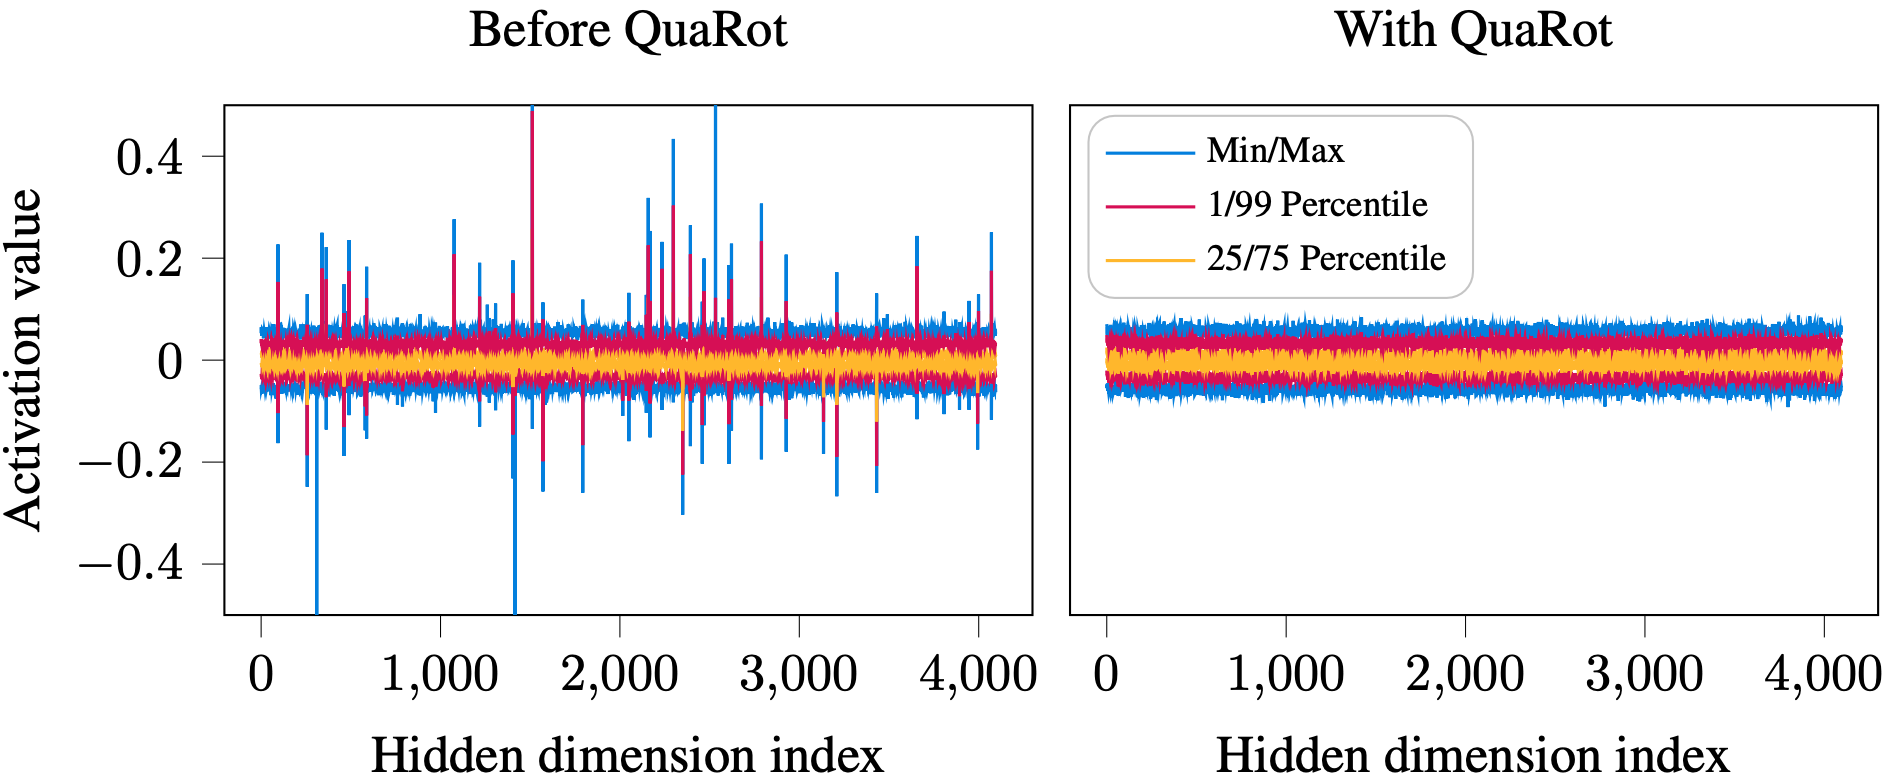
\includegraphics[width=.8\textwidth]{fig1.png}
    \caption{\label{fig:activation_dist} The distributions of activations at the input to the FFN block in \llamaSmall model, in the tenth layer. Left: using the default configuration as downloaded from Hugging Face. Right: after processing using QuaRot. The processed distribution has no outliers, leading to superior quantization. }
\end{figure}